\documentclass[11pt,fleqn]{article}

\usepackage[T1]{fontenc}
\usepackage{amsmath}
\usepackage{csquotes}
\usepackage{latexsym}
\usepackage{makeidx}
\usepackage{url}
\usepackage{xspace}
\usepackage{graphicx}
\usepackage{syntax}
\usepackage{textcomp}

\input{version}

% define home dir of the Curry system in order to locate tool manuals:
\newcommand{\curryhome}{../..}

%%% ------------------------------------------------------------------

\usepackage[colorlinks,linkcolor=blue]{hyperref}
\hypersetup{bookmarksopen=true}
\hypersetup{bookmarksopenlevel=0}
\hypersetup{pdftitle={PAKCS: The Portland Aachen Kiel Curry System}}
\hypersetup{pdfauthor={Michael Hanus}}
%\hypersetup{pdfstartview=Title}
\hypersetup{pdfstartview=FitH}
\usepackage{thumbpdf}

%%% ------------------------------------------------------------------

\setlength{\textwidth}{16.5cm}
\setlength{\textheight}{23cm}
\renewcommand{\baselinestretch}{1.1}
\setlength{\topmargin}{-1cm}
\setlength{\oddsidemargin}{0cm}
\setlength{\evensidemargin}{0cm}
\setlength{\marginparwidth}{0.0cm}
\setlength{\marginparsep}{0.0cm}

\newlength{\figurewidth}
\setlength{\figurewidth}{\textwidth}
\addtolength{\figurewidth}{-0.4cm}

% font for program texts
\renewcommand{\tt}{\usefont{OT1}{cmtt}{m}{n}\selectfont}
\newcommand{\codefont}{\small\tt}

\usepackage{listings}
\lstset{aboveskip=1.5ex,
        belowskip=1.5ex,
        showstringspaces=false, % no special string space
        mathescape=true,
        flexiblecolumns=false,
        xleftmargin=2ex,
        basewidth=0.52em,
        basicstyle=\small\ttfamily}

\lstset{literate={->}{{$\rightarrow{}\!\!\!$}}3
       }

\lstnewenvironment{curry}{}{}
\lstnewenvironment{currynomath}{\lstset{mathescape=false}}{} % Curry w/o math
\newcommand{\listline}{\vrule width0pt depth1.75ex}

% program text in normal text
\newcommand{\code}[1]{\mbox{\codefont #1}}

% program text in normal text with apostrophs
\newcommand{\ccode}[1]{``\code{#1}''}

\newcommand{\pindex}[1]{\index{#1@{\tt #1}}}  % program elements in index

\newcommand{\todo}[1]{\fbox{\sc To do: #1}}
\newcommand{\CYS}{PAKCS\xspace} % name of Curry system described here
\newcommand{\cyshome}{\mbox{\textit{pakcshome}}\xspace} % symbolic installation directory
\newcommand{\cb}{CurryBrowser\xspace}
\newcommand{\curryrc}{.pakcsrc} % name of the system's rc file

% allow underscores in programs:
\catcode`\_=\active
\let_=\sb
\catcode`\_=12

\newcommand{\translation}[1]{\bigskip\fbox{\begin{minipage}{15cm}\textbf{Translation: }{#1}\end{minipage}}\par\bigskip}

% produce an index:
\makeindex

\begin{document}
\sloppy

\begin{titlepage}
\pdfbookmark[1]{Title}{Title}
\begin{center}
\fbox{
\begin{minipage}[t]{\figurewidth}
\begin{center}\vspace{10ex}
{\Huge\bf PAKCS \pakcsversion}\\[4ex]
{\huge The Portland Aachen Kiel Curry System}\\[5ex]
{\huge User Manual}\\[2ex]
\pakcsversiondate\\[4ex]
\Large
Michael Hanus$^1$ [editor] \\[2ex]
{\large Additional Contributors:}\\[2ex]
Sergio Antoy$^2$ \\
Bernd Bra\ss{}el$^3$ \\
Martin Engelke$^4$ \\
Klaus H\"oppner$^5$ \\
Johannes Koj$^6$ \\
Philipp Niederau$^7$ \\
Bj\"orn Peem\"oller$^8$ \\
Ramin Sadre$^9$ \\
Frank Steiner$^{10}$ \\[4ex]
\normalsize
(1) University of Kiel, Germany, {\tt mh@informatik.uni-kiel.de} \\
(2) Portland State University, USA, {\tt antoy@cs.pdx.edu} \\
(3) University of Kiel, Germany, {\tt bbr@informatik.uni-kiel.de} \\
(4) University of Kiel, Germany, {\tt men@informatik.uni-kiel.de} \\
(5) University of Kiel, Germany, {\tt klh@informatik.uni-kiel.de} \\
(6) RWTH Aachen, Germany, {\tt johannes.koj@sdm.de} \\
(7) RWTH Aachen, Germany, {\tt philipp@navigium.de} \\
(8) University of Kiel, Germany, {\tt bjp@informatik.uni-kiel.de} \\
(9) RWTH Aachen, Germany, {\tt ramin@lvs.informatik.rwth-aachen.de} \\
(10) LMU Munich, Germany, {\tt fst@bio.informatik.uni-muenchen.de} \\[5ex]~
\end{center}
\end{minipage}}
\end{center}
\end{titlepage}

\pdfbookmark[1]{Contents}{Contents}
\tableofcontents

\clearpage
\addcontentsline{toc}{section}{Preface}
\section*{Preface}

This document describes \CYS (formerly called ``PACS''),
an implementation of the multi-paradigm language Curry,
jointly developed at the University of Kiel, the Technical University
of Aachen and Portland State University.
Curry is a universal programming language aiming at the amalgamation
of the most important declarative programming paradigms,
namely functional programming and logic programming.  
Curry combines in a seamless way features from functional programming
(nested expressions, lazy evaluation, higher-order functions),
logic programming (logical variables, partial data structures,
built-in search), and concurrent programming (concurrent evaluation
of constraints with synchronization on logical variables).
Moreover, the \CYS implementation of Curry also supports
constraint programming over various constraint domains,
the high-level implementation of distributed applications,
graphical user interfaces, and web services
(as described in more detail in \cite{Hanus99PPDP,Hanus00PADL,Hanus01PADL}).
Since \CYS compiles Curry programs into Prolog programs,
the availability of some of these features might depend on
the underlying Prolog system.

We assume familiarity with the ideas and features
of Curry as described in the Curry language definition \cite{Hanus15Curry}.
Therefore, this document only explains the use of the different
components of \CYS
and the differences and restrictions of \CYS
(see Section~\ref{sec-restrictions})
compared with the language Curry (Version 0.9.0).


\bigskip

\subsection*{Acknowledgements}

This work has been supported in part by the DAAD/NSF grant INT-9981317,
the NSF grants CCR-0110496 and CCR-0218224,
the Acci\'on Integrada hispano-alemana HA1997-0073,
and the DFG grants Ha 2457/1-2, Ha 2457/5-1, and Ha 2457/5-2.

Many thanks to the users of \CYS for bug reports, bug fixes, and improvements,
in particular, to Marco Comini, Sebastian Fischer, Massimo Forni,
Carsten Heine, Stefan Junge, Frank Huch, Parissa Sadeghi.


%%% Local Variables: 
%%% mode: latex
%%% TeX-master: "manual"
%%% End: 

\section{Overview of \CYS}

\subsection{General Use}
\label{sec-general}

This version of \CYS has been tested on Sun Solaris, Linux, and Mac OS X
systems. In principle, it should be also executable on other
platforms on which a Prolog system like SICStus-Prolog or SWI-Prolog exists
(see the file \code{INSTALL.html} in the \CYS directory
for a description of the necessary software to install \CYS).

All executable files required to use the different components
of \CYS are stored in the directory \code{\cyshome/bin}
(where \cyshome is the installation directory of the complete
\CYS installation). You should add this directory
to your path (e.g., by the \code{bash} command
\ccode{export PATH=\cyshome/bin:\$PATH}).

The source code of the Curry program
must be stored in a file with the suffix \ccode{.curry},
e.g., \code{prog.curry}. 
Literate programs must be stored in files with the extension \ccode{.lcurry}.
%They are automatically converted into corresponding
%\ccode{.curry} files by deleting all lines not starting 
%with \ccode{>} and removing the prefix \ccode{> } of the
%remaining lines.

Since the translation of Curry programs with \CYS creates
some auxiliary files (see Section~\ref{sec-auxfiles} for details),
you need write permission
in the directory where you have stored your Curry programs.
The auxiliary files for all Curry programs in the current
directory can be deleted by the command\pindex{cleancurry}
\begin{curry}
cleancurry
\end{curry}
(this is a shell script stored in the \code{bin} directory of the
\CYS installation, see above).
The command
\begin{curry}
cleancurry -r
\end{curry}
also deletes the auxiliary files in all subdirectories.



\subsection{Restrictions}
\label{sec-restrictions}

There are a few minor restrictions on Curry programs
when they are processed with \CYS:
\begin{itemize}
\item
\index{singleton variables}\index{variables!singleton}
\emph{Singleton pattern variables}, i.e., variables that occur only once
in a rule, should be denoted as an anonymous variable \ccode{_},
otherwise the parser will print a warning since this is a
typical source of programming errors.
\item
\CYS translates all \emph{local declarations} into global functions with
additional arguments (``lambda lifting'', see Appendix~D of the
Curry language report).
Thus, in the compiled target code, the definition of
functions with local declarations look different from
their original definition (in order to see the result
of this transformation, you can use the CurryBrowser, see
Section~\ref{sec-currybrowser}).
\item \index{tabulator stops}
Tabulator stops instead of blank spaces in source files are
interpreted as stops at columns 9, 17, 25, 33, and so on.
In general, tabulator stops should be avoided in source programs.
\item
Since PAKCS compiles Curry programs into Prolog programs,
non-deterministic computations are treated as in Prolog
by a backtracking strategy, which is known to be incomplete.
Thus, the order of rules could influence the ability
to find solutions for a given goal.
\item
Threads created by a concurrent conjunction are not executed
in a fair manner (usually, threads corresponding to leftmost constraints
are executed with higher priority).
\item
Encapsulated search\index{encapsulated search}: In order
to allow the integration of non-deterministic computations
in programs performing I/O at the top-level, \CYS supports
the search operators \code{findall}\pindex{findall}
and \code{findfirst}\pindex{findfirst}.
These and some other operators are available in the
library \code{Findall} (i.e., they are not part of the standard prelude).
In contrast to the general definition of encapsulated search
\cite{HanusSteiner98PLILP}, the current implementation suspends
the evaluation of \code{findall} and \code{findfirst}
until the argument does not contain unbound global variables.
Moreover, the evaluation of \code{findall} is strict,
i.e., it computes all solutions before returning the
complete list of solutions.

Since it is known that the result of these search operators might
depend on the evaluation strategy due to the combination of
sharing and lazy evaluation
(see \cite{BrasselHanusHuch04JFLP} for a detailed discussion),
it is recommended to use
\emph{set functions}\index{set functions} \cite{AntoyHanus09}
as a strategy-independent encapsulation of non-deterministic
computations.
Set functions compute the set of all results of a defined function
but do not encapsulate non-determinism occurring in the actual arguments.
See the library \code{SetFunctions}
(Section~\ref{Library:SetFunctions}) for more details.
\item
There is currently no general connection to external constraint solvers.
However, the \CYS compiler provides constraint
solvers for arithmetic and finite domain constraints
(see Appendix~\ref{sec:libraries}).
\end{itemize}

% Layout rule:
% (from Sergio's email of June 2, 1998)
%This is the general rule.  There are two kinds of syntactic
%constructs that rely on the offside rule.  One kind has a keyword
%indicating the end of the construct.  "let ... in" is the only
%representative of this kind.  Upon recognition of the keyword
%"in", all the constructs relying on the offide rule nested within
%the "let...in" are closed.  The other kind has no closing keyword.
%"where" and "choice" are the only constructs of this kind.
%Constructs of this kind can be closed only by indentation.  Any
%line, including a comment, indented less that the construct
%terminates it.  The indentation of "where", "choice" and "let" is
%the indentation of the first token following the keyword of the
%construct.
%



\subsection{Modules in \CYS}
\label{sec-modules}

\CYS searches for imported modules in various directories.
By default, imported modules are searched in the directory
of the main program and the system module directory
\ccode{\cyshome/lib}.
This search path can be extended
by setting the environment variable \code{CURRYPATH}\pindex{CURRYPATH}
(which can be also set in a \CYS session by the option
\ccode{:set path}\pindex{path}\pindex{:set path},
see below)
to a list of directory names separated by colons (\ccode{:}).
In addition, a local standard search path
can be defined in the \ccode{.pakcsrc} file
(see Section~\ref{sec-customization}).
Thus, modules to be loaded are searched in the following
directories (in this order, i.e., the first occurrence of a module file
in this search path is imported):
\begin{enumerate}
\item Current working directory (\ccode{.}) or directory prefix
of the main module (e.g., directory \ccode{/home/joe/curryprogs}
if one loads the Curry program \ccode{/home/joe/curryprogs/main}).
\item The directories enumerated in the environment variable \code{CURRYPATH}.
\item The directories enumerated in the \ccode{.pakcsrc} variable
      \ccode{libraries}.
\item The directory \ccode{\cyshome/lib}.
\end{enumerate}
The same strategy also applies to modules with a hierarchical
module name with the only difference that the hierarchy prefix
of a module name corresponds to a directory prefix of the module.
For instance, if the main module is stored in directory \code{MAINDIR}
and imports the module \code{Test.Func}, then the module stored in
\code{MAINDIR/Test/Func.curry} is imported (without setting
any additional import path) according to the
module search strategy described above.

Note that the standard prelude (\code{\cyshome/lib/Prelude.curry})
will be always implicitly imported to all modules if a module
does not contain an explicit import declaration for the module
\code{Prelude}.


%%% Local Variables: 
%%% mode: latex
%%% TeX-master: "manual"
%%% End: 

\section{\CYS: An Interactive Curry Development System}
\label{sec-curry2prolog}

\CYS\index{\CYS} is an interactive system to develop applications
written in Curry.
It is implemented in Prolog and compiles
Curry programs into Prolog programs. It contains various tools,
a source-level debugger,
solvers for arithmetic constraints over real numbers
and finite domain constraints, etc. The compilation process and the
execution of compiled programs is fairly efficient
if a good Prolog implementation like SICStus-Prolog is used.


\subsection{Invoking \CYS}
\label{sec:invoke-kics2}

To start \CYS, execute the command \ccode{pakcs}\pindex{pakcs}
(this is a shell script stored in
\code{\cyshome/bin} where \cyshome is the installation directory
of \CYS).
When the system is ready (i.e., when the prompt \ccode{Prelude>} occurs),
the prelude (\code{\cyshome/lib/Prelude.curry})
is already loaded, i.e., all definitions in the prelude are accessible.
Now you can type various commands (see next section)
or an expression to be evaluated.

One can also invoke \CYS with parameters.
These parameters are usual a sequence of commands
(see next section) that are executed before the user interaction
starts. For instance, the invocation
\begin{curry}
pakcs :load Mod :add List
\end{curry}
starts \CYS, loads the main module \code{Mod}, and adds the additional
module \code{List}.
The invocation
\begin{curry}
pakcs :load Mod :eval config
\end{curry}
starts \CYS, loads the main module \code{Mod}, and evaluates
the operation \code{config} before the user interaction starts.
As a final example, the invocation
\begin{curry}
pakcs :load Mod :save :quit
\end{curry}
starts \CYS, loads the main module \code{Mod}, creates an executable,
and terminates \CYS. This invocation could be useful in ``make'' files
for systems implemented in Curry.

It is also possible to overwrite the values defined in the
configuration file \ccode{.pakcsrc}
(see Section~\ref{sec-customization})
when starting \CYS. For this purpose, one can put options of the form
\begin{curry}
pakcs -Dname=val
\end{curry}
where \code{name} is a property defined in the configuration file
and \code{val} its new value.


\subsection{Commands of \CYS}
\label{sec:pakcs-commands}

The {\bf most important commands} of \CYS are
(it is sufficient to type a unique prefix of a command if it is unique,
e.g., one can type \ccode{:r} instead of \ccode{:reload}):

\begin{description}
\item[\fbox{\code{:help}}]\pindex{:help}
Show a list of all available commands.

\item[\fbox{\code{:load $prog$}}]\pindex{:load}
Compile and load the program stored in \code{$prog$.curry}
together with all its imported modules.
If this file does not exist, the system looks for a FlatCurry
file \code{$prog$.fcy} and compiles from this intermediate representation.
If the file \code{$prog$.fcy} does not exists, too, the system looks
for a file \code{$prog$_flat.xml} containing a FlatCurry program in
XML representation (compare command \ccode{:xml}\pindex{:xml}),
translates this into a FlatCurry file \code{$prog$.fcy}
and compiles from this intermediate representation.

\item[\fbox{\code{:reload}}]\pindex{:reload}
Recompile all currently loaded modules.

\item[\fbox{\code{:add} $m_1 \ldots m_n$}]\pindex{:add}
Add modules $m_1,\ldots,m_n$ to the set of currently loaded modules
so that their exported entities are available in the top-level environment.

\item[\fbox{$expr$}] Evaluate the expression $expr$ to normal form
and show the computed results. Since \CYS
compiles Curry programs into Prolog programs,
non-deterministic computations are implemented by backtracking.
Therefore, computed results are shown one after the other.
In the \emph{interactive mode} (which can be set in the
configuration file \ccode{\curryrc} or by setting the option
\code{interactive}, see below), you will be asked
after each computed result whether
you want to see the next alternative result or all alternative results.
The default answer value for this question can be defined
in the configuration file \ccode{\curryrc} file
(see Section~\ref{sec-customization}).

\textbf{Free variables in initial expressions} must be declared as
in Curry programs
(if the free variable mode\index{free variable mode} is not turned on,
see option \ccode{+free} below).
Thus, in order to see the results of their bindings,
they must be introduced by a \ccode{where\ldots{}free} declaration.
For instance, one can write
\begin{curry}
not b where b free
\end{curry}
in order to obtain the following bindings and results:
\begin{curry}
{b = True} False
{b = False} True
\end{curry}
Without these declarations, an error is reported in order to
avoid the unintended introduction of free variables in initial expressions
by typos.

\item[\fbox{:eval $expr$}]\pindex{:eval}
Same as $expr$. This command might be useful when putting
commands as arguments when invoking \code{pakcs}.

\item[\fbox{:define $x$=$expr$}]
Define the identifier $x$ as an abbreviation for the expression $expr$
which can be used in subsequent expressions. The identifier $x$
is visible until the next \code{load} or \code{reload} command.

\item[\fbox{\code{:quit}}]\pindex{:quit} Exit the system.
\end{description}
%
\bigskip
%
There are also a number of {\bf further commands} that are often
useful:
%
\begin{description}
\item[\fbox{\code{:type $expr$}}]\pindex{:type}
Show the type of the expression $expr$.

\item[\fbox{\code{:browse}}]\pindex{:browse}
Start the CurryBrowser to analyze the currently loaded
module together with all its imported modules
(see Section~\ref{sec-currybrowser} for more details).

\item[\fbox{\code{:edit}}]\pindex{:edit}
Load the source code of the current main module into a text editor.
If the variable \code{editcommand} is set in the
configuration file \ccode{.pakcsrc}
(see Section~\ref{sec-customization}),
its value is used as an editor command, otherwise
the environment variable \ccode{EDITOR}
or a default editor (e.g., \ccode{vi}) is used.

\item[\fbox{\code{:edit $file$}}]\pindex{:edit}
Load file $file$ into a text editor which is defined
as in the command \ccode{:edit}.

\item[\fbox{\code{:interface}}]\pindex{:interface}
Show the interface of the currently loaded
module, i.e., show the names of all imported modules,
the fixity declarations of all exported operators,
the exported datatypes declarations and the types
of all exported functions.

\item[\fbox{\code{:interface $prog$}}]\pindex{:interface}
Similar to \ccode{:interface}
but shows the interface of the module \ccode{$prog$.curry}.
If this module does not exist, this command looks in the
system library directory of \CYS for a module with this name,
e.g., the command \ccode{:interface FlatCurry} shows the interface
of the system module \code{FlatCurry} for meta-programming
(see Appendix~\ref{sec-flatcurry}).

\item[\fbox{\code{:usedimports}}]\pindex{:usedimports}
Show all calls to imported functions in the currently loaded module.
This might be useful to see which import declarations are really necessary.

\item[\fbox{\code{:modules}}]\pindex{:modules}
Show the list of all currently loaded modules.

\item[\fbox{\code{:programs}}]\pindex{:programs}
Show the list of all Curry programs that are available in the load path.

\item[\fbox{\code{:set $option$}}]\pindex{:set}
Set or turn on/off a specific option
of the \CYS environment (see \ref{sec:options} for a description
of all options). Options are turned on by the prefix
\ccode{+} and off by the prefix \ccode{-}. Options that can only
be set (e.g., \code{printdepth}) must not contain a prefix.

\item[\fbox{\code{:set}}]\pindex{:set}
Show a help text on the possible options
together with the current values of all options.

\item[\fbox{\code{:show}}]\pindex{:show}
Show the source text of the currently loaded Curry program.
If the variable \code{showcommand} is set in the
configuration file \ccode{.pakcsrc}
(see Section~\ref{sec-customization}),
its value is used as a command to show the source text,
otherwise the environment variable \code{PAGER} or the standard command
\ccode{cat} is used.
If the source text is not available
(since the program has been directly compiled from a FlatCurry
or XML file), the loaded program is decompiled and
the decompiled Curry program text is shown.

\item[\fbox{\code{:show $m$}}]\pindex{:show}
Show the source text of module $m$ which must be accessible
via the current load path.

\item[\fbox{\code{:source $f$}}]\pindex{:source}
Show the source code of function $f$ (which must be visible
in the currently loaded module) in a separate window.

\item[\fbox{\code{:source $m$.$f$}}]\pindex{:source}
Show the source code of function $f$ defined in module $m$
in a separate window.

\item[\fbox{\code{:cd $dir$}}]\pindex{:cd}
Change the current working directory to $dir$.

\item[\fbox{\code{:dir}}]\pindex{:dir} Show the names of all Curry programs
in the current working directory.

\item[\fbox{\code{:!$cmd$}}]\pindex{:"!} Shell escape: execute $cmd$ in a Unix shell.

\item[\fbox{\code{:save}}]\pindex{:save} Save the currently loaded
program as an executable evaluating the main expression \ccode{main}.
The executable is stored in the file \code{Mod}
if \code{Mod} is the name of the currently loaded main module.

\item[\fbox{\code{:save $expr$}}]\pindex{:save} Similar as \ccode{:save}
but the expression $expr$ (typically: a call to the main
function) will be evaluated by the executable.

\item[\fbox{\code{:fork $expr$}}]\pindex{:fork}
The expression $expr$, which must be of type \ccode{IO ()},
is evaluated in an independent process which runs in
parallel to the current \CYS process.
All output and error messages from this new process are suppressed.
This command is useful to test distributed Curry programs
(see Appendix~\ref{sec-ports}) where one can start
a new server process by this command. The new process
will be terminated when the evaluation of the expression $expr$
is finished.

\item[\fbox{\code{:coosy}}]\pindex{:coosy}
Start the Curry Object Observation System COOSy,
a tool to observe the execution of Curry programs.
This commands starts a graphical user interface to show
the observation results and adds to the load path the directory
containing the modules that must be imported in order to annotate
a program with observation points.
Details about the use of COOSy can be found in the
COOSy interface (under the ``Info'' button), and details
about the general idea of observation debugging and the implementation
of COOSy can be found in \cite{BrasselChitilHanusHuch04PADL}.

\item[\fbox{\code{:xml}}]\pindex{:xml}
Translate the currently loaded program module into an XML representation
according to the format described in
\url{http://www.informatik.uni-kiel.de/~curry/flat/}.
Actually, this yields an implementation-independent
representation of the corresponding FlatCurry program
(see Appendix~\ref{sec-flatcurry} for a description of FlatCurry).
If $prog$ is the name of the currently loaded program,
the XML representation will be written into the file \ccode{$prog$_flat.xml}.

\item[\fbox{\code{:peval}}]\pindex{:peval}
Translate the currently loaded program module into an equivalent
program where some subexpressions are partially evaluated
so that these subexpressions are (hopefully) more efficiently executed.
An expression $e$ to be partially evaluated
must be marked in the source program by \code{(PEVAL e)}
(where \code{PEVAL} is defined as the identity function in the prelude
so that it has no semantical meaning).

The partial evaluator
translates a source program \code{$prog$.curry} into the
partially evaluated program in intermediate representation
stored in \code{$prog$_pe.fcy}. The latter program is implicitly loaded
by the \code{peval} command so that the partially evaluated program
is directly available. The corresponding source program
can be shown by the \code{show} command (see above).

The current partial evaluator is an experimental prototype
(so it might not work on all programs) based on the ideas
described in \cite{AlbertAlpuenteHanusVidal99LPAR,AlbertHanusVidal00LPAR,%
AlbertHanusVidal01FLOPS,AlbertHanusVidal02JFLP}.

\end{description}


\subsection{Options of \CYS}
\label{sec:options}

The following options (which can be set by the command \ccode{:set})
are currently supported:

\begin{description}
\item[\fbox{\code{+/-debug}}]\pindex{debug} Debug mode.
\index{debug mode}
In the debug mode, one can trace the evaluation of an expression,
setting spy points (break points) etc.\ (see the commands
for the debug mode described below).

\item[\fbox{\code{+/-free}}]\pindex{free}
Free variable mode.\index{free variable mode}
If the free variable mode is off (default), then
free variables occurring in initial expressions entered in the
\CYS environment must always be declared by \ccode{where\ldots{}free}.
This avoids the introduction of free variables in initial expressions
by typos (which might lead to the exploration of infinite search spaces).
If the free variable mode is on, each undefined symbol occurring
in an initial expression is considered as a free variable.
In this case, the syntax of accepted initial expressions
is more restricted.
In particular, lambda abstractions, \code{let}s and list comprehensions
are not allowed if the free variable mode is on.

\item[\fbox{\code{+/-printfail}}]\pindex{printfail} Print failures.
If this option is set, failures occurring during evaluation
(i.e., non-reducible demanded subexpressions) are printed.
This is useful to see failed reductions due to partially
defined functions or failed unifications.
Inside encapsulated search (e.g., inside evaluations of
\code{findall} and \code{findfirst}), failures are not printed
(since they are a typical programming technique there).
Note that this option causes some overhead in execution time
and memory so that it could not be used in larger applications.

\item[\fbox{\code{+/-allfails}}]\pindex{allfails}
If this option is set, \emph{all} failures
(i.e., also failures on backtracking and failures
of enclosing functions that fail due to the failure of an argument
evaluation) are printed if the option \code{printfail} is set.
Otherwise, only the first failure (i.e., the first non-reducible
subexpression) is printed.

\item[\fbox{\code{+/-consfail}}]\pindex{consfail} Print constructor failures.
If this option is set, failures due to application of
functions with non-exhaustive pattern matching or failures
during unification (application of \ccode{=:=}) are shown.
Inside encapsulated search (e.g., inside evaluations of
\code{findall} and \code{findfirst}), failures are not printed
(since they are a typical programming technique there).
In contrast to the option \code{printfail},
this option creates only a small overhead in execution time
and memory use.

\item[\fbox{\code{+consfail all}}]\pindex{consfail}
Similarly to \ccode{+consfail}, but the complete trace
of all active (and just failed) function calls from the main function
to the failed function are shown.

\item[\fbox{\code{+consfail file:$f$}}]\pindex{consfail}
Similarly to \ccode{+consfail all}, but the complete fail trace
is stored in the file $f$. This option is useful in non-interactive
program executions like web scripts.

\item[\fbox{\code{+consfail int}}]\pindex{consfail}
Similarly to \ccode{+consfail all}, but after each failure occurrence,
an interactive mode for exploring the fail trace is started
(see help information in this interactive mode).
When the interactive mode is finished, the program execution
proceeds with a failure.

\item[\fbox{\code{+/-compact}}]\pindex{compact}
Reduce the size of target programs by using the
parser option \ccode{--compact}
(see Section~\ref{sec-pakcspp} for details about this option).

\item[\fbox{\code{+/-interactive}}]\pindex{interactive}
Turn on/off the interactive mode.
In the interactive mode, the next non-deterministic value
is computed only when the user requests it.
Thus, one has also the possibility to terminate the
enumeration of all values after having seen some values.
The default value for this option can be set in the
configuration file \ccode{\curryrc} (initially, the interactive
mode is turned off).

\item[\fbox{\code{+/-first}}]\pindex{first}
Turn on/off the first-only mode.
In the first-only mode, only the first value
of the main expression is printed (instead of all values).

\item[\fbox{\code{+/-profile}}]\pindex{profile} Profile mode.
If the profile mode is on, then information about
the number of calls, failures, exits etc.\ are collected for
each function during the debug mode (see above) and shown
after the complete execution (additionaly, the result is stored
in the file \code{$prog$.profile} where $prog$ is the current main program).
The profile mode has no effect outside the debug mode.


\item[\fbox{\code{+/-suspend}}] Suspend mode (initially, it is off).
If the suspend mode is on, all suspended expressions
(if there are any) are shown (in their internal representation) at the end
of a computation.

\item[\fbox{\code{+/-time}}]\pindex{time} Time mode. If the time mode is on,
the cpu time and the elapsed time
of the computation is always printed together with the result
of an evaluation.

\item[\fbox{\code{+/-verbose}}] Verbose mode (initially, it is off).
If the verbose mode is on,
the initial expression of a computation (together with its type)
is printed before this expression is evaluated.

\item[\fbox{\code{+/-warn}}]\pindex{warn} Parser warnings. If the parser
warnings are turned on (default), the parser will print
warnings about variables that occur only once in a program rule
(see Section~\ref{sec-restrictions})
or locally declared names that shadow the definition of
globally declared names. If the parser warnings are switched off,
these warnings are not printed during the reading of a Curry program.

\item[\fbox{\code{path $path$}}]\pindex{path} Set the additional search path
for loading modules to $path$.
Note that this search path is only used for loading modules
inside this invocation of \CYS, i.e., the environment variable
\ccode{CURRYPATH}\pindex{CURRYPATH} (see also Section~\ref{sec-modules})
is set to $path$ in this invocation of \CYS.

The path is a list of directories separated by \ccode{:}.
The prefix \ccode{\char126} is replaced by the home directory as
in the following example:
\begin{curry}
:set path aux:~/tests
\end{curry}
Relative directory names are replaced by absolute ones
so that the path is independent of later changes of the
current working directory.

\item[\fbox{\code{printdepth $n$}}]\pindex{printdepth}
Set the depth for printing terms to the value \code{n} (initially: 10).
In this case subterms with a depth greater than \code{n} are abbreviated
by dots when they are printed as a result of a computation
or during debugging. A value of \code{0} means infinite depth
so that the complete terms are printed.

\item[\fbox{\code{v$n$}}]\pindex{v}\index{verbosity}
Set the verbosity level to $n$. The following values are allowed
for $n$:
\begin{description}
\item[$n=0$:] Do not show any messages (except for errors).
\item[$n=1$:] Show only messages of the front-end, like loading
of modules.
\item[$n=2$:]
Show also messages of the back end, like loading intermediate files
or generating Prolog target files.
\item[$n=3$:]
Show also messages related to loading Prolog files and libraries
into the run-time systems and other intermediate messages and results.
\end{description}

\item[\fbox{\code{safe}}]\pindex{safe}
Turn on the safe execution mode.
In the safe execution mode, the initial goal is
not allowed to be of type \code{IO} and the program should not
import the module \code{Unsafe}.
Furthermore, the allowed commands are
\code{eval}, \code{load}, \code{quit}, and \code{reload}.
This mode is useful to use \CYS in uncontrolled environments,
like a computation service in a web page, where \CYS could
be invoked by
\begin{curry}
pakcs :set safe
\end{curry}

\item[\fbox{\code{parser $opts$}}]\pindex{parser}
Define additional options passed to the \CYS front end, i.e.,
the parser program \code{\cyshome/bin/cymake}.
For instance, setting the option
\begin{curry}
:set parser -F --pgmF=transcurry
\end{curry}
has the effect that each Curry module to be compiled is
transformed by the preprocessor command \code{transcurry}
into a new Curry program which is actually compiled.

\item[\fbox{\code{args $arguments$}}]\pindex{args}
Define run-time arguments for the evaluation
of the main expression.
For instance, setting the option
\begin{curry}
:set args first second
\end{curry}
has the effect that the I/O operation \code{getArgs}
(see library \code{System} (Section~\ref{Library:System})
returns the value \code{["first","second"]}.

\end{description}
%
\bigskip
%
\CYS can also execute programs in the {\bf debug mode}.
\index{debug mode}\pindex{debug}
The debug mode is switched on by setting the \code{debug} option
with the command \ccode{:set +debug}. In order to switch
back to normal evaluation of the program, one has to execute
the command \ccode{:set -debug}.

In the debug mode, \CYS offers the following additional options:
%
\begin{description}
\item[\fbox{\code{+/-single}}]\pindex{single}
Turn on/off single mode for debugging.
If the single mode is on, the evaluation of an expression
is stopped after each step and the user is asked how to proceed
(see the options there).

\item[\fbox{\code{+/-trace}}]\pindex{trace}
Turn on/off trace mode for debugging.
If the trace mode is on, all intermediate expressions occurring
during the evaluation of an expressions are shown.

\item[\fbox{\code{spy $f$}}]\pindex{spy}
Set a spy point (break point) on the
function $f$. In the single mode, you can ``leap'' from spy point
to spy point (see the options shown in the single mode).

\item[\fbox{\code{+/-spy}}]\pindex{spy} Turn on/off spy mode for debugging.
If the spy mode is on, the single mode is automatically activated
when a spy point is reached.
\end{description}


\subsection{Using \CYS in Batch Mode}

Although \CYS is primarily designed as an interactive system,
it can also be used to process data in batch mode.
For example, consider a Curry program, say \code{myprocessor}, that
reads argument strings from the command line and processes them.
Suppose the entry point is a function called \code{just_doit}
that takes no arguments. Such a processor can be invoked from
the shell as follows:
\begin{curry}
> pakcs :set args string1 string2 :load myprocessor.curry :eval just_doit :quit
\end{curry}
The \ccode{:quit} directive in necessary to avoid \CYS going
into interactive mode after the
excution of the expression being evaluated.
The actual run-time arguments (\code{string1}, \code{string2})
are defined by setting the option \code{args} (see above).

Here is an example to use \CYS in this way:
\begin{curry}
> pakcs :set args Hello World :add System :eval "getArgs >>= putStrLn . unwords" :quit
Hello World
>
\end{curry}


\subsection{Command Line Editing}

In order to have support for line editing or history functionality
in the command line of \CYS (as often supported by the \code{readline}
library), you should have the Unix command \code{rlwrap} installed
on your local machine.
If \code{rlwrap} is installed, it is used by \CYS if called on a terminal.
If it should not be used (e.g., because it is executed
in an editor with \code{readline} functionality), one can
call \CYS with the parameter \ccode{--noreadline}.


\subsection{Customization}
\label{sec-customization}

In order to customize the behavior of \CYS to your own preferences,
there is a configuration file which is read by \CYS when it is invoked.
When you start \CYS for the first time, a standard version of
this configuration file is copied with the name
\ccode{.pakcsrc}\pindex{pakcsrc}\pindex{.pakcsrc}
into your home directory. The file contains definitions
of various settings, e.g., about showing warnings, progress messages etc.
After you have started \CYS for the first time, look into this file
and adapt it to your own preferences.


\subsection{Emacs Interface}

Emacs is a powerful programmable editor suitable for program development.
It is freely available for many platforms
(see \url{http://www.emacs.org}).
The distribution of \CYS contains also a special
\emph{Curry mode}\index{Curry mode}\index{Emacs}
that supports the development of Curry programs in
the Emacs environment.
This mode includes support for syntax highlighting,
finding declarations in the current buffer, and
loading Curry programs into \CYS
in an Emacs shell.

The Curry mode has been adapted from a similar mode for Haskell programs.
Its installation is described in the file \code{README}
in directory \ccode{\cyshome/tools/emacs} which also contains
the sources of the Curry mode and a short description about
the use of this mode.


%%% Local Variables: 
%%% mode: latex
%%% TeX-master: "manual"
%%% End: 

\section{Extensions}
\label{sec-extensions}

\CYS supports some extensions in Curry programs that are not (yet)
part of the definition of Curry. These extensions are described below.

\subsection{Recursive Variable Bindings}

Local variable declarations (introduced by \code{let}\pindex{let}
or \code{where}\pindex{where}) can be (mutually) recursive in \CYS.
For instance, the declaration
\begin{curry}
ones5 = let ones = 1 : ones
         in take 5 ones
\end{curry}
introduces the local variable \code{ones} which is bound
to a \emph{cyclic structure}\index{cyclic structure}
representing an infinite list of \code{1}'s.
Similarly, the definition
\begin{curry}
onetwo n = take n one2
 where
   one2 = 1 : two1
   two1 = 2 : one2
\end{curry}
introduces a local variables \code{one2} that represents
an infinite list of alternating \code{1}'s and \code{2}'s
so that the expression \code{(onetwo 6)} evaluates to \code{[1,2,1,2,1,2]}.


\subsection{Functional Patterns}

Functional patterns \cite{AntoyHanus05LOPSTR} are a useful extension
to code operations in a more readable way. Furthermore,
defining operations with functional patterns avoids problems
caused by strict equality (\ccode{=:=}) and leads to programs
that are potentially more efficient.

Consider the definition of an operation to compute the last element
of a list \code{xs} based on the prelude operation \ccode{++}
for list concatenation:
\begin{curry}
last xs | _++[y] =:= xs  = y   where y free
\end{curry}
Since the equality constraint \ccode{=:=} evaluates both sides
to a constructor term, all elements of the list \code{xs} are
fully evaluated in order to satisfy the constraint.

Functional patterns can help to improve this computational behavior.
A \emph{functional pattern}\index{functional pattern}\index{pattern!functional}
is a function call at a pattern position. With functional patterns,
we can define the operation \code{last} as follows:
\begin{curry}
last (_++[y]) = y
\end{curry}
This definition is not only more compact but also avoids the complete
evaluation of the list elements: since a functional pattern is considered
as an abbreviation for the set of constructor terms obtained by all
evaluations of the functional pattern to normal form (see
\cite{AntoyHanus05LOPSTR} for an exact definition), the previous
definition is conceptually equivalent to the set of rules
\begin{curry}
last [y] = y
last [_,y] = y
last [_,_,y] = y
$\ldots$
\end{curry}
which shows that the evaluation of the list elements is not demanded
by the functional pattern.

In general, a pattern of the form \code{($f$ $t_1$\ldots$t_n$)} ($n>0$)
is interpreted as a functional pattern if $f$ is not a visible constructor
but a defined function that is visible in the scope of the pattern.

It is also possible to combine functional patterns with
as-patterns.\index{as-pattern}\pindex{"@}
Similarly to the meaning of as-patterns
in standard constructor patterns,
as-patterns in functional patterns are interpreted
as a sequence of pattern matching where the variable of the as-pattern
is matched before the given pattern is matched.
This process can be described by introducing an auxiliary operation
for this two-level pattern matching process.
For instance, the definition
\begin{curry}
f (_ ++ x@[(42,_)] ++ _) = x
\end{curry}
is considered as syntactic sugar for the expanded definition
\begin{curry}
f (_ ++ x ++ _) = f' x
 where
  f' [(42,_)] = x
\end{curry}
However, as-patterns are usually implemented
in a more efficient way without introducing auxiliary operations.


\paragraph{Optimization of programs containing functional patterns.}
Since functions patterns can evaluate to non-linear constructor terms,
they are dynamically checked for multiple occurrences of
variables which are, if present, replaced by equality constraints
so that the constructor term is always linear
(see \cite{AntoyHanus05LOPSTR} for details).
Since these dynamic checks are costly and not necessary for
functional patterns that are guaranteed to evaluate to linear terms,
there is an optimizer for functional patterns that checks
for occurrences of functional patterns that evaluate always to
linear constructor terms and replace such occurrences
with a more efficient implementation.
This optimizer can be enabled by the following possibilities:
\begin{itemize}
\item
Set the environment variable \code{FCYPP} to \ccode{--fpopt}
before starting \CYS, e.g., by the shell command
\begin{curry}
export FCYPP="--fpopt"
\end{curry}
Then the functional pattern optimization is applied if programs are compiled
and loaded in \CYS.
\item
Put an option into the source code:
If the source code of a program
contains a line with a comment of the form (the comment
must start at the beginning of the line)
\begin{curry}
{-# PAKCS_OPTION_FCYPP --fpopt #-}
\end{curry}
then the functional pattern optimization is applied
if this program is compiled and loaded in \CYS.
\end{itemize}
The optimizer also report errors in case of wrong uses of functional patterns
(i.e., in case of a function $f$ defined with functional patterns that
recursively depend on $f$).


\subsection{Order of Pattern Matching}

Curry allows multiple occurrences of pattern variables
in standard patterns. These are an abbreviation of equational constraints
between pattern variables.
Functional patterns might also contain multiple occurrences of
pattern variables.
For instance, the operation
\begin{curry}
f (_++[x]++_++[x]++_) = x
\end{curry}
returns all elements with at least two occurrences in a list.

If functional patterns as well as multiple occurrences of
pattern variables occur in a pattern defining an operation,
there are various orders to match an expression against such
an operation. In the current implementation, the order
is as follows:
\begin{enumerate}
\item Standard pattern matching: First, it is checked whether
the constructor patterns match. Thus, functional patterns
and multiple occurrences of pattern variables are ignored.
\item Functional pattern matching: In the next phase,
functional patterns are matched but occurrences of standard
pattern variables in the functional patterns are ignored.
\item Non-linear patterns: If standard and functional pattern matching
is successful, the equational constraints which correspond
to multiple occurrences pattern variables are solved.
\item Guards: Finally, the guards supplied by the programmer
are checked.
\end{enumerate}
The order of pattern matching should not influence the computed
result. However, it might have some influence on the termination
behavior of programs, i.e., a program might not terminate
instead of finitely failing.
In such cases, it could be necessary to consider the influence
of the order of pattern matching. Note that other orders of pattern matching
can be obtained using auxiliary operations.



\subsection {Records}
\label{records}

A record is a data structure for bundling several data of various types.
It consists of typed data fields where each field is associated with
a unique label. These labels can be used to construct, select or update
fields in a record.


Unlike labeled data fields in Haskell, records are
not syntactic sugar but a real extension of the
language\footnote{The current version allows to transform records
  into abstract data types. Future extensions may not have
  this facility.}.
The basic concept is described in \cite{Leijen05} but the current
version does not yet provide all features mentioned there.
The restrictions are explained in Section~\ref{sec-restrinrecs}.

\subsubsection{Record Type Declaration}
\label{sec-recordtypedecl}

It is necessary to declare a record type before a record
can be constructed or used. The declaration has the following form:
\begin{curry}
type $R$ $\alpha_1$ $\ldots$ $\alpha_n$ = { $l_1$ :: $\tau_1$,$\ldots$, $l_m$ :: $\tau_m$ }
\end{curry}
It introduces a new $n$-ary record type $R$ which represents a
record consisting of $m$ fields. Each field has a unique label $l_i$
representing a value of the type $\tau_i$. Labels
are identifiers which refer to the corresponding
fields. The following examples define some record types:
\begin{curry}
type Person = {name :: String, age :: Int}
type Address = {person :: Person, street :: String, city :: String}
type Branch a b = {left :: a, right :: b}
\end{curry}
It is possible to summarize different labels which have the same
type. For instance, the record \code{Address} can also be declared as follows:
\begin{curry}
type Address = {person :: Person, street,city :: String}
\end{curry}
The fields can occur in an arbitrary order. The example above
can also be written as
\begin{curry}
type Address = {street,city :: String, person :: Person}
\end{curry}
The record type can be used in every type expression to represent
the corresponding record, e.g.
\begin{curry}
data BiTree = Node (Branch BiTree BiTree) | Leaf Int
\end{curry}
\begin{curry}
getName :: Person -> String
getName $\ldots$
\end{curry}

Labels can only be used in the context of
records. They do not share the name space with
functions/constructors/variables or type constructors/type variables.
For instance it is possible to use
the same identifier for a label and a function at the same time. Label
identifiers cannot be shadowed by other identifiers.

Like in type synonym declarations, recursive or mutually
dependent record declarations are not allowed. Records can only
be declared at the top level. Further restrictions are described in
section \ref{sec-restrinrecs}.


\subsubsection{Record Construction}
\label{sec-recordconstr}

The record construction generates a record with initial values for
each data field. It has the following form:
\begin{curry}
{ $l_1$ := $v_1$,$\ldots$, $l_m$ := $v_m$ }
\end{curry}
It generates a record where each label $l_i$ refers to the
value $v_i$. The type of the record results from the record type
declaration where the labels $l_i$ are defined.
A mix of labels from different
record types is not allowed. All labels must be specified with
exactly one assignment. Examples for record constructions are
\begin{curry}
{name := "Johnson", age := 30}     -- generates a record of type 'Person'
{left := True, right := 20}        -- generates a record of type 'Branch'
\end{curry}
Assignments to labels can occur in an arbitrary order. For instance a
record of type \code{Person} can also be generated as follows:
\begin{curry}
{age := 30, name := "Johnson"}     -- generates a record of type 'Person'
\end{curry}
Unlike labeled fields in record type declarations,
record constructions can be used in expressions without any restrictions
(as well as all kinds of record expressions). For instance the following
expression is valid:
\begin{curry}
{person := {name := "Smith", age := 20},   -- generates a record of
 street := "Main Street",                  -- type 'Address'
 city   := "Springfield"}
\end{curry}


\subsubsection{Field Selection}
\label{sec-fieldsel}

The field selection is used to extract data from records.
It has the following form:
\begin{curry}
$r$ :> $l$
\end{curry}
It returns the value to which the label $l$ refers to from the
record expression $r$. The label must occur in the declaration of
the record type of $r$.
An example for a field selection is:
\begin{curry}
pers :> name
\end{curry}
This returns the value of the label \code{name} from the record \code{pers}
(which has the type \code{Person}).
Sequential application of field selections are also possible:
\begin{curry}
addr :> person :> age
\end{curry}
The value of the label \code{age} is extracted from a record which itself
is the value of the label \code{person} in the record \code{addr}
(which has the type \code{Address}).


\subsubsection{Field Update}
\label{sec-fieldupd}

Records can be updated by reassigning a new value to a label:
\begin{curry}
{$l_1$ := $v_1$,$\ldots$, $l_k$ := $v_k$ | $r$}
\end{curry}
The label $l_i$ is associated with the new value $v_i$ which
replaces the current value in the record $r$.
The labels must occur in the declaration
of the record type of $r$. In contrast to record constructions,
it is not necessary to specify all labels of a record.
Assignments can occur in an arbitrary order. It is not allowed to
specify more than one assignment for a label in a record update.
Examples for record updates are:
\begin{curry}
{name := "Scott", age := 25 | pers}
{person := {name := "Scott", age := 25 | pers} | addr}
\end{curry}
In these examples \code{pers} is a record of type \code{Person} and \code{addr}
is a record of type \code{Address}.


\subsubsection{Records in Pattern Matching}
\label{sec-recsinpm}

It is possible to apply pattern matching to records (e.g., in functions,
let expressions or case branches). Two kinds of record patterns
are available:
\begin{curry}
{$l_1$ = $p_1$,$\ldots$, $l_n$ = $p_n$}
{$l_1$ = $p_1$,$\ldots$, $l_k$ = $p_k$ | _}
\end{curry}
In both cases each label $l_i$ is specified with a pattern $p_i$.
All labels must occur only once in the record pattern.
The first case is used to match the whole record. Thus, all labels
of the record must occur in the pattern.
The second case is used to match only a part of
the record. Here it is not necessary to specify all labels.
This case is represented by a vertical bar followed by the underscore
(anonymous variable). It is
not allowed to use a pattern term instead of the underscore.


When trying to match a record against a record pattern, the
patterns of the specified labels are matched against
the corresponding values in the record expression. On success, all pattern
variables occurring in the patterns are replaced by their actual expression.
If none of the patterns matches, the computation fails.


Here are some examples of pattern matching with records:
\begin{curry}
isSmith30 :: Person -> Bool
isSmith30 {name = "Smith", age = 30} = True
\end{curry}
\begin{curry}
startsWith :: Char -> Person -> Bool
startsWith c {name = (d:_) | _} = c == d
\end{curry}
\begin{curry}
getPerson :: Address -> Person
getPerson {person = p | _} = p
\end{curry}
As shown in the last example, a field selection can also be obtained
by pattern matching.


\subsubsection{Export of Records}
\label{sec-exprecs}

Exporting record types and labels is very similar to exporting
data types and constructors. There are three ways
to specify an export:
\begin{itemize}
\item \code{module $M$ (\ldots, $R$, \ldots) where} \\
  exports the record $R$ without any of its labels.
\item \code{module $M$ (\ldots, $R$(..), \ldots) where} \\
  exports the record $R$ together with all its labels.
\item \code{module $M$ (\ldots, $R$($l_1$,\ldots,$l_k$), \ldots) where} \\
  exports the record $R$ together with the labels $l_1$, \ldots, $l_k$.
\end{itemize}
%
Note that imported labels cannot be overwritten in record declarations
of the importing module. It is also not possible to import equal labels
from different modules.


\subsubsection{Restrictions in the Usage of Records}
\label{sec-restrinrecs}

In contrast to the basic concept in \cite{Leijen05}, \CYS/Curry provides a
simpler version of records. Some of the features described there are
currently not supported or even restricted.

\begin{itemize}
\item Labels must be unique within the whole scope of the program.
  In particular, it is not allowed to define the same label within
  different records, not even when they are imported from other
  modules. However, it is possible to use equal identifiers for other
  entities without restrictions, since labels have an independent
  name space.
\item The record type representation with labeled fields can only be
  used as the right-hand-side of a record type declaration. It is
  not allowed to use it in any other type annotation.
\item Records are not extensible or reducible. The structure of a
  record is specified in its record declaration and cannot be
  modified at the runtime of the program.
\item Empty records are not allowed.
\item It is not allowed  to use a pattern term
  at the right side of the vertical bar in a record pattern
  except for the underscore (anonymous pattern variable).
\item Labels cannot be sequentially associated with multiple values
  (record fields do not behave like stacks).
\end{itemize}


%%% Local Variables: 
%%% mode: latex
%%% TeX-master: "manual"
%%% End: 

\section{Recognized Syntax of Curry}

The \CYS Curry compiler accepts a slightly extended version
of the grammar specified in the Curry Report \cite{Hanus16Curry}.
Furthermore, the syntax recognized by \CYS differs
from that specified in the Curry Report
regarding numeric or character literals.
We therefore present the complete description of the syntax below,
whereas \extension{syntactic extensions} are highlighted.

\subsection{Notational Conventions}

The syntax is given in extended Backus-Naur-Form (eBNF),
using the following notation:

\begin{table}[hbtp]
\begin{tabular}{rl}
$\nonterm{NonTerm} ::= \alpha$  & production               \\
\nonterm{NonTerm}               & nonterminal symbol       \\
\term{Term}                     & terminal symbol          \\
\opt{$\alpha$}                  & optional                 \\
\many{$\alpha$}                 & zero or more repetitions \\
\group{$\alpha$}                & grouping                 \\
$\alpha$ \sor{} $\beta$         & alternative              \\
\without{$\alpha$}{$\beta$}     & difference -- elements generated by $\alpha$\\
                                & without those generated by $\beta$
\end{tabular}
\end{table}

The Curry files are expected to be encoded in UTF8.
However, source programs are biased towards ASCII for compatibility reasons.

\subsection{Lexicon}

\subsubsection{Comments}

Comments either begin with \enquote{\term{-{}-}} and terminate at the end
of the line,
or begin with \enquote{\term{\{-}} and terminate with a matching
\enquote{\term{-\}}}, i.e., the delimiters \enquote{\term{\{-}} and
\enquote{\term{-\}}} act as parentheses and can be nested.

\subsubsection{Identifiers and Keywords}

The case of identifiers is important, i.e., the identifier \enquote{abc}
is different from \enquote{ABC}.
Although the Curry Report specifies four different case modes
(Prolog, G\"odel, Haskell, free),
the \CYS only supports the \emph{free} mode
which puts no constraints on the case of identifiers in certain
language constructs.

\begin{grammar}
\production{Letter}{\textnormal{any ASCII letter}} \\
\production{Dashes}{\term{-{}-} \many{\term{-}}}

% Ident and Symbol
\production{Ident}{
  \without
  {\group{Letter \many{Letter \sor{} Digit \sor{} \term{\us} \sor{} \term{'}}}}
  {ReservedID}
}\\
\production{Symbol}{
  \term{\textasciitilde} \sor{} \term{!} \sor{} \term{@}  \sor{} \term{\#}  \sor{} \term{\$} \sor{}
  \term{\%} \sor{} \term{\caret} \sor{} \term{\&} \sor{} \term{*}   \sor{} \term{+}  \sor{}
  \term{-}  \sor{} \term{=}      \sor{} \term{<}  \sor{} \term{>}   \sor{} \term{?}  \sor{}
  \term{.}  \sor{} \term{/}      \sor{} \term{|}  \sor{} \term{\bs} \sor{} \term{:}
}

% Identifiers
\production{ModuleID     }{\many{Ident \term{.}} Ident}\\
\production{TypeConstrID }{Ident}\\
\production{TypeVarID    }{Ident \extension{\sor{} \term{\us}}}\\
\production{DataConstrID }{Ident}\\
\production{InfixOpID    }{\without{\group{Symbol \many{Symbol}}}{Dashes \sor{} ReservedSym}}\\
\production{FunctionID   }{Ident}\\
\production{VariableID   }{Ident}\\
\production{LabelID      }{Ident}

% Qualified identifiers
\production{QTypeConstrID}{\opt{ModuleID \term{.}} TypeConstrID}\\
\production{QDataConstrID}{\opt{ModuleID \term{.}} DataConstrID}\\
\production{QInfixOpID   }{\opt{ModuleID \term{.}} InfixOpID   }\\
\production{QFunctionID  }{\opt{ModuleID \term{.}} FunctionID  }\\
\production{QLabelID     }{\opt{ModuleID \term{.}} LabelID     }
\end{grammar}

\noindent
The following identifiers are recognized as keywords
and cannot be used as regular identifiers.

\begin{grammar}
\production{ReservedID}{
       \term{case}     \sor{} \term{data}   \sor{} \term{do}      \sor{} \term{else}
\sor{} \term{external} \sor{} \term{fcase}  \sor{} \extension{\term{foreign}}
\alt   \term{free}     \sor{} \term{if}     \sor{} \term{import}  \sor{} \term{in}
\sor{} \term{infix}    \sor{} \term{infixl} \sor{} \term{infixr}
\alt   \term{let}      \sor{} \term{module} \sor{} \extension{\term{newtype}} \sor{} \term{of}
\sor{} \term{then}     \sor{} \term{type}   \sor{} \term{where}
}
\end{grammar}

\noindent
Note that the identifiers \term{as}, \term{hiding}
and \term{qualified} are no keywords.
They have only a special meaning in module headers
and can thus be used as ordinary identifiers elsewhere.
The following symbols also have a special meaning and cannot
be used as an infix operator identifier.

\begin{grammar}
\production{ReservedSym}{
\term{..} \sor{} \term{:} \sor{} \term{::} \sor{} \term{=} \sor{} \term{\bs} \sor{} \term{|} \sor{} \term{<-} \sor{} \term{->} \sor{} \term{@} \sor{} \term{\textasciitilde}
}
\end{grammar}

\subsubsection{Numeric and Character Literals}

In contrast to the Curry Report, \CYS adopts Haskell's notation of literals
for both numeric as well as character and string literals,
extended with the ability to denote binary integer literals.

\begin{grammar}
\production{Int}{
      Decimal
\extension{
\alt \term{0b} Binary      \sor{} \term{0B} Binary
}
\alt \term{0o} Octal       \sor{} \term{0O} Octal
\alt \term{0x} Hexadecimal \sor{} \term{0X} Hexadecimal
}

\production{Float}{
      Decimal \term{.} Decimal \opt{Exponent}
\alt Decimal Exponent
}\\
\production{Exponent}{
  \group{\term{e} \sor{} \term{E}} \opt{\term{+} \sor{} \term{-}} Decimal
}

\production{Decimal    }{Digit \many{Digit}}\\
\extension{
\production{Binary     }{Binit \many{Binit}}\\
}%
\production{Octal      }{Octit \many{Octit}}\\
\production{Hexadecimal}{Hexit \many{Hexit}}

\production{Digit}{
 \term{0} \sor{} \term{1} \sor{} \term{2} \sor{} \term{3} \sor{} \term{4} \sor{}
 \term{5} \sor{} \term{6} \sor{} \term{7} \sor{} \term{8} \sor{} \term{9}
}\\
\extension{
\production{Binit}{\term{0} \sor{} \term{1}}\\
}%
\production{Octit}{
 \term{0} \sor{} \term{1} \sor{} \term{2} \sor{} \term{3} \sor{} \term{4} \sor{}
 \term{5} \sor{} \term{6} \sor{} \term{7}
}\\
\production{Hexit}{
 \term{0} \sor{} \term{1} \sor{} \term{2} \sor{} \term{3} \sor{} \term{4} \sor{}
 \term{5} \sor{} \term{6} \sor{} \term{7} \sor{} \term{8} \sor{} \term{9} \sor{}
 \term{A} \sor{} \term{B} \sor{} \term{C} \sor{} \term{D} \sor{} \term{E} \sor{}
 \term{F} \sor{} \term{a} \sor{} \term{b} \sor{} \term{c} \sor{} \term{d} \sor{}
 \term{e} \sor{} \term{f}
}
\end{grammar}

\noindent
For character and string literals, the syntax is as follows:

\begin{grammar}
\production{Char}{
  \term{'}
  \group{
    \without{\nonterm{Graphic}}{\term{\bs}}
    \sor{} Space
    \sor{} \without{\nonterm{Escape}}{\term{\bs\&}}
  }
  \term{'}
}\\
\production{String}{
  \term{"}
  \many{
    \without{\nonterm{Graphic}}{\term{"} \sor{} \term{\bs}}
    \sor{} Space
    \sor{} Escape
    \sor{} Gap
  }
  \term{"}
}\\
\production{Escape}{
  \term{\bs}
  \group{
    CharEsc \sor{} AsciiEsc \sor{} Decimal
    \sor{} \term{o} Octal \sor{} \term{x} Hexadecimal
  }
}\\
\production{CharEsc}{
  \term{a} \sor{} \term{b} \sor{} \term{f} \sor{} \term{n} \sor{} \term{r} \sor{} \term{t}
  \sor{} \term{v} \sor{} \term{\bs} \sor{} \term{"} \sor{} \term{'} \sor{} \term{\&}
}\\
\production{AsciiAsc}{
  \term{\caret} Cntrl \sor{} \term{NUL} \sor{} \term{SOH} \sor{} \term{STX} \sor{} \term{ETX}
  \sor{} \term{EOT}     \sor{} \term{ENQ} \sor{} \term{ACK}
  \alt \term{BEL}     \sor{} \term{BS}  \sor{} \term{HT}  \sor{} \term{LF}  \sor{} \term{VT}
  \sor{} \term{FF}      \sor{} \term{CR}  \sor{} \term{SO}  \sor{} \term{SI}  \sor{} \term{DLE}
  \alt \term{DC1}     \sor{} \term{DC2} \sor{} \term{DC3} \sor{} \term{DC4} \sor{} \term{NAK}
  \sor{} \term{SYN}     \sor{} \term{ETB} \sor{} \term{CAN}
  \alt \term{EM}      \sor{} \term{SUB} \sor{} \term{ESC} \sor{} \term{FS}  \sor{} \term{GS}
  \sor{} \term{RS}      \sor{} \term{US}  \sor{} \term{SP}  \sor{} \term{DEL}
}\\
\production{Cntrl}{
  \term{A} \sor{} $\ldots$ \sor{} \term{Z} \sor{} \term{@} \sor{} \term{[} \sor{} \term{\bs} \sor{} \term{]}
  \sor{} \term{\caret} \sor{} \term{\us}
}\\
\production{Gap}{
  \term{\bs} WhiteChar \many{WhiteChar} \term{\bs}
}\\
\production{Graphic}{\textnormal{any graphical character}} \\
\production{WhiteChar}{\textnormal{any whitespace character}}
\end{grammar}

\subsection{Layout}
Similarly to Haskell, a Curry programmer can use layout
information to define the structure of blocks.
For this purpose, we define
the indentation of a symbol as the column number indicating
the start of this symbol, and
the indentation of a line is the
indentation of its first symbol.\footnote{In order to determine
the exact column number, we assume a fixed-width font with
tab stops at each 8th column.}

The layout (or \enquote{off-side}) rule applies to lists of syntactic
entities after the keywords \term{let},
\term{where}, \term{do}, or \code{of}.
In the subsequent context-free syntax,
these lists are enclosed with
curly braces (\term{\{ \}}) and the single entities are
separated by semicolons (\term{;}). Instead of using the curly
braces and semicolons of the context-free syntax,
a Curry programmer can also specify these lists by indentation:
the indentation of a list of syntactic
entities after \term{let}, \term{where}, \code{do}, or \code{of} is the
indentation of the next symbol following the
\term{let}, \term{where}, \code{do}, \code{of}.
Any item of this list starts with the same indentation as the list.
Lines with only whitespaces or an indentation greater
than the indentation of the list continue
the item in the previous line.
Lines with an indentation less than the indentation
of the list terminate the entire list.
Moreover, a list started by \term{let} is terminated by the
keyword \code{in}.
Thus, the sentence
\begin{curry}
f x = h x where { g y = y + 1 ; h z = (g z) * 2 }
\end{curry}
which is valid w.r.t.\ the context-free syntax,
can be written with the layout rules as
\begin{curry}
f x = h x
 where g y = y + 1
       h z = (g z) * 2
\end{curry}
or also as
\begin{curry}
f x = h x  where
  g y = y + 1
  h z = (g z)
          * 2
\end{curry}
To avoid an indentation of top-level declarations,
the keyword \term{module} and the end-of-file token are
assumed to start in column 0.

\subsection{Context-Free Grammar}

\begin{grammar}
\production{Module}{
     \term{module} ModuleID \opt{Exports} \term{where} Block
\alt Block
}

% Block
\production{Block}{
  \term{\{} \opt{ImportDecls \term{;}} \gseq{BlockDecl}{;}{n} \term{\}}
  \margcomb{\extension{no fixity declarations here}}{n \geq 0}
}

% Exports
\production{Exports}{\term{(} \gseq{Export}{,}{n} \term{)} \extension{\margin{n \geq 0}}}\\
\production{Export}{
     QFunction
\alt QTypeConstrID \extension{\opt{\term{(} \gseq{ConsLabel}{,}{n} \term{)}} \margin{n \geq 0}}
\alt QTypeConstrID \term{(..)}
\alt \term{module} ModuleID
}\\
\extension{
\production{ConsLabel}{DataConstr \sor{} Label}
}

% Import
\production{ImportDecls}{\gseq{ImportDecl}{;}{n} \margin{n \geq 1}} \\
\production{ImportDecl}{
\term{import} \opt{\term{qualified}} ModuleID
              \opt{\term{as} ModuleID} \opt{ImportSpec}}\\
\production{ImportSpec}{
     \term{(} \gseq{Import}{,}{n} \term{)} \extension{\margin{n \geq 0}}
\alt \term{hiding} \term{(} \gseq{Import}{,}{n} \term{)} \extension{\margin{n \geq 0}}
}\\
\production{Import}{
     Function
\alt TypeConstrID \extension{\opt{\term{(} \gseq{ConsLabel}{,}{n} \term{)}} \margin{n \geq 0}}
\alt TypeConstrID \term{(..)}
}

% Block Declaration
\production{BlockDecl}{
     TypeSynDecl
\alt DataDecl
\extension{
\alt NewtypeDecl
\alt FixityDecl
}
\alt FunctionDecl
}

% Type Synonym
\production{TypeSynDecl}{\term{type} SimpleType \term{=} TypeExpr}\\
\production{SimpleType}{TypeConstrID \gseq{TypeVarID}{}{n} \margin{n \geq 0}}

% Data type
\production{DataDecl}{
     \term{data} SimpleType \margtext{external data type}
\alt \term{data} SimpleType \term{=} \gseq{ConstrDecl}{|}{n} \margin{n \geq 1}
}\\
\production{ConstrDecl}{
\extension{DataConstr} \gseq{SimpleTypeExpr}{}{n} \margin{n \geq 0}%
\extension{%
\alt TypeConsExpr ConOp TypeConsExpr \margtext{infix data constructor}
}%
\alt \extension{DataConstr} \term{\{} \gseq{FieldDecl}{,}{n} \term{\}} \margin{n \geq 0}
}\\
\production{FieldDecl}{\gseq{\extension{Label}}{,}{n} \term{::} TypeExpr \margin{n \geq 1}}

% Newtype
\extension{
\production{NewtypeDecl}{\term{newtype} SimpleType \term{=} NewConstrDecl}\\
\production{NewConstrDecl}{
      DataConstr SimpleTypeExpr
\alt DataConstr \term{\{} Label \term{::} TypeExpr \term{\}}
}
}

% Type expression
\production{TypeExpr}{TypeConsExpr \opt{\term{->} TypeExpr}}\\
\production{TypeConsExpr}{
QTypeConstrID \gseq{SimpleTypeExpr}{}{n} \margin{n \geq 1}
\alt SimpleTypeExpr
}\\
\production{SimpleTypeExpr}{
     TypeVarID
\alt QTypeConstrID
\alt \term{()}  \margtext{unit type}
\alt \term{(} \gseq{TypeExpr}{,}{n} \term{)} \margcomb{tuple type}{n \geq 2}
\alt \term{[} TypeExpr \term{]} \margtext{list type}
\alt \term{(} TypeExpr \term{)} \margtext{parenthesized type}
}

% FixityDecl
\production{FixityDecl}{Fixity \extension{\opt{Int}} \gseq{\extension{Op}}{,}{n} \margin{n \geq 1}}\\
\production{Fixity}{\term{infixl} \sor{} \term{infixr} \sor{} \term{infix}}

% Function Declaration
\production{FunctionDecl}{Signature \extension{\sor{} ExternalDecl} \sor{} Equation}\\
\production{Signature}{Functions \term{::} TypeExpr}\\
\extension{
\production{ExternalDecl}{
Functions \term{external} \margtext{externally defined functions}
}\\
}
\production{Functions}{\gseq{Function}{,}{n} \margin{n \geq 1}}\\
\production{Equation}{FunLhs Rhs}\\
\production{FunLhs}{
     Function \gseq{SimplePat}{}{n} \margin{n \geq 0}%
\extension{%
\alt ConsPattern FunOp ConsPattern
\alt \term{(} FunLhs \term{)} \gseq{SimplePat}{}{n} \margin{n \geq 1}
}%
}

\extension{
\production{Rhs}{
     \term{=} Expr \opt{\term{where} LocalDecls}
\alt CondExprs     \opt{\term{where} LocalDecls}
}}\\
\production{CondExprs}{\term{|} InfixExpr \term{=} Expr \opt{CondExprs}}

% Local Declarations
\production{LocalDecls}{\offside{LocalDecl}{;}{n} \extension{\margin{n \geq 0}}}\\
\production{LocalDecl}{
     FunctionDecl
\alt PatternDecl
\alt \gseq{Variable}{,}{n} \term{free} \margin{n \geq 1}%
  \extension{%
\alt FixityDecl
}%
}\\
\production{PatternDecl}{Pattern \extension{Rhs}}

% Pattern
\production{Pattern}{
  ConsPattern \opt{\extension{QConOp} Pattern}  \margtext{infix constructor pattern}
}\\
\production{ConsPattern}{
     \extension{GDataConstr} \gseq{SimplePat}{}{n} \margcomb{constructor pattern}{n \geq 1}%
\extension{
\alt \term{-}  Int                     \margtext{negative integer pattern}
\alt \term{-.} Float                   \margtext{negative float pattern}
}
\alt SimplePat
}\\
\production{SimplePat}{
     Variable
\alt \term{\us}                                            \margtext{wildcard}
\alt \extension{GDataConstr}                               \margtext{constructor}
\alt Literal                                               \margtext{literal}
\alt \term{(} Pattern \term{)}                             \margtext{parenthesized pattern}
\alt \term{(} \gseq{Pattern}{,}{n} \term{)}                \margcomb{tuple pattern}{n \geq 2}
\alt \term{[} \gseq{Pattern}{,}{n} \term{]}                \margcomb{list pattern}{n \geq 1}%
\alt Variable \term{@} SimplePat                           \margtext{as-pattern}
\extension{
\alt \term{\textasciitilde} SimplePat                      \margtext{irrefutable pattern}
\alt \term{(} QFunction \gseq{SimplePat}{}{n} \term{)}     \margcomb{functional pattern}{n \geq 1}
\alt \term{(} ConsPattern QFunOp Pattern \term{)}          \margtext{infix functional pattern}
}
\alt \extension{QDataConstr} \term{\{} \gseq{FieldPat}{,}{n} \term{\}} \margcomb{labeled pattern}{n \geq 0}
}\\
\production{FieldPat}{\extension{QLabel} \term{=} Pattern}

% Expressions
\production{Expr}{
     InfixExpr \term{::} TypeExpr \margtext{expression with type signature}
\alt InfixExpr
}\\
\production{InfixExpr}{
     NoOpExpr QOp InfixExpr \margtext{infix operator application}
\alt \term{-}  InfixExpr    \margtext{unary int minus}%
\extension{
\alt \term{-.} InfixExpr    \margtext{unary float minus}
}
\alt NoOpExpr
}\\
\production{NoOpExpr}{
     \term{\bs} \gseq{SimplePat}{}{n} \term{->} Expr
     \margcomb{lambda expression}{n \geq 1}
\alt \term{let} LocalDecls \term{in} Expr
     \margtext{let expression}
\alt \term{if} Expr \term{then} Expr \term{else} Expr
     \margtext{conditional}
\alt \term{case} Expr \term{of} \offside{Alt}{;}{n}
     \margcomb{case expression}{n \geq 1}
\alt \term{fcase} Expr \term{of} \offside{Alt}{;}{n}
     \margcomb{fcase expression}{n \geq 1}
\alt \term{do} \term{\{} \gseq{Stmt}{;}{n} \term{;} Expr \term{\}}
     \margcomb{do expression}{n \geq 0}
\alt FuncExpr
}\\
\production{FuncExpr}{\opt{FuncExpr} BasicExpr \margtext{application}}\\
\production{BasicExpr}{
      Variable   \margtext{variable}
\alt \term{\us}  \margtext{anonymous free variable}%
\alt QFunction   \margtext{qualified function}
\extension{
\alt GDataConstr \margtext{general constructor}
}
\alt Literal     \margtext{literal}
\alt \term{(} Expr \term{)}
     \margtext{parenthesized expression}
\alt \term{(} \gseq{Expr}{,}{n} \term{)}
     \margcomb{tuple}{n \geq 2}
\alt \term{[} \gseq{Expr}{,}{n} \term{]}
     \margcomb{finite list}{\extension{n \geq 1}}
\alt \term{[} Expr \opt{\term{,} Expr} \term{..} \opt{Expr} \term{]}
     \margtext{arithmetic sequence}
\alt \term{[} Expr \term{|} \gseq{Qual}{,}{n} \term{]}
     \margcomb{list comprehension}{n\geq 1}
\alt \term{(} \extension{InfixExpr QOp} \term{)}
     \margtext{left section}
\alt \term{(} \extension{\without{\nonterm{QOp}}{\term{-}, \term{-.}} InfixExpr} \term{)}
     \margtext{right section}%
\alt \extension{QDataConstr} \term{\{} \gseq{FBind}{,}{n} \term{\}}
     \margcomb{record construction}{n \geq 0}
\alt \without{BasicExpr}{\extension{QDataConstr}} \term{\{} \gseq{FBind}{,}{n} \term{\}}
     \margcomb{record update}{n \geq 1}
}

\production{Alt}{
       Pattern \term{->} Expr \opt{\term{where} LocalDecls}
  \alt Pattern GdAlts         \opt{\term{where} LocalDecls}
}\\
\production{GdAlts}{\term{|} InfixExpr \term{->} Expr \opt{GdAlts}}

\production{FBind}{\extension{QLabel} \term{=} Expr}

\production{Qual}{
      Pattern \term{<-} Expr \margtext{generator}
\alt \term{let} LocalDecls  \margtext{local declarations}
\alt Expr                   \margtext{guard}
}

\production{Stmt}{
      Pattern \term{<-} Expr
\alt \term{let} LocalDecls
\alt Expr
}

\production{Literal}{Int \sor{} Float \sor{} Char \sor{} String}

\extension{
\production{GDataConstr}{
     \term{()} \margtext{unit}
\alt \term{[]} \margtext{empty list}
\alt \term{(,}\many{\term{,}}\term{)} \margtext{tuple}
\alt QDataConstr
}

% Identifier
\production{Variable   }{VariableID    \sor{} \gparen{InfixOpID}  \margtext{variable}}\\
\production{Function   }{FunctionID    \sor{} \gparen{InfixOpID}  \margtext{function}}\\
\production{QFunction  }{QFunctionID   \sor{} \gparen{QInfixOpID} \margtext{qualified function}}\\
\production{DataConstr }{DataConstrID  \sor{} \gparen{InfixOpID}  \margtext{constructor}}\\
\production{QDataConstr}{QDataConstrID \sor{} \gparen{QInfixOpID} \margtext{qualified constructor}}\\
\production{Label      }{LabelID       \sor{} \gparen{InfixOpID}  \margtext{label}}\\
\production{QLabel     }{QLabelID      \sor{} \gparen{QInfixOpID} \margtext{qualified label}}

% Operator
\production{VarOp   }{InfixOpID  \sor{} \gbackquote{VariableID}    \margtext{variable operator}}\\
\production{FunOp   }{InfixOpID  \sor{} \gbackquote{FunctionID}    \margtext{function operator}}\\
\production{QFunOp  }{QInfixOpID \sor{} \gbackquote{QFunctionID}   \margtext{qualified function operator}}\\
\production{ConOp   }{InfixOpID  \sor{} \gbackquote{DataConstrID}  \margtext{constructor operator}}\\
\production{QConOp  }{GConSym    \sor{} \gbackquote{QDataConstrID} \margtext{qualified constructor operator}}\\
\production{LabelOp }{InfixOpID  \sor{} \gbackquote{LabelID}       \margtext{label operator}}\\
\production{QLabelOp}{QInfixOpID \sor{} \gbackquote{QLabelID}      \margtext{qualified label operator}}

\production{Op     }{FunOp \sor{} ConOp  \sor{} LabelOp \margtext{operator}} \\
\production{QOp    }{VarOp \sor{} QFunOp \sor{} QConOp \sor{} QLabelOp \margtext{qualified operator}}\\
\production{GConSym}{\term{:} \sor{} QInfixOpID \margtext{general constructor symbol}}
}
\end{grammar}

%%% Local Variables:
%%% mode: latex
%%% TeX-master: "manual"
%%% End:

\clearpage
\documentclass[11pt,fleqn]{article}

\usepackage{latexsym}
\usepackage{makeidx}
\usepackage{url}
\usepackage{xspace}
\usepackage{graphicx}

\input{version}

%%% ------------------------------------------------------------------

\usepackage[colorlinks,linkcolor=blue]{hyperref}
\hypersetup{bookmarksopen=true}
\hypersetup{bookmarksopenlevel=0}
\hypersetup{pdftitle={PAKCS: The Portland Aachen Kiel Curry System}}
\hypersetup{pdfauthor={Michael Hanus}}
%\hypersetup{pdfstartview=Title}
\hypersetup{pdfstartview=FitH}
\usepackage{thumbpdf}

%%% ------------------------------------------------------------------

\setlength{\textwidth}{16.5cm}
\setlength{\textheight}{23cm}
\renewcommand{\baselinestretch}{1.1}
\setlength{\topmargin}{-1cm}
\setlength{\oddsidemargin}{0cm}
\setlength{\evensidemargin}{0cm}
\setlength{\marginparwidth}{0.0cm}
\setlength{\marginparsep}{0.0cm}

\newlength{\figurewidth}
\setlength{\figurewidth}{\textwidth}
\addtolength{\figurewidth}{-0.4cm}

% font for program texts
\renewcommand{\tt}{\usefont{OT1}{cmtt}{m}{n}\selectfont}
\newcommand{\codefont}{\tt}

% environment for typing program texts:
\makeatletter
\newenvironment{prog}{\par\vspace{0.7ex}
\setlength{\parindent}{1.0cm}
\setlength{\parskip}{-0.1ex}
\obeylines\@vobeyspaces\tt}{\vspace{0.7ex}\noindent
}
\makeatother
\newcommand{\startprog}{\begin{prog}}
\newcommand{\stopprog}{\end{prog}\noindent}

% program text in normal text
\newcommand{\code}[1]{\mbox{\codefont #1}}

% program text in normal text with apostrophs
\newcommand{\ccode}[1]{``\mbox{\codefont #1}''}

\newcommand{\pindex}[1]{\index{#1@{\tt #1}}}  % program elements in index

\newcommand{\labs}{\mbox{\tt\char92}}  % lambda abstraction in Curry
\newcommand{\todo}[1]{\fbox{\sc To do: #1}}
\newcommand{\cb}{CurryBrowser\xspace}

% allow underscores in programs:
\catcode`\_=\active
\let_=\sb
\catcode`\_=12

% produce an index:
\makeindex

\begin{document}
\sloppy

\begin{titlepage}
\pdfbookmark[1]{Title}{Title}
\begin{center}
\fbox{
\begin{minipage}[t]{\figurewidth}
\begin{center}\vspace{10ex}
{\Huge\bf PAKCS \pakcsversion}\\[4ex]
{\huge The Portland Aachen Kiel Curry System}\\[7ex]
{\huge User Manual}\\[4ex]
\pakcsversiondate\\[6ex]
\Large
Michael Hanus$^1$ [editor] \\[3ex]
{\large Additional Contributors:}\\[2ex]
Sergio Antoy$^2$ \\
Bernd Bra\ss{}el$^3$ \\
Martin Engelke$^4$ \\
Klaus H\"oppner$^5$ \\
Johannes Koj$^6$ \\
Philipp Niederau$^7$ \\
Ramin Sadre$^8$ \\
Frank Steiner$^9$ \\[4ex]
\normalsize
(1) University of Kiel, Germany, {\tt mh@informatik.uni-kiel.de} \\
(2) Portland State University, USA, {\tt antoy@cs.pdx.edu} \\
(3) University of Kiel, Germany, {\tt bbr@informatik.uni-kiel.de} \\
(4) University of Kiel, Germany, {\tt men@informatik.uni-kiel.de} \\
(5) University of Kiel, Germany, {\tt klh@informatik.uni-kiel.de} \\
(6) RWTH Aachen, Germany, {\tt johannes.koj@sdm.de} \\
(7) RWTH Aachen, Germany, {\tt philipp@navigium.de} \\
(8) RWTH Aachen, Germany, {\tt ramin@lvs.informatik.rwth-aachen.de} \\
(9) LMU Munich, Germany, {\tt fst@bio.informatik.uni-muenchen.de} \\[5ex]~
\end{center}
\end{minipage}}
\end{center}
\end{titlepage}

\pdfbookmark[1]{Contents}{Contents}
\tableofcontents

\newpage

\addcontentsline{toc}{section}{Preface}
\section*{Preface}

This document describes PAKCS (formerly called ``PACS''),
an implementation of the multi-paradigm language Curry,
jointly developed at the University of Kiel, the Technical University
of Aachen and Portland State University.
Curry is a universal programming language aiming at the amalgamation
of the most important declarative programming paradigms,
namely functional programming and logic programming.  
Curry combines in a seamless way features from functional programming
(nested expressions, lazy evaluation, higher-order functions),
logic programming (logical variables, partial data structures,
built-in search), and concurrent programming (concurrent evaluation
of constraints with synchronization on logical variables).
Moreover, the PAKCS implementation of Curry also supports
the high-level implementation of distributed applications,
graphical user interfaces, and web services
(as described in more detail in \cite{Hanus99PPDP,Hanus00PADL,Hanus01PADL}).

We assume familiarity with the ideas and features
of Curry as described in the Curry language definition \cite{Hanus12Curry}.
Therefore, this document only explains the use of the different
components of PAKCS
and the differences and restrictions of PAKCS
(see Section~\ref{sec-restrictions})
compared with the language Curry (Version 0.8.3).


\bigskip

\subsection*{Acknowledgements}

This work has been supported in part by the DAAD/NSF grant INT-9981317,
the NSF grants CCR-0110496 and CCR-0218224,
the Acci\'on Integrada hispano-alemana HA1997-0073,
and the DFG grants Ha 2457/1-2, Ha 2457/5-1, and Ha 2457/5-2.

Many thanks to the users of PAKCS for bug reports, bug fixes, and improvements,
in particular, to Marco Comini, Sebastian Fischer, Massimo Forni,
Carsten Heine, Stefan Junge, Frank Huch, Parissa Sadeghi.


\newpage

\section{Overview of PAKCS}

\subsection{General Use}
\label{sec-general}

This version of PAKCS has been tested on Sun Solaris, Linux, and Mac OS X
systems. In principle, it should be also executable on other
platforms on which a Prolog system like SICStus-Prolog or SWI-Prolog exists
(see the file \code{INSTALL.html} in the PAKCS directory
for a description of the necessary software to install PAKCS).

All executable files required to use the different components
of PAKCS are stored in the directory \code{$pakcshome$/bin}
(where $pakcshome$ is the installation directory of the complete
PAKCS installation). You should add this directory
to your path (e.g., by the \code{bash} command
\ccode{export PATH=$pakcshome$/bin:\$PATH}).

The source code of the Curry program
must be stored in a file with the suffix \ccode{.curry},
e.g., \code{prog.curry}. 
Literate programs must be stored in files with the extension \ccode{.lcurry}.
They are automatically converted into corresponding
\ccode{.curry} files by deleting all lines not starting 
with \ccode{>} and removing the prefix \ccode{> } of the
remaining lines.

Since the translation of Curry programs with PAKCS creates
some auxiliary files (see Section~\ref{sec-auxfiles} for details),
you need write permission
in the directory where you have stored your Curry programs.
The auxiliary files for all Curry programs in the current
directory can be deleted by the command\pindex{cleancurry}
\startprog
cleancurry
\stopprog
(this is a shell script stored in the \code{bin} directory of the
PAKCS installation, see above).
The command
\startprog
cleancurry -r
\stopprog
also deletes the auxiliary files in all subdirectories.



\subsection{Restrictions on Curry Programs}
\label{sec-restrictions}

There are a few minor restrictions on Curry programs
when they are processed with PAKCS:
\begin{itemize}
\item
\index{singleton variables}\index{variables!singleton}
\emph{Singleton pattern variables}, i.e., variables that occur only once
in a pattern of the rule, should be denoted as an anonymous variable \ccode{_},
otherwise the parser will print a warning since this is a
typical source of programming errors.
\item
PAKCS translates all \emph{local declarations} into global functions with
additional arguments (``lambda lifting'', see Appendix~D of the
Curry language report).
Thus, in the various run-time systems, the definition of
functions with local declarations look different from
their original definition (in order to see the result
of this transformation, you can use the \cb, see
Section~\ref{sec-currybrowser}).
\item \index{tabulator stops}
Tabulator stops instead of blank spaces in source files are
interpreted as stops at columns 9, 17, 25, 33, and so on.
\item Threads created by a concurrent conjunction are not executed
in a fair manner (usually, threads corresponding to leftmost constraints
are executed with higher priority).
\item
Encapsulated search\index{encapsulated search}: In order
to allow the integration of non-deterministic computations
in programs performing I/O at the top-level, PAKCS supports
the search operators \code{findall}\pindex{findall}
and \code{findfirst}\pindex{findfirst}.
In contrast to the general definition of encapsulated search
\cite{HanusSteiner98PLILP}, the current implementation suspends
the evaluation of \code{findall} and \code{findfirst}
until the argument does not contain unbound global variables.
Moreover, the evaluation of \code{findall} is strict,
i.e., it computes all solutions before returning the
complete list of solutions.
It is recommended to use the system module \code{AllSolutions}
for encapsulating search.
\item
There is currently no general connection to external constraint solvers.
However, the PAKCS compiler provides constraint
solvers for arithmetic and finite domain constraints
(see Appendix~\ref{sec:libraries}).
\end{itemize}

% Layout rule:
% (from Sergio's email of June 2, 1998)
%This is the general rule.  There are two kinds of syntactic
%constructs that rely on the offside rule.  One kind has a keyword
%indicating the end of the construct.  "let ... in" is the only
%representative of this kind.  Upon recognition of the keyword
%"in", all the constructs relying on the offide rule nested within
%the "let...in" are closed.  The other kind has no closing keyword.
%"where" and "choice" are the only constructs of this kind.
%Constructs of this kind can be closed only by indentation.  Any
%line, including a comment, indented less that the construct
%terminates it.  The indentation of "where", "choice" and "let" is
%the indentation of the first token following the keyword of the
%construct.
%



\subsection{Modules in PAKCS}
\label{sec-modules}

The current implementation of PAKCS supports only flat module names,
i.e., the notation \code{Dir.Mod.f} is not supported.\index{modules}
In order to allow the structuring of modules in different directories,
PAKCS searches for imported modules in various directories.
By default, imported modules are searched in the directory
of the main program and the system module directories
\ccode{$pakcshome$/lib} and \ccode{$pakcshome$/lib/meta}.
This search path can be extended
by setting the environment variable \code{CURRYPATH}\pindex{CURRYPATH}
(which can be also set in a PAKCS session by the command
\ccode{:set path}\pindex{path}\pindex{:set path},
see below)
to a list of directory names separated by colons (\ccode{:}).
In addition, a local standard search path
can be defined in the \ccode{.pakcsrc} file
(see Section~\ref{sec-customization}).
Thus, modules to be loaded are searched in the following
directories (in this order, i.e., the first occurrence of a module file
in this search path is imported):
\begin{enumerate}
\item Current working directory (\ccode{.}) or directory prefix
of the main module (e.g., directory \ccode{/home/joe/curryprogs}
if one loads the Curry program \ccode{/home/joe/curryprogs/main}).
\item The directories enumerated in the environment variable \code{CURRYPATH}.
\item The directories enumerated in the \ccode{.pakcsrc} variable
      \ccode{libraries}.
\item The directories \ccode{$pakcshome$/lib} and \ccode{$pakcshome$/lib/meta}.
\end{enumerate}
Note that the standard prelude (\code{$pakcshome$/lib/Prelude.curry})
will be always implicitly imported to all modules if a module
does not contain an explicit import declaration for the module
\code{Prelude}.


\newpage

\section{PAKCS: An Interactive Curry Development System}
\label{sec-curry2prolog}

PAKCS\index{PAKCS},
in the following just called ``PAKCS'',
is an interactive system to develop applications
written in Curry.
It is implemented in Prolog and compiles
Curry programs into Prolog programs. It contains various tools,
a source-level debugger,
solvers for arithmetic constraints over real numbers
and finite domain constraints, etc. The compilation process and the
execution of compiled programs is fairly efficient
if a good Prolog implementation like SICStus-Prolog is used.


\subsection{How to Use PAKCS}
\label{sec-use-curry2prolog}

To start PAKCS, execute the command
\ccode{pakcs}\pindex{pakcs}
(this is a shell script stored in
\code{$pakcshome$/bin} where $pakcshome$ is the installation directory
of PAKCS).
When the system is ready, the prelude (\code{$pakcshome$/lib/Prelude.curry})
is already loaded, i.e., all definitions in the prelude are accessible.
Now you can type in various commands.
The {\bf most important commands} are
(it is sufficient to type a unique prefix of a command if it is unique,
e.g., one can type \ccode{:r} instead of \ccode{:reload}):

\begin{description}
\item[\fbox{\code{:help}}]\pindex{:help}
Show a list of all available commands.

\item[\fbox{\code{:load $prog$}}]\pindex{:load}
Compile and load the program stored in \code{$prog$.curry}
together with all its imported modules.
If this file does not exist, the system looks for a FlatCurry
file \code{$prog$.fcy} and compiles from this intermediate representation.
If the file \code{$prog$.fcy} does not exists, too, the system looks
for a file \code{$prog$_flat.xml} containing a FlatCurry program in
XML representation (compare command \ccode{:xml}\pindex{:xml}),
translates this into a FlatCurry file \code{$prog$.fcy}
and compiles from this intermediate representation.

\item[\fbox{\code{:reload}}]\pindex{:reload}
Recompile all currently loaded modules.

\item[\fbox{\code{:add} $m$}]\pindex{:add}
Add module $m$ to the set of currently loaded modules
so that its exported entities are available in the top-level environment.

\item[\fbox{$expr$}] Evaluate the expression $expr$ to normal form
and show the computed results. Since the PAKCS
compiles Curry programs into Prolog programs,
non-deterministic computations are implemented by backtracking.
Therefore, computed results are shown one after the other.
After each computed result, you will be asked whether
you want to see the next alternative result or all alternative results.
The default answer value for this question can be defined
in the \ccode{.pakcsrc} file (see Section~\ref{sec-customization}).

\textbf{Free variables in initial expressions} must be declared as in Curry programs
(if the free variable mode\index{free variable mode} is not turned on,
see option \ccode{+free} below), i.e.,
either by a \ccode{let\ldots{}free in}
or by a \ccode{where\ldots{}free} declaration.
For instance, one can write
\startprog
let xs,ys free in xs++ys\,=:=\,[1,2]
\stopprog
or
\startprog
xs++ys\,=:=\,[1,2]  where xs,ys free
\stopprog
Without these declarations, an error is reported in order to
avoid the unintended introduction of free variables in initial expressions
by typos.

Note that lambda abstractions, \code{let}s and list comprehensions
in top-level expressions are not yet supported in initial expressions
typed in the top-level of PAKCS.

\item[\fbox{\code{let} $x$ \code{=} $expr$}]
Define the identifier $x$ as an abbreviation for the expression $expr$
which can be used in subsequent expressions. The identifier $x$
is visible until the next \code{load} or \code{reload} command.

\item[\fbox{\code{:quit}}]\pindex{:quit} Exit the system.
\end{description}
%
\bigskip
%
There are also a number of {\bf further commands} that are often
useful:
%
\begin{description}
\item[\fbox{\code{:type $expr$}}]\pindex{:type}
Show the type of the expression $expr$.

\item[\fbox{\code{:analyze}}]\pindex{:analyze}
Analyze the currently loaded program for some properties.
Currently, there are the following analysis options:
\begin{description}
\item[\fbox{\code{functions}}]
Check properties of all functions defined
in the currently loaded Curry program (i.e., without the functions defined
in the prelude and imported modules).
Currently, the following properties are checked:
\begin{enumerate}
\item Which functions are defined by overlapping left-hand sides?
\item Which functions are indeterministic, i.e., contains an
      indirect/implicit call to a \code{send} constraint on ports
      (see Appendix~\ref{sec-ports}, which includes
      an implicit committed choice)?
\end{enumerate}
\item[\fbox{\code{icalls}}]
Show all calls to imported functions in the currently loaded module.
This might be useful to see which import declarations are really necessary.
\end{description}

\item[\fbox{\code{:browse}}]\pindex{:browse}
Start the CurryBrowser to analyze the currently loaded
module together with all its imported modules
(see Section~\ref{sec-currybrowser} for more details).

\item[\fbox{\code{:edit}}]\pindex{:edit}
Load the source code of the current main module into a text editor.
If the environment variable \ccode{EDITOR} is set,
the value of this environment variable is used as the editor program,
otherwise a default editor (e.g., \ccode{vi}) is used.

\item[\fbox{\code{:edit $file$}}]\pindex{:edit}
Load file $file$ into a text editor which is defined
as in the command \ccode{:edit}.

\item[\fbox{\code{:interface}}]\pindex{:interface}
Show the interface of the currently loaded
module, i.e., show the names of all imported modules,
the fixity declarations of all exported operators,
the exported datatypes declarations and the types
of all exported functions.

\item[\fbox{\code{:interface $prog$}}]\pindex{:interface}
Similar to \ccode{:interface}
but shows the interface of the module \ccode{$prog$.curry}.
If this module does not exist, this command looks in the
system library directory of PAKCS for a module with this name,
e.g., the command \ccode{:interface FlatCurry} shows the interface
of the system module \code{FlatCurry} for meta-programming
(see Appendix~\ref{sec-flatcurry}).

\item[\fbox{\code{:modules}}]\pindex{:modules}
Show the list of all currently loaded modules.

\item[\fbox{\code{:programs}}]\pindex{:programs}
Show the list of all Curry programs that are available in the load path.

\item[\fbox{\code{:set $option$}}]\pindex{:set}
Set or turn on/off a specific option
of the PAKCS environment. Options are turned on by the prefix
\ccode{+} and off by the prefix \ccode{-}. Options that can only
be set (e.g., \code{printdepth}) must not contain a prefix.
The following options are currently supported:

\begin{description}
\item[\fbox{\code{+/-debug}}]\pindex{debug} Debug mode.
\index{debug mode}
In the debug mode, one can trace the evaluation of an expression,
setting spy points (break points) etc.\ (see the commands
for the debug mode described below).

\item[\fbox{\code{+/-free}}]\pindex{free} Free variable mode.\index{free variable mode}
If the free variable mode is off (default), then
free variables occurring in initial expressions entered in the
PAKCS environment must always be declared by a \ccode{let\ldots{}free in}
or \ccode{where\ldots{}free} declaration (as in Curry programs).
This avoids the introduction of free variables in initial expressions
by typos (which might lead to the exploration of infinite search spaces).
If the free variable mode is on, each undefined symbol
in an initial expression is considered as a free variable.

\item[\fbox{\code{+/-printfail}}]\pindex{printfail} Print failures.
If this option is set, failures occurring during evaluation
(i.e., non-reducible demanded subexpressions) are printed.
This is useful to see failed reductions due to partially
defined functions or failed unifications.
Inside encapsulated search (e.g., inside evaluations of
\code{findall} and \code{findfirst}), failures are not printed
(since they are a typical programming technique there).
Note that this option causes some overhead in execution time
and memory so that it could not be used in larger applications.

\item[\fbox{\code{+/-allfails}}]\pindex{allfails}
If this option is set, \emph{all} failures
(i.e., also failures on backtracking and failures
of enclosing functions that fail due to the failure of an argument
evaluation) are printed if the option \code{printfail} is set.
Otherwise, only the first failure (i.e., the first non-reducible
subexpression) is printed.

\item[\fbox{\code{+/-consfail}}]\pindex{consfail} Print constructor failures.
If this option is set, failures due to application of
functions with non-exhaustive pattern matching or failures
during unification (application of \ccode{=:=}) are shown.
Inside encapsulated search (e.g., inside evaluations of
\code{findall} and \code{findfirst}), failures are not printed
(since they are a typical programming technique there).
In contrast to the option \code{printfail},
this option creates only a small overhead in execution time
and memory use.

\item[\fbox{\code{+consfail all}}]\pindex{consfail}
Similarly to \ccode{+consfail}, but the complete trace
of all active (and just failed) function calls from the main function
to the failed function are shown.

\item[\fbox{\code{+consfail file:$f$}}]\pindex{consfail}
Similarly to \ccode{+consfail all}, but the complete fail trace
is stored in the file $f$. This option is useful in non-interactive
program executions like web scripts.

\item[\fbox{\code{+consfail int}}]\pindex{consfail}
Similarly to \ccode{+consfail all}, but after each failure occurrence,
an interactive mode for exploring the fail trace is started
(see help information in this interactive mode).
When the interactive mode is finished, the program execution
proceeds with a failure.

\item[\fbox{\code{+/-compact}}]\pindex{compact}
Reduce the size of target programs by using the
parser option \ccode{--compact}
(see Section~\ref{sec-pakcspp} for details about this option).

\item[\fbox{\code{+/-profile}}]\pindex{profile} Profile mode.
If the profile mode is on, then information about
the number of calls, failures, exits etc.\ are collected for
each function during the debug mode (see above) and shown
after the complete execution (additionaly, the result is stored
in the file \code{$prog$.profile} where $prog$ is the current main program).
The profile mode has no effect outside the debug mode.


\item[\fbox{\code{+/-suspend}}] Suspend mode (initially, it is off).
If the suspend mode is on, all suspended expressions
(if there are any) are shown (in their internal representation) at the end
of a computation.

\item[\fbox{\code{+/-time}}]\pindex{time} Time mode. If the time mode is on,
the cpu time and the elapsed time
of the computation is always printed together with the result
of an evaluation.

\item[\fbox{\code{+/-verbose}}] Verbose mode (initially, it is off).
If the verbose mode is on,
the initial expression of a computation (together with its type)
is printed before this expression is evaluated.

\item[\fbox{\code{+/-warn}}]\pindex{warn} Parser warnings. If the parser
warnings are turned on (default), the parser will print
warnings about variables that occur only once in a program rule
(see Section~\ref{sec-restrictions})
or locally declared names that shadow the definition of
globally declared names. If the parser warnings are switched off,
these warnings are not printed during the reading of a Curry program.

\item[\fbox{\code{path $path$}}]\pindex{path} Set the additional search path
for loading modules to $path$.
Note that this search path is only used for loading modules
inside this invocation of PAKCS, i.e., the environment variable
\ccode{CURRYPATH}\pindex{CURRYPATH} (see also Section~\ref{sec-modules})
is set to $path$ in this invocation of PAKCS.

\item[\fbox{\code{printdepth $n$}}]\pindex{printdepth}
Set the depth for printing terms to the value \code{n} (initially: 10).
In this case subterms with a depth greater than \code{n} are abbreviated
by dots when they are printed as a result of a computation
or during debugging. A value of \code{0} means infinite depth
so that the complete terms are printed.

\end{description}

\item[\fbox{\code{:set}}]\pindex{:set}
Show a help text on the \ccode{:set $option$}
command together with the current values of all options.

\item[\fbox{\code{:show}}]\pindex{:show}
Show the source text of the currently loaded Curry program.
If the environment variable \code{PAGER} is defined,
use its value to show the program, other use the command \ccode{more}.
If the source text is not available
(since the program has been directly compiled from a FlatCurry
or XML file), the loaded program is decompiled and
the decompiled Curry program text is shown.

\item[\fbox{\code{:show $m$}}]\pindex{:show}
Show the source text of module $m$ which must be accessible
via the current load path.

\item[\fbox{\code{:show $f$}}]\pindex{:show}
Show the source code of function $f$ (provided that the name $f$
is different from a module accessilbe via the current load path)
in a separate window.

\item[\fbox{\code{:cd $dir$}}]\pindex{:cd}
Change the current working directory to $dir$.

\item[\fbox{\code{:dir}}]\pindex{:dir} Show the names of all Curry programs
in the current working directory.

\item[\fbox{\code{:!$cmd$}}]\pindex{:"!} Shell escape: execute $cmd$ in a Unix shell.

\item[\fbox{\code{:save}}]\pindex{:save} Save the current state of the system
(together with the compiled program \code{prog.curry}) in the file
\code{prog.state}, i.e., you can later start the program again
by typing \ccode{prog.state} as a Unix command.

\item[\fbox{\code{:save $expr$}}]\pindex{:save} Similar as \ccode{:save}
but the expression $expr$ (typically: a call to the main
function) will be executed after restoring the state
and the execution of the restored state terminates when
the evaluation of the expression $expr$ terminates.

\item[\fbox{\code{:fork $expr$}}]\pindex{:fork}
The expression $expr$, which must be of type \ccode{IO ()},
is evaluated in an independent process which runs in
parallel to the current PAKCS process.
All output and error messages from this new process are suppressed.
This command is useful to test distributed Curry programs
(see Appendix~\ref{sec-ports}) where one can start
a new server process by this command. The new process
will be terminated when the evaluation of the expression $expr$
is finished.

\item[\fbox{\code{:coosy}}]\pindex{:coosy}
Start the Curry Object Observation System COOSy,
a tool to observe the execution of Curry programs.
This commands starts a graphical user interface to show
the observation results and adds to the load path the directory
containing the modules that must be imported in order to annotate
a program with observation points.
Details about the use of COOSy can be found in the
COOSy interface (under the ``Info'' button), and details
about the general idea of observation debugging and the implementation
of COOSy can be found in \cite{BrasselChitilHanusHuch04PADL}.

\item[\fbox{\code{:xml}}]\pindex{:xml}
Translate the currently loaded program module into an XML representation
according to the format described in
\url{http://www.informatik.uni-kiel.de/~curry/flat/}.
Actually, this yields an implementation-independent
representation of the corresponding FlatCurry program
(see Appendix~\ref{sec-flatcurry} for a description of FlatCurry).
If $prog$ is the name of the currently loaded program,
the XML representation will be written into the file \ccode{$prog$_flat.xml}.

\item[\fbox{\code{:peval}}]\pindex{:peval}
Translate the currently loaded program module into an equivalent
program where some subexpressions are partially evaluated
so that these subexpressions are (hopefully) more efficiently executed.
An expression $e$ to be partially evaluated
must be marked in the source program by \code{(PEVAL e)}
(where \code{PEVAL} is defined as the identity function in the prelude
so that it has no semantical meaning).

The partial evaluator
translates a source program \code{$prog$.curry} into the
partially evaluated program in intermediate representation
stored in \code{$prog$_pe.fcy}. The latter program is implicitly loaded
by the \code{peval} command so that the partially evaluated program
is directly available. The corresponding source program
can be shown by the \code{show} command (see above).

The current partial evaluator is an experimental prototype
(so it might not work on all programs) based on the ideas
described in \cite{AlbertAlpuenteHanusVidal99LPAR,AlbertHanusVidal00LPAR,%
AlbertHanusVidal01FLOPS,AlbertHanusVidal02JFLP}.

\end{description}
%
\bigskip
%
PAKCS can also execute programs in the {\bf debug mode}.
\index{debug mode}\pindex{debug}
The debug mode is switched on by setting the \code{debug} option
with the command \ccode{:set +debug}. In order to switch
back to normal evaluation of the program, one has to execute
the command \ccode{:set -debug}.

In the debug mode, PAKCS offers the following
{\bf additional options for the \ccode{:set} command:}
%
\begin{description}
\item[\fbox{\code{+/-single}}]\pindex{single}
Turn on/off single mode for debugging.
If the single mode is on, the evaluation of an expression
is stopped after each step and the user is asked how to proceed
(see the options there).

\item[\fbox{\code{+/-trace}}]\pindex{trace}
Turn on/off trace mode for debugging.
If the trace mode is on, all intermediate expressions occurring
during the evaluation of an expressions are shown.

\item[\fbox{\code{spy $f$}}]\pindex{spy}
Set a spy point (break point) on the
function $f$. In the single mode, you can ``leap'' from spy point
to spy point (see the options shown in the single mode).

\item[\fbox{\code{+/-spy}}]\pindex{spy} Turn on/off spy mode for debugging.
If the spy mode is on, the single mode is automatically activated
when a spy point is reached.
\end{description}


\subsection{Command Line Editing}

In order to have support for line editing or history functionality
in the command line of PAKCS (as often supported by the \code{readline}
library), you should have the Unix command \code{rlwrap} installed
on your local machine.
If \code{rlwrap} is installed, it is used by PAKCS if called on a terminal.
If it should not be used (e.g., because it is executed
in an editor with \code{readline} functionality), one can
call PAKCS with the parameter \ccode{--noreadline}.


\subsection{Customization}
\label{sec-customization}

In order to customize the behavior of PAKCS to your own preferences,
there is a configuration file which is read by PAKCS when it is invoked.
When you start PAKCS for the first time, a standard version of
this configuration file is copied with the name
\ccode{.pakcsrc}\pindex{pakcsrc}\pindex{.pakcsrc}
into your home directory. The file contains definitions
of various settings, e.g., about showing warnings, progress messages etc.
After you have started PAKCS for the first time, look into this file
and adapt it to your own preferences.


\subsection{Emacs Interface}

Emacs is a powerful programmable editor suitable for program development.
It is freely available for many platforms
(see \url{http://www.emacs.org} or \url{http://www.xemacs.org}).
The distribution of PAKCS contains also a special
\emph{Curry mode}\index{Curry mode}\index{Emacs}
that supports the development of Curry programs in
the (X)Emacs environment.
This mode includes support for syntax highlighting,
finding declarations in the current buffer, and
loading Curry programs into the PAKCS compiler system
in an Emacs shell.

The Curry mode has been adapted from a similar mode for Haskell programs.
Its installation is described in the file \code{README}
in directory \ccode{$pakcshome$/tools/emacs} which also contains
the sources of the Curry mode and a short description about
the use of this mode.


\newpage

\section{Extensions}
\label{sec-extensions}

PAKCS supports some extensions in Curry programs that are not (yet)
part of the definition of Curry. These extensions are described below.

\subsection{Recursive Variable Bindings}

Local variable declarations (introduced by \code{let}\pindex{let}
or \code{where}\pindex{where}) can be (mutually) recursive in PAKCS.
For instance, the declaration
\startprog
ones5 = let ones = 1 : ones
         in take 5 ones
\stopprog
introduces the local variable \code{ones} which is bound
to a \emph{cyclic structure}\index{cyclic structure}
representing an infinite list of \code{1}'s.
Similarly, the definition
\startprog
onetwo n = take n one2
 where
   one2 = 1 : two1
   two1 = 2 : one2
\stopprog
introduces a local variables \code{one2} that represents
an infinite list of alternating \code{1}'s and \code{2}'s
so that the expression \code{(onetwo 6)} evaluates to \code{[1,2,1,2,1,2]}.


\subsection{Functional Patterns}

Functional patterns \cite{AntoyHanus05LOPSTR} are a useful extension
to code operations in a more readable way. Furthermore,
defining operations with functional patterns avoids problems
caused by strict equality (\ccode{=:=}) and leads to programs
that are potentially more efficient.

Consider the definition of an operation to compute the last element
of a list \code{xs} based on the prelude operation \ccode{++}
for list concatenation:
\startprog
last xs | _++[y] =:= xs  = y   where y free
\stopprog
Since the equality constraint \ccode{=:=} evaluates both sides
to a constructor term, all elements of the list \code{xs} are
fully evaluated in order to satisfy the constraint.

Functional patterns can help to improve this computational behavior.
A \emph{functional pattern}\index{functional pattern}\index{pattern!functional}
is a function call at a pattern position. With functional patterns,
we can define the operation \code{last} as follows:
\startprog
last (_++[y]) = y
\stopprog
This definition is not only more compact but also avoids the complete
evaluation of the list elements: since a functional pattern is considered
as an abbreviation for the set of constructor terms obtained by all
evaluations of the functional pattern to normal form (see
\cite{AntoyHanus05LOPSTR} for an exact definition), the previous
definition is conceptually equivalent to the set of rules
\startprog
last [y] = y
last [_,y] = y
last [_,_,y] = y
\ldots
\stopprog
which shows that the evaluation of the list elements is not demanded
by the functional pattern.

In general, a pattern of the form \code{($f$ $t_1$\ldots$t_n$)} ($n>0$)
is interpreted as a functional pattern if $f$ is not a visible constructor
but a defined function that is visible in the scope of the pattern.

\paragraph{Optimization of programs containing functional patterns.}
Since functions patterns can evaluate to non-linear constructor terms,
they are dynamically checked for multiple occurrences of
variables which are, if present, replaced by equality constraints
so that the constructor term is always linear
(see \cite{AntoyHanus05LOPSTR} for details).
Since these dynamic checks are costly and not necessary for
functional patterns that are guaranteed to evaluate to linear terms,
there is an optimizer for functional patterns that checks
for occurrences of functional patterns that evaluate always to
linear constructor terms and replace such occurrences
with a more efficient implementation.
This optimizer can be enabled by the following possibilities:
\begin{itemize}
\item
Set the environment variable \code{FCYPP} to \ccode{--fpopt}
before starting PAKCS, e.g., by the shell command
\startprog
export FCYPP="--fpopt"
\stopprog
Then the functional pattern optimization is applied if programs are compiled
and loaded in PAKCS.
\item
Put an option into the source code:
If the source code of a program
contains a line with a comment of the form (the comment
must start at the beginning of the line)
\startprog
\{-\# PAKCS_OPTION_FCYPP --fpopt \#-\}
\stopprog
then the functional pattern optimization is applied
if this program is compiled and loaded in PAKCS.
\end{itemize}
The optimizer also report errors in case of wrong uses of functional patterns
(i.e., in case of a function $f$ defined with functional patterns that
recursively depend on $f$).


\subsection {Records}
\label{records}

A record is a data structure for bundling several data of various types.
It consists of typed data fields where each field is associated with
a unique label. These labels can be used to construct, select or update
fields in a record.


Unlike labeled data fields in Haskell, records are 
not syntactic sugar but a real extension of the
language\footnote{The current version allows to transform records
  into abstract data types. Future extensions may not have
  this facility.}.
The basic concept is described in \cite{Leijen05} but the current
version does not yet provide all features mentioned there. 
The restrictions are explained in Section~\ref{sec-restrinrecs}.
 
\subsubsection{Record Type Declaration}
\label{sec-recordtypedecl}

It is necessary to declare a record type before a record
can be constructed or used. The declaration has the following form:
\startprog
type $R$ $\alpha_1$ \ldots $\alpha_n$ = \{ $l_1$ :: $\tau_1$, \ldots, $l_m$ :: $\tau_m$ \}
\stopprog
It introduces a new $n$-ary record type $R$ which represents a
record consisting of $m$ fields. Each field has a unique label $l_i$ 
representing a value of the type $\tau_i$. Labels
are identifiers which refer to the corresponding
fields. The following examples define some record types:
\startprog
type Person = \{name :: String, age :: Int\}
type Address = \{person :: Person, street :: String, city :: String\}
type Branch a b = \{left :: a, right :: b\}
\stopprog
It is possible to summarize different labels which have the same
type. For instance, the record \code{Address} can also be declared as follows:
\startprog
type Address = \{person :: Person, street,city :: String\}
\stopprog
The fields can occur in an arbitrary order. The example above
can also be written as
\startprog
type Address = \{street,city :: String, person :: Person\}
\stopprog
The record type can be used in every type expression to represent
the corresponding record, e.g.
\startprog
data BiTree = Node (Branch BiTree BiTree) | Leaf Int
\stopprog
\startprog
getName :: Person -> String
getName \ldots
\stopprog


Labels can only be used in the context of
records. They do not share the name space with 
functions/constructors/variables or type constructors/type variables. 
For instance it is possible to use 
the same identifier for a label and a function at the same time. Label
identifiers cannot be shadowed by other identifiers.


Like in type synonym declarations, recursive or mutually 
dependent record declarations are not allowed. Records can only
be declared at the top level. Further restrictions are described in
section \ref{sec-restrinrecs}.


\subsubsection{Record Construction}
\label{sec-recordconstr}

The record construction generates a record with initial values for
each data field. It has the following form:
\startprog
\{ $l_1$ := $v_1$, \ldots, $l_m$ := $v_m$ \}
\stopprog
It generates a record where each label $l_i$ refers to the
value $v_i$. The type of the record results from the record type
declaration where the labels $l_i$ are defined.
A mix of labels from different
record types is not allowed. All labels must be specified with 
exactly one assignment. Examples for record constructions are
\startprog
\{name := "Johnson", age := 30\}     -- generates a record of type 'Person'
\{left := True, right := 20\}        -- generates a record of type 'Branch'
\stopprog
Assignments to labels can occur in an arbitrary order. For instance a
record of type \code{Person} can also be generated as follows:
\startprog
\{age := 30, name := "Johnson"\}     -- generates a record of type 'Person'
\stopprog
Unlike labeled fields in record type declarations, 
record constructions can be used in expressions without any restrictions
(as well as all kinds of record expressions). For instance the following
expression is valid:
\startprog
\{person := \{name := "Smith", age := 20\},   -- generates a record of
 street := "Main Street",                  -- type 'Address'
 city   := "Springfield"\}
\stopprog


\subsubsection{Field Selection}
\label{sec-fieldsel}

The field selection is used to extract data from records. 
It has the following form:
\startprog
$r$ :> $l$
\stopprog
It returns the value to which the label $l$ refers to from the
record expression $r$. The label must occur in the declaration of
the record type of $r$.
An example for a field selection is:
\startprog
pers :> name
\stopprog
This returns the value of the label \code{name} from the record \code{pers}
(which has the type \code{Person}).
Sequential application of field selections are also possible:
\startprog
(addr :> person) :> age
\stopprog
The value of the label \code{age} is extracted from a record which itself
is the value of the label \code{person} in the record \code{addr}
(which has the type \code{Address}). When a field selection is used in
expressions, it has to be parenthesized.


\subsubsection{Field Update}
\label{sec-fieldupd}

Records can be updated by reassigning a new value to a label:
\startprog
\{$l_1$ := $v_1$, \ldots, $l_k$ := $v_k$ | $r$\}
\stopprog
The label $l_i$ is associated with the new value $v_i$ which
replaces the current value in the record $r$.
The labels must occur in the declaration 
of the record type of $r$. In contrast to record constructions,
it is not necessary to specify all labels of a record. 
Assignments can occur in an arbitrary order. It is not allowed to 
specify more than one assignment for a label in a record update.
Examples for record updates are:
\startprog
\{name := "Scott", age := 25 | pers\}
\{person := \{name := "Scott", age := 25 | pers\} | addr\}
\stopprog
In these examples \code{pers} is a record of type \code{Person} and \code{addr}
is a record of type \code{Address}. 


\subsubsection{Records in Pattern Matching}
\label{sec-recsinpm}

It is possible to apply pattern matching to records (e.g., in functions,
let expressions or case branches). Two kinds of record patterns
are available:
\startprog
\{$l_1$ = $p_1$, \ldots, $l_n$ = $p_n$\}
\{$l_1$ = $p_1$, \ldots, $l_k$ = $p_k$ | _\}
\stopprog
In both cases each label $l_i$ is specified with a pattern $p_i$. 
All labels must occur only once in the record pattern.
The first case is used to match the whole record. Thus, all labels
of the record must occur in the pattern. 
The second case is used to match only a part of
the record. Here it is not necessary to specify all labels.
This case is represented by a vertical bar followed by the underscore
(anonymous variable). It is
not allowed to use a pattern term instead of the underscore.


When trying to match a record against a record pattern, the 
patterns of the specified labels are matched against 
the corresponding values in the record expression. On success, all pattern
variables occurring in the patterns are replaced by their actual expression.
If none of the patterns matches, the computation fails.


Here are some examples of pattern matching with records:
\startprog
isSmith30 :: Person -> Bool
isSmith30 \{name = "Smith", age = 30\} = True
\stopprog
\startprog
startsWith :: Char -> Person -> Bool
startsWith c \{name = (d:_) | _\} = c == d
\stopprog
\startprog
getPerson :: Address -> Person
getPerson \{person = p | _\} = p
\stopprog
As shown in the last example, a field selection can also be obtained
by pattern matching.


\subsubsection{Export of Records}
\label{sec-exprecs}

Exporting record types and labels is very similar to exporting
data types and constructors. There are three ways 
to specify an export:
\begin{itemize}
\item \code{module $M$ (\ldots, $R$, \ldots) where} \\
  exports the record $R$ without any of its labels.
\item \code{module $M$ (\ldots, $R$(..), \ldots) where} \\
  exports the record $R$ together with all its labels.
\item \code{module $M$ (\ldots, $R$($l_1$,\ldots,$l_k$), \ldots) where} \\
  exports the record $R$ together with the labels $l_1$, \ldots, $l_k$.
\end{itemize}
%
Note that imported labels cannot be overwritten in record declarations
of the importing module. It is also not possible to import equal labels
from different modules.


\subsubsection{Restrictions in the Usage of Records}
\label{sec-restrinrecs}

In contrast to the basic concept in \cite{Leijen05}, PAKCS/Curry provides a
simpler version of records. Some of the features described there are
currently not supported or even restricted.

\begin{itemize}
\item Labels must be unique within the whole scope of the program.
  In particular, it is not allowed to define the same label within
  different records, not even when they are imported from other
  modules. However, it is possible to use equal identifiers for other
  entities without restrictions, since labels have an independent 
  name space.
\item The record type representation with labeled fields can only be
  used as the right-hand-side of a record type declaration. It is
  not allowed to use it in any other type annotation.
\item Records are not extensible or reducible. The structure of a
  record is specified in its record declaration and cannot be
  modified at the runtime of the program.
\item Empty records are not allowed.
\item It is not allowed  to use a pattern term
  at the right side of the vertical bar in a record pattern
  except for the underscore (anonymous pattern variable).
\item Labels cannot be sequentially associated with multiple values
  (record fields do not behave like stacks).
\end{itemize}


\newpage

%%%%%%%%%%%%%%%%%%%%%%%%%%%%%%%%%%%%%%%%%%%%%%%%%%%%%%%%%%%%%%%%%%%%%%%%%
% Definitions in order to LaTeX documents generated by "currydoc -tex"
%%%%%%%%%%%%%%%%%%%%%%%%%%%%%%%%%%%%%%%%%%%%%%%%%%%%%%%%%%%%%%%%%%%%%%%%%

\newcommand{\currymodule}[1]{\subsection*{Module #1}}
\newcommand{\currytypesstart}{\subsubsection*{Exported types:}}
\newcommand{\currytypesstop}{}
\newcommand{\currytypesynstart}[2]{{\tt type #2}\pindex{#1} \begin{quote}}
\newcommand{\currytypesynstop}{\end{quote}}
\newcommand{\currydatastart}[1]{{\tt data #1}\pindex{#1} \begin{quote}}
\newcommand{\currydatacons}{\end{quote}%
\begin{itemize}\item[] \hspace{-4ex}\emph{Exported constructors:}}
\newcommand{\currydatastop}{\end{itemize}}
\newcommand{\curryconsstart}[2]{\item {\tt #1~::~#2}\par}
\newcommand{\curryfuncstart}{\subsubsection*{Exported functions:}}
\newcommand{\curryfuncstop}{}
\newcommand{\curryfunctionstart}[2]{#2\pindex{#1}\begin{quote}}
\newcommand{\curryfunctionstop}{\end{quote}}
\newcommand{\curryfuncsig}[2]{{\tt #1~::~#2}}

% for downward compatibility:
\newcommand{\currytype}[3]{{\tt type #2}\pindex{#1} \begin{quote} #3 \end{quote}}
\newcommand{\currydata}[3]{{\tt data #1}\pindex{#1} \begin{quote}#2\end{quote}%
\begin{itemize}\item[] \hspace{-4ex}\emph{Exported constructors:} #3\end{itemize}}
\newcommand{\curryfunction}[3]{#2\pindex{#1}  \begin{quote}#3\end{quote}}
\newcommand{\currycons}[3]{\item {\tt #1~::~#2}\par #3}



\newpage

\section{\cb: A Tool for Analyzing and Browsing Curry Programs}
\label{sec-currybrowser}

\cb is a tool to browse through the modules and functions
of a Curry application, show them in various formats,
and analyze their properties.\footnote{Although \cb is
implemented in Curry, some functionalities of it require an
installed graph visualization tool (dot \url{http://www.graphviz.org/}),
otherwise they have no effect.}
Moreover, it is constructed in a way so that
new analyzers can be easily connected to \cb.
A detailed description of the ideas behind this tool can be
found in \cite{Hanus05WCFLP,Hanus06WLPE}.

\cb is part of the PAKCS distribution and can be
started in two ways:
\begin{itemize}
\item
In the command shell via the command: \code{$pakcshome$/bin/currybrowser mod}
\item
In the PAKCS environment after loading the module
\code{mod} and typing the command \ccode{:browse}.
\end{itemize}
Here, \ccode{mod} is the name of the main module of a Curry application.
After the start, \cb loads the interfaces of the main
module and all imported modules before a GUI is created
for interactive browsing.

\begin{figure}[t]
\begin{center}
 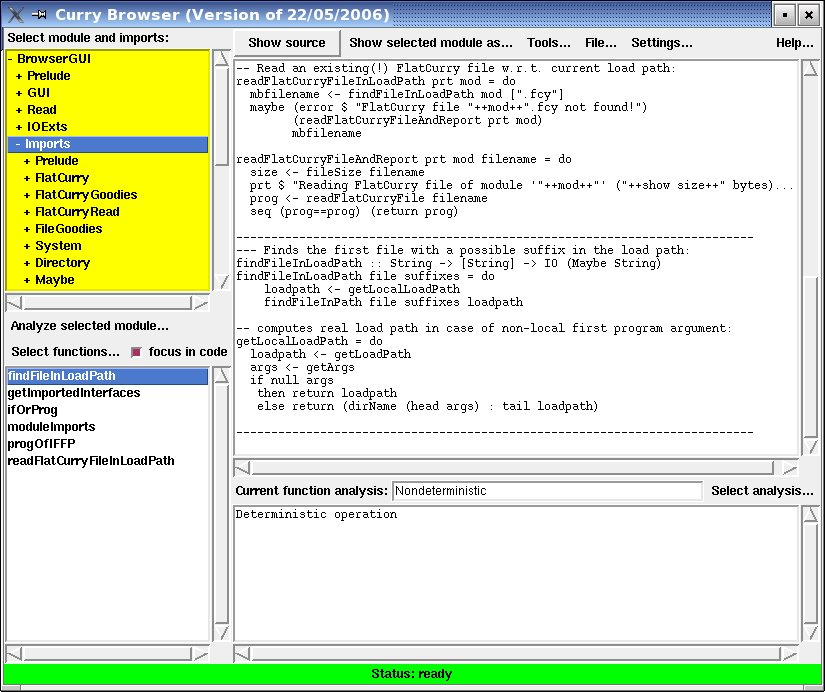
\includegraphics[scale=0.7]{currybrowser.jpg}
\end{center}
\caption{Snapshot of the main window of CurryBrowser\label{fig-currybrowser}}
\end{figure}
%
To get an impression of the use of \cb, Figure~\ref{fig-currybrowser}
shows a snapshot of its use on a particular application
(here: the implementation of \cb).
The upper list box in the left column shows the modules and their imports
in order to browse through the modules of an application.
Similarly to directory browsers, the list of imported modules of a module
can be opened or closed by clicking.
After selecting a module in the list of modules, its source code,
interface, or various other formats of the module can be shown
in the main (right) text area. For instance, one can show
pretty-printed versions of the intermediate flat programs (see below)
in order to see how local function definitions are translated by lambda lifting
\cite{Johnsson85}
or pattern matching is translated into case expressions \cite{Hanus97POPL,Wadler87}.
Since Curry is a language with parametric polymorphism and type inference,
programmers often omit the type signatures when defining functions.
Therefore, one can also view (and store) the selected module as source code where
missing type signatures are added.

Below the list box for selecting modules, there is a menu
(``Analyze selected module'') to analyze all functions
of the currently selected module at once. This is useful
to spot some functions of a module that could be problematic
in some application contexts, like functions that are impure (i.e., the result
depends on the evaluation time) or partially defined (i.e.,
not evaluable on all ground terms).
If such an analysis is selected,
the names of all functions are shown in the
lower list box of the left column (the ``function list'')
with prefixes indicating the properties of the individual functions.

The function list box can be also filled with functions
via the menu ``Select functions''. For instance, all functions
or only the exported functions defined in the currently selected
module can be shown there, or all functions from different modules
that are directly or indirectly called from
a currently selected function.
This list box is central to focus on a function in the
source code of some module or to analyze some function,
i.e., showing their properties. In order to focus on a function,
it is sufficient to check the ``focus on code'' button.
To analyze an individually selected function, one can
select an analysis from the list of available program analyses
(through the menu ``Select analysis'').
In this case, the analysis results are either shown
in the text box below the main text area
or visualized by separate tools, e.g., by a graph drawing tool for
visualizing call graphs.
Some analyses are local, i.e., they need only to consider the local definition
of this function (e.g., ``Calls directly,'' ``Overlapping rules,''
``Pattern completeness''),
where other analyses are global, i.e.,
they consider the definitions of all functions directly or indirectly called
by this function (e.g., ``Depends on,'' ``Solution complete,''
``Set-valued'').
%
Finally, there are a few additional tools integrated into \cb,
for instance, to visualize the import relation between all modules
as a dependency graph. These tools are available through the ``Tools'' menu.

More details about the use of \cb and all built-in analyses
are available through the ``Help'' menu of \cb.


\newpage

\section{CurryTest: A Tool for Testing Curry Programs}
\label{sec-currytest}

CurryTest\index{CurryTest}\index{testing programs}\index{program!testing}
is a simple tool in the PAKCS distribution to write
and run repeatable tests. CurryTest simplifies the task
of writing test cases for a module and executing them.
The tool is easy to use. Assume one has implemented a module \code{MyMod}
and wants to write some test cases to test its functionality,
making regression tests in future versions, etc.
For this purpose, there is a system library \code{Assertion}
(Section~\ref{Library:Assertion}) which
contains the necessary definitions for writing tests.
In particular, it exports an abstract polymorphic type \ccode{Assertion a}
together with the following operations:
\startprog
assertTrue      :: String -> Bool -> Assertion ()
assertEqual     :: String -> a -> a -> Assertion a
assertValues    :: String -> a -> [a] -> Assertion a
assertSolutions :: String -> (a->Success) -> [a] -> Assertion a
assertIO        :: String -> IO a -> a -> Assertion a
assertEqualIO   :: String -> IO a -> IO a -> Assertion a
\stopprog
The expression \ccode{assertTrue $s$ $b$}
is an assertion (named $s$) that the expression $b$ has the value \code{True}.
Similarly, the expression \ccode{assertEqual $s$ $e_1$ $e_2$}
asserts that the expressions $e_1$ and $e_2$
must be equal (i.e., \code{$e_1$==$e_2$} must hold),
the expression \ccode{assertValues $s$ $e$ $vs$} asserts
that $vs$ is the multiset of all values of $e$,
and the expression \ccode{assertSolutions $s$ $c$ $vs$} asserts
that the constraint abstraction $c$ has the multiset of solutions $vs$.
Furthermore, the expression \ccode{assertIO $s$ $a$ $v$}
asserts that the I/O action $a$ yields the value $v$ whenever it is
executed, and
the expression \ccode{assertEqualIO $s$ $a_1$ $a_2$}
asserts that the I/O actions $a_1$ and $a_2$ yields equal values.
The name $s$ provided as a first argument in each assertion
is used in the protocol produced by the test tool.

One can define a test program by importing the module
to be tested together with the module \code{Assertion} and defining
top-level functions of type \code{Assertion} in this module
(which must also be exported).
As an example, consider the following program
that can be used to test some list processing functions:
\startprog
\medskip
import List
import Assertion
\medskip
test1 = assertEqual     "++"     ([1,2]++[3,4]) [1,2,3,4]
\medskip
test2 = assertTrue      "all"    (all (<5) [1,2,3,4])
\medskip
test3 = assertSolutions "prefix" (\labs{}x -> let y free in  x\,++\,y =:= [1,2])
                                 [[],[1],[1,2]]
\medskip
\stopprog
For instance, \code{test1} asserts that the result of evaluating the
expression \code{([1,2]++[3,4])} is equal to \code{[1,2,3,4]}.

We can execute a test suite by the command\pindex{currytest}
\startprog
currytest testList
\stopprog
(\code{currytest} is a program stored in \code{$pakcshome$/bin}
where $pakcshome$ is the installation directory of PAKCS;
see Section~\ref{sec-general}).
In our example, \ccode{testList.curry} is the program containing the
definition of all assertions. This has the effect
that all exported top-level functions
of type \code{Assertion} are tested (i.e., the corresponding
assertions are checked) and the results
(\ccode{OK} or failure) are reported together with the name of each assertion.
%If failures occur, the complete test results are also
%written into a file named \ccode{testList.testlog}.''
For our example above, we obtain the following successful protocol:
\startprog
============================================================
Testing module "testList"...
OK: ++
OK: all
OK: prefix
All tests successfully passed.
============================================================
\stopprog
There is also a graphical interface that summarizes the results
more nicely.\footnote{Due to a bug in older versions of SICStus-Prolog,
it works only with SICStus-Prolog version 3.8.5 (or newer).}
In order to start this interface, one has to add the parameter
\ccode{--window} (or \ccode{-w}), e.g., executing a test suite by
\startprog
currytest --window testList
\stopprog
or
\startprog
currytest -w testList
\stopprog
A snapshot of the interface is shown in Figure~\ref{fig-currytest}.

\begin{figure}%[t]
\begin{center}
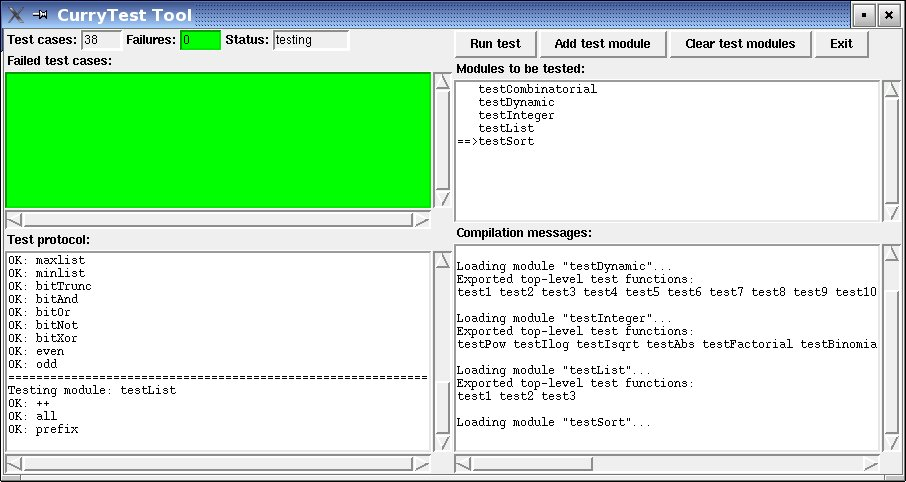
\includegraphics[scale=0.7]{currytest.jpg}
\end{center}
\caption{Snapshot of CurryTest's graphical interface\label{fig-currytest}}
\end{figure}


\newpage

\section{ERD2Curry: A Tool to Generate Programs from ER Specifications}
\label{sec-erd2curry}

ERD2Curry\index{ERD2Curry}\index{database programming}
is a tool to generate Curry code to access and manipulate data
persistently stored from
entity relationship diagrams.\index{entity relationship diagrams}
The idea of this tool is described in detail in
\cite{BrasselHanusMueller08PADL}.
Thus, we describe only the basic steps to use this tool
in the following.

If one creates an entity relationship diagram (ERD)
with the Umbrello UML Modeller, one has to store its
XML description in XMI format (as offered by Umbrello)
in a file, e.g., \ccode{myerd.xmi}.
This description can be compiled into a Curry program by the
command\pindex{erd2curry}
\startprog
erd2curry myerd.xmi
\stopprog
(\code{erd2curry} is a program stored in \code{$pakcshome$/bin}
where $pakcshome$ is the installation directory of PAKCS;
see Section~\ref{sec-general}).
If \code{MyData} is the name of the ERD, the Curry program file
\ccode{MyData.curry} is generated containing all the necessary
database access code as described in \cite{BrasselHanusMueller08PADL}.

If one does not want to use the Umbrello UML Modeller,
one can also create a textual description of the ERD
as a Curry term of type \code{ERD}
(w.r.t.\ the type definition given in module
\code{$pakcshome$/tools/erd2curry/ERD.curry})
and store it in some file, e.g., \ccode{myerd.term}.
This description can be compiled into a Curry program by the
command\pindex{erd2curry}
\startprog
erd2curry -t myerd.term
\stopprog
%
There is also the possibility to visualize an ERD term
as a graph with the graph visualization program \code{dotty}
(for this purpose, it might be necessary to adapt the definition
of the operation \code{dotCmd} in
\code{$pakcshome$/tools/erd2curry/ERD2Graph.curry}
according to your local environment).
This can be done by the command
\startprog
erd2curry -v myerd.term
\stopprog

\paragraph{Inclusion in the Curry application:}
To compile the generated database code, either
include the directory \code{$pakcshome$/tools/erd2curry}
into your Curry load path
(e.g., by setting  the environment variable
\ccode{CURRYPATH}\pindex{CURRYPATH}, see also Section~\ref{sec-modules})
or copy the file
\code{$pakcshome$/tools/erd2curry/ERDGeneric.curry}
into the directory of the generated database code.


\newpage

\section{UI: Declarative Programming of User Interfaces}
\label{sec-ui}

The PAKCS distribution contains a collection of libraries
to implement graphical user interfaces\index{user interface}
as well as web-based user interfaces
from declarative descriptions.
Exploiting these libraries, it is possible
to define the structure and functionality of a user interface
independent from the concrete technology.
Thus, a graphical user interface or a web-based user interface
can be generated from the same description by simply changing
the imported libraries.
This programming technique is described in detail in
\cite{HanusKluss09PADL}.

The libraries implementing these user interfaces are contained
in the directory
\startprog
$pakcshome$/tools/ui
\stopprog
Thus, in order to compile programs containing such user interface
specifications, one has to
include the directory \code{$pakcshome$/tools/ui}
into the Curry load path
(e.g., by setting  the environment variable
\ccode{CURRYPATH}\pindex{CURRYPATH}, see also Section~\ref{sec-modules}).
The directory
\startprog
$pakcshome$/tools/ui/examples
\stopprog
contains a few examples for such user interface specifications.


\newpage

\section{Preprocessing FlatCurry Files}
\label{sec-pakcspp}

The current parser allows to apply transformations on the intermediate
FlatCurry files after they are generated from the
corresponding Curry source file.
Currently, only the FlatCurry file corresponding to the main module
can be transformed.

A transformation can be specified as follows:
\begin{enumerate}
\item {\bf Options to \code{pakcs/bin/parsecurry}:}
\begin{description}
\item[\fbox{\code{--fpopt}}]\pindex{-fpopt}
Apply functional pattern optimization
(see \code{pakcs/tools/optimize/NonStrictOpt.curry} for details).

\item[\fbox{\code{--compact}}]\pindex{--compact}
Apply code compactification after parsing, i.e., transform the main
module and all its imported into one module and delete all
non-accessible functions.

\item[\fbox{\code{--compactexport}}]
Similar to \code{--compact} but delete all functions that are not accessible
from the exported functions of the main module.

\item[\fbox{\code{--compactmain:f}}]
Similar to \code{--compact} but delete all functions that are not accessible
from the function \ccode{f} of the main module.

\item[\fbox{\code{--fcypp cmd}}]\pindex{--fcypp}
Apply command \code{cmd} to the main module after parsing. This is useful to
integrate your own transformation into the compilation process.
Note that the command \ccode{cmd prog} should perform a transformation
on the FlatCurry file \code{prog.fcy}, i.e., it replaces the FlatCurry
file by a new one.
\end{description}

\item {\bf Setting the environment variable \code{FCYPP}:}\pindex{FCYPP}\\
For instance, setting \code{FCYPP} by
\startprog
export FCYPP="--fpopt"
\stopprog
will apply the functional pattern optimization if programs are compiled
and loaded in the PAKCS programming environment.


\item {\bf Putting options into the source code:}\pindex{PAKCS_OPTION_FCYPP}\\
If the source code contains a line with a comment of the form (the comment
must start at the beginning of the line)
\startprog
\{-\# PAKCS_OPTION_FCYPP <options> \#-\}
\stopprog
then the transformations specified by \code{<options>} are applied after
translating the source code into FlatCurry code. For instance,
the functional pattern optimization can be set by the comment
\startprog
\{-\# PAKCS_OPTION_FCYPP --fpopt \#-\}
\stopprog
in the source code. Note that this comment must be in a single line 
of the source program. If there are multiple lines containing such comments,
only the first one will be considered.
\end{enumerate}
\paragraph{Multiple options:}
Note that an arbitrary number of transformations can be specified
by the methods described above.
If several specifications for preprocessing FlatCurry files are used,
they are executed in the following order:
\begin{enumerate}
\item all transformations specified by the environemnt variable
\code{FCYPP} (from left to right)
\item all transformations specified as command line options of parsecurry
   (from left to right)
\item all transformations specified by a comment line in the source code
   (from left to right)
\end{enumerate}


\newpage

\section{Technical Problems}

Due to the fact that Curry is intended to implement
distributed systems (see Appendix~\ref{sec-ports}),
it might be possible that some technical problems
arise due to the use of sockets for implementing these
features. Therefore, this section gives some information
about the technical requirements of PAKCS and how to solve
problems due to these requirements.

There is one fixed port that is used by the implementation of PAKCS:
\begin{description}
\item[Port 8766:] This port is used by the
{\bf Curry Port Name Server} (CPNS) to implement symbolic names for
ports in Curry (see Appendix~\ref{sec-ports}).
If some other process uses this port on the machine,
the distribution facilities defined in the module \code{Ports}
(see Appendix~\ref{sec-ports}) cannot be used.
\end{description}
If these features do not work, you can try to find out
whether this port is in use by the shell command
\ccode{netstat -a | fgrep 8766} (or similar).

The CPNS is implemented as a demon listening on its port 8766
in order to serve requests about registering a new symbolic
name for a Curry port or asking the physical port number
of a Curry port. The demon will be automatically started for
the first time on a machine when a user compiles a program
using Curry ports. It can also be manually started and terminated by the
scripts \code{$pakcshome$/cpns/start} and
\code{$pakcshome$/cpns/stop}.
If the demon is already running, the command \code{$pakcshome$/cpns/start}
does nothing (so it can be always executed
before invoking a Curry program using ports).

If you detect any further technical problem,
please write to
\begin{center}
\code{mh@informatik.uni-kiel.de}
\end{center}

\newpage

\addcontentsline{toc}{section}{Bibliography}
\bibliography{manual}
\bibliographystyle{plain}

\newpage
\appendix

\section{Libraries of the PAKCS Distribution}
\label{sec:libraries}

{\setlength{\parindent}{0.0cm}

The PAKCS compiler system provides an extensive collection
of libraries for application programming.
The libraries for arithmetic constraints over real numbers,
finite domain constraints,
ports for concurrent and distributed programming, and
meta-programming by representing Curry programs in Curry
are described in the following subsection in more detail.
The complete set of libraries with all exported types and functions
are described in the further subsections.
For a more detailed online documentation of all libraries of PAKCS,
see \url{http://www.informatik.uni-kiel.de/~pakcs/lib/index.html}.

\subsection{Constraints, Ports, Meta-Programming}

\subsubsection{Arithmetic Constraints}

The primitive entities for the use of arithmetic constraints
are defined in the system module \code{CLPR}
(cf.\ Section~\ref{sec-modules}), i.e., in order to use them,
the program must contain the import declaration
\startprog
import CLPR
\stopprog
Floating point arithmetic is supported in PAKCS
via arithmetic constraints, i.e., the equational constraint
\ccode{2.3 +.~x =:= 5.5} is solved by binding \code{x} to \code{3.2}
(rather than suspending the evaluation of the addition,
as in corresponding constraints on integers like
\ccode{3+x=:=5}). All operations related to
floating point numbers are suffixed by \ccode{.}.
The following functions and constraints on floating point
numbers are supported in PAKCS:
\begin{description}
\item[\code{(+.)   :: Float -> Float -> Float}]~\\
Addition on floating point numbers.
\item[\code{(-.)   :: Float -> Float -> Float}]~\\
Subtraction on floating point numbers.
\item[\code{(*.)   :: Float -> Float -> Float}]~\\
Multiplication on floating point numbers.
\item[\code{(/.)   :: Float -> Float -> Float}]~\\
Division on floating point numbers.
\item[\code{(<.)   :: Float -> Float -> Success}]~\\
Comparing two floating point numbers with the ``less than'' relation.
\item[\code{(>.)   :: Float -> Float -> Success}]~\\
Comparing two floating point numbers with the ``greater than'' relation.
\item[\code{(<=.)  :: Float -> Float -> Success}]~\\
Comparing two floating point numbers with the ``less than or equal'' relation.
\item[\code{(>=.)  :: Float -> Float -> Success}]~\\
Comparing two floating point numbers with the ``greater than or equal''
relation.
\item[\code{i2f    :: Int -> Float}]~\\
Converting an integer number into a floating point number.
\end{description}
As an example, consider a constraint \code{mortgage}
which relates the principal \code{p},
the lifetime of the mortgage in months \code{t},
the monthly interest rate \code{ir},
the monthly repayment \code{r},
and the outstanding balance at the end of the lifetime \code{b}.
The financial calculations
can be defined by the following two rules in Curry (the second rule
describes the repeated accumulation of the interest):
\startprog
~
import CLPR
~
mortgage p t ir r b | t >. 0.0 \& t <=. 1.0  --lifetime not more than 1 month?
                    =  b =:= p *. (1.0 +. t *. ir) -. t*.r \vspace{1ex}
mortgage p t ir r b | t >. 1.0               --lifetime more than 1 month?
                    =  mortgage (p *. (1.0+.ir)-.r) (t-.1.0) ir r b
~
\stopprog
Then we can calculate the monthly payment for paying back
a loan of \$100,000 in 15 years with a monthly interest rate of 1\%
by solving the goal
\startprog
mortgage 100000.0 180.0 0.01 r 0.0
\stopprog
which yields the solution \code{r=1200.17}.

Note that only linear arithmetic equalities or inequalities
are solved by the constraint solver. Non-linear constraints
like \ccode{x *.~x =:= 4.0} are suspended until they become
linear.


\subsubsection{Finite Domain Constraints}

Finite domain constraints are constraints where all variables
can only take a finite number of possible values.
For simplicity, the domain of finite domain variables are
identified with a subset of the integers, i.e., the type
of a finite domain variable is \code{Int}. The arithmetic
operations related to finite domain variables are suffixed by \ccode{\#}.
The following functions and constraints for finite domain constraint solving
are currently supported in PAKCS:\footnote{Note that
this library is based on the corresponding library of SICStus-Prolog
but does not implement the complete functionality of the SICStus-Prolog library.
However, using the PAKCS interface for external functions (see
Appendix~\ref{sec-external-functions}), it is relatively
easy to provide the complete functionality.}

\begin{description}
\item[\code{domain :: [Int] -> Int -> Int -> Success}]~\\
The constraint \ccode{domain [$x_1,\ldots,x_n$] $l$ $u$}
is satisfied if the domain of all variables $x_i$ is the interval $[l,u]$.
\item[\code{(+\#)   :: Int -> Int -> Int}]~\\
Addition on finite domain values.
\item[\code{(-\#)   :: Int -> Int -> Int}]~\\
Subtraction on finite domain values.
\item[\code{(*\#)   :: Int -> Int -> Int}]~\\
Multiplication on finite domain values.
\item[\code{(=\#)   :: Int -> Int -> Success}]~\\
Equality of finite domain values.
\item[\code{(/=\#)  :: Int -> Int -> Success}]~\\
Disequality of finite domain values.
\item[\code{(<\#)   :: Int -> Int -> Success}]~\\
``less than'' relation on finite domain values.
\item[\code{(<=\#)  :: Int -> Int -> Success}]~\\
``less than or equal'' relation on finite domain values.
\item[\code{(>\#)   :: Int -> Int -> Success}]~\\
``greater than'' relation on finite domain values.
\item[\code{(>=\#)  :: Int -> Int -> Success}]~\\
``greater than or equal'' relation on finite domain values.
\item[\code{sum :: [Int] -> (Int -> Int -> Success) -> Int -> Success}]~\\
The constraint \ccode{sum [$x_1,\ldots,x_n$] $op$ $x$}
is satisfied if all $x_1+\cdots + x_n \mathrel{op} x$ is satisfied,
where $op$ is one of the above finite domain constraint relations
(e.g., \ccode{=\#}).
\item[\code{scalar_product :: [Int] -> [Int] -> (Int -> Int -> Success) -> Int -> Success}]~\\
The constraint \ccode{scalar_product [$c_1,\ldots,c_n$] [$x_1,\ldots,x_n$] $op$ $x$}
is satisfied if all $c_1 x_1+\cdots + c_n x_n \mathrel{op} x$ is satisfied,
where $op$ is one of the above finite domain constraint relations.
\item[\code{count :: Int -> [Int] -> (Int -> Int -> Success) -> Int -> Success}]~\\
The constraint \ccode{count $k$ [$x_1,\ldots,x_n$] $op$ $x$}
is satisfied if all $k \mathrel{op} x$ is satisfied,
where $n$ is the number of the $x_i$ that are equal to $k$ and
$op$ is one of the above finite domain constraint relations.
\item[\code{all_different :: [Int] -> Success}]~\\
The constraint \ccode{all_different [$x_1,\ldots,x_n$]}
is satisfied if all $x_i$ have pairwise different values.
\item[\code{labeling :: [LabelingOption] -> [Int] -> Success}]~\\
The constraint \ccode{labeling $os$ [$x_1,\ldots,x_n$]}
non-deterministically instantiates all $x_i$ to the values
of their domain according to the options $os$ (see the module documentation
for further details about these options).
\end{description}
These entities are defined in the system module \code{CLPFD}
(cf.\ Section~\ref{sec-modules}), i.e., in order to use it,
the program must contain the import declaration
\startprog
import CLPFD
\stopprog
As an example, consider the classical \ccode{send+more=money} problem
where each letter must be replaced by a different digit such that this
equation is valid and there are no leading zeros.
The usual way to solve finite domain constraint problems
is to specify the domain of the involved variables followed
by a specification of the constraints and the labeling
of the constraint variables in order to start the search for solutions.
Thus, the \ccode{send+more=money} problem can be solved as follows:
\startprog
~
import CLPFD
~
smm l =
        l =:= [s,e,n,d,m,o,r,y] \&
        domain l 0 9 \&
        s >\# 0 \&
        m >\# 0 \&
        all_different l  \&
                         1000 *\# s +\# 100 *\# e +\# 10 *\# n +\# d
        +\#               1000 *\# m +\# 100 *\# o +\# 10 *\# r +\# e
        =\# 10000 *\# m +\# 1000 *\# o +\# 100 *\# n +\# 10 *\# e +\# y \&
        labeling [FirstFail] l
        where s,e,n,d,m,o,r,y free
~
\stopprog
Then we can solve this problem by evaluating the goal
\ccode{smm [s,e,n,d,m,o,r,y]} which yields the unique solution
\code{\{s=9,e=5,n=6,d=7,m=1,o=0,r=8,y=2\}}.


\subsubsection{Ports: Distributed Programming in Curry}
\label{sec-ports}

To support the development of concurrent and distributed applications,
PAKCS supports internal and external ports\index{ports} as
described in \cite{Hanus99PPDP}.
Since \cite{Hanus99PPDP} contains a detailed description of this
concept together with various programming examples, we only summarize here
the functions and constraints supported for ports in PAKCS.

The basic datatypes, functions, and constraints for ports
are defined in the system module \code{Ports}
(cf.\ Section~\ref{sec-modules}), i.e., in order to use ports,
the program must contain the import declaration
\startprog
import Ports
\stopprog
This declaration includes the following entities in the program:
\begin{description}
\item[\code{Port a}\pindex{Port}]~\\
This is the datatype of a port to which one can send messages of type \code{a}.

\item[\code{openPort :: Port a -> [a] -> Success}]~\\
The constraint \ccode{openPort p s}\pindex{openPort}
establishes a new \emph{internal port}
\code{p} with an associated message stream \code{s}. \code{p} and \code{s} must be
unbound variables,
otherwise the constraint fails (and causes a runtime error).

\item[\code{send :: a -> Port a -> Success}]~\\
The constraint \ccode{send m p}\pindex{send}
is satisfied if \code{p} is constrained
to contain the message \code{m}, i.e., \code{m} will be sent to the port
\code{p} so that it appears in the corresponding stream.

\item[\code{doSend :: a -> Port a -> IO ()}]~\\
The I/O action \ccode{doSend m p}\pindex{doSend} solves the constraint
\ccode{send m p} and returns nothing.

\item[\code{openNamedPort :: String -> IO [a]}]~\\
The I/O action \ccode{openNamedPort n}\pindex{openNamedPort}
opens a new \emph{external port} with
symbolic name \code{n} and returns the associated stream of messages.

\item[\code{connectPort :: String -> IO (Port a)}]~\\
The I/O action \ccode{connectPort n}\pindex{connectPort}
returns a port with symbolic name
\code{n} (i.e., \code{n} must have the form ``\emph{portname@machine})
to which one can send messages by the \code{send} constraint.
Currently, no dynamic type checking is done for external ports,
i.e., sending messages of the wrong type to a port might lead to
a failure of the receiver.
\end{description}

\paragraph{Restrictions:}
Every expression, possibly containing logical variables, can be sent to
a port. However, as discussed in \cite{Hanus99PPDP},
port communication is strict, i.e., the expression is
evaluated to normal form before sending it by the
constraint \code{send}. Furthermore, if messages containing
logical variables are sent to \emph{external ports},
the behavior is as follows:
\begin{enumerate}
\item The sender waits until all logical variables in the message
have been bound by the receiver.
\item The binding of a logical variable received by a process
is sent back to the sender of this logical variable only if
it is bound to a \emph{ground} term, i.e., as long as the binding contains
logical variables, the sender is not informed about the binding
and, therefore, the sender waits.
\end{enumerate}

\paragraph{External ports on local machines:}
The implementation of external ports assumes that the
host machine running the application is connected to the Internet
(i.e., it uses the standard IP address of the host machine
for message sending). If this is not the case and the application
should be tested by using external ports only on the local host
without a connection to the Internet,
the environment variable \ccode{PAKCS_LOCALHOST}\pindex{PAKCS_LOCALHOST}
must be set to \ccode{yes}
\emph{before PAKCS system is started}.
In this case, the IP address \code{127.0.0.1} and the hostname
\ccode{localhost} are used for identifying the local machine.

\paragraph{Selection of Unix sockets for external ports:}
The implementation of ports uses sockets to communicate
messages sent to external ports.
Thus, if a Curry program uses the
I/O action \code{openNamedPort}\pindex{openNamedPort}
to establish an externally visible server,
PAKCS selects a Unix socket for the port communication.
Usually, a free socket is selected by the operating system.
If the socket number should be fixed in an application (e.g.,
because of the use of firewalls\index{firewall} that allow only
communication over particular sockets), then one
can set the environment variable \ccode{PAKCS_SOCKET}\pindex{PAKCS_SOCKET}
to a distinguished socket number before the PAKCS system is started.
This has the effect that PAKCS uses only this socket
number for communication (even for several external ports
used in the same application program).

\paragraph{Debugging:}
To debug distributed systems,
it is sometimes helpful to see all messages sent to external ports.
This is supported by the environment variable
\ccode{PAKCS_TRACEPORTS}.\pindex{PAKCS_TRACEPORTS}
If this variable is set to \ccode{yes}
\emph{before the PAKCS system is started}, then all
connections to external ports and all
messages sent and received on external ports are
printed on the standard error stream.


\subsubsection{AbstractCurry and FlatCurry: Meta-Programming in Curry}
\label{sec-flatcurry}

\index{AbstractCurry}
\index{FlatCurry}
To support meta-programming, i.e., the manipulation of Curry programs
in Curry, there are system modules \code{FlatCurry} and \code{AbstractCurry}
(stored in the directory \ccode{$pakcshome$/lib/meta})
which define datatypes for the representation
of Curry programs.
\code{AbstractCurry} is a more direct representation of a Curry program,
whereas \code{FlatCurry} is a simplified representation
where local function definitions are replaced by global definitions
(i.e., lambda lifting has been performed) and pattern matching
is translated into explicit case/or expressions.
Thus, \code{FlatCurry} can be used for more back-end oriented
program manipulations (or, for writing new back ends for Curry),
whereas \code{AbstractCurry} is intended for manipulations of
programs that are more oriented towards the source program.

Both modules contain predefined I/O actions to read programs
in the \code{AbstractCurry} (\code{readCurry}\pindex{readCurry})
or \code{FlatCurry}
(\code{readFlatCurry}\pindex{readFlatCurry}) format.
These actions parse the corresponding source program and return
a data term representing this program (according to the definitions
in the modules \code{AbstractCurry} and \code{FlatCurry}).

Since all datatypes are explained in detail in these modules,
we refer to the online documentation\footnote{%
\url{http://www.informatik.uni-kiel.de/~pakcs/lib/CDOC/FlatCurry.html} and
\url{http://www.informatik.uni-kiel.de/~pakcs/lib/CDOC/AbstractCurry.html}}
of these modules.

As an example, consider a program file \ccode{test.curry}
containing the following two lines:
\startprog
rev []     = []
rev (x:xs) = (rev xs) ++ [x]
\stopprog
Then the I/O action \code{(FlatCurry.readFlatCurry "test")} returns the
following term:
\startprog
 (Prog "test"
  ["Prelude"]
  []
  [Func ("test","rev") 1 Public
        (FuncType (TCons ("Prelude","[]") [(TVar 0)])
                  (TCons ("Prelude","[]") [(TVar 0)]))
        (Rule [0]
           (Case Flex (Var 0)
              [Branch (Pattern ("Prelude","[]") [])
                  (Comb ConsCall ("Prelude","[]") []),
               Branch (Pattern ("Prelude",":") [1,2])
                  (Comb FuncCall ("Prelude","++")
                        [Comb FuncCall ("test","rev") [Var 2],
                         Comb ConsCall ("Prelude",":")
                              [Var 1,Comb ConsCall ("Prelude","[]") []]
                        ])
              ]))]
  []
 )
\stopprog


%%%%%%%%%%%%%%%%%%%%%%%%%%%%%%%%%%%%%%%%%%%%%%%%%%%%%%%%%%%%%%%%%%%%%%%%%
% Definitions in order to LaTeX documents generated by "currydoc --tex"
%%%%%%%%%%%%%%%%%%%%%%%%%%%%%%%%%%%%%%%%%%%%%%%%%%%%%%%%%%%%%%%%%%%%%%%%%

\newcommand{\currymodule}[1]{\subsubsection{Library #1}\label{Library:#1}}
\newcommand{\currytypesstart}{\subsubsection*{Exported types:}}
\newcommand{\currytypesstop}{}
\newcommand{\currytypesynstart}[2]{{\tt type #2}\pindex{#1} \begin{quote}}
\newcommand{\currytypesynstop}{\end{quote}}
\newcommand{\currydatastart}[1]{{\tt data #1}\pindex{#1} \begin{quote}}
\newcommand{\currydatacons}{\end{quote}%
\begin{itemize}\item[] \hspace{-4ex}\emph{Exported constructors:}}
\newcommand{\currydatastop}{\end{itemize}}
\newcommand{\curryconsstart}[2]{\item {\tt #1~::~#2}\par}
\newcommand{\curryfuncstart}{\subsubsection*{Exported functions:}}
\newcommand{\curryfuncstop}{}
\newcommand{\curryfunctionstart}[2]{#2\pindex{#1}\begin{quote}}
\newcommand{\curryfunctionstop}{\end{quote}}
\newcommand{\curryfuncsig}[2]{{\tt #1~::~#2}}


\subsection{General Libraries}

\input{lib/AllSolutions}
\input{lib/Assertion}
\input{lib/Char}
\input{lib/CLPFD}
\input{lib/CLPR}
\input{lib/CLPB}
\input{lib/Combinatorial}
\input{lib/Constraint}
\input{lib/CSV}
\input{lib/Database}
\input{lib/DaVinci}
\input{lib/Directory}
\input{lib/Dynamic}
\input{lib/FileGoodies}
\input{lib/Float}
\input{lib/Global}
\input{lib/GlobalVariable}
\input{lib/GUI}
\input{lib/Integer}
\input{lib/IO}
\input{lib/IOExts}
\input{lib/JavaScript}
\input{lib/KeyDatabase}
\input{lib/KeyDatabaseSQLite}
\input{lib/KeyDB}
\input{lib/List}
\input{lib/Maybe}
\input{lib/NamedSocket}
\input{lib/Parser}
\input{lib/Ports}
\input{lib/Pretty}
\input{lib/Profile}
\input{lib/PropertyFile}
\input{lib/Read}
\input{lib/ReadNumeric}
\input{lib/ReadShowTerm}
\input{lib/SetFunctions}
\input{lib/Socket}
\input{lib/System}
\input{lib/Time}
%\input{lib/Tk}
\input{lib/Unsafe}


\subsection{Data Structures and Algorithms}

\input{lib/Array}
\input{lib/Dequeue}
\input{lib/FiniteMap}
\input{lib/GraphInductive}
\input{lib/Random}
\input{lib/RedBlackTree}
\input{lib/SetRBT}
\input{lib/Sort}
\input{lib/TableRBT}
\input{lib/Traversal}

\subsection{Libraries for Web Applications}

\input{lib/CategorizedHtmlList}
\input{lib/HTML}
\input{lib/HtmlParser}
\input{lib/Mail}
\input{lib/Markdown}
\input{lib/WUI}
\input{lib/URL}
\input{lib/XML}
\input{lib/XmlConv}

\subsection{Libraries for Meta-Programming}

\input{lib/AbstractCurry}
\input{lib/AbstractCurryPrinter}
\input{lib/CompactFlatCurry}
\input{lib/CurryStringClassifier}
\input{lib/FlatCurry}
\input{lib/FlatCurryGoodies}
\input{lib/FlatCurryRead}
\input{lib/FlatCurryShow}
\input{lib/FlatCurryTools}
\input{lib/FlatCurryXML}
\input{lib/FlexRigid}
\input{lib/PrettyAbstract}

} % end setlength parindent

\newpage

\input{markdown_syntax}

\newpage

\begin{figure}%[t]
\begin{center}
 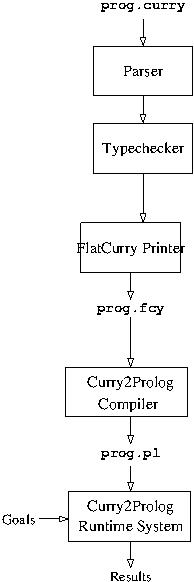
\includegraphics[scale=0.85]{pakcs_overview.jpg}
\end{center}\vspace{-5ex}
\caption{Overview of PAKCS\label{fig-pakcs}}
\end{figure}

\section{Overview of the PAKCS Distribution}

A schematic overview of the various components contained in
the distribution of PAKCS and the
translation process of programs inside PAKCS is shown in
Figure~\ref{fig-pakcs} on page~\pageref{fig-pakcs}.
In this figure, boxes denote different components of PAKCS
and names in boldface denote files containing
various intermediate representations during the translation
process (see Section~\ref{sec-auxfiles} below).
The PAKCS distribution contains a front end for reading (parsing and
type checking) Curry programs that can be also used by
other Curry implementations.
The back end (formerly known as ``Curry2Prolog''\index{Curry2Prolog})
compiles Curry programs into Prolog programs.
It also support constraint solvers for
arithmetic constraints over real numbers and finite domain constraints,
and further libraries for GUI programming, meta-programming etc.
Currently, it does not implement encapsulated search in full generality
(only a strict version of \code{findall} is supported),
and concurrent threads are not executed in a fair manner.


\newpage

\section{Auxiliary Files}
\label{sec-auxfiles}

During the translation and execution of a Curry program with PAKCS,
various intermediate representations of the source program are created
and stored in different files which are shortly explained in this section.
If you use the PAKCS, it is not necessary to know about
these auxiliary files because they are automatically generated
and updated. You should only remember the command for deleting
all auxiliary files (\ccode{cleancurry}, see Section~\ref{sec-general})
to clean up your directories.

The various components of PAKCS create
the following auxiliary files.
\begin{description}
\item[\code{prog.fcy}:] This file contains the Curry program
in the so-called ``FlatCurry'' representation where all functions are global
(i.e., lambda lifting has been performed) and pattern matching
is translated into explicit case/or expressions
(compare Appendix~\ref{sec-flatcurry}).
This representation might be useful for other back ends and
compilers for Curry and is the basis doing meta-programming in Curry.
This file is implicitly
generated when a program is read by PAKCS.
It can be also explicitly generated by the command\pindex{parsecurry}
\startprog
parsecurry --flat prog
\stopprog
The FlatCurry representation of a Curry program is usually
generated by the front-end after parsing, type checking and eliminating
local declarations.
If $dir$ is the directory where the Curry program is stored,
the corresponding FlatCurry program is stored in the directory
\ccode{$dir$/.curry}.

\item[\code{prog.fint}:] This file contains the interface
of the program in the so-called ``FlatCurry'' representation,
i.e., it is similar to \code{prog.fcy} but contains only exported
entities and the bodies of all functions omitted (i.e., ``external'').
This representation is useful for providing a fast access
to module interfaces.
This file is implicitly generated by the command\pindex{parsecurry}
\startprog
parsecurry --flat prog
\stopprog
and stored in the same directory as \code{prog.fcy}.

\item[\code{prog.pl}:] This file contains a Prolog program
as the result of translating the Curry program with PAKCS.
If $dir$ is the directory where the Curry program is stored,
the corresponding Prolog program is stored in the directory
\ccode{$dir$/.curry/.pakcs}.

\item[\code{prog.po}:] This file contains the Prolog program
\code{prog.pl} in an intermediate format for faster loading.
This file is stored in the same directory as \code{prog.pl}.

\item[\code{prog.state}:] This file contains the saved state
after compiling and saving a program with PAKCS
(see Section~\ref{sec-use-curry2prolog}).

\end{description}


\newpage


\section{Changing the Prelude or System Modules}

The standard prelude, which is automatically imported into each Curry program,
and all system modules containing datatypes and functions
useful for application programming
(cf.\ Appendix~\ref{sec:libraries})
are stored in the system module directory \ccode{$pakcshome$/lib}
(and its subdirectories).
If you change any of these modules,
you have to recompile the complete system by
executing \code{make} in the directory $pakcshome$.



\newpage

\section{External Functions}
\label{sec-external-functions}

\index{function!external}\index{external function}
Currently, PAKCS has no general interface to external functions.
Therefore, if a new external function should be added
to the system, this function must be declared as \code{external}
in the Curry source code
and then an implementation for this external function
must be inserted in the corresponding back end.
An external function is defined as follows in the Curry source code:
\begin{enumerate}
\item
Add a type declaration for the external function somewhere
in the body of the appropriate file (usually, the prelude
or some system module).
\item
For external functions it is not allowed to define any
rule since their semantics is determined by an external implementation.
Instead of the defining rules, you have to write
\startprog
f external
\stopprog
somewhere in the file containing the type declaration for 
the external function \code{f}.
\end{enumerate}
For instance, the addition on integers can be declared as
an external function as follows:
\startprog
(+) :: Int -> Int -> Int
(+) external
\stopprog
The further modifications to be done for an inclusion of
an external function has to be done in the back end.
A new external function is added to the back end of PAKCS
by informing the compiler about the existence of an external function
and adding an implementation of this function in the run-time
system. Therefore, the following items must be added
in the PAKCS compiler system:
\begin{enumerate}
\item
If the Curry module \code{Mod} contains external functions,
there must be a file named \code{Mod.prim_c2p} containing the
specification of these external functions. The contents of this file
is in XML format and has the following general structure:\footnote{%
\url{http://www.informatik.uni-kiel.de/~pakcs/primitives.dtd} contains a DTD
describing the exact structure of these files.}
\startprog
<primitives>
  \emph{specification of external function $f_1$}
  \ldots
  \emph{specification of external function $f_n$}
</primitives>
\stopprog
The specification of an external function $f$
with arity $n$ has the form
\startprog
<primitive name="$f$" arity="$n$">
  <library>lib</library>
  <entry>pred</entry>
</primitive>
\stopprog
where \code{lib} is the Prolog library (stored in the directory of the
Curry module or in the global directory
\code{$pakcshome$/curry2prolog/lib_src}) containing the code implementing this
function and \code{pred} is a predicate name in this library
implementing this function. Note that the function $f$ must be
declared in module \code{Mod}: either as an external function
or defined in Curry by equations. In the latter case,
the Curry definition is not translated but calls to this function
are redirected to the Prolog code specified above.

Furthermore, the list of specifications can also contain entries of the form
\startprog
<ignore name="$f$" arity="$n$" />
\stopprog
for functions $f$ with arity $n$ that are declared in module \code{Mod}
but should be ignored for code generation, e.g., since they are
never called w.r.t.\ to the current implementation of external functions.
For instance, this is useful when functions that can
be defined in Curry should be (usually more efficiently) are implemented
as external functions.

Note that the arguments are passed in their current (possibly unevaluated) form.
Thus, if the external function requires the arguments to be evaluated
in a particular form, this must be done before calling the external function.
For instance, the external function for adding two integers
requires that both arguments must be evaluated to non-variable head normal form
(which is identical to the ground constructor normal form). Therefore,
the function \ccode{+} is specified in the prelude by
\startprog
(+)   :: Int -> Int -> Int
x + y = (prim_Int_plus \$\# y) \$\# x
\medskip
prim_Int_plus :: Int -> Int -> Int
prim_Int_plus external
\stopprog
where \code{prim_Int_plus} is the actual external function implementing
the addition on integers. Consequently, the specification file
\code{Prelude.prim_c2p} has an entry of the form
\startprog
<primitive name="prim_Int_plus" arity="2">
  <library>prim_standard</library>
  <entry>prim_Int_plus</entry>
</primitive>
\stopprog
where the Prolog library \code{prim_standard.pl} contains the Prolog code
implementing this function.

\item
For most external functions, a \emph{standard interface} is
generated by the compiler so that an $n$-ary function can be
implemented by an $(n+1)$-ary predicate where the last argument must
be instantiated to the result of evaluating the function.  The
standard interface can be used if all arguments are ensured to be
fully evaluated (e.g., see definition of \code{(+)} above) and no
suspension control is necessary, i.e., it is ensured that the
external function call does not suspend for all arguments.
Otherwise, the raw interface (see below) must be used.  For
instance, the Prolog code implementing \code{prim_Int_plus}
contained in the Prolog library \code{prim_standard.pl} is as
follows (note that the arguments of \code{(+)} are passed in reverse
order to \code{prim_Int_plus} in order to ensure a left-to-right
evaluation of the original arguments by the calls to \code{(\$\#)}):
\startprog
prim_Int_plus(Y,X,R) :- R is X+Y.
\stopprog

\item
The \emph{standard interface for I/O actions}, i.e., external functions
with result type \code{IO~a}, assumes that the I/O action
is implemented as a predicate (with a possible side effect)
that instantiates the last argument to the returned value of type \ccode{a}.
For instance, the primitive predicate \code{prim_getChar}
implementing prelude I/O action \code{getChar}
can be implemented by the Prolog code
\startprog
prim_getChar(C) :- get_code(N), char_int(C,N).
\stopprog
where \code{char_int} is a predicate relating the internal
Curry representation of a character with its ASCII value.

\item
If some arguments passed to the external functions are not fully evaluated
or the external function might suspend, the implementation must follow
the structure of the PAKCS run-time system by using
the \emph{raw interface}. In this case, the name of the external entry
must be suffixed by \ccode{[raw]} in the \code{prim_c2p} file.
For instance, if we want to use the raw interface for the external function
\code{prim_Int_plus},
the specification file \code{Prelude.prim_c2p} must have an entry of the form
\startprog
<primitive name="prim_Int_plus" arity="2">
  <library>prim_standard</library>
  <entry>prim_Int_plus[raw]</entry>
</primitive>
\stopprog
In the raw interface, the actual implementation of an $n$-ary external function consists
of the definition of an $(n+3)$-ary predicate $pred$.
The first $n$ arguments are the corresponding actual arguments.
The $(n+1)$-th argument is a free variable which must be
instantiated to the result of the function call after
successful execution. The last two arguments
control the suspension behavior of the function
(see \cite{AntoyHanus00FROCOS} for more details):
The code for the predicate $pred$
should only be executed when the $(n+2)$-th argument
is not free, i.e., this predicate has always the
SICStus-Prolog block declaration
\startprog
?- block $pred$(?,\ldots,?,-,?).
\stopprog
In addition, typical external functions should suspend
until the actual arguments are instantiated. This can be ensured
by a call to \code{ensureNotFree} or \code{(\$\#)}
before calling the external function. Finally, the
last argument (which is a free variable at call time)
must be unified with the $(n+2)$-th argument
after the function call is successfully evaluated
(and does not suspend). Additionally, the actual (evaluated) arguments
must be dereferenced before they are accessed.
Thus, an implementation
of the external function for adding integers is as follows in the raw interface:
\startprog
?- block prim_Int_plus(?,?,?,-,?).
prim_Int_plus(RY,RX,Result,E0,E) :-
     deref(RX,X), deref(RY,Y), Result is X+Y, E0=E.
\stopprog
Here, \code{deref} is a predefined predicate for dereferencing the
actual argument into a constant (and \code{derefAll} for dereferencing
complex structures).
\end{enumerate}
%
The Prolog code implementing the external functions must be accessible to the run-time
system of PAKCS by putting it into the directory containing the corresponding
Curry module or into the system directory
\code{$pakcshome$/curry2prolog/lib_src}.
Then it will be automatically loaded into the run-time environment
of each compiled Curry program.

Note that arbitrary functions implemented in C or Java can be connected to
PAKCS by using the corresponding interfaces of underlying Prolog system.


\newpage
\addcontentsline{toc}{section}{Index}
\printindex


\end{document}

\clearpage
\documentclass[11pt,fleqn]{article}

\usepackage{latexsym}
\usepackage{makeidx}
\usepackage{url}
\usepackage{xspace}
\usepackage{graphicx}

\input{version}

%%% ------------------------------------------------------------------

\usepackage[colorlinks,linkcolor=blue]{hyperref}
\hypersetup{bookmarksopen=true}
\hypersetup{bookmarksopenlevel=0}
\hypersetup{pdftitle={PAKCS: The Portland Aachen Kiel Curry System}}
\hypersetup{pdfauthor={Michael Hanus}}
%\hypersetup{pdfstartview=Title}
\hypersetup{pdfstartview=FitH}
\usepackage{thumbpdf}

%%% ------------------------------------------------------------------

\setlength{\textwidth}{16.5cm}
\setlength{\textheight}{23cm}
\renewcommand{\baselinestretch}{1.1}
\setlength{\topmargin}{-1cm}
\setlength{\oddsidemargin}{0cm}
\setlength{\evensidemargin}{0cm}
\setlength{\marginparwidth}{0.0cm}
\setlength{\marginparsep}{0.0cm}

\newlength{\figurewidth}
\setlength{\figurewidth}{\textwidth}
\addtolength{\figurewidth}{-0.4cm}

% font for program texts
\renewcommand{\tt}{\usefont{OT1}{cmtt}{m}{n}\selectfont}
\newcommand{\codefont}{\tt}

% environment for typing program texts:
\makeatletter
\newenvironment{prog}{\par\vspace{0.7ex}
\setlength{\parindent}{1.0cm}
\setlength{\parskip}{-0.1ex}
\obeylines\@vobeyspaces\tt}{\vspace{0.7ex}\noindent
}
\makeatother
\newcommand{\startprog}{\begin{prog}}
\newcommand{\stopprog}{\end{prog}\noindent}

% program text in normal text
\newcommand{\code}[1]{\mbox{\codefont #1}}

% program text in normal text with apostrophs
\newcommand{\ccode}[1]{``\mbox{\codefont #1}''}

\newcommand{\pindex}[1]{\index{#1@{\tt #1}}}  % program elements in index

\newcommand{\labs}{\mbox{\tt\char92}}  % lambda abstraction in Curry
\newcommand{\todo}[1]{\fbox{\sc To do: #1}}
\newcommand{\cb}{CurryBrowser\xspace}

% allow underscores in programs:
\catcode`\_=\active
\let_=\sb
\catcode`\_=12

% produce an index:
\makeindex

\begin{document}
\sloppy

\begin{titlepage}
\pdfbookmark[1]{Title}{Title}
\begin{center}
\fbox{
\begin{minipage}[t]{\figurewidth}
\begin{center}\vspace{10ex}
{\Huge\bf PAKCS \pakcsversion}\\[4ex]
{\huge The Portland Aachen Kiel Curry System}\\[7ex]
{\huge User Manual}\\[4ex]
\pakcsversiondate\\[6ex]
\Large
Michael Hanus$^1$ [editor] \\[3ex]
{\large Additional Contributors:}\\[2ex]
Sergio Antoy$^2$ \\
Bernd Bra\ss{}el$^3$ \\
Martin Engelke$^4$ \\
Klaus H\"oppner$^5$ \\
Johannes Koj$^6$ \\
Philipp Niederau$^7$ \\
Ramin Sadre$^8$ \\
Frank Steiner$^9$ \\[4ex]
\normalsize
(1) University of Kiel, Germany, {\tt mh@informatik.uni-kiel.de} \\
(2) Portland State University, USA, {\tt antoy@cs.pdx.edu} \\
(3) University of Kiel, Germany, {\tt bbr@informatik.uni-kiel.de} \\
(4) University of Kiel, Germany, {\tt men@informatik.uni-kiel.de} \\
(5) University of Kiel, Germany, {\tt klh@informatik.uni-kiel.de} \\
(6) RWTH Aachen, Germany, {\tt johannes.koj@sdm.de} \\
(7) RWTH Aachen, Germany, {\tt philipp@navigium.de} \\
(8) RWTH Aachen, Germany, {\tt ramin@lvs.informatik.rwth-aachen.de} \\
(9) LMU Munich, Germany, {\tt fst@bio.informatik.uni-muenchen.de} \\[5ex]~
\end{center}
\end{minipage}}
\end{center}
\end{titlepage}

\pdfbookmark[1]{Contents}{Contents}
\tableofcontents

\newpage

\addcontentsline{toc}{section}{Preface}
\section*{Preface}

This document describes PAKCS (formerly called ``PACS''),
an implementation of the multi-paradigm language Curry,
jointly developed at the University of Kiel, the Technical University
of Aachen and Portland State University.
Curry is a universal programming language aiming at the amalgamation
of the most important declarative programming paradigms,
namely functional programming and logic programming.  
Curry combines in a seamless way features from functional programming
(nested expressions, lazy evaluation, higher-order functions),
logic programming (logical variables, partial data structures,
built-in search), and concurrent programming (concurrent evaluation
of constraints with synchronization on logical variables).
Moreover, the PAKCS implementation of Curry also supports
the high-level implementation of distributed applications,
graphical user interfaces, and web services
(as described in more detail in \cite{Hanus99PPDP,Hanus00PADL,Hanus01PADL}).

We assume familiarity with the ideas and features
of Curry as described in the Curry language definition \cite{Hanus12Curry}.
Therefore, this document only explains the use of the different
components of PAKCS
and the differences and restrictions of PAKCS
(see Section~\ref{sec-restrictions})
compared with the language Curry (Version 0.8.3).


\bigskip

\subsection*{Acknowledgements}

This work has been supported in part by the DAAD/NSF grant INT-9981317,
the NSF grants CCR-0110496 and CCR-0218224,
the Acci\'on Integrada hispano-alemana HA1997-0073,
and the DFG grants Ha 2457/1-2, Ha 2457/5-1, and Ha 2457/5-2.

Many thanks to the users of PAKCS for bug reports, bug fixes, and improvements,
in particular, to Marco Comini, Sebastian Fischer, Massimo Forni,
Carsten Heine, Stefan Junge, Frank Huch, Parissa Sadeghi.


\newpage

\section{Overview of PAKCS}

\subsection{General Use}
\label{sec-general}

This version of PAKCS has been tested on Sun Solaris, Linux, and Mac OS X
systems. In principle, it should be also executable on other
platforms on which a Prolog system like SICStus-Prolog or SWI-Prolog exists
(see the file \code{INSTALL.html} in the PAKCS directory
for a description of the necessary software to install PAKCS).

All executable files required to use the different components
of PAKCS are stored in the directory \code{$pakcshome$/bin}
(where $pakcshome$ is the installation directory of the complete
PAKCS installation). You should add this directory
to your path (e.g., by the \code{bash} command
\ccode{export PATH=$pakcshome$/bin:\$PATH}).

The source code of the Curry program
must be stored in a file with the suffix \ccode{.curry},
e.g., \code{prog.curry}. 
Literate programs must be stored in files with the extension \ccode{.lcurry}.
They are automatically converted into corresponding
\ccode{.curry} files by deleting all lines not starting 
with \ccode{>} and removing the prefix \ccode{> } of the
remaining lines.

Since the translation of Curry programs with PAKCS creates
some auxiliary files (see Section~\ref{sec-auxfiles} for details),
you need write permission
in the directory where you have stored your Curry programs.
The auxiliary files for all Curry programs in the current
directory can be deleted by the command\pindex{cleancurry}
\startprog
cleancurry
\stopprog
(this is a shell script stored in the \code{bin} directory of the
PAKCS installation, see above).
The command
\startprog
cleancurry -r
\stopprog
also deletes the auxiliary files in all subdirectories.



\subsection{Restrictions on Curry Programs}
\label{sec-restrictions}

There are a few minor restrictions on Curry programs
when they are processed with PAKCS:
\begin{itemize}
\item
\index{singleton variables}\index{variables!singleton}
\emph{Singleton pattern variables}, i.e., variables that occur only once
in a pattern of the rule, should be denoted as an anonymous variable \ccode{_},
otherwise the parser will print a warning since this is a
typical source of programming errors.
\item
PAKCS translates all \emph{local declarations} into global functions with
additional arguments (``lambda lifting'', see Appendix~D of the
Curry language report).
Thus, in the various run-time systems, the definition of
functions with local declarations look different from
their original definition (in order to see the result
of this transformation, you can use the \cb, see
Section~\ref{sec-currybrowser}).
\item \index{tabulator stops}
Tabulator stops instead of blank spaces in source files are
interpreted as stops at columns 9, 17, 25, 33, and so on.
\item Threads created by a concurrent conjunction are not executed
in a fair manner (usually, threads corresponding to leftmost constraints
are executed with higher priority).
\item
Encapsulated search\index{encapsulated search}: In order
to allow the integration of non-deterministic computations
in programs performing I/O at the top-level, PAKCS supports
the search operators \code{findall}\pindex{findall}
and \code{findfirst}\pindex{findfirst}.
In contrast to the general definition of encapsulated search
\cite{HanusSteiner98PLILP}, the current implementation suspends
the evaluation of \code{findall} and \code{findfirst}
until the argument does not contain unbound global variables.
Moreover, the evaluation of \code{findall} is strict,
i.e., it computes all solutions before returning the
complete list of solutions.
It is recommended to use the system module \code{AllSolutions}
for encapsulating search.
\item
There is currently no general connection to external constraint solvers.
However, the PAKCS compiler provides constraint
solvers for arithmetic and finite domain constraints
(see Appendix~\ref{sec:libraries}).
\end{itemize}

% Layout rule:
% (from Sergio's email of June 2, 1998)
%This is the general rule.  There are two kinds of syntactic
%constructs that rely on the offside rule.  One kind has a keyword
%indicating the end of the construct.  "let ... in" is the only
%representative of this kind.  Upon recognition of the keyword
%"in", all the constructs relying on the offide rule nested within
%the "let...in" are closed.  The other kind has no closing keyword.
%"where" and "choice" are the only constructs of this kind.
%Constructs of this kind can be closed only by indentation.  Any
%line, including a comment, indented less that the construct
%terminates it.  The indentation of "where", "choice" and "let" is
%the indentation of the first token following the keyword of the
%construct.
%



\subsection{Modules in PAKCS}
\label{sec-modules}

The current implementation of PAKCS supports only flat module names,
i.e., the notation \code{Dir.Mod.f} is not supported.\index{modules}
In order to allow the structuring of modules in different directories,
PAKCS searches for imported modules in various directories.
By default, imported modules are searched in the directory
of the main program and the system module directories
\ccode{$pakcshome$/lib} and \ccode{$pakcshome$/lib/meta}.
This search path can be extended
by setting the environment variable \code{CURRYPATH}\pindex{CURRYPATH}
(which can be also set in a PAKCS session by the command
\ccode{:set path}\pindex{path}\pindex{:set path},
see below)
to a list of directory names separated by colons (\ccode{:}).
In addition, a local standard search path
can be defined in the \ccode{.pakcsrc} file
(see Section~\ref{sec-customization}).
Thus, modules to be loaded are searched in the following
directories (in this order, i.e., the first occurrence of a module file
in this search path is imported):
\begin{enumerate}
\item Current working directory (\ccode{.}) or directory prefix
of the main module (e.g., directory \ccode{/home/joe/curryprogs}
if one loads the Curry program \ccode{/home/joe/curryprogs/main}).
\item The directories enumerated in the environment variable \code{CURRYPATH}.
\item The directories enumerated in the \ccode{.pakcsrc} variable
      \ccode{libraries}.
\item The directories \ccode{$pakcshome$/lib} and \ccode{$pakcshome$/lib/meta}.
\end{enumerate}
Note that the standard prelude (\code{$pakcshome$/lib/Prelude.curry})
will be always implicitly imported to all modules if a module
does not contain an explicit import declaration for the module
\code{Prelude}.


\newpage

\section{PAKCS: An Interactive Curry Development System}
\label{sec-curry2prolog}

PAKCS\index{PAKCS},
in the following just called ``PAKCS'',
is an interactive system to develop applications
written in Curry.
It is implemented in Prolog and compiles
Curry programs into Prolog programs. It contains various tools,
a source-level debugger,
solvers for arithmetic constraints over real numbers
and finite domain constraints, etc. The compilation process and the
execution of compiled programs is fairly efficient
if a good Prolog implementation like SICStus-Prolog is used.


\subsection{How to Use PAKCS}
\label{sec-use-curry2prolog}

To start PAKCS, execute the command
\ccode{pakcs}\pindex{pakcs}
(this is a shell script stored in
\code{$pakcshome$/bin} where $pakcshome$ is the installation directory
of PAKCS).
When the system is ready, the prelude (\code{$pakcshome$/lib/Prelude.curry})
is already loaded, i.e., all definitions in the prelude are accessible.
Now you can type in various commands.
The {\bf most important commands} are
(it is sufficient to type a unique prefix of a command if it is unique,
e.g., one can type \ccode{:r} instead of \ccode{:reload}):

\begin{description}
\item[\fbox{\code{:help}}]\pindex{:help}
Show a list of all available commands.

\item[\fbox{\code{:load $prog$}}]\pindex{:load}
Compile and load the program stored in \code{$prog$.curry}
together with all its imported modules.
If this file does not exist, the system looks for a FlatCurry
file \code{$prog$.fcy} and compiles from this intermediate representation.
If the file \code{$prog$.fcy} does not exists, too, the system looks
for a file \code{$prog$_flat.xml} containing a FlatCurry program in
XML representation (compare command \ccode{:xml}\pindex{:xml}),
translates this into a FlatCurry file \code{$prog$.fcy}
and compiles from this intermediate representation.

\item[\fbox{\code{:reload}}]\pindex{:reload}
Recompile all currently loaded modules.

\item[\fbox{\code{:add} $m$}]\pindex{:add}
Add module $m$ to the set of currently loaded modules
so that its exported entities are available in the top-level environment.

\item[\fbox{$expr$}] Evaluate the expression $expr$ to normal form
and show the computed results. Since the PAKCS
compiles Curry programs into Prolog programs,
non-deterministic computations are implemented by backtracking.
Therefore, computed results are shown one after the other.
After each computed result, you will be asked whether
you want to see the next alternative result or all alternative results.
The default answer value for this question can be defined
in the \ccode{.pakcsrc} file (see Section~\ref{sec-customization}).

\textbf{Free variables in initial expressions} must be declared as in Curry programs
(if the free variable mode\index{free variable mode} is not turned on,
see option \ccode{+free} below), i.e.,
either by a \ccode{let\ldots{}free in}
or by a \ccode{where\ldots{}free} declaration.
For instance, one can write
\startprog
let xs,ys free in xs++ys\,=:=\,[1,2]
\stopprog
or
\startprog
xs++ys\,=:=\,[1,2]  where xs,ys free
\stopprog
Without these declarations, an error is reported in order to
avoid the unintended introduction of free variables in initial expressions
by typos.

Note that lambda abstractions, \code{let}s and list comprehensions
in top-level expressions are not yet supported in initial expressions
typed in the top-level of PAKCS.

\item[\fbox{\code{let} $x$ \code{=} $expr$}]
Define the identifier $x$ as an abbreviation for the expression $expr$
which can be used in subsequent expressions. The identifier $x$
is visible until the next \code{load} or \code{reload} command.

\item[\fbox{\code{:quit}}]\pindex{:quit} Exit the system.
\end{description}
%
\bigskip
%
There are also a number of {\bf further commands} that are often
useful:
%
\begin{description}
\item[\fbox{\code{:type $expr$}}]\pindex{:type}
Show the type of the expression $expr$.

\item[\fbox{\code{:analyze}}]\pindex{:analyze}
Analyze the currently loaded program for some properties.
Currently, there are the following analysis options:
\begin{description}
\item[\fbox{\code{functions}}]
Check properties of all functions defined
in the currently loaded Curry program (i.e., without the functions defined
in the prelude and imported modules).
Currently, the following properties are checked:
\begin{enumerate}
\item Which functions are defined by overlapping left-hand sides?
\item Which functions are indeterministic, i.e., contains an
      indirect/implicit call to a \code{send} constraint on ports
      (see Appendix~\ref{sec-ports}, which includes
      an implicit committed choice)?
\end{enumerate}
\item[\fbox{\code{icalls}}]
Show all calls to imported functions in the currently loaded module.
This might be useful to see which import declarations are really necessary.
\end{description}

\item[\fbox{\code{:browse}}]\pindex{:browse}
Start the CurryBrowser to analyze the currently loaded
module together with all its imported modules
(see Section~\ref{sec-currybrowser} for more details).

\item[\fbox{\code{:edit}}]\pindex{:edit}
Load the source code of the current main module into a text editor.
If the environment variable \ccode{EDITOR} is set,
the value of this environment variable is used as the editor program,
otherwise a default editor (e.g., \ccode{vi}) is used.

\item[\fbox{\code{:edit $file$}}]\pindex{:edit}
Load file $file$ into a text editor which is defined
as in the command \ccode{:edit}.

\item[\fbox{\code{:interface}}]\pindex{:interface}
Show the interface of the currently loaded
module, i.e., show the names of all imported modules,
the fixity declarations of all exported operators,
the exported datatypes declarations and the types
of all exported functions.

\item[\fbox{\code{:interface $prog$}}]\pindex{:interface}
Similar to \ccode{:interface}
but shows the interface of the module \ccode{$prog$.curry}.
If this module does not exist, this command looks in the
system library directory of PAKCS for a module with this name,
e.g., the command \ccode{:interface FlatCurry} shows the interface
of the system module \code{FlatCurry} for meta-programming
(see Appendix~\ref{sec-flatcurry}).

\item[\fbox{\code{:modules}}]\pindex{:modules}
Show the list of all currently loaded modules.

\item[\fbox{\code{:programs}}]\pindex{:programs}
Show the list of all Curry programs that are available in the load path.

\item[\fbox{\code{:set $option$}}]\pindex{:set}
Set or turn on/off a specific option
of the PAKCS environment. Options are turned on by the prefix
\ccode{+} and off by the prefix \ccode{-}. Options that can only
be set (e.g., \code{printdepth}) must not contain a prefix.
The following options are currently supported:

\begin{description}
\item[\fbox{\code{+/-debug}}]\pindex{debug} Debug mode.
\index{debug mode}
In the debug mode, one can trace the evaluation of an expression,
setting spy points (break points) etc.\ (see the commands
for the debug mode described below).

\item[\fbox{\code{+/-free}}]\pindex{free} Free variable mode.\index{free variable mode}
If the free variable mode is off (default), then
free variables occurring in initial expressions entered in the
PAKCS environment must always be declared by a \ccode{let\ldots{}free in}
or \ccode{where\ldots{}free} declaration (as in Curry programs).
This avoids the introduction of free variables in initial expressions
by typos (which might lead to the exploration of infinite search spaces).
If the free variable mode is on, each undefined symbol
in an initial expression is considered as a free variable.

\item[\fbox{\code{+/-printfail}}]\pindex{printfail} Print failures.
If this option is set, failures occurring during evaluation
(i.e., non-reducible demanded subexpressions) are printed.
This is useful to see failed reductions due to partially
defined functions or failed unifications.
Inside encapsulated search (e.g., inside evaluations of
\code{findall} and \code{findfirst}), failures are not printed
(since they are a typical programming technique there).
Note that this option causes some overhead in execution time
and memory so that it could not be used in larger applications.

\item[\fbox{\code{+/-allfails}}]\pindex{allfails}
If this option is set, \emph{all} failures
(i.e., also failures on backtracking and failures
of enclosing functions that fail due to the failure of an argument
evaluation) are printed if the option \code{printfail} is set.
Otherwise, only the first failure (i.e., the first non-reducible
subexpression) is printed.

\item[\fbox{\code{+/-consfail}}]\pindex{consfail} Print constructor failures.
If this option is set, failures due to application of
functions with non-exhaustive pattern matching or failures
during unification (application of \ccode{=:=}) are shown.
Inside encapsulated search (e.g., inside evaluations of
\code{findall} and \code{findfirst}), failures are not printed
(since they are a typical programming technique there).
In contrast to the option \code{printfail},
this option creates only a small overhead in execution time
and memory use.

\item[\fbox{\code{+consfail all}}]\pindex{consfail}
Similarly to \ccode{+consfail}, but the complete trace
of all active (and just failed) function calls from the main function
to the failed function are shown.

\item[\fbox{\code{+consfail file:$f$}}]\pindex{consfail}
Similarly to \ccode{+consfail all}, but the complete fail trace
is stored in the file $f$. This option is useful in non-interactive
program executions like web scripts.

\item[\fbox{\code{+consfail int}}]\pindex{consfail}
Similarly to \ccode{+consfail all}, but after each failure occurrence,
an interactive mode for exploring the fail trace is started
(see help information in this interactive mode).
When the interactive mode is finished, the program execution
proceeds with a failure.

\item[\fbox{\code{+/-compact}}]\pindex{compact}
Reduce the size of target programs by using the
parser option \ccode{--compact}
(see Section~\ref{sec-pakcspp} for details about this option).

\item[\fbox{\code{+/-profile}}]\pindex{profile} Profile mode.
If the profile mode is on, then information about
the number of calls, failures, exits etc.\ are collected for
each function during the debug mode (see above) and shown
after the complete execution (additionaly, the result is stored
in the file \code{$prog$.profile} where $prog$ is the current main program).
The profile mode has no effect outside the debug mode.


\item[\fbox{\code{+/-suspend}}] Suspend mode (initially, it is off).
If the suspend mode is on, all suspended expressions
(if there are any) are shown (in their internal representation) at the end
of a computation.

\item[\fbox{\code{+/-time}}]\pindex{time} Time mode. If the time mode is on,
the cpu time and the elapsed time
of the computation is always printed together with the result
of an evaluation.

\item[\fbox{\code{+/-verbose}}] Verbose mode (initially, it is off).
If the verbose mode is on,
the initial expression of a computation (together with its type)
is printed before this expression is evaluated.

\item[\fbox{\code{+/-warn}}]\pindex{warn} Parser warnings. If the parser
warnings are turned on (default), the parser will print
warnings about variables that occur only once in a program rule
(see Section~\ref{sec-restrictions})
or locally declared names that shadow the definition of
globally declared names. If the parser warnings are switched off,
these warnings are not printed during the reading of a Curry program.

\item[\fbox{\code{path $path$}}]\pindex{path} Set the additional search path
for loading modules to $path$.
Note that this search path is only used for loading modules
inside this invocation of PAKCS, i.e., the environment variable
\ccode{CURRYPATH}\pindex{CURRYPATH} (see also Section~\ref{sec-modules})
is set to $path$ in this invocation of PAKCS.

\item[\fbox{\code{printdepth $n$}}]\pindex{printdepth}
Set the depth for printing terms to the value \code{n} (initially: 10).
In this case subterms with a depth greater than \code{n} are abbreviated
by dots when they are printed as a result of a computation
or during debugging. A value of \code{0} means infinite depth
so that the complete terms are printed.

\end{description}

\item[\fbox{\code{:set}}]\pindex{:set}
Show a help text on the \ccode{:set $option$}
command together with the current values of all options.

\item[\fbox{\code{:show}}]\pindex{:show}
Show the source text of the currently loaded Curry program.
If the environment variable \code{PAGER} is defined,
use its value to show the program, other use the command \ccode{more}.
If the source text is not available
(since the program has been directly compiled from a FlatCurry
or XML file), the loaded program is decompiled and
the decompiled Curry program text is shown.

\item[\fbox{\code{:show $m$}}]\pindex{:show}
Show the source text of module $m$ which must be accessible
via the current load path.

\item[\fbox{\code{:show $f$}}]\pindex{:show}
Show the source code of function $f$ (provided that the name $f$
is different from a module accessilbe via the current load path)
in a separate window.

\item[\fbox{\code{:cd $dir$}}]\pindex{:cd}
Change the current working directory to $dir$.

\item[\fbox{\code{:dir}}]\pindex{:dir} Show the names of all Curry programs
in the current working directory.

\item[\fbox{\code{:!$cmd$}}]\pindex{:"!} Shell escape: execute $cmd$ in a Unix shell.

\item[\fbox{\code{:save}}]\pindex{:save} Save the current state of the system
(together with the compiled program \code{prog.curry}) in the file
\code{prog.state}, i.e., you can later start the program again
by typing \ccode{prog.state} as a Unix command.

\item[\fbox{\code{:save $expr$}}]\pindex{:save} Similar as \ccode{:save}
but the expression $expr$ (typically: a call to the main
function) will be executed after restoring the state
and the execution of the restored state terminates when
the evaluation of the expression $expr$ terminates.

\item[\fbox{\code{:fork $expr$}}]\pindex{:fork}
The expression $expr$, which must be of type \ccode{IO ()},
is evaluated in an independent process which runs in
parallel to the current PAKCS process.
All output and error messages from this new process are suppressed.
This command is useful to test distributed Curry programs
(see Appendix~\ref{sec-ports}) where one can start
a new server process by this command. The new process
will be terminated when the evaluation of the expression $expr$
is finished.

\item[\fbox{\code{:coosy}}]\pindex{:coosy}
Start the Curry Object Observation System COOSy,
a tool to observe the execution of Curry programs.
This commands starts a graphical user interface to show
the observation results and adds to the load path the directory
containing the modules that must be imported in order to annotate
a program with observation points.
Details about the use of COOSy can be found in the
COOSy interface (under the ``Info'' button), and details
about the general idea of observation debugging and the implementation
of COOSy can be found in \cite{BrasselChitilHanusHuch04PADL}.

\item[\fbox{\code{:xml}}]\pindex{:xml}
Translate the currently loaded program module into an XML representation
according to the format described in
\url{http://www.informatik.uni-kiel.de/~curry/flat/}.
Actually, this yields an implementation-independent
representation of the corresponding FlatCurry program
(see Appendix~\ref{sec-flatcurry} for a description of FlatCurry).
If $prog$ is the name of the currently loaded program,
the XML representation will be written into the file \ccode{$prog$_flat.xml}.

\item[\fbox{\code{:peval}}]\pindex{:peval}
Translate the currently loaded program module into an equivalent
program where some subexpressions are partially evaluated
so that these subexpressions are (hopefully) more efficiently executed.
An expression $e$ to be partially evaluated
must be marked in the source program by \code{(PEVAL e)}
(where \code{PEVAL} is defined as the identity function in the prelude
so that it has no semantical meaning).

The partial evaluator
translates a source program \code{$prog$.curry} into the
partially evaluated program in intermediate representation
stored in \code{$prog$_pe.fcy}. The latter program is implicitly loaded
by the \code{peval} command so that the partially evaluated program
is directly available. The corresponding source program
can be shown by the \code{show} command (see above).

The current partial evaluator is an experimental prototype
(so it might not work on all programs) based on the ideas
described in \cite{AlbertAlpuenteHanusVidal99LPAR,AlbertHanusVidal00LPAR,%
AlbertHanusVidal01FLOPS,AlbertHanusVidal02JFLP}.

\end{description}
%
\bigskip
%
PAKCS can also execute programs in the {\bf debug mode}.
\index{debug mode}\pindex{debug}
The debug mode is switched on by setting the \code{debug} option
with the command \ccode{:set +debug}. In order to switch
back to normal evaluation of the program, one has to execute
the command \ccode{:set -debug}.

In the debug mode, PAKCS offers the following
{\bf additional options for the \ccode{:set} command:}
%
\begin{description}
\item[\fbox{\code{+/-single}}]\pindex{single}
Turn on/off single mode for debugging.
If the single mode is on, the evaluation of an expression
is stopped after each step and the user is asked how to proceed
(see the options there).

\item[\fbox{\code{+/-trace}}]\pindex{trace}
Turn on/off trace mode for debugging.
If the trace mode is on, all intermediate expressions occurring
during the evaluation of an expressions are shown.

\item[\fbox{\code{spy $f$}}]\pindex{spy}
Set a spy point (break point) on the
function $f$. In the single mode, you can ``leap'' from spy point
to spy point (see the options shown in the single mode).

\item[\fbox{\code{+/-spy}}]\pindex{spy} Turn on/off spy mode for debugging.
If the spy mode is on, the single mode is automatically activated
when a spy point is reached.
\end{description}


\subsection{Command Line Editing}

In order to have support for line editing or history functionality
in the command line of PAKCS (as often supported by the \code{readline}
library), you should have the Unix command \code{rlwrap} installed
on your local machine.
If \code{rlwrap} is installed, it is used by PAKCS if called on a terminal.
If it should not be used (e.g., because it is executed
in an editor with \code{readline} functionality), one can
call PAKCS with the parameter \ccode{--noreadline}.


\subsection{Customization}
\label{sec-customization}

In order to customize the behavior of PAKCS to your own preferences,
there is a configuration file which is read by PAKCS when it is invoked.
When you start PAKCS for the first time, a standard version of
this configuration file is copied with the name
\ccode{.pakcsrc}\pindex{pakcsrc}\pindex{.pakcsrc}
into your home directory. The file contains definitions
of various settings, e.g., about showing warnings, progress messages etc.
After you have started PAKCS for the first time, look into this file
and adapt it to your own preferences.


\subsection{Emacs Interface}

Emacs is a powerful programmable editor suitable for program development.
It is freely available for many platforms
(see \url{http://www.emacs.org} or \url{http://www.xemacs.org}).
The distribution of PAKCS contains also a special
\emph{Curry mode}\index{Curry mode}\index{Emacs}
that supports the development of Curry programs in
the (X)Emacs environment.
This mode includes support for syntax highlighting,
finding declarations in the current buffer, and
loading Curry programs into the PAKCS compiler system
in an Emacs shell.

The Curry mode has been adapted from a similar mode for Haskell programs.
Its installation is described in the file \code{README}
in directory \ccode{$pakcshome$/tools/emacs} which also contains
the sources of the Curry mode and a short description about
the use of this mode.


\newpage

\section{Extensions}
\label{sec-extensions}

PAKCS supports some extensions in Curry programs that are not (yet)
part of the definition of Curry. These extensions are described below.

\subsection{Recursive Variable Bindings}

Local variable declarations (introduced by \code{let}\pindex{let}
or \code{where}\pindex{where}) can be (mutually) recursive in PAKCS.
For instance, the declaration
\startprog
ones5 = let ones = 1 : ones
         in take 5 ones
\stopprog
introduces the local variable \code{ones} which is bound
to a \emph{cyclic structure}\index{cyclic structure}
representing an infinite list of \code{1}'s.
Similarly, the definition
\startprog
onetwo n = take n one2
 where
   one2 = 1 : two1
   two1 = 2 : one2
\stopprog
introduces a local variables \code{one2} that represents
an infinite list of alternating \code{1}'s and \code{2}'s
so that the expression \code{(onetwo 6)} evaluates to \code{[1,2,1,2,1,2]}.


\subsection{Functional Patterns}

Functional patterns \cite{AntoyHanus05LOPSTR} are a useful extension
to code operations in a more readable way. Furthermore,
defining operations with functional patterns avoids problems
caused by strict equality (\ccode{=:=}) and leads to programs
that are potentially more efficient.

Consider the definition of an operation to compute the last element
of a list \code{xs} based on the prelude operation \ccode{++}
for list concatenation:
\startprog
last xs | _++[y] =:= xs  = y   where y free
\stopprog
Since the equality constraint \ccode{=:=} evaluates both sides
to a constructor term, all elements of the list \code{xs} are
fully evaluated in order to satisfy the constraint.

Functional patterns can help to improve this computational behavior.
A \emph{functional pattern}\index{functional pattern}\index{pattern!functional}
is a function call at a pattern position. With functional patterns,
we can define the operation \code{last} as follows:
\startprog
last (_++[y]) = y
\stopprog
This definition is not only more compact but also avoids the complete
evaluation of the list elements: since a functional pattern is considered
as an abbreviation for the set of constructor terms obtained by all
evaluations of the functional pattern to normal form (see
\cite{AntoyHanus05LOPSTR} for an exact definition), the previous
definition is conceptually equivalent to the set of rules
\startprog
last [y] = y
last [_,y] = y
last [_,_,y] = y
\ldots
\stopprog
which shows that the evaluation of the list elements is not demanded
by the functional pattern.

In general, a pattern of the form \code{($f$ $t_1$\ldots$t_n$)} ($n>0$)
is interpreted as a functional pattern if $f$ is not a visible constructor
but a defined function that is visible in the scope of the pattern.

\paragraph{Optimization of programs containing functional patterns.}
Since functions patterns can evaluate to non-linear constructor terms,
they are dynamically checked for multiple occurrences of
variables which are, if present, replaced by equality constraints
so that the constructor term is always linear
(see \cite{AntoyHanus05LOPSTR} for details).
Since these dynamic checks are costly and not necessary for
functional patterns that are guaranteed to evaluate to linear terms,
there is an optimizer for functional patterns that checks
for occurrences of functional patterns that evaluate always to
linear constructor terms and replace such occurrences
with a more efficient implementation.
This optimizer can be enabled by the following possibilities:
\begin{itemize}
\item
Set the environment variable \code{FCYPP} to \ccode{--fpopt}
before starting PAKCS, e.g., by the shell command
\startprog
export FCYPP="--fpopt"
\stopprog
Then the functional pattern optimization is applied if programs are compiled
and loaded in PAKCS.
\item
Put an option into the source code:
If the source code of a program
contains a line with a comment of the form (the comment
must start at the beginning of the line)
\startprog
\{-\# PAKCS_OPTION_FCYPP --fpopt \#-\}
\stopprog
then the functional pattern optimization is applied
if this program is compiled and loaded in PAKCS.
\end{itemize}
The optimizer also report errors in case of wrong uses of functional patterns
(i.e., in case of a function $f$ defined with functional patterns that
recursively depend on $f$).


\subsection {Records}
\label{records}

A record is a data structure for bundling several data of various types.
It consists of typed data fields where each field is associated with
a unique label. These labels can be used to construct, select or update
fields in a record.


Unlike labeled data fields in Haskell, records are 
not syntactic sugar but a real extension of the
language\footnote{The current version allows to transform records
  into abstract data types. Future extensions may not have
  this facility.}.
The basic concept is described in \cite{Leijen05} but the current
version does not yet provide all features mentioned there. 
The restrictions are explained in Section~\ref{sec-restrinrecs}.
 
\subsubsection{Record Type Declaration}
\label{sec-recordtypedecl}

It is necessary to declare a record type before a record
can be constructed or used. The declaration has the following form:
\startprog
type $R$ $\alpha_1$ \ldots $\alpha_n$ = \{ $l_1$ :: $\tau_1$, \ldots, $l_m$ :: $\tau_m$ \}
\stopprog
It introduces a new $n$-ary record type $R$ which represents a
record consisting of $m$ fields. Each field has a unique label $l_i$ 
representing a value of the type $\tau_i$. Labels
are identifiers which refer to the corresponding
fields. The following examples define some record types:
\startprog
type Person = \{name :: String, age :: Int\}
type Address = \{person :: Person, street :: String, city :: String\}
type Branch a b = \{left :: a, right :: b\}
\stopprog
It is possible to summarize different labels which have the same
type. For instance, the record \code{Address} can also be declared as follows:
\startprog
type Address = \{person :: Person, street,city :: String\}
\stopprog
The fields can occur in an arbitrary order. The example above
can also be written as
\startprog
type Address = \{street,city :: String, person :: Person\}
\stopprog
The record type can be used in every type expression to represent
the corresponding record, e.g.
\startprog
data BiTree = Node (Branch BiTree BiTree) | Leaf Int
\stopprog
\startprog
getName :: Person -> String
getName \ldots
\stopprog


Labels can only be used in the context of
records. They do not share the name space with 
functions/constructors/variables or type constructors/type variables. 
For instance it is possible to use 
the same identifier for a label and a function at the same time. Label
identifiers cannot be shadowed by other identifiers.


Like in type synonym declarations, recursive or mutually 
dependent record declarations are not allowed. Records can only
be declared at the top level. Further restrictions are described in
section \ref{sec-restrinrecs}.


\subsubsection{Record Construction}
\label{sec-recordconstr}

The record construction generates a record with initial values for
each data field. It has the following form:
\startprog
\{ $l_1$ := $v_1$, \ldots, $l_m$ := $v_m$ \}
\stopprog
It generates a record where each label $l_i$ refers to the
value $v_i$. The type of the record results from the record type
declaration where the labels $l_i$ are defined.
A mix of labels from different
record types is not allowed. All labels must be specified with 
exactly one assignment. Examples for record constructions are
\startprog
\{name := "Johnson", age := 30\}     -- generates a record of type 'Person'
\{left := True, right := 20\}        -- generates a record of type 'Branch'
\stopprog
Assignments to labels can occur in an arbitrary order. For instance a
record of type \code{Person} can also be generated as follows:
\startprog
\{age := 30, name := "Johnson"\}     -- generates a record of type 'Person'
\stopprog
Unlike labeled fields in record type declarations, 
record constructions can be used in expressions without any restrictions
(as well as all kinds of record expressions). For instance the following
expression is valid:
\startprog
\{person := \{name := "Smith", age := 20\},   -- generates a record of
 street := "Main Street",                  -- type 'Address'
 city   := "Springfield"\}
\stopprog


\subsubsection{Field Selection}
\label{sec-fieldsel}

The field selection is used to extract data from records. 
It has the following form:
\startprog
$r$ :> $l$
\stopprog
It returns the value to which the label $l$ refers to from the
record expression $r$. The label must occur in the declaration of
the record type of $r$.
An example for a field selection is:
\startprog
pers :> name
\stopprog
This returns the value of the label \code{name} from the record \code{pers}
(which has the type \code{Person}).
Sequential application of field selections are also possible:
\startprog
(addr :> person) :> age
\stopprog
The value of the label \code{age} is extracted from a record which itself
is the value of the label \code{person} in the record \code{addr}
(which has the type \code{Address}). When a field selection is used in
expressions, it has to be parenthesized.


\subsubsection{Field Update}
\label{sec-fieldupd}

Records can be updated by reassigning a new value to a label:
\startprog
\{$l_1$ := $v_1$, \ldots, $l_k$ := $v_k$ | $r$\}
\stopprog
The label $l_i$ is associated with the new value $v_i$ which
replaces the current value in the record $r$.
The labels must occur in the declaration 
of the record type of $r$. In contrast to record constructions,
it is not necessary to specify all labels of a record. 
Assignments can occur in an arbitrary order. It is not allowed to 
specify more than one assignment for a label in a record update.
Examples for record updates are:
\startprog
\{name := "Scott", age := 25 | pers\}
\{person := \{name := "Scott", age := 25 | pers\} | addr\}
\stopprog
In these examples \code{pers} is a record of type \code{Person} and \code{addr}
is a record of type \code{Address}. 


\subsubsection{Records in Pattern Matching}
\label{sec-recsinpm}

It is possible to apply pattern matching to records (e.g., in functions,
let expressions or case branches). Two kinds of record patterns
are available:
\startprog
\{$l_1$ = $p_1$, \ldots, $l_n$ = $p_n$\}
\{$l_1$ = $p_1$, \ldots, $l_k$ = $p_k$ | _\}
\stopprog
In both cases each label $l_i$ is specified with a pattern $p_i$. 
All labels must occur only once in the record pattern.
The first case is used to match the whole record. Thus, all labels
of the record must occur in the pattern. 
The second case is used to match only a part of
the record. Here it is not necessary to specify all labels.
This case is represented by a vertical bar followed by the underscore
(anonymous variable). It is
not allowed to use a pattern term instead of the underscore.


When trying to match a record against a record pattern, the 
patterns of the specified labels are matched against 
the corresponding values in the record expression. On success, all pattern
variables occurring in the patterns are replaced by their actual expression.
If none of the patterns matches, the computation fails.


Here are some examples of pattern matching with records:
\startprog
isSmith30 :: Person -> Bool
isSmith30 \{name = "Smith", age = 30\} = True
\stopprog
\startprog
startsWith :: Char -> Person -> Bool
startsWith c \{name = (d:_) | _\} = c == d
\stopprog
\startprog
getPerson :: Address -> Person
getPerson \{person = p | _\} = p
\stopprog
As shown in the last example, a field selection can also be obtained
by pattern matching.


\subsubsection{Export of Records}
\label{sec-exprecs}

Exporting record types and labels is very similar to exporting
data types and constructors. There are three ways 
to specify an export:
\begin{itemize}
\item \code{module $M$ (\ldots, $R$, \ldots) where} \\
  exports the record $R$ without any of its labels.
\item \code{module $M$ (\ldots, $R$(..), \ldots) where} \\
  exports the record $R$ together with all its labels.
\item \code{module $M$ (\ldots, $R$($l_1$,\ldots,$l_k$), \ldots) where} \\
  exports the record $R$ together with the labels $l_1$, \ldots, $l_k$.
\end{itemize}
%
Note that imported labels cannot be overwritten in record declarations
of the importing module. It is also not possible to import equal labels
from different modules.


\subsubsection{Restrictions in the Usage of Records}
\label{sec-restrinrecs}

In contrast to the basic concept in \cite{Leijen05}, PAKCS/Curry provides a
simpler version of records. Some of the features described there are
currently not supported or even restricted.

\begin{itemize}
\item Labels must be unique within the whole scope of the program.
  In particular, it is not allowed to define the same label within
  different records, not even when they are imported from other
  modules. However, it is possible to use equal identifiers for other
  entities without restrictions, since labels have an independent 
  name space.
\item The record type representation with labeled fields can only be
  used as the right-hand-side of a record type declaration. It is
  not allowed to use it in any other type annotation.
\item Records are not extensible or reducible. The structure of a
  record is specified in its record declaration and cannot be
  modified at the runtime of the program.
\item Empty records are not allowed.
\item It is not allowed  to use a pattern term
  at the right side of the vertical bar in a record pattern
  except for the underscore (anonymous pattern variable).
\item Labels cannot be sequentially associated with multiple values
  (record fields do not behave like stacks).
\end{itemize}


\newpage

%%%%%%%%%%%%%%%%%%%%%%%%%%%%%%%%%%%%%%%%%%%%%%%%%%%%%%%%%%%%%%%%%%%%%%%%%
% Definitions in order to LaTeX documents generated by "currydoc -tex"
%%%%%%%%%%%%%%%%%%%%%%%%%%%%%%%%%%%%%%%%%%%%%%%%%%%%%%%%%%%%%%%%%%%%%%%%%

\newcommand{\currymodule}[1]{\subsection*{Module #1}}
\newcommand{\currytypesstart}{\subsubsection*{Exported types:}}
\newcommand{\currytypesstop}{}
\newcommand{\currytypesynstart}[2]{{\tt type #2}\pindex{#1} \begin{quote}}
\newcommand{\currytypesynstop}{\end{quote}}
\newcommand{\currydatastart}[1]{{\tt data #1}\pindex{#1} \begin{quote}}
\newcommand{\currydatacons}{\end{quote}%
\begin{itemize}\item[] \hspace{-4ex}\emph{Exported constructors:}}
\newcommand{\currydatastop}{\end{itemize}}
\newcommand{\curryconsstart}[2]{\item {\tt #1~::~#2}\par}
\newcommand{\curryfuncstart}{\subsubsection*{Exported functions:}}
\newcommand{\curryfuncstop}{}
\newcommand{\curryfunctionstart}[2]{#2\pindex{#1}\begin{quote}}
\newcommand{\curryfunctionstop}{\end{quote}}
\newcommand{\curryfuncsig}[2]{{\tt #1~::~#2}}

% for downward compatibility:
\newcommand{\currytype}[3]{{\tt type #2}\pindex{#1} \begin{quote} #3 \end{quote}}
\newcommand{\currydata}[3]{{\tt data #1}\pindex{#1} \begin{quote}#2\end{quote}%
\begin{itemize}\item[] \hspace{-4ex}\emph{Exported constructors:} #3\end{itemize}}
\newcommand{\curryfunction}[3]{#2\pindex{#1}  \begin{quote}#3\end{quote}}
\newcommand{\currycons}[3]{\item {\tt #1~::~#2}\par #3}



\newpage

\section{\cb: A Tool for Analyzing and Browsing Curry Programs}
\label{sec-currybrowser}

\cb is a tool to browse through the modules and functions
of a Curry application, show them in various formats,
and analyze their properties.\footnote{Although \cb is
implemented in Curry, some functionalities of it require an
installed graph visualization tool (dot \url{http://www.graphviz.org/}),
otherwise they have no effect.}
Moreover, it is constructed in a way so that
new analyzers can be easily connected to \cb.
A detailed description of the ideas behind this tool can be
found in \cite{Hanus05WCFLP,Hanus06WLPE}.

\cb is part of the PAKCS distribution and can be
started in two ways:
\begin{itemize}
\item
In the command shell via the command: \code{$pakcshome$/bin/currybrowser mod}
\item
In the PAKCS environment after loading the module
\code{mod} and typing the command \ccode{:browse}.
\end{itemize}
Here, \ccode{mod} is the name of the main module of a Curry application.
After the start, \cb loads the interfaces of the main
module and all imported modules before a GUI is created
for interactive browsing.

\begin{figure}[t]
\begin{center}
 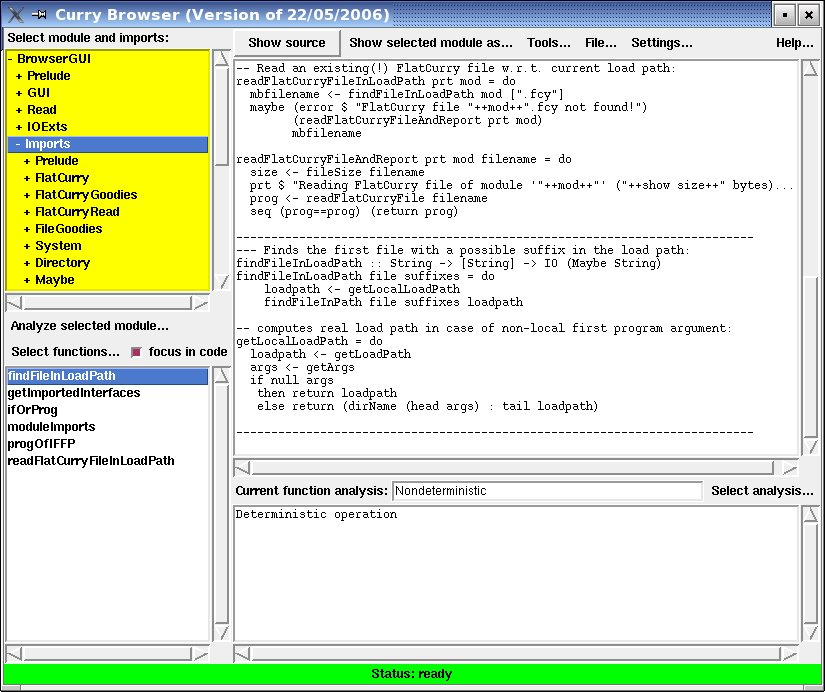
\includegraphics[scale=0.7]{currybrowser.jpg}
\end{center}
\caption{Snapshot of the main window of CurryBrowser\label{fig-currybrowser}}
\end{figure}
%
To get an impression of the use of \cb, Figure~\ref{fig-currybrowser}
shows a snapshot of its use on a particular application
(here: the implementation of \cb).
The upper list box in the left column shows the modules and their imports
in order to browse through the modules of an application.
Similarly to directory browsers, the list of imported modules of a module
can be opened or closed by clicking.
After selecting a module in the list of modules, its source code,
interface, or various other formats of the module can be shown
in the main (right) text area. For instance, one can show
pretty-printed versions of the intermediate flat programs (see below)
in order to see how local function definitions are translated by lambda lifting
\cite{Johnsson85}
or pattern matching is translated into case expressions \cite{Hanus97POPL,Wadler87}.
Since Curry is a language with parametric polymorphism and type inference,
programmers often omit the type signatures when defining functions.
Therefore, one can also view (and store) the selected module as source code where
missing type signatures are added.

Below the list box for selecting modules, there is a menu
(``Analyze selected module'') to analyze all functions
of the currently selected module at once. This is useful
to spot some functions of a module that could be problematic
in some application contexts, like functions that are impure (i.e., the result
depends on the evaluation time) or partially defined (i.e.,
not evaluable on all ground terms).
If such an analysis is selected,
the names of all functions are shown in the
lower list box of the left column (the ``function list'')
with prefixes indicating the properties of the individual functions.

The function list box can be also filled with functions
via the menu ``Select functions''. For instance, all functions
or only the exported functions defined in the currently selected
module can be shown there, or all functions from different modules
that are directly or indirectly called from
a currently selected function.
This list box is central to focus on a function in the
source code of some module or to analyze some function,
i.e., showing their properties. In order to focus on a function,
it is sufficient to check the ``focus on code'' button.
To analyze an individually selected function, one can
select an analysis from the list of available program analyses
(through the menu ``Select analysis'').
In this case, the analysis results are either shown
in the text box below the main text area
or visualized by separate tools, e.g., by a graph drawing tool for
visualizing call graphs.
Some analyses are local, i.e., they need only to consider the local definition
of this function (e.g., ``Calls directly,'' ``Overlapping rules,''
``Pattern completeness''),
where other analyses are global, i.e.,
they consider the definitions of all functions directly or indirectly called
by this function (e.g., ``Depends on,'' ``Solution complete,''
``Set-valued'').
%
Finally, there are a few additional tools integrated into \cb,
for instance, to visualize the import relation between all modules
as a dependency graph. These tools are available through the ``Tools'' menu.

More details about the use of \cb and all built-in analyses
are available through the ``Help'' menu of \cb.


\newpage

\section{CurryTest: A Tool for Testing Curry Programs}
\label{sec-currytest}

CurryTest\index{CurryTest}\index{testing programs}\index{program!testing}
is a simple tool in the PAKCS distribution to write
and run repeatable tests. CurryTest simplifies the task
of writing test cases for a module and executing them.
The tool is easy to use. Assume one has implemented a module \code{MyMod}
and wants to write some test cases to test its functionality,
making regression tests in future versions, etc.
For this purpose, there is a system library \code{Assertion}
(Section~\ref{Library:Assertion}) which
contains the necessary definitions for writing tests.
In particular, it exports an abstract polymorphic type \ccode{Assertion a}
together with the following operations:
\startprog
assertTrue      :: String -> Bool -> Assertion ()
assertEqual     :: String -> a -> a -> Assertion a
assertValues    :: String -> a -> [a] -> Assertion a
assertSolutions :: String -> (a->Success) -> [a] -> Assertion a
assertIO        :: String -> IO a -> a -> Assertion a
assertEqualIO   :: String -> IO a -> IO a -> Assertion a
\stopprog
The expression \ccode{assertTrue $s$ $b$}
is an assertion (named $s$) that the expression $b$ has the value \code{True}.
Similarly, the expression \ccode{assertEqual $s$ $e_1$ $e_2$}
asserts that the expressions $e_1$ and $e_2$
must be equal (i.e., \code{$e_1$==$e_2$} must hold),
the expression \ccode{assertValues $s$ $e$ $vs$} asserts
that $vs$ is the multiset of all values of $e$,
and the expression \ccode{assertSolutions $s$ $c$ $vs$} asserts
that the constraint abstraction $c$ has the multiset of solutions $vs$.
Furthermore, the expression \ccode{assertIO $s$ $a$ $v$}
asserts that the I/O action $a$ yields the value $v$ whenever it is
executed, and
the expression \ccode{assertEqualIO $s$ $a_1$ $a_2$}
asserts that the I/O actions $a_1$ and $a_2$ yields equal values.
The name $s$ provided as a first argument in each assertion
is used in the protocol produced by the test tool.

One can define a test program by importing the module
to be tested together with the module \code{Assertion} and defining
top-level functions of type \code{Assertion} in this module
(which must also be exported).
As an example, consider the following program
that can be used to test some list processing functions:
\startprog
\medskip
import List
import Assertion
\medskip
test1 = assertEqual     "++"     ([1,2]++[3,4]) [1,2,3,4]
\medskip
test2 = assertTrue      "all"    (all (<5) [1,2,3,4])
\medskip
test3 = assertSolutions "prefix" (\labs{}x -> let y free in  x\,++\,y =:= [1,2])
                                 [[],[1],[1,2]]
\medskip
\stopprog
For instance, \code{test1} asserts that the result of evaluating the
expression \code{([1,2]++[3,4])} is equal to \code{[1,2,3,4]}.

We can execute a test suite by the command\pindex{currytest}
\startprog
currytest testList
\stopprog
(\code{currytest} is a program stored in \code{$pakcshome$/bin}
where $pakcshome$ is the installation directory of PAKCS;
see Section~\ref{sec-general}).
In our example, \ccode{testList.curry} is the program containing the
definition of all assertions. This has the effect
that all exported top-level functions
of type \code{Assertion} are tested (i.e., the corresponding
assertions are checked) and the results
(\ccode{OK} or failure) are reported together with the name of each assertion.
%If failures occur, the complete test results are also
%written into a file named \ccode{testList.testlog}.''
For our example above, we obtain the following successful protocol:
\startprog
============================================================
Testing module "testList"...
OK: ++
OK: all
OK: prefix
All tests successfully passed.
============================================================
\stopprog
There is also a graphical interface that summarizes the results
more nicely.\footnote{Due to a bug in older versions of SICStus-Prolog,
it works only with SICStus-Prolog version 3.8.5 (or newer).}
In order to start this interface, one has to add the parameter
\ccode{--window} (or \ccode{-w}), e.g., executing a test suite by
\startprog
currytest --window testList
\stopprog
or
\startprog
currytest -w testList
\stopprog
A snapshot of the interface is shown in Figure~\ref{fig-currytest}.

\begin{figure}%[t]
\begin{center}
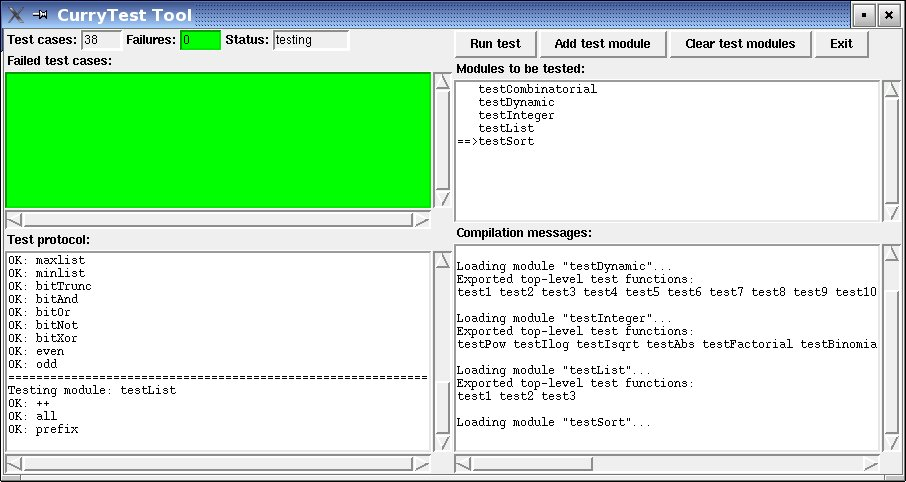
\includegraphics[scale=0.7]{currytest.jpg}
\end{center}
\caption{Snapshot of CurryTest's graphical interface\label{fig-currytest}}
\end{figure}


\newpage

\section{ERD2Curry: A Tool to Generate Programs from ER Specifications}
\label{sec-erd2curry}

ERD2Curry\index{ERD2Curry}\index{database programming}
is a tool to generate Curry code to access and manipulate data
persistently stored from
entity relationship diagrams.\index{entity relationship diagrams}
The idea of this tool is described in detail in
\cite{BrasselHanusMueller08PADL}.
Thus, we describe only the basic steps to use this tool
in the following.

If one creates an entity relationship diagram (ERD)
with the Umbrello UML Modeller, one has to store its
XML description in XMI format (as offered by Umbrello)
in a file, e.g., \ccode{myerd.xmi}.
This description can be compiled into a Curry program by the
command\pindex{erd2curry}
\startprog
erd2curry myerd.xmi
\stopprog
(\code{erd2curry} is a program stored in \code{$pakcshome$/bin}
where $pakcshome$ is the installation directory of PAKCS;
see Section~\ref{sec-general}).
If \code{MyData} is the name of the ERD, the Curry program file
\ccode{MyData.curry} is generated containing all the necessary
database access code as described in \cite{BrasselHanusMueller08PADL}.

If one does not want to use the Umbrello UML Modeller,
one can also create a textual description of the ERD
as a Curry term of type \code{ERD}
(w.r.t.\ the type definition given in module
\code{$pakcshome$/tools/erd2curry/ERD.curry})
and store it in some file, e.g., \ccode{myerd.term}.
This description can be compiled into a Curry program by the
command\pindex{erd2curry}
\startprog
erd2curry -t myerd.term
\stopprog
%
There is also the possibility to visualize an ERD term
as a graph with the graph visualization program \code{dotty}
(for this purpose, it might be necessary to adapt the definition
of the operation \code{dotCmd} in
\code{$pakcshome$/tools/erd2curry/ERD2Graph.curry}
according to your local environment).
This can be done by the command
\startprog
erd2curry -v myerd.term
\stopprog

\paragraph{Inclusion in the Curry application:}
To compile the generated database code, either
include the directory \code{$pakcshome$/tools/erd2curry}
into your Curry load path
(e.g., by setting  the environment variable
\ccode{CURRYPATH}\pindex{CURRYPATH}, see also Section~\ref{sec-modules})
or copy the file
\code{$pakcshome$/tools/erd2curry/ERDGeneric.curry}
into the directory of the generated database code.


\newpage

\section{UI: Declarative Programming of User Interfaces}
\label{sec-ui}

The PAKCS distribution contains a collection of libraries
to implement graphical user interfaces\index{user interface}
as well as web-based user interfaces
from declarative descriptions.
Exploiting these libraries, it is possible
to define the structure and functionality of a user interface
independent from the concrete technology.
Thus, a graphical user interface or a web-based user interface
can be generated from the same description by simply changing
the imported libraries.
This programming technique is described in detail in
\cite{HanusKluss09PADL}.

The libraries implementing these user interfaces are contained
in the directory
\startprog
$pakcshome$/tools/ui
\stopprog
Thus, in order to compile programs containing such user interface
specifications, one has to
include the directory \code{$pakcshome$/tools/ui}
into the Curry load path
(e.g., by setting  the environment variable
\ccode{CURRYPATH}\pindex{CURRYPATH}, see also Section~\ref{sec-modules}).
The directory
\startprog
$pakcshome$/tools/ui/examples
\stopprog
contains a few examples for such user interface specifications.


\newpage

\section{Preprocessing FlatCurry Files}
\label{sec-pakcspp}

The current parser allows to apply transformations on the intermediate
FlatCurry files after they are generated from the
corresponding Curry source file.
Currently, only the FlatCurry file corresponding to the main module
can be transformed.

A transformation can be specified as follows:
\begin{enumerate}
\item {\bf Options to \code{pakcs/bin/parsecurry}:}
\begin{description}
\item[\fbox{\code{--fpopt}}]\pindex{-fpopt}
Apply functional pattern optimization
(see \code{pakcs/tools/optimize/NonStrictOpt.curry} for details).

\item[\fbox{\code{--compact}}]\pindex{--compact}
Apply code compactification after parsing, i.e., transform the main
module and all its imported into one module and delete all
non-accessible functions.

\item[\fbox{\code{--compactexport}}]
Similar to \code{--compact} but delete all functions that are not accessible
from the exported functions of the main module.

\item[\fbox{\code{--compactmain:f}}]
Similar to \code{--compact} but delete all functions that are not accessible
from the function \ccode{f} of the main module.

\item[\fbox{\code{--fcypp cmd}}]\pindex{--fcypp}
Apply command \code{cmd} to the main module after parsing. This is useful to
integrate your own transformation into the compilation process.
Note that the command \ccode{cmd prog} should perform a transformation
on the FlatCurry file \code{prog.fcy}, i.e., it replaces the FlatCurry
file by a new one.
\end{description}

\item {\bf Setting the environment variable \code{FCYPP}:}\pindex{FCYPP}\\
For instance, setting \code{FCYPP} by
\startprog
export FCYPP="--fpopt"
\stopprog
will apply the functional pattern optimization if programs are compiled
and loaded in the PAKCS programming environment.


\item {\bf Putting options into the source code:}\pindex{PAKCS_OPTION_FCYPP}\\
If the source code contains a line with a comment of the form (the comment
must start at the beginning of the line)
\startprog
\{-\# PAKCS_OPTION_FCYPP <options> \#-\}
\stopprog
then the transformations specified by \code{<options>} are applied after
translating the source code into FlatCurry code. For instance,
the functional pattern optimization can be set by the comment
\startprog
\{-\# PAKCS_OPTION_FCYPP --fpopt \#-\}
\stopprog
in the source code. Note that this comment must be in a single line 
of the source program. If there are multiple lines containing such comments,
only the first one will be considered.
\end{enumerate}
\paragraph{Multiple options:}
Note that an arbitrary number of transformations can be specified
by the methods described above.
If several specifications for preprocessing FlatCurry files are used,
they are executed in the following order:
\begin{enumerate}
\item all transformations specified by the environemnt variable
\code{FCYPP} (from left to right)
\item all transformations specified as command line options of parsecurry
   (from left to right)
\item all transformations specified by a comment line in the source code
   (from left to right)
\end{enumerate}


\newpage

\section{Technical Problems}

Due to the fact that Curry is intended to implement
distributed systems (see Appendix~\ref{sec-ports}),
it might be possible that some technical problems
arise due to the use of sockets for implementing these
features. Therefore, this section gives some information
about the technical requirements of PAKCS and how to solve
problems due to these requirements.

There is one fixed port that is used by the implementation of PAKCS:
\begin{description}
\item[Port 8766:] This port is used by the
{\bf Curry Port Name Server} (CPNS) to implement symbolic names for
ports in Curry (see Appendix~\ref{sec-ports}).
If some other process uses this port on the machine,
the distribution facilities defined in the module \code{Ports}
(see Appendix~\ref{sec-ports}) cannot be used.
\end{description}
If these features do not work, you can try to find out
whether this port is in use by the shell command
\ccode{netstat -a | fgrep 8766} (or similar).

The CPNS is implemented as a demon listening on its port 8766
in order to serve requests about registering a new symbolic
name for a Curry port or asking the physical port number
of a Curry port. The demon will be automatically started for
the first time on a machine when a user compiles a program
using Curry ports. It can also be manually started and terminated by the
scripts \code{$pakcshome$/cpns/start} and
\code{$pakcshome$/cpns/stop}.
If the demon is already running, the command \code{$pakcshome$/cpns/start}
does nothing (so it can be always executed
before invoking a Curry program using ports).

If you detect any further technical problem,
please write to
\begin{center}
\code{mh@informatik.uni-kiel.de}
\end{center}

\newpage

\addcontentsline{toc}{section}{Bibliography}
\bibliography{manual}
\bibliographystyle{plain}

\newpage
\appendix

\section{Libraries of the PAKCS Distribution}
\label{sec:libraries}

{\setlength{\parindent}{0.0cm}

The PAKCS compiler system provides an extensive collection
of libraries for application programming.
The libraries for arithmetic constraints over real numbers,
finite domain constraints,
ports for concurrent and distributed programming, and
meta-programming by representing Curry programs in Curry
are described in the following subsection in more detail.
The complete set of libraries with all exported types and functions
are described in the further subsections.
For a more detailed online documentation of all libraries of PAKCS,
see \url{http://www.informatik.uni-kiel.de/~pakcs/lib/index.html}.

\subsection{Constraints, Ports, Meta-Programming}

\subsubsection{Arithmetic Constraints}

The primitive entities for the use of arithmetic constraints
are defined in the system module \code{CLPR}
(cf.\ Section~\ref{sec-modules}), i.e., in order to use them,
the program must contain the import declaration
\startprog
import CLPR
\stopprog
Floating point arithmetic is supported in PAKCS
via arithmetic constraints, i.e., the equational constraint
\ccode{2.3 +.~x =:= 5.5} is solved by binding \code{x} to \code{3.2}
(rather than suspending the evaluation of the addition,
as in corresponding constraints on integers like
\ccode{3+x=:=5}). All operations related to
floating point numbers are suffixed by \ccode{.}.
The following functions and constraints on floating point
numbers are supported in PAKCS:
\begin{description}
\item[\code{(+.)   :: Float -> Float -> Float}]~\\
Addition on floating point numbers.
\item[\code{(-.)   :: Float -> Float -> Float}]~\\
Subtraction on floating point numbers.
\item[\code{(*.)   :: Float -> Float -> Float}]~\\
Multiplication on floating point numbers.
\item[\code{(/.)   :: Float -> Float -> Float}]~\\
Division on floating point numbers.
\item[\code{(<.)   :: Float -> Float -> Success}]~\\
Comparing two floating point numbers with the ``less than'' relation.
\item[\code{(>.)   :: Float -> Float -> Success}]~\\
Comparing two floating point numbers with the ``greater than'' relation.
\item[\code{(<=.)  :: Float -> Float -> Success}]~\\
Comparing two floating point numbers with the ``less than or equal'' relation.
\item[\code{(>=.)  :: Float -> Float -> Success}]~\\
Comparing two floating point numbers with the ``greater than or equal''
relation.
\item[\code{i2f    :: Int -> Float}]~\\
Converting an integer number into a floating point number.
\end{description}
As an example, consider a constraint \code{mortgage}
which relates the principal \code{p},
the lifetime of the mortgage in months \code{t},
the monthly interest rate \code{ir},
the monthly repayment \code{r},
and the outstanding balance at the end of the lifetime \code{b}.
The financial calculations
can be defined by the following two rules in Curry (the second rule
describes the repeated accumulation of the interest):
\startprog
~
import CLPR
~
mortgage p t ir r b | t >. 0.0 \& t <=. 1.0  --lifetime not more than 1 month?
                    =  b =:= p *. (1.0 +. t *. ir) -. t*.r \vspace{1ex}
mortgage p t ir r b | t >. 1.0               --lifetime more than 1 month?
                    =  mortgage (p *. (1.0+.ir)-.r) (t-.1.0) ir r b
~
\stopprog
Then we can calculate the monthly payment for paying back
a loan of \$100,000 in 15 years with a monthly interest rate of 1\%
by solving the goal
\startprog
mortgage 100000.0 180.0 0.01 r 0.0
\stopprog
which yields the solution \code{r=1200.17}.

Note that only linear arithmetic equalities or inequalities
are solved by the constraint solver. Non-linear constraints
like \ccode{x *.~x =:= 4.0} are suspended until they become
linear.


\subsubsection{Finite Domain Constraints}

Finite domain constraints are constraints where all variables
can only take a finite number of possible values.
For simplicity, the domain of finite domain variables are
identified with a subset of the integers, i.e., the type
of a finite domain variable is \code{Int}. The arithmetic
operations related to finite domain variables are suffixed by \ccode{\#}.
The following functions and constraints for finite domain constraint solving
are currently supported in PAKCS:\footnote{Note that
this library is based on the corresponding library of SICStus-Prolog
but does not implement the complete functionality of the SICStus-Prolog library.
However, using the PAKCS interface for external functions (see
Appendix~\ref{sec-external-functions}), it is relatively
easy to provide the complete functionality.}

\begin{description}
\item[\code{domain :: [Int] -> Int -> Int -> Success}]~\\
The constraint \ccode{domain [$x_1,\ldots,x_n$] $l$ $u$}
is satisfied if the domain of all variables $x_i$ is the interval $[l,u]$.
\item[\code{(+\#)   :: Int -> Int -> Int}]~\\
Addition on finite domain values.
\item[\code{(-\#)   :: Int -> Int -> Int}]~\\
Subtraction on finite domain values.
\item[\code{(*\#)   :: Int -> Int -> Int}]~\\
Multiplication on finite domain values.
\item[\code{(=\#)   :: Int -> Int -> Success}]~\\
Equality of finite domain values.
\item[\code{(/=\#)  :: Int -> Int -> Success}]~\\
Disequality of finite domain values.
\item[\code{(<\#)   :: Int -> Int -> Success}]~\\
``less than'' relation on finite domain values.
\item[\code{(<=\#)  :: Int -> Int -> Success}]~\\
``less than or equal'' relation on finite domain values.
\item[\code{(>\#)   :: Int -> Int -> Success}]~\\
``greater than'' relation on finite domain values.
\item[\code{(>=\#)  :: Int -> Int -> Success}]~\\
``greater than or equal'' relation on finite domain values.
\item[\code{sum :: [Int] -> (Int -> Int -> Success) -> Int -> Success}]~\\
The constraint \ccode{sum [$x_1,\ldots,x_n$] $op$ $x$}
is satisfied if all $x_1+\cdots + x_n \mathrel{op} x$ is satisfied,
where $op$ is one of the above finite domain constraint relations
(e.g., \ccode{=\#}).
\item[\code{scalar_product :: [Int] -> [Int] -> (Int -> Int -> Success) -> Int -> Success}]~\\
The constraint \ccode{scalar_product [$c_1,\ldots,c_n$] [$x_1,\ldots,x_n$] $op$ $x$}
is satisfied if all $c_1 x_1+\cdots + c_n x_n \mathrel{op} x$ is satisfied,
where $op$ is one of the above finite domain constraint relations.
\item[\code{count :: Int -> [Int] -> (Int -> Int -> Success) -> Int -> Success}]~\\
The constraint \ccode{count $k$ [$x_1,\ldots,x_n$] $op$ $x$}
is satisfied if all $k \mathrel{op} x$ is satisfied,
where $n$ is the number of the $x_i$ that are equal to $k$ and
$op$ is one of the above finite domain constraint relations.
\item[\code{all_different :: [Int] -> Success}]~\\
The constraint \ccode{all_different [$x_1,\ldots,x_n$]}
is satisfied if all $x_i$ have pairwise different values.
\item[\code{labeling :: [LabelingOption] -> [Int] -> Success}]~\\
The constraint \ccode{labeling $os$ [$x_1,\ldots,x_n$]}
non-deterministically instantiates all $x_i$ to the values
of their domain according to the options $os$ (see the module documentation
for further details about these options).
\end{description}
These entities are defined in the system module \code{CLPFD}
(cf.\ Section~\ref{sec-modules}), i.e., in order to use it,
the program must contain the import declaration
\startprog
import CLPFD
\stopprog
As an example, consider the classical \ccode{send+more=money} problem
where each letter must be replaced by a different digit such that this
equation is valid and there are no leading zeros.
The usual way to solve finite domain constraint problems
is to specify the domain of the involved variables followed
by a specification of the constraints and the labeling
of the constraint variables in order to start the search for solutions.
Thus, the \ccode{send+more=money} problem can be solved as follows:
\startprog
~
import CLPFD
~
smm l =
        l =:= [s,e,n,d,m,o,r,y] \&
        domain l 0 9 \&
        s >\# 0 \&
        m >\# 0 \&
        all_different l  \&
                         1000 *\# s +\# 100 *\# e +\# 10 *\# n +\# d
        +\#               1000 *\# m +\# 100 *\# o +\# 10 *\# r +\# e
        =\# 10000 *\# m +\# 1000 *\# o +\# 100 *\# n +\# 10 *\# e +\# y \&
        labeling [FirstFail] l
        where s,e,n,d,m,o,r,y free
~
\stopprog
Then we can solve this problem by evaluating the goal
\ccode{smm [s,e,n,d,m,o,r,y]} which yields the unique solution
\code{\{s=9,e=5,n=6,d=7,m=1,o=0,r=8,y=2\}}.


\subsubsection{Ports: Distributed Programming in Curry}
\label{sec-ports}

To support the development of concurrent and distributed applications,
PAKCS supports internal and external ports\index{ports} as
described in \cite{Hanus99PPDP}.
Since \cite{Hanus99PPDP} contains a detailed description of this
concept together with various programming examples, we only summarize here
the functions and constraints supported for ports in PAKCS.

The basic datatypes, functions, and constraints for ports
are defined in the system module \code{Ports}
(cf.\ Section~\ref{sec-modules}), i.e., in order to use ports,
the program must contain the import declaration
\startprog
import Ports
\stopprog
This declaration includes the following entities in the program:
\begin{description}
\item[\code{Port a}\pindex{Port}]~\\
This is the datatype of a port to which one can send messages of type \code{a}.

\item[\code{openPort :: Port a -> [a] -> Success}]~\\
The constraint \ccode{openPort p s}\pindex{openPort}
establishes a new \emph{internal port}
\code{p} with an associated message stream \code{s}. \code{p} and \code{s} must be
unbound variables,
otherwise the constraint fails (and causes a runtime error).

\item[\code{send :: a -> Port a -> Success}]~\\
The constraint \ccode{send m p}\pindex{send}
is satisfied if \code{p} is constrained
to contain the message \code{m}, i.e., \code{m} will be sent to the port
\code{p} so that it appears in the corresponding stream.

\item[\code{doSend :: a -> Port a -> IO ()}]~\\
The I/O action \ccode{doSend m p}\pindex{doSend} solves the constraint
\ccode{send m p} and returns nothing.

\item[\code{openNamedPort :: String -> IO [a]}]~\\
The I/O action \ccode{openNamedPort n}\pindex{openNamedPort}
opens a new \emph{external port} with
symbolic name \code{n} and returns the associated stream of messages.

\item[\code{connectPort :: String -> IO (Port a)}]~\\
The I/O action \ccode{connectPort n}\pindex{connectPort}
returns a port with symbolic name
\code{n} (i.e., \code{n} must have the form ``\emph{portname@machine})
to which one can send messages by the \code{send} constraint.
Currently, no dynamic type checking is done for external ports,
i.e., sending messages of the wrong type to a port might lead to
a failure of the receiver.
\end{description}

\paragraph{Restrictions:}
Every expression, possibly containing logical variables, can be sent to
a port. However, as discussed in \cite{Hanus99PPDP},
port communication is strict, i.e., the expression is
evaluated to normal form before sending it by the
constraint \code{send}. Furthermore, if messages containing
logical variables are sent to \emph{external ports},
the behavior is as follows:
\begin{enumerate}
\item The sender waits until all logical variables in the message
have been bound by the receiver.
\item The binding of a logical variable received by a process
is sent back to the sender of this logical variable only if
it is bound to a \emph{ground} term, i.e., as long as the binding contains
logical variables, the sender is not informed about the binding
and, therefore, the sender waits.
\end{enumerate}

\paragraph{External ports on local machines:}
The implementation of external ports assumes that the
host machine running the application is connected to the Internet
(i.e., it uses the standard IP address of the host machine
for message sending). If this is not the case and the application
should be tested by using external ports only on the local host
without a connection to the Internet,
the environment variable \ccode{PAKCS_LOCALHOST}\pindex{PAKCS_LOCALHOST}
must be set to \ccode{yes}
\emph{before PAKCS system is started}.
In this case, the IP address \code{127.0.0.1} and the hostname
\ccode{localhost} are used for identifying the local machine.

\paragraph{Selection of Unix sockets for external ports:}
The implementation of ports uses sockets to communicate
messages sent to external ports.
Thus, if a Curry program uses the
I/O action \code{openNamedPort}\pindex{openNamedPort}
to establish an externally visible server,
PAKCS selects a Unix socket for the port communication.
Usually, a free socket is selected by the operating system.
If the socket number should be fixed in an application (e.g.,
because of the use of firewalls\index{firewall} that allow only
communication over particular sockets), then one
can set the environment variable \ccode{PAKCS_SOCKET}\pindex{PAKCS_SOCKET}
to a distinguished socket number before the PAKCS system is started.
This has the effect that PAKCS uses only this socket
number for communication (even for several external ports
used in the same application program).

\paragraph{Debugging:}
To debug distributed systems,
it is sometimes helpful to see all messages sent to external ports.
This is supported by the environment variable
\ccode{PAKCS_TRACEPORTS}.\pindex{PAKCS_TRACEPORTS}
If this variable is set to \ccode{yes}
\emph{before the PAKCS system is started}, then all
connections to external ports and all
messages sent and received on external ports are
printed on the standard error stream.


\subsubsection{AbstractCurry and FlatCurry: Meta-Programming in Curry}
\label{sec-flatcurry}

\index{AbstractCurry}
\index{FlatCurry}
To support meta-programming, i.e., the manipulation of Curry programs
in Curry, there are system modules \code{FlatCurry} and \code{AbstractCurry}
(stored in the directory \ccode{$pakcshome$/lib/meta})
which define datatypes for the representation
of Curry programs.
\code{AbstractCurry} is a more direct representation of a Curry program,
whereas \code{FlatCurry} is a simplified representation
where local function definitions are replaced by global definitions
(i.e., lambda lifting has been performed) and pattern matching
is translated into explicit case/or expressions.
Thus, \code{FlatCurry} can be used for more back-end oriented
program manipulations (or, for writing new back ends for Curry),
whereas \code{AbstractCurry} is intended for manipulations of
programs that are more oriented towards the source program.

Both modules contain predefined I/O actions to read programs
in the \code{AbstractCurry} (\code{readCurry}\pindex{readCurry})
or \code{FlatCurry}
(\code{readFlatCurry}\pindex{readFlatCurry}) format.
These actions parse the corresponding source program and return
a data term representing this program (according to the definitions
in the modules \code{AbstractCurry} and \code{FlatCurry}).

Since all datatypes are explained in detail in these modules,
we refer to the online documentation\footnote{%
\url{http://www.informatik.uni-kiel.de/~pakcs/lib/CDOC/FlatCurry.html} and
\url{http://www.informatik.uni-kiel.de/~pakcs/lib/CDOC/AbstractCurry.html}}
of these modules.

As an example, consider a program file \ccode{test.curry}
containing the following two lines:
\startprog
rev []     = []
rev (x:xs) = (rev xs) ++ [x]
\stopprog
Then the I/O action \code{(FlatCurry.readFlatCurry "test")} returns the
following term:
\startprog
 (Prog "test"
  ["Prelude"]
  []
  [Func ("test","rev") 1 Public
        (FuncType (TCons ("Prelude","[]") [(TVar 0)])
                  (TCons ("Prelude","[]") [(TVar 0)]))
        (Rule [0]
           (Case Flex (Var 0)
              [Branch (Pattern ("Prelude","[]") [])
                  (Comb ConsCall ("Prelude","[]") []),
               Branch (Pattern ("Prelude",":") [1,2])
                  (Comb FuncCall ("Prelude","++")
                        [Comb FuncCall ("test","rev") [Var 2],
                         Comb ConsCall ("Prelude",":")
                              [Var 1,Comb ConsCall ("Prelude","[]") []]
                        ])
              ]))]
  []
 )
\stopprog


%%%%%%%%%%%%%%%%%%%%%%%%%%%%%%%%%%%%%%%%%%%%%%%%%%%%%%%%%%%%%%%%%%%%%%%%%
% Definitions in order to LaTeX documents generated by "currydoc --tex"
%%%%%%%%%%%%%%%%%%%%%%%%%%%%%%%%%%%%%%%%%%%%%%%%%%%%%%%%%%%%%%%%%%%%%%%%%

\newcommand{\currymodule}[1]{\subsubsection{Library #1}\label{Library:#1}}
\newcommand{\currytypesstart}{\subsubsection*{Exported types:}}
\newcommand{\currytypesstop}{}
\newcommand{\currytypesynstart}[2]{{\tt type #2}\pindex{#1} \begin{quote}}
\newcommand{\currytypesynstop}{\end{quote}}
\newcommand{\currydatastart}[1]{{\tt data #1}\pindex{#1} \begin{quote}}
\newcommand{\currydatacons}{\end{quote}%
\begin{itemize}\item[] \hspace{-4ex}\emph{Exported constructors:}}
\newcommand{\currydatastop}{\end{itemize}}
\newcommand{\curryconsstart}[2]{\item {\tt #1~::~#2}\par}
\newcommand{\curryfuncstart}{\subsubsection*{Exported functions:}}
\newcommand{\curryfuncstop}{}
\newcommand{\curryfunctionstart}[2]{#2\pindex{#1}\begin{quote}}
\newcommand{\curryfunctionstop}{\end{quote}}
\newcommand{\curryfuncsig}[2]{{\tt #1~::~#2}}


\subsection{General Libraries}

\input{lib/AllSolutions}
\input{lib/Assertion}
\input{lib/Char}
\input{lib/CLPFD}
\input{lib/CLPR}
\input{lib/CLPB}
\input{lib/Combinatorial}
\input{lib/Constraint}
\input{lib/CSV}
\input{lib/Database}
\input{lib/DaVinci}
\input{lib/Directory}
\input{lib/Dynamic}
\input{lib/FileGoodies}
\input{lib/Float}
\input{lib/Global}
\input{lib/GlobalVariable}
\input{lib/GUI}
\input{lib/Integer}
\input{lib/IO}
\input{lib/IOExts}
\input{lib/JavaScript}
\input{lib/KeyDatabase}
\input{lib/KeyDatabaseSQLite}
\input{lib/KeyDB}
\input{lib/List}
\input{lib/Maybe}
\input{lib/NamedSocket}
\input{lib/Parser}
\input{lib/Ports}
\input{lib/Pretty}
\input{lib/Profile}
\input{lib/PropertyFile}
\input{lib/Read}
\input{lib/ReadNumeric}
\input{lib/ReadShowTerm}
\input{lib/SetFunctions}
\input{lib/Socket}
\input{lib/System}
\input{lib/Time}
%\input{lib/Tk}
\input{lib/Unsafe}


\subsection{Data Structures and Algorithms}

\input{lib/Array}
\input{lib/Dequeue}
\input{lib/FiniteMap}
\input{lib/GraphInductive}
\input{lib/Random}
\input{lib/RedBlackTree}
\input{lib/SetRBT}
\input{lib/Sort}
\input{lib/TableRBT}
\input{lib/Traversal}

\subsection{Libraries for Web Applications}

\input{lib/CategorizedHtmlList}
\input{lib/HTML}
\input{lib/HtmlParser}
\input{lib/Mail}
\input{lib/Markdown}
\input{lib/WUI}
\input{lib/URL}
\input{lib/XML}
\input{lib/XmlConv}

\subsection{Libraries for Meta-Programming}

\input{lib/AbstractCurry}
\input{lib/AbstractCurryPrinter}
\input{lib/CompactFlatCurry}
\input{lib/CurryStringClassifier}
\input{lib/FlatCurry}
\input{lib/FlatCurryGoodies}
\input{lib/FlatCurryRead}
\input{lib/FlatCurryShow}
\input{lib/FlatCurryTools}
\input{lib/FlatCurryXML}
\input{lib/FlexRigid}
\input{lib/PrettyAbstract}

} % end setlength parindent

\newpage

\input{markdown_syntax}

\newpage

\begin{figure}%[t]
\begin{center}
 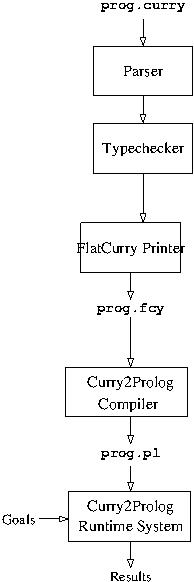
\includegraphics[scale=0.85]{pakcs_overview.jpg}
\end{center}\vspace{-5ex}
\caption{Overview of PAKCS\label{fig-pakcs}}
\end{figure}

\section{Overview of the PAKCS Distribution}

A schematic overview of the various components contained in
the distribution of PAKCS and the
translation process of programs inside PAKCS is shown in
Figure~\ref{fig-pakcs} on page~\pageref{fig-pakcs}.
In this figure, boxes denote different components of PAKCS
and names in boldface denote files containing
various intermediate representations during the translation
process (see Section~\ref{sec-auxfiles} below).
The PAKCS distribution contains a front end for reading (parsing and
type checking) Curry programs that can be also used by
other Curry implementations.
The back end (formerly known as ``Curry2Prolog''\index{Curry2Prolog})
compiles Curry programs into Prolog programs.
It also support constraint solvers for
arithmetic constraints over real numbers and finite domain constraints,
and further libraries for GUI programming, meta-programming etc.
Currently, it does not implement encapsulated search in full generality
(only a strict version of \code{findall} is supported),
and concurrent threads are not executed in a fair manner.


\newpage

\section{Auxiliary Files}
\label{sec-auxfiles}

During the translation and execution of a Curry program with PAKCS,
various intermediate representations of the source program are created
and stored in different files which are shortly explained in this section.
If you use the PAKCS, it is not necessary to know about
these auxiliary files because they are automatically generated
and updated. You should only remember the command for deleting
all auxiliary files (\ccode{cleancurry}, see Section~\ref{sec-general})
to clean up your directories.

The various components of PAKCS create
the following auxiliary files.
\begin{description}
\item[\code{prog.fcy}:] This file contains the Curry program
in the so-called ``FlatCurry'' representation where all functions are global
(i.e., lambda lifting has been performed) and pattern matching
is translated into explicit case/or expressions
(compare Appendix~\ref{sec-flatcurry}).
This representation might be useful for other back ends and
compilers for Curry and is the basis doing meta-programming in Curry.
This file is implicitly
generated when a program is read by PAKCS.
It can be also explicitly generated by the command\pindex{parsecurry}
\startprog
parsecurry --flat prog
\stopprog
The FlatCurry representation of a Curry program is usually
generated by the front-end after parsing, type checking and eliminating
local declarations.
If $dir$ is the directory where the Curry program is stored,
the corresponding FlatCurry program is stored in the directory
\ccode{$dir$/.curry}.

\item[\code{prog.fint}:] This file contains the interface
of the program in the so-called ``FlatCurry'' representation,
i.e., it is similar to \code{prog.fcy} but contains only exported
entities and the bodies of all functions omitted (i.e., ``external'').
This representation is useful for providing a fast access
to module interfaces.
This file is implicitly generated by the command\pindex{parsecurry}
\startprog
parsecurry --flat prog
\stopprog
and stored in the same directory as \code{prog.fcy}.

\item[\code{prog.pl}:] This file contains a Prolog program
as the result of translating the Curry program with PAKCS.
If $dir$ is the directory where the Curry program is stored,
the corresponding Prolog program is stored in the directory
\ccode{$dir$/.curry/.pakcs}.

\item[\code{prog.po}:] This file contains the Prolog program
\code{prog.pl} in an intermediate format for faster loading.
This file is stored in the same directory as \code{prog.pl}.

\item[\code{prog.state}:] This file contains the saved state
after compiling and saving a program with PAKCS
(see Section~\ref{sec-use-curry2prolog}).

\end{description}


\newpage


\section{Changing the Prelude or System Modules}

The standard prelude, which is automatically imported into each Curry program,
and all system modules containing datatypes and functions
useful for application programming
(cf.\ Appendix~\ref{sec:libraries})
are stored in the system module directory \ccode{$pakcshome$/lib}
(and its subdirectories).
If you change any of these modules,
you have to recompile the complete system by
executing \code{make} in the directory $pakcshome$.



\newpage

\section{External Functions}
\label{sec-external-functions}

\index{function!external}\index{external function}
Currently, PAKCS has no general interface to external functions.
Therefore, if a new external function should be added
to the system, this function must be declared as \code{external}
in the Curry source code
and then an implementation for this external function
must be inserted in the corresponding back end.
An external function is defined as follows in the Curry source code:
\begin{enumerate}
\item
Add a type declaration for the external function somewhere
in the body of the appropriate file (usually, the prelude
or some system module).
\item
For external functions it is not allowed to define any
rule since their semantics is determined by an external implementation.
Instead of the defining rules, you have to write
\startprog
f external
\stopprog
somewhere in the file containing the type declaration for 
the external function \code{f}.
\end{enumerate}
For instance, the addition on integers can be declared as
an external function as follows:
\startprog
(+) :: Int -> Int -> Int
(+) external
\stopprog
The further modifications to be done for an inclusion of
an external function has to be done in the back end.
A new external function is added to the back end of PAKCS
by informing the compiler about the existence of an external function
and adding an implementation of this function in the run-time
system. Therefore, the following items must be added
in the PAKCS compiler system:
\begin{enumerate}
\item
If the Curry module \code{Mod} contains external functions,
there must be a file named \code{Mod.prim_c2p} containing the
specification of these external functions. The contents of this file
is in XML format and has the following general structure:\footnote{%
\url{http://www.informatik.uni-kiel.de/~pakcs/primitives.dtd} contains a DTD
describing the exact structure of these files.}
\startprog
<primitives>
  \emph{specification of external function $f_1$}
  \ldots
  \emph{specification of external function $f_n$}
</primitives>
\stopprog
The specification of an external function $f$
with arity $n$ has the form
\startprog
<primitive name="$f$" arity="$n$">
  <library>lib</library>
  <entry>pred</entry>
</primitive>
\stopprog
where \code{lib} is the Prolog library (stored in the directory of the
Curry module or in the global directory
\code{$pakcshome$/curry2prolog/lib_src}) containing the code implementing this
function and \code{pred} is a predicate name in this library
implementing this function. Note that the function $f$ must be
declared in module \code{Mod}: either as an external function
or defined in Curry by equations. In the latter case,
the Curry definition is not translated but calls to this function
are redirected to the Prolog code specified above.

Furthermore, the list of specifications can also contain entries of the form
\startprog
<ignore name="$f$" arity="$n$" />
\stopprog
for functions $f$ with arity $n$ that are declared in module \code{Mod}
but should be ignored for code generation, e.g., since they are
never called w.r.t.\ to the current implementation of external functions.
For instance, this is useful when functions that can
be defined in Curry should be (usually more efficiently) are implemented
as external functions.

Note that the arguments are passed in their current (possibly unevaluated) form.
Thus, if the external function requires the arguments to be evaluated
in a particular form, this must be done before calling the external function.
For instance, the external function for adding two integers
requires that both arguments must be evaluated to non-variable head normal form
(which is identical to the ground constructor normal form). Therefore,
the function \ccode{+} is specified in the prelude by
\startprog
(+)   :: Int -> Int -> Int
x + y = (prim_Int_plus \$\# y) \$\# x
\medskip
prim_Int_plus :: Int -> Int -> Int
prim_Int_plus external
\stopprog
where \code{prim_Int_plus} is the actual external function implementing
the addition on integers. Consequently, the specification file
\code{Prelude.prim_c2p} has an entry of the form
\startprog
<primitive name="prim_Int_plus" arity="2">
  <library>prim_standard</library>
  <entry>prim_Int_plus</entry>
</primitive>
\stopprog
where the Prolog library \code{prim_standard.pl} contains the Prolog code
implementing this function.

\item
For most external functions, a \emph{standard interface} is
generated by the compiler so that an $n$-ary function can be
implemented by an $(n+1)$-ary predicate where the last argument must
be instantiated to the result of evaluating the function.  The
standard interface can be used if all arguments are ensured to be
fully evaluated (e.g., see definition of \code{(+)} above) and no
suspension control is necessary, i.e., it is ensured that the
external function call does not suspend for all arguments.
Otherwise, the raw interface (see below) must be used.  For
instance, the Prolog code implementing \code{prim_Int_plus}
contained in the Prolog library \code{prim_standard.pl} is as
follows (note that the arguments of \code{(+)} are passed in reverse
order to \code{prim_Int_plus} in order to ensure a left-to-right
evaluation of the original arguments by the calls to \code{(\$\#)}):
\startprog
prim_Int_plus(Y,X,R) :- R is X+Y.
\stopprog

\item
The \emph{standard interface for I/O actions}, i.e., external functions
with result type \code{IO~a}, assumes that the I/O action
is implemented as a predicate (with a possible side effect)
that instantiates the last argument to the returned value of type \ccode{a}.
For instance, the primitive predicate \code{prim_getChar}
implementing prelude I/O action \code{getChar}
can be implemented by the Prolog code
\startprog
prim_getChar(C) :- get_code(N), char_int(C,N).
\stopprog
where \code{char_int} is a predicate relating the internal
Curry representation of a character with its ASCII value.

\item
If some arguments passed to the external functions are not fully evaluated
or the external function might suspend, the implementation must follow
the structure of the PAKCS run-time system by using
the \emph{raw interface}. In this case, the name of the external entry
must be suffixed by \ccode{[raw]} in the \code{prim_c2p} file.
For instance, if we want to use the raw interface for the external function
\code{prim_Int_plus},
the specification file \code{Prelude.prim_c2p} must have an entry of the form
\startprog
<primitive name="prim_Int_plus" arity="2">
  <library>prim_standard</library>
  <entry>prim_Int_plus[raw]</entry>
</primitive>
\stopprog
In the raw interface, the actual implementation of an $n$-ary external function consists
of the definition of an $(n+3)$-ary predicate $pred$.
The first $n$ arguments are the corresponding actual arguments.
The $(n+1)$-th argument is a free variable which must be
instantiated to the result of the function call after
successful execution. The last two arguments
control the suspension behavior of the function
(see \cite{AntoyHanus00FROCOS} for more details):
The code for the predicate $pred$
should only be executed when the $(n+2)$-th argument
is not free, i.e., this predicate has always the
SICStus-Prolog block declaration
\startprog
?- block $pred$(?,\ldots,?,-,?).
\stopprog
In addition, typical external functions should suspend
until the actual arguments are instantiated. This can be ensured
by a call to \code{ensureNotFree} or \code{(\$\#)}
before calling the external function. Finally, the
last argument (which is a free variable at call time)
must be unified with the $(n+2)$-th argument
after the function call is successfully evaluated
(and does not suspend). Additionally, the actual (evaluated) arguments
must be dereferenced before they are accessed.
Thus, an implementation
of the external function for adding integers is as follows in the raw interface:
\startprog
?- block prim_Int_plus(?,?,?,-,?).
prim_Int_plus(RY,RX,Result,E0,E) :-
     deref(RX,X), deref(RY,Y), Result is X+Y, E0=E.
\stopprog
Here, \code{deref} is a predefined predicate for dereferencing the
actual argument into a constant (and \code{derefAll} for dereferencing
complex structures).
\end{enumerate}
%
The Prolog code implementing the external functions must be accessible to the run-time
system of PAKCS by putting it into the directory containing the corresponding
Curry module or into the system directory
\code{$pakcshome$/curry2prolog/lib_src}.
Then it will be automatically loaded into the run-time environment
of each compiled Curry program.

Note that arbitrary functions implemented in C or Java can be connected to
PAKCS by using the corresponding interfaces of underlying Prolog system.


\newpage
\addcontentsline{toc}{section}{Index}
\printindex


\end{document}

\clearpage
\documentclass[11pt,fleqn]{article}

\usepackage{latexsym}
\usepackage{makeidx}
\usepackage{url}
\usepackage{xspace}
\usepackage{graphicx}

\input{version}

%%% ------------------------------------------------------------------

\usepackage[colorlinks,linkcolor=blue]{hyperref}
\hypersetup{bookmarksopen=true}
\hypersetup{bookmarksopenlevel=0}
\hypersetup{pdftitle={PAKCS: The Portland Aachen Kiel Curry System}}
\hypersetup{pdfauthor={Michael Hanus}}
%\hypersetup{pdfstartview=Title}
\hypersetup{pdfstartview=FitH}
\usepackage{thumbpdf}

%%% ------------------------------------------------------------------

\setlength{\textwidth}{16.5cm}
\setlength{\textheight}{23cm}
\renewcommand{\baselinestretch}{1.1}
\setlength{\topmargin}{-1cm}
\setlength{\oddsidemargin}{0cm}
\setlength{\evensidemargin}{0cm}
\setlength{\marginparwidth}{0.0cm}
\setlength{\marginparsep}{0.0cm}

\newlength{\figurewidth}
\setlength{\figurewidth}{\textwidth}
\addtolength{\figurewidth}{-0.4cm}

% font for program texts
\renewcommand{\tt}{\usefont{OT1}{cmtt}{m}{n}\selectfont}
\newcommand{\codefont}{\tt}

% environment for typing program texts:
\makeatletter
\newenvironment{prog}{\par\vspace{0.7ex}
\setlength{\parindent}{1.0cm}
\setlength{\parskip}{-0.1ex}
\obeylines\@vobeyspaces\tt}{\vspace{0.7ex}\noindent
}
\makeatother
\newcommand{\startprog}{\begin{prog}}
\newcommand{\stopprog}{\end{prog}\noindent}

% program text in normal text
\newcommand{\code}[1]{\mbox{\codefont #1}}

% program text in normal text with apostrophs
\newcommand{\ccode}[1]{``\mbox{\codefont #1}''}

\newcommand{\pindex}[1]{\index{#1@{\tt #1}}}  % program elements in index

\newcommand{\labs}{\mbox{\tt\char92}}  % lambda abstraction in Curry
\newcommand{\todo}[1]{\fbox{\sc To do: #1}}
\newcommand{\cb}{CurryBrowser\xspace}

% allow underscores in programs:
\catcode`\_=\active
\let_=\sb
\catcode`\_=12

% produce an index:
\makeindex

\begin{document}
\sloppy

\begin{titlepage}
\pdfbookmark[1]{Title}{Title}
\begin{center}
\fbox{
\begin{minipage}[t]{\figurewidth}
\begin{center}\vspace{10ex}
{\Huge\bf PAKCS \pakcsversion}\\[4ex]
{\huge The Portland Aachen Kiel Curry System}\\[7ex]
{\huge User Manual}\\[4ex]
\pakcsversiondate\\[6ex]
\Large
Michael Hanus$^1$ [editor] \\[3ex]
{\large Additional Contributors:}\\[2ex]
Sergio Antoy$^2$ \\
Bernd Bra\ss{}el$^3$ \\
Martin Engelke$^4$ \\
Klaus H\"oppner$^5$ \\
Johannes Koj$^6$ \\
Philipp Niederau$^7$ \\
Ramin Sadre$^8$ \\
Frank Steiner$^9$ \\[4ex]
\normalsize
(1) University of Kiel, Germany, {\tt mh@informatik.uni-kiel.de} \\
(2) Portland State University, USA, {\tt antoy@cs.pdx.edu} \\
(3) University of Kiel, Germany, {\tt bbr@informatik.uni-kiel.de} \\
(4) University of Kiel, Germany, {\tt men@informatik.uni-kiel.de} \\
(5) University of Kiel, Germany, {\tt klh@informatik.uni-kiel.de} \\
(6) RWTH Aachen, Germany, {\tt johannes.koj@sdm.de} \\
(7) RWTH Aachen, Germany, {\tt philipp@navigium.de} \\
(8) RWTH Aachen, Germany, {\tt ramin@lvs.informatik.rwth-aachen.de} \\
(9) LMU Munich, Germany, {\tt fst@bio.informatik.uni-muenchen.de} \\[5ex]~
\end{center}
\end{minipage}}
\end{center}
\end{titlepage}

\pdfbookmark[1]{Contents}{Contents}
\tableofcontents

\newpage

\addcontentsline{toc}{section}{Preface}
\section*{Preface}

This document describes PAKCS (formerly called ``PACS''),
an implementation of the multi-paradigm language Curry,
jointly developed at the University of Kiel, the Technical University
of Aachen and Portland State University.
Curry is a universal programming language aiming at the amalgamation
of the most important declarative programming paradigms,
namely functional programming and logic programming.  
Curry combines in a seamless way features from functional programming
(nested expressions, lazy evaluation, higher-order functions),
logic programming (logical variables, partial data structures,
built-in search), and concurrent programming (concurrent evaluation
of constraints with synchronization on logical variables).
Moreover, the PAKCS implementation of Curry also supports
the high-level implementation of distributed applications,
graphical user interfaces, and web services
(as described in more detail in \cite{Hanus99PPDP,Hanus00PADL,Hanus01PADL}).

We assume familiarity with the ideas and features
of Curry as described in the Curry language definition \cite{Hanus12Curry}.
Therefore, this document only explains the use of the different
components of PAKCS
and the differences and restrictions of PAKCS
(see Section~\ref{sec-restrictions})
compared with the language Curry (Version 0.8.3).


\bigskip

\subsection*{Acknowledgements}

This work has been supported in part by the DAAD/NSF grant INT-9981317,
the NSF grants CCR-0110496 and CCR-0218224,
the Acci\'on Integrada hispano-alemana HA1997-0073,
and the DFG grants Ha 2457/1-2, Ha 2457/5-1, and Ha 2457/5-2.

Many thanks to the users of PAKCS for bug reports, bug fixes, and improvements,
in particular, to Marco Comini, Sebastian Fischer, Massimo Forni,
Carsten Heine, Stefan Junge, Frank Huch, Parissa Sadeghi.


\newpage

\section{Overview of PAKCS}

\subsection{General Use}
\label{sec-general}

This version of PAKCS has been tested on Sun Solaris, Linux, and Mac OS X
systems. In principle, it should be also executable on other
platforms on which a Prolog system like SICStus-Prolog or SWI-Prolog exists
(see the file \code{INSTALL.html} in the PAKCS directory
for a description of the necessary software to install PAKCS).

All executable files required to use the different components
of PAKCS are stored in the directory \code{$pakcshome$/bin}
(where $pakcshome$ is the installation directory of the complete
PAKCS installation). You should add this directory
to your path (e.g., by the \code{bash} command
\ccode{export PATH=$pakcshome$/bin:\$PATH}).

The source code of the Curry program
must be stored in a file with the suffix \ccode{.curry},
e.g., \code{prog.curry}. 
Literate programs must be stored in files with the extension \ccode{.lcurry}.
They are automatically converted into corresponding
\ccode{.curry} files by deleting all lines not starting 
with \ccode{>} and removing the prefix \ccode{> } of the
remaining lines.

Since the translation of Curry programs with PAKCS creates
some auxiliary files (see Section~\ref{sec-auxfiles} for details),
you need write permission
in the directory where you have stored your Curry programs.
The auxiliary files for all Curry programs in the current
directory can be deleted by the command\pindex{cleancurry}
\startprog
cleancurry
\stopprog
(this is a shell script stored in the \code{bin} directory of the
PAKCS installation, see above).
The command
\startprog
cleancurry -r
\stopprog
also deletes the auxiliary files in all subdirectories.



\subsection{Restrictions on Curry Programs}
\label{sec-restrictions}

There are a few minor restrictions on Curry programs
when they are processed with PAKCS:
\begin{itemize}
\item
\index{singleton variables}\index{variables!singleton}
\emph{Singleton pattern variables}, i.e., variables that occur only once
in a pattern of the rule, should be denoted as an anonymous variable \ccode{_},
otherwise the parser will print a warning since this is a
typical source of programming errors.
\item
PAKCS translates all \emph{local declarations} into global functions with
additional arguments (``lambda lifting'', see Appendix~D of the
Curry language report).
Thus, in the various run-time systems, the definition of
functions with local declarations look different from
their original definition (in order to see the result
of this transformation, you can use the \cb, see
Section~\ref{sec-currybrowser}).
\item \index{tabulator stops}
Tabulator stops instead of blank spaces in source files are
interpreted as stops at columns 9, 17, 25, 33, and so on.
\item Threads created by a concurrent conjunction are not executed
in a fair manner (usually, threads corresponding to leftmost constraints
are executed with higher priority).
\item
Encapsulated search\index{encapsulated search}: In order
to allow the integration of non-deterministic computations
in programs performing I/O at the top-level, PAKCS supports
the search operators \code{findall}\pindex{findall}
and \code{findfirst}\pindex{findfirst}.
In contrast to the general definition of encapsulated search
\cite{HanusSteiner98PLILP}, the current implementation suspends
the evaluation of \code{findall} and \code{findfirst}
until the argument does not contain unbound global variables.
Moreover, the evaluation of \code{findall} is strict,
i.e., it computes all solutions before returning the
complete list of solutions.
It is recommended to use the system module \code{AllSolutions}
for encapsulating search.
\item
There is currently no general connection to external constraint solvers.
However, the PAKCS compiler provides constraint
solvers for arithmetic and finite domain constraints
(see Appendix~\ref{sec:libraries}).
\end{itemize}

% Layout rule:
% (from Sergio's email of June 2, 1998)
%This is the general rule.  There are two kinds of syntactic
%constructs that rely on the offside rule.  One kind has a keyword
%indicating the end of the construct.  "let ... in" is the only
%representative of this kind.  Upon recognition of the keyword
%"in", all the constructs relying on the offide rule nested within
%the "let...in" are closed.  The other kind has no closing keyword.
%"where" and "choice" are the only constructs of this kind.
%Constructs of this kind can be closed only by indentation.  Any
%line, including a comment, indented less that the construct
%terminates it.  The indentation of "where", "choice" and "let" is
%the indentation of the first token following the keyword of the
%construct.
%



\subsection{Modules in PAKCS}
\label{sec-modules}

The current implementation of PAKCS supports only flat module names,
i.e., the notation \code{Dir.Mod.f} is not supported.\index{modules}
In order to allow the structuring of modules in different directories,
PAKCS searches for imported modules in various directories.
By default, imported modules are searched in the directory
of the main program and the system module directories
\ccode{$pakcshome$/lib} and \ccode{$pakcshome$/lib/meta}.
This search path can be extended
by setting the environment variable \code{CURRYPATH}\pindex{CURRYPATH}
(which can be also set in a PAKCS session by the command
\ccode{:set path}\pindex{path}\pindex{:set path},
see below)
to a list of directory names separated by colons (\ccode{:}).
In addition, a local standard search path
can be defined in the \ccode{.pakcsrc} file
(see Section~\ref{sec-customization}).
Thus, modules to be loaded are searched in the following
directories (in this order, i.e., the first occurrence of a module file
in this search path is imported):
\begin{enumerate}
\item Current working directory (\ccode{.}) or directory prefix
of the main module (e.g., directory \ccode{/home/joe/curryprogs}
if one loads the Curry program \ccode{/home/joe/curryprogs/main}).
\item The directories enumerated in the environment variable \code{CURRYPATH}.
\item The directories enumerated in the \ccode{.pakcsrc} variable
      \ccode{libraries}.
\item The directories \ccode{$pakcshome$/lib} and \ccode{$pakcshome$/lib/meta}.
\end{enumerate}
Note that the standard prelude (\code{$pakcshome$/lib/Prelude.curry})
will be always implicitly imported to all modules if a module
does not contain an explicit import declaration for the module
\code{Prelude}.


\newpage

\section{PAKCS: An Interactive Curry Development System}
\label{sec-curry2prolog}

PAKCS\index{PAKCS},
in the following just called ``PAKCS'',
is an interactive system to develop applications
written in Curry.
It is implemented in Prolog and compiles
Curry programs into Prolog programs. It contains various tools,
a source-level debugger,
solvers for arithmetic constraints over real numbers
and finite domain constraints, etc. The compilation process and the
execution of compiled programs is fairly efficient
if a good Prolog implementation like SICStus-Prolog is used.


\subsection{How to Use PAKCS}
\label{sec-use-curry2prolog}

To start PAKCS, execute the command
\ccode{pakcs}\pindex{pakcs}
(this is a shell script stored in
\code{$pakcshome$/bin} where $pakcshome$ is the installation directory
of PAKCS).
When the system is ready, the prelude (\code{$pakcshome$/lib/Prelude.curry})
is already loaded, i.e., all definitions in the prelude are accessible.
Now you can type in various commands.
The {\bf most important commands} are
(it is sufficient to type a unique prefix of a command if it is unique,
e.g., one can type \ccode{:r} instead of \ccode{:reload}):

\begin{description}
\item[\fbox{\code{:help}}]\pindex{:help}
Show a list of all available commands.

\item[\fbox{\code{:load $prog$}}]\pindex{:load}
Compile and load the program stored in \code{$prog$.curry}
together with all its imported modules.
If this file does not exist, the system looks for a FlatCurry
file \code{$prog$.fcy} and compiles from this intermediate representation.
If the file \code{$prog$.fcy} does not exists, too, the system looks
for a file \code{$prog$_flat.xml} containing a FlatCurry program in
XML representation (compare command \ccode{:xml}\pindex{:xml}),
translates this into a FlatCurry file \code{$prog$.fcy}
and compiles from this intermediate representation.

\item[\fbox{\code{:reload}}]\pindex{:reload}
Recompile all currently loaded modules.

\item[\fbox{\code{:add} $m$}]\pindex{:add}
Add module $m$ to the set of currently loaded modules
so that its exported entities are available in the top-level environment.

\item[\fbox{$expr$}] Evaluate the expression $expr$ to normal form
and show the computed results. Since the PAKCS
compiles Curry programs into Prolog programs,
non-deterministic computations are implemented by backtracking.
Therefore, computed results are shown one after the other.
After each computed result, you will be asked whether
you want to see the next alternative result or all alternative results.
The default answer value for this question can be defined
in the \ccode{.pakcsrc} file (see Section~\ref{sec-customization}).

\textbf{Free variables in initial expressions} must be declared as in Curry programs
(if the free variable mode\index{free variable mode} is not turned on,
see option \ccode{+free} below), i.e.,
either by a \ccode{let\ldots{}free in}
or by a \ccode{where\ldots{}free} declaration.
For instance, one can write
\startprog
let xs,ys free in xs++ys\,=:=\,[1,2]
\stopprog
or
\startprog
xs++ys\,=:=\,[1,2]  where xs,ys free
\stopprog
Without these declarations, an error is reported in order to
avoid the unintended introduction of free variables in initial expressions
by typos.

Note that lambda abstractions, \code{let}s and list comprehensions
in top-level expressions are not yet supported in initial expressions
typed in the top-level of PAKCS.

\item[\fbox{\code{let} $x$ \code{=} $expr$}]
Define the identifier $x$ as an abbreviation for the expression $expr$
which can be used in subsequent expressions. The identifier $x$
is visible until the next \code{load} or \code{reload} command.

\item[\fbox{\code{:quit}}]\pindex{:quit} Exit the system.
\end{description}
%
\bigskip
%
There are also a number of {\bf further commands} that are often
useful:
%
\begin{description}
\item[\fbox{\code{:type $expr$}}]\pindex{:type}
Show the type of the expression $expr$.

\item[\fbox{\code{:analyze}}]\pindex{:analyze}
Analyze the currently loaded program for some properties.
Currently, there are the following analysis options:
\begin{description}
\item[\fbox{\code{functions}}]
Check properties of all functions defined
in the currently loaded Curry program (i.e., without the functions defined
in the prelude and imported modules).
Currently, the following properties are checked:
\begin{enumerate}
\item Which functions are defined by overlapping left-hand sides?
\item Which functions are indeterministic, i.e., contains an
      indirect/implicit call to a \code{send} constraint on ports
      (see Appendix~\ref{sec-ports}, which includes
      an implicit committed choice)?
\end{enumerate}
\item[\fbox{\code{icalls}}]
Show all calls to imported functions in the currently loaded module.
This might be useful to see which import declarations are really necessary.
\end{description}

\item[\fbox{\code{:browse}}]\pindex{:browse}
Start the CurryBrowser to analyze the currently loaded
module together with all its imported modules
(see Section~\ref{sec-currybrowser} for more details).

\item[\fbox{\code{:edit}}]\pindex{:edit}
Load the source code of the current main module into a text editor.
If the environment variable \ccode{EDITOR} is set,
the value of this environment variable is used as the editor program,
otherwise a default editor (e.g., \ccode{vi}) is used.

\item[\fbox{\code{:edit $file$}}]\pindex{:edit}
Load file $file$ into a text editor which is defined
as in the command \ccode{:edit}.

\item[\fbox{\code{:interface}}]\pindex{:interface}
Show the interface of the currently loaded
module, i.e., show the names of all imported modules,
the fixity declarations of all exported operators,
the exported datatypes declarations and the types
of all exported functions.

\item[\fbox{\code{:interface $prog$}}]\pindex{:interface}
Similar to \ccode{:interface}
but shows the interface of the module \ccode{$prog$.curry}.
If this module does not exist, this command looks in the
system library directory of PAKCS for a module with this name,
e.g., the command \ccode{:interface FlatCurry} shows the interface
of the system module \code{FlatCurry} for meta-programming
(see Appendix~\ref{sec-flatcurry}).

\item[\fbox{\code{:modules}}]\pindex{:modules}
Show the list of all currently loaded modules.

\item[\fbox{\code{:programs}}]\pindex{:programs}
Show the list of all Curry programs that are available in the load path.

\item[\fbox{\code{:set $option$}}]\pindex{:set}
Set or turn on/off a specific option
of the PAKCS environment. Options are turned on by the prefix
\ccode{+} and off by the prefix \ccode{-}. Options that can only
be set (e.g., \code{printdepth}) must not contain a prefix.
The following options are currently supported:

\begin{description}
\item[\fbox{\code{+/-debug}}]\pindex{debug} Debug mode.
\index{debug mode}
In the debug mode, one can trace the evaluation of an expression,
setting spy points (break points) etc.\ (see the commands
for the debug mode described below).

\item[\fbox{\code{+/-free}}]\pindex{free} Free variable mode.\index{free variable mode}
If the free variable mode is off (default), then
free variables occurring in initial expressions entered in the
PAKCS environment must always be declared by a \ccode{let\ldots{}free in}
or \ccode{where\ldots{}free} declaration (as in Curry programs).
This avoids the introduction of free variables in initial expressions
by typos (which might lead to the exploration of infinite search spaces).
If the free variable mode is on, each undefined symbol
in an initial expression is considered as a free variable.

\item[\fbox{\code{+/-printfail}}]\pindex{printfail} Print failures.
If this option is set, failures occurring during evaluation
(i.e., non-reducible demanded subexpressions) are printed.
This is useful to see failed reductions due to partially
defined functions or failed unifications.
Inside encapsulated search (e.g., inside evaluations of
\code{findall} and \code{findfirst}), failures are not printed
(since they are a typical programming technique there).
Note that this option causes some overhead in execution time
and memory so that it could not be used in larger applications.

\item[\fbox{\code{+/-allfails}}]\pindex{allfails}
If this option is set, \emph{all} failures
(i.e., also failures on backtracking and failures
of enclosing functions that fail due to the failure of an argument
evaluation) are printed if the option \code{printfail} is set.
Otherwise, only the first failure (i.e., the first non-reducible
subexpression) is printed.

\item[\fbox{\code{+/-consfail}}]\pindex{consfail} Print constructor failures.
If this option is set, failures due to application of
functions with non-exhaustive pattern matching or failures
during unification (application of \ccode{=:=}) are shown.
Inside encapsulated search (e.g., inside evaluations of
\code{findall} and \code{findfirst}), failures are not printed
(since they are a typical programming technique there).
In contrast to the option \code{printfail},
this option creates only a small overhead in execution time
and memory use.

\item[\fbox{\code{+consfail all}}]\pindex{consfail}
Similarly to \ccode{+consfail}, but the complete trace
of all active (and just failed) function calls from the main function
to the failed function are shown.

\item[\fbox{\code{+consfail file:$f$}}]\pindex{consfail}
Similarly to \ccode{+consfail all}, but the complete fail trace
is stored in the file $f$. This option is useful in non-interactive
program executions like web scripts.

\item[\fbox{\code{+consfail int}}]\pindex{consfail}
Similarly to \ccode{+consfail all}, but after each failure occurrence,
an interactive mode for exploring the fail trace is started
(see help information in this interactive mode).
When the interactive mode is finished, the program execution
proceeds with a failure.

\item[\fbox{\code{+/-compact}}]\pindex{compact}
Reduce the size of target programs by using the
parser option \ccode{--compact}
(see Section~\ref{sec-pakcspp} for details about this option).

\item[\fbox{\code{+/-profile}}]\pindex{profile} Profile mode.
If the profile mode is on, then information about
the number of calls, failures, exits etc.\ are collected for
each function during the debug mode (see above) and shown
after the complete execution (additionaly, the result is stored
in the file \code{$prog$.profile} where $prog$ is the current main program).
The profile mode has no effect outside the debug mode.


\item[\fbox{\code{+/-suspend}}] Suspend mode (initially, it is off).
If the suspend mode is on, all suspended expressions
(if there are any) are shown (in their internal representation) at the end
of a computation.

\item[\fbox{\code{+/-time}}]\pindex{time} Time mode. If the time mode is on,
the cpu time and the elapsed time
of the computation is always printed together with the result
of an evaluation.

\item[\fbox{\code{+/-verbose}}] Verbose mode (initially, it is off).
If the verbose mode is on,
the initial expression of a computation (together with its type)
is printed before this expression is evaluated.

\item[\fbox{\code{+/-warn}}]\pindex{warn} Parser warnings. If the parser
warnings are turned on (default), the parser will print
warnings about variables that occur only once in a program rule
(see Section~\ref{sec-restrictions})
or locally declared names that shadow the definition of
globally declared names. If the parser warnings are switched off,
these warnings are not printed during the reading of a Curry program.

\item[\fbox{\code{path $path$}}]\pindex{path} Set the additional search path
for loading modules to $path$.
Note that this search path is only used for loading modules
inside this invocation of PAKCS, i.e., the environment variable
\ccode{CURRYPATH}\pindex{CURRYPATH} (see also Section~\ref{sec-modules})
is set to $path$ in this invocation of PAKCS.

\item[\fbox{\code{printdepth $n$}}]\pindex{printdepth}
Set the depth for printing terms to the value \code{n} (initially: 10).
In this case subterms with a depth greater than \code{n} are abbreviated
by dots when they are printed as a result of a computation
or during debugging. A value of \code{0} means infinite depth
so that the complete terms are printed.

\end{description}

\item[\fbox{\code{:set}}]\pindex{:set}
Show a help text on the \ccode{:set $option$}
command together with the current values of all options.

\item[\fbox{\code{:show}}]\pindex{:show}
Show the source text of the currently loaded Curry program.
If the environment variable \code{PAGER} is defined,
use its value to show the program, other use the command \ccode{more}.
If the source text is not available
(since the program has been directly compiled from a FlatCurry
or XML file), the loaded program is decompiled and
the decompiled Curry program text is shown.

\item[\fbox{\code{:show $m$}}]\pindex{:show}
Show the source text of module $m$ which must be accessible
via the current load path.

\item[\fbox{\code{:show $f$}}]\pindex{:show}
Show the source code of function $f$ (provided that the name $f$
is different from a module accessilbe via the current load path)
in a separate window.

\item[\fbox{\code{:cd $dir$}}]\pindex{:cd}
Change the current working directory to $dir$.

\item[\fbox{\code{:dir}}]\pindex{:dir} Show the names of all Curry programs
in the current working directory.

\item[\fbox{\code{:!$cmd$}}]\pindex{:"!} Shell escape: execute $cmd$ in a Unix shell.

\item[\fbox{\code{:save}}]\pindex{:save} Save the current state of the system
(together with the compiled program \code{prog.curry}) in the file
\code{prog.state}, i.e., you can later start the program again
by typing \ccode{prog.state} as a Unix command.

\item[\fbox{\code{:save $expr$}}]\pindex{:save} Similar as \ccode{:save}
but the expression $expr$ (typically: a call to the main
function) will be executed after restoring the state
and the execution of the restored state terminates when
the evaluation of the expression $expr$ terminates.

\item[\fbox{\code{:fork $expr$}}]\pindex{:fork}
The expression $expr$, which must be of type \ccode{IO ()},
is evaluated in an independent process which runs in
parallel to the current PAKCS process.
All output and error messages from this new process are suppressed.
This command is useful to test distributed Curry programs
(see Appendix~\ref{sec-ports}) where one can start
a new server process by this command. The new process
will be terminated when the evaluation of the expression $expr$
is finished.

\item[\fbox{\code{:coosy}}]\pindex{:coosy}
Start the Curry Object Observation System COOSy,
a tool to observe the execution of Curry programs.
This commands starts a graphical user interface to show
the observation results and adds to the load path the directory
containing the modules that must be imported in order to annotate
a program with observation points.
Details about the use of COOSy can be found in the
COOSy interface (under the ``Info'' button), and details
about the general idea of observation debugging and the implementation
of COOSy can be found in \cite{BrasselChitilHanusHuch04PADL}.

\item[\fbox{\code{:xml}}]\pindex{:xml}
Translate the currently loaded program module into an XML representation
according to the format described in
\url{http://www.informatik.uni-kiel.de/~curry/flat/}.
Actually, this yields an implementation-independent
representation of the corresponding FlatCurry program
(see Appendix~\ref{sec-flatcurry} for a description of FlatCurry).
If $prog$ is the name of the currently loaded program,
the XML representation will be written into the file \ccode{$prog$_flat.xml}.

\item[\fbox{\code{:peval}}]\pindex{:peval}
Translate the currently loaded program module into an equivalent
program where some subexpressions are partially evaluated
so that these subexpressions are (hopefully) more efficiently executed.
An expression $e$ to be partially evaluated
must be marked in the source program by \code{(PEVAL e)}
(where \code{PEVAL} is defined as the identity function in the prelude
so that it has no semantical meaning).

The partial evaluator
translates a source program \code{$prog$.curry} into the
partially evaluated program in intermediate representation
stored in \code{$prog$_pe.fcy}. The latter program is implicitly loaded
by the \code{peval} command so that the partially evaluated program
is directly available. The corresponding source program
can be shown by the \code{show} command (see above).

The current partial evaluator is an experimental prototype
(so it might not work on all programs) based on the ideas
described in \cite{AlbertAlpuenteHanusVidal99LPAR,AlbertHanusVidal00LPAR,%
AlbertHanusVidal01FLOPS,AlbertHanusVidal02JFLP}.

\end{description}
%
\bigskip
%
PAKCS can also execute programs in the {\bf debug mode}.
\index{debug mode}\pindex{debug}
The debug mode is switched on by setting the \code{debug} option
with the command \ccode{:set +debug}. In order to switch
back to normal evaluation of the program, one has to execute
the command \ccode{:set -debug}.

In the debug mode, PAKCS offers the following
{\bf additional options for the \ccode{:set} command:}
%
\begin{description}
\item[\fbox{\code{+/-single}}]\pindex{single}
Turn on/off single mode for debugging.
If the single mode is on, the evaluation of an expression
is stopped after each step and the user is asked how to proceed
(see the options there).

\item[\fbox{\code{+/-trace}}]\pindex{trace}
Turn on/off trace mode for debugging.
If the trace mode is on, all intermediate expressions occurring
during the evaluation of an expressions are shown.

\item[\fbox{\code{spy $f$}}]\pindex{spy}
Set a spy point (break point) on the
function $f$. In the single mode, you can ``leap'' from spy point
to spy point (see the options shown in the single mode).

\item[\fbox{\code{+/-spy}}]\pindex{spy} Turn on/off spy mode for debugging.
If the spy mode is on, the single mode is automatically activated
when a spy point is reached.
\end{description}


\subsection{Command Line Editing}

In order to have support for line editing or history functionality
in the command line of PAKCS (as often supported by the \code{readline}
library), you should have the Unix command \code{rlwrap} installed
on your local machine.
If \code{rlwrap} is installed, it is used by PAKCS if called on a terminal.
If it should not be used (e.g., because it is executed
in an editor with \code{readline} functionality), one can
call PAKCS with the parameter \ccode{--noreadline}.


\subsection{Customization}
\label{sec-customization}

In order to customize the behavior of PAKCS to your own preferences,
there is a configuration file which is read by PAKCS when it is invoked.
When you start PAKCS for the first time, a standard version of
this configuration file is copied with the name
\ccode{.pakcsrc}\pindex{pakcsrc}\pindex{.pakcsrc}
into your home directory. The file contains definitions
of various settings, e.g., about showing warnings, progress messages etc.
After you have started PAKCS for the first time, look into this file
and adapt it to your own preferences.


\subsection{Emacs Interface}

Emacs is a powerful programmable editor suitable for program development.
It is freely available for many platforms
(see \url{http://www.emacs.org} or \url{http://www.xemacs.org}).
The distribution of PAKCS contains also a special
\emph{Curry mode}\index{Curry mode}\index{Emacs}
that supports the development of Curry programs in
the (X)Emacs environment.
This mode includes support for syntax highlighting,
finding declarations in the current buffer, and
loading Curry programs into the PAKCS compiler system
in an Emacs shell.

The Curry mode has been adapted from a similar mode for Haskell programs.
Its installation is described in the file \code{README}
in directory \ccode{$pakcshome$/tools/emacs} which also contains
the sources of the Curry mode and a short description about
the use of this mode.


\newpage

\section{Extensions}
\label{sec-extensions}

PAKCS supports some extensions in Curry programs that are not (yet)
part of the definition of Curry. These extensions are described below.

\subsection{Recursive Variable Bindings}

Local variable declarations (introduced by \code{let}\pindex{let}
or \code{where}\pindex{where}) can be (mutually) recursive in PAKCS.
For instance, the declaration
\startprog
ones5 = let ones = 1 : ones
         in take 5 ones
\stopprog
introduces the local variable \code{ones} which is bound
to a \emph{cyclic structure}\index{cyclic structure}
representing an infinite list of \code{1}'s.
Similarly, the definition
\startprog
onetwo n = take n one2
 where
   one2 = 1 : two1
   two1 = 2 : one2
\stopprog
introduces a local variables \code{one2} that represents
an infinite list of alternating \code{1}'s and \code{2}'s
so that the expression \code{(onetwo 6)} evaluates to \code{[1,2,1,2,1,2]}.


\subsection{Functional Patterns}

Functional patterns \cite{AntoyHanus05LOPSTR} are a useful extension
to code operations in a more readable way. Furthermore,
defining operations with functional patterns avoids problems
caused by strict equality (\ccode{=:=}) and leads to programs
that are potentially more efficient.

Consider the definition of an operation to compute the last element
of a list \code{xs} based on the prelude operation \ccode{++}
for list concatenation:
\startprog
last xs | _++[y] =:= xs  = y   where y free
\stopprog
Since the equality constraint \ccode{=:=} evaluates both sides
to a constructor term, all elements of the list \code{xs} are
fully evaluated in order to satisfy the constraint.

Functional patterns can help to improve this computational behavior.
A \emph{functional pattern}\index{functional pattern}\index{pattern!functional}
is a function call at a pattern position. With functional patterns,
we can define the operation \code{last} as follows:
\startprog
last (_++[y]) = y
\stopprog
This definition is not only more compact but also avoids the complete
evaluation of the list elements: since a functional pattern is considered
as an abbreviation for the set of constructor terms obtained by all
evaluations of the functional pattern to normal form (see
\cite{AntoyHanus05LOPSTR} for an exact definition), the previous
definition is conceptually equivalent to the set of rules
\startprog
last [y] = y
last [_,y] = y
last [_,_,y] = y
\ldots
\stopprog
which shows that the evaluation of the list elements is not demanded
by the functional pattern.

In general, a pattern of the form \code{($f$ $t_1$\ldots$t_n$)} ($n>0$)
is interpreted as a functional pattern if $f$ is not a visible constructor
but a defined function that is visible in the scope of the pattern.

\paragraph{Optimization of programs containing functional patterns.}
Since functions patterns can evaluate to non-linear constructor terms,
they are dynamically checked for multiple occurrences of
variables which are, if present, replaced by equality constraints
so that the constructor term is always linear
(see \cite{AntoyHanus05LOPSTR} for details).
Since these dynamic checks are costly and not necessary for
functional patterns that are guaranteed to evaluate to linear terms,
there is an optimizer for functional patterns that checks
for occurrences of functional patterns that evaluate always to
linear constructor terms and replace such occurrences
with a more efficient implementation.
This optimizer can be enabled by the following possibilities:
\begin{itemize}
\item
Set the environment variable \code{FCYPP} to \ccode{--fpopt}
before starting PAKCS, e.g., by the shell command
\startprog
export FCYPP="--fpopt"
\stopprog
Then the functional pattern optimization is applied if programs are compiled
and loaded in PAKCS.
\item
Put an option into the source code:
If the source code of a program
contains a line with a comment of the form (the comment
must start at the beginning of the line)
\startprog
\{-\# PAKCS_OPTION_FCYPP --fpopt \#-\}
\stopprog
then the functional pattern optimization is applied
if this program is compiled and loaded in PAKCS.
\end{itemize}
The optimizer also report errors in case of wrong uses of functional patterns
(i.e., in case of a function $f$ defined with functional patterns that
recursively depend on $f$).


\subsection {Records}
\label{records}

A record is a data structure for bundling several data of various types.
It consists of typed data fields where each field is associated with
a unique label. These labels can be used to construct, select or update
fields in a record.


Unlike labeled data fields in Haskell, records are 
not syntactic sugar but a real extension of the
language\footnote{The current version allows to transform records
  into abstract data types. Future extensions may not have
  this facility.}.
The basic concept is described in \cite{Leijen05} but the current
version does not yet provide all features mentioned there. 
The restrictions are explained in Section~\ref{sec-restrinrecs}.
 
\subsubsection{Record Type Declaration}
\label{sec-recordtypedecl}

It is necessary to declare a record type before a record
can be constructed or used. The declaration has the following form:
\startprog
type $R$ $\alpha_1$ \ldots $\alpha_n$ = \{ $l_1$ :: $\tau_1$, \ldots, $l_m$ :: $\tau_m$ \}
\stopprog
It introduces a new $n$-ary record type $R$ which represents a
record consisting of $m$ fields. Each field has a unique label $l_i$ 
representing a value of the type $\tau_i$. Labels
are identifiers which refer to the corresponding
fields. The following examples define some record types:
\startprog
type Person = \{name :: String, age :: Int\}
type Address = \{person :: Person, street :: String, city :: String\}
type Branch a b = \{left :: a, right :: b\}
\stopprog
It is possible to summarize different labels which have the same
type. For instance, the record \code{Address} can also be declared as follows:
\startprog
type Address = \{person :: Person, street,city :: String\}
\stopprog
The fields can occur in an arbitrary order. The example above
can also be written as
\startprog
type Address = \{street,city :: String, person :: Person\}
\stopprog
The record type can be used in every type expression to represent
the corresponding record, e.g.
\startprog
data BiTree = Node (Branch BiTree BiTree) | Leaf Int
\stopprog
\startprog
getName :: Person -> String
getName \ldots
\stopprog


Labels can only be used in the context of
records. They do not share the name space with 
functions/constructors/variables or type constructors/type variables. 
For instance it is possible to use 
the same identifier for a label and a function at the same time. Label
identifiers cannot be shadowed by other identifiers.


Like in type synonym declarations, recursive or mutually 
dependent record declarations are not allowed. Records can only
be declared at the top level. Further restrictions are described in
section \ref{sec-restrinrecs}.


\subsubsection{Record Construction}
\label{sec-recordconstr}

The record construction generates a record with initial values for
each data field. It has the following form:
\startprog
\{ $l_1$ := $v_1$, \ldots, $l_m$ := $v_m$ \}
\stopprog
It generates a record where each label $l_i$ refers to the
value $v_i$. The type of the record results from the record type
declaration where the labels $l_i$ are defined.
A mix of labels from different
record types is not allowed. All labels must be specified with 
exactly one assignment. Examples for record constructions are
\startprog
\{name := "Johnson", age := 30\}     -- generates a record of type 'Person'
\{left := True, right := 20\}        -- generates a record of type 'Branch'
\stopprog
Assignments to labels can occur in an arbitrary order. For instance a
record of type \code{Person} can also be generated as follows:
\startprog
\{age := 30, name := "Johnson"\}     -- generates a record of type 'Person'
\stopprog
Unlike labeled fields in record type declarations, 
record constructions can be used in expressions without any restrictions
(as well as all kinds of record expressions). For instance the following
expression is valid:
\startprog
\{person := \{name := "Smith", age := 20\},   -- generates a record of
 street := "Main Street",                  -- type 'Address'
 city   := "Springfield"\}
\stopprog


\subsubsection{Field Selection}
\label{sec-fieldsel}

The field selection is used to extract data from records. 
It has the following form:
\startprog
$r$ :> $l$
\stopprog
It returns the value to which the label $l$ refers to from the
record expression $r$. The label must occur in the declaration of
the record type of $r$.
An example for a field selection is:
\startprog
pers :> name
\stopprog
This returns the value of the label \code{name} from the record \code{pers}
(which has the type \code{Person}).
Sequential application of field selections are also possible:
\startprog
(addr :> person) :> age
\stopprog
The value of the label \code{age} is extracted from a record which itself
is the value of the label \code{person} in the record \code{addr}
(which has the type \code{Address}). When a field selection is used in
expressions, it has to be parenthesized.


\subsubsection{Field Update}
\label{sec-fieldupd}

Records can be updated by reassigning a new value to a label:
\startprog
\{$l_1$ := $v_1$, \ldots, $l_k$ := $v_k$ | $r$\}
\stopprog
The label $l_i$ is associated with the new value $v_i$ which
replaces the current value in the record $r$.
The labels must occur in the declaration 
of the record type of $r$. In contrast to record constructions,
it is not necessary to specify all labels of a record. 
Assignments can occur in an arbitrary order. It is not allowed to 
specify more than one assignment for a label in a record update.
Examples for record updates are:
\startprog
\{name := "Scott", age := 25 | pers\}
\{person := \{name := "Scott", age := 25 | pers\} | addr\}
\stopprog
In these examples \code{pers} is a record of type \code{Person} and \code{addr}
is a record of type \code{Address}. 


\subsubsection{Records in Pattern Matching}
\label{sec-recsinpm}

It is possible to apply pattern matching to records (e.g., in functions,
let expressions or case branches). Two kinds of record patterns
are available:
\startprog
\{$l_1$ = $p_1$, \ldots, $l_n$ = $p_n$\}
\{$l_1$ = $p_1$, \ldots, $l_k$ = $p_k$ | _\}
\stopprog
In both cases each label $l_i$ is specified with a pattern $p_i$. 
All labels must occur only once in the record pattern.
The first case is used to match the whole record. Thus, all labels
of the record must occur in the pattern. 
The second case is used to match only a part of
the record. Here it is not necessary to specify all labels.
This case is represented by a vertical bar followed by the underscore
(anonymous variable). It is
not allowed to use a pattern term instead of the underscore.


When trying to match a record against a record pattern, the 
patterns of the specified labels are matched against 
the corresponding values in the record expression. On success, all pattern
variables occurring in the patterns are replaced by their actual expression.
If none of the patterns matches, the computation fails.


Here are some examples of pattern matching with records:
\startprog
isSmith30 :: Person -> Bool
isSmith30 \{name = "Smith", age = 30\} = True
\stopprog
\startprog
startsWith :: Char -> Person -> Bool
startsWith c \{name = (d:_) | _\} = c == d
\stopprog
\startprog
getPerson :: Address -> Person
getPerson \{person = p | _\} = p
\stopprog
As shown in the last example, a field selection can also be obtained
by pattern matching.


\subsubsection{Export of Records}
\label{sec-exprecs}

Exporting record types and labels is very similar to exporting
data types and constructors. There are three ways 
to specify an export:
\begin{itemize}
\item \code{module $M$ (\ldots, $R$, \ldots) where} \\
  exports the record $R$ without any of its labels.
\item \code{module $M$ (\ldots, $R$(..), \ldots) where} \\
  exports the record $R$ together with all its labels.
\item \code{module $M$ (\ldots, $R$($l_1$,\ldots,$l_k$), \ldots) where} \\
  exports the record $R$ together with the labels $l_1$, \ldots, $l_k$.
\end{itemize}
%
Note that imported labels cannot be overwritten in record declarations
of the importing module. It is also not possible to import equal labels
from different modules.


\subsubsection{Restrictions in the Usage of Records}
\label{sec-restrinrecs}

In contrast to the basic concept in \cite{Leijen05}, PAKCS/Curry provides a
simpler version of records. Some of the features described there are
currently not supported or even restricted.

\begin{itemize}
\item Labels must be unique within the whole scope of the program.
  In particular, it is not allowed to define the same label within
  different records, not even when they are imported from other
  modules. However, it is possible to use equal identifiers for other
  entities without restrictions, since labels have an independent 
  name space.
\item The record type representation with labeled fields can only be
  used as the right-hand-side of a record type declaration. It is
  not allowed to use it in any other type annotation.
\item Records are not extensible or reducible. The structure of a
  record is specified in its record declaration and cannot be
  modified at the runtime of the program.
\item Empty records are not allowed.
\item It is not allowed  to use a pattern term
  at the right side of the vertical bar in a record pattern
  except for the underscore (anonymous pattern variable).
\item Labels cannot be sequentially associated with multiple values
  (record fields do not behave like stacks).
\end{itemize}


\newpage

%%%%%%%%%%%%%%%%%%%%%%%%%%%%%%%%%%%%%%%%%%%%%%%%%%%%%%%%%%%%%%%%%%%%%%%%%
% Definitions in order to LaTeX documents generated by "currydoc -tex"
%%%%%%%%%%%%%%%%%%%%%%%%%%%%%%%%%%%%%%%%%%%%%%%%%%%%%%%%%%%%%%%%%%%%%%%%%

\newcommand{\currymodule}[1]{\subsection*{Module #1}}
\newcommand{\currytypesstart}{\subsubsection*{Exported types:}}
\newcommand{\currytypesstop}{}
\newcommand{\currytypesynstart}[2]{{\tt type #2}\pindex{#1} \begin{quote}}
\newcommand{\currytypesynstop}{\end{quote}}
\newcommand{\currydatastart}[1]{{\tt data #1}\pindex{#1} \begin{quote}}
\newcommand{\currydatacons}{\end{quote}%
\begin{itemize}\item[] \hspace{-4ex}\emph{Exported constructors:}}
\newcommand{\currydatastop}{\end{itemize}}
\newcommand{\curryconsstart}[2]{\item {\tt #1~::~#2}\par}
\newcommand{\curryfuncstart}{\subsubsection*{Exported functions:}}
\newcommand{\curryfuncstop}{}
\newcommand{\curryfunctionstart}[2]{#2\pindex{#1}\begin{quote}}
\newcommand{\curryfunctionstop}{\end{quote}}
\newcommand{\curryfuncsig}[2]{{\tt #1~::~#2}}

% for downward compatibility:
\newcommand{\currytype}[3]{{\tt type #2}\pindex{#1} \begin{quote} #3 \end{quote}}
\newcommand{\currydata}[3]{{\tt data #1}\pindex{#1} \begin{quote}#2\end{quote}%
\begin{itemize}\item[] \hspace{-4ex}\emph{Exported constructors:} #3\end{itemize}}
\newcommand{\curryfunction}[3]{#2\pindex{#1}  \begin{quote}#3\end{quote}}
\newcommand{\currycons}[3]{\item {\tt #1~::~#2}\par #3}



\newpage

\section{\cb: A Tool for Analyzing and Browsing Curry Programs}
\label{sec-currybrowser}

\cb is a tool to browse through the modules and functions
of a Curry application, show them in various formats,
and analyze their properties.\footnote{Although \cb is
implemented in Curry, some functionalities of it require an
installed graph visualization tool (dot \url{http://www.graphviz.org/}),
otherwise they have no effect.}
Moreover, it is constructed in a way so that
new analyzers can be easily connected to \cb.
A detailed description of the ideas behind this tool can be
found in \cite{Hanus05WCFLP,Hanus06WLPE}.

\cb is part of the PAKCS distribution and can be
started in two ways:
\begin{itemize}
\item
In the command shell via the command: \code{$pakcshome$/bin/currybrowser mod}
\item
In the PAKCS environment after loading the module
\code{mod} and typing the command \ccode{:browse}.
\end{itemize}
Here, \ccode{mod} is the name of the main module of a Curry application.
After the start, \cb loads the interfaces of the main
module and all imported modules before a GUI is created
for interactive browsing.

\begin{figure}[t]
\begin{center}
 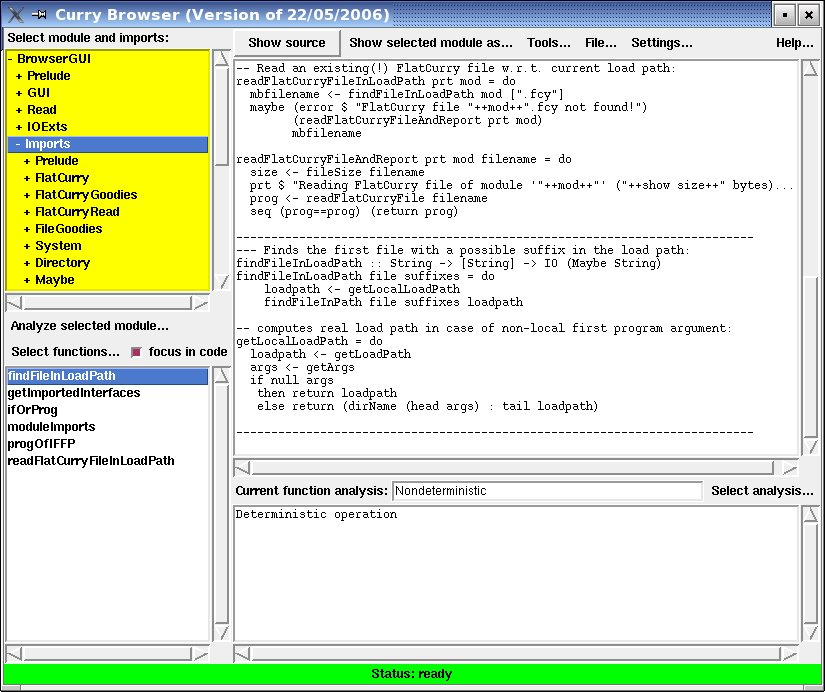
\includegraphics[scale=0.7]{currybrowser.jpg}
\end{center}
\caption{Snapshot of the main window of CurryBrowser\label{fig-currybrowser}}
\end{figure}
%
To get an impression of the use of \cb, Figure~\ref{fig-currybrowser}
shows a snapshot of its use on a particular application
(here: the implementation of \cb).
The upper list box in the left column shows the modules and their imports
in order to browse through the modules of an application.
Similarly to directory browsers, the list of imported modules of a module
can be opened or closed by clicking.
After selecting a module in the list of modules, its source code,
interface, or various other formats of the module can be shown
in the main (right) text area. For instance, one can show
pretty-printed versions of the intermediate flat programs (see below)
in order to see how local function definitions are translated by lambda lifting
\cite{Johnsson85}
or pattern matching is translated into case expressions \cite{Hanus97POPL,Wadler87}.
Since Curry is a language with parametric polymorphism and type inference,
programmers often omit the type signatures when defining functions.
Therefore, one can also view (and store) the selected module as source code where
missing type signatures are added.

Below the list box for selecting modules, there is a menu
(``Analyze selected module'') to analyze all functions
of the currently selected module at once. This is useful
to spot some functions of a module that could be problematic
in some application contexts, like functions that are impure (i.e., the result
depends on the evaluation time) or partially defined (i.e.,
not evaluable on all ground terms).
If such an analysis is selected,
the names of all functions are shown in the
lower list box of the left column (the ``function list'')
with prefixes indicating the properties of the individual functions.

The function list box can be also filled with functions
via the menu ``Select functions''. For instance, all functions
or only the exported functions defined in the currently selected
module can be shown there, or all functions from different modules
that are directly or indirectly called from
a currently selected function.
This list box is central to focus on a function in the
source code of some module or to analyze some function,
i.e., showing their properties. In order to focus on a function,
it is sufficient to check the ``focus on code'' button.
To analyze an individually selected function, one can
select an analysis from the list of available program analyses
(through the menu ``Select analysis'').
In this case, the analysis results are either shown
in the text box below the main text area
or visualized by separate tools, e.g., by a graph drawing tool for
visualizing call graphs.
Some analyses are local, i.e., they need only to consider the local definition
of this function (e.g., ``Calls directly,'' ``Overlapping rules,''
``Pattern completeness''),
where other analyses are global, i.e.,
they consider the definitions of all functions directly or indirectly called
by this function (e.g., ``Depends on,'' ``Solution complete,''
``Set-valued'').
%
Finally, there are a few additional tools integrated into \cb,
for instance, to visualize the import relation between all modules
as a dependency graph. These tools are available through the ``Tools'' menu.

More details about the use of \cb and all built-in analyses
are available through the ``Help'' menu of \cb.


\newpage

\section{CurryTest: A Tool for Testing Curry Programs}
\label{sec-currytest}

CurryTest\index{CurryTest}\index{testing programs}\index{program!testing}
is a simple tool in the PAKCS distribution to write
and run repeatable tests. CurryTest simplifies the task
of writing test cases for a module and executing them.
The tool is easy to use. Assume one has implemented a module \code{MyMod}
and wants to write some test cases to test its functionality,
making regression tests in future versions, etc.
For this purpose, there is a system library \code{Assertion}
(Section~\ref{Library:Assertion}) which
contains the necessary definitions for writing tests.
In particular, it exports an abstract polymorphic type \ccode{Assertion a}
together with the following operations:
\startprog
assertTrue      :: String -> Bool -> Assertion ()
assertEqual     :: String -> a -> a -> Assertion a
assertValues    :: String -> a -> [a] -> Assertion a
assertSolutions :: String -> (a->Success) -> [a] -> Assertion a
assertIO        :: String -> IO a -> a -> Assertion a
assertEqualIO   :: String -> IO a -> IO a -> Assertion a
\stopprog
The expression \ccode{assertTrue $s$ $b$}
is an assertion (named $s$) that the expression $b$ has the value \code{True}.
Similarly, the expression \ccode{assertEqual $s$ $e_1$ $e_2$}
asserts that the expressions $e_1$ and $e_2$
must be equal (i.e., \code{$e_1$==$e_2$} must hold),
the expression \ccode{assertValues $s$ $e$ $vs$} asserts
that $vs$ is the multiset of all values of $e$,
and the expression \ccode{assertSolutions $s$ $c$ $vs$} asserts
that the constraint abstraction $c$ has the multiset of solutions $vs$.
Furthermore, the expression \ccode{assertIO $s$ $a$ $v$}
asserts that the I/O action $a$ yields the value $v$ whenever it is
executed, and
the expression \ccode{assertEqualIO $s$ $a_1$ $a_2$}
asserts that the I/O actions $a_1$ and $a_2$ yields equal values.
The name $s$ provided as a first argument in each assertion
is used in the protocol produced by the test tool.

One can define a test program by importing the module
to be tested together with the module \code{Assertion} and defining
top-level functions of type \code{Assertion} in this module
(which must also be exported).
As an example, consider the following program
that can be used to test some list processing functions:
\startprog
\medskip
import List
import Assertion
\medskip
test1 = assertEqual     "++"     ([1,2]++[3,4]) [1,2,3,4]
\medskip
test2 = assertTrue      "all"    (all (<5) [1,2,3,4])
\medskip
test3 = assertSolutions "prefix" (\labs{}x -> let y free in  x\,++\,y =:= [1,2])
                                 [[],[1],[1,2]]
\medskip
\stopprog
For instance, \code{test1} asserts that the result of evaluating the
expression \code{([1,2]++[3,4])} is equal to \code{[1,2,3,4]}.

We can execute a test suite by the command\pindex{currytest}
\startprog
currytest testList
\stopprog
(\code{currytest} is a program stored in \code{$pakcshome$/bin}
where $pakcshome$ is the installation directory of PAKCS;
see Section~\ref{sec-general}).
In our example, \ccode{testList.curry} is the program containing the
definition of all assertions. This has the effect
that all exported top-level functions
of type \code{Assertion} are tested (i.e., the corresponding
assertions are checked) and the results
(\ccode{OK} or failure) are reported together with the name of each assertion.
%If failures occur, the complete test results are also
%written into a file named \ccode{testList.testlog}.''
For our example above, we obtain the following successful protocol:
\startprog
============================================================
Testing module "testList"...
OK: ++
OK: all
OK: prefix
All tests successfully passed.
============================================================
\stopprog
There is also a graphical interface that summarizes the results
more nicely.\footnote{Due to a bug in older versions of SICStus-Prolog,
it works only with SICStus-Prolog version 3.8.5 (or newer).}
In order to start this interface, one has to add the parameter
\ccode{--window} (or \ccode{-w}), e.g., executing a test suite by
\startprog
currytest --window testList
\stopprog
or
\startprog
currytest -w testList
\stopprog
A snapshot of the interface is shown in Figure~\ref{fig-currytest}.

\begin{figure}%[t]
\begin{center}
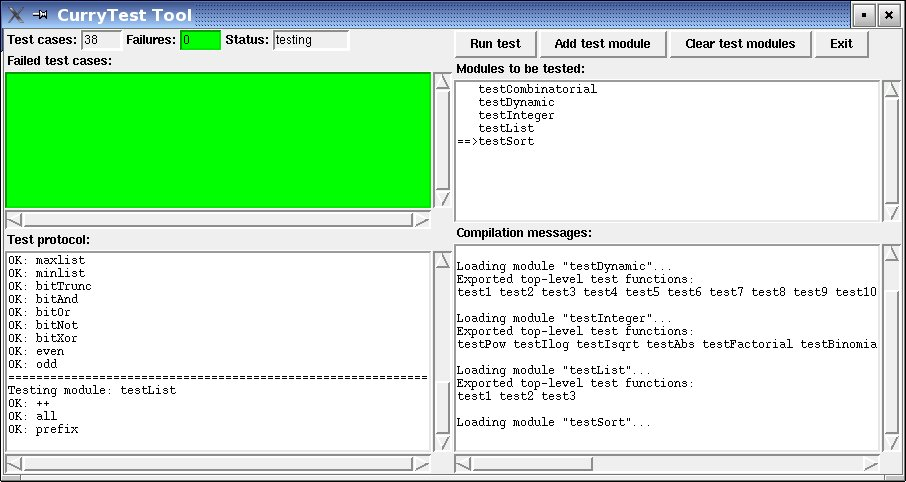
\includegraphics[scale=0.7]{currytest.jpg}
\end{center}
\caption{Snapshot of CurryTest's graphical interface\label{fig-currytest}}
\end{figure}


\newpage

\section{ERD2Curry: A Tool to Generate Programs from ER Specifications}
\label{sec-erd2curry}

ERD2Curry\index{ERD2Curry}\index{database programming}
is a tool to generate Curry code to access and manipulate data
persistently stored from
entity relationship diagrams.\index{entity relationship diagrams}
The idea of this tool is described in detail in
\cite{BrasselHanusMueller08PADL}.
Thus, we describe only the basic steps to use this tool
in the following.

If one creates an entity relationship diagram (ERD)
with the Umbrello UML Modeller, one has to store its
XML description in XMI format (as offered by Umbrello)
in a file, e.g., \ccode{myerd.xmi}.
This description can be compiled into a Curry program by the
command\pindex{erd2curry}
\startprog
erd2curry myerd.xmi
\stopprog
(\code{erd2curry} is a program stored in \code{$pakcshome$/bin}
where $pakcshome$ is the installation directory of PAKCS;
see Section~\ref{sec-general}).
If \code{MyData} is the name of the ERD, the Curry program file
\ccode{MyData.curry} is generated containing all the necessary
database access code as described in \cite{BrasselHanusMueller08PADL}.

If one does not want to use the Umbrello UML Modeller,
one can also create a textual description of the ERD
as a Curry term of type \code{ERD}
(w.r.t.\ the type definition given in module
\code{$pakcshome$/tools/erd2curry/ERD.curry})
and store it in some file, e.g., \ccode{myerd.term}.
This description can be compiled into a Curry program by the
command\pindex{erd2curry}
\startprog
erd2curry -t myerd.term
\stopprog
%
There is also the possibility to visualize an ERD term
as a graph with the graph visualization program \code{dotty}
(for this purpose, it might be necessary to adapt the definition
of the operation \code{dotCmd} in
\code{$pakcshome$/tools/erd2curry/ERD2Graph.curry}
according to your local environment).
This can be done by the command
\startprog
erd2curry -v myerd.term
\stopprog

\paragraph{Inclusion in the Curry application:}
To compile the generated database code, either
include the directory \code{$pakcshome$/tools/erd2curry}
into your Curry load path
(e.g., by setting  the environment variable
\ccode{CURRYPATH}\pindex{CURRYPATH}, see also Section~\ref{sec-modules})
or copy the file
\code{$pakcshome$/tools/erd2curry/ERDGeneric.curry}
into the directory of the generated database code.


\newpage

\section{UI: Declarative Programming of User Interfaces}
\label{sec-ui}

The PAKCS distribution contains a collection of libraries
to implement graphical user interfaces\index{user interface}
as well as web-based user interfaces
from declarative descriptions.
Exploiting these libraries, it is possible
to define the structure and functionality of a user interface
independent from the concrete technology.
Thus, a graphical user interface or a web-based user interface
can be generated from the same description by simply changing
the imported libraries.
This programming technique is described in detail in
\cite{HanusKluss09PADL}.

The libraries implementing these user interfaces are contained
in the directory
\startprog
$pakcshome$/tools/ui
\stopprog
Thus, in order to compile programs containing such user interface
specifications, one has to
include the directory \code{$pakcshome$/tools/ui}
into the Curry load path
(e.g., by setting  the environment variable
\ccode{CURRYPATH}\pindex{CURRYPATH}, see also Section~\ref{sec-modules}).
The directory
\startprog
$pakcshome$/tools/ui/examples
\stopprog
contains a few examples for such user interface specifications.


\newpage

\section{Preprocessing FlatCurry Files}
\label{sec-pakcspp}

The current parser allows to apply transformations on the intermediate
FlatCurry files after they are generated from the
corresponding Curry source file.
Currently, only the FlatCurry file corresponding to the main module
can be transformed.

A transformation can be specified as follows:
\begin{enumerate}
\item {\bf Options to \code{pakcs/bin/parsecurry}:}
\begin{description}
\item[\fbox{\code{--fpopt}}]\pindex{-fpopt}
Apply functional pattern optimization
(see \code{pakcs/tools/optimize/NonStrictOpt.curry} for details).

\item[\fbox{\code{--compact}}]\pindex{--compact}
Apply code compactification after parsing, i.e., transform the main
module and all its imported into one module and delete all
non-accessible functions.

\item[\fbox{\code{--compactexport}}]
Similar to \code{--compact} but delete all functions that are not accessible
from the exported functions of the main module.

\item[\fbox{\code{--compactmain:f}}]
Similar to \code{--compact} but delete all functions that are not accessible
from the function \ccode{f} of the main module.

\item[\fbox{\code{--fcypp cmd}}]\pindex{--fcypp}
Apply command \code{cmd} to the main module after parsing. This is useful to
integrate your own transformation into the compilation process.
Note that the command \ccode{cmd prog} should perform a transformation
on the FlatCurry file \code{prog.fcy}, i.e., it replaces the FlatCurry
file by a new one.
\end{description}

\item {\bf Setting the environment variable \code{FCYPP}:}\pindex{FCYPP}\\
For instance, setting \code{FCYPP} by
\startprog
export FCYPP="--fpopt"
\stopprog
will apply the functional pattern optimization if programs are compiled
and loaded in the PAKCS programming environment.


\item {\bf Putting options into the source code:}\pindex{PAKCS_OPTION_FCYPP}\\
If the source code contains a line with a comment of the form (the comment
must start at the beginning of the line)
\startprog
\{-\# PAKCS_OPTION_FCYPP <options> \#-\}
\stopprog
then the transformations specified by \code{<options>} are applied after
translating the source code into FlatCurry code. For instance,
the functional pattern optimization can be set by the comment
\startprog
\{-\# PAKCS_OPTION_FCYPP --fpopt \#-\}
\stopprog
in the source code. Note that this comment must be in a single line 
of the source program. If there are multiple lines containing such comments,
only the first one will be considered.
\end{enumerate}
\paragraph{Multiple options:}
Note that an arbitrary number of transformations can be specified
by the methods described above.
If several specifications for preprocessing FlatCurry files are used,
they are executed in the following order:
\begin{enumerate}
\item all transformations specified by the environemnt variable
\code{FCYPP} (from left to right)
\item all transformations specified as command line options of parsecurry
   (from left to right)
\item all transformations specified by a comment line in the source code
   (from left to right)
\end{enumerate}


\newpage

\section{Technical Problems}

Due to the fact that Curry is intended to implement
distributed systems (see Appendix~\ref{sec-ports}),
it might be possible that some technical problems
arise due to the use of sockets for implementing these
features. Therefore, this section gives some information
about the technical requirements of PAKCS and how to solve
problems due to these requirements.

There is one fixed port that is used by the implementation of PAKCS:
\begin{description}
\item[Port 8766:] This port is used by the
{\bf Curry Port Name Server} (CPNS) to implement symbolic names for
ports in Curry (see Appendix~\ref{sec-ports}).
If some other process uses this port on the machine,
the distribution facilities defined in the module \code{Ports}
(see Appendix~\ref{sec-ports}) cannot be used.
\end{description}
If these features do not work, you can try to find out
whether this port is in use by the shell command
\ccode{netstat -a | fgrep 8766} (or similar).

The CPNS is implemented as a demon listening on its port 8766
in order to serve requests about registering a new symbolic
name for a Curry port or asking the physical port number
of a Curry port. The demon will be automatically started for
the first time on a machine when a user compiles a program
using Curry ports. It can also be manually started and terminated by the
scripts \code{$pakcshome$/cpns/start} and
\code{$pakcshome$/cpns/stop}.
If the demon is already running, the command \code{$pakcshome$/cpns/start}
does nothing (so it can be always executed
before invoking a Curry program using ports).

If you detect any further technical problem,
please write to
\begin{center}
\code{mh@informatik.uni-kiel.de}
\end{center}

\newpage

\addcontentsline{toc}{section}{Bibliography}
\bibliography{manual}
\bibliographystyle{plain}

\newpage
\appendix

\section{Libraries of the PAKCS Distribution}
\label{sec:libraries}

{\setlength{\parindent}{0.0cm}

The PAKCS compiler system provides an extensive collection
of libraries for application programming.
The libraries for arithmetic constraints over real numbers,
finite domain constraints,
ports for concurrent and distributed programming, and
meta-programming by representing Curry programs in Curry
are described in the following subsection in more detail.
The complete set of libraries with all exported types and functions
are described in the further subsections.
For a more detailed online documentation of all libraries of PAKCS,
see \url{http://www.informatik.uni-kiel.de/~pakcs/lib/index.html}.

\subsection{Constraints, Ports, Meta-Programming}

\subsubsection{Arithmetic Constraints}

The primitive entities for the use of arithmetic constraints
are defined in the system module \code{CLPR}
(cf.\ Section~\ref{sec-modules}), i.e., in order to use them,
the program must contain the import declaration
\startprog
import CLPR
\stopprog
Floating point arithmetic is supported in PAKCS
via arithmetic constraints, i.e., the equational constraint
\ccode{2.3 +.~x =:= 5.5} is solved by binding \code{x} to \code{3.2}
(rather than suspending the evaluation of the addition,
as in corresponding constraints on integers like
\ccode{3+x=:=5}). All operations related to
floating point numbers are suffixed by \ccode{.}.
The following functions and constraints on floating point
numbers are supported in PAKCS:
\begin{description}
\item[\code{(+.)   :: Float -> Float -> Float}]~\\
Addition on floating point numbers.
\item[\code{(-.)   :: Float -> Float -> Float}]~\\
Subtraction on floating point numbers.
\item[\code{(*.)   :: Float -> Float -> Float}]~\\
Multiplication on floating point numbers.
\item[\code{(/.)   :: Float -> Float -> Float}]~\\
Division on floating point numbers.
\item[\code{(<.)   :: Float -> Float -> Success}]~\\
Comparing two floating point numbers with the ``less than'' relation.
\item[\code{(>.)   :: Float -> Float -> Success}]~\\
Comparing two floating point numbers with the ``greater than'' relation.
\item[\code{(<=.)  :: Float -> Float -> Success}]~\\
Comparing two floating point numbers with the ``less than or equal'' relation.
\item[\code{(>=.)  :: Float -> Float -> Success}]~\\
Comparing two floating point numbers with the ``greater than or equal''
relation.
\item[\code{i2f    :: Int -> Float}]~\\
Converting an integer number into a floating point number.
\end{description}
As an example, consider a constraint \code{mortgage}
which relates the principal \code{p},
the lifetime of the mortgage in months \code{t},
the monthly interest rate \code{ir},
the monthly repayment \code{r},
and the outstanding balance at the end of the lifetime \code{b}.
The financial calculations
can be defined by the following two rules in Curry (the second rule
describes the repeated accumulation of the interest):
\startprog
~
import CLPR
~
mortgage p t ir r b | t >. 0.0 \& t <=. 1.0  --lifetime not more than 1 month?
                    =  b =:= p *. (1.0 +. t *. ir) -. t*.r \vspace{1ex}
mortgage p t ir r b | t >. 1.0               --lifetime more than 1 month?
                    =  mortgage (p *. (1.0+.ir)-.r) (t-.1.0) ir r b
~
\stopprog
Then we can calculate the monthly payment for paying back
a loan of \$100,000 in 15 years with a monthly interest rate of 1\%
by solving the goal
\startprog
mortgage 100000.0 180.0 0.01 r 0.0
\stopprog
which yields the solution \code{r=1200.17}.

Note that only linear arithmetic equalities or inequalities
are solved by the constraint solver. Non-linear constraints
like \ccode{x *.~x =:= 4.0} are suspended until they become
linear.


\subsubsection{Finite Domain Constraints}

Finite domain constraints are constraints where all variables
can only take a finite number of possible values.
For simplicity, the domain of finite domain variables are
identified with a subset of the integers, i.e., the type
of a finite domain variable is \code{Int}. The arithmetic
operations related to finite domain variables are suffixed by \ccode{\#}.
The following functions and constraints for finite domain constraint solving
are currently supported in PAKCS:\footnote{Note that
this library is based on the corresponding library of SICStus-Prolog
but does not implement the complete functionality of the SICStus-Prolog library.
However, using the PAKCS interface for external functions (see
Appendix~\ref{sec-external-functions}), it is relatively
easy to provide the complete functionality.}

\begin{description}
\item[\code{domain :: [Int] -> Int -> Int -> Success}]~\\
The constraint \ccode{domain [$x_1,\ldots,x_n$] $l$ $u$}
is satisfied if the domain of all variables $x_i$ is the interval $[l,u]$.
\item[\code{(+\#)   :: Int -> Int -> Int}]~\\
Addition on finite domain values.
\item[\code{(-\#)   :: Int -> Int -> Int}]~\\
Subtraction on finite domain values.
\item[\code{(*\#)   :: Int -> Int -> Int}]~\\
Multiplication on finite domain values.
\item[\code{(=\#)   :: Int -> Int -> Success}]~\\
Equality of finite domain values.
\item[\code{(/=\#)  :: Int -> Int -> Success}]~\\
Disequality of finite domain values.
\item[\code{(<\#)   :: Int -> Int -> Success}]~\\
``less than'' relation on finite domain values.
\item[\code{(<=\#)  :: Int -> Int -> Success}]~\\
``less than or equal'' relation on finite domain values.
\item[\code{(>\#)   :: Int -> Int -> Success}]~\\
``greater than'' relation on finite domain values.
\item[\code{(>=\#)  :: Int -> Int -> Success}]~\\
``greater than or equal'' relation on finite domain values.
\item[\code{sum :: [Int] -> (Int -> Int -> Success) -> Int -> Success}]~\\
The constraint \ccode{sum [$x_1,\ldots,x_n$] $op$ $x$}
is satisfied if all $x_1+\cdots + x_n \mathrel{op} x$ is satisfied,
where $op$ is one of the above finite domain constraint relations
(e.g., \ccode{=\#}).
\item[\code{scalar_product :: [Int] -> [Int] -> (Int -> Int -> Success) -> Int -> Success}]~\\
The constraint \ccode{scalar_product [$c_1,\ldots,c_n$] [$x_1,\ldots,x_n$] $op$ $x$}
is satisfied if all $c_1 x_1+\cdots + c_n x_n \mathrel{op} x$ is satisfied,
where $op$ is one of the above finite domain constraint relations.
\item[\code{count :: Int -> [Int] -> (Int -> Int -> Success) -> Int -> Success}]~\\
The constraint \ccode{count $k$ [$x_1,\ldots,x_n$] $op$ $x$}
is satisfied if all $k \mathrel{op} x$ is satisfied,
where $n$ is the number of the $x_i$ that are equal to $k$ and
$op$ is one of the above finite domain constraint relations.
\item[\code{all_different :: [Int] -> Success}]~\\
The constraint \ccode{all_different [$x_1,\ldots,x_n$]}
is satisfied if all $x_i$ have pairwise different values.
\item[\code{labeling :: [LabelingOption] -> [Int] -> Success}]~\\
The constraint \ccode{labeling $os$ [$x_1,\ldots,x_n$]}
non-deterministically instantiates all $x_i$ to the values
of their domain according to the options $os$ (see the module documentation
for further details about these options).
\end{description}
These entities are defined in the system module \code{CLPFD}
(cf.\ Section~\ref{sec-modules}), i.e., in order to use it,
the program must contain the import declaration
\startprog
import CLPFD
\stopprog
As an example, consider the classical \ccode{send+more=money} problem
where each letter must be replaced by a different digit such that this
equation is valid and there are no leading zeros.
The usual way to solve finite domain constraint problems
is to specify the domain of the involved variables followed
by a specification of the constraints and the labeling
of the constraint variables in order to start the search for solutions.
Thus, the \ccode{send+more=money} problem can be solved as follows:
\startprog
~
import CLPFD
~
smm l =
        l =:= [s,e,n,d,m,o,r,y] \&
        domain l 0 9 \&
        s >\# 0 \&
        m >\# 0 \&
        all_different l  \&
                         1000 *\# s +\# 100 *\# e +\# 10 *\# n +\# d
        +\#               1000 *\# m +\# 100 *\# o +\# 10 *\# r +\# e
        =\# 10000 *\# m +\# 1000 *\# o +\# 100 *\# n +\# 10 *\# e +\# y \&
        labeling [FirstFail] l
        where s,e,n,d,m,o,r,y free
~
\stopprog
Then we can solve this problem by evaluating the goal
\ccode{smm [s,e,n,d,m,o,r,y]} which yields the unique solution
\code{\{s=9,e=5,n=6,d=7,m=1,o=0,r=8,y=2\}}.


\subsubsection{Ports: Distributed Programming in Curry}
\label{sec-ports}

To support the development of concurrent and distributed applications,
PAKCS supports internal and external ports\index{ports} as
described in \cite{Hanus99PPDP}.
Since \cite{Hanus99PPDP} contains a detailed description of this
concept together with various programming examples, we only summarize here
the functions and constraints supported for ports in PAKCS.

The basic datatypes, functions, and constraints for ports
are defined in the system module \code{Ports}
(cf.\ Section~\ref{sec-modules}), i.e., in order to use ports,
the program must contain the import declaration
\startprog
import Ports
\stopprog
This declaration includes the following entities in the program:
\begin{description}
\item[\code{Port a}\pindex{Port}]~\\
This is the datatype of a port to which one can send messages of type \code{a}.

\item[\code{openPort :: Port a -> [a] -> Success}]~\\
The constraint \ccode{openPort p s}\pindex{openPort}
establishes a new \emph{internal port}
\code{p} with an associated message stream \code{s}. \code{p} and \code{s} must be
unbound variables,
otherwise the constraint fails (and causes a runtime error).

\item[\code{send :: a -> Port a -> Success}]~\\
The constraint \ccode{send m p}\pindex{send}
is satisfied if \code{p} is constrained
to contain the message \code{m}, i.e., \code{m} will be sent to the port
\code{p} so that it appears in the corresponding stream.

\item[\code{doSend :: a -> Port a -> IO ()}]~\\
The I/O action \ccode{doSend m p}\pindex{doSend} solves the constraint
\ccode{send m p} and returns nothing.

\item[\code{openNamedPort :: String -> IO [a]}]~\\
The I/O action \ccode{openNamedPort n}\pindex{openNamedPort}
opens a new \emph{external port} with
symbolic name \code{n} and returns the associated stream of messages.

\item[\code{connectPort :: String -> IO (Port a)}]~\\
The I/O action \ccode{connectPort n}\pindex{connectPort}
returns a port with symbolic name
\code{n} (i.e., \code{n} must have the form ``\emph{portname@machine})
to which one can send messages by the \code{send} constraint.
Currently, no dynamic type checking is done for external ports,
i.e., sending messages of the wrong type to a port might lead to
a failure of the receiver.
\end{description}

\paragraph{Restrictions:}
Every expression, possibly containing logical variables, can be sent to
a port. However, as discussed in \cite{Hanus99PPDP},
port communication is strict, i.e., the expression is
evaluated to normal form before sending it by the
constraint \code{send}. Furthermore, if messages containing
logical variables are sent to \emph{external ports},
the behavior is as follows:
\begin{enumerate}
\item The sender waits until all logical variables in the message
have been bound by the receiver.
\item The binding of a logical variable received by a process
is sent back to the sender of this logical variable only if
it is bound to a \emph{ground} term, i.e., as long as the binding contains
logical variables, the sender is not informed about the binding
and, therefore, the sender waits.
\end{enumerate}

\paragraph{External ports on local machines:}
The implementation of external ports assumes that the
host machine running the application is connected to the Internet
(i.e., it uses the standard IP address of the host machine
for message sending). If this is not the case and the application
should be tested by using external ports only on the local host
without a connection to the Internet,
the environment variable \ccode{PAKCS_LOCALHOST}\pindex{PAKCS_LOCALHOST}
must be set to \ccode{yes}
\emph{before PAKCS system is started}.
In this case, the IP address \code{127.0.0.1} and the hostname
\ccode{localhost} are used for identifying the local machine.

\paragraph{Selection of Unix sockets for external ports:}
The implementation of ports uses sockets to communicate
messages sent to external ports.
Thus, if a Curry program uses the
I/O action \code{openNamedPort}\pindex{openNamedPort}
to establish an externally visible server,
PAKCS selects a Unix socket for the port communication.
Usually, a free socket is selected by the operating system.
If the socket number should be fixed in an application (e.g.,
because of the use of firewalls\index{firewall} that allow only
communication over particular sockets), then one
can set the environment variable \ccode{PAKCS_SOCKET}\pindex{PAKCS_SOCKET}
to a distinguished socket number before the PAKCS system is started.
This has the effect that PAKCS uses only this socket
number for communication (even for several external ports
used in the same application program).

\paragraph{Debugging:}
To debug distributed systems,
it is sometimes helpful to see all messages sent to external ports.
This is supported by the environment variable
\ccode{PAKCS_TRACEPORTS}.\pindex{PAKCS_TRACEPORTS}
If this variable is set to \ccode{yes}
\emph{before the PAKCS system is started}, then all
connections to external ports and all
messages sent and received on external ports are
printed on the standard error stream.


\subsubsection{AbstractCurry and FlatCurry: Meta-Programming in Curry}
\label{sec-flatcurry}

\index{AbstractCurry}
\index{FlatCurry}
To support meta-programming, i.e., the manipulation of Curry programs
in Curry, there are system modules \code{FlatCurry} and \code{AbstractCurry}
(stored in the directory \ccode{$pakcshome$/lib/meta})
which define datatypes for the representation
of Curry programs.
\code{AbstractCurry} is a more direct representation of a Curry program,
whereas \code{FlatCurry} is a simplified representation
where local function definitions are replaced by global definitions
(i.e., lambda lifting has been performed) and pattern matching
is translated into explicit case/or expressions.
Thus, \code{FlatCurry} can be used for more back-end oriented
program manipulations (or, for writing new back ends for Curry),
whereas \code{AbstractCurry} is intended for manipulations of
programs that are more oriented towards the source program.

Both modules contain predefined I/O actions to read programs
in the \code{AbstractCurry} (\code{readCurry}\pindex{readCurry})
or \code{FlatCurry}
(\code{readFlatCurry}\pindex{readFlatCurry}) format.
These actions parse the corresponding source program and return
a data term representing this program (according to the definitions
in the modules \code{AbstractCurry} and \code{FlatCurry}).

Since all datatypes are explained in detail in these modules,
we refer to the online documentation\footnote{%
\url{http://www.informatik.uni-kiel.de/~pakcs/lib/CDOC/FlatCurry.html} and
\url{http://www.informatik.uni-kiel.de/~pakcs/lib/CDOC/AbstractCurry.html}}
of these modules.

As an example, consider a program file \ccode{test.curry}
containing the following two lines:
\startprog
rev []     = []
rev (x:xs) = (rev xs) ++ [x]
\stopprog
Then the I/O action \code{(FlatCurry.readFlatCurry "test")} returns the
following term:
\startprog
 (Prog "test"
  ["Prelude"]
  []
  [Func ("test","rev") 1 Public
        (FuncType (TCons ("Prelude","[]") [(TVar 0)])
                  (TCons ("Prelude","[]") [(TVar 0)]))
        (Rule [0]
           (Case Flex (Var 0)
              [Branch (Pattern ("Prelude","[]") [])
                  (Comb ConsCall ("Prelude","[]") []),
               Branch (Pattern ("Prelude",":") [1,2])
                  (Comb FuncCall ("Prelude","++")
                        [Comb FuncCall ("test","rev") [Var 2],
                         Comb ConsCall ("Prelude",":")
                              [Var 1,Comb ConsCall ("Prelude","[]") []]
                        ])
              ]))]
  []
 )
\stopprog


%%%%%%%%%%%%%%%%%%%%%%%%%%%%%%%%%%%%%%%%%%%%%%%%%%%%%%%%%%%%%%%%%%%%%%%%%
% Definitions in order to LaTeX documents generated by "currydoc --tex"
%%%%%%%%%%%%%%%%%%%%%%%%%%%%%%%%%%%%%%%%%%%%%%%%%%%%%%%%%%%%%%%%%%%%%%%%%

\newcommand{\currymodule}[1]{\subsubsection{Library #1}\label{Library:#1}}
\newcommand{\currytypesstart}{\subsubsection*{Exported types:}}
\newcommand{\currytypesstop}{}
\newcommand{\currytypesynstart}[2]{{\tt type #2}\pindex{#1} \begin{quote}}
\newcommand{\currytypesynstop}{\end{quote}}
\newcommand{\currydatastart}[1]{{\tt data #1}\pindex{#1} \begin{quote}}
\newcommand{\currydatacons}{\end{quote}%
\begin{itemize}\item[] \hspace{-4ex}\emph{Exported constructors:}}
\newcommand{\currydatastop}{\end{itemize}}
\newcommand{\curryconsstart}[2]{\item {\tt #1~::~#2}\par}
\newcommand{\curryfuncstart}{\subsubsection*{Exported functions:}}
\newcommand{\curryfuncstop}{}
\newcommand{\curryfunctionstart}[2]{#2\pindex{#1}\begin{quote}}
\newcommand{\curryfunctionstop}{\end{quote}}
\newcommand{\curryfuncsig}[2]{{\tt #1~::~#2}}


\subsection{General Libraries}

\input{lib/AllSolutions}
\input{lib/Assertion}
\input{lib/Char}
\input{lib/CLPFD}
\input{lib/CLPR}
\input{lib/CLPB}
\input{lib/Combinatorial}
\input{lib/Constraint}
\input{lib/CSV}
\input{lib/Database}
\input{lib/DaVinci}
\input{lib/Directory}
\input{lib/Dynamic}
\input{lib/FileGoodies}
\input{lib/Float}
\input{lib/Global}
\input{lib/GlobalVariable}
\input{lib/GUI}
\input{lib/Integer}
\input{lib/IO}
\input{lib/IOExts}
\input{lib/JavaScript}
\input{lib/KeyDatabase}
\input{lib/KeyDatabaseSQLite}
\input{lib/KeyDB}
\input{lib/List}
\input{lib/Maybe}
\input{lib/NamedSocket}
\input{lib/Parser}
\input{lib/Ports}
\input{lib/Pretty}
\input{lib/Profile}
\input{lib/PropertyFile}
\input{lib/Read}
\input{lib/ReadNumeric}
\input{lib/ReadShowTerm}
\input{lib/SetFunctions}
\input{lib/Socket}
\input{lib/System}
\input{lib/Time}
%\input{lib/Tk}
\input{lib/Unsafe}


\subsection{Data Structures and Algorithms}

\input{lib/Array}
\input{lib/Dequeue}
\input{lib/FiniteMap}
\input{lib/GraphInductive}
\input{lib/Random}
\input{lib/RedBlackTree}
\input{lib/SetRBT}
\input{lib/Sort}
\input{lib/TableRBT}
\input{lib/Traversal}

\subsection{Libraries for Web Applications}

\input{lib/CategorizedHtmlList}
\input{lib/HTML}
\input{lib/HtmlParser}
\input{lib/Mail}
\input{lib/Markdown}
\input{lib/WUI}
\input{lib/URL}
\input{lib/XML}
\input{lib/XmlConv}

\subsection{Libraries for Meta-Programming}

\input{lib/AbstractCurry}
\input{lib/AbstractCurryPrinter}
\input{lib/CompactFlatCurry}
\input{lib/CurryStringClassifier}
\input{lib/FlatCurry}
\input{lib/FlatCurryGoodies}
\input{lib/FlatCurryRead}
\input{lib/FlatCurryShow}
\input{lib/FlatCurryTools}
\input{lib/FlatCurryXML}
\input{lib/FlexRigid}
\input{lib/PrettyAbstract}

} % end setlength parindent

\newpage

\input{markdown_syntax}

\newpage

\begin{figure}%[t]
\begin{center}
 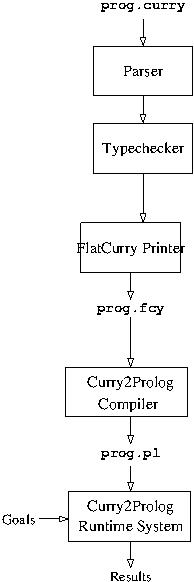
\includegraphics[scale=0.85]{pakcs_overview.jpg}
\end{center}\vspace{-5ex}
\caption{Overview of PAKCS\label{fig-pakcs}}
\end{figure}

\section{Overview of the PAKCS Distribution}

A schematic overview of the various components contained in
the distribution of PAKCS and the
translation process of programs inside PAKCS is shown in
Figure~\ref{fig-pakcs} on page~\pageref{fig-pakcs}.
In this figure, boxes denote different components of PAKCS
and names in boldface denote files containing
various intermediate representations during the translation
process (see Section~\ref{sec-auxfiles} below).
The PAKCS distribution contains a front end for reading (parsing and
type checking) Curry programs that can be also used by
other Curry implementations.
The back end (formerly known as ``Curry2Prolog''\index{Curry2Prolog})
compiles Curry programs into Prolog programs.
It also support constraint solvers for
arithmetic constraints over real numbers and finite domain constraints,
and further libraries for GUI programming, meta-programming etc.
Currently, it does not implement encapsulated search in full generality
(only a strict version of \code{findall} is supported),
and concurrent threads are not executed in a fair manner.


\newpage

\section{Auxiliary Files}
\label{sec-auxfiles}

During the translation and execution of a Curry program with PAKCS,
various intermediate representations of the source program are created
and stored in different files which are shortly explained in this section.
If you use the PAKCS, it is not necessary to know about
these auxiliary files because they are automatically generated
and updated. You should only remember the command for deleting
all auxiliary files (\ccode{cleancurry}, see Section~\ref{sec-general})
to clean up your directories.

The various components of PAKCS create
the following auxiliary files.
\begin{description}
\item[\code{prog.fcy}:] This file contains the Curry program
in the so-called ``FlatCurry'' representation where all functions are global
(i.e., lambda lifting has been performed) and pattern matching
is translated into explicit case/or expressions
(compare Appendix~\ref{sec-flatcurry}).
This representation might be useful for other back ends and
compilers for Curry and is the basis doing meta-programming in Curry.
This file is implicitly
generated when a program is read by PAKCS.
It can be also explicitly generated by the command\pindex{parsecurry}
\startprog
parsecurry --flat prog
\stopprog
The FlatCurry representation of a Curry program is usually
generated by the front-end after parsing, type checking and eliminating
local declarations.
If $dir$ is the directory where the Curry program is stored,
the corresponding FlatCurry program is stored in the directory
\ccode{$dir$/.curry}.

\item[\code{prog.fint}:] This file contains the interface
of the program in the so-called ``FlatCurry'' representation,
i.e., it is similar to \code{prog.fcy} but contains only exported
entities and the bodies of all functions omitted (i.e., ``external'').
This representation is useful for providing a fast access
to module interfaces.
This file is implicitly generated by the command\pindex{parsecurry}
\startprog
parsecurry --flat prog
\stopprog
and stored in the same directory as \code{prog.fcy}.

\item[\code{prog.pl}:] This file contains a Prolog program
as the result of translating the Curry program with PAKCS.
If $dir$ is the directory where the Curry program is stored,
the corresponding Prolog program is stored in the directory
\ccode{$dir$/.curry/.pakcs}.

\item[\code{prog.po}:] This file contains the Prolog program
\code{prog.pl} in an intermediate format for faster loading.
This file is stored in the same directory as \code{prog.pl}.

\item[\code{prog.state}:] This file contains the saved state
after compiling and saving a program with PAKCS
(see Section~\ref{sec-use-curry2prolog}).

\end{description}


\newpage


\section{Changing the Prelude or System Modules}

The standard prelude, which is automatically imported into each Curry program,
and all system modules containing datatypes and functions
useful for application programming
(cf.\ Appendix~\ref{sec:libraries})
are stored in the system module directory \ccode{$pakcshome$/lib}
(and its subdirectories).
If you change any of these modules,
you have to recompile the complete system by
executing \code{make} in the directory $pakcshome$.



\newpage

\section{External Functions}
\label{sec-external-functions}

\index{function!external}\index{external function}
Currently, PAKCS has no general interface to external functions.
Therefore, if a new external function should be added
to the system, this function must be declared as \code{external}
in the Curry source code
and then an implementation for this external function
must be inserted in the corresponding back end.
An external function is defined as follows in the Curry source code:
\begin{enumerate}
\item
Add a type declaration for the external function somewhere
in the body of the appropriate file (usually, the prelude
or some system module).
\item
For external functions it is not allowed to define any
rule since their semantics is determined by an external implementation.
Instead of the defining rules, you have to write
\startprog
f external
\stopprog
somewhere in the file containing the type declaration for 
the external function \code{f}.
\end{enumerate}
For instance, the addition on integers can be declared as
an external function as follows:
\startprog
(+) :: Int -> Int -> Int
(+) external
\stopprog
The further modifications to be done for an inclusion of
an external function has to be done in the back end.
A new external function is added to the back end of PAKCS
by informing the compiler about the existence of an external function
and adding an implementation of this function in the run-time
system. Therefore, the following items must be added
in the PAKCS compiler system:
\begin{enumerate}
\item
If the Curry module \code{Mod} contains external functions,
there must be a file named \code{Mod.prim_c2p} containing the
specification of these external functions. The contents of this file
is in XML format and has the following general structure:\footnote{%
\url{http://www.informatik.uni-kiel.de/~pakcs/primitives.dtd} contains a DTD
describing the exact structure of these files.}
\startprog
<primitives>
  \emph{specification of external function $f_1$}
  \ldots
  \emph{specification of external function $f_n$}
</primitives>
\stopprog
The specification of an external function $f$
with arity $n$ has the form
\startprog
<primitive name="$f$" arity="$n$">
  <library>lib</library>
  <entry>pred</entry>
</primitive>
\stopprog
where \code{lib} is the Prolog library (stored in the directory of the
Curry module or in the global directory
\code{$pakcshome$/curry2prolog/lib_src}) containing the code implementing this
function and \code{pred} is a predicate name in this library
implementing this function. Note that the function $f$ must be
declared in module \code{Mod}: either as an external function
or defined in Curry by equations. In the latter case,
the Curry definition is not translated but calls to this function
are redirected to the Prolog code specified above.

Furthermore, the list of specifications can also contain entries of the form
\startprog
<ignore name="$f$" arity="$n$" />
\stopprog
for functions $f$ with arity $n$ that are declared in module \code{Mod}
but should be ignored for code generation, e.g., since they are
never called w.r.t.\ to the current implementation of external functions.
For instance, this is useful when functions that can
be defined in Curry should be (usually more efficiently) are implemented
as external functions.

Note that the arguments are passed in their current (possibly unevaluated) form.
Thus, if the external function requires the arguments to be evaluated
in a particular form, this must be done before calling the external function.
For instance, the external function for adding two integers
requires that both arguments must be evaluated to non-variable head normal form
(which is identical to the ground constructor normal form). Therefore,
the function \ccode{+} is specified in the prelude by
\startprog
(+)   :: Int -> Int -> Int
x + y = (prim_Int_plus \$\# y) \$\# x
\medskip
prim_Int_plus :: Int -> Int -> Int
prim_Int_plus external
\stopprog
where \code{prim_Int_plus} is the actual external function implementing
the addition on integers. Consequently, the specification file
\code{Prelude.prim_c2p} has an entry of the form
\startprog
<primitive name="prim_Int_plus" arity="2">
  <library>prim_standard</library>
  <entry>prim_Int_plus</entry>
</primitive>
\stopprog
where the Prolog library \code{prim_standard.pl} contains the Prolog code
implementing this function.

\item
For most external functions, a \emph{standard interface} is
generated by the compiler so that an $n$-ary function can be
implemented by an $(n+1)$-ary predicate where the last argument must
be instantiated to the result of evaluating the function.  The
standard interface can be used if all arguments are ensured to be
fully evaluated (e.g., see definition of \code{(+)} above) and no
suspension control is necessary, i.e., it is ensured that the
external function call does not suspend for all arguments.
Otherwise, the raw interface (see below) must be used.  For
instance, the Prolog code implementing \code{prim_Int_plus}
contained in the Prolog library \code{prim_standard.pl} is as
follows (note that the arguments of \code{(+)} are passed in reverse
order to \code{prim_Int_plus} in order to ensure a left-to-right
evaluation of the original arguments by the calls to \code{(\$\#)}):
\startprog
prim_Int_plus(Y,X,R) :- R is X+Y.
\stopprog

\item
The \emph{standard interface for I/O actions}, i.e., external functions
with result type \code{IO~a}, assumes that the I/O action
is implemented as a predicate (with a possible side effect)
that instantiates the last argument to the returned value of type \ccode{a}.
For instance, the primitive predicate \code{prim_getChar}
implementing prelude I/O action \code{getChar}
can be implemented by the Prolog code
\startprog
prim_getChar(C) :- get_code(N), char_int(C,N).
\stopprog
where \code{char_int} is a predicate relating the internal
Curry representation of a character with its ASCII value.

\item
If some arguments passed to the external functions are not fully evaluated
or the external function might suspend, the implementation must follow
the structure of the PAKCS run-time system by using
the \emph{raw interface}. In this case, the name of the external entry
must be suffixed by \ccode{[raw]} in the \code{prim_c2p} file.
For instance, if we want to use the raw interface for the external function
\code{prim_Int_plus},
the specification file \code{Prelude.prim_c2p} must have an entry of the form
\startprog
<primitive name="prim_Int_plus" arity="2">
  <library>prim_standard</library>
  <entry>prim_Int_plus[raw]</entry>
</primitive>
\stopprog
In the raw interface, the actual implementation of an $n$-ary external function consists
of the definition of an $(n+3)$-ary predicate $pred$.
The first $n$ arguments are the corresponding actual arguments.
The $(n+1)$-th argument is a free variable which must be
instantiated to the result of the function call after
successful execution. The last two arguments
control the suspension behavior of the function
(see \cite{AntoyHanus00FROCOS} for more details):
The code for the predicate $pred$
should only be executed when the $(n+2)$-th argument
is not free, i.e., this predicate has always the
SICStus-Prolog block declaration
\startprog
?- block $pred$(?,\ldots,?,-,?).
\stopprog
In addition, typical external functions should suspend
until the actual arguments are instantiated. This can be ensured
by a call to \code{ensureNotFree} or \code{(\$\#)}
before calling the external function. Finally, the
last argument (which is a free variable at call time)
must be unified with the $(n+2)$-th argument
after the function call is successfully evaluated
(and does not suspend). Additionally, the actual (evaluated) arguments
must be dereferenced before they are accessed.
Thus, an implementation
of the external function for adding integers is as follows in the raw interface:
\startprog
?- block prim_Int_plus(?,?,?,-,?).
prim_Int_plus(RY,RX,Result,E0,E) :-
     deref(RX,X), deref(RY,Y), Result is X+Y, E0=E.
\stopprog
Here, \code{deref} is a predefined predicate for dereferencing the
actual argument into a constant (and \code{derefAll} for dereferencing
complex structures).
\end{enumerate}
%
The Prolog code implementing the external functions must be accessible to the run-time
system of PAKCS by putting it into the directory containing the corresponding
Curry module or into the system directory
\code{$pakcshome$/curry2prolog/lib_src}.
Then it will be automatically loaded into the run-time environment
of each compiled Curry program.

Note that arbitrary functions implemented in C or Java can be connected to
PAKCS by using the corresponding interfaces of underlying Prolog system.


\newpage
\addcontentsline{toc}{section}{Index}
\printindex


\end{document}

\clearpage
\documentclass[11pt,fleqn]{article}

\usepackage{latexsym}
\usepackage{makeidx}
\usepackage{url}
\usepackage{xspace}
\usepackage{graphicx}

\input{version}

%%% ------------------------------------------------------------------

\usepackage[colorlinks,linkcolor=blue]{hyperref}
\hypersetup{bookmarksopen=true}
\hypersetup{bookmarksopenlevel=0}
\hypersetup{pdftitle={PAKCS: The Portland Aachen Kiel Curry System}}
\hypersetup{pdfauthor={Michael Hanus}}
%\hypersetup{pdfstartview=Title}
\hypersetup{pdfstartview=FitH}
\usepackage{thumbpdf}

%%% ------------------------------------------------------------------

\setlength{\textwidth}{16.5cm}
\setlength{\textheight}{23cm}
\renewcommand{\baselinestretch}{1.1}
\setlength{\topmargin}{-1cm}
\setlength{\oddsidemargin}{0cm}
\setlength{\evensidemargin}{0cm}
\setlength{\marginparwidth}{0.0cm}
\setlength{\marginparsep}{0.0cm}

\newlength{\figurewidth}
\setlength{\figurewidth}{\textwidth}
\addtolength{\figurewidth}{-0.4cm}

% font for program texts
\renewcommand{\tt}{\usefont{OT1}{cmtt}{m}{n}\selectfont}
\newcommand{\codefont}{\tt}

% environment for typing program texts:
\makeatletter
\newenvironment{prog}{\par\vspace{0.7ex}
\setlength{\parindent}{1.0cm}
\setlength{\parskip}{-0.1ex}
\obeylines\@vobeyspaces\tt}{\vspace{0.7ex}\noindent
}
\makeatother
\newcommand{\startprog}{\begin{prog}}
\newcommand{\stopprog}{\end{prog}\noindent}

% program text in normal text
\newcommand{\code}[1]{\mbox{\codefont #1}}

% program text in normal text with apostrophs
\newcommand{\ccode}[1]{``\mbox{\codefont #1}''}

\newcommand{\pindex}[1]{\index{#1@{\tt #1}}}  % program elements in index

\newcommand{\labs}{\mbox{\tt\char92}}  % lambda abstraction in Curry
\newcommand{\todo}[1]{\fbox{\sc To do: #1}}
\newcommand{\cb}{CurryBrowser\xspace}

% allow underscores in programs:
\catcode`\_=\active
\let_=\sb
\catcode`\_=12

% produce an index:
\makeindex

\begin{document}
\sloppy

\begin{titlepage}
\pdfbookmark[1]{Title}{Title}
\begin{center}
\fbox{
\begin{minipage}[t]{\figurewidth}
\begin{center}\vspace{10ex}
{\Huge\bf PAKCS \pakcsversion}\\[4ex]
{\huge The Portland Aachen Kiel Curry System}\\[7ex]
{\huge User Manual}\\[4ex]
\pakcsversiondate\\[6ex]
\Large
Michael Hanus$^1$ [editor] \\[3ex]
{\large Additional Contributors:}\\[2ex]
Sergio Antoy$^2$ \\
Bernd Bra\ss{}el$^3$ \\
Martin Engelke$^4$ \\
Klaus H\"oppner$^5$ \\
Johannes Koj$^6$ \\
Philipp Niederau$^7$ \\
Ramin Sadre$^8$ \\
Frank Steiner$^9$ \\[4ex]
\normalsize
(1) University of Kiel, Germany, {\tt mh@informatik.uni-kiel.de} \\
(2) Portland State University, USA, {\tt antoy@cs.pdx.edu} \\
(3) University of Kiel, Germany, {\tt bbr@informatik.uni-kiel.de} \\
(4) University of Kiel, Germany, {\tt men@informatik.uni-kiel.de} \\
(5) University of Kiel, Germany, {\tt klh@informatik.uni-kiel.de} \\
(6) RWTH Aachen, Germany, {\tt johannes.koj@sdm.de} \\
(7) RWTH Aachen, Germany, {\tt philipp@navigium.de} \\
(8) RWTH Aachen, Germany, {\tt ramin@lvs.informatik.rwth-aachen.de} \\
(9) LMU Munich, Germany, {\tt fst@bio.informatik.uni-muenchen.de} \\[5ex]~
\end{center}
\end{minipage}}
\end{center}
\end{titlepage}

\pdfbookmark[1]{Contents}{Contents}
\tableofcontents

\newpage

\addcontentsline{toc}{section}{Preface}
\section*{Preface}

This document describes PAKCS (formerly called ``PACS''),
an implementation of the multi-paradigm language Curry,
jointly developed at the University of Kiel, the Technical University
of Aachen and Portland State University.
Curry is a universal programming language aiming at the amalgamation
of the most important declarative programming paradigms,
namely functional programming and logic programming.  
Curry combines in a seamless way features from functional programming
(nested expressions, lazy evaluation, higher-order functions),
logic programming (logical variables, partial data structures,
built-in search), and concurrent programming (concurrent evaluation
of constraints with synchronization on logical variables).
Moreover, the PAKCS implementation of Curry also supports
the high-level implementation of distributed applications,
graphical user interfaces, and web services
(as described in more detail in \cite{Hanus99PPDP,Hanus00PADL,Hanus01PADL}).

We assume familiarity with the ideas and features
of Curry as described in the Curry language definition \cite{Hanus12Curry}.
Therefore, this document only explains the use of the different
components of PAKCS
and the differences and restrictions of PAKCS
(see Section~\ref{sec-restrictions})
compared with the language Curry (Version 0.8.3).


\bigskip

\subsection*{Acknowledgements}

This work has been supported in part by the DAAD/NSF grant INT-9981317,
the NSF grants CCR-0110496 and CCR-0218224,
the Acci\'on Integrada hispano-alemana HA1997-0073,
and the DFG grants Ha 2457/1-2, Ha 2457/5-1, and Ha 2457/5-2.

Many thanks to the users of PAKCS for bug reports, bug fixes, and improvements,
in particular, to Marco Comini, Sebastian Fischer, Massimo Forni,
Carsten Heine, Stefan Junge, Frank Huch, Parissa Sadeghi.


\newpage

\section{Overview of PAKCS}

\subsection{General Use}
\label{sec-general}

This version of PAKCS has been tested on Sun Solaris, Linux, and Mac OS X
systems. In principle, it should be also executable on other
platforms on which a Prolog system like SICStus-Prolog or SWI-Prolog exists
(see the file \code{INSTALL.html} in the PAKCS directory
for a description of the necessary software to install PAKCS).

All executable files required to use the different components
of PAKCS are stored in the directory \code{$pakcshome$/bin}
(where $pakcshome$ is the installation directory of the complete
PAKCS installation). You should add this directory
to your path (e.g., by the \code{bash} command
\ccode{export PATH=$pakcshome$/bin:\$PATH}).

The source code of the Curry program
must be stored in a file with the suffix \ccode{.curry},
e.g., \code{prog.curry}. 
Literate programs must be stored in files with the extension \ccode{.lcurry}.
They are automatically converted into corresponding
\ccode{.curry} files by deleting all lines not starting 
with \ccode{>} and removing the prefix \ccode{> } of the
remaining lines.

Since the translation of Curry programs with PAKCS creates
some auxiliary files (see Section~\ref{sec-auxfiles} for details),
you need write permission
in the directory where you have stored your Curry programs.
The auxiliary files for all Curry programs in the current
directory can be deleted by the command\pindex{cleancurry}
\startprog
cleancurry
\stopprog
(this is a shell script stored in the \code{bin} directory of the
PAKCS installation, see above).
The command
\startprog
cleancurry -r
\stopprog
also deletes the auxiliary files in all subdirectories.



\subsection{Restrictions on Curry Programs}
\label{sec-restrictions}

There are a few minor restrictions on Curry programs
when they are processed with PAKCS:
\begin{itemize}
\item
\index{singleton variables}\index{variables!singleton}
\emph{Singleton pattern variables}, i.e., variables that occur only once
in a pattern of the rule, should be denoted as an anonymous variable \ccode{_},
otherwise the parser will print a warning since this is a
typical source of programming errors.
\item
PAKCS translates all \emph{local declarations} into global functions with
additional arguments (``lambda lifting'', see Appendix~D of the
Curry language report).
Thus, in the various run-time systems, the definition of
functions with local declarations look different from
their original definition (in order to see the result
of this transformation, you can use the \cb, see
Section~\ref{sec-currybrowser}).
\item \index{tabulator stops}
Tabulator stops instead of blank spaces in source files are
interpreted as stops at columns 9, 17, 25, 33, and so on.
\item Threads created by a concurrent conjunction are not executed
in a fair manner (usually, threads corresponding to leftmost constraints
are executed with higher priority).
\item
Encapsulated search\index{encapsulated search}: In order
to allow the integration of non-deterministic computations
in programs performing I/O at the top-level, PAKCS supports
the search operators \code{findall}\pindex{findall}
and \code{findfirst}\pindex{findfirst}.
In contrast to the general definition of encapsulated search
\cite{HanusSteiner98PLILP}, the current implementation suspends
the evaluation of \code{findall} and \code{findfirst}
until the argument does not contain unbound global variables.
Moreover, the evaluation of \code{findall} is strict,
i.e., it computes all solutions before returning the
complete list of solutions.
It is recommended to use the system module \code{AllSolutions}
for encapsulating search.
\item
There is currently no general connection to external constraint solvers.
However, the PAKCS compiler provides constraint
solvers for arithmetic and finite domain constraints
(see Appendix~\ref{sec:libraries}).
\end{itemize}

% Layout rule:
% (from Sergio's email of June 2, 1998)
%This is the general rule.  There are two kinds of syntactic
%constructs that rely on the offside rule.  One kind has a keyword
%indicating the end of the construct.  "let ... in" is the only
%representative of this kind.  Upon recognition of the keyword
%"in", all the constructs relying on the offide rule nested within
%the "let...in" are closed.  The other kind has no closing keyword.
%"where" and "choice" are the only constructs of this kind.
%Constructs of this kind can be closed only by indentation.  Any
%line, including a comment, indented less that the construct
%terminates it.  The indentation of "where", "choice" and "let" is
%the indentation of the first token following the keyword of the
%construct.
%



\subsection{Modules in PAKCS}
\label{sec-modules}

The current implementation of PAKCS supports only flat module names,
i.e., the notation \code{Dir.Mod.f} is not supported.\index{modules}
In order to allow the structuring of modules in different directories,
PAKCS searches for imported modules in various directories.
By default, imported modules are searched in the directory
of the main program and the system module directories
\ccode{$pakcshome$/lib} and \ccode{$pakcshome$/lib/meta}.
This search path can be extended
by setting the environment variable \code{CURRYPATH}\pindex{CURRYPATH}
(which can be also set in a PAKCS session by the command
\ccode{:set path}\pindex{path}\pindex{:set path},
see below)
to a list of directory names separated by colons (\ccode{:}).
In addition, a local standard search path
can be defined in the \ccode{.pakcsrc} file
(see Section~\ref{sec-customization}).
Thus, modules to be loaded are searched in the following
directories (in this order, i.e., the first occurrence of a module file
in this search path is imported):
\begin{enumerate}
\item Current working directory (\ccode{.}) or directory prefix
of the main module (e.g., directory \ccode{/home/joe/curryprogs}
if one loads the Curry program \ccode{/home/joe/curryprogs/main}).
\item The directories enumerated in the environment variable \code{CURRYPATH}.
\item The directories enumerated in the \ccode{.pakcsrc} variable
      \ccode{libraries}.
\item The directories \ccode{$pakcshome$/lib} and \ccode{$pakcshome$/lib/meta}.
\end{enumerate}
Note that the standard prelude (\code{$pakcshome$/lib/Prelude.curry})
will be always implicitly imported to all modules if a module
does not contain an explicit import declaration for the module
\code{Prelude}.


\newpage

\section{PAKCS: An Interactive Curry Development System}
\label{sec-curry2prolog}

PAKCS\index{PAKCS},
in the following just called ``PAKCS'',
is an interactive system to develop applications
written in Curry.
It is implemented in Prolog and compiles
Curry programs into Prolog programs. It contains various tools,
a source-level debugger,
solvers for arithmetic constraints over real numbers
and finite domain constraints, etc. The compilation process and the
execution of compiled programs is fairly efficient
if a good Prolog implementation like SICStus-Prolog is used.


\subsection{How to Use PAKCS}
\label{sec-use-curry2prolog}

To start PAKCS, execute the command
\ccode{pakcs}\pindex{pakcs}
(this is a shell script stored in
\code{$pakcshome$/bin} where $pakcshome$ is the installation directory
of PAKCS).
When the system is ready, the prelude (\code{$pakcshome$/lib/Prelude.curry})
is already loaded, i.e., all definitions in the prelude are accessible.
Now you can type in various commands.
The {\bf most important commands} are
(it is sufficient to type a unique prefix of a command if it is unique,
e.g., one can type \ccode{:r} instead of \ccode{:reload}):

\begin{description}
\item[\fbox{\code{:help}}]\pindex{:help}
Show a list of all available commands.

\item[\fbox{\code{:load $prog$}}]\pindex{:load}
Compile and load the program stored in \code{$prog$.curry}
together with all its imported modules.
If this file does not exist, the system looks for a FlatCurry
file \code{$prog$.fcy} and compiles from this intermediate representation.
If the file \code{$prog$.fcy} does not exists, too, the system looks
for a file \code{$prog$_flat.xml} containing a FlatCurry program in
XML representation (compare command \ccode{:xml}\pindex{:xml}),
translates this into a FlatCurry file \code{$prog$.fcy}
and compiles from this intermediate representation.

\item[\fbox{\code{:reload}}]\pindex{:reload}
Recompile all currently loaded modules.

\item[\fbox{\code{:add} $m$}]\pindex{:add}
Add module $m$ to the set of currently loaded modules
so that its exported entities are available in the top-level environment.

\item[\fbox{$expr$}] Evaluate the expression $expr$ to normal form
and show the computed results. Since the PAKCS
compiles Curry programs into Prolog programs,
non-deterministic computations are implemented by backtracking.
Therefore, computed results are shown one after the other.
After each computed result, you will be asked whether
you want to see the next alternative result or all alternative results.
The default answer value for this question can be defined
in the \ccode{.pakcsrc} file (see Section~\ref{sec-customization}).

\textbf{Free variables in initial expressions} must be declared as in Curry programs
(if the free variable mode\index{free variable mode} is not turned on,
see option \ccode{+free} below), i.e.,
either by a \ccode{let\ldots{}free in}
or by a \ccode{where\ldots{}free} declaration.
For instance, one can write
\startprog
let xs,ys free in xs++ys\,=:=\,[1,2]
\stopprog
or
\startprog
xs++ys\,=:=\,[1,2]  where xs,ys free
\stopprog
Without these declarations, an error is reported in order to
avoid the unintended introduction of free variables in initial expressions
by typos.

Note that lambda abstractions, \code{let}s and list comprehensions
in top-level expressions are not yet supported in initial expressions
typed in the top-level of PAKCS.

\item[\fbox{\code{let} $x$ \code{=} $expr$}]
Define the identifier $x$ as an abbreviation for the expression $expr$
which can be used in subsequent expressions. The identifier $x$
is visible until the next \code{load} or \code{reload} command.

\item[\fbox{\code{:quit}}]\pindex{:quit} Exit the system.
\end{description}
%
\bigskip
%
There are also a number of {\bf further commands} that are often
useful:
%
\begin{description}
\item[\fbox{\code{:type $expr$}}]\pindex{:type}
Show the type of the expression $expr$.

\item[\fbox{\code{:analyze}}]\pindex{:analyze}
Analyze the currently loaded program for some properties.
Currently, there are the following analysis options:
\begin{description}
\item[\fbox{\code{functions}}]
Check properties of all functions defined
in the currently loaded Curry program (i.e., without the functions defined
in the prelude and imported modules).
Currently, the following properties are checked:
\begin{enumerate}
\item Which functions are defined by overlapping left-hand sides?
\item Which functions are indeterministic, i.e., contains an
      indirect/implicit call to a \code{send} constraint on ports
      (see Appendix~\ref{sec-ports}, which includes
      an implicit committed choice)?
\end{enumerate}
\item[\fbox{\code{icalls}}]
Show all calls to imported functions in the currently loaded module.
This might be useful to see which import declarations are really necessary.
\end{description}

\item[\fbox{\code{:browse}}]\pindex{:browse}
Start the CurryBrowser to analyze the currently loaded
module together with all its imported modules
(see Section~\ref{sec-currybrowser} for more details).

\item[\fbox{\code{:edit}}]\pindex{:edit}
Load the source code of the current main module into a text editor.
If the environment variable \ccode{EDITOR} is set,
the value of this environment variable is used as the editor program,
otherwise a default editor (e.g., \ccode{vi}) is used.

\item[\fbox{\code{:edit $file$}}]\pindex{:edit}
Load file $file$ into a text editor which is defined
as in the command \ccode{:edit}.

\item[\fbox{\code{:interface}}]\pindex{:interface}
Show the interface of the currently loaded
module, i.e., show the names of all imported modules,
the fixity declarations of all exported operators,
the exported datatypes declarations and the types
of all exported functions.

\item[\fbox{\code{:interface $prog$}}]\pindex{:interface}
Similar to \ccode{:interface}
but shows the interface of the module \ccode{$prog$.curry}.
If this module does not exist, this command looks in the
system library directory of PAKCS for a module with this name,
e.g., the command \ccode{:interface FlatCurry} shows the interface
of the system module \code{FlatCurry} for meta-programming
(see Appendix~\ref{sec-flatcurry}).

\item[\fbox{\code{:modules}}]\pindex{:modules}
Show the list of all currently loaded modules.

\item[\fbox{\code{:programs}}]\pindex{:programs}
Show the list of all Curry programs that are available in the load path.

\item[\fbox{\code{:set $option$}}]\pindex{:set}
Set or turn on/off a specific option
of the PAKCS environment. Options are turned on by the prefix
\ccode{+} and off by the prefix \ccode{-}. Options that can only
be set (e.g., \code{printdepth}) must not contain a prefix.
The following options are currently supported:

\begin{description}
\item[\fbox{\code{+/-debug}}]\pindex{debug} Debug mode.
\index{debug mode}
In the debug mode, one can trace the evaluation of an expression,
setting spy points (break points) etc.\ (see the commands
for the debug mode described below).

\item[\fbox{\code{+/-free}}]\pindex{free} Free variable mode.\index{free variable mode}
If the free variable mode is off (default), then
free variables occurring in initial expressions entered in the
PAKCS environment must always be declared by a \ccode{let\ldots{}free in}
or \ccode{where\ldots{}free} declaration (as in Curry programs).
This avoids the introduction of free variables in initial expressions
by typos (which might lead to the exploration of infinite search spaces).
If the free variable mode is on, each undefined symbol
in an initial expression is considered as a free variable.

\item[\fbox{\code{+/-printfail}}]\pindex{printfail} Print failures.
If this option is set, failures occurring during evaluation
(i.e., non-reducible demanded subexpressions) are printed.
This is useful to see failed reductions due to partially
defined functions or failed unifications.
Inside encapsulated search (e.g., inside evaluations of
\code{findall} and \code{findfirst}), failures are not printed
(since they are a typical programming technique there).
Note that this option causes some overhead in execution time
and memory so that it could not be used in larger applications.

\item[\fbox{\code{+/-allfails}}]\pindex{allfails}
If this option is set, \emph{all} failures
(i.e., also failures on backtracking and failures
of enclosing functions that fail due to the failure of an argument
evaluation) are printed if the option \code{printfail} is set.
Otherwise, only the first failure (i.e., the first non-reducible
subexpression) is printed.

\item[\fbox{\code{+/-consfail}}]\pindex{consfail} Print constructor failures.
If this option is set, failures due to application of
functions with non-exhaustive pattern matching or failures
during unification (application of \ccode{=:=}) are shown.
Inside encapsulated search (e.g., inside evaluations of
\code{findall} and \code{findfirst}), failures are not printed
(since they are a typical programming technique there).
In contrast to the option \code{printfail},
this option creates only a small overhead in execution time
and memory use.

\item[\fbox{\code{+consfail all}}]\pindex{consfail}
Similarly to \ccode{+consfail}, but the complete trace
of all active (and just failed) function calls from the main function
to the failed function are shown.

\item[\fbox{\code{+consfail file:$f$}}]\pindex{consfail}
Similarly to \ccode{+consfail all}, but the complete fail trace
is stored in the file $f$. This option is useful in non-interactive
program executions like web scripts.

\item[\fbox{\code{+consfail int}}]\pindex{consfail}
Similarly to \ccode{+consfail all}, but after each failure occurrence,
an interactive mode for exploring the fail trace is started
(see help information in this interactive mode).
When the interactive mode is finished, the program execution
proceeds with a failure.

\item[\fbox{\code{+/-compact}}]\pindex{compact}
Reduce the size of target programs by using the
parser option \ccode{--compact}
(see Section~\ref{sec-pakcspp} for details about this option).

\item[\fbox{\code{+/-profile}}]\pindex{profile} Profile mode.
If the profile mode is on, then information about
the number of calls, failures, exits etc.\ are collected for
each function during the debug mode (see above) and shown
after the complete execution (additionaly, the result is stored
in the file \code{$prog$.profile} where $prog$ is the current main program).
The profile mode has no effect outside the debug mode.


\item[\fbox{\code{+/-suspend}}] Suspend mode (initially, it is off).
If the suspend mode is on, all suspended expressions
(if there are any) are shown (in their internal representation) at the end
of a computation.

\item[\fbox{\code{+/-time}}]\pindex{time} Time mode. If the time mode is on,
the cpu time and the elapsed time
of the computation is always printed together with the result
of an evaluation.

\item[\fbox{\code{+/-verbose}}] Verbose mode (initially, it is off).
If the verbose mode is on,
the initial expression of a computation (together with its type)
is printed before this expression is evaluated.

\item[\fbox{\code{+/-warn}}]\pindex{warn} Parser warnings. If the parser
warnings are turned on (default), the parser will print
warnings about variables that occur only once in a program rule
(see Section~\ref{sec-restrictions})
or locally declared names that shadow the definition of
globally declared names. If the parser warnings are switched off,
these warnings are not printed during the reading of a Curry program.

\item[\fbox{\code{path $path$}}]\pindex{path} Set the additional search path
for loading modules to $path$.
Note that this search path is only used for loading modules
inside this invocation of PAKCS, i.e., the environment variable
\ccode{CURRYPATH}\pindex{CURRYPATH} (see also Section~\ref{sec-modules})
is set to $path$ in this invocation of PAKCS.

\item[\fbox{\code{printdepth $n$}}]\pindex{printdepth}
Set the depth for printing terms to the value \code{n} (initially: 10).
In this case subterms with a depth greater than \code{n} are abbreviated
by dots when they are printed as a result of a computation
or during debugging. A value of \code{0} means infinite depth
so that the complete terms are printed.

\end{description}

\item[\fbox{\code{:set}}]\pindex{:set}
Show a help text on the \ccode{:set $option$}
command together with the current values of all options.

\item[\fbox{\code{:show}}]\pindex{:show}
Show the source text of the currently loaded Curry program.
If the environment variable \code{PAGER} is defined,
use its value to show the program, other use the command \ccode{more}.
If the source text is not available
(since the program has been directly compiled from a FlatCurry
or XML file), the loaded program is decompiled and
the decompiled Curry program text is shown.

\item[\fbox{\code{:show $m$}}]\pindex{:show}
Show the source text of module $m$ which must be accessible
via the current load path.

\item[\fbox{\code{:show $f$}}]\pindex{:show}
Show the source code of function $f$ (provided that the name $f$
is different from a module accessilbe via the current load path)
in a separate window.

\item[\fbox{\code{:cd $dir$}}]\pindex{:cd}
Change the current working directory to $dir$.

\item[\fbox{\code{:dir}}]\pindex{:dir} Show the names of all Curry programs
in the current working directory.

\item[\fbox{\code{:!$cmd$}}]\pindex{:"!} Shell escape: execute $cmd$ in a Unix shell.

\item[\fbox{\code{:save}}]\pindex{:save} Save the current state of the system
(together with the compiled program \code{prog.curry}) in the file
\code{prog.state}, i.e., you can later start the program again
by typing \ccode{prog.state} as a Unix command.

\item[\fbox{\code{:save $expr$}}]\pindex{:save} Similar as \ccode{:save}
but the expression $expr$ (typically: a call to the main
function) will be executed after restoring the state
and the execution of the restored state terminates when
the evaluation of the expression $expr$ terminates.

\item[\fbox{\code{:fork $expr$}}]\pindex{:fork}
The expression $expr$, which must be of type \ccode{IO ()},
is evaluated in an independent process which runs in
parallel to the current PAKCS process.
All output and error messages from this new process are suppressed.
This command is useful to test distributed Curry programs
(see Appendix~\ref{sec-ports}) where one can start
a new server process by this command. The new process
will be terminated when the evaluation of the expression $expr$
is finished.

\item[\fbox{\code{:coosy}}]\pindex{:coosy}
Start the Curry Object Observation System COOSy,
a tool to observe the execution of Curry programs.
This commands starts a graphical user interface to show
the observation results and adds to the load path the directory
containing the modules that must be imported in order to annotate
a program with observation points.
Details about the use of COOSy can be found in the
COOSy interface (under the ``Info'' button), and details
about the general idea of observation debugging and the implementation
of COOSy can be found in \cite{BrasselChitilHanusHuch04PADL}.

\item[\fbox{\code{:xml}}]\pindex{:xml}
Translate the currently loaded program module into an XML representation
according to the format described in
\url{http://www.informatik.uni-kiel.de/~curry/flat/}.
Actually, this yields an implementation-independent
representation of the corresponding FlatCurry program
(see Appendix~\ref{sec-flatcurry} for a description of FlatCurry).
If $prog$ is the name of the currently loaded program,
the XML representation will be written into the file \ccode{$prog$_flat.xml}.

\item[\fbox{\code{:peval}}]\pindex{:peval}
Translate the currently loaded program module into an equivalent
program where some subexpressions are partially evaluated
so that these subexpressions are (hopefully) more efficiently executed.
An expression $e$ to be partially evaluated
must be marked in the source program by \code{(PEVAL e)}
(where \code{PEVAL} is defined as the identity function in the prelude
so that it has no semantical meaning).

The partial evaluator
translates a source program \code{$prog$.curry} into the
partially evaluated program in intermediate representation
stored in \code{$prog$_pe.fcy}. The latter program is implicitly loaded
by the \code{peval} command so that the partially evaluated program
is directly available. The corresponding source program
can be shown by the \code{show} command (see above).

The current partial evaluator is an experimental prototype
(so it might not work on all programs) based on the ideas
described in \cite{AlbertAlpuenteHanusVidal99LPAR,AlbertHanusVidal00LPAR,%
AlbertHanusVidal01FLOPS,AlbertHanusVidal02JFLP}.

\end{description}
%
\bigskip
%
PAKCS can also execute programs in the {\bf debug mode}.
\index{debug mode}\pindex{debug}
The debug mode is switched on by setting the \code{debug} option
with the command \ccode{:set +debug}. In order to switch
back to normal evaluation of the program, one has to execute
the command \ccode{:set -debug}.

In the debug mode, PAKCS offers the following
{\bf additional options for the \ccode{:set} command:}
%
\begin{description}
\item[\fbox{\code{+/-single}}]\pindex{single}
Turn on/off single mode for debugging.
If the single mode is on, the evaluation of an expression
is stopped after each step and the user is asked how to proceed
(see the options there).

\item[\fbox{\code{+/-trace}}]\pindex{trace}
Turn on/off trace mode for debugging.
If the trace mode is on, all intermediate expressions occurring
during the evaluation of an expressions are shown.

\item[\fbox{\code{spy $f$}}]\pindex{spy}
Set a spy point (break point) on the
function $f$. In the single mode, you can ``leap'' from spy point
to spy point (see the options shown in the single mode).

\item[\fbox{\code{+/-spy}}]\pindex{spy} Turn on/off spy mode for debugging.
If the spy mode is on, the single mode is automatically activated
when a spy point is reached.
\end{description}


\subsection{Command Line Editing}

In order to have support for line editing or history functionality
in the command line of PAKCS (as often supported by the \code{readline}
library), you should have the Unix command \code{rlwrap} installed
on your local machine.
If \code{rlwrap} is installed, it is used by PAKCS if called on a terminal.
If it should not be used (e.g., because it is executed
in an editor with \code{readline} functionality), one can
call PAKCS with the parameter \ccode{--noreadline}.


\subsection{Customization}
\label{sec-customization}

In order to customize the behavior of PAKCS to your own preferences,
there is a configuration file which is read by PAKCS when it is invoked.
When you start PAKCS for the first time, a standard version of
this configuration file is copied with the name
\ccode{.pakcsrc}\pindex{pakcsrc}\pindex{.pakcsrc}
into your home directory. The file contains definitions
of various settings, e.g., about showing warnings, progress messages etc.
After you have started PAKCS for the first time, look into this file
and adapt it to your own preferences.


\subsection{Emacs Interface}

Emacs is a powerful programmable editor suitable for program development.
It is freely available for many platforms
(see \url{http://www.emacs.org} or \url{http://www.xemacs.org}).
The distribution of PAKCS contains also a special
\emph{Curry mode}\index{Curry mode}\index{Emacs}
that supports the development of Curry programs in
the (X)Emacs environment.
This mode includes support for syntax highlighting,
finding declarations in the current buffer, and
loading Curry programs into the PAKCS compiler system
in an Emacs shell.

The Curry mode has been adapted from a similar mode for Haskell programs.
Its installation is described in the file \code{README}
in directory \ccode{$pakcshome$/tools/emacs} which also contains
the sources of the Curry mode and a short description about
the use of this mode.


\newpage

\section{Extensions}
\label{sec-extensions}

PAKCS supports some extensions in Curry programs that are not (yet)
part of the definition of Curry. These extensions are described below.

\subsection{Recursive Variable Bindings}

Local variable declarations (introduced by \code{let}\pindex{let}
or \code{where}\pindex{where}) can be (mutually) recursive in PAKCS.
For instance, the declaration
\startprog
ones5 = let ones = 1 : ones
         in take 5 ones
\stopprog
introduces the local variable \code{ones} which is bound
to a \emph{cyclic structure}\index{cyclic structure}
representing an infinite list of \code{1}'s.
Similarly, the definition
\startprog
onetwo n = take n one2
 where
   one2 = 1 : two1
   two1 = 2 : one2
\stopprog
introduces a local variables \code{one2} that represents
an infinite list of alternating \code{1}'s and \code{2}'s
so that the expression \code{(onetwo 6)} evaluates to \code{[1,2,1,2,1,2]}.


\subsection{Functional Patterns}

Functional patterns \cite{AntoyHanus05LOPSTR} are a useful extension
to code operations in a more readable way. Furthermore,
defining operations with functional patterns avoids problems
caused by strict equality (\ccode{=:=}) and leads to programs
that are potentially more efficient.

Consider the definition of an operation to compute the last element
of a list \code{xs} based on the prelude operation \ccode{++}
for list concatenation:
\startprog
last xs | _++[y] =:= xs  = y   where y free
\stopprog
Since the equality constraint \ccode{=:=} evaluates both sides
to a constructor term, all elements of the list \code{xs} are
fully evaluated in order to satisfy the constraint.

Functional patterns can help to improve this computational behavior.
A \emph{functional pattern}\index{functional pattern}\index{pattern!functional}
is a function call at a pattern position. With functional patterns,
we can define the operation \code{last} as follows:
\startprog
last (_++[y]) = y
\stopprog
This definition is not only more compact but also avoids the complete
evaluation of the list elements: since a functional pattern is considered
as an abbreviation for the set of constructor terms obtained by all
evaluations of the functional pattern to normal form (see
\cite{AntoyHanus05LOPSTR} for an exact definition), the previous
definition is conceptually equivalent to the set of rules
\startprog
last [y] = y
last [_,y] = y
last [_,_,y] = y
\ldots
\stopprog
which shows that the evaluation of the list elements is not demanded
by the functional pattern.

In general, a pattern of the form \code{($f$ $t_1$\ldots$t_n$)} ($n>0$)
is interpreted as a functional pattern if $f$ is not a visible constructor
but a defined function that is visible in the scope of the pattern.

\paragraph{Optimization of programs containing functional patterns.}
Since functions patterns can evaluate to non-linear constructor terms,
they are dynamically checked for multiple occurrences of
variables which are, if present, replaced by equality constraints
so that the constructor term is always linear
(see \cite{AntoyHanus05LOPSTR} for details).
Since these dynamic checks are costly and not necessary for
functional patterns that are guaranteed to evaluate to linear terms,
there is an optimizer for functional patterns that checks
for occurrences of functional patterns that evaluate always to
linear constructor terms and replace such occurrences
with a more efficient implementation.
This optimizer can be enabled by the following possibilities:
\begin{itemize}
\item
Set the environment variable \code{FCYPP} to \ccode{--fpopt}
before starting PAKCS, e.g., by the shell command
\startprog
export FCYPP="--fpopt"
\stopprog
Then the functional pattern optimization is applied if programs are compiled
and loaded in PAKCS.
\item
Put an option into the source code:
If the source code of a program
contains a line with a comment of the form (the comment
must start at the beginning of the line)
\startprog
\{-\# PAKCS_OPTION_FCYPP --fpopt \#-\}
\stopprog
then the functional pattern optimization is applied
if this program is compiled and loaded in PAKCS.
\end{itemize}
The optimizer also report errors in case of wrong uses of functional patterns
(i.e., in case of a function $f$ defined with functional patterns that
recursively depend on $f$).


\subsection {Records}
\label{records}

A record is a data structure for bundling several data of various types.
It consists of typed data fields where each field is associated with
a unique label. These labels can be used to construct, select or update
fields in a record.


Unlike labeled data fields in Haskell, records are 
not syntactic sugar but a real extension of the
language\footnote{The current version allows to transform records
  into abstract data types. Future extensions may not have
  this facility.}.
The basic concept is described in \cite{Leijen05} but the current
version does not yet provide all features mentioned there. 
The restrictions are explained in Section~\ref{sec-restrinrecs}.
 
\subsubsection{Record Type Declaration}
\label{sec-recordtypedecl}

It is necessary to declare a record type before a record
can be constructed or used. The declaration has the following form:
\startprog
type $R$ $\alpha_1$ \ldots $\alpha_n$ = \{ $l_1$ :: $\tau_1$, \ldots, $l_m$ :: $\tau_m$ \}
\stopprog
It introduces a new $n$-ary record type $R$ which represents a
record consisting of $m$ fields. Each field has a unique label $l_i$ 
representing a value of the type $\tau_i$. Labels
are identifiers which refer to the corresponding
fields. The following examples define some record types:
\startprog
type Person = \{name :: String, age :: Int\}
type Address = \{person :: Person, street :: String, city :: String\}
type Branch a b = \{left :: a, right :: b\}
\stopprog
It is possible to summarize different labels which have the same
type. For instance, the record \code{Address} can also be declared as follows:
\startprog
type Address = \{person :: Person, street,city :: String\}
\stopprog
The fields can occur in an arbitrary order. The example above
can also be written as
\startprog
type Address = \{street,city :: String, person :: Person\}
\stopprog
The record type can be used in every type expression to represent
the corresponding record, e.g.
\startprog
data BiTree = Node (Branch BiTree BiTree) | Leaf Int
\stopprog
\startprog
getName :: Person -> String
getName \ldots
\stopprog


Labels can only be used in the context of
records. They do not share the name space with 
functions/constructors/variables or type constructors/type variables. 
For instance it is possible to use 
the same identifier for a label and a function at the same time. Label
identifiers cannot be shadowed by other identifiers.


Like in type synonym declarations, recursive or mutually 
dependent record declarations are not allowed. Records can only
be declared at the top level. Further restrictions are described in
section \ref{sec-restrinrecs}.


\subsubsection{Record Construction}
\label{sec-recordconstr}

The record construction generates a record with initial values for
each data field. It has the following form:
\startprog
\{ $l_1$ := $v_1$, \ldots, $l_m$ := $v_m$ \}
\stopprog
It generates a record where each label $l_i$ refers to the
value $v_i$. The type of the record results from the record type
declaration where the labels $l_i$ are defined.
A mix of labels from different
record types is not allowed. All labels must be specified with 
exactly one assignment. Examples for record constructions are
\startprog
\{name := "Johnson", age := 30\}     -- generates a record of type 'Person'
\{left := True, right := 20\}        -- generates a record of type 'Branch'
\stopprog
Assignments to labels can occur in an arbitrary order. For instance a
record of type \code{Person} can also be generated as follows:
\startprog
\{age := 30, name := "Johnson"\}     -- generates a record of type 'Person'
\stopprog
Unlike labeled fields in record type declarations, 
record constructions can be used in expressions without any restrictions
(as well as all kinds of record expressions). For instance the following
expression is valid:
\startprog
\{person := \{name := "Smith", age := 20\},   -- generates a record of
 street := "Main Street",                  -- type 'Address'
 city   := "Springfield"\}
\stopprog


\subsubsection{Field Selection}
\label{sec-fieldsel}

The field selection is used to extract data from records. 
It has the following form:
\startprog
$r$ :> $l$
\stopprog
It returns the value to which the label $l$ refers to from the
record expression $r$. The label must occur in the declaration of
the record type of $r$.
An example for a field selection is:
\startprog
pers :> name
\stopprog
This returns the value of the label \code{name} from the record \code{pers}
(which has the type \code{Person}).
Sequential application of field selections are also possible:
\startprog
(addr :> person) :> age
\stopprog
The value of the label \code{age} is extracted from a record which itself
is the value of the label \code{person} in the record \code{addr}
(which has the type \code{Address}). When a field selection is used in
expressions, it has to be parenthesized.


\subsubsection{Field Update}
\label{sec-fieldupd}

Records can be updated by reassigning a new value to a label:
\startprog
\{$l_1$ := $v_1$, \ldots, $l_k$ := $v_k$ | $r$\}
\stopprog
The label $l_i$ is associated with the new value $v_i$ which
replaces the current value in the record $r$.
The labels must occur in the declaration 
of the record type of $r$. In contrast to record constructions,
it is not necessary to specify all labels of a record. 
Assignments can occur in an arbitrary order. It is not allowed to 
specify more than one assignment for a label in a record update.
Examples for record updates are:
\startprog
\{name := "Scott", age := 25 | pers\}
\{person := \{name := "Scott", age := 25 | pers\} | addr\}
\stopprog
In these examples \code{pers} is a record of type \code{Person} and \code{addr}
is a record of type \code{Address}. 


\subsubsection{Records in Pattern Matching}
\label{sec-recsinpm}

It is possible to apply pattern matching to records (e.g., in functions,
let expressions or case branches). Two kinds of record patterns
are available:
\startprog
\{$l_1$ = $p_1$, \ldots, $l_n$ = $p_n$\}
\{$l_1$ = $p_1$, \ldots, $l_k$ = $p_k$ | _\}
\stopprog
In both cases each label $l_i$ is specified with a pattern $p_i$. 
All labels must occur only once in the record pattern.
The first case is used to match the whole record. Thus, all labels
of the record must occur in the pattern. 
The second case is used to match only a part of
the record. Here it is not necessary to specify all labels.
This case is represented by a vertical bar followed by the underscore
(anonymous variable). It is
not allowed to use a pattern term instead of the underscore.


When trying to match a record against a record pattern, the 
patterns of the specified labels are matched against 
the corresponding values in the record expression. On success, all pattern
variables occurring in the patterns are replaced by their actual expression.
If none of the patterns matches, the computation fails.


Here are some examples of pattern matching with records:
\startprog
isSmith30 :: Person -> Bool
isSmith30 \{name = "Smith", age = 30\} = True
\stopprog
\startprog
startsWith :: Char -> Person -> Bool
startsWith c \{name = (d:_) | _\} = c == d
\stopprog
\startprog
getPerson :: Address -> Person
getPerson \{person = p | _\} = p
\stopprog
As shown in the last example, a field selection can also be obtained
by pattern matching.


\subsubsection{Export of Records}
\label{sec-exprecs}

Exporting record types and labels is very similar to exporting
data types and constructors. There are three ways 
to specify an export:
\begin{itemize}
\item \code{module $M$ (\ldots, $R$, \ldots) where} \\
  exports the record $R$ without any of its labels.
\item \code{module $M$ (\ldots, $R$(..), \ldots) where} \\
  exports the record $R$ together with all its labels.
\item \code{module $M$ (\ldots, $R$($l_1$,\ldots,$l_k$), \ldots) where} \\
  exports the record $R$ together with the labels $l_1$, \ldots, $l_k$.
\end{itemize}
%
Note that imported labels cannot be overwritten in record declarations
of the importing module. It is also not possible to import equal labels
from different modules.


\subsubsection{Restrictions in the Usage of Records}
\label{sec-restrinrecs}

In contrast to the basic concept in \cite{Leijen05}, PAKCS/Curry provides a
simpler version of records. Some of the features described there are
currently not supported or even restricted.

\begin{itemize}
\item Labels must be unique within the whole scope of the program.
  In particular, it is not allowed to define the same label within
  different records, not even when they are imported from other
  modules. However, it is possible to use equal identifiers for other
  entities without restrictions, since labels have an independent 
  name space.
\item The record type representation with labeled fields can only be
  used as the right-hand-side of a record type declaration. It is
  not allowed to use it in any other type annotation.
\item Records are not extensible or reducible. The structure of a
  record is specified in its record declaration and cannot be
  modified at the runtime of the program.
\item Empty records are not allowed.
\item It is not allowed  to use a pattern term
  at the right side of the vertical bar in a record pattern
  except for the underscore (anonymous pattern variable).
\item Labels cannot be sequentially associated with multiple values
  (record fields do not behave like stacks).
\end{itemize}


\newpage

%%%%%%%%%%%%%%%%%%%%%%%%%%%%%%%%%%%%%%%%%%%%%%%%%%%%%%%%%%%%%%%%%%%%%%%%%
% Definitions in order to LaTeX documents generated by "currydoc -tex"
%%%%%%%%%%%%%%%%%%%%%%%%%%%%%%%%%%%%%%%%%%%%%%%%%%%%%%%%%%%%%%%%%%%%%%%%%

\newcommand{\currymodule}[1]{\subsection*{Module #1}}
\newcommand{\currytypesstart}{\subsubsection*{Exported types:}}
\newcommand{\currytypesstop}{}
\newcommand{\currytypesynstart}[2]{{\tt type #2}\pindex{#1} \begin{quote}}
\newcommand{\currytypesynstop}{\end{quote}}
\newcommand{\currydatastart}[1]{{\tt data #1}\pindex{#1} \begin{quote}}
\newcommand{\currydatacons}{\end{quote}%
\begin{itemize}\item[] \hspace{-4ex}\emph{Exported constructors:}}
\newcommand{\currydatastop}{\end{itemize}}
\newcommand{\curryconsstart}[2]{\item {\tt #1~::~#2}\par}
\newcommand{\curryfuncstart}{\subsubsection*{Exported functions:}}
\newcommand{\curryfuncstop}{}
\newcommand{\curryfunctionstart}[2]{#2\pindex{#1}\begin{quote}}
\newcommand{\curryfunctionstop}{\end{quote}}
\newcommand{\curryfuncsig}[2]{{\tt #1~::~#2}}

% for downward compatibility:
\newcommand{\currytype}[3]{{\tt type #2}\pindex{#1} \begin{quote} #3 \end{quote}}
\newcommand{\currydata}[3]{{\tt data #1}\pindex{#1} \begin{quote}#2\end{quote}%
\begin{itemize}\item[] \hspace{-4ex}\emph{Exported constructors:} #3\end{itemize}}
\newcommand{\curryfunction}[3]{#2\pindex{#1}  \begin{quote}#3\end{quote}}
\newcommand{\currycons}[3]{\item {\tt #1~::~#2}\par #3}



\newpage

\section{\cb: A Tool for Analyzing and Browsing Curry Programs}
\label{sec-currybrowser}

\cb is a tool to browse through the modules and functions
of a Curry application, show them in various formats,
and analyze their properties.\footnote{Although \cb is
implemented in Curry, some functionalities of it require an
installed graph visualization tool (dot \url{http://www.graphviz.org/}),
otherwise they have no effect.}
Moreover, it is constructed in a way so that
new analyzers can be easily connected to \cb.
A detailed description of the ideas behind this tool can be
found in \cite{Hanus05WCFLP,Hanus06WLPE}.

\cb is part of the PAKCS distribution and can be
started in two ways:
\begin{itemize}
\item
In the command shell via the command: \code{$pakcshome$/bin/currybrowser mod}
\item
In the PAKCS environment after loading the module
\code{mod} and typing the command \ccode{:browse}.
\end{itemize}
Here, \ccode{mod} is the name of the main module of a Curry application.
After the start, \cb loads the interfaces of the main
module and all imported modules before a GUI is created
for interactive browsing.

\begin{figure}[t]
\begin{center}
 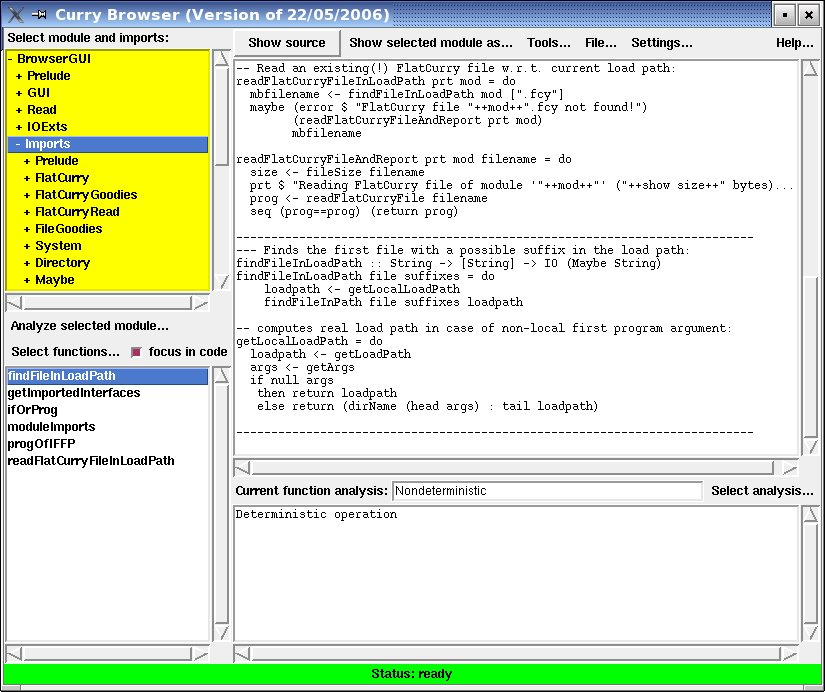
\includegraphics[scale=0.7]{currybrowser.jpg}
\end{center}
\caption{Snapshot of the main window of CurryBrowser\label{fig-currybrowser}}
\end{figure}
%
To get an impression of the use of \cb, Figure~\ref{fig-currybrowser}
shows a snapshot of its use on a particular application
(here: the implementation of \cb).
The upper list box in the left column shows the modules and their imports
in order to browse through the modules of an application.
Similarly to directory browsers, the list of imported modules of a module
can be opened or closed by clicking.
After selecting a module in the list of modules, its source code,
interface, or various other formats of the module can be shown
in the main (right) text area. For instance, one can show
pretty-printed versions of the intermediate flat programs (see below)
in order to see how local function definitions are translated by lambda lifting
\cite{Johnsson85}
or pattern matching is translated into case expressions \cite{Hanus97POPL,Wadler87}.
Since Curry is a language with parametric polymorphism and type inference,
programmers often omit the type signatures when defining functions.
Therefore, one can also view (and store) the selected module as source code where
missing type signatures are added.

Below the list box for selecting modules, there is a menu
(``Analyze selected module'') to analyze all functions
of the currently selected module at once. This is useful
to spot some functions of a module that could be problematic
in some application contexts, like functions that are impure (i.e., the result
depends on the evaluation time) or partially defined (i.e.,
not evaluable on all ground terms).
If such an analysis is selected,
the names of all functions are shown in the
lower list box of the left column (the ``function list'')
with prefixes indicating the properties of the individual functions.

The function list box can be also filled with functions
via the menu ``Select functions''. For instance, all functions
or only the exported functions defined in the currently selected
module can be shown there, or all functions from different modules
that are directly or indirectly called from
a currently selected function.
This list box is central to focus on a function in the
source code of some module or to analyze some function,
i.e., showing their properties. In order to focus on a function,
it is sufficient to check the ``focus on code'' button.
To analyze an individually selected function, one can
select an analysis from the list of available program analyses
(through the menu ``Select analysis'').
In this case, the analysis results are either shown
in the text box below the main text area
or visualized by separate tools, e.g., by a graph drawing tool for
visualizing call graphs.
Some analyses are local, i.e., they need only to consider the local definition
of this function (e.g., ``Calls directly,'' ``Overlapping rules,''
``Pattern completeness''),
where other analyses are global, i.e.,
they consider the definitions of all functions directly or indirectly called
by this function (e.g., ``Depends on,'' ``Solution complete,''
``Set-valued'').
%
Finally, there are a few additional tools integrated into \cb,
for instance, to visualize the import relation between all modules
as a dependency graph. These tools are available through the ``Tools'' menu.

More details about the use of \cb and all built-in analyses
are available through the ``Help'' menu of \cb.


\newpage

\section{CurryTest: A Tool for Testing Curry Programs}
\label{sec-currytest}

CurryTest\index{CurryTest}\index{testing programs}\index{program!testing}
is a simple tool in the PAKCS distribution to write
and run repeatable tests. CurryTest simplifies the task
of writing test cases for a module and executing them.
The tool is easy to use. Assume one has implemented a module \code{MyMod}
and wants to write some test cases to test its functionality,
making regression tests in future versions, etc.
For this purpose, there is a system library \code{Assertion}
(Section~\ref{Library:Assertion}) which
contains the necessary definitions for writing tests.
In particular, it exports an abstract polymorphic type \ccode{Assertion a}
together with the following operations:
\startprog
assertTrue      :: String -> Bool -> Assertion ()
assertEqual     :: String -> a -> a -> Assertion a
assertValues    :: String -> a -> [a] -> Assertion a
assertSolutions :: String -> (a->Success) -> [a] -> Assertion a
assertIO        :: String -> IO a -> a -> Assertion a
assertEqualIO   :: String -> IO a -> IO a -> Assertion a
\stopprog
The expression \ccode{assertTrue $s$ $b$}
is an assertion (named $s$) that the expression $b$ has the value \code{True}.
Similarly, the expression \ccode{assertEqual $s$ $e_1$ $e_2$}
asserts that the expressions $e_1$ and $e_2$
must be equal (i.e., \code{$e_1$==$e_2$} must hold),
the expression \ccode{assertValues $s$ $e$ $vs$} asserts
that $vs$ is the multiset of all values of $e$,
and the expression \ccode{assertSolutions $s$ $c$ $vs$} asserts
that the constraint abstraction $c$ has the multiset of solutions $vs$.
Furthermore, the expression \ccode{assertIO $s$ $a$ $v$}
asserts that the I/O action $a$ yields the value $v$ whenever it is
executed, and
the expression \ccode{assertEqualIO $s$ $a_1$ $a_2$}
asserts that the I/O actions $a_1$ and $a_2$ yields equal values.
The name $s$ provided as a first argument in each assertion
is used in the protocol produced by the test tool.

One can define a test program by importing the module
to be tested together with the module \code{Assertion} and defining
top-level functions of type \code{Assertion} in this module
(which must also be exported).
As an example, consider the following program
that can be used to test some list processing functions:
\startprog
\medskip
import List
import Assertion
\medskip
test1 = assertEqual     "++"     ([1,2]++[3,4]) [1,2,3,4]
\medskip
test2 = assertTrue      "all"    (all (<5) [1,2,3,4])
\medskip
test3 = assertSolutions "prefix" (\labs{}x -> let y free in  x\,++\,y =:= [1,2])
                                 [[],[1],[1,2]]
\medskip
\stopprog
For instance, \code{test1} asserts that the result of evaluating the
expression \code{([1,2]++[3,4])} is equal to \code{[1,2,3,4]}.

We can execute a test suite by the command\pindex{currytest}
\startprog
currytest testList
\stopprog
(\code{currytest} is a program stored in \code{$pakcshome$/bin}
where $pakcshome$ is the installation directory of PAKCS;
see Section~\ref{sec-general}).
In our example, \ccode{testList.curry} is the program containing the
definition of all assertions. This has the effect
that all exported top-level functions
of type \code{Assertion} are tested (i.e., the corresponding
assertions are checked) and the results
(\ccode{OK} or failure) are reported together with the name of each assertion.
%If failures occur, the complete test results are also
%written into a file named \ccode{testList.testlog}.''
For our example above, we obtain the following successful protocol:
\startprog
============================================================
Testing module "testList"...
OK: ++
OK: all
OK: prefix
All tests successfully passed.
============================================================
\stopprog
There is also a graphical interface that summarizes the results
more nicely.\footnote{Due to a bug in older versions of SICStus-Prolog,
it works only with SICStus-Prolog version 3.8.5 (or newer).}
In order to start this interface, one has to add the parameter
\ccode{--window} (or \ccode{-w}), e.g., executing a test suite by
\startprog
currytest --window testList
\stopprog
or
\startprog
currytest -w testList
\stopprog
A snapshot of the interface is shown in Figure~\ref{fig-currytest}.

\begin{figure}%[t]
\begin{center}
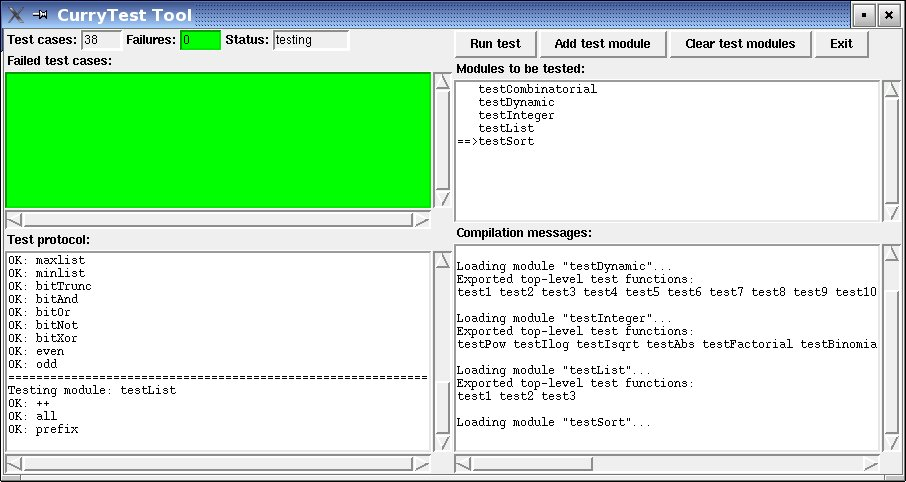
\includegraphics[scale=0.7]{currytest.jpg}
\end{center}
\caption{Snapshot of CurryTest's graphical interface\label{fig-currytest}}
\end{figure}


\newpage

\section{ERD2Curry: A Tool to Generate Programs from ER Specifications}
\label{sec-erd2curry}

ERD2Curry\index{ERD2Curry}\index{database programming}
is a tool to generate Curry code to access and manipulate data
persistently stored from
entity relationship diagrams.\index{entity relationship diagrams}
The idea of this tool is described in detail in
\cite{BrasselHanusMueller08PADL}.
Thus, we describe only the basic steps to use this tool
in the following.

If one creates an entity relationship diagram (ERD)
with the Umbrello UML Modeller, one has to store its
XML description in XMI format (as offered by Umbrello)
in a file, e.g., \ccode{myerd.xmi}.
This description can be compiled into a Curry program by the
command\pindex{erd2curry}
\startprog
erd2curry myerd.xmi
\stopprog
(\code{erd2curry} is a program stored in \code{$pakcshome$/bin}
where $pakcshome$ is the installation directory of PAKCS;
see Section~\ref{sec-general}).
If \code{MyData} is the name of the ERD, the Curry program file
\ccode{MyData.curry} is generated containing all the necessary
database access code as described in \cite{BrasselHanusMueller08PADL}.

If one does not want to use the Umbrello UML Modeller,
one can also create a textual description of the ERD
as a Curry term of type \code{ERD}
(w.r.t.\ the type definition given in module
\code{$pakcshome$/tools/erd2curry/ERD.curry})
and store it in some file, e.g., \ccode{myerd.term}.
This description can be compiled into a Curry program by the
command\pindex{erd2curry}
\startprog
erd2curry -t myerd.term
\stopprog
%
There is also the possibility to visualize an ERD term
as a graph with the graph visualization program \code{dotty}
(for this purpose, it might be necessary to adapt the definition
of the operation \code{dotCmd} in
\code{$pakcshome$/tools/erd2curry/ERD2Graph.curry}
according to your local environment).
This can be done by the command
\startprog
erd2curry -v myerd.term
\stopprog

\paragraph{Inclusion in the Curry application:}
To compile the generated database code, either
include the directory \code{$pakcshome$/tools/erd2curry}
into your Curry load path
(e.g., by setting  the environment variable
\ccode{CURRYPATH}\pindex{CURRYPATH}, see also Section~\ref{sec-modules})
or copy the file
\code{$pakcshome$/tools/erd2curry/ERDGeneric.curry}
into the directory of the generated database code.


\newpage

\section{UI: Declarative Programming of User Interfaces}
\label{sec-ui}

The PAKCS distribution contains a collection of libraries
to implement graphical user interfaces\index{user interface}
as well as web-based user interfaces
from declarative descriptions.
Exploiting these libraries, it is possible
to define the structure and functionality of a user interface
independent from the concrete technology.
Thus, a graphical user interface or a web-based user interface
can be generated from the same description by simply changing
the imported libraries.
This programming technique is described in detail in
\cite{HanusKluss09PADL}.

The libraries implementing these user interfaces are contained
in the directory
\startprog
$pakcshome$/tools/ui
\stopprog
Thus, in order to compile programs containing such user interface
specifications, one has to
include the directory \code{$pakcshome$/tools/ui}
into the Curry load path
(e.g., by setting  the environment variable
\ccode{CURRYPATH}\pindex{CURRYPATH}, see also Section~\ref{sec-modules}).
The directory
\startprog
$pakcshome$/tools/ui/examples
\stopprog
contains a few examples for such user interface specifications.


\newpage

\section{Preprocessing FlatCurry Files}
\label{sec-pakcspp}

The current parser allows to apply transformations on the intermediate
FlatCurry files after they are generated from the
corresponding Curry source file.
Currently, only the FlatCurry file corresponding to the main module
can be transformed.

A transformation can be specified as follows:
\begin{enumerate}
\item {\bf Options to \code{pakcs/bin/parsecurry}:}
\begin{description}
\item[\fbox{\code{--fpopt}}]\pindex{-fpopt}
Apply functional pattern optimization
(see \code{pakcs/tools/optimize/NonStrictOpt.curry} for details).

\item[\fbox{\code{--compact}}]\pindex{--compact}
Apply code compactification after parsing, i.e., transform the main
module and all its imported into one module and delete all
non-accessible functions.

\item[\fbox{\code{--compactexport}}]
Similar to \code{--compact} but delete all functions that are not accessible
from the exported functions of the main module.

\item[\fbox{\code{--compactmain:f}}]
Similar to \code{--compact} but delete all functions that are not accessible
from the function \ccode{f} of the main module.

\item[\fbox{\code{--fcypp cmd}}]\pindex{--fcypp}
Apply command \code{cmd} to the main module after parsing. This is useful to
integrate your own transformation into the compilation process.
Note that the command \ccode{cmd prog} should perform a transformation
on the FlatCurry file \code{prog.fcy}, i.e., it replaces the FlatCurry
file by a new one.
\end{description}

\item {\bf Setting the environment variable \code{FCYPP}:}\pindex{FCYPP}\\
For instance, setting \code{FCYPP} by
\startprog
export FCYPP="--fpopt"
\stopprog
will apply the functional pattern optimization if programs are compiled
and loaded in the PAKCS programming environment.


\item {\bf Putting options into the source code:}\pindex{PAKCS_OPTION_FCYPP}\\
If the source code contains a line with a comment of the form (the comment
must start at the beginning of the line)
\startprog
\{-\# PAKCS_OPTION_FCYPP <options> \#-\}
\stopprog
then the transformations specified by \code{<options>} are applied after
translating the source code into FlatCurry code. For instance,
the functional pattern optimization can be set by the comment
\startprog
\{-\# PAKCS_OPTION_FCYPP --fpopt \#-\}
\stopprog
in the source code. Note that this comment must be in a single line 
of the source program. If there are multiple lines containing such comments,
only the first one will be considered.
\end{enumerate}
\paragraph{Multiple options:}
Note that an arbitrary number of transformations can be specified
by the methods described above.
If several specifications for preprocessing FlatCurry files are used,
they are executed in the following order:
\begin{enumerate}
\item all transformations specified by the environemnt variable
\code{FCYPP} (from left to right)
\item all transformations specified as command line options of parsecurry
   (from left to right)
\item all transformations specified by a comment line in the source code
   (from left to right)
\end{enumerate}


\newpage

\section{Technical Problems}

Due to the fact that Curry is intended to implement
distributed systems (see Appendix~\ref{sec-ports}),
it might be possible that some technical problems
arise due to the use of sockets for implementing these
features. Therefore, this section gives some information
about the technical requirements of PAKCS and how to solve
problems due to these requirements.

There is one fixed port that is used by the implementation of PAKCS:
\begin{description}
\item[Port 8766:] This port is used by the
{\bf Curry Port Name Server} (CPNS) to implement symbolic names for
ports in Curry (see Appendix~\ref{sec-ports}).
If some other process uses this port on the machine,
the distribution facilities defined in the module \code{Ports}
(see Appendix~\ref{sec-ports}) cannot be used.
\end{description}
If these features do not work, you can try to find out
whether this port is in use by the shell command
\ccode{netstat -a | fgrep 8766} (or similar).

The CPNS is implemented as a demon listening on its port 8766
in order to serve requests about registering a new symbolic
name for a Curry port or asking the physical port number
of a Curry port. The demon will be automatically started for
the first time on a machine when a user compiles a program
using Curry ports. It can also be manually started and terminated by the
scripts \code{$pakcshome$/cpns/start} and
\code{$pakcshome$/cpns/stop}.
If the demon is already running, the command \code{$pakcshome$/cpns/start}
does nothing (so it can be always executed
before invoking a Curry program using ports).

If you detect any further technical problem,
please write to
\begin{center}
\code{mh@informatik.uni-kiel.de}
\end{center}

\newpage

\addcontentsline{toc}{section}{Bibliography}
\bibliography{manual}
\bibliographystyle{plain}

\newpage
\appendix

\section{Libraries of the PAKCS Distribution}
\label{sec:libraries}

{\setlength{\parindent}{0.0cm}

The PAKCS compiler system provides an extensive collection
of libraries for application programming.
The libraries for arithmetic constraints over real numbers,
finite domain constraints,
ports for concurrent and distributed programming, and
meta-programming by representing Curry programs in Curry
are described in the following subsection in more detail.
The complete set of libraries with all exported types and functions
are described in the further subsections.
For a more detailed online documentation of all libraries of PAKCS,
see \url{http://www.informatik.uni-kiel.de/~pakcs/lib/index.html}.

\subsection{Constraints, Ports, Meta-Programming}

\subsubsection{Arithmetic Constraints}

The primitive entities for the use of arithmetic constraints
are defined in the system module \code{CLPR}
(cf.\ Section~\ref{sec-modules}), i.e., in order to use them,
the program must contain the import declaration
\startprog
import CLPR
\stopprog
Floating point arithmetic is supported in PAKCS
via arithmetic constraints, i.e., the equational constraint
\ccode{2.3 +.~x =:= 5.5} is solved by binding \code{x} to \code{3.2}
(rather than suspending the evaluation of the addition,
as in corresponding constraints on integers like
\ccode{3+x=:=5}). All operations related to
floating point numbers are suffixed by \ccode{.}.
The following functions and constraints on floating point
numbers are supported in PAKCS:
\begin{description}
\item[\code{(+.)   :: Float -> Float -> Float}]~\\
Addition on floating point numbers.
\item[\code{(-.)   :: Float -> Float -> Float}]~\\
Subtraction on floating point numbers.
\item[\code{(*.)   :: Float -> Float -> Float}]~\\
Multiplication on floating point numbers.
\item[\code{(/.)   :: Float -> Float -> Float}]~\\
Division on floating point numbers.
\item[\code{(<.)   :: Float -> Float -> Success}]~\\
Comparing two floating point numbers with the ``less than'' relation.
\item[\code{(>.)   :: Float -> Float -> Success}]~\\
Comparing two floating point numbers with the ``greater than'' relation.
\item[\code{(<=.)  :: Float -> Float -> Success}]~\\
Comparing two floating point numbers with the ``less than or equal'' relation.
\item[\code{(>=.)  :: Float -> Float -> Success}]~\\
Comparing two floating point numbers with the ``greater than or equal''
relation.
\item[\code{i2f    :: Int -> Float}]~\\
Converting an integer number into a floating point number.
\end{description}
As an example, consider a constraint \code{mortgage}
which relates the principal \code{p},
the lifetime of the mortgage in months \code{t},
the monthly interest rate \code{ir},
the monthly repayment \code{r},
and the outstanding balance at the end of the lifetime \code{b}.
The financial calculations
can be defined by the following two rules in Curry (the second rule
describes the repeated accumulation of the interest):
\startprog
~
import CLPR
~
mortgage p t ir r b | t >. 0.0 \& t <=. 1.0  --lifetime not more than 1 month?
                    =  b =:= p *. (1.0 +. t *. ir) -. t*.r \vspace{1ex}
mortgage p t ir r b | t >. 1.0               --lifetime more than 1 month?
                    =  mortgage (p *. (1.0+.ir)-.r) (t-.1.0) ir r b
~
\stopprog
Then we can calculate the monthly payment for paying back
a loan of \$100,000 in 15 years with a monthly interest rate of 1\%
by solving the goal
\startprog
mortgage 100000.0 180.0 0.01 r 0.0
\stopprog
which yields the solution \code{r=1200.17}.

Note that only linear arithmetic equalities or inequalities
are solved by the constraint solver. Non-linear constraints
like \ccode{x *.~x =:= 4.0} are suspended until they become
linear.


\subsubsection{Finite Domain Constraints}

Finite domain constraints are constraints where all variables
can only take a finite number of possible values.
For simplicity, the domain of finite domain variables are
identified with a subset of the integers, i.e., the type
of a finite domain variable is \code{Int}. The arithmetic
operations related to finite domain variables are suffixed by \ccode{\#}.
The following functions and constraints for finite domain constraint solving
are currently supported in PAKCS:\footnote{Note that
this library is based on the corresponding library of SICStus-Prolog
but does not implement the complete functionality of the SICStus-Prolog library.
However, using the PAKCS interface for external functions (see
Appendix~\ref{sec-external-functions}), it is relatively
easy to provide the complete functionality.}

\begin{description}
\item[\code{domain :: [Int] -> Int -> Int -> Success}]~\\
The constraint \ccode{domain [$x_1,\ldots,x_n$] $l$ $u$}
is satisfied if the domain of all variables $x_i$ is the interval $[l,u]$.
\item[\code{(+\#)   :: Int -> Int -> Int}]~\\
Addition on finite domain values.
\item[\code{(-\#)   :: Int -> Int -> Int}]~\\
Subtraction on finite domain values.
\item[\code{(*\#)   :: Int -> Int -> Int}]~\\
Multiplication on finite domain values.
\item[\code{(=\#)   :: Int -> Int -> Success}]~\\
Equality of finite domain values.
\item[\code{(/=\#)  :: Int -> Int -> Success}]~\\
Disequality of finite domain values.
\item[\code{(<\#)   :: Int -> Int -> Success}]~\\
``less than'' relation on finite domain values.
\item[\code{(<=\#)  :: Int -> Int -> Success}]~\\
``less than or equal'' relation on finite domain values.
\item[\code{(>\#)   :: Int -> Int -> Success}]~\\
``greater than'' relation on finite domain values.
\item[\code{(>=\#)  :: Int -> Int -> Success}]~\\
``greater than or equal'' relation on finite domain values.
\item[\code{sum :: [Int] -> (Int -> Int -> Success) -> Int -> Success}]~\\
The constraint \ccode{sum [$x_1,\ldots,x_n$] $op$ $x$}
is satisfied if all $x_1+\cdots + x_n \mathrel{op} x$ is satisfied,
where $op$ is one of the above finite domain constraint relations
(e.g., \ccode{=\#}).
\item[\code{scalar_product :: [Int] -> [Int] -> (Int -> Int -> Success) -> Int -> Success}]~\\
The constraint \ccode{scalar_product [$c_1,\ldots,c_n$] [$x_1,\ldots,x_n$] $op$ $x$}
is satisfied if all $c_1 x_1+\cdots + c_n x_n \mathrel{op} x$ is satisfied,
where $op$ is one of the above finite domain constraint relations.
\item[\code{count :: Int -> [Int] -> (Int -> Int -> Success) -> Int -> Success}]~\\
The constraint \ccode{count $k$ [$x_1,\ldots,x_n$] $op$ $x$}
is satisfied if all $k \mathrel{op} x$ is satisfied,
where $n$ is the number of the $x_i$ that are equal to $k$ and
$op$ is one of the above finite domain constraint relations.
\item[\code{all_different :: [Int] -> Success}]~\\
The constraint \ccode{all_different [$x_1,\ldots,x_n$]}
is satisfied if all $x_i$ have pairwise different values.
\item[\code{labeling :: [LabelingOption] -> [Int] -> Success}]~\\
The constraint \ccode{labeling $os$ [$x_1,\ldots,x_n$]}
non-deterministically instantiates all $x_i$ to the values
of their domain according to the options $os$ (see the module documentation
for further details about these options).
\end{description}
These entities are defined in the system module \code{CLPFD}
(cf.\ Section~\ref{sec-modules}), i.e., in order to use it,
the program must contain the import declaration
\startprog
import CLPFD
\stopprog
As an example, consider the classical \ccode{send+more=money} problem
where each letter must be replaced by a different digit such that this
equation is valid and there are no leading zeros.
The usual way to solve finite domain constraint problems
is to specify the domain of the involved variables followed
by a specification of the constraints and the labeling
of the constraint variables in order to start the search for solutions.
Thus, the \ccode{send+more=money} problem can be solved as follows:
\startprog
~
import CLPFD
~
smm l =
        l =:= [s,e,n,d,m,o,r,y] \&
        domain l 0 9 \&
        s >\# 0 \&
        m >\# 0 \&
        all_different l  \&
                         1000 *\# s +\# 100 *\# e +\# 10 *\# n +\# d
        +\#               1000 *\# m +\# 100 *\# o +\# 10 *\# r +\# e
        =\# 10000 *\# m +\# 1000 *\# o +\# 100 *\# n +\# 10 *\# e +\# y \&
        labeling [FirstFail] l
        where s,e,n,d,m,o,r,y free
~
\stopprog
Then we can solve this problem by evaluating the goal
\ccode{smm [s,e,n,d,m,o,r,y]} which yields the unique solution
\code{\{s=9,e=5,n=6,d=7,m=1,o=0,r=8,y=2\}}.


\subsubsection{Ports: Distributed Programming in Curry}
\label{sec-ports}

To support the development of concurrent and distributed applications,
PAKCS supports internal and external ports\index{ports} as
described in \cite{Hanus99PPDP}.
Since \cite{Hanus99PPDP} contains a detailed description of this
concept together with various programming examples, we only summarize here
the functions and constraints supported for ports in PAKCS.

The basic datatypes, functions, and constraints for ports
are defined in the system module \code{Ports}
(cf.\ Section~\ref{sec-modules}), i.e., in order to use ports,
the program must contain the import declaration
\startprog
import Ports
\stopprog
This declaration includes the following entities in the program:
\begin{description}
\item[\code{Port a}\pindex{Port}]~\\
This is the datatype of a port to which one can send messages of type \code{a}.

\item[\code{openPort :: Port a -> [a] -> Success}]~\\
The constraint \ccode{openPort p s}\pindex{openPort}
establishes a new \emph{internal port}
\code{p} with an associated message stream \code{s}. \code{p} and \code{s} must be
unbound variables,
otherwise the constraint fails (and causes a runtime error).

\item[\code{send :: a -> Port a -> Success}]~\\
The constraint \ccode{send m p}\pindex{send}
is satisfied if \code{p} is constrained
to contain the message \code{m}, i.e., \code{m} will be sent to the port
\code{p} so that it appears in the corresponding stream.

\item[\code{doSend :: a -> Port a -> IO ()}]~\\
The I/O action \ccode{doSend m p}\pindex{doSend} solves the constraint
\ccode{send m p} and returns nothing.

\item[\code{openNamedPort :: String -> IO [a]}]~\\
The I/O action \ccode{openNamedPort n}\pindex{openNamedPort}
opens a new \emph{external port} with
symbolic name \code{n} and returns the associated stream of messages.

\item[\code{connectPort :: String -> IO (Port a)}]~\\
The I/O action \ccode{connectPort n}\pindex{connectPort}
returns a port with symbolic name
\code{n} (i.e., \code{n} must have the form ``\emph{portname@machine})
to which one can send messages by the \code{send} constraint.
Currently, no dynamic type checking is done for external ports,
i.e., sending messages of the wrong type to a port might lead to
a failure of the receiver.
\end{description}

\paragraph{Restrictions:}
Every expression, possibly containing logical variables, can be sent to
a port. However, as discussed in \cite{Hanus99PPDP},
port communication is strict, i.e., the expression is
evaluated to normal form before sending it by the
constraint \code{send}. Furthermore, if messages containing
logical variables are sent to \emph{external ports},
the behavior is as follows:
\begin{enumerate}
\item The sender waits until all logical variables in the message
have been bound by the receiver.
\item The binding of a logical variable received by a process
is sent back to the sender of this logical variable only if
it is bound to a \emph{ground} term, i.e., as long as the binding contains
logical variables, the sender is not informed about the binding
and, therefore, the sender waits.
\end{enumerate}

\paragraph{External ports on local machines:}
The implementation of external ports assumes that the
host machine running the application is connected to the Internet
(i.e., it uses the standard IP address of the host machine
for message sending). If this is not the case and the application
should be tested by using external ports only on the local host
without a connection to the Internet,
the environment variable \ccode{PAKCS_LOCALHOST}\pindex{PAKCS_LOCALHOST}
must be set to \ccode{yes}
\emph{before PAKCS system is started}.
In this case, the IP address \code{127.0.0.1} and the hostname
\ccode{localhost} are used for identifying the local machine.

\paragraph{Selection of Unix sockets for external ports:}
The implementation of ports uses sockets to communicate
messages sent to external ports.
Thus, if a Curry program uses the
I/O action \code{openNamedPort}\pindex{openNamedPort}
to establish an externally visible server,
PAKCS selects a Unix socket for the port communication.
Usually, a free socket is selected by the operating system.
If the socket number should be fixed in an application (e.g.,
because of the use of firewalls\index{firewall} that allow only
communication over particular sockets), then one
can set the environment variable \ccode{PAKCS_SOCKET}\pindex{PAKCS_SOCKET}
to a distinguished socket number before the PAKCS system is started.
This has the effect that PAKCS uses only this socket
number for communication (even for several external ports
used in the same application program).

\paragraph{Debugging:}
To debug distributed systems,
it is sometimes helpful to see all messages sent to external ports.
This is supported by the environment variable
\ccode{PAKCS_TRACEPORTS}.\pindex{PAKCS_TRACEPORTS}
If this variable is set to \ccode{yes}
\emph{before the PAKCS system is started}, then all
connections to external ports and all
messages sent and received on external ports are
printed on the standard error stream.


\subsubsection{AbstractCurry and FlatCurry: Meta-Programming in Curry}
\label{sec-flatcurry}

\index{AbstractCurry}
\index{FlatCurry}
To support meta-programming, i.e., the manipulation of Curry programs
in Curry, there are system modules \code{FlatCurry} and \code{AbstractCurry}
(stored in the directory \ccode{$pakcshome$/lib/meta})
which define datatypes for the representation
of Curry programs.
\code{AbstractCurry} is a more direct representation of a Curry program,
whereas \code{FlatCurry} is a simplified representation
where local function definitions are replaced by global definitions
(i.e., lambda lifting has been performed) and pattern matching
is translated into explicit case/or expressions.
Thus, \code{FlatCurry} can be used for more back-end oriented
program manipulations (or, for writing new back ends for Curry),
whereas \code{AbstractCurry} is intended for manipulations of
programs that are more oriented towards the source program.

Both modules contain predefined I/O actions to read programs
in the \code{AbstractCurry} (\code{readCurry}\pindex{readCurry})
or \code{FlatCurry}
(\code{readFlatCurry}\pindex{readFlatCurry}) format.
These actions parse the corresponding source program and return
a data term representing this program (according to the definitions
in the modules \code{AbstractCurry} and \code{FlatCurry}).

Since all datatypes are explained in detail in these modules,
we refer to the online documentation\footnote{%
\url{http://www.informatik.uni-kiel.de/~pakcs/lib/CDOC/FlatCurry.html} and
\url{http://www.informatik.uni-kiel.de/~pakcs/lib/CDOC/AbstractCurry.html}}
of these modules.

As an example, consider a program file \ccode{test.curry}
containing the following two lines:
\startprog
rev []     = []
rev (x:xs) = (rev xs) ++ [x]
\stopprog
Then the I/O action \code{(FlatCurry.readFlatCurry "test")} returns the
following term:
\startprog
 (Prog "test"
  ["Prelude"]
  []
  [Func ("test","rev") 1 Public
        (FuncType (TCons ("Prelude","[]") [(TVar 0)])
                  (TCons ("Prelude","[]") [(TVar 0)]))
        (Rule [0]
           (Case Flex (Var 0)
              [Branch (Pattern ("Prelude","[]") [])
                  (Comb ConsCall ("Prelude","[]") []),
               Branch (Pattern ("Prelude",":") [1,2])
                  (Comb FuncCall ("Prelude","++")
                        [Comb FuncCall ("test","rev") [Var 2],
                         Comb ConsCall ("Prelude",":")
                              [Var 1,Comb ConsCall ("Prelude","[]") []]
                        ])
              ]))]
  []
 )
\stopprog


%%%%%%%%%%%%%%%%%%%%%%%%%%%%%%%%%%%%%%%%%%%%%%%%%%%%%%%%%%%%%%%%%%%%%%%%%
% Definitions in order to LaTeX documents generated by "currydoc --tex"
%%%%%%%%%%%%%%%%%%%%%%%%%%%%%%%%%%%%%%%%%%%%%%%%%%%%%%%%%%%%%%%%%%%%%%%%%

\newcommand{\currymodule}[1]{\subsubsection{Library #1}\label{Library:#1}}
\newcommand{\currytypesstart}{\subsubsection*{Exported types:}}
\newcommand{\currytypesstop}{}
\newcommand{\currytypesynstart}[2]{{\tt type #2}\pindex{#1} \begin{quote}}
\newcommand{\currytypesynstop}{\end{quote}}
\newcommand{\currydatastart}[1]{{\tt data #1}\pindex{#1} \begin{quote}}
\newcommand{\currydatacons}{\end{quote}%
\begin{itemize}\item[] \hspace{-4ex}\emph{Exported constructors:}}
\newcommand{\currydatastop}{\end{itemize}}
\newcommand{\curryconsstart}[2]{\item {\tt #1~::~#2}\par}
\newcommand{\curryfuncstart}{\subsubsection*{Exported functions:}}
\newcommand{\curryfuncstop}{}
\newcommand{\curryfunctionstart}[2]{#2\pindex{#1}\begin{quote}}
\newcommand{\curryfunctionstop}{\end{quote}}
\newcommand{\curryfuncsig}[2]{{\tt #1~::~#2}}


\subsection{General Libraries}

\input{lib/AllSolutions}
\input{lib/Assertion}
\input{lib/Char}
\input{lib/CLPFD}
\input{lib/CLPR}
\input{lib/CLPB}
\input{lib/Combinatorial}
\input{lib/Constraint}
\input{lib/CSV}
\input{lib/Database}
\input{lib/DaVinci}
\input{lib/Directory}
\input{lib/Dynamic}
\input{lib/FileGoodies}
\input{lib/Float}
\input{lib/Global}
\input{lib/GlobalVariable}
\input{lib/GUI}
\input{lib/Integer}
\input{lib/IO}
\input{lib/IOExts}
\input{lib/JavaScript}
\input{lib/KeyDatabase}
\input{lib/KeyDatabaseSQLite}
\input{lib/KeyDB}
\input{lib/List}
\input{lib/Maybe}
\input{lib/NamedSocket}
\input{lib/Parser}
\input{lib/Ports}
\input{lib/Pretty}
\input{lib/Profile}
\input{lib/PropertyFile}
\input{lib/Read}
\input{lib/ReadNumeric}
\input{lib/ReadShowTerm}
\input{lib/SetFunctions}
\input{lib/Socket}
\input{lib/System}
\input{lib/Time}
%\input{lib/Tk}
\input{lib/Unsafe}


\subsection{Data Structures and Algorithms}

\input{lib/Array}
\input{lib/Dequeue}
\input{lib/FiniteMap}
\input{lib/GraphInductive}
\input{lib/Random}
\input{lib/RedBlackTree}
\input{lib/SetRBT}
\input{lib/Sort}
\input{lib/TableRBT}
\input{lib/Traversal}

\subsection{Libraries for Web Applications}

\input{lib/CategorizedHtmlList}
\input{lib/HTML}
\input{lib/HtmlParser}
\input{lib/Mail}
\input{lib/Markdown}
\input{lib/WUI}
\input{lib/URL}
\input{lib/XML}
\input{lib/XmlConv}

\subsection{Libraries for Meta-Programming}

\input{lib/AbstractCurry}
\input{lib/AbstractCurryPrinter}
\input{lib/CompactFlatCurry}
\input{lib/CurryStringClassifier}
\input{lib/FlatCurry}
\input{lib/FlatCurryGoodies}
\input{lib/FlatCurryRead}
\input{lib/FlatCurryShow}
\input{lib/FlatCurryTools}
\input{lib/FlatCurryXML}
\input{lib/FlexRigid}
\input{lib/PrettyAbstract}

} % end setlength parindent

\newpage

\input{markdown_syntax}

\newpage

\begin{figure}%[t]
\begin{center}
 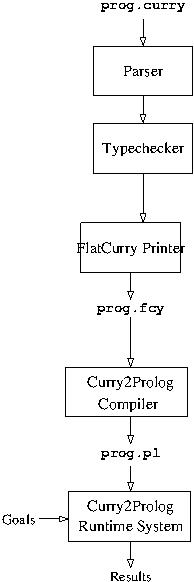
\includegraphics[scale=0.85]{pakcs_overview.jpg}
\end{center}\vspace{-5ex}
\caption{Overview of PAKCS\label{fig-pakcs}}
\end{figure}

\section{Overview of the PAKCS Distribution}

A schematic overview of the various components contained in
the distribution of PAKCS and the
translation process of programs inside PAKCS is shown in
Figure~\ref{fig-pakcs} on page~\pageref{fig-pakcs}.
In this figure, boxes denote different components of PAKCS
and names in boldface denote files containing
various intermediate representations during the translation
process (see Section~\ref{sec-auxfiles} below).
The PAKCS distribution contains a front end for reading (parsing and
type checking) Curry programs that can be also used by
other Curry implementations.
The back end (formerly known as ``Curry2Prolog''\index{Curry2Prolog})
compiles Curry programs into Prolog programs.
It also support constraint solvers for
arithmetic constraints over real numbers and finite domain constraints,
and further libraries for GUI programming, meta-programming etc.
Currently, it does not implement encapsulated search in full generality
(only a strict version of \code{findall} is supported),
and concurrent threads are not executed in a fair manner.


\newpage

\section{Auxiliary Files}
\label{sec-auxfiles}

During the translation and execution of a Curry program with PAKCS,
various intermediate representations of the source program are created
and stored in different files which are shortly explained in this section.
If you use the PAKCS, it is not necessary to know about
these auxiliary files because they are automatically generated
and updated. You should only remember the command for deleting
all auxiliary files (\ccode{cleancurry}, see Section~\ref{sec-general})
to clean up your directories.

The various components of PAKCS create
the following auxiliary files.
\begin{description}
\item[\code{prog.fcy}:] This file contains the Curry program
in the so-called ``FlatCurry'' representation where all functions are global
(i.e., lambda lifting has been performed) and pattern matching
is translated into explicit case/or expressions
(compare Appendix~\ref{sec-flatcurry}).
This representation might be useful for other back ends and
compilers for Curry and is the basis doing meta-programming in Curry.
This file is implicitly
generated when a program is read by PAKCS.
It can be also explicitly generated by the command\pindex{parsecurry}
\startprog
parsecurry --flat prog
\stopprog
The FlatCurry representation of a Curry program is usually
generated by the front-end after parsing, type checking and eliminating
local declarations.
If $dir$ is the directory where the Curry program is stored,
the corresponding FlatCurry program is stored in the directory
\ccode{$dir$/.curry}.

\item[\code{prog.fint}:] This file contains the interface
of the program in the so-called ``FlatCurry'' representation,
i.e., it is similar to \code{prog.fcy} but contains only exported
entities and the bodies of all functions omitted (i.e., ``external'').
This representation is useful for providing a fast access
to module interfaces.
This file is implicitly generated by the command\pindex{parsecurry}
\startprog
parsecurry --flat prog
\stopprog
and stored in the same directory as \code{prog.fcy}.

\item[\code{prog.pl}:] This file contains a Prolog program
as the result of translating the Curry program with PAKCS.
If $dir$ is the directory where the Curry program is stored,
the corresponding Prolog program is stored in the directory
\ccode{$dir$/.curry/.pakcs}.

\item[\code{prog.po}:] This file contains the Prolog program
\code{prog.pl} in an intermediate format for faster loading.
This file is stored in the same directory as \code{prog.pl}.

\item[\code{prog.state}:] This file contains the saved state
after compiling and saving a program with PAKCS
(see Section~\ref{sec-use-curry2prolog}).

\end{description}


\newpage


\section{Changing the Prelude or System Modules}

The standard prelude, which is automatically imported into each Curry program,
and all system modules containing datatypes and functions
useful for application programming
(cf.\ Appendix~\ref{sec:libraries})
are stored in the system module directory \ccode{$pakcshome$/lib}
(and its subdirectories).
If you change any of these modules,
you have to recompile the complete system by
executing \code{make} in the directory $pakcshome$.



\newpage

\section{External Functions}
\label{sec-external-functions}

\index{function!external}\index{external function}
Currently, PAKCS has no general interface to external functions.
Therefore, if a new external function should be added
to the system, this function must be declared as \code{external}
in the Curry source code
and then an implementation for this external function
must be inserted in the corresponding back end.
An external function is defined as follows in the Curry source code:
\begin{enumerate}
\item
Add a type declaration for the external function somewhere
in the body of the appropriate file (usually, the prelude
or some system module).
\item
For external functions it is not allowed to define any
rule since their semantics is determined by an external implementation.
Instead of the defining rules, you have to write
\startprog
f external
\stopprog
somewhere in the file containing the type declaration for 
the external function \code{f}.
\end{enumerate}
For instance, the addition on integers can be declared as
an external function as follows:
\startprog
(+) :: Int -> Int -> Int
(+) external
\stopprog
The further modifications to be done for an inclusion of
an external function has to be done in the back end.
A new external function is added to the back end of PAKCS
by informing the compiler about the existence of an external function
and adding an implementation of this function in the run-time
system. Therefore, the following items must be added
in the PAKCS compiler system:
\begin{enumerate}
\item
If the Curry module \code{Mod} contains external functions,
there must be a file named \code{Mod.prim_c2p} containing the
specification of these external functions. The contents of this file
is in XML format and has the following general structure:\footnote{%
\url{http://www.informatik.uni-kiel.de/~pakcs/primitives.dtd} contains a DTD
describing the exact structure of these files.}
\startprog
<primitives>
  \emph{specification of external function $f_1$}
  \ldots
  \emph{specification of external function $f_n$}
</primitives>
\stopprog
The specification of an external function $f$
with arity $n$ has the form
\startprog
<primitive name="$f$" arity="$n$">
  <library>lib</library>
  <entry>pred</entry>
</primitive>
\stopprog
where \code{lib} is the Prolog library (stored in the directory of the
Curry module or in the global directory
\code{$pakcshome$/curry2prolog/lib_src}) containing the code implementing this
function and \code{pred} is a predicate name in this library
implementing this function. Note that the function $f$ must be
declared in module \code{Mod}: either as an external function
or defined in Curry by equations. In the latter case,
the Curry definition is not translated but calls to this function
are redirected to the Prolog code specified above.

Furthermore, the list of specifications can also contain entries of the form
\startprog
<ignore name="$f$" arity="$n$" />
\stopprog
for functions $f$ with arity $n$ that are declared in module \code{Mod}
but should be ignored for code generation, e.g., since they are
never called w.r.t.\ to the current implementation of external functions.
For instance, this is useful when functions that can
be defined in Curry should be (usually more efficiently) are implemented
as external functions.

Note that the arguments are passed in their current (possibly unevaluated) form.
Thus, if the external function requires the arguments to be evaluated
in a particular form, this must be done before calling the external function.
For instance, the external function for adding two integers
requires that both arguments must be evaluated to non-variable head normal form
(which is identical to the ground constructor normal form). Therefore,
the function \ccode{+} is specified in the prelude by
\startprog
(+)   :: Int -> Int -> Int
x + y = (prim_Int_plus \$\# y) \$\# x
\medskip
prim_Int_plus :: Int -> Int -> Int
prim_Int_plus external
\stopprog
where \code{prim_Int_plus} is the actual external function implementing
the addition on integers. Consequently, the specification file
\code{Prelude.prim_c2p} has an entry of the form
\startprog
<primitive name="prim_Int_plus" arity="2">
  <library>prim_standard</library>
  <entry>prim_Int_plus</entry>
</primitive>
\stopprog
where the Prolog library \code{prim_standard.pl} contains the Prolog code
implementing this function.

\item
For most external functions, a \emph{standard interface} is
generated by the compiler so that an $n$-ary function can be
implemented by an $(n+1)$-ary predicate where the last argument must
be instantiated to the result of evaluating the function.  The
standard interface can be used if all arguments are ensured to be
fully evaluated (e.g., see definition of \code{(+)} above) and no
suspension control is necessary, i.e., it is ensured that the
external function call does not suspend for all arguments.
Otherwise, the raw interface (see below) must be used.  For
instance, the Prolog code implementing \code{prim_Int_plus}
contained in the Prolog library \code{prim_standard.pl} is as
follows (note that the arguments of \code{(+)} are passed in reverse
order to \code{prim_Int_plus} in order to ensure a left-to-right
evaluation of the original arguments by the calls to \code{(\$\#)}):
\startprog
prim_Int_plus(Y,X,R) :- R is X+Y.
\stopprog

\item
The \emph{standard interface for I/O actions}, i.e., external functions
with result type \code{IO~a}, assumes that the I/O action
is implemented as a predicate (with a possible side effect)
that instantiates the last argument to the returned value of type \ccode{a}.
For instance, the primitive predicate \code{prim_getChar}
implementing prelude I/O action \code{getChar}
can be implemented by the Prolog code
\startprog
prim_getChar(C) :- get_code(N), char_int(C,N).
\stopprog
where \code{char_int} is a predicate relating the internal
Curry representation of a character with its ASCII value.

\item
If some arguments passed to the external functions are not fully evaluated
or the external function might suspend, the implementation must follow
the structure of the PAKCS run-time system by using
the \emph{raw interface}. In this case, the name of the external entry
must be suffixed by \ccode{[raw]} in the \code{prim_c2p} file.
For instance, if we want to use the raw interface for the external function
\code{prim_Int_plus},
the specification file \code{Prelude.prim_c2p} must have an entry of the form
\startprog
<primitive name="prim_Int_plus" arity="2">
  <library>prim_standard</library>
  <entry>prim_Int_plus[raw]</entry>
</primitive>
\stopprog
In the raw interface, the actual implementation of an $n$-ary external function consists
of the definition of an $(n+3)$-ary predicate $pred$.
The first $n$ arguments are the corresponding actual arguments.
The $(n+1)$-th argument is a free variable which must be
instantiated to the result of the function call after
successful execution. The last two arguments
control the suspension behavior of the function
(see \cite{AntoyHanus00FROCOS} for more details):
The code for the predicate $pred$
should only be executed when the $(n+2)$-th argument
is not free, i.e., this predicate has always the
SICStus-Prolog block declaration
\startprog
?- block $pred$(?,\ldots,?,-,?).
\stopprog
In addition, typical external functions should suspend
until the actual arguments are instantiated. This can be ensured
by a call to \code{ensureNotFree} or \code{(\$\#)}
before calling the external function. Finally, the
last argument (which is a free variable at call time)
must be unified with the $(n+2)$-th argument
after the function call is successfully evaluated
(and does not suspend). Additionally, the actual (evaluated) arguments
must be dereferenced before they are accessed.
Thus, an implementation
of the external function for adding integers is as follows in the raw interface:
\startprog
?- block prim_Int_plus(?,?,?,-,?).
prim_Int_plus(RY,RX,Result,E0,E) :-
     deref(RX,X), deref(RY,Y), Result is X+Y, E0=E.
\stopprog
Here, \code{deref} is a predefined predicate for dereferencing the
actual argument into a constant (and \code{derefAll} for dereferencing
complex structures).
\end{enumerate}
%
The Prolog code implementing the external functions must be accessible to the run-time
system of PAKCS by putting it into the directory containing the corresponding
Curry module or into the system directory
\code{$pakcshome$/curry2prolog/lib_src}.
Then it will be automatically loaded into the run-time environment
of each compiled Curry program.

Note that arbitrary functions implemented in C or Java can be connected to
PAKCS by using the corresponding interfaces of underlying Prolog system.


\newpage
\addcontentsline{toc}{section}{Index}
\printindex


\end{document}

\clearpage
\documentclass[11pt,fleqn]{article}

\usepackage{latexsym}
\usepackage{makeidx}
\usepackage{url}
\usepackage{xspace}
\usepackage{graphicx}

\input{version}

%%% ------------------------------------------------------------------

\usepackage[colorlinks,linkcolor=blue]{hyperref}
\hypersetup{bookmarksopen=true}
\hypersetup{bookmarksopenlevel=0}
\hypersetup{pdftitle={PAKCS: The Portland Aachen Kiel Curry System}}
\hypersetup{pdfauthor={Michael Hanus}}
%\hypersetup{pdfstartview=Title}
\hypersetup{pdfstartview=FitH}
\usepackage{thumbpdf}

%%% ------------------------------------------------------------------

\setlength{\textwidth}{16.5cm}
\setlength{\textheight}{23cm}
\renewcommand{\baselinestretch}{1.1}
\setlength{\topmargin}{-1cm}
\setlength{\oddsidemargin}{0cm}
\setlength{\evensidemargin}{0cm}
\setlength{\marginparwidth}{0.0cm}
\setlength{\marginparsep}{0.0cm}

\newlength{\figurewidth}
\setlength{\figurewidth}{\textwidth}
\addtolength{\figurewidth}{-0.4cm}

% font for program texts
\renewcommand{\tt}{\usefont{OT1}{cmtt}{m}{n}\selectfont}
\newcommand{\codefont}{\tt}

% environment for typing program texts:
\makeatletter
\newenvironment{prog}{\par\vspace{0.7ex}
\setlength{\parindent}{1.0cm}
\setlength{\parskip}{-0.1ex}
\obeylines\@vobeyspaces\tt}{\vspace{0.7ex}\noindent
}
\makeatother
\newcommand{\startprog}{\begin{prog}}
\newcommand{\stopprog}{\end{prog}\noindent}

% program text in normal text
\newcommand{\code}[1]{\mbox{\codefont #1}}

% program text in normal text with apostrophs
\newcommand{\ccode}[1]{``\mbox{\codefont #1}''}

\newcommand{\pindex}[1]{\index{#1@{\tt #1}}}  % program elements in index

\newcommand{\labs}{\mbox{\tt\char92}}  % lambda abstraction in Curry
\newcommand{\todo}[1]{\fbox{\sc To do: #1}}
\newcommand{\cb}{CurryBrowser\xspace}

% allow underscores in programs:
\catcode`\_=\active
\let_=\sb
\catcode`\_=12

% produce an index:
\makeindex

\begin{document}
\sloppy

\begin{titlepage}
\pdfbookmark[1]{Title}{Title}
\begin{center}
\fbox{
\begin{minipage}[t]{\figurewidth}
\begin{center}\vspace{10ex}
{\Huge\bf PAKCS \pakcsversion}\\[4ex]
{\huge The Portland Aachen Kiel Curry System}\\[7ex]
{\huge User Manual}\\[4ex]
\pakcsversiondate\\[6ex]
\Large
Michael Hanus$^1$ [editor] \\[3ex]
{\large Additional Contributors:}\\[2ex]
Sergio Antoy$^2$ \\
Bernd Bra\ss{}el$^3$ \\
Martin Engelke$^4$ \\
Klaus H\"oppner$^5$ \\
Johannes Koj$^6$ \\
Philipp Niederau$^7$ \\
Ramin Sadre$^8$ \\
Frank Steiner$^9$ \\[4ex]
\normalsize
(1) University of Kiel, Germany, {\tt mh@informatik.uni-kiel.de} \\
(2) Portland State University, USA, {\tt antoy@cs.pdx.edu} \\
(3) University of Kiel, Germany, {\tt bbr@informatik.uni-kiel.de} \\
(4) University of Kiel, Germany, {\tt men@informatik.uni-kiel.de} \\
(5) University of Kiel, Germany, {\tt klh@informatik.uni-kiel.de} \\
(6) RWTH Aachen, Germany, {\tt johannes.koj@sdm.de} \\
(7) RWTH Aachen, Germany, {\tt philipp@navigium.de} \\
(8) RWTH Aachen, Germany, {\tt ramin@lvs.informatik.rwth-aachen.de} \\
(9) LMU Munich, Germany, {\tt fst@bio.informatik.uni-muenchen.de} \\[5ex]~
\end{center}
\end{minipage}}
\end{center}
\end{titlepage}

\pdfbookmark[1]{Contents}{Contents}
\tableofcontents

\newpage

\addcontentsline{toc}{section}{Preface}
\section*{Preface}

This document describes PAKCS (formerly called ``PACS''),
an implementation of the multi-paradigm language Curry,
jointly developed at the University of Kiel, the Technical University
of Aachen and Portland State University.
Curry is a universal programming language aiming at the amalgamation
of the most important declarative programming paradigms,
namely functional programming and logic programming.  
Curry combines in a seamless way features from functional programming
(nested expressions, lazy evaluation, higher-order functions),
logic programming (logical variables, partial data structures,
built-in search), and concurrent programming (concurrent evaluation
of constraints with synchronization on logical variables).
Moreover, the PAKCS implementation of Curry also supports
the high-level implementation of distributed applications,
graphical user interfaces, and web services
(as described in more detail in \cite{Hanus99PPDP,Hanus00PADL,Hanus01PADL}).

We assume familiarity with the ideas and features
of Curry as described in the Curry language definition \cite{Hanus12Curry}.
Therefore, this document only explains the use of the different
components of PAKCS
and the differences and restrictions of PAKCS
(see Section~\ref{sec-restrictions})
compared with the language Curry (Version 0.8.3).


\bigskip

\subsection*{Acknowledgements}

This work has been supported in part by the DAAD/NSF grant INT-9981317,
the NSF grants CCR-0110496 and CCR-0218224,
the Acci\'on Integrada hispano-alemana HA1997-0073,
and the DFG grants Ha 2457/1-2, Ha 2457/5-1, and Ha 2457/5-2.

Many thanks to the users of PAKCS for bug reports, bug fixes, and improvements,
in particular, to Marco Comini, Sebastian Fischer, Massimo Forni,
Carsten Heine, Stefan Junge, Frank Huch, Parissa Sadeghi.


\newpage

\section{Overview of PAKCS}

\subsection{General Use}
\label{sec-general}

This version of PAKCS has been tested on Sun Solaris, Linux, and Mac OS X
systems. In principle, it should be also executable on other
platforms on which a Prolog system like SICStus-Prolog or SWI-Prolog exists
(see the file \code{INSTALL.html} in the PAKCS directory
for a description of the necessary software to install PAKCS).

All executable files required to use the different components
of PAKCS are stored in the directory \code{$pakcshome$/bin}
(where $pakcshome$ is the installation directory of the complete
PAKCS installation). You should add this directory
to your path (e.g., by the \code{bash} command
\ccode{export PATH=$pakcshome$/bin:\$PATH}).

The source code of the Curry program
must be stored in a file with the suffix \ccode{.curry},
e.g., \code{prog.curry}. 
Literate programs must be stored in files with the extension \ccode{.lcurry}.
They are automatically converted into corresponding
\ccode{.curry} files by deleting all lines not starting 
with \ccode{>} and removing the prefix \ccode{> } of the
remaining lines.

Since the translation of Curry programs with PAKCS creates
some auxiliary files (see Section~\ref{sec-auxfiles} for details),
you need write permission
in the directory where you have stored your Curry programs.
The auxiliary files for all Curry programs in the current
directory can be deleted by the command\pindex{cleancurry}
\startprog
cleancurry
\stopprog
(this is a shell script stored in the \code{bin} directory of the
PAKCS installation, see above).
The command
\startprog
cleancurry -r
\stopprog
also deletes the auxiliary files in all subdirectories.



\subsection{Restrictions on Curry Programs}
\label{sec-restrictions}

There are a few minor restrictions on Curry programs
when they are processed with PAKCS:
\begin{itemize}
\item
\index{singleton variables}\index{variables!singleton}
\emph{Singleton pattern variables}, i.e., variables that occur only once
in a pattern of the rule, should be denoted as an anonymous variable \ccode{_},
otherwise the parser will print a warning since this is a
typical source of programming errors.
\item
PAKCS translates all \emph{local declarations} into global functions with
additional arguments (``lambda lifting'', see Appendix~D of the
Curry language report).
Thus, in the various run-time systems, the definition of
functions with local declarations look different from
their original definition (in order to see the result
of this transformation, you can use the \cb, see
Section~\ref{sec-currybrowser}).
\item \index{tabulator stops}
Tabulator stops instead of blank spaces in source files are
interpreted as stops at columns 9, 17, 25, 33, and so on.
\item Threads created by a concurrent conjunction are not executed
in a fair manner (usually, threads corresponding to leftmost constraints
are executed with higher priority).
\item
Encapsulated search\index{encapsulated search}: In order
to allow the integration of non-deterministic computations
in programs performing I/O at the top-level, PAKCS supports
the search operators \code{findall}\pindex{findall}
and \code{findfirst}\pindex{findfirst}.
In contrast to the general definition of encapsulated search
\cite{HanusSteiner98PLILP}, the current implementation suspends
the evaluation of \code{findall} and \code{findfirst}
until the argument does not contain unbound global variables.
Moreover, the evaluation of \code{findall} is strict,
i.e., it computes all solutions before returning the
complete list of solutions.
It is recommended to use the system module \code{AllSolutions}
for encapsulating search.
\item
There is currently no general connection to external constraint solvers.
However, the PAKCS compiler provides constraint
solvers for arithmetic and finite domain constraints
(see Appendix~\ref{sec:libraries}).
\end{itemize}

% Layout rule:
% (from Sergio's email of June 2, 1998)
%This is the general rule.  There are two kinds of syntactic
%constructs that rely on the offside rule.  One kind has a keyword
%indicating the end of the construct.  "let ... in" is the only
%representative of this kind.  Upon recognition of the keyword
%"in", all the constructs relying on the offide rule nested within
%the "let...in" are closed.  The other kind has no closing keyword.
%"where" and "choice" are the only constructs of this kind.
%Constructs of this kind can be closed only by indentation.  Any
%line, including a comment, indented less that the construct
%terminates it.  The indentation of "where", "choice" and "let" is
%the indentation of the first token following the keyword of the
%construct.
%



\subsection{Modules in PAKCS}
\label{sec-modules}

The current implementation of PAKCS supports only flat module names,
i.e., the notation \code{Dir.Mod.f} is not supported.\index{modules}
In order to allow the structuring of modules in different directories,
PAKCS searches for imported modules in various directories.
By default, imported modules are searched in the directory
of the main program and the system module directories
\ccode{$pakcshome$/lib} and \ccode{$pakcshome$/lib/meta}.
This search path can be extended
by setting the environment variable \code{CURRYPATH}\pindex{CURRYPATH}
(which can be also set in a PAKCS session by the command
\ccode{:set path}\pindex{path}\pindex{:set path},
see below)
to a list of directory names separated by colons (\ccode{:}).
In addition, a local standard search path
can be defined in the \ccode{.pakcsrc} file
(see Section~\ref{sec-customization}).
Thus, modules to be loaded are searched in the following
directories (in this order, i.e., the first occurrence of a module file
in this search path is imported):
\begin{enumerate}
\item Current working directory (\ccode{.}) or directory prefix
of the main module (e.g., directory \ccode{/home/joe/curryprogs}
if one loads the Curry program \ccode{/home/joe/curryprogs/main}).
\item The directories enumerated in the environment variable \code{CURRYPATH}.
\item The directories enumerated in the \ccode{.pakcsrc} variable
      \ccode{libraries}.
\item The directories \ccode{$pakcshome$/lib} and \ccode{$pakcshome$/lib/meta}.
\end{enumerate}
Note that the standard prelude (\code{$pakcshome$/lib/Prelude.curry})
will be always implicitly imported to all modules if a module
does not contain an explicit import declaration for the module
\code{Prelude}.


\newpage

\section{PAKCS: An Interactive Curry Development System}
\label{sec-curry2prolog}

PAKCS\index{PAKCS},
in the following just called ``PAKCS'',
is an interactive system to develop applications
written in Curry.
It is implemented in Prolog and compiles
Curry programs into Prolog programs. It contains various tools,
a source-level debugger,
solvers for arithmetic constraints over real numbers
and finite domain constraints, etc. The compilation process and the
execution of compiled programs is fairly efficient
if a good Prolog implementation like SICStus-Prolog is used.


\subsection{How to Use PAKCS}
\label{sec-use-curry2prolog}

To start PAKCS, execute the command
\ccode{pakcs}\pindex{pakcs}
(this is a shell script stored in
\code{$pakcshome$/bin} where $pakcshome$ is the installation directory
of PAKCS).
When the system is ready, the prelude (\code{$pakcshome$/lib/Prelude.curry})
is already loaded, i.e., all definitions in the prelude are accessible.
Now you can type in various commands.
The {\bf most important commands} are
(it is sufficient to type a unique prefix of a command if it is unique,
e.g., one can type \ccode{:r} instead of \ccode{:reload}):

\begin{description}
\item[\fbox{\code{:help}}]\pindex{:help}
Show a list of all available commands.

\item[\fbox{\code{:load $prog$}}]\pindex{:load}
Compile and load the program stored in \code{$prog$.curry}
together with all its imported modules.
If this file does not exist, the system looks for a FlatCurry
file \code{$prog$.fcy} and compiles from this intermediate representation.
If the file \code{$prog$.fcy} does not exists, too, the system looks
for a file \code{$prog$_flat.xml} containing a FlatCurry program in
XML representation (compare command \ccode{:xml}\pindex{:xml}),
translates this into a FlatCurry file \code{$prog$.fcy}
and compiles from this intermediate representation.

\item[\fbox{\code{:reload}}]\pindex{:reload}
Recompile all currently loaded modules.

\item[\fbox{\code{:add} $m$}]\pindex{:add}
Add module $m$ to the set of currently loaded modules
so that its exported entities are available in the top-level environment.

\item[\fbox{$expr$}] Evaluate the expression $expr$ to normal form
and show the computed results. Since the PAKCS
compiles Curry programs into Prolog programs,
non-deterministic computations are implemented by backtracking.
Therefore, computed results are shown one after the other.
After each computed result, you will be asked whether
you want to see the next alternative result or all alternative results.
The default answer value for this question can be defined
in the \ccode{.pakcsrc} file (see Section~\ref{sec-customization}).

\textbf{Free variables in initial expressions} must be declared as in Curry programs
(if the free variable mode\index{free variable mode} is not turned on,
see option \ccode{+free} below), i.e.,
either by a \ccode{let\ldots{}free in}
or by a \ccode{where\ldots{}free} declaration.
For instance, one can write
\startprog
let xs,ys free in xs++ys\,=:=\,[1,2]
\stopprog
or
\startprog
xs++ys\,=:=\,[1,2]  where xs,ys free
\stopprog
Without these declarations, an error is reported in order to
avoid the unintended introduction of free variables in initial expressions
by typos.

Note that lambda abstractions, \code{let}s and list comprehensions
in top-level expressions are not yet supported in initial expressions
typed in the top-level of PAKCS.

\item[\fbox{\code{let} $x$ \code{=} $expr$}]
Define the identifier $x$ as an abbreviation for the expression $expr$
which can be used in subsequent expressions. The identifier $x$
is visible until the next \code{load} or \code{reload} command.

\item[\fbox{\code{:quit}}]\pindex{:quit} Exit the system.
\end{description}
%
\bigskip
%
There are also a number of {\bf further commands} that are often
useful:
%
\begin{description}
\item[\fbox{\code{:type $expr$}}]\pindex{:type}
Show the type of the expression $expr$.

\item[\fbox{\code{:analyze}}]\pindex{:analyze}
Analyze the currently loaded program for some properties.
Currently, there are the following analysis options:
\begin{description}
\item[\fbox{\code{functions}}]
Check properties of all functions defined
in the currently loaded Curry program (i.e., without the functions defined
in the prelude and imported modules).
Currently, the following properties are checked:
\begin{enumerate}
\item Which functions are defined by overlapping left-hand sides?
\item Which functions are indeterministic, i.e., contains an
      indirect/implicit call to a \code{send} constraint on ports
      (see Appendix~\ref{sec-ports}, which includes
      an implicit committed choice)?
\end{enumerate}
\item[\fbox{\code{icalls}}]
Show all calls to imported functions in the currently loaded module.
This might be useful to see which import declarations are really necessary.
\end{description}

\item[\fbox{\code{:browse}}]\pindex{:browse}
Start the CurryBrowser to analyze the currently loaded
module together with all its imported modules
(see Section~\ref{sec-currybrowser} for more details).

\item[\fbox{\code{:edit}}]\pindex{:edit}
Load the source code of the current main module into a text editor.
If the environment variable \ccode{EDITOR} is set,
the value of this environment variable is used as the editor program,
otherwise a default editor (e.g., \ccode{vi}) is used.

\item[\fbox{\code{:edit $file$}}]\pindex{:edit}
Load file $file$ into a text editor which is defined
as in the command \ccode{:edit}.

\item[\fbox{\code{:interface}}]\pindex{:interface}
Show the interface of the currently loaded
module, i.e., show the names of all imported modules,
the fixity declarations of all exported operators,
the exported datatypes declarations and the types
of all exported functions.

\item[\fbox{\code{:interface $prog$}}]\pindex{:interface}
Similar to \ccode{:interface}
but shows the interface of the module \ccode{$prog$.curry}.
If this module does not exist, this command looks in the
system library directory of PAKCS for a module with this name,
e.g., the command \ccode{:interface FlatCurry} shows the interface
of the system module \code{FlatCurry} for meta-programming
(see Appendix~\ref{sec-flatcurry}).

\item[\fbox{\code{:modules}}]\pindex{:modules}
Show the list of all currently loaded modules.

\item[\fbox{\code{:programs}}]\pindex{:programs}
Show the list of all Curry programs that are available in the load path.

\item[\fbox{\code{:set $option$}}]\pindex{:set}
Set or turn on/off a specific option
of the PAKCS environment. Options are turned on by the prefix
\ccode{+} and off by the prefix \ccode{-}. Options that can only
be set (e.g., \code{printdepth}) must not contain a prefix.
The following options are currently supported:

\begin{description}
\item[\fbox{\code{+/-debug}}]\pindex{debug} Debug mode.
\index{debug mode}
In the debug mode, one can trace the evaluation of an expression,
setting spy points (break points) etc.\ (see the commands
for the debug mode described below).

\item[\fbox{\code{+/-free}}]\pindex{free} Free variable mode.\index{free variable mode}
If the free variable mode is off (default), then
free variables occurring in initial expressions entered in the
PAKCS environment must always be declared by a \ccode{let\ldots{}free in}
or \ccode{where\ldots{}free} declaration (as in Curry programs).
This avoids the introduction of free variables in initial expressions
by typos (which might lead to the exploration of infinite search spaces).
If the free variable mode is on, each undefined symbol
in an initial expression is considered as a free variable.

\item[\fbox{\code{+/-printfail}}]\pindex{printfail} Print failures.
If this option is set, failures occurring during evaluation
(i.e., non-reducible demanded subexpressions) are printed.
This is useful to see failed reductions due to partially
defined functions or failed unifications.
Inside encapsulated search (e.g., inside evaluations of
\code{findall} and \code{findfirst}), failures are not printed
(since they are a typical programming technique there).
Note that this option causes some overhead in execution time
and memory so that it could not be used in larger applications.

\item[\fbox{\code{+/-allfails}}]\pindex{allfails}
If this option is set, \emph{all} failures
(i.e., also failures on backtracking and failures
of enclosing functions that fail due to the failure of an argument
evaluation) are printed if the option \code{printfail} is set.
Otherwise, only the first failure (i.e., the first non-reducible
subexpression) is printed.

\item[\fbox{\code{+/-consfail}}]\pindex{consfail} Print constructor failures.
If this option is set, failures due to application of
functions with non-exhaustive pattern matching or failures
during unification (application of \ccode{=:=}) are shown.
Inside encapsulated search (e.g., inside evaluations of
\code{findall} and \code{findfirst}), failures are not printed
(since they are a typical programming technique there).
In contrast to the option \code{printfail},
this option creates only a small overhead in execution time
and memory use.

\item[\fbox{\code{+consfail all}}]\pindex{consfail}
Similarly to \ccode{+consfail}, but the complete trace
of all active (and just failed) function calls from the main function
to the failed function are shown.

\item[\fbox{\code{+consfail file:$f$}}]\pindex{consfail}
Similarly to \ccode{+consfail all}, but the complete fail trace
is stored in the file $f$. This option is useful in non-interactive
program executions like web scripts.

\item[\fbox{\code{+consfail int}}]\pindex{consfail}
Similarly to \ccode{+consfail all}, but after each failure occurrence,
an interactive mode for exploring the fail trace is started
(see help information in this interactive mode).
When the interactive mode is finished, the program execution
proceeds with a failure.

\item[\fbox{\code{+/-compact}}]\pindex{compact}
Reduce the size of target programs by using the
parser option \ccode{--compact}
(see Section~\ref{sec-pakcspp} for details about this option).

\item[\fbox{\code{+/-profile}}]\pindex{profile} Profile mode.
If the profile mode is on, then information about
the number of calls, failures, exits etc.\ are collected for
each function during the debug mode (see above) and shown
after the complete execution (additionaly, the result is stored
in the file \code{$prog$.profile} where $prog$ is the current main program).
The profile mode has no effect outside the debug mode.


\item[\fbox{\code{+/-suspend}}] Suspend mode (initially, it is off).
If the suspend mode is on, all suspended expressions
(if there are any) are shown (in their internal representation) at the end
of a computation.

\item[\fbox{\code{+/-time}}]\pindex{time} Time mode. If the time mode is on,
the cpu time and the elapsed time
of the computation is always printed together with the result
of an evaluation.

\item[\fbox{\code{+/-verbose}}] Verbose mode (initially, it is off).
If the verbose mode is on,
the initial expression of a computation (together with its type)
is printed before this expression is evaluated.

\item[\fbox{\code{+/-warn}}]\pindex{warn} Parser warnings. If the parser
warnings are turned on (default), the parser will print
warnings about variables that occur only once in a program rule
(see Section~\ref{sec-restrictions})
or locally declared names that shadow the definition of
globally declared names. If the parser warnings are switched off,
these warnings are not printed during the reading of a Curry program.

\item[\fbox{\code{path $path$}}]\pindex{path} Set the additional search path
for loading modules to $path$.
Note that this search path is only used for loading modules
inside this invocation of PAKCS, i.e., the environment variable
\ccode{CURRYPATH}\pindex{CURRYPATH} (see also Section~\ref{sec-modules})
is set to $path$ in this invocation of PAKCS.

\item[\fbox{\code{printdepth $n$}}]\pindex{printdepth}
Set the depth for printing terms to the value \code{n} (initially: 10).
In this case subterms with a depth greater than \code{n} are abbreviated
by dots when they are printed as a result of a computation
or during debugging. A value of \code{0} means infinite depth
so that the complete terms are printed.

\end{description}

\item[\fbox{\code{:set}}]\pindex{:set}
Show a help text on the \ccode{:set $option$}
command together with the current values of all options.

\item[\fbox{\code{:show}}]\pindex{:show}
Show the source text of the currently loaded Curry program.
If the environment variable \code{PAGER} is defined,
use its value to show the program, other use the command \ccode{more}.
If the source text is not available
(since the program has been directly compiled from a FlatCurry
or XML file), the loaded program is decompiled and
the decompiled Curry program text is shown.

\item[\fbox{\code{:show $m$}}]\pindex{:show}
Show the source text of module $m$ which must be accessible
via the current load path.

\item[\fbox{\code{:show $f$}}]\pindex{:show}
Show the source code of function $f$ (provided that the name $f$
is different from a module accessilbe via the current load path)
in a separate window.

\item[\fbox{\code{:cd $dir$}}]\pindex{:cd}
Change the current working directory to $dir$.

\item[\fbox{\code{:dir}}]\pindex{:dir} Show the names of all Curry programs
in the current working directory.

\item[\fbox{\code{:!$cmd$}}]\pindex{:"!} Shell escape: execute $cmd$ in a Unix shell.

\item[\fbox{\code{:save}}]\pindex{:save} Save the current state of the system
(together with the compiled program \code{prog.curry}) in the file
\code{prog.state}, i.e., you can later start the program again
by typing \ccode{prog.state} as a Unix command.

\item[\fbox{\code{:save $expr$}}]\pindex{:save} Similar as \ccode{:save}
but the expression $expr$ (typically: a call to the main
function) will be executed after restoring the state
and the execution of the restored state terminates when
the evaluation of the expression $expr$ terminates.

\item[\fbox{\code{:fork $expr$}}]\pindex{:fork}
The expression $expr$, which must be of type \ccode{IO ()},
is evaluated in an independent process which runs in
parallel to the current PAKCS process.
All output and error messages from this new process are suppressed.
This command is useful to test distributed Curry programs
(see Appendix~\ref{sec-ports}) where one can start
a new server process by this command. The new process
will be terminated when the evaluation of the expression $expr$
is finished.

\item[\fbox{\code{:coosy}}]\pindex{:coosy}
Start the Curry Object Observation System COOSy,
a tool to observe the execution of Curry programs.
This commands starts a graphical user interface to show
the observation results and adds to the load path the directory
containing the modules that must be imported in order to annotate
a program with observation points.
Details about the use of COOSy can be found in the
COOSy interface (under the ``Info'' button), and details
about the general idea of observation debugging and the implementation
of COOSy can be found in \cite{BrasselChitilHanusHuch04PADL}.

\item[\fbox{\code{:xml}}]\pindex{:xml}
Translate the currently loaded program module into an XML representation
according to the format described in
\url{http://www.informatik.uni-kiel.de/~curry/flat/}.
Actually, this yields an implementation-independent
representation of the corresponding FlatCurry program
(see Appendix~\ref{sec-flatcurry} for a description of FlatCurry).
If $prog$ is the name of the currently loaded program,
the XML representation will be written into the file \ccode{$prog$_flat.xml}.

\item[\fbox{\code{:peval}}]\pindex{:peval}
Translate the currently loaded program module into an equivalent
program where some subexpressions are partially evaluated
so that these subexpressions are (hopefully) more efficiently executed.
An expression $e$ to be partially evaluated
must be marked in the source program by \code{(PEVAL e)}
(where \code{PEVAL} is defined as the identity function in the prelude
so that it has no semantical meaning).

The partial evaluator
translates a source program \code{$prog$.curry} into the
partially evaluated program in intermediate representation
stored in \code{$prog$_pe.fcy}. The latter program is implicitly loaded
by the \code{peval} command so that the partially evaluated program
is directly available. The corresponding source program
can be shown by the \code{show} command (see above).

The current partial evaluator is an experimental prototype
(so it might not work on all programs) based on the ideas
described in \cite{AlbertAlpuenteHanusVidal99LPAR,AlbertHanusVidal00LPAR,%
AlbertHanusVidal01FLOPS,AlbertHanusVidal02JFLP}.

\end{description}
%
\bigskip
%
PAKCS can also execute programs in the {\bf debug mode}.
\index{debug mode}\pindex{debug}
The debug mode is switched on by setting the \code{debug} option
with the command \ccode{:set +debug}. In order to switch
back to normal evaluation of the program, one has to execute
the command \ccode{:set -debug}.

In the debug mode, PAKCS offers the following
{\bf additional options for the \ccode{:set} command:}
%
\begin{description}
\item[\fbox{\code{+/-single}}]\pindex{single}
Turn on/off single mode for debugging.
If the single mode is on, the evaluation of an expression
is stopped after each step and the user is asked how to proceed
(see the options there).

\item[\fbox{\code{+/-trace}}]\pindex{trace}
Turn on/off trace mode for debugging.
If the trace mode is on, all intermediate expressions occurring
during the evaluation of an expressions are shown.

\item[\fbox{\code{spy $f$}}]\pindex{spy}
Set a spy point (break point) on the
function $f$. In the single mode, you can ``leap'' from spy point
to spy point (see the options shown in the single mode).

\item[\fbox{\code{+/-spy}}]\pindex{spy} Turn on/off spy mode for debugging.
If the spy mode is on, the single mode is automatically activated
when a spy point is reached.
\end{description}


\subsection{Command Line Editing}

In order to have support for line editing or history functionality
in the command line of PAKCS (as often supported by the \code{readline}
library), you should have the Unix command \code{rlwrap} installed
on your local machine.
If \code{rlwrap} is installed, it is used by PAKCS if called on a terminal.
If it should not be used (e.g., because it is executed
in an editor with \code{readline} functionality), one can
call PAKCS with the parameter \ccode{--noreadline}.


\subsection{Customization}
\label{sec-customization}

In order to customize the behavior of PAKCS to your own preferences,
there is a configuration file which is read by PAKCS when it is invoked.
When you start PAKCS for the first time, a standard version of
this configuration file is copied with the name
\ccode{.pakcsrc}\pindex{pakcsrc}\pindex{.pakcsrc}
into your home directory. The file contains definitions
of various settings, e.g., about showing warnings, progress messages etc.
After you have started PAKCS for the first time, look into this file
and adapt it to your own preferences.


\subsection{Emacs Interface}

Emacs is a powerful programmable editor suitable for program development.
It is freely available for many platforms
(see \url{http://www.emacs.org} or \url{http://www.xemacs.org}).
The distribution of PAKCS contains also a special
\emph{Curry mode}\index{Curry mode}\index{Emacs}
that supports the development of Curry programs in
the (X)Emacs environment.
This mode includes support for syntax highlighting,
finding declarations in the current buffer, and
loading Curry programs into the PAKCS compiler system
in an Emacs shell.

The Curry mode has been adapted from a similar mode for Haskell programs.
Its installation is described in the file \code{README}
in directory \ccode{$pakcshome$/tools/emacs} which also contains
the sources of the Curry mode and a short description about
the use of this mode.


\newpage

\section{Extensions}
\label{sec-extensions}

PAKCS supports some extensions in Curry programs that are not (yet)
part of the definition of Curry. These extensions are described below.

\subsection{Recursive Variable Bindings}

Local variable declarations (introduced by \code{let}\pindex{let}
or \code{where}\pindex{where}) can be (mutually) recursive in PAKCS.
For instance, the declaration
\startprog
ones5 = let ones = 1 : ones
         in take 5 ones
\stopprog
introduces the local variable \code{ones} which is bound
to a \emph{cyclic structure}\index{cyclic structure}
representing an infinite list of \code{1}'s.
Similarly, the definition
\startprog
onetwo n = take n one2
 where
   one2 = 1 : two1
   two1 = 2 : one2
\stopprog
introduces a local variables \code{one2} that represents
an infinite list of alternating \code{1}'s and \code{2}'s
so that the expression \code{(onetwo 6)} evaluates to \code{[1,2,1,2,1,2]}.


\subsection{Functional Patterns}

Functional patterns \cite{AntoyHanus05LOPSTR} are a useful extension
to code operations in a more readable way. Furthermore,
defining operations with functional patterns avoids problems
caused by strict equality (\ccode{=:=}) and leads to programs
that are potentially more efficient.

Consider the definition of an operation to compute the last element
of a list \code{xs} based on the prelude operation \ccode{++}
for list concatenation:
\startprog
last xs | _++[y] =:= xs  = y   where y free
\stopprog
Since the equality constraint \ccode{=:=} evaluates both sides
to a constructor term, all elements of the list \code{xs} are
fully evaluated in order to satisfy the constraint.

Functional patterns can help to improve this computational behavior.
A \emph{functional pattern}\index{functional pattern}\index{pattern!functional}
is a function call at a pattern position. With functional patterns,
we can define the operation \code{last} as follows:
\startprog
last (_++[y]) = y
\stopprog
This definition is not only more compact but also avoids the complete
evaluation of the list elements: since a functional pattern is considered
as an abbreviation for the set of constructor terms obtained by all
evaluations of the functional pattern to normal form (see
\cite{AntoyHanus05LOPSTR} for an exact definition), the previous
definition is conceptually equivalent to the set of rules
\startprog
last [y] = y
last [_,y] = y
last [_,_,y] = y
\ldots
\stopprog
which shows that the evaluation of the list elements is not demanded
by the functional pattern.

In general, a pattern of the form \code{($f$ $t_1$\ldots$t_n$)} ($n>0$)
is interpreted as a functional pattern if $f$ is not a visible constructor
but a defined function that is visible in the scope of the pattern.

\paragraph{Optimization of programs containing functional patterns.}
Since functions patterns can evaluate to non-linear constructor terms,
they are dynamically checked for multiple occurrences of
variables which are, if present, replaced by equality constraints
so that the constructor term is always linear
(see \cite{AntoyHanus05LOPSTR} for details).
Since these dynamic checks are costly and not necessary for
functional patterns that are guaranteed to evaluate to linear terms,
there is an optimizer for functional patterns that checks
for occurrences of functional patterns that evaluate always to
linear constructor terms and replace such occurrences
with a more efficient implementation.
This optimizer can be enabled by the following possibilities:
\begin{itemize}
\item
Set the environment variable \code{FCYPP} to \ccode{--fpopt}
before starting PAKCS, e.g., by the shell command
\startprog
export FCYPP="--fpopt"
\stopprog
Then the functional pattern optimization is applied if programs are compiled
and loaded in PAKCS.
\item
Put an option into the source code:
If the source code of a program
contains a line with a comment of the form (the comment
must start at the beginning of the line)
\startprog
\{-\# PAKCS_OPTION_FCYPP --fpopt \#-\}
\stopprog
then the functional pattern optimization is applied
if this program is compiled and loaded in PAKCS.
\end{itemize}
The optimizer also report errors in case of wrong uses of functional patterns
(i.e., in case of a function $f$ defined with functional patterns that
recursively depend on $f$).


\subsection {Records}
\label{records}

A record is a data structure for bundling several data of various types.
It consists of typed data fields where each field is associated with
a unique label. These labels can be used to construct, select or update
fields in a record.


Unlike labeled data fields in Haskell, records are 
not syntactic sugar but a real extension of the
language\footnote{The current version allows to transform records
  into abstract data types. Future extensions may not have
  this facility.}.
The basic concept is described in \cite{Leijen05} but the current
version does not yet provide all features mentioned there. 
The restrictions are explained in Section~\ref{sec-restrinrecs}.
 
\subsubsection{Record Type Declaration}
\label{sec-recordtypedecl}

It is necessary to declare a record type before a record
can be constructed or used. The declaration has the following form:
\startprog
type $R$ $\alpha_1$ \ldots $\alpha_n$ = \{ $l_1$ :: $\tau_1$, \ldots, $l_m$ :: $\tau_m$ \}
\stopprog
It introduces a new $n$-ary record type $R$ which represents a
record consisting of $m$ fields. Each field has a unique label $l_i$ 
representing a value of the type $\tau_i$. Labels
are identifiers which refer to the corresponding
fields. The following examples define some record types:
\startprog
type Person = \{name :: String, age :: Int\}
type Address = \{person :: Person, street :: String, city :: String\}
type Branch a b = \{left :: a, right :: b\}
\stopprog
It is possible to summarize different labels which have the same
type. For instance, the record \code{Address} can also be declared as follows:
\startprog
type Address = \{person :: Person, street,city :: String\}
\stopprog
The fields can occur in an arbitrary order. The example above
can also be written as
\startprog
type Address = \{street,city :: String, person :: Person\}
\stopprog
The record type can be used in every type expression to represent
the corresponding record, e.g.
\startprog
data BiTree = Node (Branch BiTree BiTree) | Leaf Int
\stopprog
\startprog
getName :: Person -> String
getName \ldots
\stopprog


Labels can only be used in the context of
records. They do not share the name space with 
functions/constructors/variables or type constructors/type variables. 
For instance it is possible to use 
the same identifier for a label and a function at the same time. Label
identifiers cannot be shadowed by other identifiers.


Like in type synonym declarations, recursive or mutually 
dependent record declarations are not allowed. Records can only
be declared at the top level. Further restrictions are described in
section \ref{sec-restrinrecs}.


\subsubsection{Record Construction}
\label{sec-recordconstr}

The record construction generates a record with initial values for
each data field. It has the following form:
\startprog
\{ $l_1$ := $v_1$, \ldots, $l_m$ := $v_m$ \}
\stopprog
It generates a record where each label $l_i$ refers to the
value $v_i$. The type of the record results from the record type
declaration where the labels $l_i$ are defined.
A mix of labels from different
record types is not allowed. All labels must be specified with 
exactly one assignment. Examples for record constructions are
\startprog
\{name := "Johnson", age := 30\}     -- generates a record of type 'Person'
\{left := True, right := 20\}        -- generates a record of type 'Branch'
\stopprog
Assignments to labels can occur in an arbitrary order. For instance a
record of type \code{Person} can also be generated as follows:
\startprog
\{age := 30, name := "Johnson"\}     -- generates a record of type 'Person'
\stopprog
Unlike labeled fields in record type declarations, 
record constructions can be used in expressions without any restrictions
(as well as all kinds of record expressions). For instance the following
expression is valid:
\startprog
\{person := \{name := "Smith", age := 20\},   -- generates a record of
 street := "Main Street",                  -- type 'Address'
 city   := "Springfield"\}
\stopprog


\subsubsection{Field Selection}
\label{sec-fieldsel}

The field selection is used to extract data from records. 
It has the following form:
\startprog
$r$ :> $l$
\stopprog
It returns the value to which the label $l$ refers to from the
record expression $r$. The label must occur in the declaration of
the record type of $r$.
An example for a field selection is:
\startprog
pers :> name
\stopprog
This returns the value of the label \code{name} from the record \code{pers}
(which has the type \code{Person}).
Sequential application of field selections are also possible:
\startprog
(addr :> person) :> age
\stopprog
The value of the label \code{age} is extracted from a record which itself
is the value of the label \code{person} in the record \code{addr}
(which has the type \code{Address}). When a field selection is used in
expressions, it has to be parenthesized.


\subsubsection{Field Update}
\label{sec-fieldupd}

Records can be updated by reassigning a new value to a label:
\startprog
\{$l_1$ := $v_1$, \ldots, $l_k$ := $v_k$ | $r$\}
\stopprog
The label $l_i$ is associated with the new value $v_i$ which
replaces the current value in the record $r$.
The labels must occur in the declaration 
of the record type of $r$. In contrast to record constructions,
it is not necessary to specify all labels of a record. 
Assignments can occur in an arbitrary order. It is not allowed to 
specify more than one assignment for a label in a record update.
Examples for record updates are:
\startprog
\{name := "Scott", age := 25 | pers\}
\{person := \{name := "Scott", age := 25 | pers\} | addr\}
\stopprog
In these examples \code{pers} is a record of type \code{Person} and \code{addr}
is a record of type \code{Address}. 


\subsubsection{Records in Pattern Matching}
\label{sec-recsinpm}

It is possible to apply pattern matching to records (e.g., in functions,
let expressions or case branches). Two kinds of record patterns
are available:
\startprog
\{$l_1$ = $p_1$, \ldots, $l_n$ = $p_n$\}
\{$l_1$ = $p_1$, \ldots, $l_k$ = $p_k$ | _\}
\stopprog
In both cases each label $l_i$ is specified with a pattern $p_i$. 
All labels must occur only once in the record pattern.
The first case is used to match the whole record. Thus, all labels
of the record must occur in the pattern. 
The second case is used to match only a part of
the record. Here it is not necessary to specify all labels.
This case is represented by a vertical bar followed by the underscore
(anonymous variable). It is
not allowed to use a pattern term instead of the underscore.


When trying to match a record against a record pattern, the 
patterns of the specified labels are matched against 
the corresponding values in the record expression. On success, all pattern
variables occurring in the patterns are replaced by their actual expression.
If none of the patterns matches, the computation fails.


Here are some examples of pattern matching with records:
\startprog
isSmith30 :: Person -> Bool
isSmith30 \{name = "Smith", age = 30\} = True
\stopprog
\startprog
startsWith :: Char -> Person -> Bool
startsWith c \{name = (d:_) | _\} = c == d
\stopprog
\startprog
getPerson :: Address -> Person
getPerson \{person = p | _\} = p
\stopprog
As shown in the last example, a field selection can also be obtained
by pattern matching.


\subsubsection{Export of Records}
\label{sec-exprecs}

Exporting record types and labels is very similar to exporting
data types and constructors. There are three ways 
to specify an export:
\begin{itemize}
\item \code{module $M$ (\ldots, $R$, \ldots) where} \\
  exports the record $R$ without any of its labels.
\item \code{module $M$ (\ldots, $R$(..), \ldots) where} \\
  exports the record $R$ together with all its labels.
\item \code{module $M$ (\ldots, $R$($l_1$,\ldots,$l_k$), \ldots) where} \\
  exports the record $R$ together with the labels $l_1$, \ldots, $l_k$.
\end{itemize}
%
Note that imported labels cannot be overwritten in record declarations
of the importing module. It is also not possible to import equal labels
from different modules.


\subsubsection{Restrictions in the Usage of Records}
\label{sec-restrinrecs}

In contrast to the basic concept in \cite{Leijen05}, PAKCS/Curry provides a
simpler version of records. Some of the features described there are
currently not supported or even restricted.

\begin{itemize}
\item Labels must be unique within the whole scope of the program.
  In particular, it is not allowed to define the same label within
  different records, not even when they are imported from other
  modules. However, it is possible to use equal identifiers for other
  entities without restrictions, since labels have an independent 
  name space.
\item The record type representation with labeled fields can only be
  used as the right-hand-side of a record type declaration. It is
  not allowed to use it in any other type annotation.
\item Records are not extensible or reducible. The structure of a
  record is specified in its record declaration and cannot be
  modified at the runtime of the program.
\item Empty records are not allowed.
\item It is not allowed  to use a pattern term
  at the right side of the vertical bar in a record pattern
  except for the underscore (anonymous pattern variable).
\item Labels cannot be sequentially associated with multiple values
  (record fields do not behave like stacks).
\end{itemize}


\newpage

%%%%%%%%%%%%%%%%%%%%%%%%%%%%%%%%%%%%%%%%%%%%%%%%%%%%%%%%%%%%%%%%%%%%%%%%%
% Definitions in order to LaTeX documents generated by "currydoc -tex"
%%%%%%%%%%%%%%%%%%%%%%%%%%%%%%%%%%%%%%%%%%%%%%%%%%%%%%%%%%%%%%%%%%%%%%%%%

\newcommand{\currymodule}[1]{\subsection*{Module #1}}
\newcommand{\currytypesstart}{\subsubsection*{Exported types:}}
\newcommand{\currytypesstop}{}
\newcommand{\currytypesynstart}[2]{{\tt type #2}\pindex{#1} \begin{quote}}
\newcommand{\currytypesynstop}{\end{quote}}
\newcommand{\currydatastart}[1]{{\tt data #1}\pindex{#1} \begin{quote}}
\newcommand{\currydatacons}{\end{quote}%
\begin{itemize}\item[] \hspace{-4ex}\emph{Exported constructors:}}
\newcommand{\currydatastop}{\end{itemize}}
\newcommand{\curryconsstart}[2]{\item {\tt #1~::~#2}\par}
\newcommand{\curryfuncstart}{\subsubsection*{Exported functions:}}
\newcommand{\curryfuncstop}{}
\newcommand{\curryfunctionstart}[2]{#2\pindex{#1}\begin{quote}}
\newcommand{\curryfunctionstop}{\end{quote}}
\newcommand{\curryfuncsig}[2]{{\tt #1~::~#2}}

% for downward compatibility:
\newcommand{\currytype}[3]{{\tt type #2}\pindex{#1} \begin{quote} #3 \end{quote}}
\newcommand{\currydata}[3]{{\tt data #1}\pindex{#1} \begin{quote}#2\end{quote}%
\begin{itemize}\item[] \hspace{-4ex}\emph{Exported constructors:} #3\end{itemize}}
\newcommand{\curryfunction}[3]{#2\pindex{#1}  \begin{quote}#3\end{quote}}
\newcommand{\currycons}[3]{\item {\tt #1~::~#2}\par #3}



\newpage

\section{\cb: A Tool for Analyzing and Browsing Curry Programs}
\label{sec-currybrowser}

\cb is a tool to browse through the modules and functions
of a Curry application, show them in various formats,
and analyze their properties.\footnote{Although \cb is
implemented in Curry, some functionalities of it require an
installed graph visualization tool (dot \url{http://www.graphviz.org/}),
otherwise they have no effect.}
Moreover, it is constructed in a way so that
new analyzers can be easily connected to \cb.
A detailed description of the ideas behind this tool can be
found in \cite{Hanus05WCFLP,Hanus06WLPE}.

\cb is part of the PAKCS distribution and can be
started in two ways:
\begin{itemize}
\item
In the command shell via the command: \code{$pakcshome$/bin/currybrowser mod}
\item
In the PAKCS environment after loading the module
\code{mod} and typing the command \ccode{:browse}.
\end{itemize}
Here, \ccode{mod} is the name of the main module of a Curry application.
After the start, \cb loads the interfaces of the main
module and all imported modules before a GUI is created
for interactive browsing.

\begin{figure}[t]
\begin{center}
 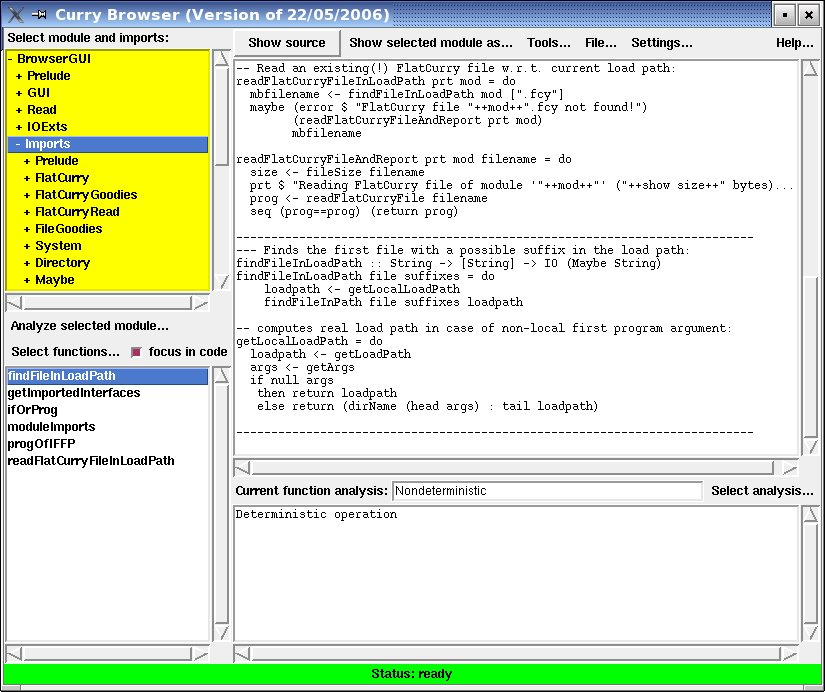
\includegraphics[scale=0.7]{currybrowser.jpg}
\end{center}
\caption{Snapshot of the main window of CurryBrowser\label{fig-currybrowser}}
\end{figure}
%
To get an impression of the use of \cb, Figure~\ref{fig-currybrowser}
shows a snapshot of its use on a particular application
(here: the implementation of \cb).
The upper list box in the left column shows the modules and their imports
in order to browse through the modules of an application.
Similarly to directory browsers, the list of imported modules of a module
can be opened or closed by clicking.
After selecting a module in the list of modules, its source code,
interface, or various other formats of the module can be shown
in the main (right) text area. For instance, one can show
pretty-printed versions of the intermediate flat programs (see below)
in order to see how local function definitions are translated by lambda lifting
\cite{Johnsson85}
or pattern matching is translated into case expressions \cite{Hanus97POPL,Wadler87}.
Since Curry is a language with parametric polymorphism and type inference,
programmers often omit the type signatures when defining functions.
Therefore, one can also view (and store) the selected module as source code where
missing type signatures are added.

Below the list box for selecting modules, there is a menu
(``Analyze selected module'') to analyze all functions
of the currently selected module at once. This is useful
to spot some functions of a module that could be problematic
in some application contexts, like functions that are impure (i.e., the result
depends on the evaluation time) or partially defined (i.e.,
not evaluable on all ground terms).
If such an analysis is selected,
the names of all functions are shown in the
lower list box of the left column (the ``function list'')
with prefixes indicating the properties of the individual functions.

The function list box can be also filled with functions
via the menu ``Select functions''. For instance, all functions
or only the exported functions defined in the currently selected
module can be shown there, or all functions from different modules
that are directly or indirectly called from
a currently selected function.
This list box is central to focus on a function in the
source code of some module or to analyze some function,
i.e., showing their properties. In order to focus on a function,
it is sufficient to check the ``focus on code'' button.
To analyze an individually selected function, one can
select an analysis from the list of available program analyses
(through the menu ``Select analysis'').
In this case, the analysis results are either shown
in the text box below the main text area
or visualized by separate tools, e.g., by a graph drawing tool for
visualizing call graphs.
Some analyses are local, i.e., they need only to consider the local definition
of this function (e.g., ``Calls directly,'' ``Overlapping rules,''
``Pattern completeness''),
where other analyses are global, i.e.,
they consider the definitions of all functions directly or indirectly called
by this function (e.g., ``Depends on,'' ``Solution complete,''
``Set-valued'').
%
Finally, there are a few additional tools integrated into \cb,
for instance, to visualize the import relation between all modules
as a dependency graph. These tools are available through the ``Tools'' menu.

More details about the use of \cb and all built-in analyses
are available through the ``Help'' menu of \cb.


\newpage

\section{CurryTest: A Tool for Testing Curry Programs}
\label{sec-currytest}

CurryTest\index{CurryTest}\index{testing programs}\index{program!testing}
is a simple tool in the PAKCS distribution to write
and run repeatable tests. CurryTest simplifies the task
of writing test cases for a module and executing them.
The tool is easy to use. Assume one has implemented a module \code{MyMod}
and wants to write some test cases to test its functionality,
making regression tests in future versions, etc.
For this purpose, there is a system library \code{Assertion}
(Section~\ref{Library:Assertion}) which
contains the necessary definitions for writing tests.
In particular, it exports an abstract polymorphic type \ccode{Assertion a}
together with the following operations:
\startprog
assertTrue      :: String -> Bool -> Assertion ()
assertEqual     :: String -> a -> a -> Assertion a
assertValues    :: String -> a -> [a] -> Assertion a
assertSolutions :: String -> (a->Success) -> [a] -> Assertion a
assertIO        :: String -> IO a -> a -> Assertion a
assertEqualIO   :: String -> IO a -> IO a -> Assertion a
\stopprog
The expression \ccode{assertTrue $s$ $b$}
is an assertion (named $s$) that the expression $b$ has the value \code{True}.
Similarly, the expression \ccode{assertEqual $s$ $e_1$ $e_2$}
asserts that the expressions $e_1$ and $e_2$
must be equal (i.e., \code{$e_1$==$e_2$} must hold),
the expression \ccode{assertValues $s$ $e$ $vs$} asserts
that $vs$ is the multiset of all values of $e$,
and the expression \ccode{assertSolutions $s$ $c$ $vs$} asserts
that the constraint abstraction $c$ has the multiset of solutions $vs$.
Furthermore, the expression \ccode{assertIO $s$ $a$ $v$}
asserts that the I/O action $a$ yields the value $v$ whenever it is
executed, and
the expression \ccode{assertEqualIO $s$ $a_1$ $a_2$}
asserts that the I/O actions $a_1$ and $a_2$ yields equal values.
The name $s$ provided as a first argument in each assertion
is used in the protocol produced by the test tool.

One can define a test program by importing the module
to be tested together with the module \code{Assertion} and defining
top-level functions of type \code{Assertion} in this module
(which must also be exported).
As an example, consider the following program
that can be used to test some list processing functions:
\startprog
\medskip
import List
import Assertion
\medskip
test1 = assertEqual     "++"     ([1,2]++[3,4]) [1,2,3,4]
\medskip
test2 = assertTrue      "all"    (all (<5) [1,2,3,4])
\medskip
test3 = assertSolutions "prefix" (\labs{}x -> let y free in  x\,++\,y =:= [1,2])
                                 [[],[1],[1,2]]
\medskip
\stopprog
For instance, \code{test1} asserts that the result of evaluating the
expression \code{([1,2]++[3,4])} is equal to \code{[1,2,3,4]}.

We can execute a test suite by the command\pindex{currytest}
\startprog
currytest testList
\stopprog
(\code{currytest} is a program stored in \code{$pakcshome$/bin}
where $pakcshome$ is the installation directory of PAKCS;
see Section~\ref{sec-general}).
In our example, \ccode{testList.curry} is the program containing the
definition of all assertions. This has the effect
that all exported top-level functions
of type \code{Assertion} are tested (i.e., the corresponding
assertions are checked) and the results
(\ccode{OK} or failure) are reported together with the name of each assertion.
%If failures occur, the complete test results are also
%written into a file named \ccode{testList.testlog}.''
For our example above, we obtain the following successful protocol:
\startprog
============================================================
Testing module "testList"...
OK: ++
OK: all
OK: prefix
All tests successfully passed.
============================================================
\stopprog
There is also a graphical interface that summarizes the results
more nicely.\footnote{Due to a bug in older versions of SICStus-Prolog,
it works only with SICStus-Prolog version 3.8.5 (or newer).}
In order to start this interface, one has to add the parameter
\ccode{--window} (or \ccode{-w}), e.g., executing a test suite by
\startprog
currytest --window testList
\stopprog
or
\startprog
currytest -w testList
\stopprog
A snapshot of the interface is shown in Figure~\ref{fig-currytest}.

\begin{figure}%[t]
\begin{center}
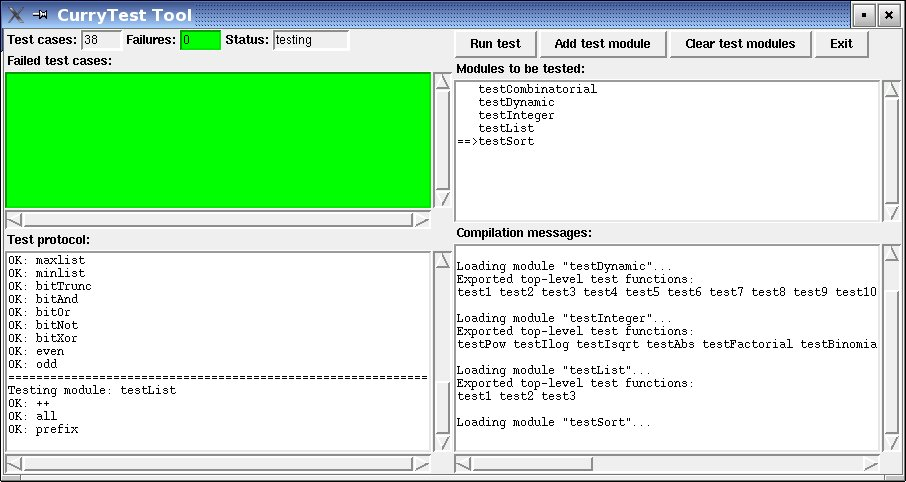
\includegraphics[scale=0.7]{currytest.jpg}
\end{center}
\caption{Snapshot of CurryTest's graphical interface\label{fig-currytest}}
\end{figure}


\newpage

\section{ERD2Curry: A Tool to Generate Programs from ER Specifications}
\label{sec-erd2curry}

ERD2Curry\index{ERD2Curry}\index{database programming}
is a tool to generate Curry code to access and manipulate data
persistently stored from
entity relationship diagrams.\index{entity relationship diagrams}
The idea of this tool is described in detail in
\cite{BrasselHanusMueller08PADL}.
Thus, we describe only the basic steps to use this tool
in the following.

If one creates an entity relationship diagram (ERD)
with the Umbrello UML Modeller, one has to store its
XML description in XMI format (as offered by Umbrello)
in a file, e.g., \ccode{myerd.xmi}.
This description can be compiled into a Curry program by the
command\pindex{erd2curry}
\startprog
erd2curry myerd.xmi
\stopprog
(\code{erd2curry} is a program stored in \code{$pakcshome$/bin}
where $pakcshome$ is the installation directory of PAKCS;
see Section~\ref{sec-general}).
If \code{MyData} is the name of the ERD, the Curry program file
\ccode{MyData.curry} is generated containing all the necessary
database access code as described in \cite{BrasselHanusMueller08PADL}.

If one does not want to use the Umbrello UML Modeller,
one can also create a textual description of the ERD
as a Curry term of type \code{ERD}
(w.r.t.\ the type definition given in module
\code{$pakcshome$/tools/erd2curry/ERD.curry})
and store it in some file, e.g., \ccode{myerd.term}.
This description can be compiled into a Curry program by the
command\pindex{erd2curry}
\startprog
erd2curry -t myerd.term
\stopprog
%
There is also the possibility to visualize an ERD term
as a graph with the graph visualization program \code{dotty}
(for this purpose, it might be necessary to adapt the definition
of the operation \code{dotCmd} in
\code{$pakcshome$/tools/erd2curry/ERD2Graph.curry}
according to your local environment).
This can be done by the command
\startprog
erd2curry -v myerd.term
\stopprog

\paragraph{Inclusion in the Curry application:}
To compile the generated database code, either
include the directory \code{$pakcshome$/tools/erd2curry}
into your Curry load path
(e.g., by setting  the environment variable
\ccode{CURRYPATH}\pindex{CURRYPATH}, see also Section~\ref{sec-modules})
or copy the file
\code{$pakcshome$/tools/erd2curry/ERDGeneric.curry}
into the directory of the generated database code.


\newpage

\section{UI: Declarative Programming of User Interfaces}
\label{sec-ui}

The PAKCS distribution contains a collection of libraries
to implement graphical user interfaces\index{user interface}
as well as web-based user interfaces
from declarative descriptions.
Exploiting these libraries, it is possible
to define the structure and functionality of a user interface
independent from the concrete technology.
Thus, a graphical user interface or a web-based user interface
can be generated from the same description by simply changing
the imported libraries.
This programming technique is described in detail in
\cite{HanusKluss09PADL}.

The libraries implementing these user interfaces are contained
in the directory
\startprog
$pakcshome$/tools/ui
\stopprog
Thus, in order to compile programs containing such user interface
specifications, one has to
include the directory \code{$pakcshome$/tools/ui}
into the Curry load path
(e.g., by setting  the environment variable
\ccode{CURRYPATH}\pindex{CURRYPATH}, see also Section~\ref{sec-modules}).
The directory
\startprog
$pakcshome$/tools/ui/examples
\stopprog
contains a few examples for such user interface specifications.


\newpage

\section{Preprocessing FlatCurry Files}
\label{sec-pakcspp}

The current parser allows to apply transformations on the intermediate
FlatCurry files after they are generated from the
corresponding Curry source file.
Currently, only the FlatCurry file corresponding to the main module
can be transformed.

A transformation can be specified as follows:
\begin{enumerate}
\item {\bf Options to \code{pakcs/bin/parsecurry}:}
\begin{description}
\item[\fbox{\code{--fpopt}}]\pindex{-fpopt}
Apply functional pattern optimization
(see \code{pakcs/tools/optimize/NonStrictOpt.curry} for details).

\item[\fbox{\code{--compact}}]\pindex{--compact}
Apply code compactification after parsing, i.e., transform the main
module and all its imported into one module and delete all
non-accessible functions.

\item[\fbox{\code{--compactexport}}]
Similar to \code{--compact} but delete all functions that are not accessible
from the exported functions of the main module.

\item[\fbox{\code{--compactmain:f}}]
Similar to \code{--compact} but delete all functions that are not accessible
from the function \ccode{f} of the main module.

\item[\fbox{\code{--fcypp cmd}}]\pindex{--fcypp}
Apply command \code{cmd} to the main module after parsing. This is useful to
integrate your own transformation into the compilation process.
Note that the command \ccode{cmd prog} should perform a transformation
on the FlatCurry file \code{prog.fcy}, i.e., it replaces the FlatCurry
file by a new one.
\end{description}

\item {\bf Setting the environment variable \code{FCYPP}:}\pindex{FCYPP}\\
For instance, setting \code{FCYPP} by
\startprog
export FCYPP="--fpopt"
\stopprog
will apply the functional pattern optimization if programs are compiled
and loaded in the PAKCS programming environment.


\item {\bf Putting options into the source code:}\pindex{PAKCS_OPTION_FCYPP}\\
If the source code contains a line with a comment of the form (the comment
must start at the beginning of the line)
\startprog
\{-\# PAKCS_OPTION_FCYPP <options> \#-\}
\stopprog
then the transformations specified by \code{<options>} are applied after
translating the source code into FlatCurry code. For instance,
the functional pattern optimization can be set by the comment
\startprog
\{-\# PAKCS_OPTION_FCYPP --fpopt \#-\}
\stopprog
in the source code. Note that this comment must be in a single line 
of the source program. If there are multiple lines containing such comments,
only the first one will be considered.
\end{enumerate}
\paragraph{Multiple options:}
Note that an arbitrary number of transformations can be specified
by the methods described above.
If several specifications for preprocessing FlatCurry files are used,
they are executed in the following order:
\begin{enumerate}
\item all transformations specified by the environemnt variable
\code{FCYPP} (from left to right)
\item all transformations specified as command line options of parsecurry
   (from left to right)
\item all transformations specified by a comment line in the source code
   (from left to right)
\end{enumerate}


\newpage

\section{Technical Problems}

Due to the fact that Curry is intended to implement
distributed systems (see Appendix~\ref{sec-ports}),
it might be possible that some technical problems
arise due to the use of sockets for implementing these
features. Therefore, this section gives some information
about the technical requirements of PAKCS and how to solve
problems due to these requirements.

There is one fixed port that is used by the implementation of PAKCS:
\begin{description}
\item[Port 8766:] This port is used by the
{\bf Curry Port Name Server} (CPNS) to implement symbolic names for
ports in Curry (see Appendix~\ref{sec-ports}).
If some other process uses this port on the machine,
the distribution facilities defined in the module \code{Ports}
(see Appendix~\ref{sec-ports}) cannot be used.
\end{description}
If these features do not work, you can try to find out
whether this port is in use by the shell command
\ccode{netstat -a | fgrep 8766} (or similar).

The CPNS is implemented as a demon listening on its port 8766
in order to serve requests about registering a new symbolic
name for a Curry port or asking the physical port number
of a Curry port. The demon will be automatically started for
the first time on a machine when a user compiles a program
using Curry ports. It can also be manually started and terminated by the
scripts \code{$pakcshome$/cpns/start} and
\code{$pakcshome$/cpns/stop}.
If the demon is already running, the command \code{$pakcshome$/cpns/start}
does nothing (so it can be always executed
before invoking a Curry program using ports).

If you detect any further technical problem,
please write to
\begin{center}
\code{mh@informatik.uni-kiel.de}
\end{center}

\newpage

\addcontentsline{toc}{section}{Bibliography}
\bibliography{manual}
\bibliographystyle{plain}

\newpage
\appendix

\section{Libraries of the PAKCS Distribution}
\label{sec:libraries}

{\setlength{\parindent}{0.0cm}

The PAKCS compiler system provides an extensive collection
of libraries for application programming.
The libraries for arithmetic constraints over real numbers,
finite domain constraints,
ports for concurrent and distributed programming, and
meta-programming by representing Curry programs in Curry
are described in the following subsection in more detail.
The complete set of libraries with all exported types and functions
are described in the further subsections.
For a more detailed online documentation of all libraries of PAKCS,
see \url{http://www.informatik.uni-kiel.de/~pakcs/lib/index.html}.

\subsection{Constraints, Ports, Meta-Programming}

\subsubsection{Arithmetic Constraints}

The primitive entities for the use of arithmetic constraints
are defined in the system module \code{CLPR}
(cf.\ Section~\ref{sec-modules}), i.e., in order to use them,
the program must contain the import declaration
\startprog
import CLPR
\stopprog
Floating point arithmetic is supported in PAKCS
via arithmetic constraints, i.e., the equational constraint
\ccode{2.3 +.~x =:= 5.5} is solved by binding \code{x} to \code{3.2}
(rather than suspending the evaluation of the addition,
as in corresponding constraints on integers like
\ccode{3+x=:=5}). All operations related to
floating point numbers are suffixed by \ccode{.}.
The following functions and constraints on floating point
numbers are supported in PAKCS:
\begin{description}
\item[\code{(+.)   :: Float -> Float -> Float}]~\\
Addition on floating point numbers.
\item[\code{(-.)   :: Float -> Float -> Float}]~\\
Subtraction on floating point numbers.
\item[\code{(*.)   :: Float -> Float -> Float}]~\\
Multiplication on floating point numbers.
\item[\code{(/.)   :: Float -> Float -> Float}]~\\
Division on floating point numbers.
\item[\code{(<.)   :: Float -> Float -> Success}]~\\
Comparing two floating point numbers with the ``less than'' relation.
\item[\code{(>.)   :: Float -> Float -> Success}]~\\
Comparing two floating point numbers with the ``greater than'' relation.
\item[\code{(<=.)  :: Float -> Float -> Success}]~\\
Comparing two floating point numbers with the ``less than or equal'' relation.
\item[\code{(>=.)  :: Float -> Float -> Success}]~\\
Comparing two floating point numbers with the ``greater than or equal''
relation.
\item[\code{i2f    :: Int -> Float}]~\\
Converting an integer number into a floating point number.
\end{description}
As an example, consider a constraint \code{mortgage}
which relates the principal \code{p},
the lifetime of the mortgage in months \code{t},
the monthly interest rate \code{ir},
the monthly repayment \code{r},
and the outstanding balance at the end of the lifetime \code{b}.
The financial calculations
can be defined by the following two rules in Curry (the second rule
describes the repeated accumulation of the interest):
\startprog
~
import CLPR
~
mortgage p t ir r b | t >. 0.0 \& t <=. 1.0  --lifetime not more than 1 month?
                    =  b =:= p *. (1.0 +. t *. ir) -. t*.r \vspace{1ex}
mortgage p t ir r b | t >. 1.0               --lifetime more than 1 month?
                    =  mortgage (p *. (1.0+.ir)-.r) (t-.1.0) ir r b
~
\stopprog
Then we can calculate the monthly payment for paying back
a loan of \$100,000 in 15 years with a monthly interest rate of 1\%
by solving the goal
\startprog
mortgage 100000.0 180.0 0.01 r 0.0
\stopprog
which yields the solution \code{r=1200.17}.

Note that only linear arithmetic equalities or inequalities
are solved by the constraint solver. Non-linear constraints
like \ccode{x *.~x =:= 4.0} are suspended until they become
linear.


\subsubsection{Finite Domain Constraints}

Finite domain constraints are constraints where all variables
can only take a finite number of possible values.
For simplicity, the domain of finite domain variables are
identified with a subset of the integers, i.e., the type
of a finite domain variable is \code{Int}. The arithmetic
operations related to finite domain variables are suffixed by \ccode{\#}.
The following functions and constraints for finite domain constraint solving
are currently supported in PAKCS:\footnote{Note that
this library is based on the corresponding library of SICStus-Prolog
but does not implement the complete functionality of the SICStus-Prolog library.
However, using the PAKCS interface for external functions (see
Appendix~\ref{sec-external-functions}), it is relatively
easy to provide the complete functionality.}

\begin{description}
\item[\code{domain :: [Int] -> Int -> Int -> Success}]~\\
The constraint \ccode{domain [$x_1,\ldots,x_n$] $l$ $u$}
is satisfied if the domain of all variables $x_i$ is the interval $[l,u]$.
\item[\code{(+\#)   :: Int -> Int -> Int}]~\\
Addition on finite domain values.
\item[\code{(-\#)   :: Int -> Int -> Int}]~\\
Subtraction on finite domain values.
\item[\code{(*\#)   :: Int -> Int -> Int}]~\\
Multiplication on finite domain values.
\item[\code{(=\#)   :: Int -> Int -> Success}]~\\
Equality of finite domain values.
\item[\code{(/=\#)  :: Int -> Int -> Success}]~\\
Disequality of finite domain values.
\item[\code{(<\#)   :: Int -> Int -> Success}]~\\
``less than'' relation on finite domain values.
\item[\code{(<=\#)  :: Int -> Int -> Success}]~\\
``less than or equal'' relation on finite domain values.
\item[\code{(>\#)   :: Int -> Int -> Success}]~\\
``greater than'' relation on finite domain values.
\item[\code{(>=\#)  :: Int -> Int -> Success}]~\\
``greater than or equal'' relation on finite domain values.
\item[\code{sum :: [Int] -> (Int -> Int -> Success) -> Int -> Success}]~\\
The constraint \ccode{sum [$x_1,\ldots,x_n$] $op$ $x$}
is satisfied if all $x_1+\cdots + x_n \mathrel{op} x$ is satisfied,
where $op$ is one of the above finite domain constraint relations
(e.g., \ccode{=\#}).
\item[\code{scalar_product :: [Int] -> [Int] -> (Int -> Int -> Success) -> Int -> Success}]~\\
The constraint \ccode{scalar_product [$c_1,\ldots,c_n$] [$x_1,\ldots,x_n$] $op$ $x$}
is satisfied if all $c_1 x_1+\cdots + c_n x_n \mathrel{op} x$ is satisfied,
where $op$ is one of the above finite domain constraint relations.
\item[\code{count :: Int -> [Int] -> (Int -> Int -> Success) -> Int -> Success}]~\\
The constraint \ccode{count $k$ [$x_1,\ldots,x_n$] $op$ $x$}
is satisfied if all $k \mathrel{op} x$ is satisfied,
where $n$ is the number of the $x_i$ that are equal to $k$ and
$op$ is one of the above finite domain constraint relations.
\item[\code{all_different :: [Int] -> Success}]~\\
The constraint \ccode{all_different [$x_1,\ldots,x_n$]}
is satisfied if all $x_i$ have pairwise different values.
\item[\code{labeling :: [LabelingOption] -> [Int] -> Success}]~\\
The constraint \ccode{labeling $os$ [$x_1,\ldots,x_n$]}
non-deterministically instantiates all $x_i$ to the values
of their domain according to the options $os$ (see the module documentation
for further details about these options).
\end{description}
These entities are defined in the system module \code{CLPFD}
(cf.\ Section~\ref{sec-modules}), i.e., in order to use it,
the program must contain the import declaration
\startprog
import CLPFD
\stopprog
As an example, consider the classical \ccode{send+more=money} problem
where each letter must be replaced by a different digit such that this
equation is valid and there are no leading zeros.
The usual way to solve finite domain constraint problems
is to specify the domain of the involved variables followed
by a specification of the constraints and the labeling
of the constraint variables in order to start the search for solutions.
Thus, the \ccode{send+more=money} problem can be solved as follows:
\startprog
~
import CLPFD
~
smm l =
        l =:= [s,e,n,d,m,o,r,y] \&
        domain l 0 9 \&
        s >\# 0 \&
        m >\# 0 \&
        all_different l  \&
                         1000 *\# s +\# 100 *\# e +\# 10 *\# n +\# d
        +\#               1000 *\# m +\# 100 *\# o +\# 10 *\# r +\# e
        =\# 10000 *\# m +\# 1000 *\# o +\# 100 *\# n +\# 10 *\# e +\# y \&
        labeling [FirstFail] l
        where s,e,n,d,m,o,r,y free
~
\stopprog
Then we can solve this problem by evaluating the goal
\ccode{smm [s,e,n,d,m,o,r,y]} which yields the unique solution
\code{\{s=9,e=5,n=6,d=7,m=1,o=0,r=8,y=2\}}.


\subsubsection{Ports: Distributed Programming in Curry}
\label{sec-ports}

To support the development of concurrent and distributed applications,
PAKCS supports internal and external ports\index{ports} as
described in \cite{Hanus99PPDP}.
Since \cite{Hanus99PPDP} contains a detailed description of this
concept together with various programming examples, we only summarize here
the functions and constraints supported for ports in PAKCS.

The basic datatypes, functions, and constraints for ports
are defined in the system module \code{Ports}
(cf.\ Section~\ref{sec-modules}), i.e., in order to use ports,
the program must contain the import declaration
\startprog
import Ports
\stopprog
This declaration includes the following entities in the program:
\begin{description}
\item[\code{Port a}\pindex{Port}]~\\
This is the datatype of a port to which one can send messages of type \code{a}.

\item[\code{openPort :: Port a -> [a] -> Success}]~\\
The constraint \ccode{openPort p s}\pindex{openPort}
establishes a new \emph{internal port}
\code{p} with an associated message stream \code{s}. \code{p} and \code{s} must be
unbound variables,
otherwise the constraint fails (and causes a runtime error).

\item[\code{send :: a -> Port a -> Success}]~\\
The constraint \ccode{send m p}\pindex{send}
is satisfied if \code{p} is constrained
to contain the message \code{m}, i.e., \code{m} will be sent to the port
\code{p} so that it appears in the corresponding stream.

\item[\code{doSend :: a -> Port a -> IO ()}]~\\
The I/O action \ccode{doSend m p}\pindex{doSend} solves the constraint
\ccode{send m p} and returns nothing.

\item[\code{openNamedPort :: String -> IO [a]}]~\\
The I/O action \ccode{openNamedPort n}\pindex{openNamedPort}
opens a new \emph{external port} with
symbolic name \code{n} and returns the associated stream of messages.

\item[\code{connectPort :: String -> IO (Port a)}]~\\
The I/O action \ccode{connectPort n}\pindex{connectPort}
returns a port with symbolic name
\code{n} (i.e., \code{n} must have the form ``\emph{portname@machine})
to which one can send messages by the \code{send} constraint.
Currently, no dynamic type checking is done for external ports,
i.e., sending messages of the wrong type to a port might lead to
a failure of the receiver.
\end{description}

\paragraph{Restrictions:}
Every expression, possibly containing logical variables, can be sent to
a port. However, as discussed in \cite{Hanus99PPDP},
port communication is strict, i.e., the expression is
evaluated to normal form before sending it by the
constraint \code{send}. Furthermore, if messages containing
logical variables are sent to \emph{external ports},
the behavior is as follows:
\begin{enumerate}
\item The sender waits until all logical variables in the message
have been bound by the receiver.
\item The binding of a logical variable received by a process
is sent back to the sender of this logical variable only if
it is bound to a \emph{ground} term, i.e., as long as the binding contains
logical variables, the sender is not informed about the binding
and, therefore, the sender waits.
\end{enumerate}

\paragraph{External ports on local machines:}
The implementation of external ports assumes that the
host machine running the application is connected to the Internet
(i.e., it uses the standard IP address of the host machine
for message sending). If this is not the case and the application
should be tested by using external ports only on the local host
without a connection to the Internet,
the environment variable \ccode{PAKCS_LOCALHOST}\pindex{PAKCS_LOCALHOST}
must be set to \ccode{yes}
\emph{before PAKCS system is started}.
In this case, the IP address \code{127.0.0.1} and the hostname
\ccode{localhost} are used for identifying the local machine.

\paragraph{Selection of Unix sockets for external ports:}
The implementation of ports uses sockets to communicate
messages sent to external ports.
Thus, if a Curry program uses the
I/O action \code{openNamedPort}\pindex{openNamedPort}
to establish an externally visible server,
PAKCS selects a Unix socket for the port communication.
Usually, a free socket is selected by the operating system.
If the socket number should be fixed in an application (e.g.,
because of the use of firewalls\index{firewall} that allow only
communication over particular sockets), then one
can set the environment variable \ccode{PAKCS_SOCKET}\pindex{PAKCS_SOCKET}
to a distinguished socket number before the PAKCS system is started.
This has the effect that PAKCS uses only this socket
number for communication (even for several external ports
used in the same application program).

\paragraph{Debugging:}
To debug distributed systems,
it is sometimes helpful to see all messages sent to external ports.
This is supported by the environment variable
\ccode{PAKCS_TRACEPORTS}.\pindex{PAKCS_TRACEPORTS}
If this variable is set to \ccode{yes}
\emph{before the PAKCS system is started}, then all
connections to external ports and all
messages sent and received on external ports are
printed on the standard error stream.


\subsubsection{AbstractCurry and FlatCurry: Meta-Programming in Curry}
\label{sec-flatcurry}

\index{AbstractCurry}
\index{FlatCurry}
To support meta-programming, i.e., the manipulation of Curry programs
in Curry, there are system modules \code{FlatCurry} and \code{AbstractCurry}
(stored in the directory \ccode{$pakcshome$/lib/meta})
which define datatypes for the representation
of Curry programs.
\code{AbstractCurry} is a more direct representation of a Curry program,
whereas \code{FlatCurry} is a simplified representation
where local function definitions are replaced by global definitions
(i.e., lambda lifting has been performed) and pattern matching
is translated into explicit case/or expressions.
Thus, \code{FlatCurry} can be used for more back-end oriented
program manipulations (or, for writing new back ends for Curry),
whereas \code{AbstractCurry} is intended for manipulations of
programs that are more oriented towards the source program.

Both modules contain predefined I/O actions to read programs
in the \code{AbstractCurry} (\code{readCurry}\pindex{readCurry})
or \code{FlatCurry}
(\code{readFlatCurry}\pindex{readFlatCurry}) format.
These actions parse the corresponding source program and return
a data term representing this program (according to the definitions
in the modules \code{AbstractCurry} and \code{FlatCurry}).

Since all datatypes are explained in detail in these modules,
we refer to the online documentation\footnote{%
\url{http://www.informatik.uni-kiel.de/~pakcs/lib/CDOC/FlatCurry.html} and
\url{http://www.informatik.uni-kiel.de/~pakcs/lib/CDOC/AbstractCurry.html}}
of these modules.

As an example, consider a program file \ccode{test.curry}
containing the following two lines:
\startprog
rev []     = []
rev (x:xs) = (rev xs) ++ [x]
\stopprog
Then the I/O action \code{(FlatCurry.readFlatCurry "test")} returns the
following term:
\startprog
 (Prog "test"
  ["Prelude"]
  []
  [Func ("test","rev") 1 Public
        (FuncType (TCons ("Prelude","[]") [(TVar 0)])
                  (TCons ("Prelude","[]") [(TVar 0)]))
        (Rule [0]
           (Case Flex (Var 0)
              [Branch (Pattern ("Prelude","[]") [])
                  (Comb ConsCall ("Prelude","[]") []),
               Branch (Pattern ("Prelude",":") [1,2])
                  (Comb FuncCall ("Prelude","++")
                        [Comb FuncCall ("test","rev") [Var 2],
                         Comb ConsCall ("Prelude",":")
                              [Var 1,Comb ConsCall ("Prelude","[]") []]
                        ])
              ]))]
  []
 )
\stopprog


%%%%%%%%%%%%%%%%%%%%%%%%%%%%%%%%%%%%%%%%%%%%%%%%%%%%%%%%%%%%%%%%%%%%%%%%%
% Definitions in order to LaTeX documents generated by "currydoc --tex"
%%%%%%%%%%%%%%%%%%%%%%%%%%%%%%%%%%%%%%%%%%%%%%%%%%%%%%%%%%%%%%%%%%%%%%%%%

\newcommand{\currymodule}[1]{\subsubsection{Library #1}\label{Library:#1}}
\newcommand{\currytypesstart}{\subsubsection*{Exported types:}}
\newcommand{\currytypesstop}{}
\newcommand{\currytypesynstart}[2]{{\tt type #2}\pindex{#1} \begin{quote}}
\newcommand{\currytypesynstop}{\end{quote}}
\newcommand{\currydatastart}[1]{{\tt data #1}\pindex{#1} \begin{quote}}
\newcommand{\currydatacons}{\end{quote}%
\begin{itemize}\item[] \hspace{-4ex}\emph{Exported constructors:}}
\newcommand{\currydatastop}{\end{itemize}}
\newcommand{\curryconsstart}[2]{\item {\tt #1~::~#2}\par}
\newcommand{\curryfuncstart}{\subsubsection*{Exported functions:}}
\newcommand{\curryfuncstop}{}
\newcommand{\curryfunctionstart}[2]{#2\pindex{#1}\begin{quote}}
\newcommand{\curryfunctionstop}{\end{quote}}
\newcommand{\curryfuncsig}[2]{{\tt #1~::~#2}}


\subsection{General Libraries}

\input{lib/AllSolutions}
\input{lib/Assertion}
\input{lib/Char}
\input{lib/CLPFD}
\input{lib/CLPR}
\input{lib/CLPB}
\input{lib/Combinatorial}
\input{lib/Constraint}
\input{lib/CSV}
\input{lib/Database}
\input{lib/DaVinci}
\input{lib/Directory}
\input{lib/Dynamic}
\input{lib/FileGoodies}
\input{lib/Float}
\input{lib/Global}
\input{lib/GlobalVariable}
\input{lib/GUI}
\input{lib/Integer}
\input{lib/IO}
\input{lib/IOExts}
\input{lib/JavaScript}
\input{lib/KeyDatabase}
\input{lib/KeyDatabaseSQLite}
\input{lib/KeyDB}
\input{lib/List}
\input{lib/Maybe}
\input{lib/NamedSocket}
\input{lib/Parser}
\input{lib/Ports}
\input{lib/Pretty}
\input{lib/Profile}
\input{lib/PropertyFile}
\input{lib/Read}
\input{lib/ReadNumeric}
\input{lib/ReadShowTerm}
\input{lib/SetFunctions}
\input{lib/Socket}
\input{lib/System}
\input{lib/Time}
%\input{lib/Tk}
\input{lib/Unsafe}


\subsection{Data Structures and Algorithms}

\input{lib/Array}
\input{lib/Dequeue}
\input{lib/FiniteMap}
\input{lib/GraphInductive}
\input{lib/Random}
\input{lib/RedBlackTree}
\input{lib/SetRBT}
\input{lib/Sort}
\input{lib/TableRBT}
\input{lib/Traversal}

\subsection{Libraries for Web Applications}

\input{lib/CategorizedHtmlList}
\input{lib/HTML}
\input{lib/HtmlParser}
\input{lib/Mail}
\input{lib/Markdown}
\input{lib/WUI}
\input{lib/URL}
\input{lib/XML}
\input{lib/XmlConv}

\subsection{Libraries for Meta-Programming}

\input{lib/AbstractCurry}
\input{lib/AbstractCurryPrinter}
\input{lib/CompactFlatCurry}
\input{lib/CurryStringClassifier}
\input{lib/FlatCurry}
\input{lib/FlatCurryGoodies}
\input{lib/FlatCurryRead}
\input{lib/FlatCurryShow}
\input{lib/FlatCurryTools}
\input{lib/FlatCurryXML}
\input{lib/FlexRigid}
\input{lib/PrettyAbstract}

} % end setlength parindent

\newpage

\input{markdown_syntax}

\newpage

\begin{figure}%[t]
\begin{center}
 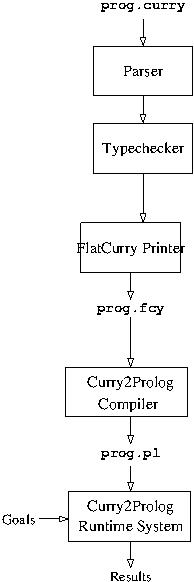
\includegraphics[scale=0.85]{pakcs_overview.jpg}
\end{center}\vspace{-5ex}
\caption{Overview of PAKCS\label{fig-pakcs}}
\end{figure}

\section{Overview of the PAKCS Distribution}

A schematic overview of the various components contained in
the distribution of PAKCS and the
translation process of programs inside PAKCS is shown in
Figure~\ref{fig-pakcs} on page~\pageref{fig-pakcs}.
In this figure, boxes denote different components of PAKCS
and names in boldface denote files containing
various intermediate representations during the translation
process (see Section~\ref{sec-auxfiles} below).
The PAKCS distribution contains a front end for reading (parsing and
type checking) Curry programs that can be also used by
other Curry implementations.
The back end (formerly known as ``Curry2Prolog''\index{Curry2Prolog})
compiles Curry programs into Prolog programs.
It also support constraint solvers for
arithmetic constraints over real numbers and finite domain constraints,
and further libraries for GUI programming, meta-programming etc.
Currently, it does not implement encapsulated search in full generality
(only a strict version of \code{findall} is supported),
and concurrent threads are not executed in a fair manner.


\newpage

\section{Auxiliary Files}
\label{sec-auxfiles}

During the translation and execution of a Curry program with PAKCS,
various intermediate representations of the source program are created
and stored in different files which are shortly explained in this section.
If you use the PAKCS, it is not necessary to know about
these auxiliary files because they are automatically generated
and updated. You should only remember the command for deleting
all auxiliary files (\ccode{cleancurry}, see Section~\ref{sec-general})
to clean up your directories.

The various components of PAKCS create
the following auxiliary files.
\begin{description}
\item[\code{prog.fcy}:] This file contains the Curry program
in the so-called ``FlatCurry'' representation where all functions are global
(i.e., lambda lifting has been performed) and pattern matching
is translated into explicit case/or expressions
(compare Appendix~\ref{sec-flatcurry}).
This representation might be useful for other back ends and
compilers for Curry and is the basis doing meta-programming in Curry.
This file is implicitly
generated when a program is read by PAKCS.
It can be also explicitly generated by the command\pindex{parsecurry}
\startprog
parsecurry --flat prog
\stopprog
The FlatCurry representation of a Curry program is usually
generated by the front-end after parsing, type checking and eliminating
local declarations.
If $dir$ is the directory where the Curry program is stored,
the corresponding FlatCurry program is stored in the directory
\ccode{$dir$/.curry}.

\item[\code{prog.fint}:] This file contains the interface
of the program in the so-called ``FlatCurry'' representation,
i.e., it is similar to \code{prog.fcy} but contains only exported
entities and the bodies of all functions omitted (i.e., ``external'').
This representation is useful for providing a fast access
to module interfaces.
This file is implicitly generated by the command\pindex{parsecurry}
\startprog
parsecurry --flat prog
\stopprog
and stored in the same directory as \code{prog.fcy}.

\item[\code{prog.pl}:] This file contains a Prolog program
as the result of translating the Curry program with PAKCS.
If $dir$ is the directory where the Curry program is stored,
the corresponding Prolog program is stored in the directory
\ccode{$dir$/.curry/.pakcs}.

\item[\code{prog.po}:] This file contains the Prolog program
\code{prog.pl} in an intermediate format for faster loading.
This file is stored in the same directory as \code{prog.pl}.

\item[\code{prog.state}:] This file contains the saved state
after compiling and saving a program with PAKCS
(see Section~\ref{sec-use-curry2prolog}).

\end{description}


\newpage


\section{Changing the Prelude or System Modules}

The standard prelude, which is automatically imported into each Curry program,
and all system modules containing datatypes and functions
useful for application programming
(cf.\ Appendix~\ref{sec:libraries})
are stored in the system module directory \ccode{$pakcshome$/lib}
(and its subdirectories).
If you change any of these modules,
you have to recompile the complete system by
executing \code{make} in the directory $pakcshome$.



\newpage

\section{External Functions}
\label{sec-external-functions}

\index{function!external}\index{external function}
Currently, PAKCS has no general interface to external functions.
Therefore, if a new external function should be added
to the system, this function must be declared as \code{external}
in the Curry source code
and then an implementation for this external function
must be inserted in the corresponding back end.
An external function is defined as follows in the Curry source code:
\begin{enumerate}
\item
Add a type declaration for the external function somewhere
in the body of the appropriate file (usually, the prelude
or some system module).
\item
For external functions it is not allowed to define any
rule since their semantics is determined by an external implementation.
Instead of the defining rules, you have to write
\startprog
f external
\stopprog
somewhere in the file containing the type declaration for 
the external function \code{f}.
\end{enumerate}
For instance, the addition on integers can be declared as
an external function as follows:
\startprog
(+) :: Int -> Int -> Int
(+) external
\stopprog
The further modifications to be done for an inclusion of
an external function has to be done in the back end.
A new external function is added to the back end of PAKCS
by informing the compiler about the existence of an external function
and adding an implementation of this function in the run-time
system. Therefore, the following items must be added
in the PAKCS compiler system:
\begin{enumerate}
\item
If the Curry module \code{Mod} contains external functions,
there must be a file named \code{Mod.prim_c2p} containing the
specification of these external functions. The contents of this file
is in XML format and has the following general structure:\footnote{%
\url{http://www.informatik.uni-kiel.de/~pakcs/primitives.dtd} contains a DTD
describing the exact structure of these files.}
\startprog
<primitives>
  \emph{specification of external function $f_1$}
  \ldots
  \emph{specification of external function $f_n$}
</primitives>
\stopprog
The specification of an external function $f$
with arity $n$ has the form
\startprog
<primitive name="$f$" arity="$n$">
  <library>lib</library>
  <entry>pred</entry>
</primitive>
\stopprog
where \code{lib} is the Prolog library (stored in the directory of the
Curry module or in the global directory
\code{$pakcshome$/curry2prolog/lib_src}) containing the code implementing this
function and \code{pred} is a predicate name in this library
implementing this function. Note that the function $f$ must be
declared in module \code{Mod}: either as an external function
or defined in Curry by equations. In the latter case,
the Curry definition is not translated but calls to this function
are redirected to the Prolog code specified above.

Furthermore, the list of specifications can also contain entries of the form
\startprog
<ignore name="$f$" arity="$n$" />
\stopprog
for functions $f$ with arity $n$ that are declared in module \code{Mod}
but should be ignored for code generation, e.g., since they are
never called w.r.t.\ to the current implementation of external functions.
For instance, this is useful when functions that can
be defined in Curry should be (usually more efficiently) are implemented
as external functions.

Note that the arguments are passed in their current (possibly unevaluated) form.
Thus, if the external function requires the arguments to be evaluated
in a particular form, this must be done before calling the external function.
For instance, the external function for adding two integers
requires that both arguments must be evaluated to non-variable head normal form
(which is identical to the ground constructor normal form). Therefore,
the function \ccode{+} is specified in the prelude by
\startprog
(+)   :: Int -> Int -> Int
x + y = (prim_Int_plus \$\# y) \$\# x
\medskip
prim_Int_plus :: Int -> Int -> Int
prim_Int_plus external
\stopprog
where \code{prim_Int_plus} is the actual external function implementing
the addition on integers. Consequently, the specification file
\code{Prelude.prim_c2p} has an entry of the form
\startprog
<primitive name="prim_Int_plus" arity="2">
  <library>prim_standard</library>
  <entry>prim_Int_plus</entry>
</primitive>
\stopprog
where the Prolog library \code{prim_standard.pl} contains the Prolog code
implementing this function.

\item
For most external functions, a \emph{standard interface} is
generated by the compiler so that an $n$-ary function can be
implemented by an $(n+1)$-ary predicate where the last argument must
be instantiated to the result of evaluating the function.  The
standard interface can be used if all arguments are ensured to be
fully evaluated (e.g., see definition of \code{(+)} above) and no
suspension control is necessary, i.e., it is ensured that the
external function call does not suspend for all arguments.
Otherwise, the raw interface (see below) must be used.  For
instance, the Prolog code implementing \code{prim_Int_plus}
contained in the Prolog library \code{prim_standard.pl} is as
follows (note that the arguments of \code{(+)} are passed in reverse
order to \code{prim_Int_plus} in order to ensure a left-to-right
evaluation of the original arguments by the calls to \code{(\$\#)}):
\startprog
prim_Int_plus(Y,X,R) :- R is X+Y.
\stopprog

\item
The \emph{standard interface for I/O actions}, i.e., external functions
with result type \code{IO~a}, assumes that the I/O action
is implemented as a predicate (with a possible side effect)
that instantiates the last argument to the returned value of type \ccode{a}.
For instance, the primitive predicate \code{prim_getChar}
implementing prelude I/O action \code{getChar}
can be implemented by the Prolog code
\startprog
prim_getChar(C) :- get_code(N), char_int(C,N).
\stopprog
where \code{char_int} is a predicate relating the internal
Curry representation of a character with its ASCII value.

\item
If some arguments passed to the external functions are not fully evaluated
or the external function might suspend, the implementation must follow
the structure of the PAKCS run-time system by using
the \emph{raw interface}. In this case, the name of the external entry
must be suffixed by \ccode{[raw]} in the \code{prim_c2p} file.
For instance, if we want to use the raw interface for the external function
\code{prim_Int_plus},
the specification file \code{Prelude.prim_c2p} must have an entry of the form
\startprog
<primitive name="prim_Int_plus" arity="2">
  <library>prim_standard</library>
  <entry>prim_Int_plus[raw]</entry>
</primitive>
\stopprog
In the raw interface, the actual implementation of an $n$-ary external function consists
of the definition of an $(n+3)$-ary predicate $pred$.
The first $n$ arguments are the corresponding actual arguments.
The $(n+1)$-th argument is a free variable which must be
instantiated to the result of the function call after
successful execution. The last two arguments
control the suspension behavior of the function
(see \cite{AntoyHanus00FROCOS} for more details):
The code for the predicate $pred$
should only be executed when the $(n+2)$-th argument
is not free, i.e., this predicate has always the
SICStus-Prolog block declaration
\startprog
?- block $pred$(?,\ldots,?,-,?).
\stopprog
In addition, typical external functions should suspend
until the actual arguments are instantiated. This can be ensured
by a call to \code{ensureNotFree} or \code{(\$\#)}
before calling the external function. Finally, the
last argument (which is a free variable at call time)
must be unified with the $(n+2)$-th argument
after the function call is successfully evaluated
(and does not suspend). Additionally, the actual (evaluated) arguments
must be dereferenced before they are accessed.
Thus, an implementation
of the external function for adding integers is as follows in the raw interface:
\startprog
?- block prim_Int_plus(?,?,?,-,?).
prim_Int_plus(RY,RX,Result,E0,E) :-
     deref(RX,X), deref(RY,Y), Result is X+Y, E0=E.
\stopprog
Here, \code{deref} is a predefined predicate for dereferencing the
actual argument into a constant (and \code{derefAll} for dereferencing
complex structures).
\end{enumerate}
%
The Prolog code implementing the external functions must be accessible to the run-time
system of PAKCS by putting it into the directory containing the corresponding
Curry module or into the system directory
\code{$pakcshome$/curry2prolog/lib_src}.
Then it will be automatically loaded into the run-time environment
of each compiled Curry program.

Note that arbitrary functions implemented in C or Java can be connected to
PAKCS by using the corresponding interfaces of underlying Prolog system.


\newpage
\addcontentsline{toc}{section}{Index}
\printindex


\end{document}

\clearpage
\documentclass[11pt,fleqn]{article}

\usepackage{latexsym}
\usepackage{makeidx}
\usepackage{url}
\usepackage{xspace}
\usepackage{graphicx}

\input{version}

%%% ------------------------------------------------------------------

\usepackage[colorlinks,linkcolor=blue]{hyperref}
\hypersetup{bookmarksopen=true}
\hypersetup{bookmarksopenlevel=0}
\hypersetup{pdftitle={PAKCS: The Portland Aachen Kiel Curry System}}
\hypersetup{pdfauthor={Michael Hanus}}
%\hypersetup{pdfstartview=Title}
\hypersetup{pdfstartview=FitH}
\usepackage{thumbpdf}

%%% ------------------------------------------------------------------

\setlength{\textwidth}{16.5cm}
\setlength{\textheight}{23cm}
\renewcommand{\baselinestretch}{1.1}
\setlength{\topmargin}{-1cm}
\setlength{\oddsidemargin}{0cm}
\setlength{\evensidemargin}{0cm}
\setlength{\marginparwidth}{0.0cm}
\setlength{\marginparsep}{0.0cm}

\newlength{\figurewidth}
\setlength{\figurewidth}{\textwidth}
\addtolength{\figurewidth}{-0.4cm}

% font for program texts
\renewcommand{\tt}{\usefont{OT1}{cmtt}{m}{n}\selectfont}
\newcommand{\codefont}{\tt}

% environment for typing program texts:
\makeatletter
\newenvironment{prog}{\par\vspace{0.7ex}
\setlength{\parindent}{1.0cm}
\setlength{\parskip}{-0.1ex}
\obeylines\@vobeyspaces\tt}{\vspace{0.7ex}\noindent
}
\makeatother
\newcommand{\startprog}{\begin{prog}}
\newcommand{\stopprog}{\end{prog}\noindent}

% program text in normal text
\newcommand{\code}[1]{\mbox{\codefont #1}}

% program text in normal text with apostrophs
\newcommand{\ccode}[1]{``\mbox{\codefont #1}''}

\newcommand{\pindex}[1]{\index{#1@{\tt #1}}}  % program elements in index

\newcommand{\labs}{\mbox{\tt\char92}}  % lambda abstraction in Curry
\newcommand{\todo}[1]{\fbox{\sc To do: #1}}
\newcommand{\cb}{CurryBrowser\xspace}

% allow underscores in programs:
\catcode`\_=\active
\let_=\sb
\catcode`\_=12

% produce an index:
\makeindex

\begin{document}
\sloppy

\begin{titlepage}
\pdfbookmark[1]{Title}{Title}
\begin{center}
\fbox{
\begin{minipage}[t]{\figurewidth}
\begin{center}\vspace{10ex}
{\Huge\bf PAKCS \pakcsversion}\\[4ex]
{\huge The Portland Aachen Kiel Curry System}\\[7ex]
{\huge User Manual}\\[4ex]
\pakcsversiondate\\[6ex]
\Large
Michael Hanus$^1$ [editor] \\[3ex]
{\large Additional Contributors:}\\[2ex]
Sergio Antoy$^2$ \\
Bernd Bra\ss{}el$^3$ \\
Martin Engelke$^4$ \\
Klaus H\"oppner$^5$ \\
Johannes Koj$^6$ \\
Philipp Niederau$^7$ \\
Ramin Sadre$^8$ \\
Frank Steiner$^9$ \\[4ex]
\normalsize
(1) University of Kiel, Germany, {\tt mh@informatik.uni-kiel.de} \\
(2) Portland State University, USA, {\tt antoy@cs.pdx.edu} \\
(3) University of Kiel, Germany, {\tt bbr@informatik.uni-kiel.de} \\
(4) University of Kiel, Germany, {\tt men@informatik.uni-kiel.de} \\
(5) University of Kiel, Germany, {\tt klh@informatik.uni-kiel.de} \\
(6) RWTH Aachen, Germany, {\tt johannes.koj@sdm.de} \\
(7) RWTH Aachen, Germany, {\tt philipp@navigium.de} \\
(8) RWTH Aachen, Germany, {\tt ramin@lvs.informatik.rwth-aachen.de} \\
(9) LMU Munich, Germany, {\tt fst@bio.informatik.uni-muenchen.de} \\[5ex]~
\end{center}
\end{minipage}}
\end{center}
\end{titlepage}

\pdfbookmark[1]{Contents}{Contents}
\tableofcontents

\newpage

\addcontentsline{toc}{section}{Preface}
\section*{Preface}

This document describes PAKCS (formerly called ``PACS''),
an implementation of the multi-paradigm language Curry,
jointly developed at the University of Kiel, the Technical University
of Aachen and Portland State University.
Curry is a universal programming language aiming at the amalgamation
of the most important declarative programming paradigms,
namely functional programming and logic programming.  
Curry combines in a seamless way features from functional programming
(nested expressions, lazy evaluation, higher-order functions),
logic programming (logical variables, partial data structures,
built-in search), and concurrent programming (concurrent evaluation
of constraints with synchronization on logical variables).
Moreover, the PAKCS implementation of Curry also supports
the high-level implementation of distributed applications,
graphical user interfaces, and web services
(as described in more detail in \cite{Hanus99PPDP,Hanus00PADL,Hanus01PADL}).

We assume familiarity with the ideas and features
of Curry as described in the Curry language definition \cite{Hanus12Curry}.
Therefore, this document only explains the use of the different
components of PAKCS
and the differences and restrictions of PAKCS
(see Section~\ref{sec-restrictions})
compared with the language Curry (Version 0.8.3).


\bigskip

\subsection*{Acknowledgements}

This work has been supported in part by the DAAD/NSF grant INT-9981317,
the NSF grants CCR-0110496 and CCR-0218224,
the Acci\'on Integrada hispano-alemana HA1997-0073,
and the DFG grants Ha 2457/1-2, Ha 2457/5-1, and Ha 2457/5-2.

Many thanks to the users of PAKCS for bug reports, bug fixes, and improvements,
in particular, to Marco Comini, Sebastian Fischer, Massimo Forni,
Carsten Heine, Stefan Junge, Frank Huch, Parissa Sadeghi.


\newpage

\section{Overview of PAKCS}

\subsection{General Use}
\label{sec-general}

This version of PAKCS has been tested on Sun Solaris, Linux, and Mac OS X
systems. In principle, it should be also executable on other
platforms on which a Prolog system like SICStus-Prolog or SWI-Prolog exists
(see the file \code{INSTALL.html} in the PAKCS directory
for a description of the necessary software to install PAKCS).

All executable files required to use the different components
of PAKCS are stored in the directory \code{$pakcshome$/bin}
(where $pakcshome$ is the installation directory of the complete
PAKCS installation). You should add this directory
to your path (e.g., by the \code{bash} command
\ccode{export PATH=$pakcshome$/bin:\$PATH}).

The source code of the Curry program
must be stored in a file with the suffix \ccode{.curry},
e.g., \code{prog.curry}. 
Literate programs must be stored in files with the extension \ccode{.lcurry}.
They are automatically converted into corresponding
\ccode{.curry} files by deleting all lines not starting 
with \ccode{>} and removing the prefix \ccode{> } of the
remaining lines.

Since the translation of Curry programs with PAKCS creates
some auxiliary files (see Section~\ref{sec-auxfiles} for details),
you need write permission
in the directory where you have stored your Curry programs.
The auxiliary files for all Curry programs in the current
directory can be deleted by the command\pindex{cleancurry}
\startprog
cleancurry
\stopprog
(this is a shell script stored in the \code{bin} directory of the
PAKCS installation, see above).
The command
\startprog
cleancurry -r
\stopprog
also deletes the auxiliary files in all subdirectories.



\subsection{Restrictions on Curry Programs}
\label{sec-restrictions}

There are a few minor restrictions on Curry programs
when they are processed with PAKCS:
\begin{itemize}
\item
\index{singleton variables}\index{variables!singleton}
\emph{Singleton pattern variables}, i.e., variables that occur only once
in a pattern of the rule, should be denoted as an anonymous variable \ccode{_},
otherwise the parser will print a warning since this is a
typical source of programming errors.
\item
PAKCS translates all \emph{local declarations} into global functions with
additional arguments (``lambda lifting'', see Appendix~D of the
Curry language report).
Thus, in the various run-time systems, the definition of
functions with local declarations look different from
their original definition (in order to see the result
of this transformation, you can use the \cb, see
Section~\ref{sec-currybrowser}).
\item \index{tabulator stops}
Tabulator stops instead of blank spaces in source files are
interpreted as stops at columns 9, 17, 25, 33, and so on.
\item Threads created by a concurrent conjunction are not executed
in a fair manner (usually, threads corresponding to leftmost constraints
are executed with higher priority).
\item
Encapsulated search\index{encapsulated search}: In order
to allow the integration of non-deterministic computations
in programs performing I/O at the top-level, PAKCS supports
the search operators \code{findall}\pindex{findall}
and \code{findfirst}\pindex{findfirst}.
In contrast to the general definition of encapsulated search
\cite{HanusSteiner98PLILP}, the current implementation suspends
the evaluation of \code{findall} and \code{findfirst}
until the argument does not contain unbound global variables.
Moreover, the evaluation of \code{findall} is strict,
i.e., it computes all solutions before returning the
complete list of solutions.
It is recommended to use the system module \code{AllSolutions}
for encapsulating search.
\item
There is currently no general connection to external constraint solvers.
However, the PAKCS compiler provides constraint
solvers for arithmetic and finite domain constraints
(see Appendix~\ref{sec:libraries}).
\end{itemize}

% Layout rule:
% (from Sergio's email of June 2, 1998)
%This is the general rule.  There are two kinds of syntactic
%constructs that rely on the offside rule.  One kind has a keyword
%indicating the end of the construct.  "let ... in" is the only
%representative of this kind.  Upon recognition of the keyword
%"in", all the constructs relying on the offide rule nested within
%the "let...in" are closed.  The other kind has no closing keyword.
%"where" and "choice" are the only constructs of this kind.
%Constructs of this kind can be closed only by indentation.  Any
%line, including a comment, indented less that the construct
%terminates it.  The indentation of "where", "choice" and "let" is
%the indentation of the first token following the keyword of the
%construct.
%



\subsection{Modules in PAKCS}
\label{sec-modules}

The current implementation of PAKCS supports only flat module names,
i.e., the notation \code{Dir.Mod.f} is not supported.\index{modules}
In order to allow the structuring of modules in different directories,
PAKCS searches for imported modules in various directories.
By default, imported modules are searched in the directory
of the main program and the system module directories
\ccode{$pakcshome$/lib} and \ccode{$pakcshome$/lib/meta}.
This search path can be extended
by setting the environment variable \code{CURRYPATH}\pindex{CURRYPATH}
(which can be also set in a PAKCS session by the command
\ccode{:set path}\pindex{path}\pindex{:set path},
see below)
to a list of directory names separated by colons (\ccode{:}).
In addition, a local standard search path
can be defined in the \ccode{.pakcsrc} file
(see Section~\ref{sec-customization}).
Thus, modules to be loaded are searched in the following
directories (in this order, i.e., the first occurrence of a module file
in this search path is imported):
\begin{enumerate}
\item Current working directory (\ccode{.}) or directory prefix
of the main module (e.g., directory \ccode{/home/joe/curryprogs}
if one loads the Curry program \ccode{/home/joe/curryprogs/main}).
\item The directories enumerated in the environment variable \code{CURRYPATH}.
\item The directories enumerated in the \ccode{.pakcsrc} variable
      \ccode{libraries}.
\item The directories \ccode{$pakcshome$/lib} and \ccode{$pakcshome$/lib/meta}.
\end{enumerate}
Note that the standard prelude (\code{$pakcshome$/lib/Prelude.curry})
will be always implicitly imported to all modules if a module
does not contain an explicit import declaration for the module
\code{Prelude}.


\newpage

\section{PAKCS: An Interactive Curry Development System}
\label{sec-curry2prolog}

PAKCS\index{PAKCS},
in the following just called ``PAKCS'',
is an interactive system to develop applications
written in Curry.
It is implemented in Prolog and compiles
Curry programs into Prolog programs. It contains various tools,
a source-level debugger,
solvers for arithmetic constraints over real numbers
and finite domain constraints, etc. The compilation process and the
execution of compiled programs is fairly efficient
if a good Prolog implementation like SICStus-Prolog is used.


\subsection{How to Use PAKCS}
\label{sec-use-curry2prolog}

To start PAKCS, execute the command
\ccode{pakcs}\pindex{pakcs}
(this is a shell script stored in
\code{$pakcshome$/bin} where $pakcshome$ is the installation directory
of PAKCS).
When the system is ready, the prelude (\code{$pakcshome$/lib/Prelude.curry})
is already loaded, i.e., all definitions in the prelude are accessible.
Now you can type in various commands.
The {\bf most important commands} are
(it is sufficient to type a unique prefix of a command if it is unique,
e.g., one can type \ccode{:r} instead of \ccode{:reload}):

\begin{description}
\item[\fbox{\code{:help}}]\pindex{:help}
Show a list of all available commands.

\item[\fbox{\code{:load $prog$}}]\pindex{:load}
Compile and load the program stored in \code{$prog$.curry}
together with all its imported modules.
If this file does not exist, the system looks for a FlatCurry
file \code{$prog$.fcy} and compiles from this intermediate representation.
If the file \code{$prog$.fcy} does not exists, too, the system looks
for a file \code{$prog$_flat.xml} containing a FlatCurry program in
XML representation (compare command \ccode{:xml}\pindex{:xml}),
translates this into a FlatCurry file \code{$prog$.fcy}
and compiles from this intermediate representation.

\item[\fbox{\code{:reload}}]\pindex{:reload}
Recompile all currently loaded modules.

\item[\fbox{\code{:add} $m$}]\pindex{:add}
Add module $m$ to the set of currently loaded modules
so that its exported entities are available in the top-level environment.

\item[\fbox{$expr$}] Evaluate the expression $expr$ to normal form
and show the computed results. Since the PAKCS
compiles Curry programs into Prolog programs,
non-deterministic computations are implemented by backtracking.
Therefore, computed results are shown one after the other.
After each computed result, you will be asked whether
you want to see the next alternative result or all alternative results.
The default answer value for this question can be defined
in the \ccode{.pakcsrc} file (see Section~\ref{sec-customization}).

\textbf{Free variables in initial expressions} must be declared as in Curry programs
(if the free variable mode\index{free variable mode} is not turned on,
see option \ccode{+free} below), i.e.,
either by a \ccode{let\ldots{}free in}
or by a \ccode{where\ldots{}free} declaration.
For instance, one can write
\startprog
let xs,ys free in xs++ys\,=:=\,[1,2]
\stopprog
or
\startprog
xs++ys\,=:=\,[1,2]  where xs,ys free
\stopprog
Without these declarations, an error is reported in order to
avoid the unintended introduction of free variables in initial expressions
by typos.

Note that lambda abstractions, \code{let}s and list comprehensions
in top-level expressions are not yet supported in initial expressions
typed in the top-level of PAKCS.

\item[\fbox{\code{let} $x$ \code{=} $expr$}]
Define the identifier $x$ as an abbreviation for the expression $expr$
which can be used in subsequent expressions. The identifier $x$
is visible until the next \code{load} or \code{reload} command.

\item[\fbox{\code{:quit}}]\pindex{:quit} Exit the system.
\end{description}
%
\bigskip
%
There are also a number of {\bf further commands} that are often
useful:
%
\begin{description}
\item[\fbox{\code{:type $expr$}}]\pindex{:type}
Show the type of the expression $expr$.

\item[\fbox{\code{:analyze}}]\pindex{:analyze}
Analyze the currently loaded program for some properties.
Currently, there are the following analysis options:
\begin{description}
\item[\fbox{\code{functions}}]
Check properties of all functions defined
in the currently loaded Curry program (i.e., without the functions defined
in the prelude and imported modules).
Currently, the following properties are checked:
\begin{enumerate}
\item Which functions are defined by overlapping left-hand sides?
\item Which functions are indeterministic, i.e., contains an
      indirect/implicit call to a \code{send} constraint on ports
      (see Appendix~\ref{sec-ports}, which includes
      an implicit committed choice)?
\end{enumerate}
\item[\fbox{\code{icalls}}]
Show all calls to imported functions in the currently loaded module.
This might be useful to see which import declarations are really necessary.
\end{description}

\item[\fbox{\code{:browse}}]\pindex{:browse}
Start the CurryBrowser to analyze the currently loaded
module together with all its imported modules
(see Section~\ref{sec-currybrowser} for more details).

\item[\fbox{\code{:edit}}]\pindex{:edit}
Load the source code of the current main module into a text editor.
If the environment variable \ccode{EDITOR} is set,
the value of this environment variable is used as the editor program,
otherwise a default editor (e.g., \ccode{vi}) is used.

\item[\fbox{\code{:edit $file$}}]\pindex{:edit}
Load file $file$ into a text editor which is defined
as in the command \ccode{:edit}.

\item[\fbox{\code{:interface}}]\pindex{:interface}
Show the interface of the currently loaded
module, i.e., show the names of all imported modules,
the fixity declarations of all exported operators,
the exported datatypes declarations and the types
of all exported functions.

\item[\fbox{\code{:interface $prog$}}]\pindex{:interface}
Similar to \ccode{:interface}
but shows the interface of the module \ccode{$prog$.curry}.
If this module does not exist, this command looks in the
system library directory of PAKCS for a module with this name,
e.g., the command \ccode{:interface FlatCurry} shows the interface
of the system module \code{FlatCurry} for meta-programming
(see Appendix~\ref{sec-flatcurry}).

\item[\fbox{\code{:modules}}]\pindex{:modules}
Show the list of all currently loaded modules.

\item[\fbox{\code{:programs}}]\pindex{:programs}
Show the list of all Curry programs that are available in the load path.

\item[\fbox{\code{:set $option$}}]\pindex{:set}
Set or turn on/off a specific option
of the PAKCS environment. Options are turned on by the prefix
\ccode{+} and off by the prefix \ccode{-}. Options that can only
be set (e.g., \code{printdepth}) must not contain a prefix.
The following options are currently supported:

\begin{description}
\item[\fbox{\code{+/-debug}}]\pindex{debug} Debug mode.
\index{debug mode}
In the debug mode, one can trace the evaluation of an expression,
setting spy points (break points) etc.\ (see the commands
for the debug mode described below).

\item[\fbox{\code{+/-free}}]\pindex{free} Free variable mode.\index{free variable mode}
If the free variable mode is off (default), then
free variables occurring in initial expressions entered in the
PAKCS environment must always be declared by a \ccode{let\ldots{}free in}
or \ccode{where\ldots{}free} declaration (as in Curry programs).
This avoids the introduction of free variables in initial expressions
by typos (which might lead to the exploration of infinite search spaces).
If the free variable mode is on, each undefined symbol
in an initial expression is considered as a free variable.

\item[\fbox{\code{+/-printfail}}]\pindex{printfail} Print failures.
If this option is set, failures occurring during evaluation
(i.e., non-reducible demanded subexpressions) are printed.
This is useful to see failed reductions due to partially
defined functions or failed unifications.
Inside encapsulated search (e.g., inside evaluations of
\code{findall} and \code{findfirst}), failures are not printed
(since they are a typical programming technique there).
Note that this option causes some overhead in execution time
and memory so that it could not be used in larger applications.

\item[\fbox{\code{+/-allfails}}]\pindex{allfails}
If this option is set, \emph{all} failures
(i.e., also failures on backtracking and failures
of enclosing functions that fail due to the failure of an argument
evaluation) are printed if the option \code{printfail} is set.
Otherwise, only the first failure (i.e., the first non-reducible
subexpression) is printed.

\item[\fbox{\code{+/-consfail}}]\pindex{consfail} Print constructor failures.
If this option is set, failures due to application of
functions with non-exhaustive pattern matching or failures
during unification (application of \ccode{=:=}) are shown.
Inside encapsulated search (e.g., inside evaluations of
\code{findall} and \code{findfirst}), failures are not printed
(since they are a typical programming technique there).
In contrast to the option \code{printfail},
this option creates only a small overhead in execution time
and memory use.

\item[\fbox{\code{+consfail all}}]\pindex{consfail}
Similarly to \ccode{+consfail}, but the complete trace
of all active (and just failed) function calls from the main function
to the failed function are shown.

\item[\fbox{\code{+consfail file:$f$}}]\pindex{consfail}
Similarly to \ccode{+consfail all}, but the complete fail trace
is stored in the file $f$. This option is useful in non-interactive
program executions like web scripts.

\item[\fbox{\code{+consfail int}}]\pindex{consfail}
Similarly to \ccode{+consfail all}, but after each failure occurrence,
an interactive mode for exploring the fail trace is started
(see help information in this interactive mode).
When the interactive mode is finished, the program execution
proceeds with a failure.

\item[\fbox{\code{+/-compact}}]\pindex{compact}
Reduce the size of target programs by using the
parser option \ccode{--compact}
(see Section~\ref{sec-pakcspp} for details about this option).

\item[\fbox{\code{+/-profile}}]\pindex{profile} Profile mode.
If the profile mode is on, then information about
the number of calls, failures, exits etc.\ are collected for
each function during the debug mode (see above) and shown
after the complete execution (additionaly, the result is stored
in the file \code{$prog$.profile} where $prog$ is the current main program).
The profile mode has no effect outside the debug mode.


\item[\fbox{\code{+/-suspend}}] Suspend mode (initially, it is off).
If the suspend mode is on, all suspended expressions
(if there are any) are shown (in their internal representation) at the end
of a computation.

\item[\fbox{\code{+/-time}}]\pindex{time} Time mode. If the time mode is on,
the cpu time and the elapsed time
of the computation is always printed together with the result
of an evaluation.

\item[\fbox{\code{+/-verbose}}] Verbose mode (initially, it is off).
If the verbose mode is on,
the initial expression of a computation (together with its type)
is printed before this expression is evaluated.

\item[\fbox{\code{+/-warn}}]\pindex{warn} Parser warnings. If the parser
warnings are turned on (default), the parser will print
warnings about variables that occur only once in a program rule
(see Section~\ref{sec-restrictions})
or locally declared names that shadow the definition of
globally declared names. If the parser warnings are switched off,
these warnings are not printed during the reading of a Curry program.

\item[\fbox{\code{path $path$}}]\pindex{path} Set the additional search path
for loading modules to $path$.
Note that this search path is only used for loading modules
inside this invocation of PAKCS, i.e., the environment variable
\ccode{CURRYPATH}\pindex{CURRYPATH} (see also Section~\ref{sec-modules})
is set to $path$ in this invocation of PAKCS.

\item[\fbox{\code{printdepth $n$}}]\pindex{printdepth}
Set the depth for printing terms to the value \code{n} (initially: 10).
In this case subterms with a depth greater than \code{n} are abbreviated
by dots when they are printed as a result of a computation
or during debugging. A value of \code{0} means infinite depth
so that the complete terms are printed.

\end{description}

\item[\fbox{\code{:set}}]\pindex{:set}
Show a help text on the \ccode{:set $option$}
command together with the current values of all options.

\item[\fbox{\code{:show}}]\pindex{:show}
Show the source text of the currently loaded Curry program.
If the environment variable \code{PAGER} is defined,
use its value to show the program, other use the command \ccode{more}.
If the source text is not available
(since the program has been directly compiled from a FlatCurry
or XML file), the loaded program is decompiled and
the decompiled Curry program text is shown.

\item[\fbox{\code{:show $m$}}]\pindex{:show}
Show the source text of module $m$ which must be accessible
via the current load path.

\item[\fbox{\code{:show $f$}}]\pindex{:show}
Show the source code of function $f$ (provided that the name $f$
is different from a module accessilbe via the current load path)
in a separate window.

\item[\fbox{\code{:cd $dir$}}]\pindex{:cd}
Change the current working directory to $dir$.

\item[\fbox{\code{:dir}}]\pindex{:dir} Show the names of all Curry programs
in the current working directory.

\item[\fbox{\code{:!$cmd$}}]\pindex{:"!} Shell escape: execute $cmd$ in a Unix shell.

\item[\fbox{\code{:save}}]\pindex{:save} Save the current state of the system
(together with the compiled program \code{prog.curry}) in the file
\code{prog.state}, i.e., you can later start the program again
by typing \ccode{prog.state} as a Unix command.

\item[\fbox{\code{:save $expr$}}]\pindex{:save} Similar as \ccode{:save}
but the expression $expr$ (typically: a call to the main
function) will be executed after restoring the state
and the execution of the restored state terminates when
the evaluation of the expression $expr$ terminates.

\item[\fbox{\code{:fork $expr$}}]\pindex{:fork}
The expression $expr$, which must be of type \ccode{IO ()},
is evaluated in an independent process which runs in
parallel to the current PAKCS process.
All output and error messages from this new process are suppressed.
This command is useful to test distributed Curry programs
(see Appendix~\ref{sec-ports}) where one can start
a new server process by this command. The new process
will be terminated when the evaluation of the expression $expr$
is finished.

\item[\fbox{\code{:coosy}}]\pindex{:coosy}
Start the Curry Object Observation System COOSy,
a tool to observe the execution of Curry programs.
This commands starts a graphical user interface to show
the observation results and adds to the load path the directory
containing the modules that must be imported in order to annotate
a program with observation points.
Details about the use of COOSy can be found in the
COOSy interface (under the ``Info'' button), and details
about the general idea of observation debugging and the implementation
of COOSy can be found in \cite{BrasselChitilHanusHuch04PADL}.

\item[\fbox{\code{:xml}}]\pindex{:xml}
Translate the currently loaded program module into an XML representation
according to the format described in
\url{http://www.informatik.uni-kiel.de/~curry/flat/}.
Actually, this yields an implementation-independent
representation of the corresponding FlatCurry program
(see Appendix~\ref{sec-flatcurry} for a description of FlatCurry).
If $prog$ is the name of the currently loaded program,
the XML representation will be written into the file \ccode{$prog$_flat.xml}.

\item[\fbox{\code{:peval}}]\pindex{:peval}
Translate the currently loaded program module into an equivalent
program where some subexpressions are partially evaluated
so that these subexpressions are (hopefully) more efficiently executed.
An expression $e$ to be partially evaluated
must be marked in the source program by \code{(PEVAL e)}
(where \code{PEVAL} is defined as the identity function in the prelude
so that it has no semantical meaning).

The partial evaluator
translates a source program \code{$prog$.curry} into the
partially evaluated program in intermediate representation
stored in \code{$prog$_pe.fcy}. The latter program is implicitly loaded
by the \code{peval} command so that the partially evaluated program
is directly available. The corresponding source program
can be shown by the \code{show} command (see above).

The current partial evaluator is an experimental prototype
(so it might not work on all programs) based on the ideas
described in \cite{AlbertAlpuenteHanusVidal99LPAR,AlbertHanusVidal00LPAR,%
AlbertHanusVidal01FLOPS,AlbertHanusVidal02JFLP}.

\end{description}
%
\bigskip
%
PAKCS can also execute programs in the {\bf debug mode}.
\index{debug mode}\pindex{debug}
The debug mode is switched on by setting the \code{debug} option
with the command \ccode{:set +debug}. In order to switch
back to normal evaluation of the program, one has to execute
the command \ccode{:set -debug}.

In the debug mode, PAKCS offers the following
{\bf additional options for the \ccode{:set} command:}
%
\begin{description}
\item[\fbox{\code{+/-single}}]\pindex{single}
Turn on/off single mode for debugging.
If the single mode is on, the evaluation of an expression
is stopped after each step and the user is asked how to proceed
(see the options there).

\item[\fbox{\code{+/-trace}}]\pindex{trace}
Turn on/off trace mode for debugging.
If the trace mode is on, all intermediate expressions occurring
during the evaluation of an expressions are shown.

\item[\fbox{\code{spy $f$}}]\pindex{spy}
Set a spy point (break point) on the
function $f$. In the single mode, you can ``leap'' from spy point
to spy point (see the options shown in the single mode).

\item[\fbox{\code{+/-spy}}]\pindex{spy} Turn on/off spy mode for debugging.
If the spy mode is on, the single mode is automatically activated
when a spy point is reached.
\end{description}


\subsection{Command Line Editing}

In order to have support for line editing or history functionality
in the command line of PAKCS (as often supported by the \code{readline}
library), you should have the Unix command \code{rlwrap} installed
on your local machine.
If \code{rlwrap} is installed, it is used by PAKCS if called on a terminal.
If it should not be used (e.g., because it is executed
in an editor with \code{readline} functionality), one can
call PAKCS with the parameter \ccode{--noreadline}.


\subsection{Customization}
\label{sec-customization}

In order to customize the behavior of PAKCS to your own preferences,
there is a configuration file which is read by PAKCS when it is invoked.
When you start PAKCS for the first time, a standard version of
this configuration file is copied with the name
\ccode{.pakcsrc}\pindex{pakcsrc}\pindex{.pakcsrc}
into your home directory. The file contains definitions
of various settings, e.g., about showing warnings, progress messages etc.
After you have started PAKCS for the first time, look into this file
and adapt it to your own preferences.


\subsection{Emacs Interface}

Emacs is a powerful programmable editor suitable for program development.
It is freely available for many platforms
(see \url{http://www.emacs.org} or \url{http://www.xemacs.org}).
The distribution of PAKCS contains also a special
\emph{Curry mode}\index{Curry mode}\index{Emacs}
that supports the development of Curry programs in
the (X)Emacs environment.
This mode includes support for syntax highlighting,
finding declarations in the current buffer, and
loading Curry programs into the PAKCS compiler system
in an Emacs shell.

The Curry mode has been adapted from a similar mode for Haskell programs.
Its installation is described in the file \code{README}
in directory \ccode{$pakcshome$/tools/emacs} which also contains
the sources of the Curry mode and a short description about
the use of this mode.


\newpage

\section{Extensions}
\label{sec-extensions}

PAKCS supports some extensions in Curry programs that are not (yet)
part of the definition of Curry. These extensions are described below.

\subsection{Recursive Variable Bindings}

Local variable declarations (introduced by \code{let}\pindex{let}
or \code{where}\pindex{where}) can be (mutually) recursive in PAKCS.
For instance, the declaration
\startprog
ones5 = let ones = 1 : ones
         in take 5 ones
\stopprog
introduces the local variable \code{ones} which is bound
to a \emph{cyclic structure}\index{cyclic structure}
representing an infinite list of \code{1}'s.
Similarly, the definition
\startprog
onetwo n = take n one2
 where
   one2 = 1 : two1
   two1 = 2 : one2
\stopprog
introduces a local variables \code{one2} that represents
an infinite list of alternating \code{1}'s and \code{2}'s
so that the expression \code{(onetwo 6)} evaluates to \code{[1,2,1,2,1,2]}.


\subsection{Functional Patterns}

Functional patterns \cite{AntoyHanus05LOPSTR} are a useful extension
to code operations in a more readable way. Furthermore,
defining operations with functional patterns avoids problems
caused by strict equality (\ccode{=:=}) and leads to programs
that are potentially more efficient.

Consider the definition of an operation to compute the last element
of a list \code{xs} based on the prelude operation \ccode{++}
for list concatenation:
\startprog
last xs | _++[y] =:= xs  = y   where y free
\stopprog
Since the equality constraint \ccode{=:=} evaluates both sides
to a constructor term, all elements of the list \code{xs} are
fully evaluated in order to satisfy the constraint.

Functional patterns can help to improve this computational behavior.
A \emph{functional pattern}\index{functional pattern}\index{pattern!functional}
is a function call at a pattern position. With functional patterns,
we can define the operation \code{last} as follows:
\startprog
last (_++[y]) = y
\stopprog
This definition is not only more compact but also avoids the complete
evaluation of the list elements: since a functional pattern is considered
as an abbreviation for the set of constructor terms obtained by all
evaluations of the functional pattern to normal form (see
\cite{AntoyHanus05LOPSTR} for an exact definition), the previous
definition is conceptually equivalent to the set of rules
\startprog
last [y] = y
last [_,y] = y
last [_,_,y] = y
\ldots
\stopprog
which shows that the evaluation of the list elements is not demanded
by the functional pattern.

In general, a pattern of the form \code{($f$ $t_1$\ldots$t_n$)} ($n>0$)
is interpreted as a functional pattern if $f$ is not a visible constructor
but a defined function that is visible in the scope of the pattern.

\paragraph{Optimization of programs containing functional patterns.}
Since functions patterns can evaluate to non-linear constructor terms,
they are dynamically checked for multiple occurrences of
variables which are, if present, replaced by equality constraints
so that the constructor term is always linear
(see \cite{AntoyHanus05LOPSTR} for details).
Since these dynamic checks are costly and not necessary for
functional patterns that are guaranteed to evaluate to linear terms,
there is an optimizer for functional patterns that checks
for occurrences of functional patterns that evaluate always to
linear constructor terms and replace such occurrences
with a more efficient implementation.
This optimizer can be enabled by the following possibilities:
\begin{itemize}
\item
Set the environment variable \code{FCYPP} to \ccode{--fpopt}
before starting PAKCS, e.g., by the shell command
\startprog
export FCYPP="--fpopt"
\stopprog
Then the functional pattern optimization is applied if programs are compiled
and loaded in PAKCS.
\item
Put an option into the source code:
If the source code of a program
contains a line with a comment of the form (the comment
must start at the beginning of the line)
\startprog
\{-\# PAKCS_OPTION_FCYPP --fpopt \#-\}
\stopprog
then the functional pattern optimization is applied
if this program is compiled and loaded in PAKCS.
\end{itemize}
The optimizer also report errors in case of wrong uses of functional patterns
(i.e., in case of a function $f$ defined with functional patterns that
recursively depend on $f$).


\subsection {Records}
\label{records}

A record is a data structure for bundling several data of various types.
It consists of typed data fields where each field is associated with
a unique label. These labels can be used to construct, select or update
fields in a record.


Unlike labeled data fields in Haskell, records are 
not syntactic sugar but a real extension of the
language\footnote{The current version allows to transform records
  into abstract data types. Future extensions may not have
  this facility.}.
The basic concept is described in \cite{Leijen05} but the current
version does not yet provide all features mentioned there. 
The restrictions are explained in Section~\ref{sec-restrinrecs}.
 
\subsubsection{Record Type Declaration}
\label{sec-recordtypedecl}

It is necessary to declare a record type before a record
can be constructed or used. The declaration has the following form:
\startprog
type $R$ $\alpha_1$ \ldots $\alpha_n$ = \{ $l_1$ :: $\tau_1$, \ldots, $l_m$ :: $\tau_m$ \}
\stopprog
It introduces a new $n$-ary record type $R$ which represents a
record consisting of $m$ fields. Each field has a unique label $l_i$ 
representing a value of the type $\tau_i$. Labels
are identifiers which refer to the corresponding
fields. The following examples define some record types:
\startprog
type Person = \{name :: String, age :: Int\}
type Address = \{person :: Person, street :: String, city :: String\}
type Branch a b = \{left :: a, right :: b\}
\stopprog
It is possible to summarize different labels which have the same
type. For instance, the record \code{Address} can also be declared as follows:
\startprog
type Address = \{person :: Person, street,city :: String\}
\stopprog
The fields can occur in an arbitrary order. The example above
can also be written as
\startprog
type Address = \{street,city :: String, person :: Person\}
\stopprog
The record type can be used in every type expression to represent
the corresponding record, e.g.
\startprog
data BiTree = Node (Branch BiTree BiTree) | Leaf Int
\stopprog
\startprog
getName :: Person -> String
getName \ldots
\stopprog


Labels can only be used in the context of
records. They do not share the name space with 
functions/constructors/variables or type constructors/type variables. 
For instance it is possible to use 
the same identifier for a label and a function at the same time. Label
identifiers cannot be shadowed by other identifiers.


Like in type synonym declarations, recursive or mutually 
dependent record declarations are not allowed. Records can only
be declared at the top level. Further restrictions are described in
section \ref{sec-restrinrecs}.


\subsubsection{Record Construction}
\label{sec-recordconstr}

The record construction generates a record with initial values for
each data field. It has the following form:
\startprog
\{ $l_1$ := $v_1$, \ldots, $l_m$ := $v_m$ \}
\stopprog
It generates a record where each label $l_i$ refers to the
value $v_i$. The type of the record results from the record type
declaration where the labels $l_i$ are defined.
A mix of labels from different
record types is not allowed. All labels must be specified with 
exactly one assignment. Examples for record constructions are
\startprog
\{name := "Johnson", age := 30\}     -- generates a record of type 'Person'
\{left := True, right := 20\}        -- generates a record of type 'Branch'
\stopprog
Assignments to labels can occur in an arbitrary order. For instance a
record of type \code{Person} can also be generated as follows:
\startprog
\{age := 30, name := "Johnson"\}     -- generates a record of type 'Person'
\stopprog
Unlike labeled fields in record type declarations, 
record constructions can be used in expressions without any restrictions
(as well as all kinds of record expressions). For instance the following
expression is valid:
\startprog
\{person := \{name := "Smith", age := 20\},   -- generates a record of
 street := "Main Street",                  -- type 'Address'
 city   := "Springfield"\}
\stopprog


\subsubsection{Field Selection}
\label{sec-fieldsel}

The field selection is used to extract data from records. 
It has the following form:
\startprog
$r$ :> $l$
\stopprog
It returns the value to which the label $l$ refers to from the
record expression $r$. The label must occur in the declaration of
the record type of $r$.
An example for a field selection is:
\startprog
pers :> name
\stopprog
This returns the value of the label \code{name} from the record \code{pers}
(which has the type \code{Person}).
Sequential application of field selections are also possible:
\startprog
(addr :> person) :> age
\stopprog
The value of the label \code{age} is extracted from a record which itself
is the value of the label \code{person} in the record \code{addr}
(which has the type \code{Address}). When a field selection is used in
expressions, it has to be parenthesized.


\subsubsection{Field Update}
\label{sec-fieldupd}

Records can be updated by reassigning a new value to a label:
\startprog
\{$l_1$ := $v_1$, \ldots, $l_k$ := $v_k$ | $r$\}
\stopprog
The label $l_i$ is associated with the new value $v_i$ which
replaces the current value in the record $r$.
The labels must occur in the declaration 
of the record type of $r$. In contrast to record constructions,
it is not necessary to specify all labels of a record. 
Assignments can occur in an arbitrary order. It is not allowed to 
specify more than one assignment for a label in a record update.
Examples for record updates are:
\startprog
\{name := "Scott", age := 25 | pers\}
\{person := \{name := "Scott", age := 25 | pers\} | addr\}
\stopprog
In these examples \code{pers} is a record of type \code{Person} and \code{addr}
is a record of type \code{Address}. 


\subsubsection{Records in Pattern Matching}
\label{sec-recsinpm}

It is possible to apply pattern matching to records (e.g., in functions,
let expressions or case branches). Two kinds of record patterns
are available:
\startprog
\{$l_1$ = $p_1$, \ldots, $l_n$ = $p_n$\}
\{$l_1$ = $p_1$, \ldots, $l_k$ = $p_k$ | _\}
\stopprog
In both cases each label $l_i$ is specified with a pattern $p_i$. 
All labels must occur only once in the record pattern.
The first case is used to match the whole record. Thus, all labels
of the record must occur in the pattern. 
The second case is used to match only a part of
the record. Here it is not necessary to specify all labels.
This case is represented by a vertical bar followed by the underscore
(anonymous variable). It is
not allowed to use a pattern term instead of the underscore.


When trying to match a record against a record pattern, the 
patterns of the specified labels are matched against 
the corresponding values in the record expression. On success, all pattern
variables occurring in the patterns are replaced by their actual expression.
If none of the patterns matches, the computation fails.


Here are some examples of pattern matching with records:
\startprog
isSmith30 :: Person -> Bool
isSmith30 \{name = "Smith", age = 30\} = True
\stopprog
\startprog
startsWith :: Char -> Person -> Bool
startsWith c \{name = (d:_) | _\} = c == d
\stopprog
\startprog
getPerson :: Address -> Person
getPerson \{person = p | _\} = p
\stopprog
As shown in the last example, a field selection can also be obtained
by pattern matching.


\subsubsection{Export of Records}
\label{sec-exprecs}

Exporting record types and labels is very similar to exporting
data types and constructors. There are three ways 
to specify an export:
\begin{itemize}
\item \code{module $M$ (\ldots, $R$, \ldots) where} \\
  exports the record $R$ without any of its labels.
\item \code{module $M$ (\ldots, $R$(..), \ldots) where} \\
  exports the record $R$ together with all its labels.
\item \code{module $M$ (\ldots, $R$($l_1$,\ldots,$l_k$), \ldots) where} \\
  exports the record $R$ together with the labels $l_1$, \ldots, $l_k$.
\end{itemize}
%
Note that imported labels cannot be overwritten in record declarations
of the importing module. It is also not possible to import equal labels
from different modules.


\subsubsection{Restrictions in the Usage of Records}
\label{sec-restrinrecs}

In contrast to the basic concept in \cite{Leijen05}, PAKCS/Curry provides a
simpler version of records. Some of the features described there are
currently not supported or even restricted.

\begin{itemize}
\item Labels must be unique within the whole scope of the program.
  In particular, it is not allowed to define the same label within
  different records, not even when they are imported from other
  modules. However, it is possible to use equal identifiers for other
  entities without restrictions, since labels have an independent 
  name space.
\item The record type representation with labeled fields can only be
  used as the right-hand-side of a record type declaration. It is
  not allowed to use it in any other type annotation.
\item Records are not extensible or reducible. The structure of a
  record is specified in its record declaration and cannot be
  modified at the runtime of the program.
\item Empty records are not allowed.
\item It is not allowed  to use a pattern term
  at the right side of the vertical bar in a record pattern
  except for the underscore (anonymous pattern variable).
\item Labels cannot be sequentially associated with multiple values
  (record fields do not behave like stacks).
\end{itemize}


\newpage

%%%%%%%%%%%%%%%%%%%%%%%%%%%%%%%%%%%%%%%%%%%%%%%%%%%%%%%%%%%%%%%%%%%%%%%%%
% Definitions in order to LaTeX documents generated by "currydoc -tex"
%%%%%%%%%%%%%%%%%%%%%%%%%%%%%%%%%%%%%%%%%%%%%%%%%%%%%%%%%%%%%%%%%%%%%%%%%

\newcommand{\currymodule}[1]{\subsection*{Module #1}}
\newcommand{\currytypesstart}{\subsubsection*{Exported types:}}
\newcommand{\currytypesstop}{}
\newcommand{\currytypesynstart}[2]{{\tt type #2}\pindex{#1} \begin{quote}}
\newcommand{\currytypesynstop}{\end{quote}}
\newcommand{\currydatastart}[1]{{\tt data #1}\pindex{#1} \begin{quote}}
\newcommand{\currydatacons}{\end{quote}%
\begin{itemize}\item[] \hspace{-4ex}\emph{Exported constructors:}}
\newcommand{\currydatastop}{\end{itemize}}
\newcommand{\curryconsstart}[2]{\item {\tt #1~::~#2}\par}
\newcommand{\curryfuncstart}{\subsubsection*{Exported functions:}}
\newcommand{\curryfuncstop}{}
\newcommand{\curryfunctionstart}[2]{#2\pindex{#1}\begin{quote}}
\newcommand{\curryfunctionstop}{\end{quote}}
\newcommand{\curryfuncsig}[2]{{\tt #1~::~#2}}

% for downward compatibility:
\newcommand{\currytype}[3]{{\tt type #2}\pindex{#1} \begin{quote} #3 \end{quote}}
\newcommand{\currydata}[3]{{\tt data #1}\pindex{#1} \begin{quote}#2\end{quote}%
\begin{itemize}\item[] \hspace{-4ex}\emph{Exported constructors:} #3\end{itemize}}
\newcommand{\curryfunction}[3]{#2\pindex{#1}  \begin{quote}#3\end{quote}}
\newcommand{\currycons}[3]{\item {\tt #1~::~#2}\par #3}



\newpage

\section{\cb: A Tool for Analyzing and Browsing Curry Programs}
\label{sec-currybrowser}

\cb is a tool to browse through the modules and functions
of a Curry application, show them in various formats,
and analyze their properties.\footnote{Although \cb is
implemented in Curry, some functionalities of it require an
installed graph visualization tool (dot \url{http://www.graphviz.org/}),
otherwise they have no effect.}
Moreover, it is constructed in a way so that
new analyzers can be easily connected to \cb.
A detailed description of the ideas behind this tool can be
found in \cite{Hanus05WCFLP,Hanus06WLPE}.

\cb is part of the PAKCS distribution and can be
started in two ways:
\begin{itemize}
\item
In the command shell via the command: \code{$pakcshome$/bin/currybrowser mod}
\item
In the PAKCS environment after loading the module
\code{mod} and typing the command \ccode{:browse}.
\end{itemize}
Here, \ccode{mod} is the name of the main module of a Curry application.
After the start, \cb loads the interfaces of the main
module and all imported modules before a GUI is created
for interactive browsing.

\begin{figure}[t]
\begin{center}
 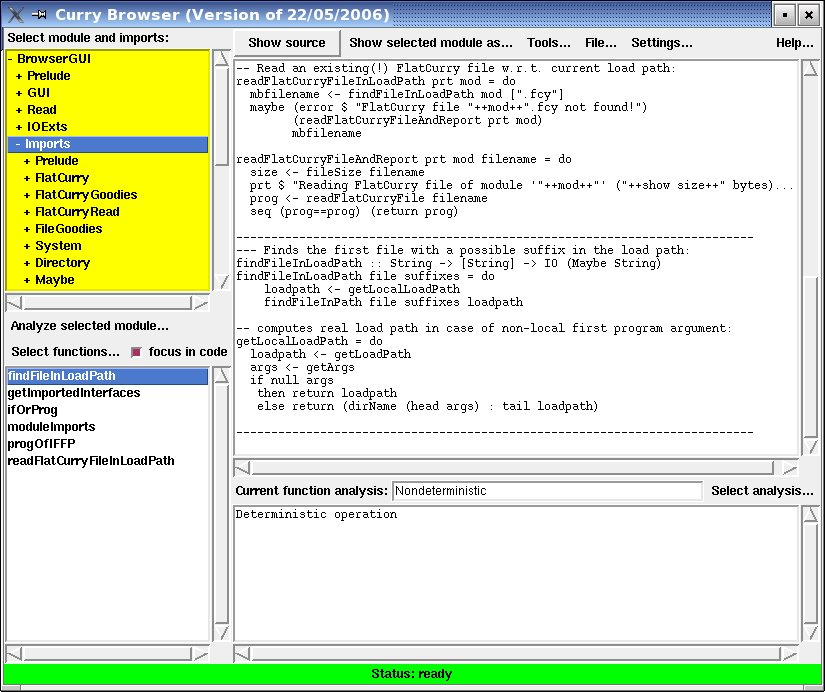
\includegraphics[scale=0.7]{currybrowser.jpg}
\end{center}
\caption{Snapshot of the main window of CurryBrowser\label{fig-currybrowser}}
\end{figure}
%
To get an impression of the use of \cb, Figure~\ref{fig-currybrowser}
shows a snapshot of its use on a particular application
(here: the implementation of \cb).
The upper list box in the left column shows the modules and their imports
in order to browse through the modules of an application.
Similarly to directory browsers, the list of imported modules of a module
can be opened or closed by clicking.
After selecting a module in the list of modules, its source code,
interface, or various other formats of the module can be shown
in the main (right) text area. For instance, one can show
pretty-printed versions of the intermediate flat programs (see below)
in order to see how local function definitions are translated by lambda lifting
\cite{Johnsson85}
or pattern matching is translated into case expressions \cite{Hanus97POPL,Wadler87}.
Since Curry is a language with parametric polymorphism and type inference,
programmers often omit the type signatures when defining functions.
Therefore, one can also view (and store) the selected module as source code where
missing type signatures are added.

Below the list box for selecting modules, there is a menu
(``Analyze selected module'') to analyze all functions
of the currently selected module at once. This is useful
to spot some functions of a module that could be problematic
in some application contexts, like functions that are impure (i.e., the result
depends on the evaluation time) or partially defined (i.e.,
not evaluable on all ground terms).
If such an analysis is selected,
the names of all functions are shown in the
lower list box of the left column (the ``function list'')
with prefixes indicating the properties of the individual functions.

The function list box can be also filled with functions
via the menu ``Select functions''. For instance, all functions
or only the exported functions defined in the currently selected
module can be shown there, or all functions from different modules
that are directly or indirectly called from
a currently selected function.
This list box is central to focus on a function in the
source code of some module or to analyze some function,
i.e., showing their properties. In order to focus on a function,
it is sufficient to check the ``focus on code'' button.
To analyze an individually selected function, one can
select an analysis from the list of available program analyses
(through the menu ``Select analysis'').
In this case, the analysis results are either shown
in the text box below the main text area
or visualized by separate tools, e.g., by a graph drawing tool for
visualizing call graphs.
Some analyses are local, i.e., they need only to consider the local definition
of this function (e.g., ``Calls directly,'' ``Overlapping rules,''
``Pattern completeness''),
where other analyses are global, i.e.,
they consider the definitions of all functions directly or indirectly called
by this function (e.g., ``Depends on,'' ``Solution complete,''
``Set-valued'').
%
Finally, there are a few additional tools integrated into \cb,
for instance, to visualize the import relation between all modules
as a dependency graph. These tools are available through the ``Tools'' menu.

More details about the use of \cb and all built-in analyses
are available through the ``Help'' menu of \cb.


\newpage

\section{CurryTest: A Tool for Testing Curry Programs}
\label{sec-currytest}

CurryTest\index{CurryTest}\index{testing programs}\index{program!testing}
is a simple tool in the PAKCS distribution to write
and run repeatable tests. CurryTest simplifies the task
of writing test cases for a module and executing them.
The tool is easy to use. Assume one has implemented a module \code{MyMod}
and wants to write some test cases to test its functionality,
making regression tests in future versions, etc.
For this purpose, there is a system library \code{Assertion}
(Section~\ref{Library:Assertion}) which
contains the necessary definitions for writing tests.
In particular, it exports an abstract polymorphic type \ccode{Assertion a}
together with the following operations:
\startprog
assertTrue      :: String -> Bool -> Assertion ()
assertEqual     :: String -> a -> a -> Assertion a
assertValues    :: String -> a -> [a] -> Assertion a
assertSolutions :: String -> (a->Success) -> [a] -> Assertion a
assertIO        :: String -> IO a -> a -> Assertion a
assertEqualIO   :: String -> IO a -> IO a -> Assertion a
\stopprog
The expression \ccode{assertTrue $s$ $b$}
is an assertion (named $s$) that the expression $b$ has the value \code{True}.
Similarly, the expression \ccode{assertEqual $s$ $e_1$ $e_2$}
asserts that the expressions $e_1$ and $e_2$
must be equal (i.e., \code{$e_1$==$e_2$} must hold),
the expression \ccode{assertValues $s$ $e$ $vs$} asserts
that $vs$ is the multiset of all values of $e$,
and the expression \ccode{assertSolutions $s$ $c$ $vs$} asserts
that the constraint abstraction $c$ has the multiset of solutions $vs$.
Furthermore, the expression \ccode{assertIO $s$ $a$ $v$}
asserts that the I/O action $a$ yields the value $v$ whenever it is
executed, and
the expression \ccode{assertEqualIO $s$ $a_1$ $a_2$}
asserts that the I/O actions $a_1$ and $a_2$ yields equal values.
The name $s$ provided as a first argument in each assertion
is used in the protocol produced by the test tool.

One can define a test program by importing the module
to be tested together with the module \code{Assertion} and defining
top-level functions of type \code{Assertion} in this module
(which must also be exported).
As an example, consider the following program
that can be used to test some list processing functions:
\startprog
\medskip
import List
import Assertion
\medskip
test1 = assertEqual     "++"     ([1,2]++[3,4]) [1,2,3,4]
\medskip
test2 = assertTrue      "all"    (all (<5) [1,2,3,4])
\medskip
test3 = assertSolutions "prefix" (\labs{}x -> let y free in  x\,++\,y =:= [1,2])
                                 [[],[1],[1,2]]
\medskip
\stopprog
For instance, \code{test1} asserts that the result of evaluating the
expression \code{([1,2]++[3,4])} is equal to \code{[1,2,3,4]}.

We can execute a test suite by the command\pindex{currytest}
\startprog
currytest testList
\stopprog
(\code{currytest} is a program stored in \code{$pakcshome$/bin}
where $pakcshome$ is the installation directory of PAKCS;
see Section~\ref{sec-general}).
In our example, \ccode{testList.curry} is the program containing the
definition of all assertions. This has the effect
that all exported top-level functions
of type \code{Assertion} are tested (i.e., the corresponding
assertions are checked) and the results
(\ccode{OK} or failure) are reported together with the name of each assertion.
%If failures occur, the complete test results are also
%written into a file named \ccode{testList.testlog}.''
For our example above, we obtain the following successful protocol:
\startprog
============================================================
Testing module "testList"...
OK: ++
OK: all
OK: prefix
All tests successfully passed.
============================================================
\stopprog
There is also a graphical interface that summarizes the results
more nicely.\footnote{Due to a bug in older versions of SICStus-Prolog,
it works only with SICStus-Prolog version 3.8.5 (or newer).}
In order to start this interface, one has to add the parameter
\ccode{--window} (or \ccode{-w}), e.g., executing a test suite by
\startprog
currytest --window testList
\stopprog
or
\startprog
currytest -w testList
\stopprog
A snapshot of the interface is shown in Figure~\ref{fig-currytest}.

\begin{figure}%[t]
\begin{center}
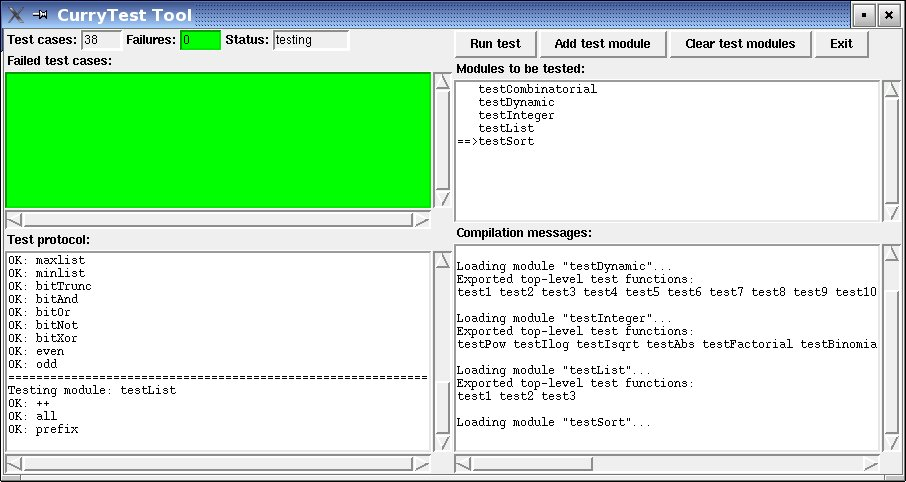
\includegraphics[scale=0.7]{currytest.jpg}
\end{center}
\caption{Snapshot of CurryTest's graphical interface\label{fig-currytest}}
\end{figure}


\newpage

\section{ERD2Curry: A Tool to Generate Programs from ER Specifications}
\label{sec-erd2curry}

ERD2Curry\index{ERD2Curry}\index{database programming}
is a tool to generate Curry code to access and manipulate data
persistently stored from
entity relationship diagrams.\index{entity relationship diagrams}
The idea of this tool is described in detail in
\cite{BrasselHanusMueller08PADL}.
Thus, we describe only the basic steps to use this tool
in the following.

If one creates an entity relationship diagram (ERD)
with the Umbrello UML Modeller, one has to store its
XML description in XMI format (as offered by Umbrello)
in a file, e.g., \ccode{myerd.xmi}.
This description can be compiled into a Curry program by the
command\pindex{erd2curry}
\startprog
erd2curry myerd.xmi
\stopprog
(\code{erd2curry} is a program stored in \code{$pakcshome$/bin}
where $pakcshome$ is the installation directory of PAKCS;
see Section~\ref{sec-general}).
If \code{MyData} is the name of the ERD, the Curry program file
\ccode{MyData.curry} is generated containing all the necessary
database access code as described in \cite{BrasselHanusMueller08PADL}.

If one does not want to use the Umbrello UML Modeller,
one can also create a textual description of the ERD
as a Curry term of type \code{ERD}
(w.r.t.\ the type definition given in module
\code{$pakcshome$/tools/erd2curry/ERD.curry})
and store it in some file, e.g., \ccode{myerd.term}.
This description can be compiled into a Curry program by the
command\pindex{erd2curry}
\startprog
erd2curry -t myerd.term
\stopprog
%
There is also the possibility to visualize an ERD term
as a graph with the graph visualization program \code{dotty}
(for this purpose, it might be necessary to adapt the definition
of the operation \code{dotCmd} in
\code{$pakcshome$/tools/erd2curry/ERD2Graph.curry}
according to your local environment).
This can be done by the command
\startprog
erd2curry -v myerd.term
\stopprog

\paragraph{Inclusion in the Curry application:}
To compile the generated database code, either
include the directory \code{$pakcshome$/tools/erd2curry}
into your Curry load path
(e.g., by setting  the environment variable
\ccode{CURRYPATH}\pindex{CURRYPATH}, see also Section~\ref{sec-modules})
or copy the file
\code{$pakcshome$/tools/erd2curry/ERDGeneric.curry}
into the directory of the generated database code.


\newpage

\section{UI: Declarative Programming of User Interfaces}
\label{sec-ui}

The PAKCS distribution contains a collection of libraries
to implement graphical user interfaces\index{user interface}
as well as web-based user interfaces
from declarative descriptions.
Exploiting these libraries, it is possible
to define the structure and functionality of a user interface
independent from the concrete technology.
Thus, a graphical user interface or a web-based user interface
can be generated from the same description by simply changing
the imported libraries.
This programming technique is described in detail in
\cite{HanusKluss09PADL}.

The libraries implementing these user interfaces are contained
in the directory
\startprog
$pakcshome$/tools/ui
\stopprog
Thus, in order to compile programs containing such user interface
specifications, one has to
include the directory \code{$pakcshome$/tools/ui}
into the Curry load path
(e.g., by setting  the environment variable
\ccode{CURRYPATH}\pindex{CURRYPATH}, see also Section~\ref{sec-modules}).
The directory
\startprog
$pakcshome$/tools/ui/examples
\stopprog
contains a few examples for such user interface specifications.


\newpage

\section{Preprocessing FlatCurry Files}
\label{sec-pakcspp}

The current parser allows to apply transformations on the intermediate
FlatCurry files after they are generated from the
corresponding Curry source file.
Currently, only the FlatCurry file corresponding to the main module
can be transformed.

A transformation can be specified as follows:
\begin{enumerate}
\item {\bf Options to \code{pakcs/bin/parsecurry}:}
\begin{description}
\item[\fbox{\code{--fpopt}}]\pindex{-fpopt}
Apply functional pattern optimization
(see \code{pakcs/tools/optimize/NonStrictOpt.curry} for details).

\item[\fbox{\code{--compact}}]\pindex{--compact}
Apply code compactification after parsing, i.e., transform the main
module and all its imported into one module and delete all
non-accessible functions.

\item[\fbox{\code{--compactexport}}]
Similar to \code{--compact} but delete all functions that are not accessible
from the exported functions of the main module.

\item[\fbox{\code{--compactmain:f}}]
Similar to \code{--compact} but delete all functions that are not accessible
from the function \ccode{f} of the main module.

\item[\fbox{\code{--fcypp cmd}}]\pindex{--fcypp}
Apply command \code{cmd} to the main module after parsing. This is useful to
integrate your own transformation into the compilation process.
Note that the command \ccode{cmd prog} should perform a transformation
on the FlatCurry file \code{prog.fcy}, i.e., it replaces the FlatCurry
file by a new one.
\end{description}

\item {\bf Setting the environment variable \code{FCYPP}:}\pindex{FCYPP}\\
For instance, setting \code{FCYPP} by
\startprog
export FCYPP="--fpopt"
\stopprog
will apply the functional pattern optimization if programs are compiled
and loaded in the PAKCS programming environment.


\item {\bf Putting options into the source code:}\pindex{PAKCS_OPTION_FCYPP}\\
If the source code contains a line with a comment of the form (the comment
must start at the beginning of the line)
\startprog
\{-\# PAKCS_OPTION_FCYPP <options> \#-\}
\stopprog
then the transformations specified by \code{<options>} are applied after
translating the source code into FlatCurry code. For instance,
the functional pattern optimization can be set by the comment
\startprog
\{-\# PAKCS_OPTION_FCYPP --fpopt \#-\}
\stopprog
in the source code. Note that this comment must be in a single line 
of the source program. If there are multiple lines containing such comments,
only the first one will be considered.
\end{enumerate}
\paragraph{Multiple options:}
Note that an arbitrary number of transformations can be specified
by the methods described above.
If several specifications for preprocessing FlatCurry files are used,
they are executed in the following order:
\begin{enumerate}
\item all transformations specified by the environemnt variable
\code{FCYPP} (from left to right)
\item all transformations specified as command line options of parsecurry
   (from left to right)
\item all transformations specified by a comment line in the source code
   (from left to right)
\end{enumerate}


\newpage

\section{Technical Problems}

Due to the fact that Curry is intended to implement
distributed systems (see Appendix~\ref{sec-ports}),
it might be possible that some technical problems
arise due to the use of sockets for implementing these
features. Therefore, this section gives some information
about the technical requirements of PAKCS and how to solve
problems due to these requirements.

There is one fixed port that is used by the implementation of PAKCS:
\begin{description}
\item[Port 8766:] This port is used by the
{\bf Curry Port Name Server} (CPNS) to implement symbolic names for
ports in Curry (see Appendix~\ref{sec-ports}).
If some other process uses this port on the machine,
the distribution facilities defined in the module \code{Ports}
(see Appendix~\ref{sec-ports}) cannot be used.
\end{description}
If these features do not work, you can try to find out
whether this port is in use by the shell command
\ccode{netstat -a | fgrep 8766} (or similar).

The CPNS is implemented as a demon listening on its port 8766
in order to serve requests about registering a new symbolic
name for a Curry port or asking the physical port number
of a Curry port. The demon will be automatically started for
the first time on a machine when a user compiles a program
using Curry ports. It can also be manually started and terminated by the
scripts \code{$pakcshome$/cpns/start} and
\code{$pakcshome$/cpns/stop}.
If the demon is already running, the command \code{$pakcshome$/cpns/start}
does nothing (so it can be always executed
before invoking a Curry program using ports).

If you detect any further technical problem,
please write to
\begin{center}
\code{mh@informatik.uni-kiel.de}
\end{center}

\newpage

\addcontentsline{toc}{section}{Bibliography}
\bibliography{manual}
\bibliographystyle{plain}

\newpage
\appendix

\section{Libraries of the PAKCS Distribution}
\label{sec:libraries}

{\setlength{\parindent}{0.0cm}

The PAKCS compiler system provides an extensive collection
of libraries for application programming.
The libraries for arithmetic constraints over real numbers,
finite domain constraints,
ports for concurrent and distributed programming, and
meta-programming by representing Curry programs in Curry
are described in the following subsection in more detail.
The complete set of libraries with all exported types and functions
are described in the further subsections.
For a more detailed online documentation of all libraries of PAKCS,
see \url{http://www.informatik.uni-kiel.de/~pakcs/lib/index.html}.

\subsection{Constraints, Ports, Meta-Programming}

\subsubsection{Arithmetic Constraints}

The primitive entities for the use of arithmetic constraints
are defined in the system module \code{CLPR}
(cf.\ Section~\ref{sec-modules}), i.e., in order to use them,
the program must contain the import declaration
\startprog
import CLPR
\stopprog
Floating point arithmetic is supported in PAKCS
via arithmetic constraints, i.e., the equational constraint
\ccode{2.3 +.~x =:= 5.5} is solved by binding \code{x} to \code{3.2}
(rather than suspending the evaluation of the addition,
as in corresponding constraints on integers like
\ccode{3+x=:=5}). All operations related to
floating point numbers are suffixed by \ccode{.}.
The following functions and constraints on floating point
numbers are supported in PAKCS:
\begin{description}
\item[\code{(+.)   :: Float -> Float -> Float}]~\\
Addition on floating point numbers.
\item[\code{(-.)   :: Float -> Float -> Float}]~\\
Subtraction on floating point numbers.
\item[\code{(*.)   :: Float -> Float -> Float}]~\\
Multiplication on floating point numbers.
\item[\code{(/.)   :: Float -> Float -> Float}]~\\
Division on floating point numbers.
\item[\code{(<.)   :: Float -> Float -> Success}]~\\
Comparing two floating point numbers with the ``less than'' relation.
\item[\code{(>.)   :: Float -> Float -> Success}]~\\
Comparing two floating point numbers with the ``greater than'' relation.
\item[\code{(<=.)  :: Float -> Float -> Success}]~\\
Comparing two floating point numbers with the ``less than or equal'' relation.
\item[\code{(>=.)  :: Float -> Float -> Success}]~\\
Comparing two floating point numbers with the ``greater than or equal''
relation.
\item[\code{i2f    :: Int -> Float}]~\\
Converting an integer number into a floating point number.
\end{description}
As an example, consider a constraint \code{mortgage}
which relates the principal \code{p},
the lifetime of the mortgage in months \code{t},
the monthly interest rate \code{ir},
the monthly repayment \code{r},
and the outstanding balance at the end of the lifetime \code{b}.
The financial calculations
can be defined by the following two rules in Curry (the second rule
describes the repeated accumulation of the interest):
\startprog
~
import CLPR
~
mortgage p t ir r b | t >. 0.0 \& t <=. 1.0  --lifetime not more than 1 month?
                    =  b =:= p *. (1.0 +. t *. ir) -. t*.r \vspace{1ex}
mortgage p t ir r b | t >. 1.0               --lifetime more than 1 month?
                    =  mortgage (p *. (1.0+.ir)-.r) (t-.1.0) ir r b
~
\stopprog
Then we can calculate the monthly payment for paying back
a loan of \$100,000 in 15 years with a monthly interest rate of 1\%
by solving the goal
\startprog
mortgage 100000.0 180.0 0.01 r 0.0
\stopprog
which yields the solution \code{r=1200.17}.

Note that only linear arithmetic equalities or inequalities
are solved by the constraint solver. Non-linear constraints
like \ccode{x *.~x =:= 4.0} are suspended until they become
linear.


\subsubsection{Finite Domain Constraints}

Finite domain constraints are constraints where all variables
can only take a finite number of possible values.
For simplicity, the domain of finite domain variables are
identified with a subset of the integers, i.e., the type
of a finite domain variable is \code{Int}. The arithmetic
operations related to finite domain variables are suffixed by \ccode{\#}.
The following functions and constraints for finite domain constraint solving
are currently supported in PAKCS:\footnote{Note that
this library is based on the corresponding library of SICStus-Prolog
but does not implement the complete functionality of the SICStus-Prolog library.
However, using the PAKCS interface for external functions (see
Appendix~\ref{sec-external-functions}), it is relatively
easy to provide the complete functionality.}

\begin{description}
\item[\code{domain :: [Int] -> Int -> Int -> Success}]~\\
The constraint \ccode{domain [$x_1,\ldots,x_n$] $l$ $u$}
is satisfied if the domain of all variables $x_i$ is the interval $[l,u]$.
\item[\code{(+\#)   :: Int -> Int -> Int}]~\\
Addition on finite domain values.
\item[\code{(-\#)   :: Int -> Int -> Int}]~\\
Subtraction on finite domain values.
\item[\code{(*\#)   :: Int -> Int -> Int}]~\\
Multiplication on finite domain values.
\item[\code{(=\#)   :: Int -> Int -> Success}]~\\
Equality of finite domain values.
\item[\code{(/=\#)  :: Int -> Int -> Success}]~\\
Disequality of finite domain values.
\item[\code{(<\#)   :: Int -> Int -> Success}]~\\
``less than'' relation on finite domain values.
\item[\code{(<=\#)  :: Int -> Int -> Success}]~\\
``less than or equal'' relation on finite domain values.
\item[\code{(>\#)   :: Int -> Int -> Success}]~\\
``greater than'' relation on finite domain values.
\item[\code{(>=\#)  :: Int -> Int -> Success}]~\\
``greater than or equal'' relation on finite domain values.
\item[\code{sum :: [Int] -> (Int -> Int -> Success) -> Int -> Success}]~\\
The constraint \ccode{sum [$x_1,\ldots,x_n$] $op$ $x$}
is satisfied if all $x_1+\cdots + x_n \mathrel{op} x$ is satisfied,
where $op$ is one of the above finite domain constraint relations
(e.g., \ccode{=\#}).
\item[\code{scalar_product :: [Int] -> [Int] -> (Int -> Int -> Success) -> Int -> Success}]~\\
The constraint \ccode{scalar_product [$c_1,\ldots,c_n$] [$x_1,\ldots,x_n$] $op$ $x$}
is satisfied if all $c_1 x_1+\cdots + c_n x_n \mathrel{op} x$ is satisfied,
where $op$ is one of the above finite domain constraint relations.
\item[\code{count :: Int -> [Int] -> (Int -> Int -> Success) -> Int -> Success}]~\\
The constraint \ccode{count $k$ [$x_1,\ldots,x_n$] $op$ $x$}
is satisfied if all $k \mathrel{op} x$ is satisfied,
where $n$ is the number of the $x_i$ that are equal to $k$ and
$op$ is one of the above finite domain constraint relations.
\item[\code{all_different :: [Int] -> Success}]~\\
The constraint \ccode{all_different [$x_1,\ldots,x_n$]}
is satisfied if all $x_i$ have pairwise different values.
\item[\code{labeling :: [LabelingOption] -> [Int] -> Success}]~\\
The constraint \ccode{labeling $os$ [$x_1,\ldots,x_n$]}
non-deterministically instantiates all $x_i$ to the values
of their domain according to the options $os$ (see the module documentation
for further details about these options).
\end{description}
These entities are defined in the system module \code{CLPFD}
(cf.\ Section~\ref{sec-modules}), i.e., in order to use it,
the program must contain the import declaration
\startprog
import CLPFD
\stopprog
As an example, consider the classical \ccode{send+more=money} problem
where each letter must be replaced by a different digit such that this
equation is valid and there are no leading zeros.
The usual way to solve finite domain constraint problems
is to specify the domain of the involved variables followed
by a specification of the constraints and the labeling
of the constraint variables in order to start the search for solutions.
Thus, the \ccode{send+more=money} problem can be solved as follows:
\startprog
~
import CLPFD
~
smm l =
        l =:= [s,e,n,d,m,o,r,y] \&
        domain l 0 9 \&
        s >\# 0 \&
        m >\# 0 \&
        all_different l  \&
                         1000 *\# s +\# 100 *\# e +\# 10 *\# n +\# d
        +\#               1000 *\# m +\# 100 *\# o +\# 10 *\# r +\# e
        =\# 10000 *\# m +\# 1000 *\# o +\# 100 *\# n +\# 10 *\# e +\# y \&
        labeling [FirstFail] l
        where s,e,n,d,m,o,r,y free
~
\stopprog
Then we can solve this problem by evaluating the goal
\ccode{smm [s,e,n,d,m,o,r,y]} which yields the unique solution
\code{\{s=9,e=5,n=6,d=7,m=1,o=0,r=8,y=2\}}.


\subsubsection{Ports: Distributed Programming in Curry}
\label{sec-ports}

To support the development of concurrent and distributed applications,
PAKCS supports internal and external ports\index{ports} as
described in \cite{Hanus99PPDP}.
Since \cite{Hanus99PPDP} contains a detailed description of this
concept together with various programming examples, we only summarize here
the functions and constraints supported for ports in PAKCS.

The basic datatypes, functions, and constraints for ports
are defined in the system module \code{Ports}
(cf.\ Section~\ref{sec-modules}), i.e., in order to use ports,
the program must contain the import declaration
\startprog
import Ports
\stopprog
This declaration includes the following entities in the program:
\begin{description}
\item[\code{Port a}\pindex{Port}]~\\
This is the datatype of a port to which one can send messages of type \code{a}.

\item[\code{openPort :: Port a -> [a] -> Success}]~\\
The constraint \ccode{openPort p s}\pindex{openPort}
establishes a new \emph{internal port}
\code{p} with an associated message stream \code{s}. \code{p} and \code{s} must be
unbound variables,
otherwise the constraint fails (and causes a runtime error).

\item[\code{send :: a -> Port a -> Success}]~\\
The constraint \ccode{send m p}\pindex{send}
is satisfied if \code{p} is constrained
to contain the message \code{m}, i.e., \code{m} will be sent to the port
\code{p} so that it appears in the corresponding stream.

\item[\code{doSend :: a -> Port a -> IO ()}]~\\
The I/O action \ccode{doSend m p}\pindex{doSend} solves the constraint
\ccode{send m p} and returns nothing.

\item[\code{openNamedPort :: String -> IO [a]}]~\\
The I/O action \ccode{openNamedPort n}\pindex{openNamedPort}
opens a new \emph{external port} with
symbolic name \code{n} and returns the associated stream of messages.

\item[\code{connectPort :: String -> IO (Port a)}]~\\
The I/O action \ccode{connectPort n}\pindex{connectPort}
returns a port with symbolic name
\code{n} (i.e., \code{n} must have the form ``\emph{portname@machine})
to which one can send messages by the \code{send} constraint.
Currently, no dynamic type checking is done for external ports,
i.e., sending messages of the wrong type to a port might lead to
a failure of the receiver.
\end{description}

\paragraph{Restrictions:}
Every expression, possibly containing logical variables, can be sent to
a port. However, as discussed in \cite{Hanus99PPDP},
port communication is strict, i.e., the expression is
evaluated to normal form before sending it by the
constraint \code{send}. Furthermore, if messages containing
logical variables are sent to \emph{external ports},
the behavior is as follows:
\begin{enumerate}
\item The sender waits until all logical variables in the message
have been bound by the receiver.
\item The binding of a logical variable received by a process
is sent back to the sender of this logical variable only if
it is bound to a \emph{ground} term, i.e., as long as the binding contains
logical variables, the sender is not informed about the binding
and, therefore, the sender waits.
\end{enumerate}

\paragraph{External ports on local machines:}
The implementation of external ports assumes that the
host machine running the application is connected to the Internet
(i.e., it uses the standard IP address of the host machine
for message sending). If this is not the case and the application
should be tested by using external ports only on the local host
without a connection to the Internet,
the environment variable \ccode{PAKCS_LOCALHOST}\pindex{PAKCS_LOCALHOST}
must be set to \ccode{yes}
\emph{before PAKCS system is started}.
In this case, the IP address \code{127.0.0.1} and the hostname
\ccode{localhost} are used for identifying the local machine.

\paragraph{Selection of Unix sockets for external ports:}
The implementation of ports uses sockets to communicate
messages sent to external ports.
Thus, if a Curry program uses the
I/O action \code{openNamedPort}\pindex{openNamedPort}
to establish an externally visible server,
PAKCS selects a Unix socket for the port communication.
Usually, a free socket is selected by the operating system.
If the socket number should be fixed in an application (e.g.,
because of the use of firewalls\index{firewall} that allow only
communication over particular sockets), then one
can set the environment variable \ccode{PAKCS_SOCKET}\pindex{PAKCS_SOCKET}
to a distinguished socket number before the PAKCS system is started.
This has the effect that PAKCS uses only this socket
number for communication (even for several external ports
used in the same application program).

\paragraph{Debugging:}
To debug distributed systems,
it is sometimes helpful to see all messages sent to external ports.
This is supported by the environment variable
\ccode{PAKCS_TRACEPORTS}.\pindex{PAKCS_TRACEPORTS}
If this variable is set to \ccode{yes}
\emph{before the PAKCS system is started}, then all
connections to external ports and all
messages sent and received on external ports are
printed on the standard error stream.


\subsubsection{AbstractCurry and FlatCurry: Meta-Programming in Curry}
\label{sec-flatcurry}

\index{AbstractCurry}
\index{FlatCurry}
To support meta-programming, i.e., the manipulation of Curry programs
in Curry, there are system modules \code{FlatCurry} and \code{AbstractCurry}
(stored in the directory \ccode{$pakcshome$/lib/meta})
which define datatypes for the representation
of Curry programs.
\code{AbstractCurry} is a more direct representation of a Curry program,
whereas \code{FlatCurry} is a simplified representation
where local function definitions are replaced by global definitions
(i.e., lambda lifting has been performed) and pattern matching
is translated into explicit case/or expressions.
Thus, \code{FlatCurry} can be used for more back-end oriented
program manipulations (or, for writing new back ends for Curry),
whereas \code{AbstractCurry} is intended for manipulations of
programs that are more oriented towards the source program.

Both modules contain predefined I/O actions to read programs
in the \code{AbstractCurry} (\code{readCurry}\pindex{readCurry})
or \code{FlatCurry}
(\code{readFlatCurry}\pindex{readFlatCurry}) format.
These actions parse the corresponding source program and return
a data term representing this program (according to the definitions
in the modules \code{AbstractCurry} and \code{FlatCurry}).

Since all datatypes are explained in detail in these modules,
we refer to the online documentation\footnote{%
\url{http://www.informatik.uni-kiel.de/~pakcs/lib/CDOC/FlatCurry.html} and
\url{http://www.informatik.uni-kiel.de/~pakcs/lib/CDOC/AbstractCurry.html}}
of these modules.

As an example, consider a program file \ccode{test.curry}
containing the following two lines:
\startprog
rev []     = []
rev (x:xs) = (rev xs) ++ [x]
\stopprog
Then the I/O action \code{(FlatCurry.readFlatCurry "test")} returns the
following term:
\startprog
 (Prog "test"
  ["Prelude"]
  []
  [Func ("test","rev") 1 Public
        (FuncType (TCons ("Prelude","[]") [(TVar 0)])
                  (TCons ("Prelude","[]") [(TVar 0)]))
        (Rule [0]
           (Case Flex (Var 0)
              [Branch (Pattern ("Prelude","[]") [])
                  (Comb ConsCall ("Prelude","[]") []),
               Branch (Pattern ("Prelude",":") [1,2])
                  (Comb FuncCall ("Prelude","++")
                        [Comb FuncCall ("test","rev") [Var 2],
                         Comb ConsCall ("Prelude",":")
                              [Var 1,Comb ConsCall ("Prelude","[]") []]
                        ])
              ]))]
  []
 )
\stopprog


%%%%%%%%%%%%%%%%%%%%%%%%%%%%%%%%%%%%%%%%%%%%%%%%%%%%%%%%%%%%%%%%%%%%%%%%%
% Definitions in order to LaTeX documents generated by "currydoc --tex"
%%%%%%%%%%%%%%%%%%%%%%%%%%%%%%%%%%%%%%%%%%%%%%%%%%%%%%%%%%%%%%%%%%%%%%%%%

\newcommand{\currymodule}[1]{\subsubsection{Library #1}\label{Library:#1}}
\newcommand{\currytypesstart}{\subsubsection*{Exported types:}}
\newcommand{\currytypesstop}{}
\newcommand{\currytypesynstart}[2]{{\tt type #2}\pindex{#1} \begin{quote}}
\newcommand{\currytypesynstop}{\end{quote}}
\newcommand{\currydatastart}[1]{{\tt data #1}\pindex{#1} \begin{quote}}
\newcommand{\currydatacons}{\end{quote}%
\begin{itemize}\item[] \hspace{-4ex}\emph{Exported constructors:}}
\newcommand{\currydatastop}{\end{itemize}}
\newcommand{\curryconsstart}[2]{\item {\tt #1~::~#2}\par}
\newcommand{\curryfuncstart}{\subsubsection*{Exported functions:}}
\newcommand{\curryfuncstop}{}
\newcommand{\curryfunctionstart}[2]{#2\pindex{#1}\begin{quote}}
\newcommand{\curryfunctionstop}{\end{quote}}
\newcommand{\curryfuncsig}[2]{{\tt #1~::~#2}}


\subsection{General Libraries}

\input{lib/AllSolutions}
\input{lib/Assertion}
\input{lib/Char}
\input{lib/CLPFD}
\input{lib/CLPR}
\input{lib/CLPB}
\input{lib/Combinatorial}
\input{lib/Constraint}
\input{lib/CSV}
\input{lib/Database}
\input{lib/DaVinci}
\input{lib/Directory}
\input{lib/Dynamic}
\input{lib/FileGoodies}
\input{lib/Float}
\input{lib/Global}
\input{lib/GlobalVariable}
\input{lib/GUI}
\input{lib/Integer}
\input{lib/IO}
\input{lib/IOExts}
\input{lib/JavaScript}
\input{lib/KeyDatabase}
\input{lib/KeyDatabaseSQLite}
\input{lib/KeyDB}
\input{lib/List}
\input{lib/Maybe}
\input{lib/NamedSocket}
\input{lib/Parser}
\input{lib/Ports}
\input{lib/Pretty}
\input{lib/Profile}
\input{lib/PropertyFile}
\input{lib/Read}
\input{lib/ReadNumeric}
\input{lib/ReadShowTerm}
\input{lib/SetFunctions}
\input{lib/Socket}
\input{lib/System}
\input{lib/Time}
%\input{lib/Tk}
\input{lib/Unsafe}


\subsection{Data Structures and Algorithms}

\input{lib/Array}
\input{lib/Dequeue}
\input{lib/FiniteMap}
\input{lib/GraphInductive}
\input{lib/Random}
\input{lib/RedBlackTree}
\input{lib/SetRBT}
\input{lib/Sort}
\input{lib/TableRBT}
\input{lib/Traversal}

\subsection{Libraries for Web Applications}

\input{lib/CategorizedHtmlList}
\input{lib/HTML}
\input{lib/HtmlParser}
\input{lib/Mail}
\input{lib/Markdown}
\input{lib/WUI}
\input{lib/URL}
\input{lib/XML}
\input{lib/XmlConv}

\subsection{Libraries for Meta-Programming}

\input{lib/AbstractCurry}
\input{lib/AbstractCurryPrinter}
\input{lib/CompactFlatCurry}
\input{lib/CurryStringClassifier}
\input{lib/FlatCurry}
\input{lib/FlatCurryGoodies}
\input{lib/FlatCurryRead}
\input{lib/FlatCurryShow}
\input{lib/FlatCurryTools}
\input{lib/FlatCurryXML}
\input{lib/FlexRigid}
\input{lib/PrettyAbstract}

} % end setlength parindent

\newpage

\input{markdown_syntax}

\newpage

\begin{figure}%[t]
\begin{center}
 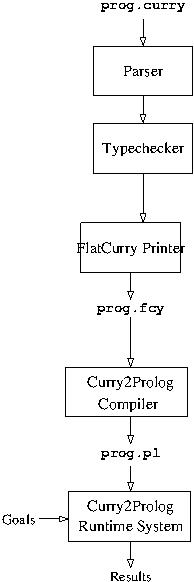
\includegraphics[scale=0.85]{pakcs_overview.jpg}
\end{center}\vspace{-5ex}
\caption{Overview of PAKCS\label{fig-pakcs}}
\end{figure}

\section{Overview of the PAKCS Distribution}

A schematic overview of the various components contained in
the distribution of PAKCS and the
translation process of programs inside PAKCS is shown in
Figure~\ref{fig-pakcs} on page~\pageref{fig-pakcs}.
In this figure, boxes denote different components of PAKCS
and names in boldface denote files containing
various intermediate representations during the translation
process (see Section~\ref{sec-auxfiles} below).
The PAKCS distribution contains a front end for reading (parsing and
type checking) Curry programs that can be also used by
other Curry implementations.
The back end (formerly known as ``Curry2Prolog''\index{Curry2Prolog})
compiles Curry programs into Prolog programs.
It also support constraint solvers for
arithmetic constraints over real numbers and finite domain constraints,
and further libraries for GUI programming, meta-programming etc.
Currently, it does not implement encapsulated search in full generality
(only a strict version of \code{findall} is supported),
and concurrent threads are not executed in a fair manner.


\newpage

\section{Auxiliary Files}
\label{sec-auxfiles}

During the translation and execution of a Curry program with PAKCS,
various intermediate representations of the source program are created
and stored in different files which are shortly explained in this section.
If you use the PAKCS, it is not necessary to know about
these auxiliary files because they are automatically generated
and updated. You should only remember the command for deleting
all auxiliary files (\ccode{cleancurry}, see Section~\ref{sec-general})
to clean up your directories.

The various components of PAKCS create
the following auxiliary files.
\begin{description}
\item[\code{prog.fcy}:] This file contains the Curry program
in the so-called ``FlatCurry'' representation where all functions are global
(i.e., lambda lifting has been performed) and pattern matching
is translated into explicit case/or expressions
(compare Appendix~\ref{sec-flatcurry}).
This representation might be useful for other back ends and
compilers for Curry and is the basis doing meta-programming in Curry.
This file is implicitly
generated when a program is read by PAKCS.
It can be also explicitly generated by the command\pindex{parsecurry}
\startprog
parsecurry --flat prog
\stopprog
The FlatCurry representation of a Curry program is usually
generated by the front-end after parsing, type checking and eliminating
local declarations.
If $dir$ is the directory where the Curry program is stored,
the corresponding FlatCurry program is stored in the directory
\ccode{$dir$/.curry}.

\item[\code{prog.fint}:] This file contains the interface
of the program in the so-called ``FlatCurry'' representation,
i.e., it is similar to \code{prog.fcy} but contains only exported
entities and the bodies of all functions omitted (i.e., ``external'').
This representation is useful for providing a fast access
to module interfaces.
This file is implicitly generated by the command\pindex{parsecurry}
\startprog
parsecurry --flat prog
\stopprog
and stored in the same directory as \code{prog.fcy}.

\item[\code{prog.pl}:] This file contains a Prolog program
as the result of translating the Curry program with PAKCS.
If $dir$ is the directory where the Curry program is stored,
the corresponding Prolog program is stored in the directory
\ccode{$dir$/.curry/.pakcs}.

\item[\code{prog.po}:] This file contains the Prolog program
\code{prog.pl} in an intermediate format for faster loading.
This file is stored in the same directory as \code{prog.pl}.

\item[\code{prog.state}:] This file contains the saved state
after compiling and saving a program with PAKCS
(see Section~\ref{sec-use-curry2prolog}).

\end{description}


\newpage


\section{Changing the Prelude or System Modules}

The standard prelude, which is automatically imported into each Curry program,
and all system modules containing datatypes and functions
useful for application programming
(cf.\ Appendix~\ref{sec:libraries})
are stored in the system module directory \ccode{$pakcshome$/lib}
(and its subdirectories).
If you change any of these modules,
you have to recompile the complete system by
executing \code{make} in the directory $pakcshome$.



\newpage

\section{External Functions}
\label{sec-external-functions}

\index{function!external}\index{external function}
Currently, PAKCS has no general interface to external functions.
Therefore, if a new external function should be added
to the system, this function must be declared as \code{external}
in the Curry source code
and then an implementation for this external function
must be inserted in the corresponding back end.
An external function is defined as follows in the Curry source code:
\begin{enumerate}
\item
Add a type declaration for the external function somewhere
in the body of the appropriate file (usually, the prelude
or some system module).
\item
For external functions it is not allowed to define any
rule since their semantics is determined by an external implementation.
Instead of the defining rules, you have to write
\startprog
f external
\stopprog
somewhere in the file containing the type declaration for 
the external function \code{f}.
\end{enumerate}
For instance, the addition on integers can be declared as
an external function as follows:
\startprog
(+) :: Int -> Int -> Int
(+) external
\stopprog
The further modifications to be done for an inclusion of
an external function has to be done in the back end.
A new external function is added to the back end of PAKCS
by informing the compiler about the existence of an external function
and adding an implementation of this function in the run-time
system. Therefore, the following items must be added
in the PAKCS compiler system:
\begin{enumerate}
\item
If the Curry module \code{Mod} contains external functions,
there must be a file named \code{Mod.prim_c2p} containing the
specification of these external functions. The contents of this file
is in XML format and has the following general structure:\footnote{%
\url{http://www.informatik.uni-kiel.de/~pakcs/primitives.dtd} contains a DTD
describing the exact structure of these files.}
\startprog
<primitives>
  \emph{specification of external function $f_1$}
  \ldots
  \emph{specification of external function $f_n$}
</primitives>
\stopprog
The specification of an external function $f$
with arity $n$ has the form
\startprog
<primitive name="$f$" arity="$n$">
  <library>lib</library>
  <entry>pred</entry>
</primitive>
\stopprog
where \code{lib} is the Prolog library (stored in the directory of the
Curry module or in the global directory
\code{$pakcshome$/curry2prolog/lib_src}) containing the code implementing this
function and \code{pred} is a predicate name in this library
implementing this function. Note that the function $f$ must be
declared in module \code{Mod}: either as an external function
or defined in Curry by equations. In the latter case,
the Curry definition is not translated but calls to this function
are redirected to the Prolog code specified above.

Furthermore, the list of specifications can also contain entries of the form
\startprog
<ignore name="$f$" arity="$n$" />
\stopprog
for functions $f$ with arity $n$ that are declared in module \code{Mod}
but should be ignored for code generation, e.g., since they are
never called w.r.t.\ to the current implementation of external functions.
For instance, this is useful when functions that can
be defined in Curry should be (usually more efficiently) are implemented
as external functions.

Note that the arguments are passed in their current (possibly unevaluated) form.
Thus, if the external function requires the arguments to be evaluated
in a particular form, this must be done before calling the external function.
For instance, the external function for adding two integers
requires that both arguments must be evaluated to non-variable head normal form
(which is identical to the ground constructor normal form). Therefore,
the function \ccode{+} is specified in the prelude by
\startprog
(+)   :: Int -> Int -> Int
x + y = (prim_Int_plus \$\# y) \$\# x
\medskip
prim_Int_plus :: Int -> Int -> Int
prim_Int_plus external
\stopprog
where \code{prim_Int_plus} is the actual external function implementing
the addition on integers. Consequently, the specification file
\code{Prelude.prim_c2p} has an entry of the form
\startprog
<primitive name="prim_Int_plus" arity="2">
  <library>prim_standard</library>
  <entry>prim_Int_plus</entry>
</primitive>
\stopprog
where the Prolog library \code{prim_standard.pl} contains the Prolog code
implementing this function.

\item
For most external functions, a \emph{standard interface} is
generated by the compiler so that an $n$-ary function can be
implemented by an $(n+1)$-ary predicate where the last argument must
be instantiated to the result of evaluating the function.  The
standard interface can be used if all arguments are ensured to be
fully evaluated (e.g., see definition of \code{(+)} above) and no
suspension control is necessary, i.e., it is ensured that the
external function call does not suspend for all arguments.
Otherwise, the raw interface (see below) must be used.  For
instance, the Prolog code implementing \code{prim_Int_plus}
contained in the Prolog library \code{prim_standard.pl} is as
follows (note that the arguments of \code{(+)} are passed in reverse
order to \code{prim_Int_plus} in order to ensure a left-to-right
evaluation of the original arguments by the calls to \code{(\$\#)}):
\startprog
prim_Int_plus(Y,X,R) :- R is X+Y.
\stopprog

\item
The \emph{standard interface for I/O actions}, i.e., external functions
with result type \code{IO~a}, assumes that the I/O action
is implemented as a predicate (with a possible side effect)
that instantiates the last argument to the returned value of type \ccode{a}.
For instance, the primitive predicate \code{prim_getChar}
implementing prelude I/O action \code{getChar}
can be implemented by the Prolog code
\startprog
prim_getChar(C) :- get_code(N), char_int(C,N).
\stopprog
where \code{char_int} is a predicate relating the internal
Curry representation of a character with its ASCII value.

\item
If some arguments passed to the external functions are not fully evaluated
or the external function might suspend, the implementation must follow
the structure of the PAKCS run-time system by using
the \emph{raw interface}. In this case, the name of the external entry
must be suffixed by \ccode{[raw]} in the \code{prim_c2p} file.
For instance, if we want to use the raw interface for the external function
\code{prim_Int_plus},
the specification file \code{Prelude.prim_c2p} must have an entry of the form
\startprog
<primitive name="prim_Int_plus" arity="2">
  <library>prim_standard</library>
  <entry>prim_Int_plus[raw]</entry>
</primitive>
\stopprog
In the raw interface, the actual implementation of an $n$-ary external function consists
of the definition of an $(n+3)$-ary predicate $pred$.
The first $n$ arguments are the corresponding actual arguments.
The $(n+1)$-th argument is a free variable which must be
instantiated to the result of the function call after
successful execution. The last two arguments
control the suspension behavior of the function
(see \cite{AntoyHanus00FROCOS} for more details):
The code for the predicate $pred$
should only be executed when the $(n+2)$-th argument
is not free, i.e., this predicate has always the
SICStus-Prolog block declaration
\startprog
?- block $pred$(?,\ldots,?,-,?).
\stopprog
In addition, typical external functions should suspend
until the actual arguments are instantiated. This can be ensured
by a call to \code{ensureNotFree} or \code{(\$\#)}
before calling the external function. Finally, the
last argument (which is a free variable at call time)
must be unified with the $(n+2)$-th argument
after the function call is successfully evaluated
(and does not suspend). Additionally, the actual (evaluated) arguments
must be dereferenced before they are accessed.
Thus, an implementation
of the external function for adding integers is as follows in the raw interface:
\startprog
?- block prim_Int_plus(?,?,?,-,?).
prim_Int_plus(RY,RX,Result,E0,E) :-
     deref(RX,X), deref(RY,Y), Result is X+Y, E0=E.
\stopprog
Here, \code{deref} is a predefined predicate for dereferencing the
actual argument into a constant (and \code{derefAll} for dereferencing
complex structures).
\end{enumerate}
%
The Prolog code implementing the external functions must be accessible to the run-time
system of PAKCS by putting it into the directory containing the corresponding
Curry module or into the system directory
\code{$pakcshome$/curry2prolog/lib_src}.
Then it will be automatically loaded into the run-time environment
of each compiled Curry program.

Note that arbitrary functions implemented in C or Java can be connected to
PAKCS by using the corresponding interfaces of underlying Prolog system.


\newpage
\addcontentsline{toc}{section}{Index}
\printindex


\end{document}

\clearpage
\documentclass[11pt,fleqn]{article}

\usepackage{latexsym}
\usepackage{makeidx}
\usepackage{url}
\usepackage{xspace}
\usepackage{graphicx}

\input{version}

%%% ------------------------------------------------------------------

\usepackage[colorlinks,linkcolor=blue]{hyperref}
\hypersetup{bookmarksopen=true}
\hypersetup{bookmarksopenlevel=0}
\hypersetup{pdftitle={PAKCS: The Portland Aachen Kiel Curry System}}
\hypersetup{pdfauthor={Michael Hanus}}
%\hypersetup{pdfstartview=Title}
\hypersetup{pdfstartview=FitH}
\usepackage{thumbpdf}

%%% ------------------------------------------------------------------

\setlength{\textwidth}{16.5cm}
\setlength{\textheight}{23cm}
\renewcommand{\baselinestretch}{1.1}
\setlength{\topmargin}{-1cm}
\setlength{\oddsidemargin}{0cm}
\setlength{\evensidemargin}{0cm}
\setlength{\marginparwidth}{0.0cm}
\setlength{\marginparsep}{0.0cm}

\newlength{\figurewidth}
\setlength{\figurewidth}{\textwidth}
\addtolength{\figurewidth}{-0.4cm}

% font for program texts
\renewcommand{\tt}{\usefont{OT1}{cmtt}{m}{n}\selectfont}
\newcommand{\codefont}{\tt}

% environment for typing program texts:
\makeatletter
\newenvironment{prog}{\par\vspace{0.7ex}
\setlength{\parindent}{1.0cm}
\setlength{\parskip}{-0.1ex}
\obeylines\@vobeyspaces\tt}{\vspace{0.7ex}\noindent
}
\makeatother
\newcommand{\startprog}{\begin{prog}}
\newcommand{\stopprog}{\end{prog}\noindent}

% program text in normal text
\newcommand{\code}[1]{\mbox{\codefont #1}}

% program text in normal text with apostrophs
\newcommand{\ccode}[1]{``\mbox{\codefont #1}''}

\newcommand{\pindex}[1]{\index{#1@{\tt #1}}}  % program elements in index

\newcommand{\labs}{\mbox{\tt\char92}}  % lambda abstraction in Curry
\newcommand{\todo}[1]{\fbox{\sc To do: #1}}
\newcommand{\cb}{CurryBrowser\xspace}

% allow underscores in programs:
\catcode`\_=\active
\let_=\sb
\catcode`\_=12

% produce an index:
\makeindex

\begin{document}
\sloppy

\begin{titlepage}
\pdfbookmark[1]{Title}{Title}
\begin{center}
\fbox{
\begin{minipage}[t]{\figurewidth}
\begin{center}\vspace{10ex}
{\Huge\bf PAKCS \pakcsversion}\\[4ex]
{\huge The Portland Aachen Kiel Curry System}\\[7ex]
{\huge User Manual}\\[4ex]
\pakcsversiondate\\[6ex]
\Large
Michael Hanus$^1$ [editor] \\[3ex]
{\large Additional Contributors:}\\[2ex]
Sergio Antoy$^2$ \\
Bernd Bra\ss{}el$^3$ \\
Martin Engelke$^4$ \\
Klaus H\"oppner$^5$ \\
Johannes Koj$^6$ \\
Philipp Niederau$^7$ \\
Ramin Sadre$^8$ \\
Frank Steiner$^9$ \\[4ex]
\normalsize
(1) University of Kiel, Germany, {\tt mh@informatik.uni-kiel.de} \\
(2) Portland State University, USA, {\tt antoy@cs.pdx.edu} \\
(3) University of Kiel, Germany, {\tt bbr@informatik.uni-kiel.de} \\
(4) University of Kiel, Germany, {\tt men@informatik.uni-kiel.de} \\
(5) University of Kiel, Germany, {\tt klh@informatik.uni-kiel.de} \\
(6) RWTH Aachen, Germany, {\tt johannes.koj@sdm.de} \\
(7) RWTH Aachen, Germany, {\tt philipp@navigium.de} \\
(8) RWTH Aachen, Germany, {\tt ramin@lvs.informatik.rwth-aachen.de} \\
(9) LMU Munich, Germany, {\tt fst@bio.informatik.uni-muenchen.de} \\[5ex]~
\end{center}
\end{minipage}}
\end{center}
\end{titlepage}

\pdfbookmark[1]{Contents}{Contents}
\tableofcontents

\newpage

\addcontentsline{toc}{section}{Preface}
\section*{Preface}

This document describes PAKCS (formerly called ``PACS''),
an implementation of the multi-paradigm language Curry,
jointly developed at the University of Kiel, the Technical University
of Aachen and Portland State University.
Curry is a universal programming language aiming at the amalgamation
of the most important declarative programming paradigms,
namely functional programming and logic programming.  
Curry combines in a seamless way features from functional programming
(nested expressions, lazy evaluation, higher-order functions),
logic programming (logical variables, partial data structures,
built-in search), and concurrent programming (concurrent evaluation
of constraints with synchronization on logical variables).
Moreover, the PAKCS implementation of Curry also supports
the high-level implementation of distributed applications,
graphical user interfaces, and web services
(as described in more detail in \cite{Hanus99PPDP,Hanus00PADL,Hanus01PADL}).

We assume familiarity with the ideas and features
of Curry as described in the Curry language definition \cite{Hanus12Curry}.
Therefore, this document only explains the use of the different
components of PAKCS
and the differences and restrictions of PAKCS
(see Section~\ref{sec-restrictions})
compared with the language Curry (Version 0.8.3).


\bigskip

\subsection*{Acknowledgements}

This work has been supported in part by the DAAD/NSF grant INT-9981317,
the NSF grants CCR-0110496 and CCR-0218224,
the Acci\'on Integrada hispano-alemana HA1997-0073,
and the DFG grants Ha 2457/1-2, Ha 2457/5-1, and Ha 2457/5-2.

Many thanks to the users of PAKCS for bug reports, bug fixes, and improvements,
in particular, to Marco Comini, Sebastian Fischer, Massimo Forni,
Carsten Heine, Stefan Junge, Frank Huch, Parissa Sadeghi.


\newpage

\section{Overview of PAKCS}

\subsection{General Use}
\label{sec-general}

This version of PAKCS has been tested on Sun Solaris, Linux, and Mac OS X
systems. In principle, it should be also executable on other
platforms on which a Prolog system like SICStus-Prolog or SWI-Prolog exists
(see the file \code{INSTALL.html} in the PAKCS directory
for a description of the necessary software to install PAKCS).

All executable files required to use the different components
of PAKCS are stored in the directory \code{$pakcshome$/bin}
(where $pakcshome$ is the installation directory of the complete
PAKCS installation). You should add this directory
to your path (e.g., by the \code{bash} command
\ccode{export PATH=$pakcshome$/bin:\$PATH}).

The source code of the Curry program
must be stored in a file with the suffix \ccode{.curry},
e.g., \code{prog.curry}. 
Literate programs must be stored in files with the extension \ccode{.lcurry}.
They are automatically converted into corresponding
\ccode{.curry} files by deleting all lines not starting 
with \ccode{>} and removing the prefix \ccode{> } of the
remaining lines.

Since the translation of Curry programs with PAKCS creates
some auxiliary files (see Section~\ref{sec-auxfiles} for details),
you need write permission
in the directory where you have stored your Curry programs.
The auxiliary files for all Curry programs in the current
directory can be deleted by the command\pindex{cleancurry}
\startprog
cleancurry
\stopprog
(this is a shell script stored in the \code{bin} directory of the
PAKCS installation, see above).
The command
\startprog
cleancurry -r
\stopprog
also deletes the auxiliary files in all subdirectories.



\subsection{Restrictions on Curry Programs}
\label{sec-restrictions}

There are a few minor restrictions on Curry programs
when they are processed with PAKCS:
\begin{itemize}
\item
\index{singleton variables}\index{variables!singleton}
\emph{Singleton pattern variables}, i.e., variables that occur only once
in a pattern of the rule, should be denoted as an anonymous variable \ccode{_},
otherwise the parser will print a warning since this is a
typical source of programming errors.
\item
PAKCS translates all \emph{local declarations} into global functions with
additional arguments (``lambda lifting'', see Appendix~D of the
Curry language report).
Thus, in the various run-time systems, the definition of
functions with local declarations look different from
their original definition (in order to see the result
of this transformation, you can use the \cb, see
Section~\ref{sec-currybrowser}).
\item \index{tabulator stops}
Tabulator stops instead of blank spaces in source files are
interpreted as stops at columns 9, 17, 25, 33, and so on.
\item Threads created by a concurrent conjunction are not executed
in a fair manner (usually, threads corresponding to leftmost constraints
are executed with higher priority).
\item
Encapsulated search\index{encapsulated search}: In order
to allow the integration of non-deterministic computations
in programs performing I/O at the top-level, PAKCS supports
the search operators \code{findall}\pindex{findall}
and \code{findfirst}\pindex{findfirst}.
In contrast to the general definition of encapsulated search
\cite{HanusSteiner98PLILP}, the current implementation suspends
the evaluation of \code{findall} and \code{findfirst}
until the argument does not contain unbound global variables.
Moreover, the evaluation of \code{findall} is strict,
i.e., it computes all solutions before returning the
complete list of solutions.
It is recommended to use the system module \code{AllSolutions}
for encapsulating search.
\item
There is currently no general connection to external constraint solvers.
However, the PAKCS compiler provides constraint
solvers for arithmetic and finite domain constraints
(see Appendix~\ref{sec:libraries}).
\end{itemize}

% Layout rule:
% (from Sergio's email of June 2, 1998)
%This is the general rule.  There are two kinds of syntactic
%constructs that rely on the offside rule.  One kind has a keyword
%indicating the end of the construct.  "let ... in" is the only
%representative of this kind.  Upon recognition of the keyword
%"in", all the constructs relying on the offide rule nested within
%the "let...in" are closed.  The other kind has no closing keyword.
%"where" and "choice" are the only constructs of this kind.
%Constructs of this kind can be closed only by indentation.  Any
%line, including a comment, indented less that the construct
%terminates it.  The indentation of "where", "choice" and "let" is
%the indentation of the first token following the keyword of the
%construct.
%



\subsection{Modules in PAKCS}
\label{sec-modules}

The current implementation of PAKCS supports only flat module names,
i.e., the notation \code{Dir.Mod.f} is not supported.\index{modules}
In order to allow the structuring of modules in different directories,
PAKCS searches for imported modules in various directories.
By default, imported modules are searched in the directory
of the main program and the system module directories
\ccode{$pakcshome$/lib} and \ccode{$pakcshome$/lib/meta}.
This search path can be extended
by setting the environment variable \code{CURRYPATH}\pindex{CURRYPATH}
(which can be also set in a PAKCS session by the command
\ccode{:set path}\pindex{path}\pindex{:set path},
see below)
to a list of directory names separated by colons (\ccode{:}).
In addition, a local standard search path
can be defined in the \ccode{.pakcsrc} file
(see Section~\ref{sec-customization}).
Thus, modules to be loaded are searched in the following
directories (in this order, i.e., the first occurrence of a module file
in this search path is imported):
\begin{enumerate}
\item Current working directory (\ccode{.}) or directory prefix
of the main module (e.g., directory \ccode{/home/joe/curryprogs}
if one loads the Curry program \ccode{/home/joe/curryprogs/main}).
\item The directories enumerated in the environment variable \code{CURRYPATH}.
\item The directories enumerated in the \ccode{.pakcsrc} variable
      \ccode{libraries}.
\item The directories \ccode{$pakcshome$/lib} and \ccode{$pakcshome$/lib/meta}.
\end{enumerate}
Note that the standard prelude (\code{$pakcshome$/lib/Prelude.curry})
will be always implicitly imported to all modules if a module
does not contain an explicit import declaration for the module
\code{Prelude}.


\newpage

\section{PAKCS: An Interactive Curry Development System}
\label{sec-curry2prolog}

PAKCS\index{PAKCS},
in the following just called ``PAKCS'',
is an interactive system to develop applications
written in Curry.
It is implemented in Prolog and compiles
Curry programs into Prolog programs. It contains various tools,
a source-level debugger,
solvers for arithmetic constraints over real numbers
and finite domain constraints, etc. The compilation process and the
execution of compiled programs is fairly efficient
if a good Prolog implementation like SICStus-Prolog is used.


\subsection{How to Use PAKCS}
\label{sec-use-curry2prolog}

To start PAKCS, execute the command
\ccode{pakcs}\pindex{pakcs}
(this is a shell script stored in
\code{$pakcshome$/bin} where $pakcshome$ is the installation directory
of PAKCS).
When the system is ready, the prelude (\code{$pakcshome$/lib/Prelude.curry})
is already loaded, i.e., all definitions in the prelude are accessible.
Now you can type in various commands.
The {\bf most important commands} are
(it is sufficient to type a unique prefix of a command if it is unique,
e.g., one can type \ccode{:r} instead of \ccode{:reload}):

\begin{description}
\item[\fbox{\code{:help}}]\pindex{:help}
Show a list of all available commands.

\item[\fbox{\code{:load $prog$}}]\pindex{:load}
Compile and load the program stored in \code{$prog$.curry}
together with all its imported modules.
If this file does not exist, the system looks for a FlatCurry
file \code{$prog$.fcy} and compiles from this intermediate representation.
If the file \code{$prog$.fcy} does not exists, too, the system looks
for a file \code{$prog$_flat.xml} containing a FlatCurry program in
XML representation (compare command \ccode{:xml}\pindex{:xml}),
translates this into a FlatCurry file \code{$prog$.fcy}
and compiles from this intermediate representation.

\item[\fbox{\code{:reload}}]\pindex{:reload}
Recompile all currently loaded modules.

\item[\fbox{\code{:add} $m$}]\pindex{:add}
Add module $m$ to the set of currently loaded modules
so that its exported entities are available in the top-level environment.

\item[\fbox{$expr$}] Evaluate the expression $expr$ to normal form
and show the computed results. Since the PAKCS
compiles Curry programs into Prolog programs,
non-deterministic computations are implemented by backtracking.
Therefore, computed results are shown one after the other.
After each computed result, you will be asked whether
you want to see the next alternative result or all alternative results.
The default answer value for this question can be defined
in the \ccode{.pakcsrc} file (see Section~\ref{sec-customization}).

\textbf{Free variables in initial expressions} must be declared as in Curry programs
(if the free variable mode\index{free variable mode} is not turned on,
see option \ccode{+free} below), i.e.,
either by a \ccode{let\ldots{}free in}
or by a \ccode{where\ldots{}free} declaration.
For instance, one can write
\startprog
let xs,ys free in xs++ys\,=:=\,[1,2]
\stopprog
or
\startprog
xs++ys\,=:=\,[1,2]  where xs,ys free
\stopprog
Without these declarations, an error is reported in order to
avoid the unintended introduction of free variables in initial expressions
by typos.

Note that lambda abstractions, \code{let}s and list comprehensions
in top-level expressions are not yet supported in initial expressions
typed in the top-level of PAKCS.

\item[\fbox{\code{let} $x$ \code{=} $expr$}]
Define the identifier $x$ as an abbreviation for the expression $expr$
which can be used in subsequent expressions. The identifier $x$
is visible until the next \code{load} or \code{reload} command.

\item[\fbox{\code{:quit}}]\pindex{:quit} Exit the system.
\end{description}
%
\bigskip
%
There are also a number of {\bf further commands} that are often
useful:
%
\begin{description}
\item[\fbox{\code{:type $expr$}}]\pindex{:type}
Show the type of the expression $expr$.

\item[\fbox{\code{:analyze}}]\pindex{:analyze}
Analyze the currently loaded program for some properties.
Currently, there are the following analysis options:
\begin{description}
\item[\fbox{\code{functions}}]
Check properties of all functions defined
in the currently loaded Curry program (i.e., without the functions defined
in the prelude and imported modules).
Currently, the following properties are checked:
\begin{enumerate}
\item Which functions are defined by overlapping left-hand sides?
\item Which functions are indeterministic, i.e., contains an
      indirect/implicit call to a \code{send} constraint on ports
      (see Appendix~\ref{sec-ports}, which includes
      an implicit committed choice)?
\end{enumerate}
\item[\fbox{\code{icalls}}]
Show all calls to imported functions in the currently loaded module.
This might be useful to see which import declarations are really necessary.
\end{description}

\item[\fbox{\code{:browse}}]\pindex{:browse}
Start the CurryBrowser to analyze the currently loaded
module together with all its imported modules
(see Section~\ref{sec-currybrowser} for more details).

\item[\fbox{\code{:edit}}]\pindex{:edit}
Load the source code of the current main module into a text editor.
If the environment variable \ccode{EDITOR} is set,
the value of this environment variable is used as the editor program,
otherwise a default editor (e.g., \ccode{vi}) is used.

\item[\fbox{\code{:edit $file$}}]\pindex{:edit}
Load file $file$ into a text editor which is defined
as in the command \ccode{:edit}.

\item[\fbox{\code{:interface}}]\pindex{:interface}
Show the interface of the currently loaded
module, i.e., show the names of all imported modules,
the fixity declarations of all exported operators,
the exported datatypes declarations and the types
of all exported functions.

\item[\fbox{\code{:interface $prog$}}]\pindex{:interface}
Similar to \ccode{:interface}
but shows the interface of the module \ccode{$prog$.curry}.
If this module does not exist, this command looks in the
system library directory of PAKCS for a module with this name,
e.g., the command \ccode{:interface FlatCurry} shows the interface
of the system module \code{FlatCurry} for meta-programming
(see Appendix~\ref{sec-flatcurry}).

\item[\fbox{\code{:modules}}]\pindex{:modules}
Show the list of all currently loaded modules.

\item[\fbox{\code{:programs}}]\pindex{:programs}
Show the list of all Curry programs that are available in the load path.

\item[\fbox{\code{:set $option$}}]\pindex{:set}
Set or turn on/off a specific option
of the PAKCS environment. Options are turned on by the prefix
\ccode{+} and off by the prefix \ccode{-}. Options that can only
be set (e.g., \code{printdepth}) must not contain a prefix.
The following options are currently supported:

\begin{description}
\item[\fbox{\code{+/-debug}}]\pindex{debug} Debug mode.
\index{debug mode}
In the debug mode, one can trace the evaluation of an expression,
setting spy points (break points) etc.\ (see the commands
for the debug mode described below).

\item[\fbox{\code{+/-free}}]\pindex{free} Free variable mode.\index{free variable mode}
If the free variable mode is off (default), then
free variables occurring in initial expressions entered in the
PAKCS environment must always be declared by a \ccode{let\ldots{}free in}
or \ccode{where\ldots{}free} declaration (as in Curry programs).
This avoids the introduction of free variables in initial expressions
by typos (which might lead to the exploration of infinite search spaces).
If the free variable mode is on, each undefined symbol
in an initial expression is considered as a free variable.

\item[\fbox{\code{+/-printfail}}]\pindex{printfail} Print failures.
If this option is set, failures occurring during evaluation
(i.e., non-reducible demanded subexpressions) are printed.
This is useful to see failed reductions due to partially
defined functions or failed unifications.
Inside encapsulated search (e.g., inside evaluations of
\code{findall} and \code{findfirst}), failures are not printed
(since they are a typical programming technique there).
Note that this option causes some overhead in execution time
and memory so that it could not be used in larger applications.

\item[\fbox{\code{+/-allfails}}]\pindex{allfails}
If this option is set, \emph{all} failures
(i.e., also failures on backtracking and failures
of enclosing functions that fail due to the failure of an argument
evaluation) are printed if the option \code{printfail} is set.
Otherwise, only the first failure (i.e., the first non-reducible
subexpression) is printed.

\item[\fbox{\code{+/-consfail}}]\pindex{consfail} Print constructor failures.
If this option is set, failures due to application of
functions with non-exhaustive pattern matching or failures
during unification (application of \ccode{=:=}) are shown.
Inside encapsulated search (e.g., inside evaluations of
\code{findall} and \code{findfirst}), failures are not printed
(since they are a typical programming technique there).
In contrast to the option \code{printfail},
this option creates only a small overhead in execution time
and memory use.

\item[\fbox{\code{+consfail all}}]\pindex{consfail}
Similarly to \ccode{+consfail}, but the complete trace
of all active (and just failed) function calls from the main function
to the failed function are shown.

\item[\fbox{\code{+consfail file:$f$}}]\pindex{consfail}
Similarly to \ccode{+consfail all}, but the complete fail trace
is stored in the file $f$. This option is useful in non-interactive
program executions like web scripts.

\item[\fbox{\code{+consfail int}}]\pindex{consfail}
Similarly to \ccode{+consfail all}, but after each failure occurrence,
an interactive mode for exploring the fail trace is started
(see help information in this interactive mode).
When the interactive mode is finished, the program execution
proceeds with a failure.

\item[\fbox{\code{+/-compact}}]\pindex{compact}
Reduce the size of target programs by using the
parser option \ccode{--compact}
(see Section~\ref{sec-pakcspp} for details about this option).

\item[\fbox{\code{+/-profile}}]\pindex{profile} Profile mode.
If the profile mode is on, then information about
the number of calls, failures, exits etc.\ are collected for
each function during the debug mode (see above) and shown
after the complete execution (additionaly, the result is stored
in the file \code{$prog$.profile} where $prog$ is the current main program).
The profile mode has no effect outside the debug mode.


\item[\fbox{\code{+/-suspend}}] Suspend mode (initially, it is off).
If the suspend mode is on, all suspended expressions
(if there are any) are shown (in their internal representation) at the end
of a computation.

\item[\fbox{\code{+/-time}}]\pindex{time} Time mode. If the time mode is on,
the cpu time and the elapsed time
of the computation is always printed together with the result
of an evaluation.

\item[\fbox{\code{+/-verbose}}] Verbose mode (initially, it is off).
If the verbose mode is on,
the initial expression of a computation (together with its type)
is printed before this expression is evaluated.

\item[\fbox{\code{+/-warn}}]\pindex{warn} Parser warnings. If the parser
warnings are turned on (default), the parser will print
warnings about variables that occur only once in a program rule
(see Section~\ref{sec-restrictions})
or locally declared names that shadow the definition of
globally declared names. If the parser warnings are switched off,
these warnings are not printed during the reading of a Curry program.

\item[\fbox{\code{path $path$}}]\pindex{path} Set the additional search path
for loading modules to $path$.
Note that this search path is only used for loading modules
inside this invocation of PAKCS, i.e., the environment variable
\ccode{CURRYPATH}\pindex{CURRYPATH} (see also Section~\ref{sec-modules})
is set to $path$ in this invocation of PAKCS.

\item[\fbox{\code{printdepth $n$}}]\pindex{printdepth}
Set the depth for printing terms to the value \code{n} (initially: 10).
In this case subterms with a depth greater than \code{n} are abbreviated
by dots when they are printed as a result of a computation
or during debugging. A value of \code{0} means infinite depth
so that the complete terms are printed.

\end{description}

\item[\fbox{\code{:set}}]\pindex{:set}
Show a help text on the \ccode{:set $option$}
command together with the current values of all options.

\item[\fbox{\code{:show}}]\pindex{:show}
Show the source text of the currently loaded Curry program.
If the environment variable \code{PAGER} is defined,
use its value to show the program, other use the command \ccode{more}.
If the source text is not available
(since the program has been directly compiled from a FlatCurry
or XML file), the loaded program is decompiled and
the decompiled Curry program text is shown.

\item[\fbox{\code{:show $m$}}]\pindex{:show}
Show the source text of module $m$ which must be accessible
via the current load path.

\item[\fbox{\code{:show $f$}}]\pindex{:show}
Show the source code of function $f$ (provided that the name $f$
is different from a module accessilbe via the current load path)
in a separate window.

\item[\fbox{\code{:cd $dir$}}]\pindex{:cd}
Change the current working directory to $dir$.

\item[\fbox{\code{:dir}}]\pindex{:dir} Show the names of all Curry programs
in the current working directory.

\item[\fbox{\code{:!$cmd$}}]\pindex{:"!} Shell escape: execute $cmd$ in a Unix shell.

\item[\fbox{\code{:save}}]\pindex{:save} Save the current state of the system
(together with the compiled program \code{prog.curry}) in the file
\code{prog.state}, i.e., you can later start the program again
by typing \ccode{prog.state} as a Unix command.

\item[\fbox{\code{:save $expr$}}]\pindex{:save} Similar as \ccode{:save}
but the expression $expr$ (typically: a call to the main
function) will be executed after restoring the state
and the execution of the restored state terminates when
the evaluation of the expression $expr$ terminates.

\item[\fbox{\code{:fork $expr$}}]\pindex{:fork}
The expression $expr$, which must be of type \ccode{IO ()},
is evaluated in an independent process which runs in
parallel to the current PAKCS process.
All output and error messages from this new process are suppressed.
This command is useful to test distributed Curry programs
(see Appendix~\ref{sec-ports}) where one can start
a new server process by this command. The new process
will be terminated when the evaluation of the expression $expr$
is finished.

\item[\fbox{\code{:coosy}}]\pindex{:coosy}
Start the Curry Object Observation System COOSy,
a tool to observe the execution of Curry programs.
This commands starts a graphical user interface to show
the observation results and adds to the load path the directory
containing the modules that must be imported in order to annotate
a program with observation points.
Details about the use of COOSy can be found in the
COOSy interface (under the ``Info'' button), and details
about the general idea of observation debugging and the implementation
of COOSy can be found in \cite{BrasselChitilHanusHuch04PADL}.

\item[\fbox{\code{:xml}}]\pindex{:xml}
Translate the currently loaded program module into an XML representation
according to the format described in
\url{http://www.informatik.uni-kiel.de/~curry/flat/}.
Actually, this yields an implementation-independent
representation of the corresponding FlatCurry program
(see Appendix~\ref{sec-flatcurry} for a description of FlatCurry).
If $prog$ is the name of the currently loaded program,
the XML representation will be written into the file \ccode{$prog$_flat.xml}.

\item[\fbox{\code{:peval}}]\pindex{:peval}
Translate the currently loaded program module into an equivalent
program where some subexpressions are partially evaluated
so that these subexpressions are (hopefully) more efficiently executed.
An expression $e$ to be partially evaluated
must be marked in the source program by \code{(PEVAL e)}
(where \code{PEVAL} is defined as the identity function in the prelude
so that it has no semantical meaning).

The partial evaluator
translates a source program \code{$prog$.curry} into the
partially evaluated program in intermediate representation
stored in \code{$prog$_pe.fcy}. The latter program is implicitly loaded
by the \code{peval} command so that the partially evaluated program
is directly available. The corresponding source program
can be shown by the \code{show} command (see above).

The current partial evaluator is an experimental prototype
(so it might not work on all programs) based on the ideas
described in \cite{AlbertAlpuenteHanusVidal99LPAR,AlbertHanusVidal00LPAR,%
AlbertHanusVidal01FLOPS,AlbertHanusVidal02JFLP}.

\end{description}
%
\bigskip
%
PAKCS can also execute programs in the {\bf debug mode}.
\index{debug mode}\pindex{debug}
The debug mode is switched on by setting the \code{debug} option
with the command \ccode{:set +debug}. In order to switch
back to normal evaluation of the program, one has to execute
the command \ccode{:set -debug}.

In the debug mode, PAKCS offers the following
{\bf additional options for the \ccode{:set} command:}
%
\begin{description}
\item[\fbox{\code{+/-single}}]\pindex{single}
Turn on/off single mode for debugging.
If the single mode is on, the evaluation of an expression
is stopped after each step and the user is asked how to proceed
(see the options there).

\item[\fbox{\code{+/-trace}}]\pindex{trace}
Turn on/off trace mode for debugging.
If the trace mode is on, all intermediate expressions occurring
during the evaluation of an expressions are shown.

\item[\fbox{\code{spy $f$}}]\pindex{spy}
Set a spy point (break point) on the
function $f$. In the single mode, you can ``leap'' from spy point
to spy point (see the options shown in the single mode).

\item[\fbox{\code{+/-spy}}]\pindex{spy} Turn on/off spy mode for debugging.
If the spy mode is on, the single mode is automatically activated
when a spy point is reached.
\end{description}


\subsection{Command Line Editing}

In order to have support for line editing or history functionality
in the command line of PAKCS (as often supported by the \code{readline}
library), you should have the Unix command \code{rlwrap} installed
on your local machine.
If \code{rlwrap} is installed, it is used by PAKCS if called on a terminal.
If it should not be used (e.g., because it is executed
in an editor with \code{readline} functionality), one can
call PAKCS with the parameter \ccode{--noreadline}.


\subsection{Customization}
\label{sec-customization}

In order to customize the behavior of PAKCS to your own preferences,
there is a configuration file which is read by PAKCS when it is invoked.
When you start PAKCS for the first time, a standard version of
this configuration file is copied with the name
\ccode{.pakcsrc}\pindex{pakcsrc}\pindex{.pakcsrc}
into your home directory. The file contains definitions
of various settings, e.g., about showing warnings, progress messages etc.
After you have started PAKCS for the first time, look into this file
and adapt it to your own preferences.


\subsection{Emacs Interface}

Emacs is a powerful programmable editor suitable for program development.
It is freely available for many platforms
(see \url{http://www.emacs.org} or \url{http://www.xemacs.org}).
The distribution of PAKCS contains also a special
\emph{Curry mode}\index{Curry mode}\index{Emacs}
that supports the development of Curry programs in
the (X)Emacs environment.
This mode includes support for syntax highlighting,
finding declarations in the current buffer, and
loading Curry programs into the PAKCS compiler system
in an Emacs shell.

The Curry mode has been adapted from a similar mode for Haskell programs.
Its installation is described in the file \code{README}
in directory \ccode{$pakcshome$/tools/emacs} which also contains
the sources of the Curry mode and a short description about
the use of this mode.


\newpage

\section{Extensions}
\label{sec-extensions}

PAKCS supports some extensions in Curry programs that are not (yet)
part of the definition of Curry. These extensions are described below.

\subsection{Recursive Variable Bindings}

Local variable declarations (introduced by \code{let}\pindex{let}
or \code{where}\pindex{where}) can be (mutually) recursive in PAKCS.
For instance, the declaration
\startprog
ones5 = let ones = 1 : ones
         in take 5 ones
\stopprog
introduces the local variable \code{ones} which is bound
to a \emph{cyclic structure}\index{cyclic structure}
representing an infinite list of \code{1}'s.
Similarly, the definition
\startprog
onetwo n = take n one2
 where
   one2 = 1 : two1
   two1 = 2 : one2
\stopprog
introduces a local variables \code{one2} that represents
an infinite list of alternating \code{1}'s and \code{2}'s
so that the expression \code{(onetwo 6)} evaluates to \code{[1,2,1,2,1,2]}.


\subsection{Functional Patterns}

Functional patterns \cite{AntoyHanus05LOPSTR} are a useful extension
to code operations in a more readable way. Furthermore,
defining operations with functional patterns avoids problems
caused by strict equality (\ccode{=:=}) and leads to programs
that are potentially more efficient.

Consider the definition of an operation to compute the last element
of a list \code{xs} based on the prelude operation \ccode{++}
for list concatenation:
\startprog
last xs | _++[y] =:= xs  = y   where y free
\stopprog
Since the equality constraint \ccode{=:=} evaluates both sides
to a constructor term, all elements of the list \code{xs} are
fully evaluated in order to satisfy the constraint.

Functional patterns can help to improve this computational behavior.
A \emph{functional pattern}\index{functional pattern}\index{pattern!functional}
is a function call at a pattern position. With functional patterns,
we can define the operation \code{last} as follows:
\startprog
last (_++[y]) = y
\stopprog
This definition is not only more compact but also avoids the complete
evaluation of the list elements: since a functional pattern is considered
as an abbreviation for the set of constructor terms obtained by all
evaluations of the functional pattern to normal form (see
\cite{AntoyHanus05LOPSTR} for an exact definition), the previous
definition is conceptually equivalent to the set of rules
\startprog
last [y] = y
last [_,y] = y
last [_,_,y] = y
\ldots
\stopprog
which shows that the evaluation of the list elements is not demanded
by the functional pattern.

In general, a pattern of the form \code{($f$ $t_1$\ldots$t_n$)} ($n>0$)
is interpreted as a functional pattern if $f$ is not a visible constructor
but a defined function that is visible in the scope of the pattern.

\paragraph{Optimization of programs containing functional patterns.}
Since functions patterns can evaluate to non-linear constructor terms,
they are dynamically checked for multiple occurrences of
variables which are, if present, replaced by equality constraints
so that the constructor term is always linear
(see \cite{AntoyHanus05LOPSTR} for details).
Since these dynamic checks are costly and not necessary for
functional patterns that are guaranteed to evaluate to linear terms,
there is an optimizer for functional patterns that checks
for occurrences of functional patterns that evaluate always to
linear constructor terms and replace such occurrences
with a more efficient implementation.
This optimizer can be enabled by the following possibilities:
\begin{itemize}
\item
Set the environment variable \code{FCYPP} to \ccode{--fpopt}
before starting PAKCS, e.g., by the shell command
\startprog
export FCYPP="--fpopt"
\stopprog
Then the functional pattern optimization is applied if programs are compiled
and loaded in PAKCS.
\item
Put an option into the source code:
If the source code of a program
contains a line with a comment of the form (the comment
must start at the beginning of the line)
\startprog
\{-\# PAKCS_OPTION_FCYPP --fpopt \#-\}
\stopprog
then the functional pattern optimization is applied
if this program is compiled and loaded in PAKCS.
\end{itemize}
The optimizer also report errors in case of wrong uses of functional patterns
(i.e., in case of a function $f$ defined with functional patterns that
recursively depend on $f$).


\subsection {Records}
\label{records}

A record is a data structure for bundling several data of various types.
It consists of typed data fields where each field is associated with
a unique label. These labels can be used to construct, select or update
fields in a record.


Unlike labeled data fields in Haskell, records are 
not syntactic sugar but a real extension of the
language\footnote{The current version allows to transform records
  into abstract data types. Future extensions may not have
  this facility.}.
The basic concept is described in \cite{Leijen05} but the current
version does not yet provide all features mentioned there. 
The restrictions are explained in Section~\ref{sec-restrinrecs}.
 
\subsubsection{Record Type Declaration}
\label{sec-recordtypedecl}

It is necessary to declare a record type before a record
can be constructed or used. The declaration has the following form:
\startprog
type $R$ $\alpha_1$ \ldots $\alpha_n$ = \{ $l_1$ :: $\tau_1$, \ldots, $l_m$ :: $\tau_m$ \}
\stopprog
It introduces a new $n$-ary record type $R$ which represents a
record consisting of $m$ fields. Each field has a unique label $l_i$ 
representing a value of the type $\tau_i$. Labels
are identifiers which refer to the corresponding
fields. The following examples define some record types:
\startprog
type Person = \{name :: String, age :: Int\}
type Address = \{person :: Person, street :: String, city :: String\}
type Branch a b = \{left :: a, right :: b\}
\stopprog
It is possible to summarize different labels which have the same
type. For instance, the record \code{Address} can also be declared as follows:
\startprog
type Address = \{person :: Person, street,city :: String\}
\stopprog
The fields can occur in an arbitrary order. The example above
can also be written as
\startprog
type Address = \{street,city :: String, person :: Person\}
\stopprog
The record type can be used in every type expression to represent
the corresponding record, e.g.
\startprog
data BiTree = Node (Branch BiTree BiTree) | Leaf Int
\stopprog
\startprog
getName :: Person -> String
getName \ldots
\stopprog


Labels can only be used in the context of
records. They do not share the name space with 
functions/constructors/variables or type constructors/type variables. 
For instance it is possible to use 
the same identifier for a label and a function at the same time. Label
identifiers cannot be shadowed by other identifiers.


Like in type synonym declarations, recursive or mutually 
dependent record declarations are not allowed. Records can only
be declared at the top level. Further restrictions are described in
section \ref{sec-restrinrecs}.


\subsubsection{Record Construction}
\label{sec-recordconstr}

The record construction generates a record with initial values for
each data field. It has the following form:
\startprog
\{ $l_1$ := $v_1$, \ldots, $l_m$ := $v_m$ \}
\stopprog
It generates a record where each label $l_i$ refers to the
value $v_i$. The type of the record results from the record type
declaration where the labels $l_i$ are defined.
A mix of labels from different
record types is not allowed. All labels must be specified with 
exactly one assignment. Examples for record constructions are
\startprog
\{name := "Johnson", age := 30\}     -- generates a record of type 'Person'
\{left := True, right := 20\}        -- generates a record of type 'Branch'
\stopprog
Assignments to labels can occur in an arbitrary order. For instance a
record of type \code{Person} can also be generated as follows:
\startprog
\{age := 30, name := "Johnson"\}     -- generates a record of type 'Person'
\stopprog
Unlike labeled fields in record type declarations, 
record constructions can be used in expressions without any restrictions
(as well as all kinds of record expressions). For instance the following
expression is valid:
\startprog
\{person := \{name := "Smith", age := 20\},   -- generates a record of
 street := "Main Street",                  -- type 'Address'
 city   := "Springfield"\}
\stopprog


\subsubsection{Field Selection}
\label{sec-fieldsel}

The field selection is used to extract data from records. 
It has the following form:
\startprog
$r$ :> $l$
\stopprog
It returns the value to which the label $l$ refers to from the
record expression $r$. The label must occur in the declaration of
the record type of $r$.
An example for a field selection is:
\startprog
pers :> name
\stopprog
This returns the value of the label \code{name} from the record \code{pers}
(which has the type \code{Person}).
Sequential application of field selections are also possible:
\startprog
(addr :> person) :> age
\stopprog
The value of the label \code{age} is extracted from a record which itself
is the value of the label \code{person} in the record \code{addr}
(which has the type \code{Address}). When a field selection is used in
expressions, it has to be parenthesized.


\subsubsection{Field Update}
\label{sec-fieldupd}

Records can be updated by reassigning a new value to a label:
\startprog
\{$l_1$ := $v_1$, \ldots, $l_k$ := $v_k$ | $r$\}
\stopprog
The label $l_i$ is associated with the new value $v_i$ which
replaces the current value in the record $r$.
The labels must occur in the declaration 
of the record type of $r$. In contrast to record constructions,
it is not necessary to specify all labels of a record. 
Assignments can occur in an arbitrary order. It is not allowed to 
specify more than one assignment for a label in a record update.
Examples for record updates are:
\startprog
\{name := "Scott", age := 25 | pers\}
\{person := \{name := "Scott", age := 25 | pers\} | addr\}
\stopprog
In these examples \code{pers} is a record of type \code{Person} and \code{addr}
is a record of type \code{Address}. 


\subsubsection{Records in Pattern Matching}
\label{sec-recsinpm}

It is possible to apply pattern matching to records (e.g., in functions,
let expressions or case branches). Two kinds of record patterns
are available:
\startprog
\{$l_1$ = $p_1$, \ldots, $l_n$ = $p_n$\}
\{$l_1$ = $p_1$, \ldots, $l_k$ = $p_k$ | _\}
\stopprog
In both cases each label $l_i$ is specified with a pattern $p_i$. 
All labels must occur only once in the record pattern.
The first case is used to match the whole record. Thus, all labels
of the record must occur in the pattern. 
The second case is used to match only a part of
the record. Here it is not necessary to specify all labels.
This case is represented by a vertical bar followed by the underscore
(anonymous variable). It is
not allowed to use a pattern term instead of the underscore.


When trying to match a record against a record pattern, the 
patterns of the specified labels are matched against 
the corresponding values in the record expression. On success, all pattern
variables occurring in the patterns are replaced by their actual expression.
If none of the patterns matches, the computation fails.


Here are some examples of pattern matching with records:
\startprog
isSmith30 :: Person -> Bool
isSmith30 \{name = "Smith", age = 30\} = True
\stopprog
\startprog
startsWith :: Char -> Person -> Bool
startsWith c \{name = (d:_) | _\} = c == d
\stopprog
\startprog
getPerson :: Address -> Person
getPerson \{person = p | _\} = p
\stopprog
As shown in the last example, a field selection can also be obtained
by pattern matching.


\subsubsection{Export of Records}
\label{sec-exprecs}

Exporting record types and labels is very similar to exporting
data types and constructors. There are three ways 
to specify an export:
\begin{itemize}
\item \code{module $M$ (\ldots, $R$, \ldots) where} \\
  exports the record $R$ without any of its labels.
\item \code{module $M$ (\ldots, $R$(..), \ldots) where} \\
  exports the record $R$ together with all its labels.
\item \code{module $M$ (\ldots, $R$($l_1$,\ldots,$l_k$), \ldots) where} \\
  exports the record $R$ together with the labels $l_1$, \ldots, $l_k$.
\end{itemize}
%
Note that imported labels cannot be overwritten in record declarations
of the importing module. It is also not possible to import equal labels
from different modules.


\subsubsection{Restrictions in the Usage of Records}
\label{sec-restrinrecs}

In contrast to the basic concept in \cite{Leijen05}, PAKCS/Curry provides a
simpler version of records. Some of the features described there are
currently not supported or even restricted.

\begin{itemize}
\item Labels must be unique within the whole scope of the program.
  In particular, it is not allowed to define the same label within
  different records, not even when they are imported from other
  modules. However, it is possible to use equal identifiers for other
  entities without restrictions, since labels have an independent 
  name space.
\item The record type representation with labeled fields can only be
  used as the right-hand-side of a record type declaration. It is
  not allowed to use it in any other type annotation.
\item Records are not extensible or reducible. The structure of a
  record is specified in its record declaration and cannot be
  modified at the runtime of the program.
\item Empty records are not allowed.
\item It is not allowed  to use a pattern term
  at the right side of the vertical bar in a record pattern
  except for the underscore (anonymous pattern variable).
\item Labels cannot be sequentially associated with multiple values
  (record fields do not behave like stacks).
\end{itemize}


\newpage

%%%%%%%%%%%%%%%%%%%%%%%%%%%%%%%%%%%%%%%%%%%%%%%%%%%%%%%%%%%%%%%%%%%%%%%%%
% Definitions in order to LaTeX documents generated by "currydoc -tex"
%%%%%%%%%%%%%%%%%%%%%%%%%%%%%%%%%%%%%%%%%%%%%%%%%%%%%%%%%%%%%%%%%%%%%%%%%

\newcommand{\currymodule}[1]{\subsection*{Module #1}}
\newcommand{\currytypesstart}{\subsubsection*{Exported types:}}
\newcommand{\currytypesstop}{}
\newcommand{\currytypesynstart}[2]{{\tt type #2}\pindex{#1} \begin{quote}}
\newcommand{\currytypesynstop}{\end{quote}}
\newcommand{\currydatastart}[1]{{\tt data #1}\pindex{#1} \begin{quote}}
\newcommand{\currydatacons}{\end{quote}%
\begin{itemize}\item[] \hspace{-4ex}\emph{Exported constructors:}}
\newcommand{\currydatastop}{\end{itemize}}
\newcommand{\curryconsstart}[2]{\item {\tt #1~::~#2}\par}
\newcommand{\curryfuncstart}{\subsubsection*{Exported functions:}}
\newcommand{\curryfuncstop}{}
\newcommand{\curryfunctionstart}[2]{#2\pindex{#1}\begin{quote}}
\newcommand{\curryfunctionstop}{\end{quote}}
\newcommand{\curryfuncsig}[2]{{\tt #1~::~#2}}

% for downward compatibility:
\newcommand{\currytype}[3]{{\tt type #2}\pindex{#1} \begin{quote} #3 \end{quote}}
\newcommand{\currydata}[3]{{\tt data #1}\pindex{#1} \begin{quote}#2\end{quote}%
\begin{itemize}\item[] \hspace{-4ex}\emph{Exported constructors:} #3\end{itemize}}
\newcommand{\curryfunction}[3]{#2\pindex{#1}  \begin{quote}#3\end{quote}}
\newcommand{\currycons}[3]{\item {\tt #1~::~#2}\par #3}



\newpage

\section{\cb: A Tool for Analyzing and Browsing Curry Programs}
\label{sec-currybrowser}

\cb is a tool to browse through the modules and functions
of a Curry application, show them in various formats,
and analyze their properties.\footnote{Although \cb is
implemented in Curry, some functionalities of it require an
installed graph visualization tool (dot \url{http://www.graphviz.org/}),
otherwise they have no effect.}
Moreover, it is constructed in a way so that
new analyzers can be easily connected to \cb.
A detailed description of the ideas behind this tool can be
found in \cite{Hanus05WCFLP,Hanus06WLPE}.

\cb is part of the PAKCS distribution and can be
started in two ways:
\begin{itemize}
\item
In the command shell via the command: \code{$pakcshome$/bin/currybrowser mod}
\item
In the PAKCS environment after loading the module
\code{mod} and typing the command \ccode{:browse}.
\end{itemize}
Here, \ccode{mod} is the name of the main module of a Curry application.
After the start, \cb loads the interfaces of the main
module and all imported modules before a GUI is created
for interactive browsing.

\begin{figure}[t]
\begin{center}
 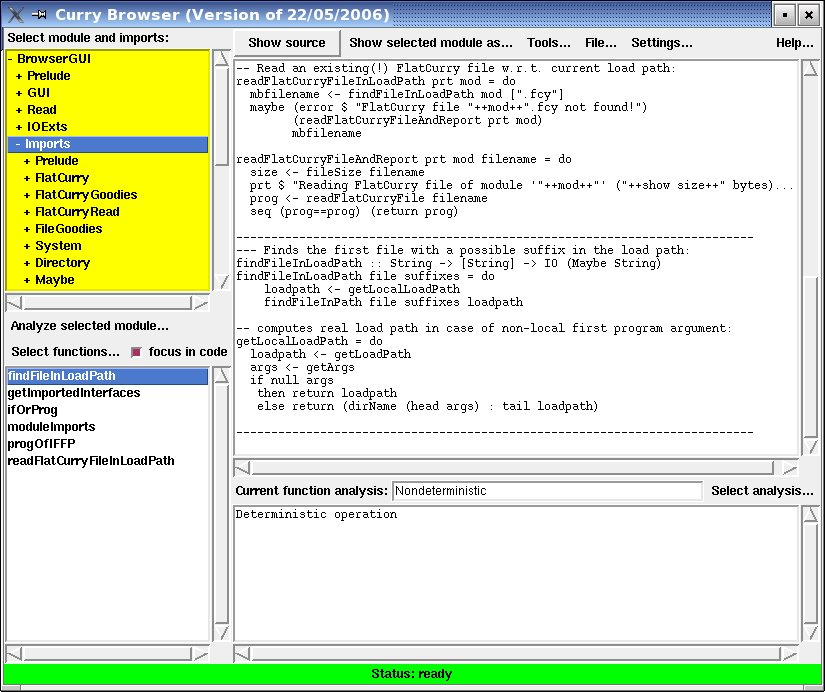
\includegraphics[scale=0.7]{currybrowser.jpg}
\end{center}
\caption{Snapshot of the main window of CurryBrowser\label{fig-currybrowser}}
\end{figure}
%
To get an impression of the use of \cb, Figure~\ref{fig-currybrowser}
shows a snapshot of its use on a particular application
(here: the implementation of \cb).
The upper list box in the left column shows the modules and their imports
in order to browse through the modules of an application.
Similarly to directory browsers, the list of imported modules of a module
can be opened or closed by clicking.
After selecting a module in the list of modules, its source code,
interface, or various other formats of the module can be shown
in the main (right) text area. For instance, one can show
pretty-printed versions of the intermediate flat programs (see below)
in order to see how local function definitions are translated by lambda lifting
\cite{Johnsson85}
or pattern matching is translated into case expressions \cite{Hanus97POPL,Wadler87}.
Since Curry is a language with parametric polymorphism and type inference,
programmers often omit the type signatures when defining functions.
Therefore, one can also view (and store) the selected module as source code where
missing type signatures are added.

Below the list box for selecting modules, there is a menu
(``Analyze selected module'') to analyze all functions
of the currently selected module at once. This is useful
to spot some functions of a module that could be problematic
in some application contexts, like functions that are impure (i.e., the result
depends on the evaluation time) or partially defined (i.e.,
not evaluable on all ground terms).
If such an analysis is selected,
the names of all functions are shown in the
lower list box of the left column (the ``function list'')
with prefixes indicating the properties of the individual functions.

The function list box can be also filled with functions
via the menu ``Select functions''. For instance, all functions
or only the exported functions defined in the currently selected
module can be shown there, or all functions from different modules
that are directly or indirectly called from
a currently selected function.
This list box is central to focus on a function in the
source code of some module or to analyze some function,
i.e., showing their properties. In order to focus on a function,
it is sufficient to check the ``focus on code'' button.
To analyze an individually selected function, one can
select an analysis from the list of available program analyses
(through the menu ``Select analysis'').
In this case, the analysis results are either shown
in the text box below the main text area
or visualized by separate tools, e.g., by a graph drawing tool for
visualizing call graphs.
Some analyses are local, i.e., they need only to consider the local definition
of this function (e.g., ``Calls directly,'' ``Overlapping rules,''
``Pattern completeness''),
where other analyses are global, i.e.,
they consider the definitions of all functions directly or indirectly called
by this function (e.g., ``Depends on,'' ``Solution complete,''
``Set-valued'').
%
Finally, there are a few additional tools integrated into \cb,
for instance, to visualize the import relation between all modules
as a dependency graph. These tools are available through the ``Tools'' menu.

More details about the use of \cb and all built-in analyses
are available through the ``Help'' menu of \cb.


\newpage

\section{CurryTest: A Tool for Testing Curry Programs}
\label{sec-currytest}

CurryTest\index{CurryTest}\index{testing programs}\index{program!testing}
is a simple tool in the PAKCS distribution to write
and run repeatable tests. CurryTest simplifies the task
of writing test cases for a module and executing them.
The tool is easy to use. Assume one has implemented a module \code{MyMod}
and wants to write some test cases to test its functionality,
making regression tests in future versions, etc.
For this purpose, there is a system library \code{Assertion}
(Section~\ref{Library:Assertion}) which
contains the necessary definitions for writing tests.
In particular, it exports an abstract polymorphic type \ccode{Assertion a}
together with the following operations:
\startprog
assertTrue      :: String -> Bool -> Assertion ()
assertEqual     :: String -> a -> a -> Assertion a
assertValues    :: String -> a -> [a] -> Assertion a
assertSolutions :: String -> (a->Success) -> [a] -> Assertion a
assertIO        :: String -> IO a -> a -> Assertion a
assertEqualIO   :: String -> IO a -> IO a -> Assertion a
\stopprog
The expression \ccode{assertTrue $s$ $b$}
is an assertion (named $s$) that the expression $b$ has the value \code{True}.
Similarly, the expression \ccode{assertEqual $s$ $e_1$ $e_2$}
asserts that the expressions $e_1$ and $e_2$
must be equal (i.e., \code{$e_1$==$e_2$} must hold),
the expression \ccode{assertValues $s$ $e$ $vs$} asserts
that $vs$ is the multiset of all values of $e$,
and the expression \ccode{assertSolutions $s$ $c$ $vs$} asserts
that the constraint abstraction $c$ has the multiset of solutions $vs$.
Furthermore, the expression \ccode{assertIO $s$ $a$ $v$}
asserts that the I/O action $a$ yields the value $v$ whenever it is
executed, and
the expression \ccode{assertEqualIO $s$ $a_1$ $a_2$}
asserts that the I/O actions $a_1$ and $a_2$ yields equal values.
The name $s$ provided as a first argument in each assertion
is used in the protocol produced by the test tool.

One can define a test program by importing the module
to be tested together with the module \code{Assertion} and defining
top-level functions of type \code{Assertion} in this module
(which must also be exported).
As an example, consider the following program
that can be used to test some list processing functions:
\startprog
\medskip
import List
import Assertion
\medskip
test1 = assertEqual     "++"     ([1,2]++[3,4]) [1,2,3,4]
\medskip
test2 = assertTrue      "all"    (all (<5) [1,2,3,4])
\medskip
test3 = assertSolutions "prefix" (\labs{}x -> let y free in  x\,++\,y =:= [1,2])
                                 [[],[1],[1,2]]
\medskip
\stopprog
For instance, \code{test1} asserts that the result of evaluating the
expression \code{([1,2]++[3,4])} is equal to \code{[1,2,3,4]}.

We can execute a test suite by the command\pindex{currytest}
\startprog
currytest testList
\stopprog
(\code{currytest} is a program stored in \code{$pakcshome$/bin}
where $pakcshome$ is the installation directory of PAKCS;
see Section~\ref{sec-general}).
In our example, \ccode{testList.curry} is the program containing the
definition of all assertions. This has the effect
that all exported top-level functions
of type \code{Assertion} are tested (i.e., the corresponding
assertions are checked) and the results
(\ccode{OK} or failure) are reported together with the name of each assertion.
%If failures occur, the complete test results are also
%written into a file named \ccode{testList.testlog}.''
For our example above, we obtain the following successful protocol:
\startprog
============================================================
Testing module "testList"...
OK: ++
OK: all
OK: prefix
All tests successfully passed.
============================================================
\stopprog
There is also a graphical interface that summarizes the results
more nicely.\footnote{Due to a bug in older versions of SICStus-Prolog,
it works only with SICStus-Prolog version 3.8.5 (or newer).}
In order to start this interface, one has to add the parameter
\ccode{--window} (or \ccode{-w}), e.g., executing a test suite by
\startprog
currytest --window testList
\stopprog
or
\startprog
currytest -w testList
\stopprog
A snapshot of the interface is shown in Figure~\ref{fig-currytest}.

\begin{figure}%[t]
\begin{center}
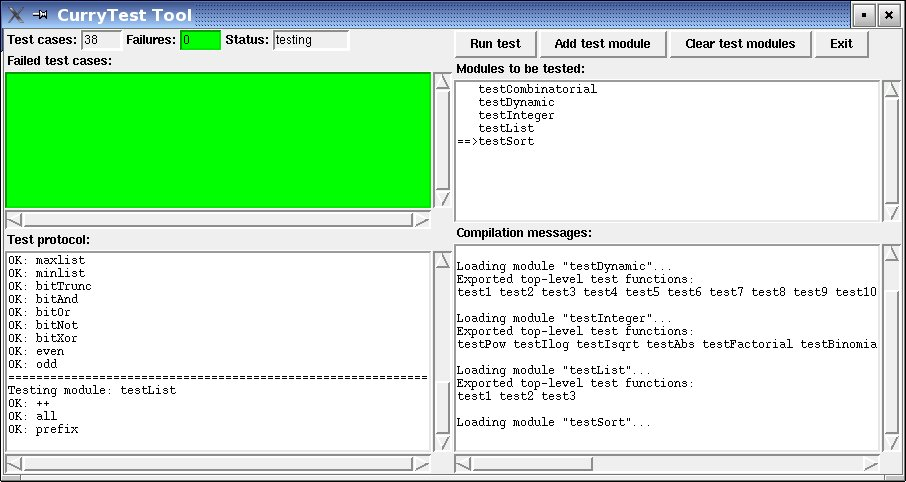
\includegraphics[scale=0.7]{currytest.jpg}
\end{center}
\caption{Snapshot of CurryTest's graphical interface\label{fig-currytest}}
\end{figure}


\newpage

\section{ERD2Curry: A Tool to Generate Programs from ER Specifications}
\label{sec-erd2curry}

ERD2Curry\index{ERD2Curry}\index{database programming}
is a tool to generate Curry code to access and manipulate data
persistently stored from
entity relationship diagrams.\index{entity relationship diagrams}
The idea of this tool is described in detail in
\cite{BrasselHanusMueller08PADL}.
Thus, we describe only the basic steps to use this tool
in the following.

If one creates an entity relationship diagram (ERD)
with the Umbrello UML Modeller, one has to store its
XML description in XMI format (as offered by Umbrello)
in a file, e.g., \ccode{myerd.xmi}.
This description can be compiled into a Curry program by the
command\pindex{erd2curry}
\startprog
erd2curry myerd.xmi
\stopprog
(\code{erd2curry} is a program stored in \code{$pakcshome$/bin}
where $pakcshome$ is the installation directory of PAKCS;
see Section~\ref{sec-general}).
If \code{MyData} is the name of the ERD, the Curry program file
\ccode{MyData.curry} is generated containing all the necessary
database access code as described in \cite{BrasselHanusMueller08PADL}.

If one does not want to use the Umbrello UML Modeller,
one can also create a textual description of the ERD
as a Curry term of type \code{ERD}
(w.r.t.\ the type definition given in module
\code{$pakcshome$/tools/erd2curry/ERD.curry})
and store it in some file, e.g., \ccode{myerd.term}.
This description can be compiled into a Curry program by the
command\pindex{erd2curry}
\startprog
erd2curry -t myerd.term
\stopprog
%
There is also the possibility to visualize an ERD term
as a graph with the graph visualization program \code{dotty}
(for this purpose, it might be necessary to adapt the definition
of the operation \code{dotCmd} in
\code{$pakcshome$/tools/erd2curry/ERD2Graph.curry}
according to your local environment).
This can be done by the command
\startprog
erd2curry -v myerd.term
\stopprog

\paragraph{Inclusion in the Curry application:}
To compile the generated database code, either
include the directory \code{$pakcshome$/tools/erd2curry}
into your Curry load path
(e.g., by setting  the environment variable
\ccode{CURRYPATH}\pindex{CURRYPATH}, see also Section~\ref{sec-modules})
or copy the file
\code{$pakcshome$/tools/erd2curry/ERDGeneric.curry}
into the directory of the generated database code.


\newpage

\section{UI: Declarative Programming of User Interfaces}
\label{sec-ui}

The PAKCS distribution contains a collection of libraries
to implement graphical user interfaces\index{user interface}
as well as web-based user interfaces
from declarative descriptions.
Exploiting these libraries, it is possible
to define the structure and functionality of a user interface
independent from the concrete technology.
Thus, a graphical user interface or a web-based user interface
can be generated from the same description by simply changing
the imported libraries.
This programming technique is described in detail in
\cite{HanusKluss09PADL}.

The libraries implementing these user interfaces are contained
in the directory
\startprog
$pakcshome$/tools/ui
\stopprog
Thus, in order to compile programs containing such user interface
specifications, one has to
include the directory \code{$pakcshome$/tools/ui}
into the Curry load path
(e.g., by setting  the environment variable
\ccode{CURRYPATH}\pindex{CURRYPATH}, see also Section~\ref{sec-modules}).
The directory
\startprog
$pakcshome$/tools/ui/examples
\stopprog
contains a few examples for such user interface specifications.


\newpage

\section{Preprocessing FlatCurry Files}
\label{sec-pakcspp}

The current parser allows to apply transformations on the intermediate
FlatCurry files after they are generated from the
corresponding Curry source file.
Currently, only the FlatCurry file corresponding to the main module
can be transformed.

A transformation can be specified as follows:
\begin{enumerate}
\item {\bf Options to \code{pakcs/bin/parsecurry}:}
\begin{description}
\item[\fbox{\code{--fpopt}}]\pindex{-fpopt}
Apply functional pattern optimization
(see \code{pakcs/tools/optimize/NonStrictOpt.curry} for details).

\item[\fbox{\code{--compact}}]\pindex{--compact}
Apply code compactification after parsing, i.e., transform the main
module and all its imported into one module and delete all
non-accessible functions.

\item[\fbox{\code{--compactexport}}]
Similar to \code{--compact} but delete all functions that are not accessible
from the exported functions of the main module.

\item[\fbox{\code{--compactmain:f}}]
Similar to \code{--compact} but delete all functions that are not accessible
from the function \ccode{f} of the main module.

\item[\fbox{\code{--fcypp cmd}}]\pindex{--fcypp}
Apply command \code{cmd} to the main module after parsing. This is useful to
integrate your own transformation into the compilation process.
Note that the command \ccode{cmd prog} should perform a transformation
on the FlatCurry file \code{prog.fcy}, i.e., it replaces the FlatCurry
file by a new one.
\end{description}

\item {\bf Setting the environment variable \code{FCYPP}:}\pindex{FCYPP}\\
For instance, setting \code{FCYPP} by
\startprog
export FCYPP="--fpopt"
\stopprog
will apply the functional pattern optimization if programs are compiled
and loaded in the PAKCS programming environment.


\item {\bf Putting options into the source code:}\pindex{PAKCS_OPTION_FCYPP}\\
If the source code contains a line with a comment of the form (the comment
must start at the beginning of the line)
\startprog
\{-\# PAKCS_OPTION_FCYPP <options> \#-\}
\stopprog
then the transformations specified by \code{<options>} are applied after
translating the source code into FlatCurry code. For instance,
the functional pattern optimization can be set by the comment
\startprog
\{-\# PAKCS_OPTION_FCYPP --fpopt \#-\}
\stopprog
in the source code. Note that this comment must be in a single line 
of the source program. If there are multiple lines containing such comments,
only the first one will be considered.
\end{enumerate}
\paragraph{Multiple options:}
Note that an arbitrary number of transformations can be specified
by the methods described above.
If several specifications for preprocessing FlatCurry files are used,
they are executed in the following order:
\begin{enumerate}
\item all transformations specified by the environemnt variable
\code{FCYPP} (from left to right)
\item all transformations specified as command line options of parsecurry
   (from left to right)
\item all transformations specified by a comment line in the source code
   (from left to right)
\end{enumerate}


\newpage

\section{Technical Problems}

Due to the fact that Curry is intended to implement
distributed systems (see Appendix~\ref{sec-ports}),
it might be possible that some technical problems
arise due to the use of sockets for implementing these
features. Therefore, this section gives some information
about the technical requirements of PAKCS and how to solve
problems due to these requirements.

There is one fixed port that is used by the implementation of PAKCS:
\begin{description}
\item[Port 8766:] This port is used by the
{\bf Curry Port Name Server} (CPNS) to implement symbolic names for
ports in Curry (see Appendix~\ref{sec-ports}).
If some other process uses this port on the machine,
the distribution facilities defined in the module \code{Ports}
(see Appendix~\ref{sec-ports}) cannot be used.
\end{description}
If these features do not work, you can try to find out
whether this port is in use by the shell command
\ccode{netstat -a | fgrep 8766} (or similar).

The CPNS is implemented as a demon listening on its port 8766
in order to serve requests about registering a new symbolic
name for a Curry port or asking the physical port number
of a Curry port. The demon will be automatically started for
the first time on a machine when a user compiles a program
using Curry ports. It can also be manually started and terminated by the
scripts \code{$pakcshome$/cpns/start} and
\code{$pakcshome$/cpns/stop}.
If the demon is already running, the command \code{$pakcshome$/cpns/start}
does nothing (so it can be always executed
before invoking a Curry program using ports).

If you detect any further technical problem,
please write to
\begin{center}
\code{mh@informatik.uni-kiel.de}
\end{center}

\newpage

\addcontentsline{toc}{section}{Bibliography}
\bibliography{manual}
\bibliographystyle{plain}

\newpage
\appendix

\section{Libraries of the PAKCS Distribution}
\label{sec:libraries}

{\setlength{\parindent}{0.0cm}

The PAKCS compiler system provides an extensive collection
of libraries for application programming.
The libraries for arithmetic constraints over real numbers,
finite domain constraints,
ports for concurrent and distributed programming, and
meta-programming by representing Curry programs in Curry
are described in the following subsection in more detail.
The complete set of libraries with all exported types and functions
are described in the further subsections.
For a more detailed online documentation of all libraries of PAKCS,
see \url{http://www.informatik.uni-kiel.de/~pakcs/lib/index.html}.

\subsection{Constraints, Ports, Meta-Programming}

\subsubsection{Arithmetic Constraints}

The primitive entities for the use of arithmetic constraints
are defined in the system module \code{CLPR}
(cf.\ Section~\ref{sec-modules}), i.e., in order to use them,
the program must contain the import declaration
\startprog
import CLPR
\stopprog
Floating point arithmetic is supported in PAKCS
via arithmetic constraints, i.e., the equational constraint
\ccode{2.3 +.~x =:= 5.5} is solved by binding \code{x} to \code{3.2}
(rather than suspending the evaluation of the addition,
as in corresponding constraints on integers like
\ccode{3+x=:=5}). All operations related to
floating point numbers are suffixed by \ccode{.}.
The following functions and constraints on floating point
numbers are supported in PAKCS:
\begin{description}
\item[\code{(+.)   :: Float -> Float -> Float}]~\\
Addition on floating point numbers.
\item[\code{(-.)   :: Float -> Float -> Float}]~\\
Subtraction on floating point numbers.
\item[\code{(*.)   :: Float -> Float -> Float}]~\\
Multiplication on floating point numbers.
\item[\code{(/.)   :: Float -> Float -> Float}]~\\
Division on floating point numbers.
\item[\code{(<.)   :: Float -> Float -> Success}]~\\
Comparing two floating point numbers with the ``less than'' relation.
\item[\code{(>.)   :: Float -> Float -> Success}]~\\
Comparing two floating point numbers with the ``greater than'' relation.
\item[\code{(<=.)  :: Float -> Float -> Success}]~\\
Comparing two floating point numbers with the ``less than or equal'' relation.
\item[\code{(>=.)  :: Float -> Float -> Success}]~\\
Comparing two floating point numbers with the ``greater than or equal''
relation.
\item[\code{i2f    :: Int -> Float}]~\\
Converting an integer number into a floating point number.
\end{description}
As an example, consider a constraint \code{mortgage}
which relates the principal \code{p},
the lifetime of the mortgage in months \code{t},
the monthly interest rate \code{ir},
the monthly repayment \code{r},
and the outstanding balance at the end of the lifetime \code{b}.
The financial calculations
can be defined by the following two rules in Curry (the second rule
describes the repeated accumulation of the interest):
\startprog
~
import CLPR
~
mortgage p t ir r b | t >. 0.0 \& t <=. 1.0  --lifetime not more than 1 month?
                    =  b =:= p *. (1.0 +. t *. ir) -. t*.r \vspace{1ex}
mortgage p t ir r b | t >. 1.0               --lifetime more than 1 month?
                    =  mortgage (p *. (1.0+.ir)-.r) (t-.1.0) ir r b
~
\stopprog
Then we can calculate the monthly payment for paying back
a loan of \$100,000 in 15 years with a monthly interest rate of 1\%
by solving the goal
\startprog
mortgage 100000.0 180.0 0.01 r 0.0
\stopprog
which yields the solution \code{r=1200.17}.

Note that only linear arithmetic equalities or inequalities
are solved by the constraint solver. Non-linear constraints
like \ccode{x *.~x =:= 4.0} are suspended until they become
linear.


\subsubsection{Finite Domain Constraints}

Finite domain constraints are constraints where all variables
can only take a finite number of possible values.
For simplicity, the domain of finite domain variables are
identified with a subset of the integers, i.e., the type
of a finite domain variable is \code{Int}. The arithmetic
operations related to finite domain variables are suffixed by \ccode{\#}.
The following functions and constraints for finite domain constraint solving
are currently supported in PAKCS:\footnote{Note that
this library is based on the corresponding library of SICStus-Prolog
but does not implement the complete functionality of the SICStus-Prolog library.
However, using the PAKCS interface for external functions (see
Appendix~\ref{sec-external-functions}), it is relatively
easy to provide the complete functionality.}

\begin{description}
\item[\code{domain :: [Int] -> Int -> Int -> Success}]~\\
The constraint \ccode{domain [$x_1,\ldots,x_n$] $l$ $u$}
is satisfied if the domain of all variables $x_i$ is the interval $[l,u]$.
\item[\code{(+\#)   :: Int -> Int -> Int}]~\\
Addition on finite domain values.
\item[\code{(-\#)   :: Int -> Int -> Int}]~\\
Subtraction on finite domain values.
\item[\code{(*\#)   :: Int -> Int -> Int}]~\\
Multiplication on finite domain values.
\item[\code{(=\#)   :: Int -> Int -> Success}]~\\
Equality of finite domain values.
\item[\code{(/=\#)  :: Int -> Int -> Success}]~\\
Disequality of finite domain values.
\item[\code{(<\#)   :: Int -> Int -> Success}]~\\
``less than'' relation on finite domain values.
\item[\code{(<=\#)  :: Int -> Int -> Success}]~\\
``less than or equal'' relation on finite domain values.
\item[\code{(>\#)   :: Int -> Int -> Success}]~\\
``greater than'' relation on finite domain values.
\item[\code{(>=\#)  :: Int -> Int -> Success}]~\\
``greater than or equal'' relation on finite domain values.
\item[\code{sum :: [Int] -> (Int -> Int -> Success) -> Int -> Success}]~\\
The constraint \ccode{sum [$x_1,\ldots,x_n$] $op$ $x$}
is satisfied if all $x_1+\cdots + x_n \mathrel{op} x$ is satisfied,
where $op$ is one of the above finite domain constraint relations
(e.g., \ccode{=\#}).
\item[\code{scalar_product :: [Int] -> [Int] -> (Int -> Int -> Success) -> Int -> Success}]~\\
The constraint \ccode{scalar_product [$c_1,\ldots,c_n$] [$x_1,\ldots,x_n$] $op$ $x$}
is satisfied if all $c_1 x_1+\cdots + c_n x_n \mathrel{op} x$ is satisfied,
where $op$ is one of the above finite domain constraint relations.
\item[\code{count :: Int -> [Int] -> (Int -> Int -> Success) -> Int -> Success}]~\\
The constraint \ccode{count $k$ [$x_1,\ldots,x_n$] $op$ $x$}
is satisfied if all $k \mathrel{op} x$ is satisfied,
where $n$ is the number of the $x_i$ that are equal to $k$ and
$op$ is one of the above finite domain constraint relations.
\item[\code{all_different :: [Int] -> Success}]~\\
The constraint \ccode{all_different [$x_1,\ldots,x_n$]}
is satisfied if all $x_i$ have pairwise different values.
\item[\code{labeling :: [LabelingOption] -> [Int] -> Success}]~\\
The constraint \ccode{labeling $os$ [$x_1,\ldots,x_n$]}
non-deterministically instantiates all $x_i$ to the values
of their domain according to the options $os$ (see the module documentation
for further details about these options).
\end{description}
These entities are defined in the system module \code{CLPFD}
(cf.\ Section~\ref{sec-modules}), i.e., in order to use it,
the program must contain the import declaration
\startprog
import CLPFD
\stopprog
As an example, consider the classical \ccode{send+more=money} problem
where each letter must be replaced by a different digit such that this
equation is valid and there are no leading zeros.
The usual way to solve finite domain constraint problems
is to specify the domain of the involved variables followed
by a specification of the constraints and the labeling
of the constraint variables in order to start the search for solutions.
Thus, the \ccode{send+more=money} problem can be solved as follows:
\startprog
~
import CLPFD
~
smm l =
        l =:= [s,e,n,d,m,o,r,y] \&
        domain l 0 9 \&
        s >\# 0 \&
        m >\# 0 \&
        all_different l  \&
                         1000 *\# s +\# 100 *\# e +\# 10 *\# n +\# d
        +\#               1000 *\# m +\# 100 *\# o +\# 10 *\# r +\# e
        =\# 10000 *\# m +\# 1000 *\# o +\# 100 *\# n +\# 10 *\# e +\# y \&
        labeling [FirstFail] l
        where s,e,n,d,m,o,r,y free
~
\stopprog
Then we can solve this problem by evaluating the goal
\ccode{smm [s,e,n,d,m,o,r,y]} which yields the unique solution
\code{\{s=9,e=5,n=6,d=7,m=1,o=0,r=8,y=2\}}.


\subsubsection{Ports: Distributed Programming in Curry}
\label{sec-ports}

To support the development of concurrent and distributed applications,
PAKCS supports internal and external ports\index{ports} as
described in \cite{Hanus99PPDP}.
Since \cite{Hanus99PPDP} contains a detailed description of this
concept together with various programming examples, we only summarize here
the functions and constraints supported for ports in PAKCS.

The basic datatypes, functions, and constraints for ports
are defined in the system module \code{Ports}
(cf.\ Section~\ref{sec-modules}), i.e., in order to use ports,
the program must contain the import declaration
\startprog
import Ports
\stopprog
This declaration includes the following entities in the program:
\begin{description}
\item[\code{Port a}\pindex{Port}]~\\
This is the datatype of a port to which one can send messages of type \code{a}.

\item[\code{openPort :: Port a -> [a] -> Success}]~\\
The constraint \ccode{openPort p s}\pindex{openPort}
establishes a new \emph{internal port}
\code{p} with an associated message stream \code{s}. \code{p} and \code{s} must be
unbound variables,
otherwise the constraint fails (and causes a runtime error).

\item[\code{send :: a -> Port a -> Success}]~\\
The constraint \ccode{send m p}\pindex{send}
is satisfied if \code{p} is constrained
to contain the message \code{m}, i.e., \code{m} will be sent to the port
\code{p} so that it appears in the corresponding stream.

\item[\code{doSend :: a -> Port a -> IO ()}]~\\
The I/O action \ccode{doSend m p}\pindex{doSend} solves the constraint
\ccode{send m p} and returns nothing.

\item[\code{openNamedPort :: String -> IO [a]}]~\\
The I/O action \ccode{openNamedPort n}\pindex{openNamedPort}
opens a new \emph{external port} with
symbolic name \code{n} and returns the associated stream of messages.

\item[\code{connectPort :: String -> IO (Port a)}]~\\
The I/O action \ccode{connectPort n}\pindex{connectPort}
returns a port with symbolic name
\code{n} (i.e., \code{n} must have the form ``\emph{portname@machine})
to which one can send messages by the \code{send} constraint.
Currently, no dynamic type checking is done for external ports,
i.e., sending messages of the wrong type to a port might lead to
a failure of the receiver.
\end{description}

\paragraph{Restrictions:}
Every expression, possibly containing logical variables, can be sent to
a port. However, as discussed in \cite{Hanus99PPDP},
port communication is strict, i.e., the expression is
evaluated to normal form before sending it by the
constraint \code{send}. Furthermore, if messages containing
logical variables are sent to \emph{external ports},
the behavior is as follows:
\begin{enumerate}
\item The sender waits until all logical variables in the message
have been bound by the receiver.
\item The binding of a logical variable received by a process
is sent back to the sender of this logical variable only if
it is bound to a \emph{ground} term, i.e., as long as the binding contains
logical variables, the sender is not informed about the binding
and, therefore, the sender waits.
\end{enumerate}

\paragraph{External ports on local machines:}
The implementation of external ports assumes that the
host machine running the application is connected to the Internet
(i.e., it uses the standard IP address of the host machine
for message sending). If this is not the case and the application
should be tested by using external ports only on the local host
without a connection to the Internet,
the environment variable \ccode{PAKCS_LOCALHOST}\pindex{PAKCS_LOCALHOST}
must be set to \ccode{yes}
\emph{before PAKCS system is started}.
In this case, the IP address \code{127.0.0.1} and the hostname
\ccode{localhost} are used for identifying the local machine.

\paragraph{Selection of Unix sockets for external ports:}
The implementation of ports uses sockets to communicate
messages sent to external ports.
Thus, if a Curry program uses the
I/O action \code{openNamedPort}\pindex{openNamedPort}
to establish an externally visible server,
PAKCS selects a Unix socket for the port communication.
Usually, a free socket is selected by the operating system.
If the socket number should be fixed in an application (e.g.,
because of the use of firewalls\index{firewall} that allow only
communication over particular sockets), then one
can set the environment variable \ccode{PAKCS_SOCKET}\pindex{PAKCS_SOCKET}
to a distinguished socket number before the PAKCS system is started.
This has the effect that PAKCS uses only this socket
number for communication (even for several external ports
used in the same application program).

\paragraph{Debugging:}
To debug distributed systems,
it is sometimes helpful to see all messages sent to external ports.
This is supported by the environment variable
\ccode{PAKCS_TRACEPORTS}.\pindex{PAKCS_TRACEPORTS}
If this variable is set to \ccode{yes}
\emph{before the PAKCS system is started}, then all
connections to external ports and all
messages sent and received on external ports are
printed on the standard error stream.


\subsubsection{AbstractCurry and FlatCurry: Meta-Programming in Curry}
\label{sec-flatcurry}

\index{AbstractCurry}
\index{FlatCurry}
To support meta-programming, i.e., the manipulation of Curry programs
in Curry, there are system modules \code{FlatCurry} and \code{AbstractCurry}
(stored in the directory \ccode{$pakcshome$/lib/meta})
which define datatypes for the representation
of Curry programs.
\code{AbstractCurry} is a more direct representation of a Curry program,
whereas \code{FlatCurry} is a simplified representation
where local function definitions are replaced by global definitions
(i.e., lambda lifting has been performed) and pattern matching
is translated into explicit case/or expressions.
Thus, \code{FlatCurry} can be used for more back-end oriented
program manipulations (or, for writing new back ends for Curry),
whereas \code{AbstractCurry} is intended for manipulations of
programs that are more oriented towards the source program.

Both modules contain predefined I/O actions to read programs
in the \code{AbstractCurry} (\code{readCurry}\pindex{readCurry})
or \code{FlatCurry}
(\code{readFlatCurry}\pindex{readFlatCurry}) format.
These actions parse the corresponding source program and return
a data term representing this program (according to the definitions
in the modules \code{AbstractCurry} and \code{FlatCurry}).

Since all datatypes are explained in detail in these modules,
we refer to the online documentation\footnote{%
\url{http://www.informatik.uni-kiel.de/~pakcs/lib/CDOC/FlatCurry.html} and
\url{http://www.informatik.uni-kiel.de/~pakcs/lib/CDOC/AbstractCurry.html}}
of these modules.

As an example, consider a program file \ccode{test.curry}
containing the following two lines:
\startprog
rev []     = []
rev (x:xs) = (rev xs) ++ [x]
\stopprog
Then the I/O action \code{(FlatCurry.readFlatCurry "test")} returns the
following term:
\startprog
 (Prog "test"
  ["Prelude"]
  []
  [Func ("test","rev") 1 Public
        (FuncType (TCons ("Prelude","[]") [(TVar 0)])
                  (TCons ("Prelude","[]") [(TVar 0)]))
        (Rule [0]
           (Case Flex (Var 0)
              [Branch (Pattern ("Prelude","[]") [])
                  (Comb ConsCall ("Prelude","[]") []),
               Branch (Pattern ("Prelude",":") [1,2])
                  (Comb FuncCall ("Prelude","++")
                        [Comb FuncCall ("test","rev") [Var 2],
                         Comb ConsCall ("Prelude",":")
                              [Var 1,Comb ConsCall ("Prelude","[]") []]
                        ])
              ]))]
  []
 )
\stopprog


%%%%%%%%%%%%%%%%%%%%%%%%%%%%%%%%%%%%%%%%%%%%%%%%%%%%%%%%%%%%%%%%%%%%%%%%%
% Definitions in order to LaTeX documents generated by "currydoc --tex"
%%%%%%%%%%%%%%%%%%%%%%%%%%%%%%%%%%%%%%%%%%%%%%%%%%%%%%%%%%%%%%%%%%%%%%%%%

\newcommand{\currymodule}[1]{\subsubsection{Library #1}\label{Library:#1}}
\newcommand{\currytypesstart}{\subsubsection*{Exported types:}}
\newcommand{\currytypesstop}{}
\newcommand{\currytypesynstart}[2]{{\tt type #2}\pindex{#1} \begin{quote}}
\newcommand{\currytypesynstop}{\end{quote}}
\newcommand{\currydatastart}[1]{{\tt data #1}\pindex{#1} \begin{quote}}
\newcommand{\currydatacons}{\end{quote}%
\begin{itemize}\item[] \hspace{-4ex}\emph{Exported constructors:}}
\newcommand{\currydatastop}{\end{itemize}}
\newcommand{\curryconsstart}[2]{\item {\tt #1~::~#2}\par}
\newcommand{\curryfuncstart}{\subsubsection*{Exported functions:}}
\newcommand{\curryfuncstop}{}
\newcommand{\curryfunctionstart}[2]{#2\pindex{#1}\begin{quote}}
\newcommand{\curryfunctionstop}{\end{quote}}
\newcommand{\curryfuncsig}[2]{{\tt #1~::~#2}}


\subsection{General Libraries}

\input{lib/AllSolutions}
\input{lib/Assertion}
\input{lib/Char}
\input{lib/CLPFD}
\input{lib/CLPR}
\input{lib/CLPB}
\input{lib/Combinatorial}
\input{lib/Constraint}
\input{lib/CSV}
\input{lib/Database}
\input{lib/DaVinci}
\input{lib/Directory}
\input{lib/Dynamic}
\input{lib/FileGoodies}
\input{lib/Float}
\input{lib/Global}
\input{lib/GlobalVariable}
\input{lib/GUI}
\input{lib/Integer}
\input{lib/IO}
\input{lib/IOExts}
\input{lib/JavaScript}
\input{lib/KeyDatabase}
\input{lib/KeyDatabaseSQLite}
\input{lib/KeyDB}
\input{lib/List}
\input{lib/Maybe}
\input{lib/NamedSocket}
\input{lib/Parser}
\input{lib/Ports}
\input{lib/Pretty}
\input{lib/Profile}
\input{lib/PropertyFile}
\input{lib/Read}
\input{lib/ReadNumeric}
\input{lib/ReadShowTerm}
\input{lib/SetFunctions}
\input{lib/Socket}
\input{lib/System}
\input{lib/Time}
%\input{lib/Tk}
\input{lib/Unsafe}


\subsection{Data Structures and Algorithms}

\input{lib/Array}
\input{lib/Dequeue}
\input{lib/FiniteMap}
\input{lib/GraphInductive}
\input{lib/Random}
\input{lib/RedBlackTree}
\input{lib/SetRBT}
\input{lib/Sort}
\input{lib/TableRBT}
\input{lib/Traversal}

\subsection{Libraries for Web Applications}

\input{lib/CategorizedHtmlList}
\input{lib/HTML}
\input{lib/HtmlParser}
\input{lib/Mail}
\input{lib/Markdown}
\input{lib/WUI}
\input{lib/URL}
\input{lib/XML}
\input{lib/XmlConv}

\subsection{Libraries for Meta-Programming}

\input{lib/AbstractCurry}
\input{lib/AbstractCurryPrinter}
\input{lib/CompactFlatCurry}
\input{lib/CurryStringClassifier}
\input{lib/FlatCurry}
\input{lib/FlatCurryGoodies}
\input{lib/FlatCurryRead}
\input{lib/FlatCurryShow}
\input{lib/FlatCurryTools}
\input{lib/FlatCurryXML}
\input{lib/FlexRigid}
\input{lib/PrettyAbstract}

} % end setlength parindent

\newpage

\input{markdown_syntax}

\newpage

\begin{figure}%[t]
\begin{center}
 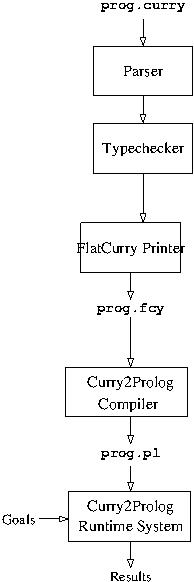
\includegraphics[scale=0.85]{pakcs_overview.jpg}
\end{center}\vspace{-5ex}
\caption{Overview of PAKCS\label{fig-pakcs}}
\end{figure}

\section{Overview of the PAKCS Distribution}

A schematic overview of the various components contained in
the distribution of PAKCS and the
translation process of programs inside PAKCS is shown in
Figure~\ref{fig-pakcs} on page~\pageref{fig-pakcs}.
In this figure, boxes denote different components of PAKCS
and names in boldface denote files containing
various intermediate representations during the translation
process (see Section~\ref{sec-auxfiles} below).
The PAKCS distribution contains a front end for reading (parsing and
type checking) Curry programs that can be also used by
other Curry implementations.
The back end (formerly known as ``Curry2Prolog''\index{Curry2Prolog})
compiles Curry programs into Prolog programs.
It also support constraint solvers for
arithmetic constraints over real numbers and finite domain constraints,
and further libraries for GUI programming, meta-programming etc.
Currently, it does not implement encapsulated search in full generality
(only a strict version of \code{findall} is supported),
and concurrent threads are not executed in a fair manner.


\newpage

\section{Auxiliary Files}
\label{sec-auxfiles}

During the translation and execution of a Curry program with PAKCS,
various intermediate representations of the source program are created
and stored in different files which are shortly explained in this section.
If you use the PAKCS, it is not necessary to know about
these auxiliary files because they are automatically generated
and updated. You should only remember the command for deleting
all auxiliary files (\ccode{cleancurry}, see Section~\ref{sec-general})
to clean up your directories.

The various components of PAKCS create
the following auxiliary files.
\begin{description}
\item[\code{prog.fcy}:] This file contains the Curry program
in the so-called ``FlatCurry'' representation where all functions are global
(i.e., lambda lifting has been performed) and pattern matching
is translated into explicit case/or expressions
(compare Appendix~\ref{sec-flatcurry}).
This representation might be useful for other back ends and
compilers for Curry and is the basis doing meta-programming in Curry.
This file is implicitly
generated when a program is read by PAKCS.
It can be also explicitly generated by the command\pindex{parsecurry}
\startprog
parsecurry --flat prog
\stopprog
The FlatCurry representation of a Curry program is usually
generated by the front-end after parsing, type checking and eliminating
local declarations.
If $dir$ is the directory where the Curry program is stored,
the corresponding FlatCurry program is stored in the directory
\ccode{$dir$/.curry}.

\item[\code{prog.fint}:] This file contains the interface
of the program in the so-called ``FlatCurry'' representation,
i.e., it is similar to \code{prog.fcy} but contains only exported
entities and the bodies of all functions omitted (i.e., ``external'').
This representation is useful for providing a fast access
to module interfaces.
This file is implicitly generated by the command\pindex{parsecurry}
\startprog
parsecurry --flat prog
\stopprog
and stored in the same directory as \code{prog.fcy}.

\item[\code{prog.pl}:] This file contains a Prolog program
as the result of translating the Curry program with PAKCS.
If $dir$ is the directory where the Curry program is stored,
the corresponding Prolog program is stored in the directory
\ccode{$dir$/.curry/.pakcs}.

\item[\code{prog.po}:] This file contains the Prolog program
\code{prog.pl} in an intermediate format for faster loading.
This file is stored in the same directory as \code{prog.pl}.

\item[\code{prog.state}:] This file contains the saved state
after compiling and saving a program with PAKCS
(see Section~\ref{sec-use-curry2prolog}).

\end{description}


\newpage


\section{Changing the Prelude or System Modules}

The standard prelude, which is automatically imported into each Curry program,
and all system modules containing datatypes and functions
useful for application programming
(cf.\ Appendix~\ref{sec:libraries})
are stored in the system module directory \ccode{$pakcshome$/lib}
(and its subdirectories).
If you change any of these modules,
you have to recompile the complete system by
executing \code{make} in the directory $pakcshome$.



\newpage

\section{External Functions}
\label{sec-external-functions}

\index{function!external}\index{external function}
Currently, PAKCS has no general interface to external functions.
Therefore, if a new external function should be added
to the system, this function must be declared as \code{external}
in the Curry source code
and then an implementation for this external function
must be inserted in the corresponding back end.
An external function is defined as follows in the Curry source code:
\begin{enumerate}
\item
Add a type declaration for the external function somewhere
in the body of the appropriate file (usually, the prelude
or some system module).
\item
For external functions it is not allowed to define any
rule since their semantics is determined by an external implementation.
Instead of the defining rules, you have to write
\startprog
f external
\stopprog
somewhere in the file containing the type declaration for 
the external function \code{f}.
\end{enumerate}
For instance, the addition on integers can be declared as
an external function as follows:
\startprog
(+) :: Int -> Int -> Int
(+) external
\stopprog
The further modifications to be done for an inclusion of
an external function has to be done in the back end.
A new external function is added to the back end of PAKCS
by informing the compiler about the existence of an external function
and adding an implementation of this function in the run-time
system. Therefore, the following items must be added
in the PAKCS compiler system:
\begin{enumerate}
\item
If the Curry module \code{Mod} contains external functions,
there must be a file named \code{Mod.prim_c2p} containing the
specification of these external functions. The contents of this file
is in XML format and has the following general structure:\footnote{%
\url{http://www.informatik.uni-kiel.de/~pakcs/primitives.dtd} contains a DTD
describing the exact structure of these files.}
\startprog
<primitives>
  \emph{specification of external function $f_1$}
  \ldots
  \emph{specification of external function $f_n$}
</primitives>
\stopprog
The specification of an external function $f$
with arity $n$ has the form
\startprog
<primitive name="$f$" arity="$n$">
  <library>lib</library>
  <entry>pred</entry>
</primitive>
\stopprog
where \code{lib} is the Prolog library (stored in the directory of the
Curry module or in the global directory
\code{$pakcshome$/curry2prolog/lib_src}) containing the code implementing this
function and \code{pred} is a predicate name in this library
implementing this function. Note that the function $f$ must be
declared in module \code{Mod}: either as an external function
or defined in Curry by equations. In the latter case,
the Curry definition is not translated but calls to this function
are redirected to the Prolog code specified above.

Furthermore, the list of specifications can also contain entries of the form
\startprog
<ignore name="$f$" arity="$n$" />
\stopprog
for functions $f$ with arity $n$ that are declared in module \code{Mod}
but should be ignored for code generation, e.g., since they are
never called w.r.t.\ to the current implementation of external functions.
For instance, this is useful when functions that can
be defined in Curry should be (usually more efficiently) are implemented
as external functions.

Note that the arguments are passed in their current (possibly unevaluated) form.
Thus, if the external function requires the arguments to be evaluated
in a particular form, this must be done before calling the external function.
For instance, the external function for adding two integers
requires that both arguments must be evaluated to non-variable head normal form
(which is identical to the ground constructor normal form). Therefore,
the function \ccode{+} is specified in the prelude by
\startprog
(+)   :: Int -> Int -> Int
x + y = (prim_Int_plus \$\# y) \$\# x
\medskip
prim_Int_plus :: Int -> Int -> Int
prim_Int_plus external
\stopprog
where \code{prim_Int_plus} is the actual external function implementing
the addition on integers. Consequently, the specification file
\code{Prelude.prim_c2p} has an entry of the form
\startprog
<primitive name="prim_Int_plus" arity="2">
  <library>prim_standard</library>
  <entry>prim_Int_plus</entry>
</primitive>
\stopprog
where the Prolog library \code{prim_standard.pl} contains the Prolog code
implementing this function.

\item
For most external functions, a \emph{standard interface} is
generated by the compiler so that an $n$-ary function can be
implemented by an $(n+1)$-ary predicate where the last argument must
be instantiated to the result of evaluating the function.  The
standard interface can be used if all arguments are ensured to be
fully evaluated (e.g., see definition of \code{(+)} above) and no
suspension control is necessary, i.e., it is ensured that the
external function call does not suspend for all arguments.
Otherwise, the raw interface (see below) must be used.  For
instance, the Prolog code implementing \code{prim_Int_plus}
contained in the Prolog library \code{prim_standard.pl} is as
follows (note that the arguments of \code{(+)} are passed in reverse
order to \code{prim_Int_plus} in order to ensure a left-to-right
evaluation of the original arguments by the calls to \code{(\$\#)}):
\startprog
prim_Int_plus(Y,X,R) :- R is X+Y.
\stopprog

\item
The \emph{standard interface for I/O actions}, i.e., external functions
with result type \code{IO~a}, assumes that the I/O action
is implemented as a predicate (with a possible side effect)
that instantiates the last argument to the returned value of type \ccode{a}.
For instance, the primitive predicate \code{prim_getChar}
implementing prelude I/O action \code{getChar}
can be implemented by the Prolog code
\startprog
prim_getChar(C) :- get_code(N), char_int(C,N).
\stopprog
where \code{char_int} is a predicate relating the internal
Curry representation of a character with its ASCII value.

\item
If some arguments passed to the external functions are not fully evaluated
or the external function might suspend, the implementation must follow
the structure of the PAKCS run-time system by using
the \emph{raw interface}. In this case, the name of the external entry
must be suffixed by \ccode{[raw]} in the \code{prim_c2p} file.
For instance, if we want to use the raw interface for the external function
\code{prim_Int_plus},
the specification file \code{Prelude.prim_c2p} must have an entry of the form
\startprog
<primitive name="prim_Int_plus" arity="2">
  <library>prim_standard</library>
  <entry>prim_Int_plus[raw]</entry>
</primitive>
\stopprog
In the raw interface, the actual implementation of an $n$-ary external function consists
of the definition of an $(n+3)$-ary predicate $pred$.
The first $n$ arguments are the corresponding actual arguments.
The $(n+1)$-th argument is a free variable which must be
instantiated to the result of the function call after
successful execution. The last two arguments
control the suspension behavior of the function
(see \cite{AntoyHanus00FROCOS} for more details):
The code for the predicate $pred$
should only be executed when the $(n+2)$-th argument
is not free, i.e., this predicate has always the
SICStus-Prolog block declaration
\startprog
?- block $pred$(?,\ldots,?,-,?).
\stopprog
In addition, typical external functions should suspend
until the actual arguments are instantiated. This can be ensured
by a call to \code{ensureNotFree} or \code{(\$\#)}
before calling the external function. Finally, the
last argument (which is a free variable at call time)
must be unified with the $(n+2)$-th argument
after the function call is successfully evaluated
(and does not suspend). Additionally, the actual (evaluated) arguments
must be dereferenced before they are accessed.
Thus, an implementation
of the external function for adding integers is as follows in the raw interface:
\startprog
?- block prim_Int_plus(?,?,?,-,?).
prim_Int_plus(RY,RX,Result,E0,E) :-
     deref(RX,X), deref(RY,Y), Result is X+Y, E0=E.
\stopprog
Here, \code{deref} is a predefined predicate for dereferencing the
actual argument into a constant (and \code{derefAll} for dereferencing
complex structures).
\end{enumerate}
%
The Prolog code implementing the external functions must be accessible to the run-time
system of PAKCS by putting it into the directory containing the corresponding
Curry module or into the system directory
\code{$pakcshome$/curry2prolog/lib_src}.
Then it will be automatically loaded into the run-time environment
of each compiled Curry program.

Note that arbitrary functions implemented in C or Java can be connected to
PAKCS by using the corresponding interfaces of underlying Prolog system.


\newpage
\addcontentsline{toc}{section}{Index}
\printindex


\end{document}

\clearpage
\documentclass[11pt,fleqn]{article}

\usepackage{latexsym}
\usepackage{makeidx}
\usepackage{url}
\usepackage{xspace}
\usepackage{graphicx}

\input{version}

%%% ------------------------------------------------------------------

\usepackage[colorlinks,linkcolor=blue]{hyperref}
\hypersetup{bookmarksopen=true}
\hypersetup{bookmarksopenlevel=0}
\hypersetup{pdftitle={PAKCS: The Portland Aachen Kiel Curry System}}
\hypersetup{pdfauthor={Michael Hanus}}
%\hypersetup{pdfstartview=Title}
\hypersetup{pdfstartview=FitH}
\usepackage{thumbpdf}

%%% ------------------------------------------------------------------

\setlength{\textwidth}{16.5cm}
\setlength{\textheight}{23cm}
\renewcommand{\baselinestretch}{1.1}
\setlength{\topmargin}{-1cm}
\setlength{\oddsidemargin}{0cm}
\setlength{\evensidemargin}{0cm}
\setlength{\marginparwidth}{0.0cm}
\setlength{\marginparsep}{0.0cm}

\newlength{\figurewidth}
\setlength{\figurewidth}{\textwidth}
\addtolength{\figurewidth}{-0.4cm}

% font for program texts
\renewcommand{\tt}{\usefont{OT1}{cmtt}{m}{n}\selectfont}
\newcommand{\codefont}{\tt}

% environment for typing program texts:
\makeatletter
\newenvironment{prog}{\par\vspace{0.7ex}
\setlength{\parindent}{1.0cm}
\setlength{\parskip}{-0.1ex}
\obeylines\@vobeyspaces\tt}{\vspace{0.7ex}\noindent
}
\makeatother
\newcommand{\startprog}{\begin{prog}}
\newcommand{\stopprog}{\end{prog}\noindent}

% program text in normal text
\newcommand{\code}[1]{\mbox{\codefont #1}}

% program text in normal text with apostrophs
\newcommand{\ccode}[1]{``\mbox{\codefont #1}''}

\newcommand{\pindex}[1]{\index{#1@{\tt #1}}}  % program elements in index

\newcommand{\labs}{\mbox{\tt\char92}}  % lambda abstraction in Curry
\newcommand{\todo}[1]{\fbox{\sc To do: #1}}
\newcommand{\cb}{CurryBrowser\xspace}

% allow underscores in programs:
\catcode`\_=\active
\let_=\sb
\catcode`\_=12

% produce an index:
\makeindex

\begin{document}
\sloppy

\begin{titlepage}
\pdfbookmark[1]{Title}{Title}
\begin{center}
\fbox{
\begin{minipage}[t]{\figurewidth}
\begin{center}\vspace{10ex}
{\Huge\bf PAKCS \pakcsversion}\\[4ex]
{\huge The Portland Aachen Kiel Curry System}\\[7ex]
{\huge User Manual}\\[4ex]
\pakcsversiondate\\[6ex]
\Large
Michael Hanus$^1$ [editor] \\[3ex]
{\large Additional Contributors:}\\[2ex]
Sergio Antoy$^2$ \\
Bernd Bra\ss{}el$^3$ \\
Martin Engelke$^4$ \\
Klaus H\"oppner$^5$ \\
Johannes Koj$^6$ \\
Philipp Niederau$^7$ \\
Ramin Sadre$^8$ \\
Frank Steiner$^9$ \\[4ex]
\normalsize
(1) University of Kiel, Germany, {\tt mh@informatik.uni-kiel.de} \\
(2) Portland State University, USA, {\tt antoy@cs.pdx.edu} \\
(3) University of Kiel, Germany, {\tt bbr@informatik.uni-kiel.de} \\
(4) University of Kiel, Germany, {\tt men@informatik.uni-kiel.de} \\
(5) University of Kiel, Germany, {\tt klh@informatik.uni-kiel.de} \\
(6) RWTH Aachen, Germany, {\tt johannes.koj@sdm.de} \\
(7) RWTH Aachen, Germany, {\tt philipp@navigium.de} \\
(8) RWTH Aachen, Germany, {\tt ramin@lvs.informatik.rwth-aachen.de} \\
(9) LMU Munich, Germany, {\tt fst@bio.informatik.uni-muenchen.de} \\[5ex]~
\end{center}
\end{minipage}}
\end{center}
\end{titlepage}

\pdfbookmark[1]{Contents}{Contents}
\tableofcontents

\newpage

\addcontentsline{toc}{section}{Preface}
\section*{Preface}

This document describes PAKCS (formerly called ``PACS''),
an implementation of the multi-paradigm language Curry,
jointly developed at the University of Kiel, the Technical University
of Aachen and Portland State University.
Curry is a universal programming language aiming at the amalgamation
of the most important declarative programming paradigms,
namely functional programming and logic programming.  
Curry combines in a seamless way features from functional programming
(nested expressions, lazy evaluation, higher-order functions),
logic programming (logical variables, partial data structures,
built-in search), and concurrent programming (concurrent evaluation
of constraints with synchronization on logical variables).
Moreover, the PAKCS implementation of Curry also supports
the high-level implementation of distributed applications,
graphical user interfaces, and web services
(as described in more detail in \cite{Hanus99PPDP,Hanus00PADL,Hanus01PADL}).

We assume familiarity with the ideas and features
of Curry as described in the Curry language definition \cite{Hanus12Curry}.
Therefore, this document only explains the use of the different
components of PAKCS
and the differences and restrictions of PAKCS
(see Section~\ref{sec-restrictions})
compared with the language Curry (Version 0.8.3).


\bigskip

\subsection*{Acknowledgements}

This work has been supported in part by the DAAD/NSF grant INT-9981317,
the NSF grants CCR-0110496 and CCR-0218224,
the Acci\'on Integrada hispano-alemana HA1997-0073,
and the DFG grants Ha 2457/1-2, Ha 2457/5-1, and Ha 2457/5-2.

Many thanks to the users of PAKCS for bug reports, bug fixes, and improvements,
in particular, to Marco Comini, Sebastian Fischer, Massimo Forni,
Carsten Heine, Stefan Junge, Frank Huch, Parissa Sadeghi.


\newpage

\section{Overview of PAKCS}

\subsection{General Use}
\label{sec-general}

This version of PAKCS has been tested on Sun Solaris, Linux, and Mac OS X
systems. In principle, it should be also executable on other
platforms on which a Prolog system like SICStus-Prolog or SWI-Prolog exists
(see the file \code{INSTALL.html} in the PAKCS directory
for a description of the necessary software to install PAKCS).

All executable files required to use the different components
of PAKCS are stored in the directory \code{$pakcshome$/bin}
(where $pakcshome$ is the installation directory of the complete
PAKCS installation). You should add this directory
to your path (e.g., by the \code{bash} command
\ccode{export PATH=$pakcshome$/bin:\$PATH}).

The source code of the Curry program
must be stored in a file with the suffix \ccode{.curry},
e.g., \code{prog.curry}. 
Literate programs must be stored in files with the extension \ccode{.lcurry}.
They are automatically converted into corresponding
\ccode{.curry} files by deleting all lines not starting 
with \ccode{>} and removing the prefix \ccode{> } of the
remaining lines.

Since the translation of Curry programs with PAKCS creates
some auxiliary files (see Section~\ref{sec-auxfiles} for details),
you need write permission
in the directory where you have stored your Curry programs.
The auxiliary files for all Curry programs in the current
directory can be deleted by the command\pindex{cleancurry}
\startprog
cleancurry
\stopprog
(this is a shell script stored in the \code{bin} directory of the
PAKCS installation, see above).
The command
\startprog
cleancurry -r
\stopprog
also deletes the auxiliary files in all subdirectories.



\subsection{Restrictions on Curry Programs}
\label{sec-restrictions}

There are a few minor restrictions on Curry programs
when they are processed with PAKCS:
\begin{itemize}
\item
\index{singleton variables}\index{variables!singleton}
\emph{Singleton pattern variables}, i.e., variables that occur only once
in a pattern of the rule, should be denoted as an anonymous variable \ccode{_},
otherwise the parser will print a warning since this is a
typical source of programming errors.
\item
PAKCS translates all \emph{local declarations} into global functions with
additional arguments (``lambda lifting'', see Appendix~D of the
Curry language report).
Thus, in the various run-time systems, the definition of
functions with local declarations look different from
their original definition (in order to see the result
of this transformation, you can use the \cb, see
Section~\ref{sec-currybrowser}).
\item \index{tabulator stops}
Tabulator stops instead of blank spaces in source files are
interpreted as stops at columns 9, 17, 25, 33, and so on.
\item Threads created by a concurrent conjunction are not executed
in a fair manner (usually, threads corresponding to leftmost constraints
are executed with higher priority).
\item
Encapsulated search\index{encapsulated search}: In order
to allow the integration of non-deterministic computations
in programs performing I/O at the top-level, PAKCS supports
the search operators \code{findall}\pindex{findall}
and \code{findfirst}\pindex{findfirst}.
In contrast to the general definition of encapsulated search
\cite{HanusSteiner98PLILP}, the current implementation suspends
the evaluation of \code{findall} and \code{findfirst}
until the argument does not contain unbound global variables.
Moreover, the evaluation of \code{findall} is strict,
i.e., it computes all solutions before returning the
complete list of solutions.
It is recommended to use the system module \code{AllSolutions}
for encapsulating search.
\item
There is currently no general connection to external constraint solvers.
However, the PAKCS compiler provides constraint
solvers for arithmetic and finite domain constraints
(see Appendix~\ref{sec:libraries}).
\end{itemize}

% Layout rule:
% (from Sergio's email of June 2, 1998)
%This is the general rule.  There are two kinds of syntactic
%constructs that rely on the offside rule.  One kind has a keyword
%indicating the end of the construct.  "let ... in" is the only
%representative of this kind.  Upon recognition of the keyword
%"in", all the constructs relying on the offide rule nested within
%the "let...in" are closed.  The other kind has no closing keyword.
%"where" and "choice" are the only constructs of this kind.
%Constructs of this kind can be closed only by indentation.  Any
%line, including a comment, indented less that the construct
%terminates it.  The indentation of "where", "choice" and "let" is
%the indentation of the first token following the keyword of the
%construct.
%



\subsection{Modules in PAKCS}
\label{sec-modules}

The current implementation of PAKCS supports only flat module names,
i.e., the notation \code{Dir.Mod.f} is not supported.\index{modules}
In order to allow the structuring of modules in different directories,
PAKCS searches for imported modules in various directories.
By default, imported modules are searched in the directory
of the main program and the system module directories
\ccode{$pakcshome$/lib} and \ccode{$pakcshome$/lib/meta}.
This search path can be extended
by setting the environment variable \code{CURRYPATH}\pindex{CURRYPATH}
(which can be also set in a PAKCS session by the command
\ccode{:set path}\pindex{path}\pindex{:set path},
see below)
to a list of directory names separated by colons (\ccode{:}).
In addition, a local standard search path
can be defined in the \ccode{.pakcsrc} file
(see Section~\ref{sec-customization}).
Thus, modules to be loaded are searched in the following
directories (in this order, i.e., the first occurrence of a module file
in this search path is imported):
\begin{enumerate}
\item Current working directory (\ccode{.}) or directory prefix
of the main module (e.g., directory \ccode{/home/joe/curryprogs}
if one loads the Curry program \ccode{/home/joe/curryprogs/main}).
\item The directories enumerated in the environment variable \code{CURRYPATH}.
\item The directories enumerated in the \ccode{.pakcsrc} variable
      \ccode{libraries}.
\item The directories \ccode{$pakcshome$/lib} and \ccode{$pakcshome$/lib/meta}.
\end{enumerate}
Note that the standard prelude (\code{$pakcshome$/lib/Prelude.curry})
will be always implicitly imported to all modules if a module
does not contain an explicit import declaration for the module
\code{Prelude}.


\newpage

\section{PAKCS: An Interactive Curry Development System}
\label{sec-curry2prolog}

PAKCS\index{PAKCS},
in the following just called ``PAKCS'',
is an interactive system to develop applications
written in Curry.
It is implemented in Prolog and compiles
Curry programs into Prolog programs. It contains various tools,
a source-level debugger,
solvers for arithmetic constraints over real numbers
and finite domain constraints, etc. The compilation process and the
execution of compiled programs is fairly efficient
if a good Prolog implementation like SICStus-Prolog is used.


\subsection{How to Use PAKCS}
\label{sec-use-curry2prolog}

To start PAKCS, execute the command
\ccode{pakcs}\pindex{pakcs}
(this is a shell script stored in
\code{$pakcshome$/bin} where $pakcshome$ is the installation directory
of PAKCS).
When the system is ready, the prelude (\code{$pakcshome$/lib/Prelude.curry})
is already loaded, i.e., all definitions in the prelude are accessible.
Now you can type in various commands.
The {\bf most important commands} are
(it is sufficient to type a unique prefix of a command if it is unique,
e.g., one can type \ccode{:r} instead of \ccode{:reload}):

\begin{description}
\item[\fbox{\code{:help}}]\pindex{:help}
Show a list of all available commands.

\item[\fbox{\code{:load $prog$}}]\pindex{:load}
Compile and load the program stored in \code{$prog$.curry}
together with all its imported modules.
If this file does not exist, the system looks for a FlatCurry
file \code{$prog$.fcy} and compiles from this intermediate representation.
If the file \code{$prog$.fcy} does not exists, too, the system looks
for a file \code{$prog$_flat.xml} containing a FlatCurry program in
XML representation (compare command \ccode{:xml}\pindex{:xml}),
translates this into a FlatCurry file \code{$prog$.fcy}
and compiles from this intermediate representation.

\item[\fbox{\code{:reload}}]\pindex{:reload}
Recompile all currently loaded modules.

\item[\fbox{\code{:add} $m$}]\pindex{:add}
Add module $m$ to the set of currently loaded modules
so that its exported entities are available in the top-level environment.

\item[\fbox{$expr$}] Evaluate the expression $expr$ to normal form
and show the computed results. Since the PAKCS
compiles Curry programs into Prolog programs,
non-deterministic computations are implemented by backtracking.
Therefore, computed results are shown one after the other.
After each computed result, you will be asked whether
you want to see the next alternative result or all alternative results.
The default answer value for this question can be defined
in the \ccode{.pakcsrc} file (see Section~\ref{sec-customization}).

\textbf{Free variables in initial expressions} must be declared as in Curry programs
(if the free variable mode\index{free variable mode} is not turned on,
see option \ccode{+free} below), i.e.,
either by a \ccode{let\ldots{}free in}
or by a \ccode{where\ldots{}free} declaration.
For instance, one can write
\startprog
let xs,ys free in xs++ys\,=:=\,[1,2]
\stopprog
or
\startprog
xs++ys\,=:=\,[1,2]  where xs,ys free
\stopprog
Without these declarations, an error is reported in order to
avoid the unintended introduction of free variables in initial expressions
by typos.

Note that lambda abstractions, \code{let}s and list comprehensions
in top-level expressions are not yet supported in initial expressions
typed in the top-level of PAKCS.

\item[\fbox{\code{let} $x$ \code{=} $expr$}]
Define the identifier $x$ as an abbreviation for the expression $expr$
which can be used in subsequent expressions. The identifier $x$
is visible until the next \code{load} or \code{reload} command.

\item[\fbox{\code{:quit}}]\pindex{:quit} Exit the system.
\end{description}
%
\bigskip
%
There are also a number of {\bf further commands} that are often
useful:
%
\begin{description}
\item[\fbox{\code{:type $expr$}}]\pindex{:type}
Show the type of the expression $expr$.

\item[\fbox{\code{:analyze}}]\pindex{:analyze}
Analyze the currently loaded program for some properties.
Currently, there are the following analysis options:
\begin{description}
\item[\fbox{\code{functions}}]
Check properties of all functions defined
in the currently loaded Curry program (i.e., without the functions defined
in the prelude and imported modules).
Currently, the following properties are checked:
\begin{enumerate}
\item Which functions are defined by overlapping left-hand sides?
\item Which functions are indeterministic, i.e., contains an
      indirect/implicit call to a \code{send} constraint on ports
      (see Appendix~\ref{sec-ports}, which includes
      an implicit committed choice)?
\end{enumerate}
\item[\fbox{\code{icalls}}]
Show all calls to imported functions in the currently loaded module.
This might be useful to see which import declarations are really necessary.
\end{description}

\item[\fbox{\code{:browse}}]\pindex{:browse}
Start the CurryBrowser to analyze the currently loaded
module together with all its imported modules
(see Section~\ref{sec-currybrowser} for more details).

\item[\fbox{\code{:edit}}]\pindex{:edit}
Load the source code of the current main module into a text editor.
If the environment variable \ccode{EDITOR} is set,
the value of this environment variable is used as the editor program,
otherwise a default editor (e.g., \ccode{vi}) is used.

\item[\fbox{\code{:edit $file$}}]\pindex{:edit}
Load file $file$ into a text editor which is defined
as in the command \ccode{:edit}.

\item[\fbox{\code{:interface}}]\pindex{:interface}
Show the interface of the currently loaded
module, i.e., show the names of all imported modules,
the fixity declarations of all exported operators,
the exported datatypes declarations and the types
of all exported functions.

\item[\fbox{\code{:interface $prog$}}]\pindex{:interface}
Similar to \ccode{:interface}
but shows the interface of the module \ccode{$prog$.curry}.
If this module does not exist, this command looks in the
system library directory of PAKCS for a module with this name,
e.g., the command \ccode{:interface FlatCurry} shows the interface
of the system module \code{FlatCurry} for meta-programming
(see Appendix~\ref{sec-flatcurry}).

\item[\fbox{\code{:modules}}]\pindex{:modules}
Show the list of all currently loaded modules.

\item[\fbox{\code{:programs}}]\pindex{:programs}
Show the list of all Curry programs that are available in the load path.

\item[\fbox{\code{:set $option$}}]\pindex{:set}
Set or turn on/off a specific option
of the PAKCS environment. Options are turned on by the prefix
\ccode{+} and off by the prefix \ccode{-}. Options that can only
be set (e.g., \code{printdepth}) must not contain a prefix.
The following options are currently supported:

\begin{description}
\item[\fbox{\code{+/-debug}}]\pindex{debug} Debug mode.
\index{debug mode}
In the debug mode, one can trace the evaluation of an expression,
setting spy points (break points) etc.\ (see the commands
for the debug mode described below).

\item[\fbox{\code{+/-free}}]\pindex{free} Free variable mode.\index{free variable mode}
If the free variable mode is off (default), then
free variables occurring in initial expressions entered in the
PAKCS environment must always be declared by a \ccode{let\ldots{}free in}
or \ccode{where\ldots{}free} declaration (as in Curry programs).
This avoids the introduction of free variables in initial expressions
by typos (which might lead to the exploration of infinite search spaces).
If the free variable mode is on, each undefined symbol
in an initial expression is considered as a free variable.

\item[\fbox{\code{+/-printfail}}]\pindex{printfail} Print failures.
If this option is set, failures occurring during evaluation
(i.e., non-reducible demanded subexpressions) are printed.
This is useful to see failed reductions due to partially
defined functions or failed unifications.
Inside encapsulated search (e.g., inside evaluations of
\code{findall} and \code{findfirst}), failures are not printed
(since they are a typical programming technique there).
Note that this option causes some overhead in execution time
and memory so that it could not be used in larger applications.

\item[\fbox{\code{+/-allfails}}]\pindex{allfails}
If this option is set, \emph{all} failures
(i.e., also failures on backtracking and failures
of enclosing functions that fail due to the failure of an argument
evaluation) are printed if the option \code{printfail} is set.
Otherwise, only the first failure (i.e., the first non-reducible
subexpression) is printed.

\item[\fbox{\code{+/-consfail}}]\pindex{consfail} Print constructor failures.
If this option is set, failures due to application of
functions with non-exhaustive pattern matching or failures
during unification (application of \ccode{=:=}) are shown.
Inside encapsulated search (e.g., inside evaluations of
\code{findall} and \code{findfirst}), failures are not printed
(since they are a typical programming technique there).
In contrast to the option \code{printfail},
this option creates only a small overhead in execution time
and memory use.

\item[\fbox{\code{+consfail all}}]\pindex{consfail}
Similarly to \ccode{+consfail}, but the complete trace
of all active (and just failed) function calls from the main function
to the failed function are shown.

\item[\fbox{\code{+consfail file:$f$}}]\pindex{consfail}
Similarly to \ccode{+consfail all}, but the complete fail trace
is stored in the file $f$. This option is useful in non-interactive
program executions like web scripts.

\item[\fbox{\code{+consfail int}}]\pindex{consfail}
Similarly to \ccode{+consfail all}, but after each failure occurrence,
an interactive mode for exploring the fail trace is started
(see help information in this interactive mode).
When the interactive mode is finished, the program execution
proceeds with a failure.

\item[\fbox{\code{+/-compact}}]\pindex{compact}
Reduce the size of target programs by using the
parser option \ccode{--compact}
(see Section~\ref{sec-pakcspp} for details about this option).

\item[\fbox{\code{+/-profile}}]\pindex{profile} Profile mode.
If the profile mode is on, then information about
the number of calls, failures, exits etc.\ are collected for
each function during the debug mode (see above) and shown
after the complete execution (additionaly, the result is stored
in the file \code{$prog$.profile} where $prog$ is the current main program).
The profile mode has no effect outside the debug mode.


\item[\fbox{\code{+/-suspend}}] Suspend mode (initially, it is off).
If the suspend mode is on, all suspended expressions
(if there are any) are shown (in their internal representation) at the end
of a computation.

\item[\fbox{\code{+/-time}}]\pindex{time} Time mode. If the time mode is on,
the cpu time and the elapsed time
of the computation is always printed together with the result
of an evaluation.

\item[\fbox{\code{+/-verbose}}] Verbose mode (initially, it is off).
If the verbose mode is on,
the initial expression of a computation (together with its type)
is printed before this expression is evaluated.

\item[\fbox{\code{+/-warn}}]\pindex{warn} Parser warnings. If the parser
warnings are turned on (default), the parser will print
warnings about variables that occur only once in a program rule
(see Section~\ref{sec-restrictions})
or locally declared names that shadow the definition of
globally declared names. If the parser warnings are switched off,
these warnings are not printed during the reading of a Curry program.

\item[\fbox{\code{path $path$}}]\pindex{path} Set the additional search path
for loading modules to $path$.
Note that this search path is only used for loading modules
inside this invocation of PAKCS, i.e., the environment variable
\ccode{CURRYPATH}\pindex{CURRYPATH} (see also Section~\ref{sec-modules})
is set to $path$ in this invocation of PAKCS.

\item[\fbox{\code{printdepth $n$}}]\pindex{printdepth}
Set the depth for printing terms to the value \code{n} (initially: 10).
In this case subterms with a depth greater than \code{n} are abbreviated
by dots when they are printed as a result of a computation
or during debugging. A value of \code{0} means infinite depth
so that the complete terms are printed.

\end{description}

\item[\fbox{\code{:set}}]\pindex{:set}
Show a help text on the \ccode{:set $option$}
command together with the current values of all options.

\item[\fbox{\code{:show}}]\pindex{:show}
Show the source text of the currently loaded Curry program.
If the environment variable \code{PAGER} is defined,
use its value to show the program, other use the command \ccode{more}.
If the source text is not available
(since the program has been directly compiled from a FlatCurry
or XML file), the loaded program is decompiled and
the decompiled Curry program text is shown.

\item[\fbox{\code{:show $m$}}]\pindex{:show}
Show the source text of module $m$ which must be accessible
via the current load path.

\item[\fbox{\code{:show $f$}}]\pindex{:show}
Show the source code of function $f$ (provided that the name $f$
is different from a module accessilbe via the current load path)
in a separate window.

\item[\fbox{\code{:cd $dir$}}]\pindex{:cd}
Change the current working directory to $dir$.

\item[\fbox{\code{:dir}}]\pindex{:dir} Show the names of all Curry programs
in the current working directory.

\item[\fbox{\code{:!$cmd$}}]\pindex{:"!} Shell escape: execute $cmd$ in a Unix shell.

\item[\fbox{\code{:save}}]\pindex{:save} Save the current state of the system
(together with the compiled program \code{prog.curry}) in the file
\code{prog.state}, i.e., you can later start the program again
by typing \ccode{prog.state} as a Unix command.

\item[\fbox{\code{:save $expr$}}]\pindex{:save} Similar as \ccode{:save}
but the expression $expr$ (typically: a call to the main
function) will be executed after restoring the state
and the execution of the restored state terminates when
the evaluation of the expression $expr$ terminates.

\item[\fbox{\code{:fork $expr$}}]\pindex{:fork}
The expression $expr$, which must be of type \ccode{IO ()},
is evaluated in an independent process which runs in
parallel to the current PAKCS process.
All output and error messages from this new process are suppressed.
This command is useful to test distributed Curry programs
(see Appendix~\ref{sec-ports}) where one can start
a new server process by this command. The new process
will be terminated when the evaluation of the expression $expr$
is finished.

\item[\fbox{\code{:coosy}}]\pindex{:coosy}
Start the Curry Object Observation System COOSy,
a tool to observe the execution of Curry programs.
This commands starts a graphical user interface to show
the observation results and adds to the load path the directory
containing the modules that must be imported in order to annotate
a program with observation points.
Details about the use of COOSy can be found in the
COOSy interface (under the ``Info'' button), and details
about the general idea of observation debugging and the implementation
of COOSy can be found in \cite{BrasselChitilHanusHuch04PADL}.

\item[\fbox{\code{:xml}}]\pindex{:xml}
Translate the currently loaded program module into an XML representation
according to the format described in
\url{http://www.informatik.uni-kiel.de/~curry/flat/}.
Actually, this yields an implementation-independent
representation of the corresponding FlatCurry program
(see Appendix~\ref{sec-flatcurry} for a description of FlatCurry).
If $prog$ is the name of the currently loaded program,
the XML representation will be written into the file \ccode{$prog$_flat.xml}.

\item[\fbox{\code{:peval}}]\pindex{:peval}
Translate the currently loaded program module into an equivalent
program where some subexpressions are partially evaluated
so that these subexpressions are (hopefully) more efficiently executed.
An expression $e$ to be partially evaluated
must be marked in the source program by \code{(PEVAL e)}
(where \code{PEVAL} is defined as the identity function in the prelude
so that it has no semantical meaning).

The partial evaluator
translates a source program \code{$prog$.curry} into the
partially evaluated program in intermediate representation
stored in \code{$prog$_pe.fcy}. The latter program is implicitly loaded
by the \code{peval} command so that the partially evaluated program
is directly available. The corresponding source program
can be shown by the \code{show} command (see above).

The current partial evaluator is an experimental prototype
(so it might not work on all programs) based on the ideas
described in \cite{AlbertAlpuenteHanusVidal99LPAR,AlbertHanusVidal00LPAR,%
AlbertHanusVidal01FLOPS,AlbertHanusVidal02JFLP}.

\end{description}
%
\bigskip
%
PAKCS can also execute programs in the {\bf debug mode}.
\index{debug mode}\pindex{debug}
The debug mode is switched on by setting the \code{debug} option
with the command \ccode{:set +debug}. In order to switch
back to normal evaluation of the program, one has to execute
the command \ccode{:set -debug}.

In the debug mode, PAKCS offers the following
{\bf additional options for the \ccode{:set} command:}
%
\begin{description}
\item[\fbox{\code{+/-single}}]\pindex{single}
Turn on/off single mode for debugging.
If the single mode is on, the evaluation of an expression
is stopped after each step and the user is asked how to proceed
(see the options there).

\item[\fbox{\code{+/-trace}}]\pindex{trace}
Turn on/off trace mode for debugging.
If the trace mode is on, all intermediate expressions occurring
during the evaluation of an expressions are shown.

\item[\fbox{\code{spy $f$}}]\pindex{spy}
Set a spy point (break point) on the
function $f$. In the single mode, you can ``leap'' from spy point
to spy point (see the options shown in the single mode).

\item[\fbox{\code{+/-spy}}]\pindex{spy} Turn on/off spy mode for debugging.
If the spy mode is on, the single mode is automatically activated
when a spy point is reached.
\end{description}


\subsection{Command Line Editing}

In order to have support for line editing or history functionality
in the command line of PAKCS (as often supported by the \code{readline}
library), you should have the Unix command \code{rlwrap} installed
on your local machine.
If \code{rlwrap} is installed, it is used by PAKCS if called on a terminal.
If it should not be used (e.g., because it is executed
in an editor with \code{readline} functionality), one can
call PAKCS with the parameter \ccode{--noreadline}.


\subsection{Customization}
\label{sec-customization}

In order to customize the behavior of PAKCS to your own preferences,
there is a configuration file which is read by PAKCS when it is invoked.
When you start PAKCS for the first time, a standard version of
this configuration file is copied with the name
\ccode{.pakcsrc}\pindex{pakcsrc}\pindex{.pakcsrc}
into your home directory. The file contains definitions
of various settings, e.g., about showing warnings, progress messages etc.
After you have started PAKCS for the first time, look into this file
and adapt it to your own preferences.


\subsection{Emacs Interface}

Emacs is a powerful programmable editor suitable for program development.
It is freely available for many platforms
(see \url{http://www.emacs.org} or \url{http://www.xemacs.org}).
The distribution of PAKCS contains also a special
\emph{Curry mode}\index{Curry mode}\index{Emacs}
that supports the development of Curry programs in
the (X)Emacs environment.
This mode includes support for syntax highlighting,
finding declarations in the current buffer, and
loading Curry programs into the PAKCS compiler system
in an Emacs shell.

The Curry mode has been adapted from a similar mode for Haskell programs.
Its installation is described in the file \code{README}
in directory \ccode{$pakcshome$/tools/emacs} which also contains
the sources of the Curry mode and a short description about
the use of this mode.


\newpage

\section{Extensions}
\label{sec-extensions}

PAKCS supports some extensions in Curry programs that are not (yet)
part of the definition of Curry. These extensions are described below.

\subsection{Recursive Variable Bindings}

Local variable declarations (introduced by \code{let}\pindex{let}
or \code{where}\pindex{where}) can be (mutually) recursive in PAKCS.
For instance, the declaration
\startprog
ones5 = let ones = 1 : ones
         in take 5 ones
\stopprog
introduces the local variable \code{ones} which is bound
to a \emph{cyclic structure}\index{cyclic structure}
representing an infinite list of \code{1}'s.
Similarly, the definition
\startprog
onetwo n = take n one2
 where
   one2 = 1 : two1
   two1 = 2 : one2
\stopprog
introduces a local variables \code{one2} that represents
an infinite list of alternating \code{1}'s and \code{2}'s
so that the expression \code{(onetwo 6)} evaluates to \code{[1,2,1,2,1,2]}.


\subsection{Functional Patterns}

Functional patterns \cite{AntoyHanus05LOPSTR} are a useful extension
to code operations in a more readable way. Furthermore,
defining operations with functional patterns avoids problems
caused by strict equality (\ccode{=:=}) and leads to programs
that are potentially more efficient.

Consider the definition of an operation to compute the last element
of a list \code{xs} based on the prelude operation \ccode{++}
for list concatenation:
\startprog
last xs | _++[y] =:= xs  = y   where y free
\stopprog
Since the equality constraint \ccode{=:=} evaluates both sides
to a constructor term, all elements of the list \code{xs} are
fully evaluated in order to satisfy the constraint.

Functional patterns can help to improve this computational behavior.
A \emph{functional pattern}\index{functional pattern}\index{pattern!functional}
is a function call at a pattern position. With functional patterns,
we can define the operation \code{last} as follows:
\startprog
last (_++[y]) = y
\stopprog
This definition is not only more compact but also avoids the complete
evaluation of the list elements: since a functional pattern is considered
as an abbreviation for the set of constructor terms obtained by all
evaluations of the functional pattern to normal form (see
\cite{AntoyHanus05LOPSTR} for an exact definition), the previous
definition is conceptually equivalent to the set of rules
\startprog
last [y] = y
last [_,y] = y
last [_,_,y] = y
\ldots
\stopprog
which shows that the evaluation of the list elements is not demanded
by the functional pattern.

In general, a pattern of the form \code{($f$ $t_1$\ldots$t_n$)} ($n>0$)
is interpreted as a functional pattern if $f$ is not a visible constructor
but a defined function that is visible in the scope of the pattern.

\paragraph{Optimization of programs containing functional patterns.}
Since functions patterns can evaluate to non-linear constructor terms,
they are dynamically checked for multiple occurrences of
variables which are, if present, replaced by equality constraints
so that the constructor term is always linear
(see \cite{AntoyHanus05LOPSTR} for details).
Since these dynamic checks are costly and not necessary for
functional patterns that are guaranteed to evaluate to linear terms,
there is an optimizer for functional patterns that checks
for occurrences of functional patterns that evaluate always to
linear constructor terms and replace such occurrences
with a more efficient implementation.
This optimizer can be enabled by the following possibilities:
\begin{itemize}
\item
Set the environment variable \code{FCYPP} to \ccode{--fpopt}
before starting PAKCS, e.g., by the shell command
\startprog
export FCYPP="--fpopt"
\stopprog
Then the functional pattern optimization is applied if programs are compiled
and loaded in PAKCS.
\item
Put an option into the source code:
If the source code of a program
contains a line with a comment of the form (the comment
must start at the beginning of the line)
\startprog
\{-\# PAKCS_OPTION_FCYPP --fpopt \#-\}
\stopprog
then the functional pattern optimization is applied
if this program is compiled and loaded in PAKCS.
\end{itemize}
The optimizer also report errors in case of wrong uses of functional patterns
(i.e., in case of a function $f$ defined with functional patterns that
recursively depend on $f$).


\subsection {Records}
\label{records}

A record is a data structure for bundling several data of various types.
It consists of typed data fields where each field is associated with
a unique label. These labels can be used to construct, select or update
fields in a record.


Unlike labeled data fields in Haskell, records are 
not syntactic sugar but a real extension of the
language\footnote{The current version allows to transform records
  into abstract data types. Future extensions may not have
  this facility.}.
The basic concept is described in \cite{Leijen05} but the current
version does not yet provide all features mentioned there. 
The restrictions are explained in Section~\ref{sec-restrinrecs}.
 
\subsubsection{Record Type Declaration}
\label{sec-recordtypedecl}

It is necessary to declare a record type before a record
can be constructed or used. The declaration has the following form:
\startprog
type $R$ $\alpha_1$ \ldots $\alpha_n$ = \{ $l_1$ :: $\tau_1$, \ldots, $l_m$ :: $\tau_m$ \}
\stopprog
It introduces a new $n$-ary record type $R$ which represents a
record consisting of $m$ fields. Each field has a unique label $l_i$ 
representing a value of the type $\tau_i$. Labels
are identifiers which refer to the corresponding
fields. The following examples define some record types:
\startprog
type Person = \{name :: String, age :: Int\}
type Address = \{person :: Person, street :: String, city :: String\}
type Branch a b = \{left :: a, right :: b\}
\stopprog
It is possible to summarize different labels which have the same
type. For instance, the record \code{Address} can also be declared as follows:
\startprog
type Address = \{person :: Person, street,city :: String\}
\stopprog
The fields can occur in an arbitrary order. The example above
can also be written as
\startprog
type Address = \{street,city :: String, person :: Person\}
\stopprog
The record type can be used in every type expression to represent
the corresponding record, e.g.
\startprog
data BiTree = Node (Branch BiTree BiTree) | Leaf Int
\stopprog
\startprog
getName :: Person -> String
getName \ldots
\stopprog


Labels can only be used in the context of
records. They do not share the name space with 
functions/constructors/variables or type constructors/type variables. 
For instance it is possible to use 
the same identifier for a label and a function at the same time. Label
identifiers cannot be shadowed by other identifiers.


Like in type synonym declarations, recursive or mutually 
dependent record declarations are not allowed. Records can only
be declared at the top level. Further restrictions are described in
section \ref{sec-restrinrecs}.


\subsubsection{Record Construction}
\label{sec-recordconstr}

The record construction generates a record with initial values for
each data field. It has the following form:
\startprog
\{ $l_1$ := $v_1$, \ldots, $l_m$ := $v_m$ \}
\stopprog
It generates a record where each label $l_i$ refers to the
value $v_i$. The type of the record results from the record type
declaration where the labels $l_i$ are defined.
A mix of labels from different
record types is not allowed. All labels must be specified with 
exactly one assignment. Examples for record constructions are
\startprog
\{name := "Johnson", age := 30\}     -- generates a record of type 'Person'
\{left := True, right := 20\}        -- generates a record of type 'Branch'
\stopprog
Assignments to labels can occur in an arbitrary order. For instance a
record of type \code{Person} can also be generated as follows:
\startprog
\{age := 30, name := "Johnson"\}     -- generates a record of type 'Person'
\stopprog
Unlike labeled fields in record type declarations, 
record constructions can be used in expressions without any restrictions
(as well as all kinds of record expressions). For instance the following
expression is valid:
\startprog
\{person := \{name := "Smith", age := 20\},   -- generates a record of
 street := "Main Street",                  -- type 'Address'
 city   := "Springfield"\}
\stopprog


\subsubsection{Field Selection}
\label{sec-fieldsel}

The field selection is used to extract data from records. 
It has the following form:
\startprog
$r$ :> $l$
\stopprog
It returns the value to which the label $l$ refers to from the
record expression $r$. The label must occur in the declaration of
the record type of $r$.
An example for a field selection is:
\startprog
pers :> name
\stopprog
This returns the value of the label \code{name} from the record \code{pers}
(which has the type \code{Person}).
Sequential application of field selections are also possible:
\startprog
(addr :> person) :> age
\stopprog
The value of the label \code{age} is extracted from a record which itself
is the value of the label \code{person} in the record \code{addr}
(which has the type \code{Address}). When a field selection is used in
expressions, it has to be parenthesized.


\subsubsection{Field Update}
\label{sec-fieldupd}

Records can be updated by reassigning a new value to a label:
\startprog
\{$l_1$ := $v_1$, \ldots, $l_k$ := $v_k$ | $r$\}
\stopprog
The label $l_i$ is associated with the new value $v_i$ which
replaces the current value in the record $r$.
The labels must occur in the declaration 
of the record type of $r$. In contrast to record constructions,
it is not necessary to specify all labels of a record. 
Assignments can occur in an arbitrary order. It is not allowed to 
specify more than one assignment for a label in a record update.
Examples for record updates are:
\startprog
\{name := "Scott", age := 25 | pers\}
\{person := \{name := "Scott", age := 25 | pers\} | addr\}
\stopprog
In these examples \code{pers} is a record of type \code{Person} and \code{addr}
is a record of type \code{Address}. 


\subsubsection{Records in Pattern Matching}
\label{sec-recsinpm}

It is possible to apply pattern matching to records (e.g., in functions,
let expressions or case branches). Two kinds of record patterns
are available:
\startprog
\{$l_1$ = $p_1$, \ldots, $l_n$ = $p_n$\}
\{$l_1$ = $p_1$, \ldots, $l_k$ = $p_k$ | _\}
\stopprog
In both cases each label $l_i$ is specified with a pattern $p_i$. 
All labels must occur only once in the record pattern.
The first case is used to match the whole record. Thus, all labels
of the record must occur in the pattern. 
The second case is used to match only a part of
the record. Here it is not necessary to specify all labels.
This case is represented by a vertical bar followed by the underscore
(anonymous variable). It is
not allowed to use a pattern term instead of the underscore.


When trying to match a record against a record pattern, the 
patterns of the specified labels are matched against 
the corresponding values in the record expression. On success, all pattern
variables occurring in the patterns are replaced by their actual expression.
If none of the patterns matches, the computation fails.


Here are some examples of pattern matching with records:
\startprog
isSmith30 :: Person -> Bool
isSmith30 \{name = "Smith", age = 30\} = True
\stopprog
\startprog
startsWith :: Char -> Person -> Bool
startsWith c \{name = (d:_) | _\} = c == d
\stopprog
\startprog
getPerson :: Address -> Person
getPerson \{person = p | _\} = p
\stopprog
As shown in the last example, a field selection can also be obtained
by pattern matching.


\subsubsection{Export of Records}
\label{sec-exprecs}

Exporting record types and labels is very similar to exporting
data types and constructors. There are three ways 
to specify an export:
\begin{itemize}
\item \code{module $M$ (\ldots, $R$, \ldots) where} \\
  exports the record $R$ without any of its labels.
\item \code{module $M$ (\ldots, $R$(..), \ldots) where} \\
  exports the record $R$ together with all its labels.
\item \code{module $M$ (\ldots, $R$($l_1$,\ldots,$l_k$), \ldots) where} \\
  exports the record $R$ together with the labels $l_1$, \ldots, $l_k$.
\end{itemize}
%
Note that imported labels cannot be overwritten in record declarations
of the importing module. It is also not possible to import equal labels
from different modules.


\subsubsection{Restrictions in the Usage of Records}
\label{sec-restrinrecs}

In contrast to the basic concept in \cite{Leijen05}, PAKCS/Curry provides a
simpler version of records. Some of the features described there are
currently not supported or even restricted.

\begin{itemize}
\item Labels must be unique within the whole scope of the program.
  In particular, it is not allowed to define the same label within
  different records, not even when they are imported from other
  modules. However, it is possible to use equal identifiers for other
  entities without restrictions, since labels have an independent 
  name space.
\item The record type representation with labeled fields can only be
  used as the right-hand-side of a record type declaration. It is
  not allowed to use it in any other type annotation.
\item Records are not extensible or reducible. The structure of a
  record is specified in its record declaration and cannot be
  modified at the runtime of the program.
\item Empty records are not allowed.
\item It is not allowed  to use a pattern term
  at the right side of the vertical bar in a record pattern
  except for the underscore (anonymous pattern variable).
\item Labels cannot be sequentially associated with multiple values
  (record fields do not behave like stacks).
\end{itemize}


\newpage

%%%%%%%%%%%%%%%%%%%%%%%%%%%%%%%%%%%%%%%%%%%%%%%%%%%%%%%%%%%%%%%%%%%%%%%%%
% Definitions in order to LaTeX documents generated by "currydoc -tex"
%%%%%%%%%%%%%%%%%%%%%%%%%%%%%%%%%%%%%%%%%%%%%%%%%%%%%%%%%%%%%%%%%%%%%%%%%

\newcommand{\currymodule}[1]{\subsection*{Module #1}}
\newcommand{\currytypesstart}{\subsubsection*{Exported types:}}
\newcommand{\currytypesstop}{}
\newcommand{\currytypesynstart}[2]{{\tt type #2}\pindex{#1} \begin{quote}}
\newcommand{\currytypesynstop}{\end{quote}}
\newcommand{\currydatastart}[1]{{\tt data #1}\pindex{#1} \begin{quote}}
\newcommand{\currydatacons}{\end{quote}%
\begin{itemize}\item[] \hspace{-4ex}\emph{Exported constructors:}}
\newcommand{\currydatastop}{\end{itemize}}
\newcommand{\curryconsstart}[2]{\item {\tt #1~::~#2}\par}
\newcommand{\curryfuncstart}{\subsubsection*{Exported functions:}}
\newcommand{\curryfuncstop}{}
\newcommand{\curryfunctionstart}[2]{#2\pindex{#1}\begin{quote}}
\newcommand{\curryfunctionstop}{\end{quote}}
\newcommand{\curryfuncsig}[2]{{\tt #1~::~#2}}

% for downward compatibility:
\newcommand{\currytype}[3]{{\tt type #2}\pindex{#1} \begin{quote} #3 \end{quote}}
\newcommand{\currydata}[3]{{\tt data #1}\pindex{#1} \begin{quote}#2\end{quote}%
\begin{itemize}\item[] \hspace{-4ex}\emph{Exported constructors:} #3\end{itemize}}
\newcommand{\curryfunction}[3]{#2\pindex{#1}  \begin{quote}#3\end{quote}}
\newcommand{\currycons}[3]{\item {\tt #1~::~#2}\par #3}



\newpage

\section{\cb: A Tool for Analyzing and Browsing Curry Programs}
\label{sec-currybrowser}

\cb is a tool to browse through the modules and functions
of a Curry application, show them in various formats,
and analyze their properties.\footnote{Although \cb is
implemented in Curry, some functionalities of it require an
installed graph visualization tool (dot \url{http://www.graphviz.org/}),
otherwise they have no effect.}
Moreover, it is constructed in a way so that
new analyzers can be easily connected to \cb.
A detailed description of the ideas behind this tool can be
found in \cite{Hanus05WCFLP,Hanus06WLPE}.

\cb is part of the PAKCS distribution and can be
started in two ways:
\begin{itemize}
\item
In the command shell via the command: \code{$pakcshome$/bin/currybrowser mod}
\item
In the PAKCS environment after loading the module
\code{mod} and typing the command \ccode{:browse}.
\end{itemize}
Here, \ccode{mod} is the name of the main module of a Curry application.
After the start, \cb loads the interfaces of the main
module and all imported modules before a GUI is created
for interactive browsing.

\begin{figure}[t]
\begin{center}
 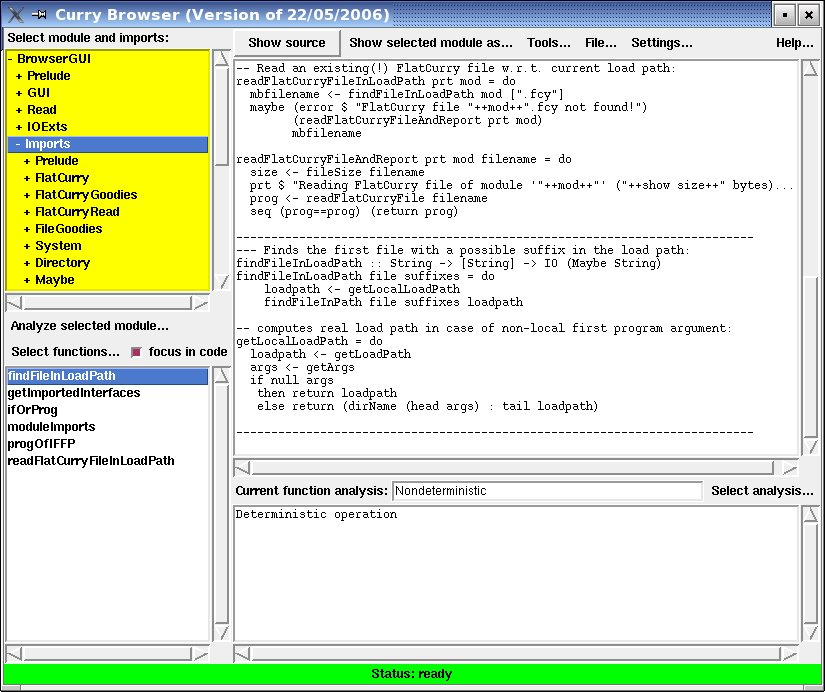
\includegraphics[scale=0.7]{currybrowser.jpg}
\end{center}
\caption{Snapshot of the main window of CurryBrowser\label{fig-currybrowser}}
\end{figure}
%
To get an impression of the use of \cb, Figure~\ref{fig-currybrowser}
shows a snapshot of its use on a particular application
(here: the implementation of \cb).
The upper list box in the left column shows the modules and their imports
in order to browse through the modules of an application.
Similarly to directory browsers, the list of imported modules of a module
can be opened or closed by clicking.
After selecting a module in the list of modules, its source code,
interface, or various other formats of the module can be shown
in the main (right) text area. For instance, one can show
pretty-printed versions of the intermediate flat programs (see below)
in order to see how local function definitions are translated by lambda lifting
\cite{Johnsson85}
or pattern matching is translated into case expressions \cite{Hanus97POPL,Wadler87}.
Since Curry is a language with parametric polymorphism and type inference,
programmers often omit the type signatures when defining functions.
Therefore, one can also view (and store) the selected module as source code where
missing type signatures are added.

Below the list box for selecting modules, there is a menu
(``Analyze selected module'') to analyze all functions
of the currently selected module at once. This is useful
to spot some functions of a module that could be problematic
in some application contexts, like functions that are impure (i.e., the result
depends on the evaluation time) or partially defined (i.e.,
not evaluable on all ground terms).
If such an analysis is selected,
the names of all functions are shown in the
lower list box of the left column (the ``function list'')
with prefixes indicating the properties of the individual functions.

The function list box can be also filled with functions
via the menu ``Select functions''. For instance, all functions
or only the exported functions defined in the currently selected
module can be shown there, or all functions from different modules
that are directly or indirectly called from
a currently selected function.
This list box is central to focus on a function in the
source code of some module or to analyze some function,
i.e., showing their properties. In order to focus on a function,
it is sufficient to check the ``focus on code'' button.
To analyze an individually selected function, one can
select an analysis from the list of available program analyses
(through the menu ``Select analysis'').
In this case, the analysis results are either shown
in the text box below the main text area
or visualized by separate tools, e.g., by a graph drawing tool for
visualizing call graphs.
Some analyses are local, i.e., they need only to consider the local definition
of this function (e.g., ``Calls directly,'' ``Overlapping rules,''
``Pattern completeness''),
where other analyses are global, i.e.,
they consider the definitions of all functions directly or indirectly called
by this function (e.g., ``Depends on,'' ``Solution complete,''
``Set-valued'').
%
Finally, there are a few additional tools integrated into \cb,
for instance, to visualize the import relation between all modules
as a dependency graph. These tools are available through the ``Tools'' menu.

More details about the use of \cb and all built-in analyses
are available through the ``Help'' menu of \cb.


\newpage

\section{CurryTest: A Tool for Testing Curry Programs}
\label{sec-currytest}

CurryTest\index{CurryTest}\index{testing programs}\index{program!testing}
is a simple tool in the PAKCS distribution to write
and run repeatable tests. CurryTest simplifies the task
of writing test cases for a module and executing them.
The tool is easy to use. Assume one has implemented a module \code{MyMod}
and wants to write some test cases to test its functionality,
making regression tests in future versions, etc.
For this purpose, there is a system library \code{Assertion}
(Section~\ref{Library:Assertion}) which
contains the necessary definitions for writing tests.
In particular, it exports an abstract polymorphic type \ccode{Assertion a}
together with the following operations:
\startprog
assertTrue      :: String -> Bool -> Assertion ()
assertEqual     :: String -> a -> a -> Assertion a
assertValues    :: String -> a -> [a] -> Assertion a
assertSolutions :: String -> (a->Success) -> [a] -> Assertion a
assertIO        :: String -> IO a -> a -> Assertion a
assertEqualIO   :: String -> IO a -> IO a -> Assertion a
\stopprog
The expression \ccode{assertTrue $s$ $b$}
is an assertion (named $s$) that the expression $b$ has the value \code{True}.
Similarly, the expression \ccode{assertEqual $s$ $e_1$ $e_2$}
asserts that the expressions $e_1$ and $e_2$
must be equal (i.e., \code{$e_1$==$e_2$} must hold),
the expression \ccode{assertValues $s$ $e$ $vs$} asserts
that $vs$ is the multiset of all values of $e$,
and the expression \ccode{assertSolutions $s$ $c$ $vs$} asserts
that the constraint abstraction $c$ has the multiset of solutions $vs$.
Furthermore, the expression \ccode{assertIO $s$ $a$ $v$}
asserts that the I/O action $a$ yields the value $v$ whenever it is
executed, and
the expression \ccode{assertEqualIO $s$ $a_1$ $a_2$}
asserts that the I/O actions $a_1$ and $a_2$ yields equal values.
The name $s$ provided as a first argument in each assertion
is used in the protocol produced by the test tool.

One can define a test program by importing the module
to be tested together with the module \code{Assertion} and defining
top-level functions of type \code{Assertion} in this module
(which must also be exported).
As an example, consider the following program
that can be used to test some list processing functions:
\startprog
\medskip
import List
import Assertion
\medskip
test1 = assertEqual     "++"     ([1,2]++[3,4]) [1,2,3,4]
\medskip
test2 = assertTrue      "all"    (all (<5) [1,2,3,4])
\medskip
test3 = assertSolutions "prefix" (\labs{}x -> let y free in  x\,++\,y =:= [1,2])
                                 [[],[1],[1,2]]
\medskip
\stopprog
For instance, \code{test1} asserts that the result of evaluating the
expression \code{([1,2]++[3,4])} is equal to \code{[1,2,3,4]}.

We can execute a test suite by the command\pindex{currytest}
\startprog
currytest testList
\stopprog
(\code{currytest} is a program stored in \code{$pakcshome$/bin}
where $pakcshome$ is the installation directory of PAKCS;
see Section~\ref{sec-general}).
In our example, \ccode{testList.curry} is the program containing the
definition of all assertions. This has the effect
that all exported top-level functions
of type \code{Assertion} are tested (i.e., the corresponding
assertions are checked) and the results
(\ccode{OK} or failure) are reported together with the name of each assertion.
%If failures occur, the complete test results are also
%written into a file named \ccode{testList.testlog}.''
For our example above, we obtain the following successful protocol:
\startprog
============================================================
Testing module "testList"...
OK: ++
OK: all
OK: prefix
All tests successfully passed.
============================================================
\stopprog
There is also a graphical interface that summarizes the results
more nicely.\footnote{Due to a bug in older versions of SICStus-Prolog,
it works only with SICStus-Prolog version 3.8.5 (or newer).}
In order to start this interface, one has to add the parameter
\ccode{--window} (or \ccode{-w}), e.g., executing a test suite by
\startprog
currytest --window testList
\stopprog
or
\startprog
currytest -w testList
\stopprog
A snapshot of the interface is shown in Figure~\ref{fig-currytest}.

\begin{figure}%[t]
\begin{center}
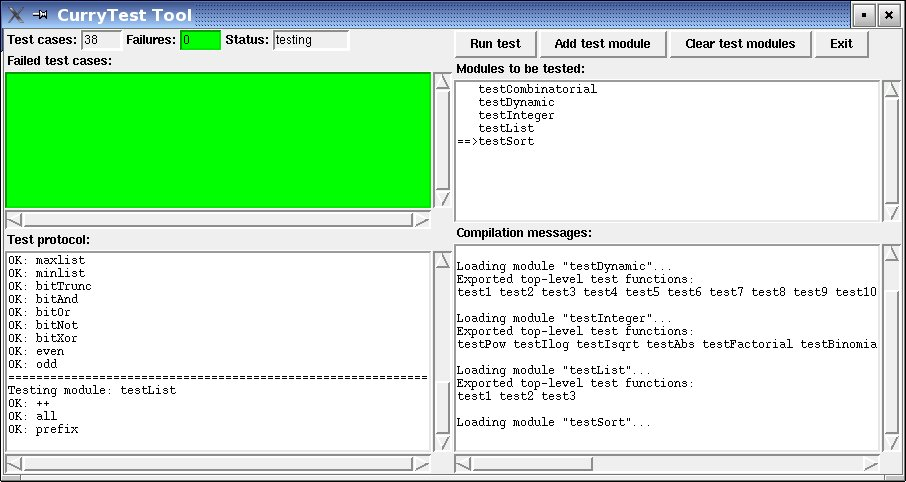
\includegraphics[scale=0.7]{currytest.jpg}
\end{center}
\caption{Snapshot of CurryTest's graphical interface\label{fig-currytest}}
\end{figure}


\newpage

\section{ERD2Curry: A Tool to Generate Programs from ER Specifications}
\label{sec-erd2curry}

ERD2Curry\index{ERD2Curry}\index{database programming}
is a tool to generate Curry code to access and manipulate data
persistently stored from
entity relationship diagrams.\index{entity relationship diagrams}
The idea of this tool is described in detail in
\cite{BrasselHanusMueller08PADL}.
Thus, we describe only the basic steps to use this tool
in the following.

If one creates an entity relationship diagram (ERD)
with the Umbrello UML Modeller, one has to store its
XML description in XMI format (as offered by Umbrello)
in a file, e.g., \ccode{myerd.xmi}.
This description can be compiled into a Curry program by the
command\pindex{erd2curry}
\startprog
erd2curry myerd.xmi
\stopprog
(\code{erd2curry} is a program stored in \code{$pakcshome$/bin}
where $pakcshome$ is the installation directory of PAKCS;
see Section~\ref{sec-general}).
If \code{MyData} is the name of the ERD, the Curry program file
\ccode{MyData.curry} is generated containing all the necessary
database access code as described in \cite{BrasselHanusMueller08PADL}.

If one does not want to use the Umbrello UML Modeller,
one can also create a textual description of the ERD
as a Curry term of type \code{ERD}
(w.r.t.\ the type definition given in module
\code{$pakcshome$/tools/erd2curry/ERD.curry})
and store it in some file, e.g., \ccode{myerd.term}.
This description can be compiled into a Curry program by the
command\pindex{erd2curry}
\startprog
erd2curry -t myerd.term
\stopprog
%
There is also the possibility to visualize an ERD term
as a graph with the graph visualization program \code{dotty}
(for this purpose, it might be necessary to adapt the definition
of the operation \code{dotCmd} in
\code{$pakcshome$/tools/erd2curry/ERD2Graph.curry}
according to your local environment).
This can be done by the command
\startprog
erd2curry -v myerd.term
\stopprog

\paragraph{Inclusion in the Curry application:}
To compile the generated database code, either
include the directory \code{$pakcshome$/tools/erd2curry}
into your Curry load path
(e.g., by setting  the environment variable
\ccode{CURRYPATH}\pindex{CURRYPATH}, see also Section~\ref{sec-modules})
or copy the file
\code{$pakcshome$/tools/erd2curry/ERDGeneric.curry}
into the directory of the generated database code.


\newpage

\section{UI: Declarative Programming of User Interfaces}
\label{sec-ui}

The PAKCS distribution contains a collection of libraries
to implement graphical user interfaces\index{user interface}
as well as web-based user interfaces
from declarative descriptions.
Exploiting these libraries, it is possible
to define the structure and functionality of a user interface
independent from the concrete technology.
Thus, a graphical user interface or a web-based user interface
can be generated from the same description by simply changing
the imported libraries.
This programming technique is described in detail in
\cite{HanusKluss09PADL}.

The libraries implementing these user interfaces are contained
in the directory
\startprog
$pakcshome$/tools/ui
\stopprog
Thus, in order to compile programs containing such user interface
specifications, one has to
include the directory \code{$pakcshome$/tools/ui}
into the Curry load path
(e.g., by setting  the environment variable
\ccode{CURRYPATH}\pindex{CURRYPATH}, see also Section~\ref{sec-modules}).
The directory
\startprog
$pakcshome$/tools/ui/examples
\stopprog
contains a few examples for such user interface specifications.


\newpage

\section{Preprocessing FlatCurry Files}
\label{sec-pakcspp}

The current parser allows to apply transformations on the intermediate
FlatCurry files after they are generated from the
corresponding Curry source file.
Currently, only the FlatCurry file corresponding to the main module
can be transformed.

A transformation can be specified as follows:
\begin{enumerate}
\item {\bf Options to \code{pakcs/bin/parsecurry}:}
\begin{description}
\item[\fbox{\code{--fpopt}}]\pindex{-fpopt}
Apply functional pattern optimization
(see \code{pakcs/tools/optimize/NonStrictOpt.curry} for details).

\item[\fbox{\code{--compact}}]\pindex{--compact}
Apply code compactification after parsing, i.e., transform the main
module and all its imported into one module and delete all
non-accessible functions.

\item[\fbox{\code{--compactexport}}]
Similar to \code{--compact} but delete all functions that are not accessible
from the exported functions of the main module.

\item[\fbox{\code{--compactmain:f}}]
Similar to \code{--compact} but delete all functions that are not accessible
from the function \ccode{f} of the main module.

\item[\fbox{\code{--fcypp cmd}}]\pindex{--fcypp}
Apply command \code{cmd} to the main module after parsing. This is useful to
integrate your own transformation into the compilation process.
Note that the command \ccode{cmd prog} should perform a transformation
on the FlatCurry file \code{prog.fcy}, i.e., it replaces the FlatCurry
file by a new one.
\end{description}

\item {\bf Setting the environment variable \code{FCYPP}:}\pindex{FCYPP}\\
For instance, setting \code{FCYPP} by
\startprog
export FCYPP="--fpopt"
\stopprog
will apply the functional pattern optimization if programs are compiled
and loaded in the PAKCS programming environment.


\item {\bf Putting options into the source code:}\pindex{PAKCS_OPTION_FCYPP}\\
If the source code contains a line with a comment of the form (the comment
must start at the beginning of the line)
\startprog
\{-\# PAKCS_OPTION_FCYPP <options> \#-\}
\stopprog
then the transformations specified by \code{<options>} are applied after
translating the source code into FlatCurry code. For instance,
the functional pattern optimization can be set by the comment
\startprog
\{-\# PAKCS_OPTION_FCYPP --fpopt \#-\}
\stopprog
in the source code. Note that this comment must be in a single line 
of the source program. If there are multiple lines containing such comments,
only the first one will be considered.
\end{enumerate}
\paragraph{Multiple options:}
Note that an arbitrary number of transformations can be specified
by the methods described above.
If several specifications for preprocessing FlatCurry files are used,
they are executed in the following order:
\begin{enumerate}
\item all transformations specified by the environemnt variable
\code{FCYPP} (from left to right)
\item all transformations specified as command line options of parsecurry
   (from left to right)
\item all transformations specified by a comment line in the source code
   (from left to right)
\end{enumerate}


\newpage

\section{Technical Problems}

Due to the fact that Curry is intended to implement
distributed systems (see Appendix~\ref{sec-ports}),
it might be possible that some technical problems
arise due to the use of sockets for implementing these
features. Therefore, this section gives some information
about the technical requirements of PAKCS and how to solve
problems due to these requirements.

There is one fixed port that is used by the implementation of PAKCS:
\begin{description}
\item[Port 8766:] This port is used by the
{\bf Curry Port Name Server} (CPNS) to implement symbolic names for
ports in Curry (see Appendix~\ref{sec-ports}).
If some other process uses this port on the machine,
the distribution facilities defined in the module \code{Ports}
(see Appendix~\ref{sec-ports}) cannot be used.
\end{description}
If these features do not work, you can try to find out
whether this port is in use by the shell command
\ccode{netstat -a | fgrep 8766} (or similar).

The CPNS is implemented as a demon listening on its port 8766
in order to serve requests about registering a new symbolic
name for a Curry port or asking the physical port number
of a Curry port. The demon will be automatically started for
the first time on a machine when a user compiles a program
using Curry ports. It can also be manually started and terminated by the
scripts \code{$pakcshome$/cpns/start} and
\code{$pakcshome$/cpns/stop}.
If the demon is already running, the command \code{$pakcshome$/cpns/start}
does nothing (so it can be always executed
before invoking a Curry program using ports).

If you detect any further technical problem,
please write to
\begin{center}
\code{mh@informatik.uni-kiel.de}
\end{center}

\newpage

\addcontentsline{toc}{section}{Bibliography}
\bibliography{manual}
\bibliographystyle{plain}

\newpage
\appendix

\section{Libraries of the PAKCS Distribution}
\label{sec:libraries}

{\setlength{\parindent}{0.0cm}

The PAKCS compiler system provides an extensive collection
of libraries for application programming.
The libraries for arithmetic constraints over real numbers,
finite domain constraints,
ports for concurrent and distributed programming, and
meta-programming by representing Curry programs in Curry
are described in the following subsection in more detail.
The complete set of libraries with all exported types and functions
are described in the further subsections.
For a more detailed online documentation of all libraries of PAKCS,
see \url{http://www.informatik.uni-kiel.de/~pakcs/lib/index.html}.

\subsection{Constraints, Ports, Meta-Programming}

\subsubsection{Arithmetic Constraints}

The primitive entities for the use of arithmetic constraints
are defined in the system module \code{CLPR}
(cf.\ Section~\ref{sec-modules}), i.e., in order to use them,
the program must contain the import declaration
\startprog
import CLPR
\stopprog
Floating point arithmetic is supported in PAKCS
via arithmetic constraints, i.e., the equational constraint
\ccode{2.3 +.~x =:= 5.5} is solved by binding \code{x} to \code{3.2}
(rather than suspending the evaluation of the addition,
as in corresponding constraints on integers like
\ccode{3+x=:=5}). All operations related to
floating point numbers are suffixed by \ccode{.}.
The following functions and constraints on floating point
numbers are supported in PAKCS:
\begin{description}
\item[\code{(+.)   :: Float -> Float -> Float}]~\\
Addition on floating point numbers.
\item[\code{(-.)   :: Float -> Float -> Float}]~\\
Subtraction on floating point numbers.
\item[\code{(*.)   :: Float -> Float -> Float}]~\\
Multiplication on floating point numbers.
\item[\code{(/.)   :: Float -> Float -> Float}]~\\
Division on floating point numbers.
\item[\code{(<.)   :: Float -> Float -> Success}]~\\
Comparing two floating point numbers with the ``less than'' relation.
\item[\code{(>.)   :: Float -> Float -> Success}]~\\
Comparing two floating point numbers with the ``greater than'' relation.
\item[\code{(<=.)  :: Float -> Float -> Success}]~\\
Comparing two floating point numbers with the ``less than or equal'' relation.
\item[\code{(>=.)  :: Float -> Float -> Success}]~\\
Comparing two floating point numbers with the ``greater than or equal''
relation.
\item[\code{i2f    :: Int -> Float}]~\\
Converting an integer number into a floating point number.
\end{description}
As an example, consider a constraint \code{mortgage}
which relates the principal \code{p},
the lifetime of the mortgage in months \code{t},
the monthly interest rate \code{ir},
the monthly repayment \code{r},
and the outstanding balance at the end of the lifetime \code{b}.
The financial calculations
can be defined by the following two rules in Curry (the second rule
describes the repeated accumulation of the interest):
\startprog
~
import CLPR
~
mortgage p t ir r b | t >. 0.0 \& t <=. 1.0  --lifetime not more than 1 month?
                    =  b =:= p *. (1.0 +. t *. ir) -. t*.r \vspace{1ex}
mortgage p t ir r b | t >. 1.0               --lifetime more than 1 month?
                    =  mortgage (p *. (1.0+.ir)-.r) (t-.1.0) ir r b
~
\stopprog
Then we can calculate the monthly payment for paying back
a loan of \$100,000 in 15 years with a monthly interest rate of 1\%
by solving the goal
\startprog
mortgage 100000.0 180.0 0.01 r 0.0
\stopprog
which yields the solution \code{r=1200.17}.

Note that only linear arithmetic equalities or inequalities
are solved by the constraint solver. Non-linear constraints
like \ccode{x *.~x =:= 4.0} are suspended until they become
linear.


\subsubsection{Finite Domain Constraints}

Finite domain constraints are constraints where all variables
can only take a finite number of possible values.
For simplicity, the domain of finite domain variables are
identified with a subset of the integers, i.e., the type
of a finite domain variable is \code{Int}. The arithmetic
operations related to finite domain variables are suffixed by \ccode{\#}.
The following functions and constraints for finite domain constraint solving
are currently supported in PAKCS:\footnote{Note that
this library is based on the corresponding library of SICStus-Prolog
but does not implement the complete functionality of the SICStus-Prolog library.
However, using the PAKCS interface for external functions (see
Appendix~\ref{sec-external-functions}), it is relatively
easy to provide the complete functionality.}

\begin{description}
\item[\code{domain :: [Int] -> Int -> Int -> Success}]~\\
The constraint \ccode{domain [$x_1,\ldots,x_n$] $l$ $u$}
is satisfied if the domain of all variables $x_i$ is the interval $[l,u]$.
\item[\code{(+\#)   :: Int -> Int -> Int}]~\\
Addition on finite domain values.
\item[\code{(-\#)   :: Int -> Int -> Int}]~\\
Subtraction on finite domain values.
\item[\code{(*\#)   :: Int -> Int -> Int}]~\\
Multiplication on finite domain values.
\item[\code{(=\#)   :: Int -> Int -> Success}]~\\
Equality of finite domain values.
\item[\code{(/=\#)  :: Int -> Int -> Success}]~\\
Disequality of finite domain values.
\item[\code{(<\#)   :: Int -> Int -> Success}]~\\
``less than'' relation on finite domain values.
\item[\code{(<=\#)  :: Int -> Int -> Success}]~\\
``less than or equal'' relation on finite domain values.
\item[\code{(>\#)   :: Int -> Int -> Success}]~\\
``greater than'' relation on finite domain values.
\item[\code{(>=\#)  :: Int -> Int -> Success}]~\\
``greater than or equal'' relation on finite domain values.
\item[\code{sum :: [Int] -> (Int -> Int -> Success) -> Int -> Success}]~\\
The constraint \ccode{sum [$x_1,\ldots,x_n$] $op$ $x$}
is satisfied if all $x_1+\cdots + x_n \mathrel{op} x$ is satisfied,
where $op$ is one of the above finite domain constraint relations
(e.g., \ccode{=\#}).
\item[\code{scalar_product :: [Int] -> [Int] -> (Int -> Int -> Success) -> Int -> Success}]~\\
The constraint \ccode{scalar_product [$c_1,\ldots,c_n$] [$x_1,\ldots,x_n$] $op$ $x$}
is satisfied if all $c_1 x_1+\cdots + c_n x_n \mathrel{op} x$ is satisfied,
where $op$ is one of the above finite domain constraint relations.
\item[\code{count :: Int -> [Int] -> (Int -> Int -> Success) -> Int -> Success}]~\\
The constraint \ccode{count $k$ [$x_1,\ldots,x_n$] $op$ $x$}
is satisfied if all $k \mathrel{op} x$ is satisfied,
where $n$ is the number of the $x_i$ that are equal to $k$ and
$op$ is one of the above finite domain constraint relations.
\item[\code{all_different :: [Int] -> Success}]~\\
The constraint \ccode{all_different [$x_1,\ldots,x_n$]}
is satisfied if all $x_i$ have pairwise different values.
\item[\code{labeling :: [LabelingOption] -> [Int] -> Success}]~\\
The constraint \ccode{labeling $os$ [$x_1,\ldots,x_n$]}
non-deterministically instantiates all $x_i$ to the values
of their domain according to the options $os$ (see the module documentation
for further details about these options).
\end{description}
These entities are defined in the system module \code{CLPFD}
(cf.\ Section~\ref{sec-modules}), i.e., in order to use it,
the program must contain the import declaration
\startprog
import CLPFD
\stopprog
As an example, consider the classical \ccode{send+more=money} problem
where each letter must be replaced by a different digit such that this
equation is valid and there are no leading zeros.
The usual way to solve finite domain constraint problems
is to specify the domain of the involved variables followed
by a specification of the constraints and the labeling
of the constraint variables in order to start the search for solutions.
Thus, the \ccode{send+more=money} problem can be solved as follows:
\startprog
~
import CLPFD
~
smm l =
        l =:= [s,e,n,d,m,o,r,y] \&
        domain l 0 9 \&
        s >\# 0 \&
        m >\# 0 \&
        all_different l  \&
                         1000 *\# s +\# 100 *\# e +\# 10 *\# n +\# d
        +\#               1000 *\# m +\# 100 *\# o +\# 10 *\# r +\# e
        =\# 10000 *\# m +\# 1000 *\# o +\# 100 *\# n +\# 10 *\# e +\# y \&
        labeling [FirstFail] l
        where s,e,n,d,m,o,r,y free
~
\stopprog
Then we can solve this problem by evaluating the goal
\ccode{smm [s,e,n,d,m,o,r,y]} which yields the unique solution
\code{\{s=9,e=5,n=6,d=7,m=1,o=0,r=8,y=2\}}.


\subsubsection{Ports: Distributed Programming in Curry}
\label{sec-ports}

To support the development of concurrent and distributed applications,
PAKCS supports internal and external ports\index{ports} as
described in \cite{Hanus99PPDP}.
Since \cite{Hanus99PPDP} contains a detailed description of this
concept together with various programming examples, we only summarize here
the functions and constraints supported for ports in PAKCS.

The basic datatypes, functions, and constraints for ports
are defined in the system module \code{Ports}
(cf.\ Section~\ref{sec-modules}), i.e., in order to use ports,
the program must contain the import declaration
\startprog
import Ports
\stopprog
This declaration includes the following entities in the program:
\begin{description}
\item[\code{Port a}\pindex{Port}]~\\
This is the datatype of a port to which one can send messages of type \code{a}.

\item[\code{openPort :: Port a -> [a] -> Success}]~\\
The constraint \ccode{openPort p s}\pindex{openPort}
establishes a new \emph{internal port}
\code{p} with an associated message stream \code{s}. \code{p} and \code{s} must be
unbound variables,
otherwise the constraint fails (and causes a runtime error).

\item[\code{send :: a -> Port a -> Success}]~\\
The constraint \ccode{send m p}\pindex{send}
is satisfied if \code{p} is constrained
to contain the message \code{m}, i.e., \code{m} will be sent to the port
\code{p} so that it appears in the corresponding stream.

\item[\code{doSend :: a -> Port a -> IO ()}]~\\
The I/O action \ccode{doSend m p}\pindex{doSend} solves the constraint
\ccode{send m p} and returns nothing.

\item[\code{openNamedPort :: String -> IO [a]}]~\\
The I/O action \ccode{openNamedPort n}\pindex{openNamedPort}
opens a new \emph{external port} with
symbolic name \code{n} and returns the associated stream of messages.

\item[\code{connectPort :: String -> IO (Port a)}]~\\
The I/O action \ccode{connectPort n}\pindex{connectPort}
returns a port with symbolic name
\code{n} (i.e., \code{n} must have the form ``\emph{portname@machine})
to which one can send messages by the \code{send} constraint.
Currently, no dynamic type checking is done for external ports,
i.e., sending messages of the wrong type to a port might lead to
a failure of the receiver.
\end{description}

\paragraph{Restrictions:}
Every expression, possibly containing logical variables, can be sent to
a port. However, as discussed in \cite{Hanus99PPDP},
port communication is strict, i.e., the expression is
evaluated to normal form before sending it by the
constraint \code{send}. Furthermore, if messages containing
logical variables are sent to \emph{external ports},
the behavior is as follows:
\begin{enumerate}
\item The sender waits until all logical variables in the message
have been bound by the receiver.
\item The binding of a logical variable received by a process
is sent back to the sender of this logical variable only if
it is bound to a \emph{ground} term, i.e., as long as the binding contains
logical variables, the sender is not informed about the binding
and, therefore, the sender waits.
\end{enumerate}

\paragraph{External ports on local machines:}
The implementation of external ports assumes that the
host machine running the application is connected to the Internet
(i.e., it uses the standard IP address of the host machine
for message sending). If this is not the case and the application
should be tested by using external ports only on the local host
without a connection to the Internet,
the environment variable \ccode{PAKCS_LOCALHOST}\pindex{PAKCS_LOCALHOST}
must be set to \ccode{yes}
\emph{before PAKCS system is started}.
In this case, the IP address \code{127.0.0.1} and the hostname
\ccode{localhost} are used for identifying the local machine.

\paragraph{Selection of Unix sockets for external ports:}
The implementation of ports uses sockets to communicate
messages sent to external ports.
Thus, if a Curry program uses the
I/O action \code{openNamedPort}\pindex{openNamedPort}
to establish an externally visible server,
PAKCS selects a Unix socket for the port communication.
Usually, a free socket is selected by the operating system.
If the socket number should be fixed in an application (e.g.,
because of the use of firewalls\index{firewall} that allow only
communication over particular sockets), then one
can set the environment variable \ccode{PAKCS_SOCKET}\pindex{PAKCS_SOCKET}
to a distinguished socket number before the PAKCS system is started.
This has the effect that PAKCS uses only this socket
number for communication (even for several external ports
used in the same application program).

\paragraph{Debugging:}
To debug distributed systems,
it is sometimes helpful to see all messages sent to external ports.
This is supported by the environment variable
\ccode{PAKCS_TRACEPORTS}.\pindex{PAKCS_TRACEPORTS}
If this variable is set to \ccode{yes}
\emph{before the PAKCS system is started}, then all
connections to external ports and all
messages sent and received on external ports are
printed on the standard error stream.


\subsubsection{AbstractCurry and FlatCurry: Meta-Programming in Curry}
\label{sec-flatcurry}

\index{AbstractCurry}
\index{FlatCurry}
To support meta-programming, i.e., the manipulation of Curry programs
in Curry, there are system modules \code{FlatCurry} and \code{AbstractCurry}
(stored in the directory \ccode{$pakcshome$/lib/meta})
which define datatypes for the representation
of Curry programs.
\code{AbstractCurry} is a more direct representation of a Curry program,
whereas \code{FlatCurry} is a simplified representation
where local function definitions are replaced by global definitions
(i.e., lambda lifting has been performed) and pattern matching
is translated into explicit case/or expressions.
Thus, \code{FlatCurry} can be used for more back-end oriented
program manipulations (or, for writing new back ends for Curry),
whereas \code{AbstractCurry} is intended for manipulations of
programs that are more oriented towards the source program.

Both modules contain predefined I/O actions to read programs
in the \code{AbstractCurry} (\code{readCurry}\pindex{readCurry})
or \code{FlatCurry}
(\code{readFlatCurry}\pindex{readFlatCurry}) format.
These actions parse the corresponding source program and return
a data term representing this program (according to the definitions
in the modules \code{AbstractCurry} and \code{FlatCurry}).

Since all datatypes are explained in detail in these modules,
we refer to the online documentation\footnote{%
\url{http://www.informatik.uni-kiel.de/~pakcs/lib/CDOC/FlatCurry.html} and
\url{http://www.informatik.uni-kiel.de/~pakcs/lib/CDOC/AbstractCurry.html}}
of these modules.

As an example, consider a program file \ccode{test.curry}
containing the following two lines:
\startprog
rev []     = []
rev (x:xs) = (rev xs) ++ [x]
\stopprog
Then the I/O action \code{(FlatCurry.readFlatCurry "test")} returns the
following term:
\startprog
 (Prog "test"
  ["Prelude"]
  []
  [Func ("test","rev") 1 Public
        (FuncType (TCons ("Prelude","[]") [(TVar 0)])
                  (TCons ("Prelude","[]") [(TVar 0)]))
        (Rule [0]
           (Case Flex (Var 0)
              [Branch (Pattern ("Prelude","[]") [])
                  (Comb ConsCall ("Prelude","[]") []),
               Branch (Pattern ("Prelude",":") [1,2])
                  (Comb FuncCall ("Prelude","++")
                        [Comb FuncCall ("test","rev") [Var 2],
                         Comb ConsCall ("Prelude",":")
                              [Var 1,Comb ConsCall ("Prelude","[]") []]
                        ])
              ]))]
  []
 )
\stopprog


%%%%%%%%%%%%%%%%%%%%%%%%%%%%%%%%%%%%%%%%%%%%%%%%%%%%%%%%%%%%%%%%%%%%%%%%%
% Definitions in order to LaTeX documents generated by "currydoc --tex"
%%%%%%%%%%%%%%%%%%%%%%%%%%%%%%%%%%%%%%%%%%%%%%%%%%%%%%%%%%%%%%%%%%%%%%%%%

\newcommand{\currymodule}[1]{\subsubsection{Library #1}\label{Library:#1}}
\newcommand{\currytypesstart}{\subsubsection*{Exported types:}}
\newcommand{\currytypesstop}{}
\newcommand{\currytypesynstart}[2]{{\tt type #2}\pindex{#1} \begin{quote}}
\newcommand{\currytypesynstop}{\end{quote}}
\newcommand{\currydatastart}[1]{{\tt data #1}\pindex{#1} \begin{quote}}
\newcommand{\currydatacons}{\end{quote}%
\begin{itemize}\item[] \hspace{-4ex}\emph{Exported constructors:}}
\newcommand{\currydatastop}{\end{itemize}}
\newcommand{\curryconsstart}[2]{\item {\tt #1~::~#2}\par}
\newcommand{\curryfuncstart}{\subsubsection*{Exported functions:}}
\newcommand{\curryfuncstop}{}
\newcommand{\curryfunctionstart}[2]{#2\pindex{#1}\begin{quote}}
\newcommand{\curryfunctionstop}{\end{quote}}
\newcommand{\curryfuncsig}[2]{{\tt #1~::~#2}}


\subsection{General Libraries}

\input{lib/AllSolutions}
\input{lib/Assertion}
\input{lib/Char}
\input{lib/CLPFD}
\input{lib/CLPR}
\input{lib/CLPB}
\input{lib/Combinatorial}
\input{lib/Constraint}
\input{lib/CSV}
\input{lib/Database}
\input{lib/DaVinci}
\input{lib/Directory}
\input{lib/Dynamic}
\input{lib/FileGoodies}
\input{lib/Float}
\input{lib/Global}
\input{lib/GlobalVariable}
\input{lib/GUI}
\input{lib/Integer}
\input{lib/IO}
\input{lib/IOExts}
\input{lib/JavaScript}
\input{lib/KeyDatabase}
\input{lib/KeyDatabaseSQLite}
\input{lib/KeyDB}
\input{lib/List}
\input{lib/Maybe}
\input{lib/NamedSocket}
\input{lib/Parser}
\input{lib/Ports}
\input{lib/Pretty}
\input{lib/Profile}
\input{lib/PropertyFile}
\input{lib/Read}
\input{lib/ReadNumeric}
\input{lib/ReadShowTerm}
\input{lib/SetFunctions}
\input{lib/Socket}
\input{lib/System}
\input{lib/Time}
%\input{lib/Tk}
\input{lib/Unsafe}


\subsection{Data Structures and Algorithms}

\input{lib/Array}
\input{lib/Dequeue}
\input{lib/FiniteMap}
\input{lib/GraphInductive}
\input{lib/Random}
\input{lib/RedBlackTree}
\input{lib/SetRBT}
\input{lib/Sort}
\input{lib/TableRBT}
\input{lib/Traversal}

\subsection{Libraries for Web Applications}

\input{lib/CategorizedHtmlList}
\input{lib/HTML}
\input{lib/HtmlParser}
\input{lib/Mail}
\input{lib/Markdown}
\input{lib/WUI}
\input{lib/URL}
\input{lib/XML}
\input{lib/XmlConv}

\subsection{Libraries for Meta-Programming}

\input{lib/AbstractCurry}
\input{lib/AbstractCurryPrinter}
\input{lib/CompactFlatCurry}
\input{lib/CurryStringClassifier}
\input{lib/FlatCurry}
\input{lib/FlatCurryGoodies}
\input{lib/FlatCurryRead}
\input{lib/FlatCurryShow}
\input{lib/FlatCurryTools}
\input{lib/FlatCurryXML}
\input{lib/FlexRigid}
\input{lib/PrettyAbstract}

} % end setlength parindent

\newpage

\input{markdown_syntax}

\newpage

\begin{figure}%[t]
\begin{center}
 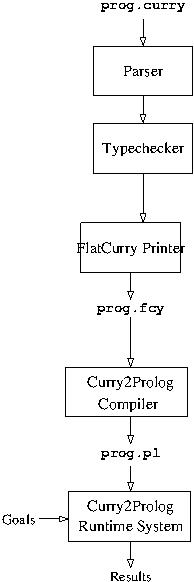
\includegraphics[scale=0.85]{pakcs_overview.jpg}
\end{center}\vspace{-5ex}
\caption{Overview of PAKCS\label{fig-pakcs}}
\end{figure}

\section{Overview of the PAKCS Distribution}

A schematic overview of the various components contained in
the distribution of PAKCS and the
translation process of programs inside PAKCS is shown in
Figure~\ref{fig-pakcs} on page~\pageref{fig-pakcs}.
In this figure, boxes denote different components of PAKCS
and names in boldface denote files containing
various intermediate representations during the translation
process (see Section~\ref{sec-auxfiles} below).
The PAKCS distribution contains a front end for reading (parsing and
type checking) Curry programs that can be also used by
other Curry implementations.
The back end (formerly known as ``Curry2Prolog''\index{Curry2Prolog})
compiles Curry programs into Prolog programs.
It also support constraint solvers for
arithmetic constraints over real numbers and finite domain constraints,
and further libraries for GUI programming, meta-programming etc.
Currently, it does not implement encapsulated search in full generality
(only a strict version of \code{findall} is supported),
and concurrent threads are not executed in a fair manner.


\newpage

\section{Auxiliary Files}
\label{sec-auxfiles}

During the translation and execution of a Curry program with PAKCS,
various intermediate representations of the source program are created
and stored in different files which are shortly explained in this section.
If you use the PAKCS, it is not necessary to know about
these auxiliary files because they are automatically generated
and updated. You should only remember the command for deleting
all auxiliary files (\ccode{cleancurry}, see Section~\ref{sec-general})
to clean up your directories.

The various components of PAKCS create
the following auxiliary files.
\begin{description}
\item[\code{prog.fcy}:] This file contains the Curry program
in the so-called ``FlatCurry'' representation where all functions are global
(i.e., lambda lifting has been performed) and pattern matching
is translated into explicit case/or expressions
(compare Appendix~\ref{sec-flatcurry}).
This representation might be useful for other back ends and
compilers for Curry and is the basis doing meta-programming in Curry.
This file is implicitly
generated when a program is read by PAKCS.
It can be also explicitly generated by the command\pindex{parsecurry}
\startprog
parsecurry --flat prog
\stopprog
The FlatCurry representation of a Curry program is usually
generated by the front-end after parsing, type checking and eliminating
local declarations.
If $dir$ is the directory where the Curry program is stored,
the corresponding FlatCurry program is stored in the directory
\ccode{$dir$/.curry}.

\item[\code{prog.fint}:] This file contains the interface
of the program in the so-called ``FlatCurry'' representation,
i.e., it is similar to \code{prog.fcy} but contains only exported
entities and the bodies of all functions omitted (i.e., ``external'').
This representation is useful for providing a fast access
to module interfaces.
This file is implicitly generated by the command\pindex{parsecurry}
\startprog
parsecurry --flat prog
\stopprog
and stored in the same directory as \code{prog.fcy}.

\item[\code{prog.pl}:] This file contains a Prolog program
as the result of translating the Curry program with PAKCS.
If $dir$ is the directory where the Curry program is stored,
the corresponding Prolog program is stored in the directory
\ccode{$dir$/.curry/.pakcs}.

\item[\code{prog.po}:] This file contains the Prolog program
\code{prog.pl} in an intermediate format for faster loading.
This file is stored in the same directory as \code{prog.pl}.

\item[\code{prog.state}:] This file contains the saved state
after compiling and saving a program with PAKCS
(see Section~\ref{sec-use-curry2prolog}).

\end{description}


\newpage


\section{Changing the Prelude or System Modules}

The standard prelude, which is automatically imported into each Curry program,
and all system modules containing datatypes and functions
useful for application programming
(cf.\ Appendix~\ref{sec:libraries})
are stored in the system module directory \ccode{$pakcshome$/lib}
(and its subdirectories).
If you change any of these modules,
you have to recompile the complete system by
executing \code{make} in the directory $pakcshome$.



\newpage

\section{External Functions}
\label{sec-external-functions}

\index{function!external}\index{external function}
Currently, PAKCS has no general interface to external functions.
Therefore, if a new external function should be added
to the system, this function must be declared as \code{external}
in the Curry source code
and then an implementation for this external function
must be inserted in the corresponding back end.
An external function is defined as follows in the Curry source code:
\begin{enumerate}
\item
Add a type declaration for the external function somewhere
in the body of the appropriate file (usually, the prelude
or some system module).
\item
For external functions it is not allowed to define any
rule since their semantics is determined by an external implementation.
Instead of the defining rules, you have to write
\startprog
f external
\stopprog
somewhere in the file containing the type declaration for 
the external function \code{f}.
\end{enumerate}
For instance, the addition on integers can be declared as
an external function as follows:
\startprog
(+) :: Int -> Int -> Int
(+) external
\stopprog
The further modifications to be done for an inclusion of
an external function has to be done in the back end.
A new external function is added to the back end of PAKCS
by informing the compiler about the existence of an external function
and adding an implementation of this function in the run-time
system. Therefore, the following items must be added
in the PAKCS compiler system:
\begin{enumerate}
\item
If the Curry module \code{Mod} contains external functions,
there must be a file named \code{Mod.prim_c2p} containing the
specification of these external functions. The contents of this file
is in XML format and has the following general structure:\footnote{%
\url{http://www.informatik.uni-kiel.de/~pakcs/primitives.dtd} contains a DTD
describing the exact structure of these files.}
\startprog
<primitives>
  \emph{specification of external function $f_1$}
  \ldots
  \emph{specification of external function $f_n$}
</primitives>
\stopprog
The specification of an external function $f$
with arity $n$ has the form
\startprog
<primitive name="$f$" arity="$n$">
  <library>lib</library>
  <entry>pred</entry>
</primitive>
\stopprog
where \code{lib} is the Prolog library (stored in the directory of the
Curry module or in the global directory
\code{$pakcshome$/curry2prolog/lib_src}) containing the code implementing this
function and \code{pred} is a predicate name in this library
implementing this function. Note that the function $f$ must be
declared in module \code{Mod}: either as an external function
or defined in Curry by equations. In the latter case,
the Curry definition is not translated but calls to this function
are redirected to the Prolog code specified above.

Furthermore, the list of specifications can also contain entries of the form
\startprog
<ignore name="$f$" arity="$n$" />
\stopprog
for functions $f$ with arity $n$ that are declared in module \code{Mod}
but should be ignored for code generation, e.g., since they are
never called w.r.t.\ to the current implementation of external functions.
For instance, this is useful when functions that can
be defined in Curry should be (usually more efficiently) are implemented
as external functions.

Note that the arguments are passed in their current (possibly unevaluated) form.
Thus, if the external function requires the arguments to be evaluated
in a particular form, this must be done before calling the external function.
For instance, the external function for adding two integers
requires that both arguments must be evaluated to non-variable head normal form
(which is identical to the ground constructor normal form). Therefore,
the function \ccode{+} is specified in the prelude by
\startprog
(+)   :: Int -> Int -> Int
x + y = (prim_Int_plus \$\# y) \$\# x
\medskip
prim_Int_plus :: Int -> Int -> Int
prim_Int_plus external
\stopprog
where \code{prim_Int_plus} is the actual external function implementing
the addition on integers. Consequently, the specification file
\code{Prelude.prim_c2p} has an entry of the form
\startprog
<primitive name="prim_Int_plus" arity="2">
  <library>prim_standard</library>
  <entry>prim_Int_plus</entry>
</primitive>
\stopprog
where the Prolog library \code{prim_standard.pl} contains the Prolog code
implementing this function.

\item
For most external functions, a \emph{standard interface} is
generated by the compiler so that an $n$-ary function can be
implemented by an $(n+1)$-ary predicate where the last argument must
be instantiated to the result of evaluating the function.  The
standard interface can be used if all arguments are ensured to be
fully evaluated (e.g., see definition of \code{(+)} above) and no
suspension control is necessary, i.e., it is ensured that the
external function call does not suspend for all arguments.
Otherwise, the raw interface (see below) must be used.  For
instance, the Prolog code implementing \code{prim_Int_plus}
contained in the Prolog library \code{prim_standard.pl} is as
follows (note that the arguments of \code{(+)} are passed in reverse
order to \code{prim_Int_plus} in order to ensure a left-to-right
evaluation of the original arguments by the calls to \code{(\$\#)}):
\startprog
prim_Int_plus(Y,X,R) :- R is X+Y.
\stopprog

\item
The \emph{standard interface for I/O actions}, i.e., external functions
with result type \code{IO~a}, assumes that the I/O action
is implemented as a predicate (with a possible side effect)
that instantiates the last argument to the returned value of type \ccode{a}.
For instance, the primitive predicate \code{prim_getChar}
implementing prelude I/O action \code{getChar}
can be implemented by the Prolog code
\startprog
prim_getChar(C) :- get_code(N), char_int(C,N).
\stopprog
where \code{char_int} is a predicate relating the internal
Curry representation of a character with its ASCII value.

\item
If some arguments passed to the external functions are not fully evaluated
or the external function might suspend, the implementation must follow
the structure of the PAKCS run-time system by using
the \emph{raw interface}. In this case, the name of the external entry
must be suffixed by \ccode{[raw]} in the \code{prim_c2p} file.
For instance, if we want to use the raw interface for the external function
\code{prim_Int_plus},
the specification file \code{Prelude.prim_c2p} must have an entry of the form
\startprog
<primitive name="prim_Int_plus" arity="2">
  <library>prim_standard</library>
  <entry>prim_Int_plus[raw]</entry>
</primitive>
\stopprog
In the raw interface, the actual implementation of an $n$-ary external function consists
of the definition of an $(n+3)$-ary predicate $pred$.
The first $n$ arguments are the corresponding actual arguments.
The $(n+1)$-th argument is a free variable which must be
instantiated to the result of the function call after
successful execution. The last two arguments
control the suspension behavior of the function
(see \cite{AntoyHanus00FROCOS} for more details):
The code for the predicate $pred$
should only be executed when the $(n+2)$-th argument
is not free, i.e., this predicate has always the
SICStus-Prolog block declaration
\startprog
?- block $pred$(?,\ldots,?,-,?).
\stopprog
In addition, typical external functions should suspend
until the actual arguments are instantiated. This can be ensured
by a call to \code{ensureNotFree} or \code{(\$\#)}
before calling the external function. Finally, the
last argument (which is a free variable at call time)
must be unified with the $(n+2)$-th argument
after the function call is successfully evaluated
(and does not suspend). Additionally, the actual (evaluated) arguments
must be dereferenced before they are accessed.
Thus, an implementation
of the external function for adding integers is as follows in the raw interface:
\startprog
?- block prim_Int_plus(?,?,?,-,?).
prim_Int_plus(RY,RX,Result,E0,E) :-
     deref(RX,X), deref(RY,Y), Result is X+Y, E0=E.
\stopprog
Here, \code{deref} is a predefined predicate for dereferencing the
actual argument into a constant (and \code{derefAll} for dereferencing
complex structures).
\end{enumerate}
%
The Prolog code implementing the external functions must be accessible to the run-time
system of PAKCS by putting it into the directory containing the corresponding
Curry module or into the system directory
\code{$pakcshome$/curry2prolog/lib_src}.
Then it will be automatically loaded into the run-time environment
of each compiled Curry program.

Note that arbitrary functions implemented in C or Java can be connected to
PAKCS by using the corresponding interfaces of underlying Prolog system.


\newpage
\addcontentsline{toc}{section}{Index}
\printindex


\end{document}

\clearpage
\documentclass[11pt,fleqn]{article}

\usepackage{latexsym}
\usepackage{makeidx}
\usepackage{url}
\usepackage{xspace}
\usepackage{graphicx}

\input{version}

%%% ------------------------------------------------------------------

\usepackage[colorlinks,linkcolor=blue]{hyperref}
\hypersetup{bookmarksopen=true}
\hypersetup{bookmarksopenlevel=0}
\hypersetup{pdftitle={PAKCS: The Portland Aachen Kiel Curry System}}
\hypersetup{pdfauthor={Michael Hanus}}
%\hypersetup{pdfstartview=Title}
\hypersetup{pdfstartview=FitH}
\usepackage{thumbpdf}

%%% ------------------------------------------------------------------

\setlength{\textwidth}{16.5cm}
\setlength{\textheight}{23cm}
\renewcommand{\baselinestretch}{1.1}
\setlength{\topmargin}{-1cm}
\setlength{\oddsidemargin}{0cm}
\setlength{\evensidemargin}{0cm}
\setlength{\marginparwidth}{0.0cm}
\setlength{\marginparsep}{0.0cm}

\newlength{\figurewidth}
\setlength{\figurewidth}{\textwidth}
\addtolength{\figurewidth}{-0.4cm}

% font for program texts
\renewcommand{\tt}{\usefont{OT1}{cmtt}{m}{n}\selectfont}
\newcommand{\codefont}{\tt}

% environment for typing program texts:
\makeatletter
\newenvironment{prog}{\par\vspace{0.7ex}
\setlength{\parindent}{1.0cm}
\setlength{\parskip}{-0.1ex}
\obeylines\@vobeyspaces\tt}{\vspace{0.7ex}\noindent
}
\makeatother
\newcommand{\startprog}{\begin{prog}}
\newcommand{\stopprog}{\end{prog}\noindent}

% program text in normal text
\newcommand{\code}[1]{\mbox{\codefont #1}}

% program text in normal text with apostrophs
\newcommand{\ccode}[1]{``\mbox{\codefont #1}''}

\newcommand{\pindex}[1]{\index{#1@{\tt #1}}}  % program elements in index

\newcommand{\labs}{\mbox{\tt\char92}}  % lambda abstraction in Curry
\newcommand{\todo}[1]{\fbox{\sc To do: #1}}
\newcommand{\cb}{CurryBrowser\xspace}

% allow underscores in programs:
\catcode`\_=\active
\let_=\sb
\catcode`\_=12

% produce an index:
\makeindex

\begin{document}
\sloppy

\begin{titlepage}
\pdfbookmark[1]{Title}{Title}
\begin{center}
\fbox{
\begin{minipage}[t]{\figurewidth}
\begin{center}\vspace{10ex}
{\Huge\bf PAKCS \pakcsversion}\\[4ex]
{\huge The Portland Aachen Kiel Curry System}\\[7ex]
{\huge User Manual}\\[4ex]
\pakcsversiondate\\[6ex]
\Large
Michael Hanus$^1$ [editor] \\[3ex]
{\large Additional Contributors:}\\[2ex]
Sergio Antoy$^2$ \\
Bernd Bra\ss{}el$^3$ \\
Martin Engelke$^4$ \\
Klaus H\"oppner$^5$ \\
Johannes Koj$^6$ \\
Philipp Niederau$^7$ \\
Ramin Sadre$^8$ \\
Frank Steiner$^9$ \\[4ex]
\normalsize
(1) University of Kiel, Germany, {\tt mh@informatik.uni-kiel.de} \\
(2) Portland State University, USA, {\tt antoy@cs.pdx.edu} \\
(3) University of Kiel, Germany, {\tt bbr@informatik.uni-kiel.de} \\
(4) University of Kiel, Germany, {\tt men@informatik.uni-kiel.de} \\
(5) University of Kiel, Germany, {\tt klh@informatik.uni-kiel.de} \\
(6) RWTH Aachen, Germany, {\tt johannes.koj@sdm.de} \\
(7) RWTH Aachen, Germany, {\tt philipp@navigium.de} \\
(8) RWTH Aachen, Germany, {\tt ramin@lvs.informatik.rwth-aachen.de} \\
(9) LMU Munich, Germany, {\tt fst@bio.informatik.uni-muenchen.de} \\[5ex]~
\end{center}
\end{minipage}}
\end{center}
\end{titlepage}

\pdfbookmark[1]{Contents}{Contents}
\tableofcontents

\newpage

\addcontentsline{toc}{section}{Preface}
\section*{Preface}

This document describes PAKCS (formerly called ``PACS''),
an implementation of the multi-paradigm language Curry,
jointly developed at the University of Kiel, the Technical University
of Aachen and Portland State University.
Curry is a universal programming language aiming at the amalgamation
of the most important declarative programming paradigms,
namely functional programming and logic programming.  
Curry combines in a seamless way features from functional programming
(nested expressions, lazy evaluation, higher-order functions),
logic programming (logical variables, partial data structures,
built-in search), and concurrent programming (concurrent evaluation
of constraints with synchronization on logical variables).
Moreover, the PAKCS implementation of Curry also supports
the high-level implementation of distributed applications,
graphical user interfaces, and web services
(as described in more detail in \cite{Hanus99PPDP,Hanus00PADL,Hanus01PADL}).

We assume familiarity with the ideas and features
of Curry as described in the Curry language definition \cite{Hanus12Curry}.
Therefore, this document only explains the use of the different
components of PAKCS
and the differences and restrictions of PAKCS
(see Section~\ref{sec-restrictions})
compared with the language Curry (Version 0.8.3).


\bigskip

\subsection*{Acknowledgements}

This work has been supported in part by the DAAD/NSF grant INT-9981317,
the NSF grants CCR-0110496 and CCR-0218224,
the Acci\'on Integrada hispano-alemana HA1997-0073,
and the DFG grants Ha 2457/1-2, Ha 2457/5-1, and Ha 2457/5-2.

Many thanks to the users of PAKCS for bug reports, bug fixes, and improvements,
in particular, to Marco Comini, Sebastian Fischer, Massimo Forni,
Carsten Heine, Stefan Junge, Frank Huch, Parissa Sadeghi.


\newpage

\section{Overview of PAKCS}

\subsection{General Use}
\label{sec-general}

This version of PAKCS has been tested on Sun Solaris, Linux, and Mac OS X
systems. In principle, it should be also executable on other
platforms on which a Prolog system like SICStus-Prolog or SWI-Prolog exists
(see the file \code{INSTALL.html} in the PAKCS directory
for a description of the necessary software to install PAKCS).

All executable files required to use the different components
of PAKCS are stored in the directory \code{$pakcshome$/bin}
(where $pakcshome$ is the installation directory of the complete
PAKCS installation). You should add this directory
to your path (e.g., by the \code{bash} command
\ccode{export PATH=$pakcshome$/bin:\$PATH}).

The source code of the Curry program
must be stored in a file with the suffix \ccode{.curry},
e.g., \code{prog.curry}. 
Literate programs must be stored in files with the extension \ccode{.lcurry}.
They are automatically converted into corresponding
\ccode{.curry} files by deleting all lines not starting 
with \ccode{>} and removing the prefix \ccode{> } of the
remaining lines.

Since the translation of Curry programs with PAKCS creates
some auxiliary files (see Section~\ref{sec-auxfiles} for details),
you need write permission
in the directory where you have stored your Curry programs.
The auxiliary files for all Curry programs in the current
directory can be deleted by the command\pindex{cleancurry}
\startprog
cleancurry
\stopprog
(this is a shell script stored in the \code{bin} directory of the
PAKCS installation, see above).
The command
\startprog
cleancurry -r
\stopprog
also deletes the auxiliary files in all subdirectories.



\subsection{Restrictions on Curry Programs}
\label{sec-restrictions}

There are a few minor restrictions on Curry programs
when they are processed with PAKCS:
\begin{itemize}
\item
\index{singleton variables}\index{variables!singleton}
\emph{Singleton pattern variables}, i.e., variables that occur only once
in a pattern of the rule, should be denoted as an anonymous variable \ccode{_},
otherwise the parser will print a warning since this is a
typical source of programming errors.
\item
PAKCS translates all \emph{local declarations} into global functions with
additional arguments (``lambda lifting'', see Appendix~D of the
Curry language report).
Thus, in the various run-time systems, the definition of
functions with local declarations look different from
their original definition (in order to see the result
of this transformation, you can use the \cb, see
Section~\ref{sec-currybrowser}).
\item \index{tabulator stops}
Tabulator stops instead of blank spaces in source files are
interpreted as stops at columns 9, 17, 25, 33, and so on.
\item Threads created by a concurrent conjunction are not executed
in a fair manner (usually, threads corresponding to leftmost constraints
are executed with higher priority).
\item
Encapsulated search\index{encapsulated search}: In order
to allow the integration of non-deterministic computations
in programs performing I/O at the top-level, PAKCS supports
the search operators \code{findall}\pindex{findall}
and \code{findfirst}\pindex{findfirst}.
In contrast to the general definition of encapsulated search
\cite{HanusSteiner98PLILP}, the current implementation suspends
the evaluation of \code{findall} and \code{findfirst}
until the argument does not contain unbound global variables.
Moreover, the evaluation of \code{findall} is strict,
i.e., it computes all solutions before returning the
complete list of solutions.
It is recommended to use the system module \code{AllSolutions}
for encapsulating search.
\item
There is currently no general connection to external constraint solvers.
However, the PAKCS compiler provides constraint
solvers for arithmetic and finite domain constraints
(see Appendix~\ref{sec:libraries}).
\end{itemize}

% Layout rule:
% (from Sergio's email of June 2, 1998)
%This is the general rule.  There are two kinds of syntactic
%constructs that rely on the offside rule.  One kind has a keyword
%indicating the end of the construct.  "let ... in" is the only
%representative of this kind.  Upon recognition of the keyword
%"in", all the constructs relying on the offide rule nested within
%the "let...in" are closed.  The other kind has no closing keyword.
%"where" and "choice" are the only constructs of this kind.
%Constructs of this kind can be closed only by indentation.  Any
%line, including a comment, indented less that the construct
%terminates it.  The indentation of "where", "choice" and "let" is
%the indentation of the first token following the keyword of the
%construct.
%



\subsection{Modules in PAKCS}
\label{sec-modules}

The current implementation of PAKCS supports only flat module names,
i.e., the notation \code{Dir.Mod.f} is not supported.\index{modules}
In order to allow the structuring of modules in different directories,
PAKCS searches for imported modules in various directories.
By default, imported modules are searched in the directory
of the main program and the system module directories
\ccode{$pakcshome$/lib} and \ccode{$pakcshome$/lib/meta}.
This search path can be extended
by setting the environment variable \code{CURRYPATH}\pindex{CURRYPATH}
(which can be also set in a PAKCS session by the command
\ccode{:set path}\pindex{path}\pindex{:set path},
see below)
to a list of directory names separated by colons (\ccode{:}).
In addition, a local standard search path
can be defined in the \ccode{.pakcsrc} file
(see Section~\ref{sec-customization}).
Thus, modules to be loaded are searched in the following
directories (in this order, i.e., the first occurrence of a module file
in this search path is imported):
\begin{enumerate}
\item Current working directory (\ccode{.}) or directory prefix
of the main module (e.g., directory \ccode{/home/joe/curryprogs}
if one loads the Curry program \ccode{/home/joe/curryprogs/main}).
\item The directories enumerated in the environment variable \code{CURRYPATH}.
\item The directories enumerated in the \ccode{.pakcsrc} variable
      \ccode{libraries}.
\item The directories \ccode{$pakcshome$/lib} and \ccode{$pakcshome$/lib/meta}.
\end{enumerate}
Note that the standard prelude (\code{$pakcshome$/lib/Prelude.curry})
will be always implicitly imported to all modules if a module
does not contain an explicit import declaration for the module
\code{Prelude}.


\newpage

\section{PAKCS: An Interactive Curry Development System}
\label{sec-curry2prolog}

PAKCS\index{PAKCS},
in the following just called ``PAKCS'',
is an interactive system to develop applications
written in Curry.
It is implemented in Prolog and compiles
Curry programs into Prolog programs. It contains various tools,
a source-level debugger,
solvers for arithmetic constraints over real numbers
and finite domain constraints, etc. The compilation process and the
execution of compiled programs is fairly efficient
if a good Prolog implementation like SICStus-Prolog is used.


\subsection{How to Use PAKCS}
\label{sec-use-curry2prolog}

To start PAKCS, execute the command
\ccode{pakcs}\pindex{pakcs}
(this is a shell script stored in
\code{$pakcshome$/bin} where $pakcshome$ is the installation directory
of PAKCS).
When the system is ready, the prelude (\code{$pakcshome$/lib/Prelude.curry})
is already loaded, i.e., all definitions in the prelude are accessible.
Now you can type in various commands.
The {\bf most important commands} are
(it is sufficient to type a unique prefix of a command if it is unique,
e.g., one can type \ccode{:r} instead of \ccode{:reload}):

\begin{description}
\item[\fbox{\code{:help}}]\pindex{:help}
Show a list of all available commands.

\item[\fbox{\code{:load $prog$}}]\pindex{:load}
Compile and load the program stored in \code{$prog$.curry}
together with all its imported modules.
If this file does not exist, the system looks for a FlatCurry
file \code{$prog$.fcy} and compiles from this intermediate representation.
If the file \code{$prog$.fcy} does not exists, too, the system looks
for a file \code{$prog$_flat.xml} containing a FlatCurry program in
XML representation (compare command \ccode{:xml}\pindex{:xml}),
translates this into a FlatCurry file \code{$prog$.fcy}
and compiles from this intermediate representation.

\item[\fbox{\code{:reload}}]\pindex{:reload}
Recompile all currently loaded modules.

\item[\fbox{\code{:add} $m$}]\pindex{:add}
Add module $m$ to the set of currently loaded modules
so that its exported entities are available in the top-level environment.

\item[\fbox{$expr$}] Evaluate the expression $expr$ to normal form
and show the computed results. Since the PAKCS
compiles Curry programs into Prolog programs,
non-deterministic computations are implemented by backtracking.
Therefore, computed results are shown one after the other.
After each computed result, you will be asked whether
you want to see the next alternative result or all alternative results.
The default answer value for this question can be defined
in the \ccode{.pakcsrc} file (see Section~\ref{sec-customization}).

\textbf{Free variables in initial expressions} must be declared as in Curry programs
(if the free variable mode\index{free variable mode} is not turned on,
see option \ccode{+free} below), i.e.,
either by a \ccode{let\ldots{}free in}
or by a \ccode{where\ldots{}free} declaration.
For instance, one can write
\startprog
let xs,ys free in xs++ys\,=:=\,[1,2]
\stopprog
or
\startprog
xs++ys\,=:=\,[1,2]  where xs,ys free
\stopprog
Without these declarations, an error is reported in order to
avoid the unintended introduction of free variables in initial expressions
by typos.

Note that lambda abstractions, \code{let}s and list comprehensions
in top-level expressions are not yet supported in initial expressions
typed in the top-level of PAKCS.

\item[\fbox{\code{let} $x$ \code{=} $expr$}]
Define the identifier $x$ as an abbreviation for the expression $expr$
which can be used in subsequent expressions. The identifier $x$
is visible until the next \code{load} or \code{reload} command.

\item[\fbox{\code{:quit}}]\pindex{:quit} Exit the system.
\end{description}
%
\bigskip
%
There are also a number of {\bf further commands} that are often
useful:
%
\begin{description}
\item[\fbox{\code{:type $expr$}}]\pindex{:type}
Show the type of the expression $expr$.

\item[\fbox{\code{:analyze}}]\pindex{:analyze}
Analyze the currently loaded program for some properties.
Currently, there are the following analysis options:
\begin{description}
\item[\fbox{\code{functions}}]
Check properties of all functions defined
in the currently loaded Curry program (i.e., without the functions defined
in the prelude and imported modules).
Currently, the following properties are checked:
\begin{enumerate}
\item Which functions are defined by overlapping left-hand sides?
\item Which functions are indeterministic, i.e., contains an
      indirect/implicit call to a \code{send} constraint on ports
      (see Appendix~\ref{sec-ports}, which includes
      an implicit committed choice)?
\end{enumerate}
\item[\fbox{\code{icalls}}]
Show all calls to imported functions in the currently loaded module.
This might be useful to see which import declarations are really necessary.
\end{description}

\item[\fbox{\code{:browse}}]\pindex{:browse}
Start the CurryBrowser to analyze the currently loaded
module together with all its imported modules
(see Section~\ref{sec-currybrowser} for more details).

\item[\fbox{\code{:edit}}]\pindex{:edit}
Load the source code of the current main module into a text editor.
If the environment variable \ccode{EDITOR} is set,
the value of this environment variable is used as the editor program,
otherwise a default editor (e.g., \ccode{vi}) is used.

\item[\fbox{\code{:edit $file$}}]\pindex{:edit}
Load file $file$ into a text editor which is defined
as in the command \ccode{:edit}.

\item[\fbox{\code{:interface}}]\pindex{:interface}
Show the interface of the currently loaded
module, i.e., show the names of all imported modules,
the fixity declarations of all exported operators,
the exported datatypes declarations and the types
of all exported functions.

\item[\fbox{\code{:interface $prog$}}]\pindex{:interface}
Similar to \ccode{:interface}
but shows the interface of the module \ccode{$prog$.curry}.
If this module does not exist, this command looks in the
system library directory of PAKCS for a module with this name,
e.g., the command \ccode{:interface FlatCurry} shows the interface
of the system module \code{FlatCurry} for meta-programming
(see Appendix~\ref{sec-flatcurry}).

\item[\fbox{\code{:modules}}]\pindex{:modules}
Show the list of all currently loaded modules.

\item[\fbox{\code{:programs}}]\pindex{:programs}
Show the list of all Curry programs that are available in the load path.

\item[\fbox{\code{:set $option$}}]\pindex{:set}
Set or turn on/off a specific option
of the PAKCS environment. Options are turned on by the prefix
\ccode{+} and off by the prefix \ccode{-}. Options that can only
be set (e.g., \code{printdepth}) must not contain a prefix.
The following options are currently supported:

\begin{description}
\item[\fbox{\code{+/-debug}}]\pindex{debug} Debug mode.
\index{debug mode}
In the debug mode, one can trace the evaluation of an expression,
setting spy points (break points) etc.\ (see the commands
for the debug mode described below).

\item[\fbox{\code{+/-free}}]\pindex{free} Free variable mode.\index{free variable mode}
If the free variable mode is off (default), then
free variables occurring in initial expressions entered in the
PAKCS environment must always be declared by a \ccode{let\ldots{}free in}
or \ccode{where\ldots{}free} declaration (as in Curry programs).
This avoids the introduction of free variables in initial expressions
by typos (which might lead to the exploration of infinite search spaces).
If the free variable mode is on, each undefined symbol
in an initial expression is considered as a free variable.

\item[\fbox{\code{+/-printfail}}]\pindex{printfail} Print failures.
If this option is set, failures occurring during evaluation
(i.e., non-reducible demanded subexpressions) are printed.
This is useful to see failed reductions due to partially
defined functions or failed unifications.
Inside encapsulated search (e.g., inside evaluations of
\code{findall} and \code{findfirst}), failures are not printed
(since they are a typical programming technique there).
Note that this option causes some overhead in execution time
and memory so that it could not be used in larger applications.

\item[\fbox{\code{+/-allfails}}]\pindex{allfails}
If this option is set, \emph{all} failures
(i.e., also failures on backtracking and failures
of enclosing functions that fail due to the failure of an argument
evaluation) are printed if the option \code{printfail} is set.
Otherwise, only the first failure (i.e., the first non-reducible
subexpression) is printed.

\item[\fbox{\code{+/-consfail}}]\pindex{consfail} Print constructor failures.
If this option is set, failures due to application of
functions with non-exhaustive pattern matching or failures
during unification (application of \ccode{=:=}) are shown.
Inside encapsulated search (e.g., inside evaluations of
\code{findall} and \code{findfirst}), failures are not printed
(since they are a typical programming technique there).
In contrast to the option \code{printfail},
this option creates only a small overhead in execution time
and memory use.

\item[\fbox{\code{+consfail all}}]\pindex{consfail}
Similarly to \ccode{+consfail}, but the complete trace
of all active (and just failed) function calls from the main function
to the failed function are shown.

\item[\fbox{\code{+consfail file:$f$}}]\pindex{consfail}
Similarly to \ccode{+consfail all}, but the complete fail trace
is stored in the file $f$. This option is useful in non-interactive
program executions like web scripts.

\item[\fbox{\code{+consfail int}}]\pindex{consfail}
Similarly to \ccode{+consfail all}, but after each failure occurrence,
an interactive mode for exploring the fail trace is started
(see help information in this interactive mode).
When the interactive mode is finished, the program execution
proceeds with a failure.

\item[\fbox{\code{+/-compact}}]\pindex{compact}
Reduce the size of target programs by using the
parser option \ccode{--compact}
(see Section~\ref{sec-pakcspp} for details about this option).

\item[\fbox{\code{+/-profile}}]\pindex{profile} Profile mode.
If the profile mode is on, then information about
the number of calls, failures, exits etc.\ are collected for
each function during the debug mode (see above) and shown
after the complete execution (additionaly, the result is stored
in the file \code{$prog$.profile} where $prog$ is the current main program).
The profile mode has no effect outside the debug mode.


\item[\fbox{\code{+/-suspend}}] Suspend mode (initially, it is off).
If the suspend mode is on, all suspended expressions
(if there are any) are shown (in their internal representation) at the end
of a computation.

\item[\fbox{\code{+/-time}}]\pindex{time} Time mode. If the time mode is on,
the cpu time and the elapsed time
of the computation is always printed together with the result
of an evaluation.

\item[\fbox{\code{+/-verbose}}] Verbose mode (initially, it is off).
If the verbose mode is on,
the initial expression of a computation (together with its type)
is printed before this expression is evaluated.

\item[\fbox{\code{+/-warn}}]\pindex{warn} Parser warnings. If the parser
warnings are turned on (default), the parser will print
warnings about variables that occur only once in a program rule
(see Section~\ref{sec-restrictions})
or locally declared names that shadow the definition of
globally declared names. If the parser warnings are switched off,
these warnings are not printed during the reading of a Curry program.

\item[\fbox{\code{path $path$}}]\pindex{path} Set the additional search path
for loading modules to $path$.
Note that this search path is only used for loading modules
inside this invocation of PAKCS, i.e., the environment variable
\ccode{CURRYPATH}\pindex{CURRYPATH} (see also Section~\ref{sec-modules})
is set to $path$ in this invocation of PAKCS.

\item[\fbox{\code{printdepth $n$}}]\pindex{printdepth}
Set the depth for printing terms to the value \code{n} (initially: 10).
In this case subterms with a depth greater than \code{n} are abbreviated
by dots when they are printed as a result of a computation
or during debugging. A value of \code{0} means infinite depth
so that the complete terms are printed.

\end{description}

\item[\fbox{\code{:set}}]\pindex{:set}
Show a help text on the \ccode{:set $option$}
command together with the current values of all options.

\item[\fbox{\code{:show}}]\pindex{:show}
Show the source text of the currently loaded Curry program.
If the environment variable \code{PAGER} is defined,
use its value to show the program, other use the command \ccode{more}.
If the source text is not available
(since the program has been directly compiled from a FlatCurry
or XML file), the loaded program is decompiled and
the decompiled Curry program text is shown.

\item[\fbox{\code{:show $m$}}]\pindex{:show}
Show the source text of module $m$ which must be accessible
via the current load path.

\item[\fbox{\code{:show $f$}}]\pindex{:show}
Show the source code of function $f$ (provided that the name $f$
is different from a module accessilbe via the current load path)
in a separate window.

\item[\fbox{\code{:cd $dir$}}]\pindex{:cd}
Change the current working directory to $dir$.

\item[\fbox{\code{:dir}}]\pindex{:dir} Show the names of all Curry programs
in the current working directory.

\item[\fbox{\code{:!$cmd$}}]\pindex{:"!} Shell escape: execute $cmd$ in a Unix shell.

\item[\fbox{\code{:save}}]\pindex{:save} Save the current state of the system
(together with the compiled program \code{prog.curry}) in the file
\code{prog.state}, i.e., you can later start the program again
by typing \ccode{prog.state} as a Unix command.

\item[\fbox{\code{:save $expr$}}]\pindex{:save} Similar as \ccode{:save}
but the expression $expr$ (typically: a call to the main
function) will be executed after restoring the state
and the execution of the restored state terminates when
the evaluation of the expression $expr$ terminates.

\item[\fbox{\code{:fork $expr$}}]\pindex{:fork}
The expression $expr$, which must be of type \ccode{IO ()},
is evaluated in an independent process which runs in
parallel to the current PAKCS process.
All output and error messages from this new process are suppressed.
This command is useful to test distributed Curry programs
(see Appendix~\ref{sec-ports}) where one can start
a new server process by this command. The new process
will be terminated when the evaluation of the expression $expr$
is finished.

\item[\fbox{\code{:coosy}}]\pindex{:coosy}
Start the Curry Object Observation System COOSy,
a tool to observe the execution of Curry programs.
This commands starts a graphical user interface to show
the observation results and adds to the load path the directory
containing the modules that must be imported in order to annotate
a program with observation points.
Details about the use of COOSy can be found in the
COOSy interface (under the ``Info'' button), and details
about the general idea of observation debugging and the implementation
of COOSy can be found in \cite{BrasselChitilHanusHuch04PADL}.

\item[\fbox{\code{:xml}}]\pindex{:xml}
Translate the currently loaded program module into an XML representation
according to the format described in
\url{http://www.informatik.uni-kiel.de/~curry/flat/}.
Actually, this yields an implementation-independent
representation of the corresponding FlatCurry program
(see Appendix~\ref{sec-flatcurry} for a description of FlatCurry).
If $prog$ is the name of the currently loaded program,
the XML representation will be written into the file \ccode{$prog$_flat.xml}.

\item[\fbox{\code{:peval}}]\pindex{:peval}
Translate the currently loaded program module into an equivalent
program where some subexpressions are partially evaluated
so that these subexpressions are (hopefully) more efficiently executed.
An expression $e$ to be partially evaluated
must be marked in the source program by \code{(PEVAL e)}
(where \code{PEVAL} is defined as the identity function in the prelude
so that it has no semantical meaning).

The partial evaluator
translates a source program \code{$prog$.curry} into the
partially evaluated program in intermediate representation
stored in \code{$prog$_pe.fcy}. The latter program is implicitly loaded
by the \code{peval} command so that the partially evaluated program
is directly available. The corresponding source program
can be shown by the \code{show} command (see above).

The current partial evaluator is an experimental prototype
(so it might not work on all programs) based on the ideas
described in \cite{AlbertAlpuenteHanusVidal99LPAR,AlbertHanusVidal00LPAR,%
AlbertHanusVidal01FLOPS,AlbertHanusVidal02JFLP}.

\end{description}
%
\bigskip
%
PAKCS can also execute programs in the {\bf debug mode}.
\index{debug mode}\pindex{debug}
The debug mode is switched on by setting the \code{debug} option
with the command \ccode{:set +debug}. In order to switch
back to normal evaluation of the program, one has to execute
the command \ccode{:set -debug}.

In the debug mode, PAKCS offers the following
{\bf additional options for the \ccode{:set} command:}
%
\begin{description}
\item[\fbox{\code{+/-single}}]\pindex{single}
Turn on/off single mode for debugging.
If the single mode is on, the evaluation of an expression
is stopped after each step and the user is asked how to proceed
(see the options there).

\item[\fbox{\code{+/-trace}}]\pindex{trace}
Turn on/off trace mode for debugging.
If the trace mode is on, all intermediate expressions occurring
during the evaluation of an expressions are shown.

\item[\fbox{\code{spy $f$}}]\pindex{spy}
Set a spy point (break point) on the
function $f$. In the single mode, you can ``leap'' from spy point
to spy point (see the options shown in the single mode).

\item[\fbox{\code{+/-spy}}]\pindex{spy} Turn on/off spy mode for debugging.
If the spy mode is on, the single mode is automatically activated
when a spy point is reached.
\end{description}


\subsection{Command Line Editing}

In order to have support for line editing or history functionality
in the command line of PAKCS (as often supported by the \code{readline}
library), you should have the Unix command \code{rlwrap} installed
on your local machine.
If \code{rlwrap} is installed, it is used by PAKCS if called on a terminal.
If it should not be used (e.g., because it is executed
in an editor with \code{readline} functionality), one can
call PAKCS with the parameter \ccode{--noreadline}.


\subsection{Customization}
\label{sec-customization}

In order to customize the behavior of PAKCS to your own preferences,
there is a configuration file which is read by PAKCS when it is invoked.
When you start PAKCS for the first time, a standard version of
this configuration file is copied with the name
\ccode{.pakcsrc}\pindex{pakcsrc}\pindex{.pakcsrc}
into your home directory. The file contains definitions
of various settings, e.g., about showing warnings, progress messages etc.
After you have started PAKCS for the first time, look into this file
and adapt it to your own preferences.


\subsection{Emacs Interface}

Emacs is a powerful programmable editor suitable for program development.
It is freely available for many platforms
(see \url{http://www.emacs.org} or \url{http://www.xemacs.org}).
The distribution of PAKCS contains also a special
\emph{Curry mode}\index{Curry mode}\index{Emacs}
that supports the development of Curry programs in
the (X)Emacs environment.
This mode includes support for syntax highlighting,
finding declarations in the current buffer, and
loading Curry programs into the PAKCS compiler system
in an Emacs shell.

The Curry mode has been adapted from a similar mode for Haskell programs.
Its installation is described in the file \code{README}
in directory \ccode{$pakcshome$/tools/emacs} which also contains
the sources of the Curry mode and a short description about
the use of this mode.


\newpage

\section{Extensions}
\label{sec-extensions}

PAKCS supports some extensions in Curry programs that are not (yet)
part of the definition of Curry. These extensions are described below.

\subsection{Recursive Variable Bindings}

Local variable declarations (introduced by \code{let}\pindex{let}
or \code{where}\pindex{where}) can be (mutually) recursive in PAKCS.
For instance, the declaration
\startprog
ones5 = let ones = 1 : ones
         in take 5 ones
\stopprog
introduces the local variable \code{ones} which is bound
to a \emph{cyclic structure}\index{cyclic structure}
representing an infinite list of \code{1}'s.
Similarly, the definition
\startprog
onetwo n = take n one2
 where
   one2 = 1 : two1
   two1 = 2 : one2
\stopprog
introduces a local variables \code{one2} that represents
an infinite list of alternating \code{1}'s and \code{2}'s
so that the expression \code{(onetwo 6)} evaluates to \code{[1,2,1,2,1,2]}.


\subsection{Functional Patterns}

Functional patterns \cite{AntoyHanus05LOPSTR} are a useful extension
to code operations in a more readable way. Furthermore,
defining operations with functional patterns avoids problems
caused by strict equality (\ccode{=:=}) and leads to programs
that are potentially more efficient.

Consider the definition of an operation to compute the last element
of a list \code{xs} based on the prelude operation \ccode{++}
for list concatenation:
\startprog
last xs | _++[y] =:= xs  = y   where y free
\stopprog
Since the equality constraint \ccode{=:=} evaluates both sides
to a constructor term, all elements of the list \code{xs} are
fully evaluated in order to satisfy the constraint.

Functional patterns can help to improve this computational behavior.
A \emph{functional pattern}\index{functional pattern}\index{pattern!functional}
is a function call at a pattern position. With functional patterns,
we can define the operation \code{last} as follows:
\startprog
last (_++[y]) = y
\stopprog
This definition is not only more compact but also avoids the complete
evaluation of the list elements: since a functional pattern is considered
as an abbreviation for the set of constructor terms obtained by all
evaluations of the functional pattern to normal form (see
\cite{AntoyHanus05LOPSTR} for an exact definition), the previous
definition is conceptually equivalent to the set of rules
\startprog
last [y] = y
last [_,y] = y
last [_,_,y] = y
\ldots
\stopprog
which shows that the evaluation of the list elements is not demanded
by the functional pattern.

In general, a pattern of the form \code{($f$ $t_1$\ldots$t_n$)} ($n>0$)
is interpreted as a functional pattern if $f$ is not a visible constructor
but a defined function that is visible in the scope of the pattern.

\paragraph{Optimization of programs containing functional patterns.}
Since functions patterns can evaluate to non-linear constructor terms,
they are dynamically checked for multiple occurrences of
variables which are, if present, replaced by equality constraints
so that the constructor term is always linear
(see \cite{AntoyHanus05LOPSTR} for details).
Since these dynamic checks are costly and not necessary for
functional patterns that are guaranteed to evaluate to linear terms,
there is an optimizer for functional patterns that checks
for occurrences of functional patterns that evaluate always to
linear constructor terms and replace such occurrences
with a more efficient implementation.
This optimizer can be enabled by the following possibilities:
\begin{itemize}
\item
Set the environment variable \code{FCYPP} to \ccode{--fpopt}
before starting PAKCS, e.g., by the shell command
\startprog
export FCYPP="--fpopt"
\stopprog
Then the functional pattern optimization is applied if programs are compiled
and loaded in PAKCS.
\item
Put an option into the source code:
If the source code of a program
contains a line with a comment of the form (the comment
must start at the beginning of the line)
\startprog
\{-\# PAKCS_OPTION_FCYPP --fpopt \#-\}
\stopprog
then the functional pattern optimization is applied
if this program is compiled and loaded in PAKCS.
\end{itemize}
The optimizer also report errors in case of wrong uses of functional patterns
(i.e., in case of a function $f$ defined with functional patterns that
recursively depend on $f$).


\subsection {Records}
\label{records}

A record is a data structure for bundling several data of various types.
It consists of typed data fields where each field is associated with
a unique label. These labels can be used to construct, select or update
fields in a record.


Unlike labeled data fields in Haskell, records are 
not syntactic sugar but a real extension of the
language\footnote{The current version allows to transform records
  into abstract data types. Future extensions may not have
  this facility.}.
The basic concept is described in \cite{Leijen05} but the current
version does not yet provide all features mentioned there. 
The restrictions are explained in Section~\ref{sec-restrinrecs}.
 
\subsubsection{Record Type Declaration}
\label{sec-recordtypedecl}

It is necessary to declare a record type before a record
can be constructed or used. The declaration has the following form:
\startprog
type $R$ $\alpha_1$ \ldots $\alpha_n$ = \{ $l_1$ :: $\tau_1$, \ldots, $l_m$ :: $\tau_m$ \}
\stopprog
It introduces a new $n$-ary record type $R$ which represents a
record consisting of $m$ fields. Each field has a unique label $l_i$ 
representing a value of the type $\tau_i$. Labels
are identifiers which refer to the corresponding
fields. The following examples define some record types:
\startprog
type Person = \{name :: String, age :: Int\}
type Address = \{person :: Person, street :: String, city :: String\}
type Branch a b = \{left :: a, right :: b\}
\stopprog
It is possible to summarize different labels which have the same
type. For instance, the record \code{Address} can also be declared as follows:
\startprog
type Address = \{person :: Person, street,city :: String\}
\stopprog
The fields can occur in an arbitrary order. The example above
can also be written as
\startprog
type Address = \{street,city :: String, person :: Person\}
\stopprog
The record type can be used in every type expression to represent
the corresponding record, e.g.
\startprog
data BiTree = Node (Branch BiTree BiTree) | Leaf Int
\stopprog
\startprog
getName :: Person -> String
getName \ldots
\stopprog


Labels can only be used in the context of
records. They do not share the name space with 
functions/constructors/variables or type constructors/type variables. 
For instance it is possible to use 
the same identifier for a label and a function at the same time. Label
identifiers cannot be shadowed by other identifiers.


Like in type synonym declarations, recursive or mutually 
dependent record declarations are not allowed. Records can only
be declared at the top level. Further restrictions are described in
section \ref{sec-restrinrecs}.


\subsubsection{Record Construction}
\label{sec-recordconstr}

The record construction generates a record with initial values for
each data field. It has the following form:
\startprog
\{ $l_1$ := $v_1$, \ldots, $l_m$ := $v_m$ \}
\stopprog
It generates a record where each label $l_i$ refers to the
value $v_i$. The type of the record results from the record type
declaration where the labels $l_i$ are defined.
A mix of labels from different
record types is not allowed. All labels must be specified with 
exactly one assignment. Examples for record constructions are
\startprog
\{name := "Johnson", age := 30\}     -- generates a record of type 'Person'
\{left := True, right := 20\}        -- generates a record of type 'Branch'
\stopprog
Assignments to labels can occur in an arbitrary order. For instance a
record of type \code{Person} can also be generated as follows:
\startprog
\{age := 30, name := "Johnson"\}     -- generates a record of type 'Person'
\stopprog
Unlike labeled fields in record type declarations, 
record constructions can be used in expressions without any restrictions
(as well as all kinds of record expressions). For instance the following
expression is valid:
\startprog
\{person := \{name := "Smith", age := 20\},   -- generates a record of
 street := "Main Street",                  -- type 'Address'
 city   := "Springfield"\}
\stopprog


\subsubsection{Field Selection}
\label{sec-fieldsel}

The field selection is used to extract data from records. 
It has the following form:
\startprog
$r$ :> $l$
\stopprog
It returns the value to which the label $l$ refers to from the
record expression $r$. The label must occur in the declaration of
the record type of $r$.
An example for a field selection is:
\startprog
pers :> name
\stopprog
This returns the value of the label \code{name} from the record \code{pers}
(which has the type \code{Person}).
Sequential application of field selections are also possible:
\startprog
(addr :> person) :> age
\stopprog
The value of the label \code{age} is extracted from a record which itself
is the value of the label \code{person} in the record \code{addr}
(which has the type \code{Address}). When a field selection is used in
expressions, it has to be parenthesized.


\subsubsection{Field Update}
\label{sec-fieldupd}

Records can be updated by reassigning a new value to a label:
\startprog
\{$l_1$ := $v_1$, \ldots, $l_k$ := $v_k$ | $r$\}
\stopprog
The label $l_i$ is associated with the new value $v_i$ which
replaces the current value in the record $r$.
The labels must occur in the declaration 
of the record type of $r$. In contrast to record constructions,
it is not necessary to specify all labels of a record. 
Assignments can occur in an arbitrary order. It is not allowed to 
specify more than one assignment for a label in a record update.
Examples for record updates are:
\startprog
\{name := "Scott", age := 25 | pers\}
\{person := \{name := "Scott", age := 25 | pers\} | addr\}
\stopprog
In these examples \code{pers} is a record of type \code{Person} and \code{addr}
is a record of type \code{Address}. 


\subsubsection{Records in Pattern Matching}
\label{sec-recsinpm}

It is possible to apply pattern matching to records (e.g., in functions,
let expressions or case branches). Two kinds of record patterns
are available:
\startprog
\{$l_1$ = $p_1$, \ldots, $l_n$ = $p_n$\}
\{$l_1$ = $p_1$, \ldots, $l_k$ = $p_k$ | _\}
\stopprog
In both cases each label $l_i$ is specified with a pattern $p_i$. 
All labels must occur only once in the record pattern.
The first case is used to match the whole record. Thus, all labels
of the record must occur in the pattern. 
The second case is used to match only a part of
the record. Here it is not necessary to specify all labels.
This case is represented by a vertical bar followed by the underscore
(anonymous variable). It is
not allowed to use a pattern term instead of the underscore.


When trying to match a record against a record pattern, the 
patterns of the specified labels are matched against 
the corresponding values in the record expression. On success, all pattern
variables occurring in the patterns are replaced by their actual expression.
If none of the patterns matches, the computation fails.


Here are some examples of pattern matching with records:
\startprog
isSmith30 :: Person -> Bool
isSmith30 \{name = "Smith", age = 30\} = True
\stopprog
\startprog
startsWith :: Char -> Person -> Bool
startsWith c \{name = (d:_) | _\} = c == d
\stopprog
\startprog
getPerson :: Address -> Person
getPerson \{person = p | _\} = p
\stopprog
As shown in the last example, a field selection can also be obtained
by pattern matching.


\subsubsection{Export of Records}
\label{sec-exprecs}

Exporting record types and labels is very similar to exporting
data types and constructors. There are three ways 
to specify an export:
\begin{itemize}
\item \code{module $M$ (\ldots, $R$, \ldots) where} \\
  exports the record $R$ without any of its labels.
\item \code{module $M$ (\ldots, $R$(..), \ldots) where} \\
  exports the record $R$ together with all its labels.
\item \code{module $M$ (\ldots, $R$($l_1$,\ldots,$l_k$), \ldots) where} \\
  exports the record $R$ together with the labels $l_1$, \ldots, $l_k$.
\end{itemize}
%
Note that imported labels cannot be overwritten in record declarations
of the importing module. It is also not possible to import equal labels
from different modules.


\subsubsection{Restrictions in the Usage of Records}
\label{sec-restrinrecs}

In contrast to the basic concept in \cite{Leijen05}, PAKCS/Curry provides a
simpler version of records. Some of the features described there are
currently not supported or even restricted.

\begin{itemize}
\item Labels must be unique within the whole scope of the program.
  In particular, it is not allowed to define the same label within
  different records, not even when they are imported from other
  modules. However, it is possible to use equal identifiers for other
  entities without restrictions, since labels have an independent 
  name space.
\item The record type representation with labeled fields can only be
  used as the right-hand-side of a record type declaration. It is
  not allowed to use it in any other type annotation.
\item Records are not extensible or reducible. The structure of a
  record is specified in its record declaration and cannot be
  modified at the runtime of the program.
\item Empty records are not allowed.
\item It is not allowed  to use a pattern term
  at the right side of the vertical bar in a record pattern
  except for the underscore (anonymous pattern variable).
\item Labels cannot be sequentially associated with multiple values
  (record fields do not behave like stacks).
\end{itemize}


\newpage

%%%%%%%%%%%%%%%%%%%%%%%%%%%%%%%%%%%%%%%%%%%%%%%%%%%%%%%%%%%%%%%%%%%%%%%%%
% Definitions in order to LaTeX documents generated by "currydoc -tex"
%%%%%%%%%%%%%%%%%%%%%%%%%%%%%%%%%%%%%%%%%%%%%%%%%%%%%%%%%%%%%%%%%%%%%%%%%

\newcommand{\currymodule}[1]{\subsection*{Module #1}}
\newcommand{\currytypesstart}{\subsubsection*{Exported types:}}
\newcommand{\currytypesstop}{}
\newcommand{\currytypesynstart}[2]{{\tt type #2}\pindex{#1} \begin{quote}}
\newcommand{\currytypesynstop}{\end{quote}}
\newcommand{\currydatastart}[1]{{\tt data #1}\pindex{#1} \begin{quote}}
\newcommand{\currydatacons}{\end{quote}%
\begin{itemize}\item[] \hspace{-4ex}\emph{Exported constructors:}}
\newcommand{\currydatastop}{\end{itemize}}
\newcommand{\curryconsstart}[2]{\item {\tt #1~::~#2}\par}
\newcommand{\curryfuncstart}{\subsubsection*{Exported functions:}}
\newcommand{\curryfuncstop}{}
\newcommand{\curryfunctionstart}[2]{#2\pindex{#1}\begin{quote}}
\newcommand{\curryfunctionstop}{\end{quote}}
\newcommand{\curryfuncsig}[2]{{\tt #1~::~#2}}

% for downward compatibility:
\newcommand{\currytype}[3]{{\tt type #2}\pindex{#1} \begin{quote} #3 \end{quote}}
\newcommand{\currydata}[3]{{\tt data #1}\pindex{#1} \begin{quote}#2\end{quote}%
\begin{itemize}\item[] \hspace{-4ex}\emph{Exported constructors:} #3\end{itemize}}
\newcommand{\curryfunction}[3]{#2\pindex{#1}  \begin{quote}#3\end{quote}}
\newcommand{\currycons}[3]{\item {\tt #1~::~#2}\par #3}



\newpage

\section{\cb: A Tool for Analyzing and Browsing Curry Programs}
\label{sec-currybrowser}

\cb is a tool to browse through the modules and functions
of a Curry application, show them in various formats,
and analyze their properties.\footnote{Although \cb is
implemented in Curry, some functionalities of it require an
installed graph visualization tool (dot \url{http://www.graphviz.org/}),
otherwise they have no effect.}
Moreover, it is constructed in a way so that
new analyzers can be easily connected to \cb.
A detailed description of the ideas behind this tool can be
found in \cite{Hanus05WCFLP,Hanus06WLPE}.

\cb is part of the PAKCS distribution and can be
started in two ways:
\begin{itemize}
\item
In the command shell via the command: \code{$pakcshome$/bin/currybrowser mod}
\item
In the PAKCS environment after loading the module
\code{mod} and typing the command \ccode{:browse}.
\end{itemize}
Here, \ccode{mod} is the name of the main module of a Curry application.
After the start, \cb loads the interfaces of the main
module and all imported modules before a GUI is created
for interactive browsing.

\begin{figure}[t]
\begin{center}
 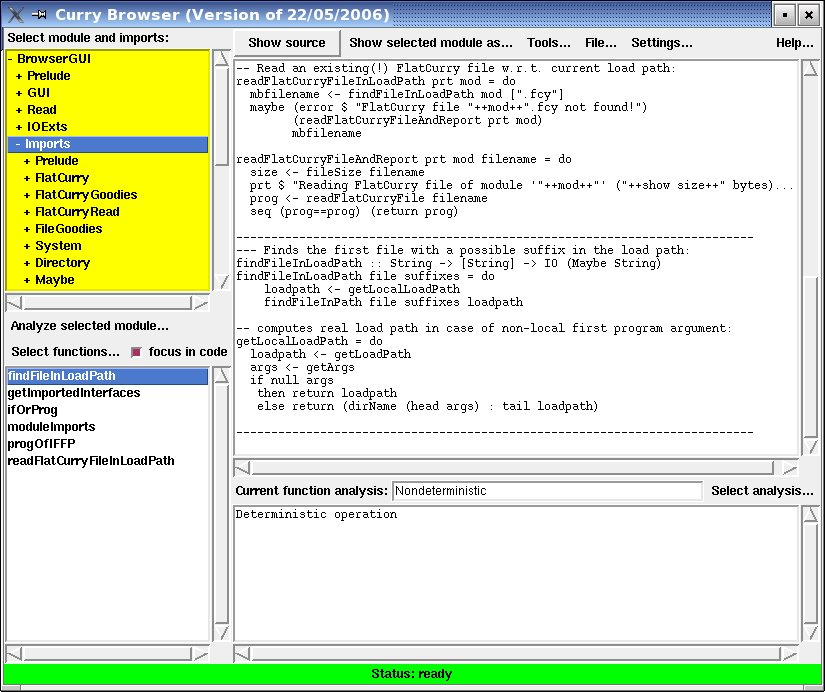
\includegraphics[scale=0.7]{currybrowser.jpg}
\end{center}
\caption{Snapshot of the main window of CurryBrowser\label{fig-currybrowser}}
\end{figure}
%
To get an impression of the use of \cb, Figure~\ref{fig-currybrowser}
shows a snapshot of its use on a particular application
(here: the implementation of \cb).
The upper list box in the left column shows the modules and their imports
in order to browse through the modules of an application.
Similarly to directory browsers, the list of imported modules of a module
can be opened or closed by clicking.
After selecting a module in the list of modules, its source code,
interface, or various other formats of the module can be shown
in the main (right) text area. For instance, one can show
pretty-printed versions of the intermediate flat programs (see below)
in order to see how local function definitions are translated by lambda lifting
\cite{Johnsson85}
or pattern matching is translated into case expressions \cite{Hanus97POPL,Wadler87}.
Since Curry is a language with parametric polymorphism and type inference,
programmers often omit the type signatures when defining functions.
Therefore, one can also view (and store) the selected module as source code where
missing type signatures are added.

Below the list box for selecting modules, there is a menu
(``Analyze selected module'') to analyze all functions
of the currently selected module at once. This is useful
to spot some functions of a module that could be problematic
in some application contexts, like functions that are impure (i.e., the result
depends on the evaluation time) or partially defined (i.e.,
not evaluable on all ground terms).
If such an analysis is selected,
the names of all functions are shown in the
lower list box of the left column (the ``function list'')
with prefixes indicating the properties of the individual functions.

The function list box can be also filled with functions
via the menu ``Select functions''. For instance, all functions
or only the exported functions defined in the currently selected
module can be shown there, or all functions from different modules
that are directly or indirectly called from
a currently selected function.
This list box is central to focus on a function in the
source code of some module or to analyze some function,
i.e., showing their properties. In order to focus on a function,
it is sufficient to check the ``focus on code'' button.
To analyze an individually selected function, one can
select an analysis from the list of available program analyses
(through the menu ``Select analysis'').
In this case, the analysis results are either shown
in the text box below the main text area
or visualized by separate tools, e.g., by a graph drawing tool for
visualizing call graphs.
Some analyses are local, i.e., they need only to consider the local definition
of this function (e.g., ``Calls directly,'' ``Overlapping rules,''
``Pattern completeness''),
where other analyses are global, i.e.,
they consider the definitions of all functions directly or indirectly called
by this function (e.g., ``Depends on,'' ``Solution complete,''
``Set-valued'').
%
Finally, there are a few additional tools integrated into \cb,
for instance, to visualize the import relation between all modules
as a dependency graph. These tools are available through the ``Tools'' menu.

More details about the use of \cb and all built-in analyses
are available through the ``Help'' menu of \cb.


\newpage

\section{CurryTest: A Tool for Testing Curry Programs}
\label{sec-currytest}

CurryTest\index{CurryTest}\index{testing programs}\index{program!testing}
is a simple tool in the PAKCS distribution to write
and run repeatable tests. CurryTest simplifies the task
of writing test cases for a module and executing them.
The tool is easy to use. Assume one has implemented a module \code{MyMod}
and wants to write some test cases to test its functionality,
making regression tests in future versions, etc.
For this purpose, there is a system library \code{Assertion}
(Section~\ref{Library:Assertion}) which
contains the necessary definitions for writing tests.
In particular, it exports an abstract polymorphic type \ccode{Assertion a}
together with the following operations:
\startprog
assertTrue      :: String -> Bool -> Assertion ()
assertEqual     :: String -> a -> a -> Assertion a
assertValues    :: String -> a -> [a] -> Assertion a
assertSolutions :: String -> (a->Success) -> [a] -> Assertion a
assertIO        :: String -> IO a -> a -> Assertion a
assertEqualIO   :: String -> IO a -> IO a -> Assertion a
\stopprog
The expression \ccode{assertTrue $s$ $b$}
is an assertion (named $s$) that the expression $b$ has the value \code{True}.
Similarly, the expression \ccode{assertEqual $s$ $e_1$ $e_2$}
asserts that the expressions $e_1$ and $e_2$
must be equal (i.e., \code{$e_1$==$e_2$} must hold),
the expression \ccode{assertValues $s$ $e$ $vs$} asserts
that $vs$ is the multiset of all values of $e$,
and the expression \ccode{assertSolutions $s$ $c$ $vs$} asserts
that the constraint abstraction $c$ has the multiset of solutions $vs$.
Furthermore, the expression \ccode{assertIO $s$ $a$ $v$}
asserts that the I/O action $a$ yields the value $v$ whenever it is
executed, and
the expression \ccode{assertEqualIO $s$ $a_1$ $a_2$}
asserts that the I/O actions $a_1$ and $a_2$ yields equal values.
The name $s$ provided as a first argument in each assertion
is used in the protocol produced by the test tool.

One can define a test program by importing the module
to be tested together with the module \code{Assertion} and defining
top-level functions of type \code{Assertion} in this module
(which must also be exported).
As an example, consider the following program
that can be used to test some list processing functions:
\startprog
\medskip
import List
import Assertion
\medskip
test1 = assertEqual     "++"     ([1,2]++[3,4]) [1,2,3,4]
\medskip
test2 = assertTrue      "all"    (all (<5) [1,2,3,4])
\medskip
test3 = assertSolutions "prefix" (\labs{}x -> let y free in  x\,++\,y =:= [1,2])
                                 [[],[1],[1,2]]
\medskip
\stopprog
For instance, \code{test1} asserts that the result of evaluating the
expression \code{([1,2]++[3,4])} is equal to \code{[1,2,3,4]}.

We can execute a test suite by the command\pindex{currytest}
\startprog
currytest testList
\stopprog
(\code{currytest} is a program stored in \code{$pakcshome$/bin}
where $pakcshome$ is the installation directory of PAKCS;
see Section~\ref{sec-general}).
In our example, \ccode{testList.curry} is the program containing the
definition of all assertions. This has the effect
that all exported top-level functions
of type \code{Assertion} are tested (i.e., the corresponding
assertions are checked) and the results
(\ccode{OK} or failure) are reported together with the name of each assertion.
%If failures occur, the complete test results are also
%written into a file named \ccode{testList.testlog}.''
For our example above, we obtain the following successful protocol:
\startprog
============================================================
Testing module "testList"...
OK: ++
OK: all
OK: prefix
All tests successfully passed.
============================================================
\stopprog
There is also a graphical interface that summarizes the results
more nicely.\footnote{Due to a bug in older versions of SICStus-Prolog,
it works only with SICStus-Prolog version 3.8.5 (or newer).}
In order to start this interface, one has to add the parameter
\ccode{--window} (or \ccode{-w}), e.g., executing a test suite by
\startprog
currytest --window testList
\stopprog
or
\startprog
currytest -w testList
\stopprog
A snapshot of the interface is shown in Figure~\ref{fig-currytest}.

\begin{figure}%[t]
\begin{center}
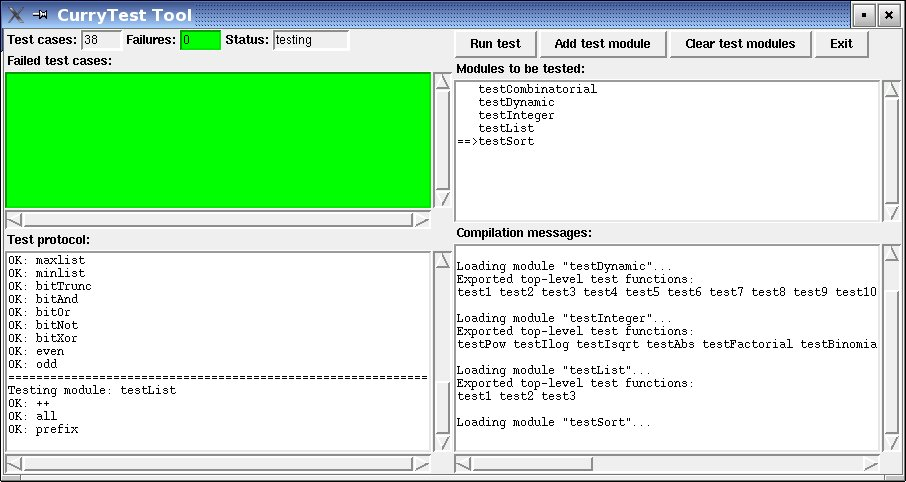
\includegraphics[scale=0.7]{currytest.jpg}
\end{center}
\caption{Snapshot of CurryTest's graphical interface\label{fig-currytest}}
\end{figure}


\newpage

\section{ERD2Curry: A Tool to Generate Programs from ER Specifications}
\label{sec-erd2curry}

ERD2Curry\index{ERD2Curry}\index{database programming}
is a tool to generate Curry code to access and manipulate data
persistently stored from
entity relationship diagrams.\index{entity relationship diagrams}
The idea of this tool is described in detail in
\cite{BrasselHanusMueller08PADL}.
Thus, we describe only the basic steps to use this tool
in the following.

If one creates an entity relationship diagram (ERD)
with the Umbrello UML Modeller, one has to store its
XML description in XMI format (as offered by Umbrello)
in a file, e.g., \ccode{myerd.xmi}.
This description can be compiled into a Curry program by the
command\pindex{erd2curry}
\startprog
erd2curry myerd.xmi
\stopprog
(\code{erd2curry} is a program stored in \code{$pakcshome$/bin}
where $pakcshome$ is the installation directory of PAKCS;
see Section~\ref{sec-general}).
If \code{MyData} is the name of the ERD, the Curry program file
\ccode{MyData.curry} is generated containing all the necessary
database access code as described in \cite{BrasselHanusMueller08PADL}.

If one does not want to use the Umbrello UML Modeller,
one can also create a textual description of the ERD
as a Curry term of type \code{ERD}
(w.r.t.\ the type definition given in module
\code{$pakcshome$/tools/erd2curry/ERD.curry})
and store it in some file, e.g., \ccode{myerd.term}.
This description can be compiled into a Curry program by the
command\pindex{erd2curry}
\startprog
erd2curry -t myerd.term
\stopprog
%
There is also the possibility to visualize an ERD term
as a graph with the graph visualization program \code{dotty}
(for this purpose, it might be necessary to adapt the definition
of the operation \code{dotCmd} in
\code{$pakcshome$/tools/erd2curry/ERD2Graph.curry}
according to your local environment).
This can be done by the command
\startprog
erd2curry -v myerd.term
\stopprog

\paragraph{Inclusion in the Curry application:}
To compile the generated database code, either
include the directory \code{$pakcshome$/tools/erd2curry}
into your Curry load path
(e.g., by setting  the environment variable
\ccode{CURRYPATH}\pindex{CURRYPATH}, see also Section~\ref{sec-modules})
or copy the file
\code{$pakcshome$/tools/erd2curry/ERDGeneric.curry}
into the directory of the generated database code.


\newpage

\section{UI: Declarative Programming of User Interfaces}
\label{sec-ui}

The PAKCS distribution contains a collection of libraries
to implement graphical user interfaces\index{user interface}
as well as web-based user interfaces
from declarative descriptions.
Exploiting these libraries, it is possible
to define the structure and functionality of a user interface
independent from the concrete technology.
Thus, a graphical user interface or a web-based user interface
can be generated from the same description by simply changing
the imported libraries.
This programming technique is described in detail in
\cite{HanusKluss09PADL}.

The libraries implementing these user interfaces are contained
in the directory
\startprog
$pakcshome$/tools/ui
\stopprog
Thus, in order to compile programs containing such user interface
specifications, one has to
include the directory \code{$pakcshome$/tools/ui}
into the Curry load path
(e.g., by setting  the environment variable
\ccode{CURRYPATH}\pindex{CURRYPATH}, see also Section~\ref{sec-modules}).
The directory
\startprog
$pakcshome$/tools/ui/examples
\stopprog
contains a few examples for such user interface specifications.


\newpage

\section{Preprocessing FlatCurry Files}
\label{sec-pakcspp}

The current parser allows to apply transformations on the intermediate
FlatCurry files after they are generated from the
corresponding Curry source file.
Currently, only the FlatCurry file corresponding to the main module
can be transformed.

A transformation can be specified as follows:
\begin{enumerate}
\item {\bf Options to \code{pakcs/bin/parsecurry}:}
\begin{description}
\item[\fbox{\code{--fpopt}}]\pindex{-fpopt}
Apply functional pattern optimization
(see \code{pakcs/tools/optimize/NonStrictOpt.curry} for details).

\item[\fbox{\code{--compact}}]\pindex{--compact}
Apply code compactification after parsing, i.e., transform the main
module and all its imported into one module and delete all
non-accessible functions.

\item[\fbox{\code{--compactexport}}]
Similar to \code{--compact} but delete all functions that are not accessible
from the exported functions of the main module.

\item[\fbox{\code{--compactmain:f}}]
Similar to \code{--compact} but delete all functions that are not accessible
from the function \ccode{f} of the main module.

\item[\fbox{\code{--fcypp cmd}}]\pindex{--fcypp}
Apply command \code{cmd} to the main module after parsing. This is useful to
integrate your own transformation into the compilation process.
Note that the command \ccode{cmd prog} should perform a transformation
on the FlatCurry file \code{prog.fcy}, i.e., it replaces the FlatCurry
file by a new one.
\end{description}

\item {\bf Setting the environment variable \code{FCYPP}:}\pindex{FCYPP}\\
For instance, setting \code{FCYPP} by
\startprog
export FCYPP="--fpopt"
\stopprog
will apply the functional pattern optimization if programs are compiled
and loaded in the PAKCS programming environment.


\item {\bf Putting options into the source code:}\pindex{PAKCS_OPTION_FCYPP}\\
If the source code contains a line with a comment of the form (the comment
must start at the beginning of the line)
\startprog
\{-\# PAKCS_OPTION_FCYPP <options> \#-\}
\stopprog
then the transformations specified by \code{<options>} are applied after
translating the source code into FlatCurry code. For instance,
the functional pattern optimization can be set by the comment
\startprog
\{-\# PAKCS_OPTION_FCYPP --fpopt \#-\}
\stopprog
in the source code. Note that this comment must be in a single line 
of the source program. If there are multiple lines containing such comments,
only the first one will be considered.
\end{enumerate}
\paragraph{Multiple options:}
Note that an arbitrary number of transformations can be specified
by the methods described above.
If several specifications for preprocessing FlatCurry files are used,
they are executed in the following order:
\begin{enumerate}
\item all transformations specified by the environemnt variable
\code{FCYPP} (from left to right)
\item all transformations specified as command line options of parsecurry
   (from left to right)
\item all transformations specified by a comment line in the source code
   (from left to right)
\end{enumerate}


\newpage

\section{Technical Problems}

Due to the fact that Curry is intended to implement
distributed systems (see Appendix~\ref{sec-ports}),
it might be possible that some technical problems
arise due to the use of sockets for implementing these
features. Therefore, this section gives some information
about the technical requirements of PAKCS and how to solve
problems due to these requirements.

There is one fixed port that is used by the implementation of PAKCS:
\begin{description}
\item[Port 8766:] This port is used by the
{\bf Curry Port Name Server} (CPNS) to implement symbolic names for
ports in Curry (see Appendix~\ref{sec-ports}).
If some other process uses this port on the machine,
the distribution facilities defined in the module \code{Ports}
(see Appendix~\ref{sec-ports}) cannot be used.
\end{description}
If these features do not work, you can try to find out
whether this port is in use by the shell command
\ccode{netstat -a | fgrep 8766} (or similar).

The CPNS is implemented as a demon listening on its port 8766
in order to serve requests about registering a new symbolic
name for a Curry port or asking the physical port number
of a Curry port. The demon will be automatically started for
the first time on a machine when a user compiles a program
using Curry ports. It can also be manually started and terminated by the
scripts \code{$pakcshome$/cpns/start} and
\code{$pakcshome$/cpns/stop}.
If the demon is already running, the command \code{$pakcshome$/cpns/start}
does nothing (so it can be always executed
before invoking a Curry program using ports).

If you detect any further technical problem,
please write to
\begin{center}
\code{mh@informatik.uni-kiel.de}
\end{center}

\newpage

\addcontentsline{toc}{section}{Bibliography}
\bibliography{manual}
\bibliographystyle{plain}

\newpage
\appendix

\section{Libraries of the PAKCS Distribution}
\label{sec:libraries}

{\setlength{\parindent}{0.0cm}

The PAKCS compiler system provides an extensive collection
of libraries for application programming.
The libraries for arithmetic constraints over real numbers,
finite domain constraints,
ports for concurrent and distributed programming, and
meta-programming by representing Curry programs in Curry
are described in the following subsection in more detail.
The complete set of libraries with all exported types and functions
are described in the further subsections.
For a more detailed online documentation of all libraries of PAKCS,
see \url{http://www.informatik.uni-kiel.de/~pakcs/lib/index.html}.

\subsection{Constraints, Ports, Meta-Programming}

\subsubsection{Arithmetic Constraints}

The primitive entities for the use of arithmetic constraints
are defined in the system module \code{CLPR}
(cf.\ Section~\ref{sec-modules}), i.e., in order to use them,
the program must contain the import declaration
\startprog
import CLPR
\stopprog
Floating point arithmetic is supported in PAKCS
via arithmetic constraints, i.e., the equational constraint
\ccode{2.3 +.~x =:= 5.5} is solved by binding \code{x} to \code{3.2}
(rather than suspending the evaluation of the addition,
as in corresponding constraints on integers like
\ccode{3+x=:=5}). All operations related to
floating point numbers are suffixed by \ccode{.}.
The following functions and constraints on floating point
numbers are supported in PAKCS:
\begin{description}
\item[\code{(+.)   :: Float -> Float -> Float}]~\\
Addition on floating point numbers.
\item[\code{(-.)   :: Float -> Float -> Float}]~\\
Subtraction on floating point numbers.
\item[\code{(*.)   :: Float -> Float -> Float}]~\\
Multiplication on floating point numbers.
\item[\code{(/.)   :: Float -> Float -> Float}]~\\
Division on floating point numbers.
\item[\code{(<.)   :: Float -> Float -> Success}]~\\
Comparing two floating point numbers with the ``less than'' relation.
\item[\code{(>.)   :: Float -> Float -> Success}]~\\
Comparing two floating point numbers with the ``greater than'' relation.
\item[\code{(<=.)  :: Float -> Float -> Success}]~\\
Comparing two floating point numbers with the ``less than or equal'' relation.
\item[\code{(>=.)  :: Float -> Float -> Success}]~\\
Comparing two floating point numbers with the ``greater than or equal''
relation.
\item[\code{i2f    :: Int -> Float}]~\\
Converting an integer number into a floating point number.
\end{description}
As an example, consider a constraint \code{mortgage}
which relates the principal \code{p},
the lifetime of the mortgage in months \code{t},
the monthly interest rate \code{ir},
the monthly repayment \code{r},
and the outstanding balance at the end of the lifetime \code{b}.
The financial calculations
can be defined by the following two rules in Curry (the second rule
describes the repeated accumulation of the interest):
\startprog
~
import CLPR
~
mortgage p t ir r b | t >. 0.0 \& t <=. 1.0  --lifetime not more than 1 month?
                    =  b =:= p *. (1.0 +. t *. ir) -. t*.r \vspace{1ex}
mortgage p t ir r b | t >. 1.0               --lifetime more than 1 month?
                    =  mortgage (p *. (1.0+.ir)-.r) (t-.1.0) ir r b
~
\stopprog
Then we can calculate the monthly payment for paying back
a loan of \$100,000 in 15 years with a monthly interest rate of 1\%
by solving the goal
\startprog
mortgage 100000.0 180.0 0.01 r 0.0
\stopprog
which yields the solution \code{r=1200.17}.

Note that only linear arithmetic equalities or inequalities
are solved by the constraint solver. Non-linear constraints
like \ccode{x *.~x =:= 4.0} are suspended until they become
linear.


\subsubsection{Finite Domain Constraints}

Finite domain constraints are constraints where all variables
can only take a finite number of possible values.
For simplicity, the domain of finite domain variables are
identified with a subset of the integers, i.e., the type
of a finite domain variable is \code{Int}. The arithmetic
operations related to finite domain variables are suffixed by \ccode{\#}.
The following functions and constraints for finite domain constraint solving
are currently supported in PAKCS:\footnote{Note that
this library is based on the corresponding library of SICStus-Prolog
but does not implement the complete functionality of the SICStus-Prolog library.
However, using the PAKCS interface for external functions (see
Appendix~\ref{sec-external-functions}), it is relatively
easy to provide the complete functionality.}

\begin{description}
\item[\code{domain :: [Int] -> Int -> Int -> Success}]~\\
The constraint \ccode{domain [$x_1,\ldots,x_n$] $l$ $u$}
is satisfied if the domain of all variables $x_i$ is the interval $[l,u]$.
\item[\code{(+\#)   :: Int -> Int -> Int}]~\\
Addition on finite domain values.
\item[\code{(-\#)   :: Int -> Int -> Int}]~\\
Subtraction on finite domain values.
\item[\code{(*\#)   :: Int -> Int -> Int}]~\\
Multiplication on finite domain values.
\item[\code{(=\#)   :: Int -> Int -> Success}]~\\
Equality of finite domain values.
\item[\code{(/=\#)  :: Int -> Int -> Success}]~\\
Disequality of finite domain values.
\item[\code{(<\#)   :: Int -> Int -> Success}]~\\
``less than'' relation on finite domain values.
\item[\code{(<=\#)  :: Int -> Int -> Success}]~\\
``less than or equal'' relation on finite domain values.
\item[\code{(>\#)   :: Int -> Int -> Success}]~\\
``greater than'' relation on finite domain values.
\item[\code{(>=\#)  :: Int -> Int -> Success}]~\\
``greater than or equal'' relation on finite domain values.
\item[\code{sum :: [Int] -> (Int -> Int -> Success) -> Int -> Success}]~\\
The constraint \ccode{sum [$x_1,\ldots,x_n$] $op$ $x$}
is satisfied if all $x_1+\cdots + x_n \mathrel{op} x$ is satisfied,
where $op$ is one of the above finite domain constraint relations
(e.g., \ccode{=\#}).
\item[\code{scalar_product :: [Int] -> [Int] -> (Int -> Int -> Success) -> Int -> Success}]~\\
The constraint \ccode{scalar_product [$c_1,\ldots,c_n$] [$x_1,\ldots,x_n$] $op$ $x$}
is satisfied if all $c_1 x_1+\cdots + c_n x_n \mathrel{op} x$ is satisfied,
where $op$ is one of the above finite domain constraint relations.
\item[\code{count :: Int -> [Int] -> (Int -> Int -> Success) -> Int -> Success}]~\\
The constraint \ccode{count $k$ [$x_1,\ldots,x_n$] $op$ $x$}
is satisfied if all $k \mathrel{op} x$ is satisfied,
where $n$ is the number of the $x_i$ that are equal to $k$ and
$op$ is one of the above finite domain constraint relations.
\item[\code{all_different :: [Int] -> Success}]~\\
The constraint \ccode{all_different [$x_1,\ldots,x_n$]}
is satisfied if all $x_i$ have pairwise different values.
\item[\code{labeling :: [LabelingOption] -> [Int] -> Success}]~\\
The constraint \ccode{labeling $os$ [$x_1,\ldots,x_n$]}
non-deterministically instantiates all $x_i$ to the values
of their domain according to the options $os$ (see the module documentation
for further details about these options).
\end{description}
These entities are defined in the system module \code{CLPFD}
(cf.\ Section~\ref{sec-modules}), i.e., in order to use it,
the program must contain the import declaration
\startprog
import CLPFD
\stopprog
As an example, consider the classical \ccode{send+more=money} problem
where each letter must be replaced by a different digit such that this
equation is valid and there are no leading zeros.
The usual way to solve finite domain constraint problems
is to specify the domain of the involved variables followed
by a specification of the constraints and the labeling
of the constraint variables in order to start the search for solutions.
Thus, the \ccode{send+more=money} problem can be solved as follows:
\startprog
~
import CLPFD
~
smm l =
        l =:= [s,e,n,d,m,o,r,y] \&
        domain l 0 9 \&
        s >\# 0 \&
        m >\# 0 \&
        all_different l  \&
                         1000 *\# s +\# 100 *\# e +\# 10 *\# n +\# d
        +\#               1000 *\# m +\# 100 *\# o +\# 10 *\# r +\# e
        =\# 10000 *\# m +\# 1000 *\# o +\# 100 *\# n +\# 10 *\# e +\# y \&
        labeling [FirstFail] l
        where s,e,n,d,m,o,r,y free
~
\stopprog
Then we can solve this problem by evaluating the goal
\ccode{smm [s,e,n,d,m,o,r,y]} which yields the unique solution
\code{\{s=9,e=5,n=6,d=7,m=1,o=0,r=8,y=2\}}.


\subsubsection{Ports: Distributed Programming in Curry}
\label{sec-ports}

To support the development of concurrent and distributed applications,
PAKCS supports internal and external ports\index{ports} as
described in \cite{Hanus99PPDP}.
Since \cite{Hanus99PPDP} contains a detailed description of this
concept together with various programming examples, we only summarize here
the functions and constraints supported for ports in PAKCS.

The basic datatypes, functions, and constraints for ports
are defined in the system module \code{Ports}
(cf.\ Section~\ref{sec-modules}), i.e., in order to use ports,
the program must contain the import declaration
\startprog
import Ports
\stopprog
This declaration includes the following entities in the program:
\begin{description}
\item[\code{Port a}\pindex{Port}]~\\
This is the datatype of a port to which one can send messages of type \code{a}.

\item[\code{openPort :: Port a -> [a] -> Success}]~\\
The constraint \ccode{openPort p s}\pindex{openPort}
establishes a new \emph{internal port}
\code{p} with an associated message stream \code{s}. \code{p} and \code{s} must be
unbound variables,
otherwise the constraint fails (and causes a runtime error).

\item[\code{send :: a -> Port a -> Success}]~\\
The constraint \ccode{send m p}\pindex{send}
is satisfied if \code{p} is constrained
to contain the message \code{m}, i.e., \code{m} will be sent to the port
\code{p} so that it appears in the corresponding stream.

\item[\code{doSend :: a -> Port a -> IO ()}]~\\
The I/O action \ccode{doSend m p}\pindex{doSend} solves the constraint
\ccode{send m p} and returns nothing.

\item[\code{openNamedPort :: String -> IO [a]}]~\\
The I/O action \ccode{openNamedPort n}\pindex{openNamedPort}
opens a new \emph{external port} with
symbolic name \code{n} and returns the associated stream of messages.

\item[\code{connectPort :: String -> IO (Port a)}]~\\
The I/O action \ccode{connectPort n}\pindex{connectPort}
returns a port with symbolic name
\code{n} (i.e., \code{n} must have the form ``\emph{portname@machine})
to which one can send messages by the \code{send} constraint.
Currently, no dynamic type checking is done for external ports,
i.e., sending messages of the wrong type to a port might lead to
a failure of the receiver.
\end{description}

\paragraph{Restrictions:}
Every expression, possibly containing logical variables, can be sent to
a port. However, as discussed in \cite{Hanus99PPDP},
port communication is strict, i.e., the expression is
evaluated to normal form before sending it by the
constraint \code{send}. Furthermore, if messages containing
logical variables are sent to \emph{external ports},
the behavior is as follows:
\begin{enumerate}
\item The sender waits until all logical variables in the message
have been bound by the receiver.
\item The binding of a logical variable received by a process
is sent back to the sender of this logical variable only if
it is bound to a \emph{ground} term, i.e., as long as the binding contains
logical variables, the sender is not informed about the binding
and, therefore, the sender waits.
\end{enumerate}

\paragraph{External ports on local machines:}
The implementation of external ports assumes that the
host machine running the application is connected to the Internet
(i.e., it uses the standard IP address of the host machine
for message sending). If this is not the case and the application
should be tested by using external ports only on the local host
without a connection to the Internet,
the environment variable \ccode{PAKCS_LOCALHOST}\pindex{PAKCS_LOCALHOST}
must be set to \ccode{yes}
\emph{before PAKCS system is started}.
In this case, the IP address \code{127.0.0.1} and the hostname
\ccode{localhost} are used for identifying the local machine.

\paragraph{Selection of Unix sockets for external ports:}
The implementation of ports uses sockets to communicate
messages sent to external ports.
Thus, if a Curry program uses the
I/O action \code{openNamedPort}\pindex{openNamedPort}
to establish an externally visible server,
PAKCS selects a Unix socket for the port communication.
Usually, a free socket is selected by the operating system.
If the socket number should be fixed in an application (e.g.,
because of the use of firewalls\index{firewall} that allow only
communication over particular sockets), then one
can set the environment variable \ccode{PAKCS_SOCKET}\pindex{PAKCS_SOCKET}
to a distinguished socket number before the PAKCS system is started.
This has the effect that PAKCS uses only this socket
number for communication (even for several external ports
used in the same application program).

\paragraph{Debugging:}
To debug distributed systems,
it is sometimes helpful to see all messages sent to external ports.
This is supported by the environment variable
\ccode{PAKCS_TRACEPORTS}.\pindex{PAKCS_TRACEPORTS}
If this variable is set to \ccode{yes}
\emph{before the PAKCS system is started}, then all
connections to external ports and all
messages sent and received on external ports are
printed on the standard error stream.


\subsubsection{AbstractCurry and FlatCurry: Meta-Programming in Curry}
\label{sec-flatcurry}

\index{AbstractCurry}
\index{FlatCurry}
To support meta-programming, i.e., the manipulation of Curry programs
in Curry, there are system modules \code{FlatCurry} and \code{AbstractCurry}
(stored in the directory \ccode{$pakcshome$/lib/meta})
which define datatypes for the representation
of Curry programs.
\code{AbstractCurry} is a more direct representation of a Curry program,
whereas \code{FlatCurry} is a simplified representation
where local function definitions are replaced by global definitions
(i.e., lambda lifting has been performed) and pattern matching
is translated into explicit case/or expressions.
Thus, \code{FlatCurry} can be used for more back-end oriented
program manipulations (or, for writing new back ends for Curry),
whereas \code{AbstractCurry} is intended for manipulations of
programs that are more oriented towards the source program.

Both modules contain predefined I/O actions to read programs
in the \code{AbstractCurry} (\code{readCurry}\pindex{readCurry})
or \code{FlatCurry}
(\code{readFlatCurry}\pindex{readFlatCurry}) format.
These actions parse the corresponding source program and return
a data term representing this program (according to the definitions
in the modules \code{AbstractCurry} and \code{FlatCurry}).

Since all datatypes are explained in detail in these modules,
we refer to the online documentation\footnote{%
\url{http://www.informatik.uni-kiel.de/~pakcs/lib/CDOC/FlatCurry.html} and
\url{http://www.informatik.uni-kiel.de/~pakcs/lib/CDOC/AbstractCurry.html}}
of these modules.

As an example, consider a program file \ccode{test.curry}
containing the following two lines:
\startprog
rev []     = []
rev (x:xs) = (rev xs) ++ [x]
\stopprog
Then the I/O action \code{(FlatCurry.readFlatCurry "test")} returns the
following term:
\startprog
 (Prog "test"
  ["Prelude"]
  []
  [Func ("test","rev") 1 Public
        (FuncType (TCons ("Prelude","[]") [(TVar 0)])
                  (TCons ("Prelude","[]") [(TVar 0)]))
        (Rule [0]
           (Case Flex (Var 0)
              [Branch (Pattern ("Prelude","[]") [])
                  (Comb ConsCall ("Prelude","[]") []),
               Branch (Pattern ("Prelude",":") [1,2])
                  (Comb FuncCall ("Prelude","++")
                        [Comb FuncCall ("test","rev") [Var 2],
                         Comb ConsCall ("Prelude",":")
                              [Var 1,Comb ConsCall ("Prelude","[]") []]
                        ])
              ]))]
  []
 )
\stopprog


%%%%%%%%%%%%%%%%%%%%%%%%%%%%%%%%%%%%%%%%%%%%%%%%%%%%%%%%%%%%%%%%%%%%%%%%%
% Definitions in order to LaTeX documents generated by "currydoc --tex"
%%%%%%%%%%%%%%%%%%%%%%%%%%%%%%%%%%%%%%%%%%%%%%%%%%%%%%%%%%%%%%%%%%%%%%%%%

\newcommand{\currymodule}[1]{\subsubsection{Library #1}\label{Library:#1}}
\newcommand{\currytypesstart}{\subsubsection*{Exported types:}}
\newcommand{\currytypesstop}{}
\newcommand{\currytypesynstart}[2]{{\tt type #2}\pindex{#1} \begin{quote}}
\newcommand{\currytypesynstop}{\end{quote}}
\newcommand{\currydatastart}[1]{{\tt data #1}\pindex{#1} \begin{quote}}
\newcommand{\currydatacons}{\end{quote}%
\begin{itemize}\item[] \hspace{-4ex}\emph{Exported constructors:}}
\newcommand{\currydatastop}{\end{itemize}}
\newcommand{\curryconsstart}[2]{\item {\tt #1~::~#2}\par}
\newcommand{\curryfuncstart}{\subsubsection*{Exported functions:}}
\newcommand{\curryfuncstop}{}
\newcommand{\curryfunctionstart}[2]{#2\pindex{#1}\begin{quote}}
\newcommand{\curryfunctionstop}{\end{quote}}
\newcommand{\curryfuncsig}[2]{{\tt #1~::~#2}}


\subsection{General Libraries}

\input{lib/AllSolutions}
\input{lib/Assertion}
\input{lib/Char}
\input{lib/CLPFD}
\input{lib/CLPR}
\input{lib/CLPB}
\input{lib/Combinatorial}
\input{lib/Constraint}
\input{lib/CSV}
\input{lib/Database}
\input{lib/DaVinci}
\input{lib/Directory}
\input{lib/Dynamic}
\input{lib/FileGoodies}
\input{lib/Float}
\input{lib/Global}
\input{lib/GlobalVariable}
\input{lib/GUI}
\input{lib/Integer}
\input{lib/IO}
\input{lib/IOExts}
\input{lib/JavaScript}
\input{lib/KeyDatabase}
\input{lib/KeyDatabaseSQLite}
\input{lib/KeyDB}
\input{lib/List}
\input{lib/Maybe}
\input{lib/NamedSocket}
\input{lib/Parser}
\input{lib/Ports}
\input{lib/Pretty}
\input{lib/Profile}
\input{lib/PropertyFile}
\input{lib/Read}
\input{lib/ReadNumeric}
\input{lib/ReadShowTerm}
\input{lib/SetFunctions}
\input{lib/Socket}
\input{lib/System}
\input{lib/Time}
%\input{lib/Tk}
\input{lib/Unsafe}


\subsection{Data Structures and Algorithms}

\input{lib/Array}
\input{lib/Dequeue}
\input{lib/FiniteMap}
\input{lib/GraphInductive}
\input{lib/Random}
\input{lib/RedBlackTree}
\input{lib/SetRBT}
\input{lib/Sort}
\input{lib/TableRBT}
\input{lib/Traversal}

\subsection{Libraries for Web Applications}

\input{lib/CategorizedHtmlList}
\input{lib/HTML}
\input{lib/HtmlParser}
\input{lib/Mail}
\input{lib/Markdown}
\input{lib/WUI}
\input{lib/URL}
\input{lib/XML}
\input{lib/XmlConv}

\subsection{Libraries for Meta-Programming}

\input{lib/AbstractCurry}
\input{lib/AbstractCurryPrinter}
\input{lib/CompactFlatCurry}
\input{lib/CurryStringClassifier}
\input{lib/FlatCurry}
\input{lib/FlatCurryGoodies}
\input{lib/FlatCurryRead}
\input{lib/FlatCurryShow}
\input{lib/FlatCurryTools}
\input{lib/FlatCurryXML}
\input{lib/FlexRigid}
\input{lib/PrettyAbstract}

} % end setlength parindent

\newpage

\input{markdown_syntax}

\newpage

\begin{figure}%[t]
\begin{center}
 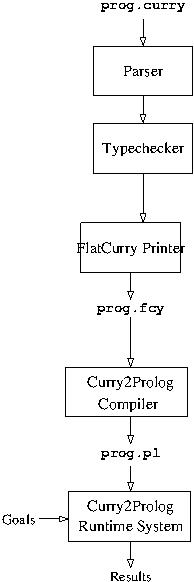
\includegraphics[scale=0.85]{pakcs_overview.jpg}
\end{center}\vspace{-5ex}
\caption{Overview of PAKCS\label{fig-pakcs}}
\end{figure}

\section{Overview of the PAKCS Distribution}

A schematic overview of the various components contained in
the distribution of PAKCS and the
translation process of programs inside PAKCS is shown in
Figure~\ref{fig-pakcs} on page~\pageref{fig-pakcs}.
In this figure, boxes denote different components of PAKCS
and names in boldface denote files containing
various intermediate representations during the translation
process (see Section~\ref{sec-auxfiles} below).
The PAKCS distribution contains a front end for reading (parsing and
type checking) Curry programs that can be also used by
other Curry implementations.
The back end (formerly known as ``Curry2Prolog''\index{Curry2Prolog})
compiles Curry programs into Prolog programs.
It also support constraint solvers for
arithmetic constraints over real numbers and finite domain constraints,
and further libraries for GUI programming, meta-programming etc.
Currently, it does not implement encapsulated search in full generality
(only a strict version of \code{findall} is supported),
and concurrent threads are not executed in a fair manner.


\newpage

\section{Auxiliary Files}
\label{sec-auxfiles}

During the translation and execution of a Curry program with PAKCS,
various intermediate representations of the source program are created
and stored in different files which are shortly explained in this section.
If you use the PAKCS, it is not necessary to know about
these auxiliary files because they are automatically generated
and updated. You should only remember the command for deleting
all auxiliary files (\ccode{cleancurry}, see Section~\ref{sec-general})
to clean up your directories.

The various components of PAKCS create
the following auxiliary files.
\begin{description}
\item[\code{prog.fcy}:] This file contains the Curry program
in the so-called ``FlatCurry'' representation where all functions are global
(i.e., lambda lifting has been performed) and pattern matching
is translated into explicit case/or expressions
(compare Appendix~\ref{sec-flatcurry}).
This representation might be useful for other back ends and
compilers for Curry and is the basis doing meta-programming in Curry.
This file is implicitly
generated when a program is read by PAKCS.
It can be also explicitly generated by the command\pindex{parsecurry}
\startprog
parsecurry --flat prog
\stopprog
The FlatCurry representation of a Curry program is usually
generated by the front-end after parsing, type checking and eliminating
local declarations.
If $dir$ is the directory where the Curry program is stored,
the corresponding FlatCurry program is stored in the directory
\ccode{$dir$/.curry}.

\item[\code{prog.fint}:] This file contains the interface
of the program in the so-called ``FlatCurry'' representation,
i.e., it is similar to \code{prog.fcy} but contains only exported
entities and the bodies of all functions omitted (i.e., ``external'').
This representation is useful for providing a fast access
to module interfaces.
This file is implicitly generated by the command\pindex{parsecurry}
\startprog
parsecurry --flat prog
\stopprog
and stored in the same directory as \code{prog.fcy}.

\item[\code{prog.pl}:] This file contains a Prolog program
as the result of translating the Curry program with PAKCS.
If $dir$ is the directory where the Curry program is stored,
the corresponding Prolog program is stored in the directory
\ccode{$dir$/.curry/.pakcs}.

\item[\code{prog.po}:] This file contains the Prolog program
\code{prog.pl} in an intermediate format for faster loading.
This file is stored in the same directory as \code{prog.pl}.

\item[\code{prog.state}:] This file contains the saved state
after compiling and saving a program with PAKCS
(see Section~\ref{sec-use-curry2prolog}).

\end{description}


\newpage


\section{Changing the Prelude or System Modules}

The standard prelude, which is automatically imported into each Curry program,
and all system modules containing datatypes and functions
useful for application programming
(cf.\ Appendix~\ref{sec:libraries})
are stored in the system module directory \ccode{$pakcshome$/lib}
(and its subdirectories).
If you change any of these modules,
you have to recompile the complete system by
executing \code{make} in the directory $pakcshome$.



\newpage

\section{External Functions}
\label{sec-external-functions}

\index{function!external}\index{external function}
Currently, PAKCS has no general interface to external functions.
Therefore, if a new external function should be added
to the system, this function must be declared as \code{external}
in the Curry source code
and then an implementation for this external function
must be inserted in the corresponding back end.
An external function is defined as follows in the Curry source code:
\begin{enumerate}
\item
Add a type declaration for the external function somewhere
in the body of the appropriate file (usually, the prelude
or some system module).
\item
For external functions it is not allowed to define any
rule since their semantics is determined by an external implementation.
Instead of the defining rules, you have to write
\startprog
f external
\stopprog
somewhere in the file containing the type declaration for 
the external function \code{f}.
\end{enumerate}
For instance, the addition on integers can be declared as
an external function as follows:
\startprog
(+) :: Int -> Int -> Int
(+) external
\stopprog
The further modifications to be done for an inclusion of
an external function has to be done in the back end.
A new external function is added to the back end of PAKCS
by informing the compiler about the existence of an external function
and adding an implementation of this function in the run-time
system. Therefore, the following items must be added
in the PAKCS compiler system:
\begin{enumerate}
\item
If the Curry module \code{Mod} contains external functions,
there must be a file named \code{Mod.prim_c2p} containing the
specification of these external functions. The contents of this file
is in XML format and has the following general structure:\footnote{%
\url{http://www.informatik.uni-kiel.de/~pakcs/primitives.dtd} contains a DTD
describing the exact structure of these files.}
\startprog
<primitives>
  \emph{specification of external function $f_1$}
  \ldots
  \emph{specification of external function $f_n$}
</primitives>
\stopprog
The specification of an external function $f$
with arity $n$ has the form
\startprog
<primitive name="$f$" arity="$n$">
  <library>lib</library>
  <entry>pred</entry>
</primitive>
\stopprog
where \code{lib} is the Prolog library (stored in the directory of the
Curry module or in the global directory
\code{$pakcshome$/curry2prolog/lib_src}) containing the code implementing this
function and \code{pred} is a predicate name in this library
implementing this function. Note that the function $f$ must be
declared in module \code{Mod}: either as an external function
or defined in Curry by equations. In the latter case,
the Curry definition is not translated but calls to this function
are redirected to the Prolog code specified above.

Furthermore, the list of specifications can also contain entries of the form
\startprog
<ignore name="$f$" arity="$n$" />
\stopprog
for functions $f$ with arity $n$ that are declared in module \code{Mod}
but should be ignored for code generation, e.g., since they are
never called w.r.t.\ to the current implementation of external functions.
For instance, this is useful when functions that can
be defined in Curry should be (usually more efficiently) are implemented
as external functions.

Note that the arguments are passed in their current (possibly unevaluated) form.
Thus, if the external function requires the arguments to be evaluated
in a particular form, this must be done before calling the external function.
For instance, the external function for adding two integers
requires that both arguments must be evaluated to non-variable head normal form
(which is identical to the ground constructor normal form). Therefore,
the function \ccode{+} is specified in the prelude by
\startprog
(+)   :: Int -> Int -> Int
x + y = (prim_Int_plus \$\# y) \$\# x
\medskip
prim_Int_plus :: Int -> Int -> Int
prim_Int_plus external
\stopprog
where \code{prim_Int_plus} is the actual external function implementing
the addition on integers. Consequently, the specification file
\code{Prelude.prim_c2p} has an entry of the form
\startprog
<primitive name="prim_Int_plus" arity="2">
  <library>prim_standard</library>
  <entry>prim_Int_plus</entry>
</primitive>
\stopprog
where the Prolog library \code{prim_standard.pl} contains the Prolog code
implementing this function.

\item
For most external functions, a \emph{standard interface} is
generated by the compiler so that an $n$-ary function can be
implemented by an $(n+1)$-ary predicate where the last argument must
be instantiated to the result of evaluating the function.  The
standard interface can be used if all arguments are ensured to be
fully evaluated (e.g., see definition of \code{(+)} above) and no
suspension control is necessary, i.e., it is ensured that the
external function call does not suspend for all arguments.
Otherwise, the raw interface (see below) must be used.  For
instance, the Prolog code implementing \code{prim_Int_plus}
contained in the Prolog library \code{prim_standard.pl} is as
follows (note that the arguments of \code{(+)} are passed in reverse
order to \code{prim_Int_plus} in order to ensure a left-to-right
evaluation of the original arguments by the calls to \code{(\$\#)}):
\startprog
prim_Int_plus(Y,X,R) :- R is X+Y.
\stopprog

\item
The \emph{standard interface for I/O actions}, i.e., external functions
with result type \code{IO~a}, assumes that the I/O action
is implemented as a predicate (with a possible side effect)
that instantiates the last argument to the returned value of type \ccode{a}.
For instance, the primitive predicate \code{prim_getChar}
implementing prelude I/O action \code{getChar}
can be implemented by the Prolog code
\startprog
prim_getChar(C) :- get_code(N), char_int(C,N).
\stopprog
where \code{char_int} is a predicate relating the internal
Curry representation of a character with its ASCII value.

\item
If some arguments passed to the external functions are not fully evaluated
or the external function might suspend, the implementation must follow
the structure of the PAKCS run-time system by using
the \emph{raw interface}. In this case, the name of the external entry
must be suffixed by \ccode{[raw]} in the \code{prim_c2p} file.
For instance, if we want to use the raw interface for the external function
\code{prim_Int_plus},
the specification file \code{Prelude.prim_c2p} must have an entry of the form
\startprog
<primitive name="prim_Int_plus" arity="2">
  <library>prim_standard</library>
  <entry>prim_Int_plus[raw]</entry>
</primitive>
\stopprog
In the raw interface, the actual implementation of an $n$-ary external function consists
of the definition of an $(n+3)$-ary predicate $pred$.
The first $n$ arguments are the corresponding actual arguments.
The $(n+1)$-th argument is a free variable which must be
instantiated to the result of the function call after
successful execution. The last two arguments
control the suspension behavior of the function
(see \cite{AntoyHanus00FROCOS} for more details):
The code for the predicate $pred$
should only be executed when the $(n+2)$-th argument
is not free, i.e., this predicate has always the
SICStus-Prolog block declaration
\startprog
?- block $pred$(?,\ldots,?,-,?).
\stopprog
In addition, typical external functions should suspend
until the actual arguments are instantiated. This can be ensured
by a call to \code{ensureNotFree} or \code{(\$\#)}
before calling the external function. Finally, the
last argument (which is a free variable at call time)
must be unified with the $(n+2)$-th argument
after the function call is successfully evaluated
(and does not suspend). Additionally, the actual (evaluated) arguments
must be dereferenced before they are accessed.
Thus, an implementation
of the external function for adding integers is as follows in the raw interface:
\startprog
?- block prim_Int_plus(?,?,?,-,?).
prim_Int_plus(RY,RX,Result,E0,E) :-
     deref(RX,X), deref(RY,Y), Result is X+Y, E0=E.
\stopprog
Here, \code{deref} is a predefined predicate for dereferencing the
actual argument into a constant (and \code{derefAll} for dereferencing
complex structures).
\end{enumerate}
%
The Prolog code implementing the external functions must be accessible to the run-time
system of PAKCS by putting it into the directory containing the corresponding
Curry module or into the system directory
\code{$pakcshome$/curry2prolog/lib_src}.
Then it will be automatically loaded into the run-time environment
of each compiled Curry program.

Note that arbitrary functions implemented in C or Java can be connected to
PAKCS by using the corresponding interfaces of underlying Prolog system.


\newpage
\addcontentsline{toc}{section}{Index}
\printindex


\end{document}

\clearpage
\documentclass[11pt,fleqn]{article}

\usepackage{latexsym}
\usepackage{makeidx}
\usepackage{url}
\usepackage{xspace}
\usepackage{graphicx}

\input{version}

%%% ------------------------------------------------------------------

\usepackage[colorlinks,linkcolor=blue]{hyperref}
\hypersetup{bookmarksopen=true}
\hypersetup{bookmarksopenlevel=0}
\hypersetup{pdftitle={PAKCS: The Portland Aachen Kiel Curry System}}
\hypersetup{pdfauthor={Michael Hanus}}
%\hypersetup{pdfstartview=Title}
\hypersetup{pdfstartview=FitH}
\usepackage{thumbpdf}

%%% ------------------------------------------------------------------

\setlength{\textwidth}{16.5cm}
\setlength{\textheight}{23cm}
\renewcommand{\baselinestretch}{1.1}
\setlength{\topmargin}{-1cm}
\setlength{\oddsidemargin}{0cm}
\setlength{\evensidemargin}{0cm}
\setlength{\marginparwidth}{0.0cm}
\setlength{\marginparsep}{0.0cm}

\newlength{\figurewidth}
\setlength{\figurewidth}{\textwidth}
\addtolength{\figurewidth}{-0.4cm}

% font for program texts
\renewcommand{\tt}{\usefont{OT1}{cmtt}{m}{n}\selectfont}
\newcommand{\codefont}{\tt}

% environment for typing program texts:
\makeatletter
\newenvironment{prog}{\par\vspace{0.7ex}
\setlength{\parindent}{1.0cm}
\setlength{\parskip}{-0.1ex}
\obeylines\@vobeyspaces\tt}{\vspace{0.7ex}\noindent
}
\makeatother
\newcommand{\startprog}{\begin{prog}}
\newcommand{\stopprog}{\end{prog}\noindent}

% program text in normal text
\newcommand{\code}[1]{\mbox{\codefont #1}}

% program text in normal text with apostrophs
\newcommand{\ccode}[1]{``\mbox{\codefont #1}''}

\newcommand{\pindex}[1]{\index{#1@{\tt #1}}}  % program elements in index

\newcommand{\labs}{\mbox{\tt\char92}}  % lambda abstraction in Curry
\newcommand{\todo}[1]{\fbox{\sc To do: #1}}
\newcommand{\cb}{CurryBrowser\xspace}

% allow underscores in programs:
\catcode`\_=\active
\let_=\sb
\catcode`\_=12

% produce an index:
\makeindex

\begin{document}
\sloppy

\begin{titlepage}
\pdfbookmark[1]{Title}{Title}
\begin{center}
\fbox{
\begin{minipage}[t]{\figurewidth}
\begin{center}\vspace{10ex}
{\Huge\bf PAKCS \pakcsversion}\\[4ex]
{\huge The Portland Aachen Kiel Curry System}\\[7ex]
{\huge User Manual}\\[4ex]
\pakcsversiondate\\[6ex]
\Large
Michael Hanus$^1$ [editor] \\[3ex]
{\large Additional Contributors:}\\[2ex]
Sergio Antoy$^2$ \\
Bernd Bra\ss{}el$^3$ \\
Martin Engelke$^4$ \\
Klaus H\"oppner$^5$ \\
Johannes Koj$^6$ \\
Philipp Niederau$^7$ \\
Ramin Sadre$^8$ \\
Frank Steiner$^9$ \\[4ex]
\normalsize
(1) University of Kiel, Germany, {\tt mh@informatik.uni-kiel.de} \\
(2) Portland State University, USA, {\tt antoy@cs.pdx.edu} \\
(3) University of Kiel, Germany, {\tt bbr@informatik.uni-kiel.de} \\
(4) University of Kiel, Germany, {\tt men@informatik.uni-kiel.de} \\
(5) University of Kiel, Germany, {\tt klh@informatik.uni-kiel.de} \\
(6) RWTH Aachen, Germany, {\tt johannes.koj@sdm.de} \\
(7) RWTH Aachen, Germany, {\tt philipp@navigium.de} \\
(8) RWTH Aachen, Germany, {\tt ramin@lvs.informatik.rwth-aachen.de} \\
(9) LMU Munich, Germany, {\tt fst@bio.informatik.uni-muenchen.de} \\[5ex]~
\end{center}
\end{minipage}}
\end{center}
\end{titlepage}

\pdfbookmark[1]{Contents}{Contents}
\tableofcontents

\newpage

\addcontentsline{toc}{section}{Preface}
\section*{Preface}

This document describes PAKCS (formerly called ``PACS''),
an implementation of the multi-paradigm language Curry,
jointly developed at the University of Kiel, the Technical University
of Aachen and Portland State University.
Curry is a universal programming language aiming at the amalgamation
of the most important declarative programming paradigms,
namely functional programming and logic programming.  
Curry combines in a seamless way features from functional programming
(nested expressions, lazy evaluation, higher-order functions),
logic programming (logical variables, partial data structures,
built-in search), and concurrent programming (concurrent evaluation
of constraints with synchronization on logical variables).
Moreover, the PAKCS implementation of Curry also supports
the high-level implementation of distributed applications,
graphical user interfaces, and web services
(as described in more detail in \cite{Hanus99PPDP,Hanus00PADL,Hanus01PADL}).

We assume familiarity with the ideas and features
of Curry as described in the Curry language definition \cite{Hanus12Curry}.
Therefore, this document only explains the use of the different
components of PAKCS
and the differences and restrictions of PAKCS
(see Section~\ref{sec-restrictions})
compared with the language Curry (Version 0.8.3).


\bigskip

\subsection*{Acknowledgements}

This work has been supported in part by the DAAD/NSF grant INT-9981317,
the NSF grants CCR-0110496 and CCR-0218224,
the Acci\'on Integrada hispano-alemana HA1997-0073,
and the DFG grants Ha 2457/1-2, Ha 2457/5-1, and Ha 2457/5-2.

Many thanks to the users of PAKCS for bug reports, bug fixes, and improvements,
in particular, to Marco Comini, Sebastian Fischer, Massimo Forni,
Carsten Heine, Stefan Junge, Frank Huch, Parissa Sadeghi.


\newpage

\section{Overview of PAKCS}

\subsection{General Use}
\label{sec-general}

This version of PAKCS has been tested on Sun Solaris, Linux, and Mac OS X
systems. In principle, it should be also executable on other
platforms on which a Prolog system like SICStus-Prolog or SWI-Prolog exists
(see the file \code{INSTALL.html} in the PAKCS directory
for a description of the necessary software to install PAKCS).

All executable files required to use the different components
of PAKCS are stored in the directory \code{$pakcshome$/bin}
(where $pakcshome$ is the installation directory of the complete
PAKCS installation). You should add this directory
to your path (e.g., by the \code{bash} command
\ccode{export PATH=$pakcshome$/bin:\$PATH}).

The source code of the Curry program
must be stored in a file with the suffix \ccode{.curry},
e.g., \code{prog.curry}. 
Literate programs must be stored in files with the extension \ccode{.lcurry}.
They are automatically converted into corresponding
\ccode{.curry} files by deleting all lines not starting 
with \ccode{>} and removing the prefix \ccode{> } of the
remaining lines.

Since the translation of Curry programs with PAKCS creates
some auxiliary files (see Section~\ref{sec-auxfiles} for details),
you need write permission
in the directory where you have stored your Curry programs.
The auxiliary files for all Curry programs in the current
directory can be deleted by the command\pindex{cleancurry}
\startprog
cleancurry
\stopprog
(this is a shell script stored in the \code{bin} directory of the
PAKCS installation, see above).
The command
\startprog
cleancurry -r
\stopprog
also deletes the auxiliary files in all subdirectories.



\subsection{Restrictions on Curry Programs}
\label{sec-restrictions}

There are a few minor restrictions on Curry programs
when they are processed with PAKCS:
\begin{itemize}
\item
\index{singleton variables}\index{variables!singleton}
\emph{Singleton pattern variables}, i.e., variables that occur only once
in a pattern of the rule, should be denoted as an anonymous variable \ccode{_},
otherwise the parser will print a warning since this is a
typical source of programming errors.
\item
PAKCS translates all \emph{local declarations} into global functions with
additional arguments (``lambda lifting'', see Appendix~D of the
Curry language report).
Thus, in the various run-time systems, the definition of
functions with local declarations look different from
their original definition (in order to see the result
of this transformation, you can use the \cb, see
Section~\ref{sec-currybrowser}).
\item \index{tabulator stops}
Tabulator stops instead of blank spaces in source files are
interpreted as stops at columns 9, 17, 25, 33, and so on.
\item Threads created by a concurrent conjunction are not executed
in a fair manner (usually, threads corresponding to leftmost constraints
are executed with higher priority).
\item
Encapsulated search\index{encapsulated search}: In order
to allow the integration of non-deterministic computations
in programs performing I/O at the top-level, PAKCS supports
the search operators \code{findall}\pindex{findall}
and \code{findfirst}\pindex{findfirst}.
In contrast to the general definition of encapsulated search
\cite{HanusSteiner98PLILP}, the current implementation suspends
the evaluation of \code{findall} and \code{findfirst}
until the argument does not contain unbound global variables.
Moreover, the evaluation of \code{findall} is strict,
i.e., it computes all solutions before returning the
complete list of solutions.
It is recommended to use the system module \code{AllSolutions}
for encapsulating search.
\item
There is currently no general connection to external constraint solvers.
However, the PAKCS compiler provides constraint
solvers for arithmetic and finite domain constraints
(see Appendix~\ref{sec:libraries}).
\end{itemize}

% Layout rule:
% (from Sergio's email of June 2, 1998)
%This is the general rule.  There are two kinds of syntactic
%constructs that rely on the offside rule.  One kind has a keyword
%indicating the end of the construct.  "let ... in" is the only
%representative of this kind.  Upon recognition of the keyword
%"in", all the constructs relying on the offide rule nested within
%the "let...in" are closed.  The other kind has no closing keyword.
%"where" and "choice" are the only constructs of this kind.
%Constructs of this kind can be closed only by indentation.  Any
%line, including a comment, indented less that the construct
%terminates it.  The indentation of "where", "choice" and "let" is
%the indentation of the first token following the keyword of the
%construct.
%



\subsection{Modules in PAKCS}
\label{sec-modules}

The current implementation of PAKCS supports only flat module names,
i.e., the notation \code{Dir.Mod.f} is not supported.\index{modules}
In order to allow the structuring of modules in different directories,
PAKCS searches for imported modules in various directories.
By default, imported modules are searched in the directory
of the main program and the system module directories
\ccode{$pakcshome$/lib} and \ccode{$pakcshome$/lib/meta}.
This search path can be extended
by setting the environment variable \code{CURRYPATH}\pindex{CURRYPATH}
(which can be also set in a PAKCS session by the command
\ccode{:set path}\pindex{path}\pindex{:set path},
see below)
to a list of directory names separated by colons (\ccode{:}).
In addition, a local standard search path
can be defined in the \ccode{.pakcsrc} file
(see Section~\ref{sec-customization}).
Thus, modules to be loaded are searched in the following
directories (in this order, i.e., the first occurrence of a module file
in this search path is imported):
\begin{enumerate}
\item Current working directory (\ccode{.}) or directory prefix
of the main module (e.g., directory \ccode{/home/joe/curryprogs}
if one loads the Curry program \ccode{/home/joe/curryprogs/main}).
\item The directories enumerated in the environment variable \code{CURRYPATH}.
\item The directories enumerated in the \ccode{.pakcsrc} variable
      \ccode{libraries}.
\item The directories \ccode{$pakcshome$/lib} and \ccode{$pakcshome$/lib/meta}.
\end{enumerate}
Note that the standard prelude (\code{$pakcshome$/lib/Prelude.curry})
will be always implicitly imported to all modules if a module
does not contain an explicit import declaration for the module
\code{Prelude}.


\newpage

\section{PAKCS: An Interactive Curry Development System}
\label{sec-curry2prolog}

PAKCS\index{PAKCS},
in the following just called ``PAKCS'',
is an interactive system to develop applications
written in Curry.
It is implemented in Prolog and compiles
Curry programs into Prolog programs. It contains various tools,
a source-level debugger,
solvers for arithmetic constraints over real numbers
and finite domain constraints, etc. The compilation process and the
execution of compiled programs is fairly efficient
if a good Prolog implementation like SICStus-Prolog is used.


\subsection{How to Use PAKCS}
\label{sec-use-curry2prolog}

To start PAKCS, execute the command
\ccode{pakcs}\pindex{pakcs}
(this is a shell script stored in
\code{$pakcshome$/bin} where $pakcshome$ is the installation directory
of PAKCS).
When the system is ready, the prelude (\code{$pakcshome$/lib/Prelude.curry})
is already loaded, i.e., all definitions in the prelude are accessible.
Now you can type in various commands.
The {\bf most important commands} are
(it is sufficient to type a unique prefix of a command if it is unique,
e.g., one can type \ccode{:r} instead of \ccode{:reload}):

\begin{description}
\item[\fbox{\code{:help}}]\pindex{:help}
Show a list of all available commands.

\item[\fbox{\code{:load $prog$}}]\pindex{:load}
Compile and load the program stored in \code{$prog$.curry}
together with all its imported modules.
If this file does not exist, the system looks for a FlatCurry
file \code{$prog$.fcy} and compiles from this intermediate representation.
If the file \code{$prog$.fcy} does not exists, too, the system looks
for a file \code{$prog$_flat.xml} containing a FlatCurry program in
XML representation (compare command \ccode{:xml}\pindex{:xml}),
translates this into a FlatCurry file \code{$prog$.fcy}
and compiles from this intermediate representation.

\item[\fbox{\code{:reload}}]\pindex{:reload}
Recompile all currently loaded modules.

\item[\fbox{\code{:add} $m$}]\pindex{:add}
Add module $m$ to the set of currently loaded modules
so that its exported entities are available in the top-level environment.

\item[\fbox{$expr$}] Evaluate the expression $expr$ to normal form
and show the computed results. Since the PAKCS
compiles Curry programs into Prolog programs,
non-deterministic computations are implemented by backtracking.
Therefore, computed results are shown one after the other.
After each computed result, you will be asked whether
you want to see the next alternative result or all alternative results.
The default answer value for this question can be defined
in the \ccode{.pakcsrc} file (see Section~\ref{sec-customization}).

\textbf{Free variables in initial expressions} must be declared as in Curry programs
(if the free variable mode\index{free variable mode} is not turned on,
see option \ccode{+free} below), i.e.,
either by a \ccode{let\ldots{}free in}
or by a \ccode{where\ldots{}free} declaration.
For instance, one can write
\startprog
let xs,ys free in xs++ys\,=:=\,[1,2]
\stopprog
or
\startprog
xs++ys\,=:=\,[1,2]  where xs,ys free
\stopprog
Without these declarations, an error is reported in order to
avoid the unintended introduction of free variables in initial expressions
by typos.

Note that lambda abstractions, \code{let}s and list comprehensions
in top-level expressions are not yet supported in initial expressions
typed in the top-level of PAKCS.

\item[\fbox{\code{let} $x$ \code{=} $expr$}]
Define the identifier $x$ as an abbreviation for the expression $expr$
which can be used in subsequent expressions. The identifier $x$
is visible until the next \code{load} or \code{reload} command.

\item[\fbox{\code{:quit}}]\pindex{:quit} Exit the system.
\end{description}
%
\bigskip
%
There are also a number of {\bf further commands} that are often
useful:
%
\begin{description}
\item[\fbox{\code{:type $expr$}}]\pindex{:type}
Show the type of the expression $expr$.

\item[\fbox{\code{:analyze}}]\pindex{:analyze}
Analyze the currently loaded program for some properties.
Currently, there are the following analysis options:
\begin{description}
\item[\fbox{\code{functions}}]
Check properties of all functions defined
in the currently loaded Curry program (i.e., without the functions defined
in the prelude and imported modules).
Currently, the following properties are checked:
\begin{enumerate}
\item Which functions are defined by overlapping left-hand sides?
\item Which functions are indeterministic, i.e., contains an
      indirect/implicit call to a \code{send} constraint on ports
      (see Appendix~\ref{sec-ports}, which includes
      an implicit committed choice)?
\end{enumerate}
\item[\fbox{\code{icalls}}]
Show all calls to imported functions in the currently loaded module.
This might be useful to see which import declarations are really necessary.
\end{description}

\item[\fbox{\code{:browse}}]\pindex{:browse}
Start the CurryBrowser to analyze the currently loaded
module together with all its imported modules
(see Section~\ref{sec-currybrowser} for more details).

\item[\fbox{\code{:edit}}]\pindex{:edit}
Load the source code of the current main module into a text editor.
If the environment variable \ccode{EDITOR} is set,
the value of this environment variable is used as the editor program,
otherwise a default editor (e.g., \ccode{vi}) is used.

\item[\fbox{\code{:edit $file$}}]\pindex{:edit}
Load file $file$ into a text editor which is defined
as in the command \ccode{:edit}.

\item[\fbox{\code{:interface}}]\pindex{:interface}
Show the interface of the currently loaded
module, i.e., show the names of all imported modules,
the fixity declarations of all exported operators,
the exported datatypes declarations and the types
of all exported functions.

\item[\fbox{\code{:interface $prog$}}]\pindex{:interface}
Similar to \ccode{:interface}
but shows the interface of the module \ccode{$prog$.curry}.
If this module does not exist, this command looks in the
system library directory of PAKCS for a module with this name,
e.g., the command \ccode{:interface FlatCurry} shows the interface
of the system module \code{FlatCurry} for meta-programming
(see Appendix~\ref{sec-flatcurry}).

\item[\fbox{\code{:modules}}]\pindex{:modules}
Show the list of all currently loaded modules.

\item[\fbox{\code{:programs}}]\pindex{:programs}
Show the list of all Curry programs that are available in the load path.

\item[\fbox{\code{:set $option$}}]\pindex{:set}
Set or turn on/off a specific option
of the PAKCS environment. Options are turned on by the prefix
\ccode{+} and off by the prefix \ccode{-}. Options that can only
be set (e.g., \code{printdepth}) must not contain a prefix.
The following options are currently supported:

\begin{description}
\item[\fbox{\code{+/-debug}}]\pindex{debug} Debug mode.
\index{debug mode}
In the debug mode, one can trace the evaluation of an expression,
setting spy points (break points) etc.\ (see the commands
for the debug mode described below).

\item[\fbox{\code{+/-free}}]\pindex{free} Free variable mode.\index{free variable mode}
If the free variable mode is off (default), then
free variables occurring in initial expressions entered in the
PAKCS environment must always be declared by a \ccode{let\ldots{}free in}
or \ccode{where\ldots{}free} declaration (as in Curry programs).
This avoids the introduction of free variables in initial expressions
by typos (which might lead to the exploration of infinite search spaces).
If the free variable mode is on, each undefined symbol
in an initial expression is considered as a free variable.

\item[\fbox{\code{+/-printfail}}]\pindex{printfail} Print failures.
If this option is set, failures occurring during evaluation
(i.e., non-reducible demanded subexpressions) are printed.
This is useful to see failed reductions due to partially
defined functions or failed unifications.
Inside encapsulated search (e.g., inside evaluations of
\code{findall} and \code{findfirst}), failures are not printed
(since they are a typical programming technique there).
Note that this option causes some overhead in execution time
and memory so that it could not be used in larger applications.

\item[\fbox{\code{+/-allfails}}]\pindex{allfails}
If this option is set, \emph{all} failures
(i.e., also failures on backtracking and failures
of enclosing functions that fail due to the failure of an argument
evaluation) are printed if the option \code{printfail} is set.
Otherwise, only the first failure (i.e., the first non-reducible
subexpression) is printed.

\item[\fbox{\code{+/-consfail}}]\pindex{consfail} Print constructor failures.
If this option is set, failures due to application of
functions with non-exhaustive pattern matching or failures
during unification (application of \ccode{=:=}) are shown.
Inside encapsulated search (e.g., inside evaluations of
\code{findall} and \code{findfirst}), failures are not printed
(since they are a typical programming technique there).
In contrast to the option \code{printfail},
this option creates only a small overhead in execution time
and memory use.

\item[\fbox{\code{+consfail all}}]\pindex{consfail}
Similarly to \ccode{+consfail}, but the complete trace
of all active (and just failed) function calls from the main function
to the failed function are shown.

\item[\fbox{\code{+consfail file:$f$}}]\pindex{consfail}
Similarly to \ccode{+consfail all}, but the complete fail trace
is stored in the file $f$. This option is useful in non-interactive
program executions like web scripts.

\item[\fbox{\code{+consfail int}}]\pindex{consfail}
Similarly to \ccode{+consfail all}, but after each failure occurrence,
an interactive mode for exploring the fail trace is started
(see help information in this interactive mode).
When the interactive mode is finished, the program execution
proceeds with a failure.

\item[\fbox{\code{+/-compact}}]\pindex{compact}
Reduce the size of target programs by using the
parser option \ccode{--compact}
(see Section~\ref{sec-pakcspp} for details about this option).

\item[\fbox{\code{+/-profile}}]\pindex{profile} Profile mode.
If the profile mode is on, then information about
the number of calls, failures, exits etc.\ are collected for
each function during the debug mode (see above) and shown
after the complete execution (additionaly, the result is stored
in the file \code{$prog$.profile} where $prog$ is the current main program).
The profile mode has no effect outside the debug mode.


\item[\fbox{\code{+/-suspend}}] Suspend mode (initially, it is off).
If the suspend mode is on, all suspended expressions
(if there are any) are shown (in their internal representation) at the end
of a computation.

\item[\fbox{\code{+/-time}}]\pindex{time} Time mode. If the time mode is on,
the cpu time and the elapsed time
of the computation is always printed together with the result
of an evaluation.

\item[\fbox{\code{+/-verbose}}] Verbose mode (initially, it is off).
If the verbose mode is on,
the initial expression of a computation (together with its type)
is printed before this expression is evaluated.

\item[\fbox{\code{+/-warn}}]\pindex{warn} Parser warnings. If the parser
warnings are turned on (default), the parser will print
warnings about variables that occur only once in a program rule
(see Section~\ref{sec-restrictions})
or locally declared names that shadow the definition of
globally declared names. If the parser warnings are switched off,
these warnings are not printed during the reading of a Curry program.

\item[\fbox{\code{path $path$}}]\pindex{path} Set the additional search path
for loading modules to $path$.
Note that this search path is only used for loading modules
inside this invocation of PAKCS, i.e., the environment variable
\ccode{CURRYPATH}\pindex{CURRYPATH} (see also Section~\ref{sec-modules})
is set to $path$ in this invocation of PAKCS.

\item[\fbox{\code{printdepth $n$}}]\pindex{printdepth}
Set the depth for printing terms to the value \code{n} (initially: 10).
In this case subterms with a depth greater than \code{n} are abbreviated
by dots when they are printed as a result of a computation
or during debugging. A value of \code{0} means infinite depth
so that the complete terms are printed.

\end{description}

\item[\fbox{\code{:set}}]\pindex{:set}
Show a help text on the \ccode{:set $option$}
command together with the current values of all options.

\item[\fbox{\code{:show}}]\pindex{:show}
Show the source text of the currently loaded Curry program.
If the environment variable \code{PAGER} is defined,
use its value to show the program, other use the command \ccode{more}.
If the source text is not available
(since the program has been directly compiled from a FlatCurry
or XML file), the loaded program is decompiled and
the decompiled Curry program text is shown.

\item[\fbox{\code{:show $m$}}]\pindex{:show}
Show the source text of module $m$ which must be accessible
via the current load path.

\item[\fbox{\code{:show $f$}}]\pindex{:show}
Show the source code of function $f$ (provided that the name $f$
is different from a module accessilbe via the current load path)
in a separate window.

\item[\fbox{\code{:cd $dir$}}]\pindex{:cd}
Change the current working directory to $dir$.

\item[\fbox{\code{:dir}}]\pindex{:dir} Show the names of all Curry programs
in the current working directory.

\item[\fbox{\code{:!$cmd$}}]\pindex{:"!} Shell escape: execute $cmd$ in a Unix shell.

\item[\fbox{\code{:save}}]\pindex{:save} Save the current state of the system
(together with the compiled program \code{prog.curry}) in the file
\code{prog.state}, i.e., you can later start the program again
by typing \ccode{prog.state} as a Unix command.

\item[\fbox{\code{:save $expr$}}]\pindex{:save} Similar as \ccode{:save}
but the expression $expr$ (typically: a call to the main
function) will be executed after restoring the state
and the execution of the restored state terminates when
the evaluation of the expression $expr$ terminates.

\item[\fbox{\code{:fork $expr$}}]\pindex{:fork}
The expression $expr$, which must be of type \ccode{IO ()},
is evaluated in an independent process which runs in
parallel to the current PAKCS process.
All output and error messages from this new process are suppressed.
This command is useful to test distributed Curry programs
(see Appendix~\ref{sec-ports}) where one can start
a new server process by this command. The new process
will be terminated when the evaluation of the expression $expr$
is finished.

\item[\fbox{\code{:coosy}}]\pindex{:coosy}
Start the Curry Object Observation System COOSy,
a tool to observe the execution of Curry programs.
This commands starts a graphical user interface to show
the observation results and adds to the load path the directory
containing the modules that must be imported in order to annotate
a program with observation points.
Details about the use of COOSy can be found in the
COOSy interface (under the ``Info'' button), and details
about the general idea of observation debugging and the implementation
of COOSy can be found in \cite{BrasselChitilHanusHuch04PADL}.

\item[\fbox{\code{:xml}}]\pindex{:xml}
Translate the currently loaded program module into an XML representation
according to the format described in
\url{http://www.informatik.uni-kiel.de/~curry/flat/}.
Actually, this yields an implementation-independent
representation of the corresponding FlatCurry program
(see Appendix~\ref{sec-flatcurry} for a description of FlatCurry).
If $prog$ is the name of the currently loaded program,
the XML representation will be written into the file \ccode{$prog$_flat.xml}.

\item[\fbox{\code{:peval}}]\pindex{:peval}
Translate the currently loaded program module into an equivalent
program where some subexpressions are partially evaluated
so that these subexpressions are (hopefully) more efficiently executed.
An expression $e$ to be partially evaluated
must be marked in the source program by \code{(PEVAL e)}
(where \code{PEVAL} is defined as the identity function in the prelude
so that it has no semantical meaning).

The partial evaluator
translates a source program \code{$prog$.curry} into the
partially evaluated program in intermediate representation
stored in \code{$prog$_pe.fcy}. The latter program is implicitly loaded
by the \code{peval} command so that the partially evaluated program
is directly available. The corresponding source program
can be shown by the \code{show} command (see above).

The current partial evaluator is an experimental prototype
(so it might not work on all programs) based on the ideas
described in \cite{AlbertAlpuenteHanusVidal99LPAR,AlbertHanusVidal00LPAR,%
AlbertHanusVidal01FLOPS,AlbertHanusVidal02JFLP}.

\end{description}
%
\bigskip
%
PAKCS can also execute programs in the {\bf debug mode}.
\index{debug mode}\pindex{debug}
The debug mode is switched on by setting the \code{debug} option
with the command \ccode{:set +debug}. In order to switch
back to normal evaluation of the program, one has to execute
the command \ccode{:set -debug}.

In the debug mode, PAKCS offers the following
{\bf additional options for the \ccode{:set} command:}
%
\begin{description}
\item[\fbox{\code{+/-single}}]\pindex{single}
Turn on/off single mode for debugging.
If the single mode is on, the evaluation of an expression
is stopped after each step and the user is asked how to proceed
(see the options there).

\item[\fbox{\code{+/-trace}}]\pindex{trace}
Turn on/off trace mode for debugging.
If the trace mode is on, all intermediate expressions occurring
during the evaluation of an expressions are shown.

\item[\fbox{\code{spy $f$}}]\pindex{spy}
Set a spy point (break point) on the
function $f$. In the single mode, you can ``leap'' from spy point
to spy point (see the options shown in the single mode).

\item[\fbox{\code{+/-spy}}]\pindex{spy} Turn on/off spy mode for debugging.
If the spy mode is on, the single mode is automatically activated
when a spy point is reached.
\end{description}


\subsection{Command Line Editing}

In order to have support for line editing or history functionality
in the command line of PAKCS (as often supported by the \code{readline}
library), you should have the Unix command \code{rlwrap} installed
on your local machine.
If \code{rlwrap} is installed, it is used by PAKCS if called on a terminal.
If it should not be used (e.g., because it is executed
in an editor with \code{readline} functionality), one can
call PAKCS with the parameter \ccode{--noreadline}.


\subsection{Customization}
\label{sec-customization}

In order to customize the behavior of PAKCS to your own preferences,
there is a configuration file which is read by PAKCS when it is invoked.
When you start PAKCS for the first time, a standard version of
this configuration file is copied with the name
\ccode{.pakcsrc}\pindex{pakcsrc}\pindex{.pakcsrc}
into your home directory. The file contains definitions
of various settings, e.g., about showing warnings, progress messages etc.
After you have started PAKCS for the first time, look into this file
and adapt it to your own preferences.


\subsection{Emacs Interface}

Emacs is a powerful programmable editor suitable for program development.
It is freely available for many platforms
(see \url{http://www.emacs.org} or \url{http://www.xemacs.org}).
The distribution of PAKCS contains also a special
\emph{Curry mode}\index{Curry mode}\index{Emacs}
that supports the development of Curry programs in
the (X)Emacs environment.
This mode includes support for syntax highlighting,
finding declarations in the current buffer, and
loading Curry programs into the PAKCS compiler system
in an Emacs shell.

The Curry mode has been adapted from a similar mode for Haskell programs.
Its installation is described in the file \code{README}
in directory \ccode{$pakcshome$/tools/emacs} which also contains
the sources of the Curry mode and a short description about
the use of this mode.


\newpage

\section{Extensions}
\label{sec-extensions}

PAKCS supports some extensions in Curry programs that are not (yet)
part of the definition of Curry. These extensions are described below.

\subsection{Recursive Variable Bindings}

Local variable declarations (introduced by \code{let}\pindex{let}
or \code{where}\pindex{where}) can be (mutually) recursive in PAKCS.
For instance, the declaration
\startprog
ones5 = let ones = 1 : ones
         in take 5 ones
\stopprog
introduces the local variable \code{ones} which is bound
to a \emph{cyclic structure}\index{cyclic structure}
representing an infinite list of \code{1}'s.
Similarly, the definition
\startprog
onetwo n = take n one2
 where
   one2 = 1 : two1
   two1 = 2 : one2
\stopprog
introduces a local variables \code{one2} that represents
an infinite list of alternating \code{1}'s and \code{2}'s
so that the expression \code{(onetwo 6)} evaluates to \code{[1,2,1,2,1,2]}.


\subsection{Functional Patterns}

Functional patterns \cite{AntoyHanus05LOPSTR} are a useful extension
to code operations in a more readable way. Furthermore,
defining operations with functional patterns avoids problems
caused by strict equality (\ccode{=:=}) and leads to programs
that are potentially more efficient.

Consider the definition of an operation to compute the last element
of a list \code{xs} based on the prelude operation \ccode{++}
for list concatenation:
\startprog
last xs | _++[y] =:= xs  = y   where y free
\stopprog
Since the equality constraint \ccode{=:=} evaluates both sides
to a constructor term, all elements of the list \code{xs} are
fully evaluated in order to satisfy the constraint.

Functional patterns can help to improve this computational behavior.
A \emph{functional pattern}\index{functional pattern}\index{pattern!functional}
is a function call at a pattern position. With functional patterns,
we can define the operation \code{last} as follows:
\startprog
last (_++[y]) = y
\stopprog
This definition is not only more compact but also avoids the complete
evaluation of the list elements: since a functional pattern is considered
as an abbreviation for the set of constructor terms obtained by all
evaluations of the functional pattern to normal form (see
\cite{AntoyHanus05LOPSTR} for an exact definition), the previous
definition is conceptually equivalent to the set of rules
\startprog
last [y] = y
last [_,y] = y
last [_,_,y] = y
\ldots
\stopprog
which shows that the evaluation of the list elements is not demanded
by the functional pattern.

In general, a pattern of the form \code{($f$ $t_1$\ldots$t_n$)} ($n>0$)
is interpreted as a functional pattern if $f$ is not a visible constructor
but a defined function that is visible in the scope of the pattern.

\paragraph{Optimization of programs containing functional patterns.}
Since functions patterns can evaluate to non-linear constructor terms,
they are dynamically checked for multiple occurrences of
variables which are, if present, replaced by equality constraints
so that the constructor term is always linear
(see \cite{AntoyHanus05LOPSTR} for details).
Since these dynamic checks are costly and not necessary for
functional patterns that are guaranteed to evaluate to linear terms,
there is an optimizer for functional patterns that checks
for occurrences of functional patterns that evaluate always to
linear constructor terms and replace such occurrences
with a more efficient implementation.
This optimizer can be enabled by the following possibilities:
\begin{itemize}
\item
Set the environment variable \code{FCYPP} to \ccode{--fpopt}
before starting PAKCS, e.g., by the shell command
\startprog
export FCYPP="--fpopt"
\stopprog
Then the functional pattern optimization is applied if programs are compiled
and loaded in PAKCS.
\item
Put an option into the source code:
If the source code of a program
contains a line with a comment of the form (the comment
must start at the beginning of the line)
\startprog
\{-\# PAKCS_OPTION_FCYPP --fpopt \#-\}
\stopprog
then the functional pattern optimization is applied
if this program is compiled and loaded in PAKCS.
\end{itemize}
The optimizer also report errors in case of wrong uses of functional patterns
(i.e., in case of a function $f$ defined with functional patterns that
recursively depend on $f$).


\subsection {Records}
\label{records}

A record is a data structure for bundling several data of various types.
It consists of typed data fields where each field is associated with
a unique label. These labels can be used to construct, select or update
fields in a record.


Unlike labeled data fields in Haskell, records are 
not syntactic sugar but a real extension of the
language\footnote{The current version allows to transform records
  into abstract data types. Future extensions may not have
  this facility.}.
The basic concept is described in \cite{Leijen05} but the current
version does not yet provide all features mentioned there. 
The restrictions are explained in Section~\ref{sec-restrinrecs}.
 
\subsubsection{Record Type Declaration}
\label{sec-recordtypedecl}

It is necessary to declare a record type before a record
can be constructed or used. The declaration has the following form:
\startprog
type $R$ $\alpha_1$ \ldots $\alpha_n$ = \{ $l_1$ :: $\tau_1$, \ldots, $l_m$ :: $\tau_m$ \}
\stopprog
It introduces a new $n$-ary record type $R$ which represents a
record consisting of $m$ fields. Each field has a unique label $l_i$ 
representing a value of the type $\tau_i$. Labels
are identifiers which refer to the corresponding
fields. The following examples define some record types:
\startprog
type Person = \{name :: String, age :: Int\}
type Address = \{person :: Person, street :: String, city :: String\}
type Branch a b = \{left :: a, right :: b\}
\stopprog
It is possible to summarize different labels which have the same
type. For instance, the record \code{Address} can also be declared as follows:
\startprog
type Address = \{person :: Person, street,city :: String\}
\stopprog
The fields can occur in an arbitrary order. The example above
can also be written as
\startprog
type Address = \{street,city :: String, person :: Person\}
\stopprog
The record type can be used in every type expression to represent
the corresponding record, e.g.
\startprog
data BiTree = Node (Branch BiTree BiTree) | Leaf Int
\stopprog
\startprog
getName :: Person -> String
getName \ldots
\stopprog


Labels can only be used in the context of
records. They do not share the name space with 
functions/constructors/variables or type constructors/type variables. 
For instance it is possible to use 
the same identifier for a label and a function at the same time. Label
identifiers cannot be shadowed by other identifiers.


Like in type synonym declarations, recursive or mutually 
dependent record declarations are not allowed. Records can only
be declared at the top level. Further restrictions are described in
section \ref{sec-restrinrecs}.


\subsubsection{Record Construction}
\label{sec-recordconstr}

The record construction generates a record with initial values for
each data field. It has the following form:
\startprog
\{ $l_1$ := $v_1$, \ldots, $l_m$ := $v_m$ \}
\stopprog
It generates a record where each label $l_i$ refers to the
value $v_i$. The type of the record results from the record type
declaration where the labels $l_i$ are defined.
A mix of labels from different
record types is not allowed. All labels must be specified with 
exactly one assignment. Examples for record constructions are
\startprog
\{name := "Johnson", age := 30\}     -- generates a record of type 'Person'
\{left := True, right := 20\}        -- generates a record of type 'Branch'
\stopprog
Assignments to labels can occur in an arbitrary order. For instance a
record of type \code{Person} can also be generated as follows:
\startprog
\{age := 30, name := "Johnson"\}     -- generates a record of type 'Person'
\stopprog
Unlike labeled fields in record type declarations, 
record constructions can be used in expressions without any restrictions
(as well as all kinds of record expressions). For instance the following
expression is valid:
\startprog
\{person := \{name := "Smith", age := 20\},   -- generates a record of
 street := "Main Street",                  -- type 'Address'
 city   := "Springfield"\}
\stopprog


\subsubsection{Field Selection}
\label{sec-fieldsel}

The field selection is used to extract data from records. 
It has the following form:
\startprog
$r$ :> $l$
\stopprog
It returns the value to which the label $l$ refers to from the
record expression $r$. The label must occur in the declaration of
the record type of $r$.
An example for a field selection is:
\startprog
pers :> name
\stopprog
This returns the value of the label \code{name} from the record \code{pers}
(which has the type \code{Person}).
Sequential application of field selections are also possible:
\startprog
(addr :> person) :> age
\stopprog
The value of the label \code{age} is extracted from a record which itself
is the value of the label \code{person} in the record \code{addr}
(which has the type \code{Address}). When a field selection is used in
expressions, it has to be parenthesized.


\subsubsection{Field Update}
\label{sec-fieldupd}

Records can be updated by reassigning a new value to a label:
\startprog
\{$l_1$ := $v_1$, \ldots, $l_k$ := $v_k$ | $r$\}
\stopprog
The label $l_i$ is associated with the new value $v_i$ which
replaces the current value in the record $r$.
The labels must occur in the declaration 
of the record type of $r$. In contrast to record constructions,
it is not necessary to specify all labels of a record. 
Assignments can occur in an arbitrary order. It is not allowed to 
specify more than one assignment for a label in a record update.
Examples for record updates are:
\startprog
\{name := "Scott", age := 25 | pers\}
\{person := \{name := "Scott", age := 25 | pers\} | addr\}
\stopprog
In these examples \code{pers} is a record of type \code{Person} and \code{addr}
is a record of type \code{Address}. 


\subsubsection{Records in Pattern Matching}
\label{sec-recsinpm}

It is possible to apply pattern matching to records (e.g., in functions,
let expressions or case branches). Two kinds of record patterns
are available:
\startprog
\{$l_1$ = $p_1$, \ldots, $l_n$ = $p_n$\}
\{$l_1$ = $p_1$, \ldots, $l_k$ = $p_k$ | _\}
\stopprog
In both cases each label $l_i$ is specified with a pattern $p_i$. 
All labels must occur only once in the record pattern.
The first case is used to match the whole record. Thus, all labels
of the record must occur in the pattern. 
The second case is used to match only a part of
the record. Here it is not necessary to specify all labels.
This case is represented by a vertical bar followed by the underscore
(anonymous variable). It is
not allowed to use a pattern term instead of the underscore.


When trying to match a record against a record pattern, the 
patterns of the specified labels are matched against 
the corresponding values in the record expression. On success, all pattern
variables occurring in the patterns are replaced by their actual expression.
If none of the patterns matches, the computation fails.


Here are some examples of pattern matching with records:
\startprog
isSmith30 :: Person -> Bool
isSmith30 \{name = "Smith", age = 30\} = True
\stopprog
\startprog
startsWith :: Char -> Person -> Bool
startsWith c \{name = (d:_) | _\} = c == d
\stopprog
\startprog
getPerson :: Address -> Person
getPerson \{person = p | _\} = p
\stopprog
As shown in the last example, a field selection can also be obtained
by pattern matching.


\subsubsection{Export of Records}
\label{sec-exprecs}

Exporting record types and labels is very similar to exporting
data types and constructors. There are three ways 
to specify an export:
\begin{itemize}
\item \code{module $M$ (\ldots, $R$, \ldots) where} \\
  exports the record $R$ without any of its labels.
\item \code{module $M$ (\ldots, $R$(..), \ldots) where} \\
  exports the record $R$ together with all its labels.
\item \code{module $M$ (\ldots, $R$($l_1$,\ldots,$l_k$), \ldots) where} \\
  exports the record $R$ together with the labels $l_1$, \ldots, $l_k$.
\end{itemize}
%
Note that imported labels cannot be overwritten in record declarations
of the importing module. It is also not possible to import equal labels
from different modules.


\subsubsection{Restrictions in the Usage of Records}
\label{sec-restrinrecs}

In contrast to the basic concept in \cite{Leijen05}, PAKCS/Curry provides a
simpler version of records. Some of the features described there are
currently not supported or even restricted.

\begin{itemize}
\item Labels must be unique within the whole scope of the program.
  In particular, it is not allowed to define the same label within
  different records, not even when they are imported from other
  modules. However, it is possible to use equal identifiers for other
  entities without restrictions, since labels have an independent 
  name space.
\item The record type representation with labeled fields can only be
  used as the right-hand-side of a record type declaration. It is
  not allowed to use it in any other type annotation.
\item Records are not extensible or reducible. The structure of a
  record is specified in its record declaration and cannot be
  modified at the runtime of the program.
\item Empty records are not allowed.
\item It is not allowed  to use a pattern term
  at the right side of the vertical bar in a record pattern
  except for the underscore (anonymous pattern variable).
\item Labels cannot be sequentially associated with multiple values
  (record fields do not behave like stacks).
\end{itemize}


\newpage

%%%%%%%%%%%%%%%%%%%%%%%%%%%%%%%%%%%%%%%%%%%%%%%%%%%%%%%%%%%%%%%%%%%%%%%%%
% Definitions in order to LaTeX documents generated by "currydoc -tex"
%%%%%%%%%%%%%%%%%%%%%%%%%%%%%%%%%%%%%%%%%%%%%%%%%%%%%%%%%%%%%%%%%%%%%%%%%

\newcommand{\currymodule}[1]{\subsection*{Module #1}}
\newcommand{\currytypesstart}{\subsubsection*{Exported types:}}
\newcommand{\currytypesstop}{}
\newcommand{\currytypesynstart}[2]{{\tt type #2}\pindex{#1} \begin{quote}}
\newcommand{\currytypesynstop}{\end{quote}}
\newcommand{\currydatastart}[1]{{\tt data #1}\pindex{#1} \begin{quote}}
\newcommand{\currydatacons}{\end{quote}%
\begin{itemize}\item[] \hspace{-4ex}\emph{Exported constructors:}}
\newcommand{\currydatastop}{\end{itemize}}
\newcommand{\curryconsstart}[2]{\item {\tt #1~::~#2}\par}
\newcommand{\curryfuncstart}{\subsubsection*{Exported functions:}}
\newcommand{\curryfuncstop}{}
\newcommand{\curryfunctionstart}[2]{#2\pindex{#1}\begin{quote}}
\newcommand{\curryfunctionstop}{\end{quote}}
\newcommand{\curryfuncsig}[2]{{\tt #1~::~#2}}

% for downward compatibility:
\newcommand{\currytype}[3]{{\tt type #2}\pindex{#1} \begin{quote} #3 \end{quote}}
\newcommand{\currydata}[3]{{\tt data #1}\pindex{#1} \begin{quote}#2\end{quote}%
\begin{itemize}\item[] \hspace{-4ex}\emph{Exported constructors:} #3\end{itemize}}
\newcommand{\curryfunction}[3]{#2\pindex{#1}  \begin{quote}#3\end{quote}}
\newcommand{\currycons}[3]{\item {\tt #1~::~#2}\par #3}



\newpage

\section{\cb: A Tool for Analyzing and Browsing Curry Programs}
\label{sec-currybrowser}

\cb is a tool to browse through the modules and functions
of a Curry application, show them in various formats,
and analyze their properties.\footnote{Although \cb is
implemented in Curry, some functionalities of it require an
installed graph visualization tool (dot \url{http://www.graphviz.org/}),
otherwise they have no effect.}
Moreover, it is constructed in a way so that
new analyzers can be easily connected to \cb.
A detailed description of the ideas behind this tool can be
found in \cite{Hanus05WCFLP,Hanus06WLPE}.

\cb is part of the PAKCS distribution and can be
started in two ways:
\begin{itemize}
\item
In the command shell via the command: \code{$pakcshome$/bin/currybrowser mod}
\item
In the PAKCS environment after loading the module
\code{mod} and typing the command \ccode{:browse}.
\end{itemize}
Here, \ccode{mod} is the name of the main module of a Curry application.
After the start, \cb loads the interfaces of the main
module and all imported modules before a GUI is created
for interactive browsing.

\begin{figure}[t]
\begin{center}
 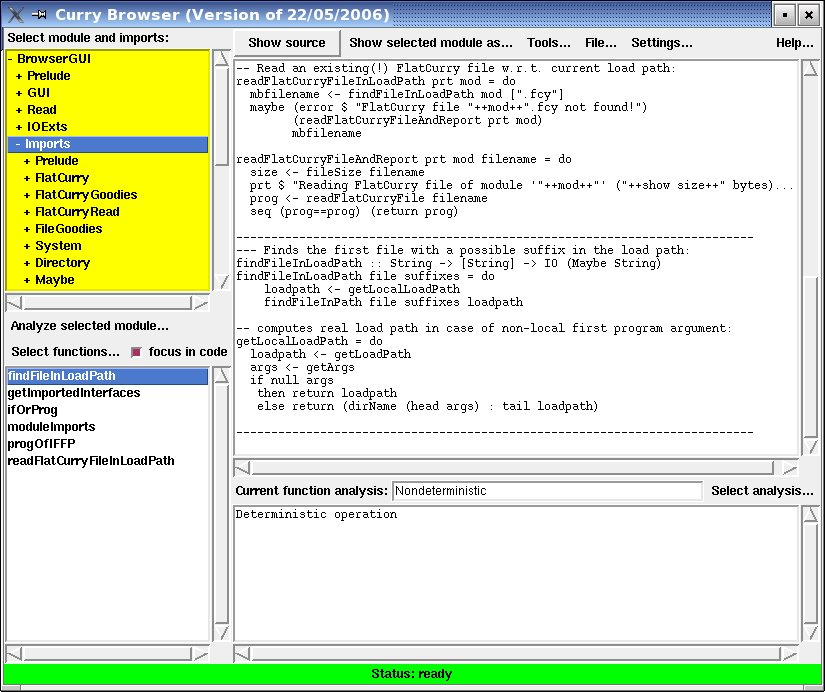
\includegraphics[scale=0.7]{currybrowser.jpg}
\end{center}
\caption{Snapshot of the main window of CurryBrowser\label{fig-currybrowser}}
\end{figure}
%
To get an impression of the use of \cb, Figure~\ref{fig-currybrowser}
shows a snapshot of its use on a particular application
(here: the implementation of \cb).
The upper list box in the left column shows the modules and their imports
in order to browse through the modules of an application.
Similarly to directory browsers, the list of imported modules of a module
can be opened or closed by clicking.
After selecting a module in the list of modules, its source code,
interface, or various other formats of the module can be shown
in the main (right) text area. For instance, one can show
pretty-printed versions of the intermediate flat programs (see below)
in order to see how local function definitions are translated by lambda lifting
\cite{Johnsson85}
or pattern matching is translated into case expressions \cite{Hanus97POPL,Wadler87}.
Since Curry is a language with parametric polymorphism and type inference,
programmers often omit the type signatures when defining functions.
Therefore, one can also view (and store) the selected module as source code where
missing type signatures are added.

Below the list box for selecting modules, there is a menu
(``Analyze selected module'') to analyze all functions
of the currently selected module at once. This is useful
to spot some functions of a module that could be problematic
in some application contexts, like functions that are impure (i.e., the result
depends on the evaluation time) or partially defined (i.e.,
not evaluable on all ground terms).
If such an analysis is selected,
the names of all functions are shown in the
lower list box of the left column (the ``function list'')
with prefixes indicating the properties of the individual functions.

The function list box can be also filled with functions
via the menu ``Select functions''. For instance, all functions
or only the exported functions defined in the currently selected
module can be shown there, or all functions from different modules
that are directly or indirectly called from
a currently selected function.
This list box is central to focus on a function in the
source code of some module or to analyze some function,
i.e., showing their properties. In order to focus on a function,
it is sufficient to check the ``focus on code'' button.
To analyze an individually selected function, one can
select an analysis from the list of available program analyses
(through the menu ``Select analysis'').
In this case, the analysis results are either shown
in the text box below the main text area
or visualized by separate tools, e.g., by a graph drawing tool for
visualizing call graphs.
Some analyses are local, i.e., they need only to consider the local definition
of this function (e.g., ``Calls directly,'' ``Overlapping rules,''
``Pattern completeness''),
where other analyses are global, i.e.,
they consider the definitions of all functions directly or indirectly called
by this function (e.g., ``Depends on,'' ``Solution complete,''
``Set-valued'').
%
Finally, there are a few additional tools integrated into \cb,
for instance, to visualize the import relation between all modules
as a dependency graph. These tools are available through the ``Tools'' menu.

More details about the use of \cb and all built-in analyses
are available through the ``Help'' menu of \cb.


\newpage

\section{CurryTest: A Tool for Testing Curry Programs}
\label{sec-currytest}

CurryTest\index{CurryTest}\index{testing programs}\index{program!testing}
is a simple tool in the PAKCS distribution to write
and run repeatable tests. CurryTest simplifies the task
of writing test cases for a module and executing them.
The tool is easy to use. Assume one has implemented a module \code{MyMod}
and wants to write some test cases to test its functionality,
making regression tests in future versions, etc.
For this purpose, there is a system library \code{Assertion}
(Section~\ref{Library:Assertion}) which
contains the necessary definitions for writing tests.
In particular, it exports an abstract polymorphic type \ccode{Assertion a}
together with the following operations:
\startprog
assertTrue      :: String -> Bool -> Assertion ()
assertEqual     :: String -> a -> a -> Assertion a
assertValues    :: String -> a -> [a] -> Assertion a
assertSolutions :: String -> (a->Success) -> [a] -> Assertion a
assertIO        :: String -> IO a -> a -> Assertion a
assertEqualIO   :: String -> IO a -> IO a -> Assertion a
\stopprog
The expression \ccode{assertTrue $s$ $b$}
is an assertion (named $s$) that the expression $b$ has the value \code{True}.
Similarly, the expression \ccode{assertEqual $s$ $e_1$ $e_2$}
asserts that the expressions $e_1$ and $e_2$
must be equal (i.e., \code{$e_1$==$e_2$} must hold),
the expression \ccode{assertValues $s$ $e$ $vs$} asserts
that $vs$ is the multiset of all values of $e$,
and the expression \ccode{assertSolutions $s$ $c$ $vs$} asserts
that the constraint abstraction $c$ has the multiset of solutions $vs$.
Furthermore, the expression \ccode{assertIO $s$ $a$ $v$}
asserts that the I/O action $a$ yields the value $v$ whenever it is
executed, and
the expression \ccode{assertEqualIO $s$ $a_1$ $a_2$}
asserts that the I/O actions $a_1$ and $a_2$ yields equal values.
The name $s$ provided as a first argument in each assertion
is used in the protocol produced by the test tool.

One can define a test program by importing the module
to be tested together with the module \code{Assertion} and defining
top-level functions of type \code{Assertion} in this module
(which must also be exported).
As an example, consider the following program
that can be used to test some list processing functions:
\startprog
\medskip
import List
import Assertion
\medskip
test1 = assertEqual     "++"     ([1,2]++[3,4]) [1,2,3,4]
\medskip
test2 = assertTrue      "all"    (all (<5) [1,2,3,4])
\medskip
test3 = assertSolutions "prefix" (\labs{}x -> let y free in  x\,++\,y =:= [1,2])
                                 [[],[1],[1,2]]
\medskip
\stopprog
For instance, \code{test1} asserts that the result of evaluating the
expression \code{([1,2]++[3,4])} is equal to \code{[1,2,3,4]}.

We can execute a test suite by the command\pindex{currytest}
\startprog
currytest testList
\stopprog
(\code{currytest} is a program stored in \code{$pakcshome$/bin}
where $pakcshome$ is the installation directory of PAKCS;
see Section~\ref{sec-general}).
In our example, \ccode{testList.curry} is the program containing the
definition of all assertions. This has the effect
that all exported top-level functions
of type \code{Assertion} are tested (i.e., the corresponding
assertions are checked) and the results
(\ccode{OK} or failure) are reported together with the name of each assertion.
%If failures occur, the complete test results are also
%written into a file named \ccode{testList.testlog}.''
For our example above, we obtain the following successful protocol:
\startprog
============================================================
Testing module "testList"...
OK: ++
OK: all
OK: prefix
All tests successfully passed.
============================================================
\stopprog
There is also a graphical interface that summarizes the results
more nicely.\footnote{Due to a bug in older versions of SICStus-Prolog,
it works only with SICStus-Prolog version 3.8.5 (or newer).}
In order to start this interface, one has to add the parameter
\ccode{--window} (or \ccode{-w}), e.g., executing a test suite by
\startprog
currytest --window testList
\stopprog
or
\startprog
currytest -w testList
\stopprog
A snapshot of the interface is shown in Figure~\ref{fig-currytest}.

\begin{figure}%[t]
\begin{center}
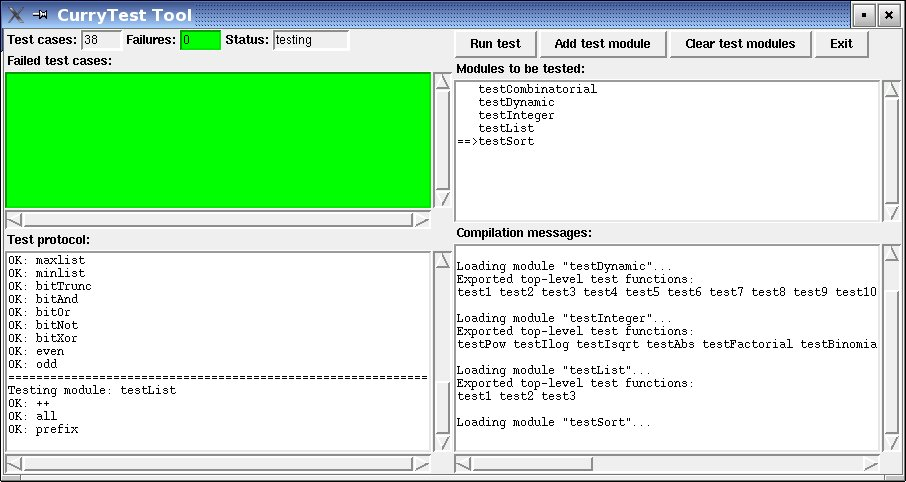
\includegraphics[scale=0.7]{currytest.jpg}
\end{center}
\caption{Snapshot of CurryTest's graphical interface\label{fig-currytest}}
\end{figure}


\newpage

\section{ERD2Curry: A Tool to Generate Programs from ER Specifications}
\label{sec-erd2curry}

ERD2Curry\index{ERD2Curry}\index{database programming}
is a tool to generate Curry code to access and manipulate data
persistently stored from
entity relationship diagrams.\index{entity relationship diagrams}
The idea of this tool is described in detail in
\cite{BrasselHanusMueller08PADL}.
Thus, we describe only the basic steps to use this tool
in the following.

If one creates an entity relationship diagram (ERD)
with the Umbrello UML Modeller, one has to store its
XML description in XMI format (as offered by Umbrello)
in a file, e.g., \ccode{myerd.xmi}.
This description can be compiled into a Curry program by the
command\pindex{erd2curry}
\startprog
erd2curry myerd.xmi
\stopprog
(\code{erd2curry} is a program stored in \code{$pakcshome$/bin}
where $pakcshome$ is the installation directory of PAKCS;
see Section~\ref{sec-general}).
If \code{MyData} is the name of the ERD, the Curry program file
\ccode{MyData.curry} is generated containing all the necessary
database access code as described in \cite{BrasselHanusMueller08PADL}.

If one does not want to use the Umbrello UML Modeller,
one can also create a textual description of the ERD
as a Curry term of type \code{ERD}
(w.r.t.\ the type definition given in module
\code{$pakcshome$/tools/erd2curry/ERD.curry})
and store it in some file, e.g., \ccode{myerd.term}.
This description can be compiled into a Curry program by the
command\pindex{erd2curry}
\startprog
erd2curry -t myerd.term
\stopprog
%
There is also the possibility to visualize an ERD term
as a graph with the graph visualization program \code{dotty}
(for this purpose, it might be necessary to adapt the definition
of the operation \code{dotCmd} in
\code{$pakcshome$/tools/erd2curry/ERD2Graph.curry}
according to your local environment).
This can be done by the command
\startprog
erd2curry -v myerd.term
\stopprog

\paragraph{Inclusion in the Curry application:}
To compile the generated database code, either
include the directory \code{$pakcshome$/tools/erd2curry}
into your Curry load path
(e.g., by setting  the environment variable
\ccode{CURRYPATH}\pindex{CURRYPATH}, see also Section~\ref{sec-modules})
or copy the file
\code{$pakcshome$/tools/erd2curry/ERDGeneric.curry}
into the directory of the generated database code.


\newpage

\section{UI: Declarative Programming of User Interfaces}
\label{sec-ui}

The PAKCS distribution contains a collection of libraries
to implement graphical user interfaces\index{user interface}
as well as web-based user interfaces
from declarative descriptions.
Exploiting these libraries, it is possible
to define the structure and functionality of a user interface
independent from the concrete technology.
Thus, a graphical user interface or a web-based user interface
can be generated from the same description by simply changing
the imported libraries.
This programming technique is described in detail in
\cite{HanusKluss09PADL}.

The libraries implementing these user interfaces are contained
in the directory
\startprog
$pakcshome$/tools/ui
\stopprog
Thus, in order to compile programs containing such user interface
specifications, one has to
include the directory \code{$pakcshome$/tools/ui}
into the Curry load path
(e.g., by setting  the environment variable
\ccode{CURRYPATH}\pindex{CURRYPATH}, see also Section~\ref{sec-modules}).
The directory
\startprog
$pakcshome$/tools/ui/examples
\stopprog
contains a few examples for such user interface specifications.


\newpage

\section{Preprocessing FlatCurry Files}
\label{sec-pakcspp}

The current parser allows to apply transformations on the intermediate
FlatCurry files after they are generated from the
corresponding Curry source file.
Currently, only the FlatCurry file corresponding to the main module
can be transformed.

A transformation can be specified as follows:
\begin{enumerate}
\item {\bf Options to \code{pakcs/bin/parsecurry}:}
\begin{description}
\item[\fbox{\code{--fpopt}}]\pindex{-fpopt}
Apply functional pattern optimization
(see \code{pakcs/tools/optimize/NonStrictOpt.curry} for details).

\item[\fbox{\code{--compact}}]\pindex{--compact}
Apply code compactification after parsing, i.e., transform the main
module and all its imported into one module and delete all
non-accessible functions.

\item[\fbox{\code{--compactexport}}]
Similar to \code{--compact} but delete all functions that are not accessible
from the exported functions of the main module.

\item[\fbox{\code{--compactmain:f}}]
Similar to \code{--compact} but delete all functions that are not accessible
from the function \ccode{f} of the main module.

\item[\fbox{\code{--fcypp cmd}}]\pindex{--fcypp}
Apply command \code{cmd} to the main module after parsing. This is useful to
integrate your own transformation into the compilation process.
Note that the command \ccode{cmd prog} should perform a transformation
on the FlatCurry file \code{prog.fcy}, i.e., it replaces the FlatCurry
file by a new one.
\end{description}

\item {\bf Setting the environment variable \code{FCYPP}:}\pindex{FCYPP}\\
For instance, setting \code{FCYPP} by
\startprog
export FCYPP="--fpopt"
\stopprog
will apply the functional pattern optimization if programs are compiled
and loaded in the PAKCS programming environment.


\item {\bf Putting options into the source code:}\pindex{PAKCS_OPTION_FCYPP}\\
If the source code contains a line with a comment of the form (the comment
must start at the beginning of the line)
\startprog
\{-\# PAKCS_OPTION_FCYPP <options> \#-\}
\stopprog
then the transformations specified by \code{<options>} are applied after
translating the source code into FlatCurry code. For instance,
the functional pattern optimization can be set by the comment
\startprog
\{-\# PAKCS_OPTION_FCYPP --fpopt \#-\}
\stopprog
in the source code. Note that this comment must be in a single line 
of the source program. If there are multiple lines containing such comments,
only the first one will be considered.
\end{enumerate}
\paragraph{Multiple options:}
Note that an arbitrary number of transformations can be specified
by the methods described above.
If several specifications for preprocessing FlatCurry files are used,
they are executed in the following order:
\begin{enumerate}
\item all transformations specified by the environemnt variable
\code{FCYPP} (from left to right)
\item all transformations specified as command line options of parsecurry
   (from left to right)
\item all transformations specified by a comment line in the source code
   (from left to right)
\end{enumerate}


\newpage

\section{Technical Problems}

Due to the fact that Curry is intended to implement
distributed systems (see Appendix~\ref{sec-ports}),
it might be possible that some technical problems
arise due to the use of sockets for implementing these
features. Therefore, this section gives some information
about the technical requirements of PAKCS and how to solve
problems due to these requirements.

There is one fixed port that is used by the implementation of PAKCS:
\begin{description}
\item[Port 8766:] This port is used by the
{\bf Curry Port Name Server} (CPNS) to implement symbolic names for
ports in Curry (see Appendix~\ref{sec-ports}).
If some other process uses this port on the machine,
the distribution facilities defined in the module \code{Ports}
(see Appendix~\ref{sec-ports}) cannot be used.
\end{description}
If these features do not work, you can try to find out
whether this port is in use by the shell command
\ccode{netstat -a | fgrep 8766} (or similar).

The CPNS is implemented as a demon listening on its port 8766
in order to serve requests about registering a new symbolic
name for a Curry port or asking the physical port number
of a Curry port. The demon will be automatically started for
the first time on a machine when a user compiles a program
using Curry ports. It can also be manually started and terminated by the
scripts \code{$pakcshome$/cpns/start} and
\code{$pakcshome$/cpns/stop}.
If the demon is already running, the command \code{$pakcshome$/cpns/start}
does nothing (so it can be always executed
before invoking a Curry program using ports).

If you detect any further technical problem,
please write to
\begin{center}
\code{mh@informatik.uni-kiel.de}
\end{center}

\newpage

\addcontentsline{toc}{section}{Bibliography}
\bibliography{manual}
\bibliographystyle{plain}

\newpage
\appendix

\section{Libraries of the PAKCS Distribution}
\label{sec:libraries}

{\setlength{\parindent}{0.0cm}

The PAKCS compiler system provides an extensive collection
of libraries for application programming.
The libraries for arithmetic constraints over real numbers,
finite domain constraints,
ports for concurrent and distributed programming, and
meta-programming by representing Curry programs in Curry
are described in the following subsection in more detail.
The complete set of libraries with all exported types and functions
are described in the further subsections.
For a more detailed online documentation of all libraries of PAKCS,
see \url{http://www.informatik.uni-kiel.de/~pakcs/lib/index.html}.

\subsection{Constraints, Ports, Meta-Programming}

\subsubsection{Arithmetic Constraints}

The primitive entities for the use of arithmetic constraints
are defined in the system module \code{CLPR}
(cf.\ Section~\ref{sec-modules}), i.e., in order to use them,
the program must contain the import declaration
\startprog
import CLPR
\stopprog
Floating point arithmetic is supported in PAKCS
via arithmetic constraints, i.e., the equational constraint
\ccode{2.3 +.~x =:= 5.5} is solved by binding \code{x} to \code{3.2}
(rather than suspending the evaluation of the addition,
as in corresponding constraints on integers like
\ccode{3+x=:=5}). All operations related to
floating point numbers are suffixed by \ccode{.}.
The following functions and constraints on floating point
numbers are supported in PAKCS:
\begin{description}
\item[\code{(+.)   :: Float -> Float -> Float}]~\\
Addition on floating point numbers.
\item[\code{(-.)   :: Float -> Float -> Float}]~\\
Subtraction on floating point numbers.
\item[\code{(*.)   :: Float -> Float -> Float}]~\\
Multiplication on floating point numbers.
\item[\code{(/.)   :: Float -> Float -> Float}]~\\
Division on floating point numbers.
\item[\code{(<.)   :: Float -> Float -> Success}]~\\
Comparing two floating point numbers with the ``less than'' relation.
\item[\code{(>.)   :: Float -> Float -> Success}]~\\
Comparing two floating point numbers with the ``greater than'' relation.
\item[\code{(<=.)  :: Float -> Float -> Success}]~\\
Comparing two floating point numbers with the ``less than or equal'' relation.
\item[\code{(>=.)  :: Float -> Float -> Success}]~\\
Comparing two floating point numbers with the ``greater than or equal''
relation.
\item[\code{i2f    :: Int -> Float}]~\\
Converting an integer number into a floating point number.
\end{description}
As an example, consider a constraint \code{mortgage}
which relates the principal \code{p},
the lifetime of the mortgage in months \code{t},
the monthly interest rate \code{ir},
the monthly repayment \code{r},
and the outstanding balance at the end of the lifetime \code{b}.
The financial calculations
can be defined by the following two rules in Curry (the second rule
describes the repeated accumulation of the interest):
\startprog
~
import CLPR
~
mortgage p t ir r b | t >. 0.0 \& t <=. 1.0  --lifetime not more than 1 month?
                    =  b =:= p *. (1.0 +. t *. ir) -. t*.r \vspace{1ex}
mortgage p t ir r b | t >. 1.0               --lifetime more than 1 month?
                    =  mortgage (p *. (1.0+.ir)-.r) (t-.1.0) ir r b
~
\stopprog
Then we can calculate the monthly payment for paying back
a loan of \$100,000 in 15 years with a monthly interest rate of 1\%
by solving the goal
\startprog
mortgage 100000.0 180.0 0.01 r 0.0
\stopprog
which yields the solution \code{r=1200.17}.

Note that only linear arithmetic equalities or inequalities
are solved by the constraint solver. Non-linear constraints
like \ccode{x *.~x =:= 4.0} are suspended until they become
linear.


\subsubsection{Finite Domain Constraints}

Finite domain constraints are constraints where all variables
can only take a finite number of possible values.
For simplicity, the domain of finite domain variables are
identified with a subset of the integers, i.e., the type
of a finite domain variable is \code{Int}. The arithmetic
operations related to finite domain variables are suffixed by \ccode{\#}.
The following functions and constraints for finite domain constraint solving
are currently supported in PAKCS:\footnote{Note that
this library is based on the corresponding library of SICStus-Prolog
but does not implement the complete functionality of the SICStus-Prolog library.
However, using the PAKCS interface for external functions (see
Appendix~\ref{sec-external-functions}), it is relatively
easy to provide the complete functionality.}

\begin{description}
\item[\code{domain :: [Int] -> Int -> Int -> Success}]~\\
The constraint \ccode{domain [$x_1,\ldots,x_n$] $l$ $u$}
is satisfied if the domain of all variables $x_i$ is the interval $[l,u]$.
\item[\code{(+\#)   :: Int -> Int -> Int}]~\\
Addition on finite domain values.
\item[\code{(-\#)   :: Int -> Int -> Int}]~\\
Subtraction on finite domain values.
\item[\code{(*\#)   :: Int -> Int -> Int}]~\\
Multiplication on finite domain values.
\item[\code{(=\#)   :: Int -> Int -> Success}]~\\
Equality of finite domain values.
\item[\code{(/=\#)  :: Int -> Int -> Success}]~\\
Disequality of finite domain values.
\item[\code{(<\#)   :: Int -> Int -> Success}]~\\
``less than'' relation on finite domain values.
\item[\code{(<=\#)  :: Int -> Int -> Success}]~\\
``less than or equal'' relation on finite domain values.
\item[\code{(>\#)   :: Int -> Int -> Success}]~\\
``greater than'' relation on finite domain values.
\item[\code{(>=\#)  :: Int -> Int -> Success}]~\\
``greater than or equal'' relation on finite domain values.
\item[\code{sum :: [Int] -> (Int -> Int -> Success) -> Int -> Success}]~\\
The constraint \ccode{sum [$x_1,\ldots,x_n$] $op$ $x$}
is satisfied if all $x_1+\cdots + x_n \mathrel{op} x$ is satisfied,
where $op$ is one of the above finite domain constraint relations
(e.g., \ccode{=\#}).
\item[\code{scalar_product :: [Int] -> [Int] -> (Int -> Int -> Success) -> Int -> Success}]~\\
The constraint \ccode{scalar_product [$c_1,\ldots,c_n$] [$x_1,\ldots,x_n$] $op$ $x$}
is satisfied if all $c_1 x_1+\cdots + c_n x_n \mathrel{op} x$ is satisfied,
where $op$ is one of the above finite domain constraint relations.
\item[\code{count :: Int -> [Int] -> (Int -> Int -> Success) -> Int -> Success}]~\\
The constraint \ccode{count $k$ [$x_1,\ldots,x_n$] $op$ $x$}
is satisfied if all $k \mathrel{op} x$ is satisfied,
where $n$ is the number of the $x_i$ that are equal to $k$ and
$op$ is one of the above finite domain constraint relations.
\item[\code{all_different :: [Int] -> Success}]~\\
The constraint \ccode{all_different [$x_1,\ldots,x_n$]}
is satisfied if all $x_i$ have pairwise different values.
\item[\code{labeling :: [LabelingOption] -> [Int] -> Success}]~\\
The constraint \ccode{labeling $os$ [$x_1,\ldots,x_n$]}
non-deterministically instantiates all $x_i$ to the values
of their domain according to the options $os$ (see the module documentation
for further details about these options).
\end{description}
These entities are defined in the system module \code{CLPFD}
(cf.\ Section~\ref{sec-modules}), i.e., in order to use it,
the program must contain the import declaration
\startprog
import CLPFD
\stopprog
As an example, consider the classical \ccode{send+more=money} problem
where each letter must be replaced by a different digit such that this
equation is valid and there are no leading zeros.
The usual way to solve finite domain constraint problems
is to specify the domain of the involved variables followed
by a specification of the constraints and the labeling
of the constraint variables in order to start the search for solutions.
Thus, the \ccode{send+more=money} problem can be solved as follows:
\startprog
~
import CLPFD
~
smm l =
        l =:= [s,e,n,d,m,o,r,y] \&
        domain l 0 9 \&
        s >\# 0 \&
        m >\# 0 \&
        all_different l  \&
                         1000 *\# s +\# 100 *\# e +\# 10 *\# n +\# d
        +\#               1000 *\# m +\# 100 *\# o +\# 10 *\# r +\# e
        =\# 10000 *\# m +\# 1000 *\# o +\# 100 *\# n +\# 10 *\# e +\# y \&
        labeling [FirstFail] l
        where s,e,n,d,m,o,r,y free
~
\stopprog
Then we can solve this problem by evaluating the goal
\ccode{smm [s,e,n,d,m,o,r,y]} which yields the unique solution
\code{\{s=9,e=5,n=6,d=7,m=1,o=0,r=8,y=2\}}.


\subsubsection{Ports: Distributed Programming in Curry}
\label{sec-ports}

To support the development of concurrent and distributed applications,
PAKCS supports internal and external ports\index{ports} as
described in \cite{Hanus99PPDP}.
Since \cite{Hanus99PPDP} contains a detailed description of this
concept together with various programming examples, we only summarize here
the functions and constraints supported for ports in PAKCS.

The basic datatypes, functions, and constraints for ports
are defined in the system module \code{Ports}
(cf.\ Section~\ref{sec-modules}), i.e., in order to use ports,
the program must contain the import declaration
\startprog
import Ports
\stopprog
This declaration includes the following entities in the program:
\begin{description}
\item[\code{Port a}\pindex{Port}]~\\
This is the datatype of a port to which one can send messages of type \code{a}.

\item[\code{openPort :: Port a -> [a] -> Success}]~\\
The constraint \ccode{openPort p s}\pindex{openPort}
establishes a new \emph{internal port}
\code{p} with an associated message stream \code{s}. \code{p} and \code{s} must be
unbound variables,
otherwise the constraint fails (and causes a runtime error).

\item[\code{send :: a -> Port a -> Success}]~\\
The constraint \ccode{send m p}\pindex{send}
is satisfied if \code{p} is constrained
to contain the message \code{m}, i.e., \code{m} will be sent to the port
\code{p} so that it appears in the corresponding stream.

\item[\code{doSend :: a -> Port a -> IO ()}]~\\
The I/O action \ccode{doSend m p}\pindex{doSend} solves the constraint
\ccode{send m p} and returns nothing.

\item[\code{openNamedPort :: String -> IO [a]}]~\\
The I/O action \ccode{openNamedPort n}\pindex{openNamedPort}
opens a new \emph{external port} with
symbolic name \code{n} and returns the associated stream of messages.

\item[\code{connectPort :: String -> IO (Port a)}]~\\
The I/O action \ccode{connectPort n}\pindex{connectPort}
returns a port with symbolic name
\code{n} (i.e., \code{n} must have the form ``\emph{portname@machine})
to which one can send messages by the \code{send} constraint.
Currently, no dynamic type checking is done for external ports,
i.e., sending messages of the wrong type to a port might lead to
a failure of the receiver.
\end{description}

\paragraph{Restrictions:}
Every expression, possibly containing logical variables, can be sent to
a port. However, as discussed in \cite{Hanus99PPDP},
port communication is strict, i.e., the expression is
evaluated to normal form before sending it by the
constraint \code{send}. Furthermore, if messages containing
logical variables are sent to \emph{external ports},
the behavior is as follows:
\begin{enumerate}
\item The sender waits until all logical variables in the message
have been bound by the receiver.
\item The binding of a logical variable received by a process
is sent back to the sender of this logical variable only if
it is bound to a \emph{ground} term, i.e., as long as the binding contains
logical variables, the sender is not informed about the binding
and, therefore, the sender waits.
\end{enumerate}

\paragraph{External ports on local machines:}
The implementation of external ports assumes that the
host machine running the application is connected to the Internet
(i.e., it uses the standard IP address of the host machine
for message sending). If this is not the case and the application
should be tested by using external ports only on the local host
without a connection to the Internet,
the environment variable \ccode{PAKCS_LOCALHOST}\pindex{PAKCS_LOCALHOST}
must be set to \ccode{yes}
\emph{before PAKCS system is started}.
In this case, the IP address \code{127.0.0.1} and the hostname
\ccode{localhost} are used for identifying the local machine.

\paragraph{Selection of Unix sockets for external ports:}
The implementation of ports uses sockets to communicate
messages sent to external ports.
Thus, if a Curry program uses the
I/O action \code{openNamedPort}\pindex{openNamedPort}
to establish an externally visible server,
PAKCS selects a Unix socket for the port communication.
Usually, a free socket is selected by the operating system.
If the socket number should be fixed in an application (e.g.,
because of the use of firewalls\index{firewall} that allow only
communication over particular sockets), then one
can set the environment variable \ccode{PAKCS_SOCKET}\pindex{PAKCS_SOCKET}
to a distinguished socket number before the PAKCS system is started.
This has the effect that PAKCS uses only this socket
number for communication (even for several external ports
used in the same application program).

\paragraph{Debugging:}
To debug distributed systems,
it is sometimes helpful to see all messages sent to external ports.
This is supported by the environment variable
\ccode{PAKCS_TRACEPORTS}.\pindex{PAKCS_TRACEPORTS}
If this variable is set to \ccode{yes}
\emph{before the PAKCS system is started}, then all
connections to external ports and all
messages sent and received on external ports are
printed on the standard error stream.


\subsubsection{AbstractCurry and FlatCurry: Meta-Programming in Curry}
\label{sec-flatcurry}

\index{AbstractCurry}
\index{FlatCurry}
To support meta-programming, i.e., the manipulation of Curry programs
in Curry, there are system modules \code{FlatCurry} and \code{AbstractCurry}
(stored in the directory \ccode{$pakcshome$/lib/meta})
which define datatypes for the representation
of Curry programs.
\code{AbstractCurry} is a more direct representation of a Curry program,
whereas \code{FlatCurry} is a simplified representation
where local function definitions are replaced by global definitions
(i.e., lambda lifting has been performed) and pattern matching
is translated into explicit case/or expressions.
Thus, \code{FlatCurry} can be used for more back-end oriented
program manipulations (or, for writing new back ends for Curry),
whereas \code{AbstractCurry} is intended for manipulations of
programs that are more oriented towards the source program.

Both modules contain predefined I/O actions to read programs
in the \code{AbstractCurry} (\code{readCurry}\pindex{readCurry})
or \code{FlatCurry}
(\code{readFlatCurry}\pindex{readFlatCurry}) format.
These actions parse the corresponding source program and return
a data term representing this program (according to the definitions
in the modules \code{AbstractCurry} and \code{FlatCurry}).

Since all datatypes are explained in detail in these modules,
we refer to the online documentation\footnote{%
\url{http://www.informatik.uni-kiel.de/~pakcs/lib/CDOC/FlatCurry.html} and
\url{http://www.informatik.uni-kiel.de/~pakcs/lib/CDOC/AbstractCurry.html}}
of these modules.

As an example, consider a program file \ccode{test.curry}
containing the following two lines:
\startprog
rev []     = []
rev (x:xs) = (rev xs) ++ [x]
\stopprog
Then the I/O action \code{(FlatCurry.readFlatCurry "test")} returns the
following term:
\startprog
 (Prog "test"
  ["Prelude"]
  []
  [Func ("test","rev") 1 Public
        (FuncType (TCons ("Prelude","[]") [(TVar 0)])
                  (TCons ("Prelude","[]") [(TVar 0)]))
        (Rule [0]
           (Case Flex (Var 0)
              [Branch (Pattern ("Prelude","[]") [])
                  (Comb ConsCall ("Prelude","[]") []),
               Branch (Pattern ("Prelude",":") [1,2])
                  (Comb FuncCall ("Prelude","++")
                        [Comb FuncCall ("test","rev") [Var 2],
                         Comb ConsCall ("Prelude",":")
                              [Var 1,Comb ConsCall ("Prelude","[]") []]
                        ])
              ]))]
  []
 )
\stopprog


%%%%%%%%%%%%%%%%%%%%%%%%%%%%%%%%%%%%%%%%%%%%%%%%%%%%%%%%%%%%%%%%%%%%%%%%%
% Definitions in order to LaTeX documents generated by "currydoc --tex"
%%%%%%%%%%%%%%%%%%%%%%%%%%%%%%%%%%%%%%%%%%%%%%%%%%%%%%%%%%%%%%%%%%%%%%%%%

\newcommand{\currymodule}[1]{\subsubsection{Library #1}\label{Library:#1}}
\newcommand{\currytypesstart}{\subsubsection*{Exported types:}}
\newcommand{\currytypesstop}{}
\newcommand{\currytypesynstart}[2]{{\tt type #2}\pindex{#1} \begin{quote}}
\newcommand{\currytypesynstop}{\end{quote}}
\newcommand{\currydatastart}[1]{{\tt data #1}\pindex{#1} \begin{quote}}
\newcommand{\currydatacons}{\end{quote}%
\begin{itemize}\item[] \hspace{-4ex}\emph{Exported constructors:}}
\newcommand{\currydatastop}{\end{itemize}}
\newcommand{\curryconsstart}[2]{\item {\tt #1~::~#2}\par}
\newcommand{\curryfuncstart}{\subsubsection*{Exported functions:}}
\newcommand{\curryfuncstop}{}
\newcommand{\curryfunctionstart}[2]{#2\pindex{#1}\begin{quote}}
\newcommand{\curryfunctionstop}{\end{quote}}
\newcommand{\curryfuncsig}[2]{{\tt #1~::~#2}}


\subsection{General Libraries}

\input{lib/AllSolutions}
\input{lib/Assertion}
\input{lib/Char}
\input{lib/CLPFD}
\input{lib/CLPR}
\input{lib/CLPB}
\input{lib/Combinatorial}
\input{lib/Constraint}
\input{lib/CSV}
\input{lib/Database}
\input{lib/DaVinci}
\input{lib/Directory}
\input{lib/Dynamic}
\input{lib/FileGoodies}
\input{lib/Float}
\input{lib/Global}
\input{lib/GlobalVariable}
\input{lib/GUI}
\input{lib/Integer}
\input{lib/IO}
\input{lib/IOExts}
\input{lib/JavaScript}
\input{lib/KeyDatabase}
\input{lib/KeyDatabaseSQLite}
\input{lib/KeyDB}
\input{lib/List}
\input{lib/Maybe}
\input{lib/NamedSocket}
\input{lib/Parser}
\input{lib/Ports}
\input{lib/Pretty}
\input{lib/Profile}
\input{lib/PropertyFile}
\input{lib/Read}
\input{lib/ReadNumeric}
\input{lib/ReadShowTerm}
\input{lib/SetFunctions}
\input{lib/Socket}
\input{lib/System}
\input{lib/Time}
%\input{lib/Tk}
\input{lib/Unsafe}


\subsection{Data Structures and Algorithms}

\input{lib/Array}
\input{lib/Dequeue}
\input{lib/FiniteMap}
\input{lib/GraphInductive}
\input{lib/Random}
\input{lib/RedBlackTree}
\input{lib/SetRBT}
\input{lib/Sort}
\input{lib/TableRBT}
\input{lib/Traversal}

\subsection{Libraries for Web Applications}

\input{lib/CategorizedHtmlList}
\input{lib/HTML}
\input{lib/HtmlParser}
\input{lib/Mail}
\input{lib/Markdown}
\input{lib/WUI}
\input{lib/URL}
\input{lib/XML}
\input{lib/XmlConv}

\subsection{Libraries for Meta-Programming}

\input{lib/AbstractCurry}
\input{lib/AbstractCurryPrinter}
\input{lib/CompactFlatCurry}
\input{lib/CurryStringClassifier}
\input{lib/FlatCurry}
\input{lib/FlatCurryGoodies}
\input{lib/FlatCurryRead}
\input{lib/FlatCurryShow}
\input{lib/FlatCurryTools}
\input{lib/FlatCurryXML}
\input{lib/FlexRigid}
\input{lib/PrettyAbstract}

} % end setlength parindent

\newpage

\input{markdown_syntax}

\newpage

\begin{figure}%[t]
\begin{center}
 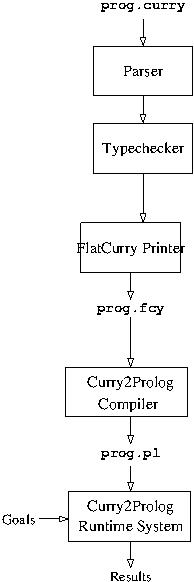
\includegraphics[scale=0.85]{pakcs_overview.jpg}
\end{center}\vspace{-5ex}
\caption{Overview of PAKCS\label{fig-pakcs}}
\end{figure}

\section{Overview of the PAKCS Distribution}

A schematic overview of the various components contained in
the distribution of PAKCS and the
translation process of programs inside PAKCS is shown in
Figure~\ref{fig-pakcs} on page~\pageref{fig-pakcs}.
In this figure, boxes denote different components of PAKCS
and names in boldface denote files containing
various intermediate representations during the translation
process (see Section~\ref{sec-auxfiles} below).
The PAKCS distribution contains a front end for reading (parsing and
type checking) Curry programs that can be also used by
other Curry implementations.
The back end (formerly known as ``Curry2Prolog''\index{Curry2Prolog})
compiles Curry programs into Prolog programs.
It also support constraint solvers for
arithmetic constraints over real numbers and finite domain constraints,
and further libraries for GUI programming, meta-programming etc.
Currently, it does not implement encapsulated search in full generality
(only a strict version of \code{findall} is supported),
and concurrent threads are not executed in a fair manner.


\newpage

\section{Auxiliary Files}
\label{sec-auxfiles}

During the translation and execution of a Curry program with PAKCS,
various intermediate representations of the source program are created
and stored in different files which are shortly explained in this section.
If you use the PAKCS, it is not necessary to know about
these auxiliary files because they are automatically generated
and updated. You should only remember the command for deleting
all auxiliary files (\ccode{cleancurry}, see Section~\ref{sec-general})
to clean up your directories.

The various components of PAKCS create
the following auxiliary files.
\begin{description}
\item[\code{prog.fcy}:] This file contains the Curry program
in the so-called ``FlatCurry'' representation where all functions are global
(i.e., lambda lifting has been performed) and pattern matching
is translated into explicit case/or expressions
(compare Appendix~\ref{sec-flatcurry}).
This representation might be useful for other back ends and
compilers for Curry and is the basis doing meta-programming in Curry.
This file is implicitly
generated when a program is read by PAKCS.
It can be also explicitly generated by the command\pindex{parsecurry}
\startprog
parsecurry --flat prog
\stopprog
The FlatCurry representation of a Curry program is usually
generated by the front-end after parsing, type checking and eliminating
local declarations.
If $dir$ is the directory where the Curry program is stored,
the corresponding FlatCurry program is stored in the directory
\ccode{$dir$/.curry}.

\item[\code{prog.fint}:] This file contains the interface
of the program in the so-called ``FlatCurry'' representation,
i.e., it is similar to \code{prog.fcy} but contains only exported
entities and the bodies of all functions omitted (i.e., ``external'').
This representation is useful for providing a fast access
to module interfaces.
This file is implicitly generated by the command\pindex{parsecurry}
\startprog
parsecurry --flat prog
\stopprog
and stored in the same directory as \code{prog.fcy}.

\item[\code{prog.pl}:] This file contains a Prolog program
as the result of translating the Curry program with PAKCS.
If $dir$ is the directory where the Curry program is stored,
the corresponding Prolog program is stored in the directory
\ccode{$dir$/.curry/.pakcs}.

\item[\code{prog.po}:] This file contains the Prolog program
\code{prog.pl} in an intermediate format for faster loading.
This file is stored in the same directory as \code{prog.pl}.

\item[\code{prog.state}:] This file contains the saved state
after compiling and saving a program with PAKCS
(see Section~\ref{sec-use-curry2prolog}).

\end{description}


\newpage


\section{Changing the Prelude or System Modules}

The standard prelude, which is automatically imported into each Curry program,
and all system modules containing datatypes and functions
useful for application programming
(cf.\ Appendix~\ref{sec:libraries})
are stored in the system module directory \ccode{$pakcshome$/lib}
(and its subdirectories).
If you change any of these modules,
you have to recompile the complete system by
executing \code{make} in the directory $pakcshome$.



\newpage

\section{External Functions}
\label{sec-external-functions}

\index{function!external}\index{external function}
Currently, PAKCS has no general interface to external functions.
Therefore, if a new external function should be added
to the system, this function must be declared as \code{external}
in the Curry source code
and then an implementation for this external function
must be inserted in the corresponding back end.
An external function is defined as follows in the Curry source code:
\begin{enumerate}
\item
Add a type declaration for the external function somewhere
in the body of the appropriate file (usually, the prelude
or some system module).
\item
For external functions it is not allowed to define any
rule since their semantics is determined by an external implementation.
Instead of the defining rules, you have to write
\startprog
f external
\stopprog
somewhere in the file containing the type declaration for 
the external function \code{f}.
\end{enumerate}
For instance, the addition on integers can be declared as
an external function as follows:
\startprog
(+) :: Int -> Int -> Int
(+) external
\stopprog
The further modifications to be done for an inclusion of
an external function has to be done in the back end.
A new external function is added to the back end of PAKCS
by informing the compiler about the existence of an external function
and adding an implementation of this function in the run-time
system. Therefore, the following items must be added
in the PAKCS compiler system:
\begin{enumerate}
\item
If the Curry module \code{Mod} contains external functions,
there must be a file named \code{Mod.prim_c2p} containing the
specification of these external functions. The contents of this file
is in XML format and has the following general structure:\footnote{%
\url{http://www.informatik.uni-kiel.de/~pakcs/primitives.dtd} contains a DTD
describing the exact structure of these files.}
\startprog
<primitives>
  \emph{specification of external function $f_1$}
  \ldots
  \emph{specification of external function $f_n$}
</primitives>
\stopprog
The specification of an external function $f$
with arity $n$ has the form
\startprog
<primitive name="$f$" arity="$n$">
  <library>lib</library>
  <entry>pred</entry>
</primitive>
\stopprog
where \code{lib} is the Prolog library (stored in the directory of the
Curry module or in the global directory
\code{$pakcshome$/curry2prolog/lib_src}) containing the code implementing this
function and \code{pred} is a predicate name in this library
implementing this function. Note that the function $f$ must be
declared in module \code{Mod}: either as an external function
or defined in Curry by equations. In the latter case,
the Curry definition is not translated but calls to this function
are redirected to the Prolog code specified above.

Furthermore, the list of specifications can also contain entries of the form
\startprog
<ignore name="$f$" arity="$n$" />
\stopprog
for functions $f$ with arity $n$ that are declared in module \code{Mod}
but should be ignored for code generation, e.g., since they are
never called w.r.t.\ to the current implementation of external functions.
For instance, this is useful when functions that can
be defined in Curry should be (usually more efficiently) are implemented
as external functions.

Note that the arguments are passed in their current (possibly unevaluated) form.
Thus, if the external function requires the arguments to be evaluated
in a particular form, this must be done before calling the external function.
For instance, the external function for adding two integers
requires that both arguments must be evaluated to non-variable head normal form
(which is identical to the ground constructor normal form). Therefore,
the function \ccode{+} is specified in the prelude by
\startprog
(+)   :: Int -> Int -> Int
x + y = (prim_Int_plus \$\# y) \$\# x
\medskip
prim_Int_plus :: Int -> Int -> Int
prim_Int_plus external
\stopprog
where \code{prim_Int_plus} is the actual external function implementing
the addition on integers. Consequently, the specification file
\code{Prelude.prim_c2p} has an entry of the form
\startprog
<primitive name="prim_Int_plus" arity="2">
  <library>prim_standard</library>
  <entry>prim_Int_plus</entry>
</primitive>
\stopprog
where the Prolog library \code{prim_standard.pl} contains the Prolog code
implementing this function.

\item
For most external functions, a \emph{standard interface} is
generated by the compiler so that an $n$-ary function can be
implemented by an $(n+1)$-ary predicate where the last argument must
be instantiated to the result of evaluating the function.  The
standard interface can be used if all arguments are ensured to be
fully evaluated (e.g., see definition of \code{(+)} above) and no
suspension control is necessary, i.e., it is ensured that the
external function call does not suspend for all arguments.
Otherwise, the raw interface (see below) must be used.  For
instance, the Prolog code implementing \code{prim_Int_plus}
contained in the Prolog library \code{prim_standard.pl} is as
follows (note that the arguments of \code{(+)} are passed in reverse
order to \code{prim_Int_plus} in order to ensure a left-to-right
evaluation of the original arguments by the calls to \code{(\$\#)}):
\startprog
prim_Int_plus(Y,X,R) :- R is X+Y.
\stopprog

\item
The \emph{standard interface for I/O actions}, i.e., external functions
with result type \code{IO~a}, assumes that the I/O action
is implemented as a predicate (with a possible side effect)
that instantiates the last argument to the returned value of type \ccode{a}.
For instance, the primitive predicate \code{prim_getChar}
implementing prelude I/O action \code{getChar}
can be implemented by the Prolog code
\startprog
prim_getChar(C) :- get_code(N), char_int(C,N).
\stopprog
where \code{char_int} is a predicate relating the internal
Curry representation of a character with its ASCII value.

\item
If some arguments passed to the external functions are not fully evaluated
or the external function might suspend, the implementation must follow
the structure of the PAKCS run-time system by using
the \emph{raw interface}. In this case, the name of the external entry
must be suffixed by \ccode{[raw]} in the \code{prim_c2p} file.
For instance, if we want to use the raw interface for the external function
\code{prim_Int_plus},
the specification file \code{Prelude.prim_c2p} must have an entry of the form
\startprog
<primitive name="prim_Int_plus" arity="2">
  <library>prim_standard</library>
  <entry>prim_Int_plus[raw]</entry>
</primitive>
\stopprog
In the raw interface, the actual implementation of an $n$-ary external function consists
of the definition of an $(n+3)$-ary predicate $pred$.
The first $n$ arguments are the corresponding actual arguments.
The $(n+1)$-th argument is a free variable which must be
instantiated to the result of the function call after
successful execution. The last two arguments
control the suspension behavior of the function
(see \cite{AntoyHanus00FROCOS} for more details):
The code for the predicate $pred$
should only be executed when the $(n+2)$-th argument
is not free, i.e., this predicate has always the
SICStus-Prolog block declaration
\startprog
?- block $pred$(?,\ldots,?,-,?).
\stopprog
In addition, typical external functions should suspend
until the actual arguments are instantiated. This can be ensured
by a call to \code{ensureNotFree} or \code{(\$\#)}
before calling the external function. Finally, the
last argument (which is a free variable at call time)
must be unified with the $(n+2)$-th argument
after the function call is successfully evaluated
(and does not suspend). Additionally, the actual (evaluated) arguments
must be dereferenced before they are accessed.
Thus, an implementation
of the external function for adding integers is as follows in the raw interface:
\startprog
?- block prim_Int_plus(?,?,?,-,?).
prim_Int_plus(RY,RX,Result,E0,E) :-
     deref(RX,X), deref(RY,Y), Result is X+Y, E0=E.
\stopprog
Here, \code{deref} is a predefined predicate for dereferencing the
actual argument into a constant (and \code{derefAll} for dereferencing
complex structures).
\end{enumerate}
%
The Prolog code implementing the external functions must be accessible to the run-time
system of PAKCS by putting it into the directory containing the corresponding
Curry module or into the system directory
\code{$pakcshome$/curry2prolog/lib_src}.
Then it will be automatically loaded into the run-time environment
of each compiled Curry program.

Note that arbitrary functions implemented in C or Java can be connected to
PAKCS by using the corresponding interfaces of underlying Prolog system.


\newpage
\addcontentsline{toc}{section}{Index}
\printindex


\end{document}

\section{UI: Declarative Programming of User Interfaces}
\label{sec-ui}

The \CYS distribution contains a collection of libraries
to implement graphical user interfaces\index{user interface}
as well as web-based user interfaces
from declarative descriptions.
Exploiting these libraries, it is possible
to define the structure and functionality of a user interface
independent from the concrete technology.
Thus, a graphical user interface or a web-based user interface
can be generated from the same description by simply changing
the imported libraries.
This programming technique is described in detail in
\cite{HanusKluss09PADL}.

The libraries implementing these user interfaces are contained
in the directory
\begin{curry}
$\cyshome$/tools/ui
\end{curry}
Thus, in order to compile programs containing such user interface
specifications, one has to
include the directory \code{\cyshome/tools/ui}
into the Curry load path
(e.g., by setting  the environment variable
\ccode{CURRYPATH}\pindex{CURRYPATH}, see also Section~\ref{sec-modules}).
The directory
\begin{curry}
$\cyshome$/tools/ui/examples
\end{curry}
contains a few examples for such user interface specifications.

%%% Local Variables: 
%%% mode: latex
%%% TeX-master: "manual"
%%% End: 

\section{Preprocessing FlatCurry Files}
\label{sec-pakcspp}

After the invocation of the Curry front end to parse
Curry programs and translate them into the intermediate FlatCurry
representation, one can apply transformations on the FlatCurry files
before they are passed to the back end which translates
the FlatCurry files into Prolog code.
These transformations are invoked by the FlatCurry preprocessor
\code{pakcs/bin/fycpp}.\pindex{fcypp}
Currently, only the FlatCurry file corresponding to the main module
can be transformed.

A transformation can be specified as follows:
\begin{enumerate}
\item {\bf Options to \code{pakcs/bin/fcypp}:}
\begin{description}
\item[\fbox{\code{--fpopt}}]\pindex{-fpopt}
Apply functional pattern optimization
(see \code{pakcs/tools/optimize/NonStrictOpt.curry} for details).

\item[\fbox{\code{--compact}}]\pindex{--compact}
Apply code compactification after parsing, i.e., transform the main
module and all its imported into one module and delete all
non-accessible functions.

\item[\fbox{\code{--compactexport}}]
Similar to \code{--compact} but delete all functions that are not accessible
from the exported functions of the main module.

\item[\fbox{\code{--compactmain:f}}]
Similar to \code{--compact} but delete all functions that are not accessible
from the function \ccode{f} of the main module.

\item[\fbox{\code{--fcypp cmd}}]\pindex{--fcypp}
Apply command \code{cmd} to the main module after parsing. This is useful to
integrate your own transformation into the compilation process.
Note that the command \ccode{cmd prog} should perform a transformation
on the FlatCurry file \code{prog.fcy}, i.e., it replaces the FlatCurry
file by a new one.
\end{description}

\item {\bf Setting the environment variable \code{FCYPP}:}\pindex{FCYPP}\\
For instance, setting \code{FCYPP} by
\begin{curry}
export FCYPP="--fpopt"
\end{curry}
will apply the functional pattern optimization if programs are compiled
and loaded in the \CYS programming environment.

\item {\bf Putting options into the source code:}\pindex{PAKCS_OPTION_FCYPP}\\
If the source code contains a line with a comment of the form (the comment
must start at the beginning of the line)
\begin{curry}
{-# PAKCS_OPTION_FCYPP <options> #-}
\end{curry}
then the transformations specified by \code{<options>} are applied after
translating the source code into FlatCurry code. For instance,
the functional pattern optimization can be set by the comment
\begin{curry}
{-# PAKCS_OPTION_FCYPP --fpopt #-}
\end{curry}
in the source code. Note that this comment must be in a single line 
of the source program. If there are multiple lines containing such comments,
only the first one will be considered.
\end{enumerate}
\paragraph{Multiple options:}
Note that an arbitrary number of transformations can be specified
by the methods described above.
If several specifications for preprocessing FlatCurry files are used,
they are executed in the following order:
\begin{enumerate}
\item all transformations specified by the environemnt variable
\code{FCYPP} (from left to right)
\item all transformations specified as command line options of \code{fcypp}
   (from left to right)
\item all transformations specified by a comment line in the source code
   (from left to right)
\end{enumerate}


%%% Local Variables: 
%%% mode: latex
%%% TeX-master: "manual"
%%% End: 

\section{Technical Problems}

Due to the fact that Curry is intended to implement
distributed systems (see Appendix~\ref{sec-ports}),
it might be possible that some technical problems
arise due to the use of sockets for implementing these
features. Therefore, this section gives some information
about the technical requirements of \CYS and how to solve
problems due to these requirements.

There is one fixed port that is used by the implementation of \CYS:
\begin{description}
\item[Port 8766:] This port is used by the
{\bf Curry Port Name Server} (CPNS) to implement symbolic names for
ports in Curry (see Appendix~\ref{sec-ports}).
If some other process uses this port on the machine,
the distribution facilities defined in the module \code{Ports}
(see Appendix~\ref{sec-ports}) cannot be used.
\end{description}
If these features do not work, you can try to find out
whether this port is in use by the shell command
\ccode{netstat -a | fgrep 8766} (or similar).

The CPNS is implemented as a demon listening on its port 8766
in order to serve requests about registering a new symbolic
name for a Curry port or asking the physical port number
of a Curry port. The demon will be automatically started for
the first time on a machine when a user compiles a program
using Curry ports. It can also be manually started and terminated by the
scripts \code{\cyshome/currytools/cpns/start} and
\code{\cyshome/currytools/cpns/stop}.
If the demon is already running, the command
\code{\cyshome/currytools/cpns/start}
does nothing (so it can be always executed
before invoking a Curry program using ports).

If you detect any further technical problem,
please write to
\begin{center}
\code{pakcs@curry-language.org}
\end{center}

%%% Local Variables: 
%%% mode: latex
%%% TeX-master: "manual"
%%% End: 


% Bibliography
\addcontentsline{toc}{section}{Bibliography}
\bibliography{manual}
\bibliographystyle{plain}

\appendix

\section{Libraries of the \CYS Distribution}
\label{sec:libraries}

{\setlength{\parindent}{0.0cm}

The \CYS distribution comes with an extensive collection
of libraries for application programming.
The libraries for arithmetic constraints over real numbers,
finite domain constraints,
ports for concurrent and distributed programming, and
meta-programming by representing Curry programs in Curry
are described in the following subsection in more detail.
The complete set of libraries with all exported types and functions
are described in the further subsections.
For a more detailed online documentation of all libraries of \CYS,
see \url{http://www.informatik.uni-kiel.de/~pakcs/lib/index.html}.

\subsection{Constraints, Ports, Meta-Programming}

\subsubsection{Arithmetic Constraints}

The primitive entities for the use of arithmetic constraints
are defined in the system module \code{CLPR}
(cf.\ Section~\ref{sec-modules}), i.e., in order to use them,
the program must contain the import declaration
\begin{curry}
import CLPR
\end{curry}
Floating point arithmetic is supported in \CYS
via arithmetic constraints, i.e., the equational constraint
\ccode{2.3 +.~x =:= 5.5} is solved by binding \code{x} to \code{3.2}
(rather than suspending the evaluation of the addition,
as in corresponding constraints on integers like
\ccode{3+x=:=5}). All operations related to
floating point numbers are suffixed by \ccode{.}.
The following functions and constraints on floating point
numbers are supported in \CYS:
\begin{description}
\item[\code{(+.)   :: Float -> Float -> Float}]~\\
Addition on floating point numbers.
\item[\code{(-.)   :: Float -> Float -> Float}]~\\
Subtraction on floating point numbers.
\item[\code{(*.)   :: Float -> Float -> Float}]~\\
Multiplication on floating point numbers.
\item[\code{(/.)   :: Float -> Float -> Float}]~\\
Division on floating point numbers.
\item[\code{(<.)   :: Float -> Float -> Bool}]~\\
Comparing two floating point numbers with the ``less than'' relation.
\item[\code{(>.)   :: Float -> Float -> Bool}]~\\
Comparing two floating point numbers with the ``greater than'' relation.
\item[\code{(<=.)  :: Float -> Float -> Bool}]~\\
Comparing two floating point numbers with the ``less than or equal'' relation.
\item[\code{(>=.)  :: Float -> Float -> Bool}]~\\
Comparing two floating point numbers with the ``greater than or equal''
relation.
\item[\code{i2f    :: Int -> Float}]~\\
Converting an integer number into a floating point number.
\end{description}
As an example, consider a constraint \code{mortgage}
which relates the principal \code{p},
the lifetime of the mortgage in months \code{t},
the monthly interest rate \code{ir},
the monthly repayment \code{r},
and the outstanding balance at the end of the lifetime \code{b}.
The financial calculations
can be defined by the following two rules in Curry (the second rule
describes the repeated accumulation of the interest):
\begin{curry}
import CLPR

mortgage p t ir r b | t >. 0.0 \& t <=. 1.0  --lifetime not more than 1 month?
                    =  b =:= p *. (1.0 +. t *. ir) -. t*.r $\listline$
mortgage p t ir r b | t >. 1.0               --lifetime more than 1 month?
                    =  mortgage (p *. (1.0+.ir)-.r) (t-.1.0) ir r b
\end{curry}
Then we can calculate the monthly payment for paying back
a loan of \$100,000 in 15 years with a monthly interest rate of 1\%
by solving the goal
\begin{curry}
mortgage 100000.0 180.0 0.01 r 0.0
\end{curry}
which yields the solution \code{r=1200.17}.

Note that only linear arithmetic equalities or inequalities
are solved by the constraint solver. Non-linear constraints
like \ccode{x *.~x =:= 4.0} are suspended until they become
linear.


\subsubsection{Finite Domain Constraints}

Finite domain constraints are constraints where all variables
can only take a finite number of possible values.
For simplicity, the domain of finite domain variables are
identified with a subset of the integers, i.e., the type
of a finite domain variable is \code{Int}. The arithmetic
operations related to finite domain variables are suffixed by \ccode{\#}.
The following functions and constraints for finite domain constraint solving
are currently supported in \CYS:\footnote{Note that
this library is based on the corresponding library of SICStus-Prolog
but does not implement the complete functionality of the SICStus-Prolog library.
However, using the \CYS interface for external functions (see
Appendix~\ref{sec-external-functions}), it is relatively
easy to provide the complete functionality.}

\begin{description}
\item[\code{domain :: [Int] -> Int -> Int -> Bool}]~\\
The constraint \ccode{domain [$x_1,\ldots,x_n$] $l$ $u$}
is satisfied if the domain of all variables $x_i$ is the interval $[l,u]$.
\item[\code{(+\#)   :: Int -> Int -> Int}]~\\
Addition on finite domain values.
\item[\code{(-\#)   :: Int -> Int -> Int}]~\\
Subtraction on finite domain values.
\item[\code{(*\#)   :: Int -> Int -> Int}]~\\
Multiplication on finite domain values.
\item[\code{(=\#)   :: Int -> Int -> Bool}]~\\
Equality of finite domain values.
\item[\code{(/=\#)  :: Int -> Int -> Bool}]~\\
Disequality of finite domain values.
\item[\code{(<\#)   :: Int -> Int -> Bool}]~\\
``less than'' relation on finite domain values.
\item[\code{(<=\#)  :: Int -> Int -> Bool}]~\\
``less than or equal'' relation on finite domain values.
\item[\code{(>\#)   :: Int -> Int -> Bool}]~\\
``greater than'' relation on finite domain values.
\item[\code{(>=\#)  :: Int -> Int -> Bool}]~\\
``greater than or equal'' relation on finite domain values.
\item[\code{sum :: [Int] -> (Int -> Int -> Bool) -> Int -> Bool}]~\\
The constraint \ccode{sum [$x_1,\ldots,x_n$] $op$ $x$}
is satisfied if all $x_1+\cdots + x_n \mathrel{op} x$ is satisfied,
where $op$ is one of the above finite domain constraint relations
(e.g., \ccode{=\#}).
\item[\code{scalar_product :: [Int] -> [Int] -> (Int -> Int -> Bool) -> Int -> Bool}]~\\
The constraint \ccode{scalar_product [$c_1,\ldots,c_n$] [$x_1,\ldots,x_n$] $op$ $x$}
is satisfied if all $c_1 x_1+\cdots + c_n x_n \mathrel{op} x$ is satisfied,
where $op$ is one of the above finite domain constraint relations.
\item[\code{count :: Int -> [Int] -> (Int -> Int -> Bool) -> Int -> Bool}]~\\
The constraint \ccode{count $k$ [$x_1,\ldots,x_n$] $op$ $x$}
is satisfied if all $k \mathrel{op} x$ is satisfied,
where $n$ is the number of the $x_i$ that are equal to $k$ and
$op$ is one of the above finite domain constraint relations.
\item[\code{allDifferent :: [Int] -> Bool}]~\\
The constraint \ccode{allDifferent [$x_1,\ldots,x_n$]}
is satisfied if all $x_i$ have pairwise different values.
\item[\code{labeling :: [LabelingOption] -> [Int] -> Bool}]~\\
The constraint \ccode{labeling $os$ [$x_1,\ldots,x_n$]}
non-deterministically instantiates all $x_i$ to the values
of their domain according to the options $os$ (see the module documentation
for further details about these options).
\end{description}
These entities are defined in the system module \code{CLPFD}
(cf.\ Section~\ref{sec-modules}), i.e., in order to use it,
the program must contain the import declaration
\begin{curry}
import CLPFD
\end{curry}
As an example, consider the classical \ccode{send+more=money} problem
where each letter must be replaced by a different digit such that this
equation is valid and there are no leading zeros.
The usual way to solve finite domain constraint problems
is to specify the domain of the involved variables followed
by a specification of the constraints and the labeling
of the constraint variables in order to start the search for solutions.
Thus, the \ccode{send+more=money} problem can be solved as follows:
\begin{curry}
import CLPFD

smm l =
        l =:= [s,e,n,d,m,o,r,y] &
        domain l 0 9 &
        s ># 0 &
        m ># 0 &
        allDifferent l  &
                         1000 *# s +# 100 *# e +# 10 *# n +# d
        +#               1000 *# m +# 100 *# o +# 10 *# r +# e
        =# 10000 *# m +# 1000 *# o +# 100 *# n +# 10 *# e +# y &
        labeling [FirstFail] l
        where s,e,n,d,m,o,r,y free
\end{curry}
Then we can solve this problem by evaluating the goal
\ccode{smm [s,e,n,d,m,o,r,y]} which yields the unique solution
\code{\{s=9,e=5,n=6,d=7,m=1,o=0,r=8,y=2\}}.


\subsubsection{Ports: Distributed Programming in Curry}
\label{sec-ports}

To support the development of concurrent and distributed applications,
\CYS supports internal and external ports\index{ports} as
described in \cite{Hanus99PPDP}.
Since \cite{Hanus99PPDP} contains a detailed description of this
concept together with various programming examples, we only summarize here
the functions and constraints supported for ports in \CYS.

The basic datatypes, functions, and constraints for ports
are defined in the system module \code{Ports}
(cf.\ Section~\ref{sec-modules}), i.e., in order to use ports,
the program must contain the import declaration
\begin{curry}
import Ports
\end{curry}
This declaration includes the following entities in the program:
\begin{description}
\item[\code{Port a}\pindex{Port}]~\\
This is the datatype of a port to which one can send messages of type \code{a}.

\item[\code{openPort :: Port a -> [a] -> Bool}]~\\
The constraint \ccode{openPort p s}\pindex{openPort}
establishes a new \emph{internal port}
\code{p} with an associated message stream \code{s}. \code{p} and \code{s} must be
unbound variables,
otherwise the constraint fails (and causes a runtime error).

\item[\code{send :: a -> Port a -> Bool}]~\\
The constraint \ccode{send m p}\pindex{send}
is satisfied if \code{p} is constrained
to contain the message \code{m}, i.e., \code{m} will be sent to the port
\code{p} so that it appears in the corresponding stream.

\item[\code{doSend :: a -> Port a -> IO ()}]~\\
The I/O action \ccode{doSend m p}\pindex{doSend} solves the constraint
\ccode{send m p} and returns nothing.

\item[\code{openNamedPort :: String -> IO [a]}]~\\
The I/O action \ccode{openNamedPort n}\pindex{openNamedPort}
opens a new \emph{external port} with
symbolic name \code{n} and returns the associated stream of messages.

\item[\code{connectPort :: String -> IO (Port a)}]~\\
The I/O action \ccode{connectPort n}\pindex{connectPort}
returns a port with symbolic name
\code{n} (i.e., \code{n} must have the form ``\emph{portname@machine})
to which one can send messages by the \code{send} constraint.
Currently, no dynamic type checking is done for external ports,
i.e., sending messages of the wrong type to a port might lead to
a failure of the receiver.
\end{description}

\paragraph{Restrictions:}
Every expression, possibly containing logical variables, can be sent to
a port. However, as discussed in \cite{Hanus99PPDP},
port communication is strict, i.e., the expression is
evaluated to normal form before sending it by the
constraint \code{send}. Furthermore, if messages containing
logical variables are sent to \emph{external ports},
the behavior is as follows:
\begin{enumerate}
\item The sender waits until all logical variables in the message
have been bound by the receiver.
\item The binding of a logical variable received by a process
is sent back to the sender of this logical variable only if
it is bound to a \emph{ground} term, i.e., as long as the binding contains
logical variables, the sender is not informed about the binding
and, therefore, the sender waits.
\end{enumerate}

\paragraph{External ports on local machines:}
The implementation of external ports assumes that the
host machine running the application is connected to the Internet
(i.e., it uses the standard IP address of the host machine
for message sending). If this is not the case and the application
should be tested by using external ports only on the local host
without a connection to the Internet,
the environment variable \ccode{PAKCS_LOCALHOST}\pindex{PAKCS_LOCALHOST}
must be set to \ccode{yes}
\emph{before \CYS is started}.
In this case, the IP address \code{127.0.0.1} and the hostname
\ccode{localhost} are used for identifying the local machine.

\paragraph{Selection of Unix sockets for external ports:}
The implementation of ports uses sockets to communicate
messages sent to external ports.
Thus, if a Curry program uses the
I/O action \code{openNamedPort}\pindex{openNamedPort}
to establish an externally visible server,
\CYS selects a Unix socket for the port communication.
Usually, a free socket is selected by the operating system.
If the socket number should be fixed in an application (e.g.,
because of the use of firewalls\index{firewall} that allow only
communication over particular sockets), then one
can set the environment variable \ccode{PAKCS_SOCKET}\pindex{PAKCS_SOCKET}
to a distinguished socket number before \CYS is started.
This has the effect that \CYS uses only this socket
number for communication (even for several external ports
used in the same application program).

\paragraph{Debugging:}
To debug distributed systems,
it is sometimes helpful to see all messages sent to external ports.
This is supported by the environment variable
\ccode{PAKCS_TRACEPORTS}.\pindex{PAKCS_TRACEPORTS}
If this variable is set to \ccode{yes}
\emph{before \CYS is started}, then all
connections to external ports and all
messages sent and received on external ports are
printed on the standard error stream.


\subsubsection{AbstractCurry and FlatCurry: Meta-Programming in Curry}
\label{sec-flatcurry}

\index{AbstractCurry}
\index{FlatCurry}
To support meta-programming, i.e., the manipulation of Curry programs
in Curry, there are system modules \code{AbstractCurry.Types}
and \code{FlatCurry.Types}
which define datatypes for the representation
of Curry programs.
\code{AbstractCurry.Types} is a more direct representation of a Curry program,
whereas \code{FlatCurry.Types} is a simplified representation
where local function definitions are replaced by global definitions
(i.e., lambda lifting has been performed) and pattern matching
is translated into explicit case/or expressions.
Thus, \code{FlatCurry.Types} can be used for more back-end oriented
program manipulations (or, for writing new back ends for Curry),
whereas \code{AbstractCurry.Types} is intended for manipulations of
programs that are more oriented towards the source program.

There are predefined I/O actions to read AbstractCurry and
FlatCurry programs: \code{AbstractCurry.Files.readCurry}\pindex{readCurry})
and \code{FlatCurry.Files.readFlatCurry}\pindex{readFlatCurry}).
These actions parse the corresponding source program and return
a data term representing this program (according to the definitions
in the modules \code{AbstractCurry.Types} and \code{FlatCurry.Types}).

Since all datatypes are explained in detail in these modules,
we refer to the online documentation\footnote{%
\url{http://www.informatik.uni-kiel.de/~pakcs/lib/FlatCurry.Types.html} and
\url{http://www.informatik.uni-kiel.de/~pakcs/lib/AbstractCurry.Types.html}}
of these modules.

As an example, consider a program file \ccode{test.curry}
containing the following two lines:
\begin{curry}
rev []     = []
rev (x:xs) = (rev xs) ++ [x]
\end{curry}
Then the I/O action \code{(FlatCurry.Files.readFlatCurry "test")} returns the
following term:
\begin{curry}
 (Prog "test"
  ["Prelude"]
  []
  [Func ("test","rev") 1 Public
        (FuncType (TCons ("Prelude","[]") [(TVar 0)])
                  (TCons ("Prelude","[]") [(TVar 0)]))
        (Rule [0]
           (Case Flex (Var 1)
              [Branch (Pattern ("Prelude","[]") [])
                  (Comb ConsCall ("Prelude","[]") []),
               Branch (Pattern ("Prelude",":") [2,3])
                  (Comb FuncCall ("Prelude","++")
                        [Comb FuncCall ("test","rev") [Var 3],
                         Comb ConsCall ("Prelude",":")
                              [Var 2,Comb ConsCall ("Prelude","[]") []]
                        ])
              ]))]
  []
 )
\end{curry}


%%%%%%%%%%%%%%%%%%%%%%%%%%%%%%%%%%%%%%%%%%%%%%%%%%%%%%%%%%%%%%%%%%%%%%%%%
% Definitions in order to LaTeX documents generated by "currydoc --tex"
%%%%%%%%%%%%%%%%%%%%%%%%%%%%%%%%%%%%%%%%%%%%%%%%%%%%%%%%%%%%%%%%%%%%%%%%%

\newcommand{\currymodule}[1]{\subsubsection{Library #1}\label{Library:#1}}
\newcommand{\currytypesstart}{\subsubsection*{Exported types:}}
\newcommand{\currytypesstop}{}
\newcommand{\currytypesynstart}[2]{{\tt type #2}\pindex{#1} \begin{quote}}
\newcommand{\currytypesynstop}{\end{quote}}
\newcommand{\currydatastart}[1]{{\tt data #1}\pindex{#1} \begin{quote}}
\newcommand{\currydatacons}{\end{quote}%
\begin{itemize}\item[] \hspace{-4ex}\emph{Exported constructors:}}
\newcommand{\currydatastop}{\end{itemize}}
\newcommand{\curryconsstart}[2]{\item {\tt #1~::~#2}\par}
\newcommand{\curryfuncstart}{\subsubsection*{Exported functions:}}
\newcommand{\curryfuncstop}{}
\newcommand{\curryfunctionstart}[2]{#2\pindex{#1}\begin{quote}}
\newcommand{\curryfunctionstop}{\end{quote}}
\newcommand{\curryfuncsig}[2]{{\tt #1~::~#2}}


\subsection{General Libraries}

\input{lib/AllSolutions}
\input{lib/Char}
\input{lib/Combinatorial}
\input{lib/CPNS}
\input{lib/Debug}
\input{lib/Directory}
\input{lib/Distribution}
\input{lib/Either}
\input{lib/ErrorState}
\input{lib/FileGoodies}
\input{lib/FilePath}
\input{lib/Findall}
\input{lib/Float}
\input{lib/Function}
\input{lib/FunctionInversion}
\input{lib/GetOpt}
\input{lib/Global}
\input{lib/GlobalVariable}
\input{lib/Integer}
\input{lib/IO}
\input{lib/IOExts}
\input{lib/List}
\input{lib/Maybe}
\input{lib/NamedSocket}
\input{lib/Nat}
\input{lib/Ports}
\input{lib/Profile}
\input{lib/PropertyFile}
\input{lib/Read}
\input{lib/ReadNumeric}
\input{lib/ReadShowTerm}
\input{lib/SetFunctions}
\input{lib/Socket}
\input{lib/State}
\input{lib/System}
\input{lib/Time}
\input{lib/Unsafe}
\input{lib/Test.EasyCheck}
\input{lib/Test.Prop}

\subsection{Data Structures and Algorithms}

\input{lib/Array}
\input{lib/Dequeue}
\input{lib/FiniteMap}
\input{lib/Random}
\input{lib/RedBlackTree}
\input{lib/SCC}
\input{lib/SearchTree}
\input{lib/SearchTreeTraversal}
\input{lib/SetRBT}
\input{lib/Sort}
\input{lib/TableRBT}
\input{lib/Traversal}
\input{lib/ValueSequence}

} % end setlength parindent


%%% Local Variables: 
%%% mode: latex
%%% TeX-master: "manual"
%%% End: 

\include{markdown_syntax}
\begin{figure}%[t]
\begin{center}
 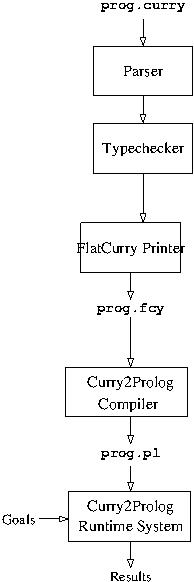
\includegraphics[scale=0.85]{pakcs_overview.jpg}
\end{center}\vspace{-5ex}
\caption{Overview of \CYS\label{fig-pakcs}}
\end{figure}

\section{Overview of the \CYS Distribution}

A schematic overview of the various components contained in
the distribution of \CYS and the
translation process of programs inside \CYS is shown in
Figure~\ref{fig-pakcs} on page~\pageref{fig-pakcs}.
In this figure, boxes denote different components of \CYS
and names in boldface denote files containing
various intermediate representations during the translation
process (see Section~\ref{sec-auxfiles} below).
The \CYS distribution contains a front end for reading (parsing and
type checking) Curry programs that can be also used by
other Curry implementations.
The back end (formerly known as ``Curry2Prolog''\index{Curry2Prolog})
compiles Curry programs into Prolog programs.
It also support constraint solvers for
arithmetic constraints over real numbers and finite domain constraints,
and further libraries for GUI programming, meta-programming etc.
Currently, it does not implement encapsulated search in full generality
(only a strict version of \code{findall} is supported),
and concurrent threads are not executed in a fair manner.


%%% Local Variables: 
%%% mode: latex
%%% TeX-master: "manual"
%%% End: 

\section{Auxiliary Files}
\label{sec-auxfiles}

During the translation and execution of a Curry program with \CYS,
various intermediate representations of the source program are created
and stored in different files which are shortly explained in this section.
If you use \CYS, it is not necessary to know about
these auxiliary files because they are automatically generated
and updated. You should only remember the command for deleting
all auxiliary files (\ccode{cleancurry}, see Section~\ref{sec-general})
to clean up your directories.

The various components of \CYS create
the following auxiliary files.
\begin{description}
\item[\code{prog.fcy}:] This file contains the Curry program
in the so-called ``FlatCurry'' representation where all functions are global
(i.e., lambda lifting has been performed) and pattern matching
is translated into explicit case/or expressions
(compare Appendix~\ref{sec-flatcurry}).
This representation might be useful for other back ends and
compilers for Curry and is the basis doing meta-programming in Curry.
This file is implicitly
generated when a program is read by \CYS.
It can be also explicitly generated by the Curry front end\pindex{cymake}
\begin{curry}
cymake --flat -i$\cyshome$/lib -i$\cyshome$/lib/meta prog
\end{curry}
The FlatCurry representation of a Curry program is usually
generated by the front-end after parsing, type checking and eliminating
local declarations.
If $dir$ is the directory where the Curry program is stored,
the corresponding FlatCurry program is stored in the directory
\ccode{$dir$/.curry}.

\item[\code{prog.fint}:] This file contains the interface
of the program in the so-called ``FlatCurry'' representation,
i.e., it is similar to \code{prog.fcy} but contains only exported
entities and the bodies of all functions omitted (i.e., ``external'').
This representation is useful for providing a fast access
to module interfaces.
It can be also implicitly generated by the Curry front end\pindex{cymake}
\begin{curry}
cymake --flat -i$\cyshome$/lib -i$\cyshome$/lib/meta prog
\end{curry}
and stored in the same directory as \code{prog.fcy}.

\item[\code{prog.pl}:] This file contains a Prolog program
as the result of translating the Curry program with \CYS.
If $dir$ is the directory where the Curry program is stored,
the corresponding Prolog program is stored in the directory
\ccode{$dir$/.curry/pakcs}.

\item[\code{prog.po}:] This file contains the Prolog program
\code{prog.pl} in an intermediate format for faster loading.
This file is stored in the same directory as \code{prog.pl}.

\item[\code{prog}:] This file contains the executable
after compiling and saving a program with \CYS
(see Section~\ref{sec:pakcs-commands}).

\end{description}


%%% Local Variables: 
%%% mode: latex
%%% TeX-master: "manual"
%%% End: 

\section{External Functions}
\label{sec-external-functions}

\index{function!external}\index{external function}
Currently, \CYS has no general interface to external functions.
Therefore, if a new external function should be added
to the system, this function must be declared as \code{external}
in the Curry source code
and then an implementation for this external function
must be inserted in the corresponding back end.
An external function is defined as follows in the Curry source code:
\begin{enumerate}
\item
Add a type declaration for the external function somewhere
in the body of the appropriate file (usually, the prelude
or some system module).
\item
For external functions it is not allowed to define any
rule since their semantics is determined by an external implementation.
Instead of the defining rules, you have to write
\begin{curry}
f external
\end{curry}
somewhere in the file containing the type declaration for 
the external function \code{f}.
\end{enumerate}
For instance, the addition on integers can be declared as
an external function as follows:
\begin{curry}
(+) :: Int -> Int -> Int
(+) external
\end{curry}
The further modifications to be done for an inclusion of
an external function has to be done in the back end.
A new external function is added to the back end of \CYS
by informing the compiler about the existence of an external function
and adding an implementation of this function in the run-time
system. Therefore, the following items must be added
in the \CYS compiler system:
\begin{enumerate}
\item
If the Curry module \code{Mod} contains external functions,
there must be a file named \code{Mod.prim_c2p} containing the
specification of these external functions. The contents of this file
is in XML format and has the following general structure:\footnote{%
\url{http://www.informatik.uni-kiel.de/~pakcs/primitives.dtd} contains a DTD
describing the exact structure of these files.}
\begin{curry}
<primitives>
  $\textit{specification of external function~}f_1$
  $\ldots$
  $\textit{specification of external function~}f_n$
</primitives>
\end{curry}
The specification of an external function $f$
with arity $n$ has the form
\begin{curry}
<primitive name="$f$" arity="$n$">
  <library>lib</library>
  <entry>pred</entry>
</primitive>
\end{curry}
where \code{lib} is the Prolog library (stored in the directory of the
Curry module or in the global directory
\code{\cyshome/curry2prolog/lib_src}) containing the code implementing this
function and \code{pred} is a predicate name in this library
implementing this function. Note that the function $f$ must be
declared in module \code{Mod}: either as an external function
or defined in Curry by equations. In the latter case,
the Curry definition is not translated but calls to this function
are redirected to the Prolog code specified above.

Furthermore, the list of specifications can also contain entries of the form
\begin{curry}
<ignore name="$f$" arity="$n$" />
\end{curry}
for functions $f$ with arity $n$ that are declared in module \code{Mod}
but should be ignored for code generation, e.g., since they are
never called w.r.t.\ to the current implementation of external functions.
For instance, this is useful when functions that can
be defined in Curry should be (usually more efficiently) are implemented
as external functions.

Note that the arguments are passed in their current (possibly unevaluated) form.
Thus, if the external function requires the arguments to be evaluated
in a particular form, this must be done before calling the external function.
For instance, the external function for adding two integers
requires that both arguments must be evaluated to non-variable head normal form
(which is identical to the ground constructor normal form). Therefore,
the function \ccode{+} is specified in the prelude by
\begin{curry}
(+)   :: Int -> Int -> Int
x + y = (prim_Int_plus $\$$# y) $\$$# x

prim_Int_plus :: Int -> Int -> Int
prim_Int_plus external
\end{curry}
where \code{prim_Int_plus} is the actual external function implementing
the addition on integers. Consequently, the specification file
\code{Prelude.prim_c2p} has an entry of the form
\begin{curry}
<primitive name="prim_Int_plus" arity="2">
  <library>prim_standard</library>
  <entry>prim_Int_plus</entry>
</primitive>
\end{curry}
where the Prolog library \code{prim_standard.pl} contains the Prolog code
implementing this function.

\item
For most external functions, a \emph{standard interface} is
generated by the compiler so that an $n$-ary function can be
implemented by an $(n+1)$-ary predicate where the last argument must
be instantiated to the result of evaluating the function.  The
standard interface can be used if all arguments are ensured to be
fully evaluated (e.g., see definition of \code{(+)} above) and no
suspension control is necessary, i.e., it is ensured that the
external function call does not suspend for all arguments.
Otherwise, the raw interface (see below) must be used.  For
instance, the Prolog code implementing \code{prim_Int_plus}
contained in the Prolog library \code{prim_standard.pl} is as
follows (note that the arguments of \code{(+)} are passed in reverse
order to \code{prim_Int_plus} in order to ensure a left-to-right
evaluation of the original arguments by the calls to \code{(\$\#)}):
\begin{curry}
prim_Int_plus(Y,X,R) :- R is X+Y.
\end{curry}

\item
The \emph{standard interface for I/O actions}, i.e., external functions
with result type \code{IO~a}, assumes that the I/O action
is implemented as a predicate (with a possible side effect)
that instantiates the last argument to the returned value of type \ccode{a}.
For instance, the primitive predicate \code{prim_getChar}
implementing prelude I/O action \code{getChar}
can be implemented by the Prolog code
\begin{curry}
prim_getChar(C) :- get_code(N), char_int(C,N).
\end{curry}
where \code{char_int} is a predicate relating the internal
Curry representation of a character with its ASCII value.

\item
If some arguments passed to the external functions are not fully evaluated
or the external function might suspend, the implementation must follow
the structure of the \CYS run-time system by using
the \emph{raw interface}. In this case, the name of the external entry
must be suffixed by \ccode{[raw]} in the \code{prim_c2p} file.
For instance, if we want to use the raw interface for the external function
\code{prim_Int_plus},
the specification file \code{Prelude.prim_c2p} must have an entry of the form
\begin{curry}
<primitive name="prim_Int_plus" arity="2">
  <library>prim_standard</library>
  <entry>prim_Int_plus[raw]</entry>
</primitive>
\end{curry}
In the raw interface, the actual implementation of an $n$-ary external function consists
of the definition of an $(n+3)$-ary predicate $pred$.
The first $n$ arguments are the corresponding actual arguments.
The $(n+1)$-th argument is a free variable which must be
instantiated to the result of the function call after
successful execution. The last two arguments
control the suspension behavior of the function
(see \cite{AntoyHanus00FROCOS} for more details):
The code for the predicate $pred$
should only be executed when the $(n+2)$-th argument
is not free, i.e., this predicate has always the
SICStus-Prolog block declaration
\begin{curry}
?- block $pred$(?,$\ldots$,?,-,?).
\end{curry}
In addition, typical external functions should suspend
until the actual arguments are instantiated. This can be ensured
by a call to \code{ensureNotFree} or \code{(\$\#)}
before calling the external function. Finally, the
last argument (which is a free variable at call time)
must be unified with the $(n+2)$-th argument
after the function call is successfully evaluated
(and does not suspend). Additionally, the actual (evaluated) arguments
must be dereferenced before they are accessed.
Thus, an implementation
of the external function for adding integers is as follows in the raw interface:
\begin{curry}
?- block prim_Int_plus(?,?,?,-,?).
prim_Int_plus(RY,RX,Result,E0,E) :-
     deref(RX,X), deref(RY,Y), Result is X+Y, E0=E.
\end{curry}
Here, \code{deref} is a predefined predicate for dereferencing the
actual argument into a constant (and \code{derefAll} for dereferencing
complex structures).
\end{enumerate}
%
The Prolog code implementing the external functions must be accessible to the run-time
system of \CYS by putting it into the directory containing the corresponding
Curry module or into the system directory
\code{\cyshome/curry2prolog/lib_src}.
Then it will be automatically loaded into the run-time environment
of each compiled Curry program.

Note that arbitrary functions implemented in C or Java can be connected to
\CYS by using the corresponding interfaces of the underlying Prolog system.


%%% Local Variables: 
%%% mode: latex
%%% TeX-master: "manual"
%%% End: 


% Index
\addcontentsline{toc}{section}{Index}
\printindex

\end{document}
